\documentclass[11pt,a4paper,oneside]{book}
% =====================================================================
%  Preámbulo común — Econometría Financiera Aplicada
%  Estilo sobrio: texto en negro; color solo en código, salidas y gráficas
% =====================================================================
\usepackage[T1]{fontenc}
\usepackage[utf8]{inputenc}
\usepackage[spanish,es-noshorthands,es-tabla]{babel}
\usepackage{libertinus}           % Libertinus Serif (texto)
\usepackage[varqu,scaled=0.93]{zi4} % Inconsolata para código
\usepackage{microtype}
\usepackage[a4paper,top=3cm,bottom=3cm,inner=3cm,outer=2.6cm,headheight=14pt]{geometry}
\usepackage{setspace}\setstretch{1.1}
% ---------- Títulos sobrios en negro ----------
\usepackage{titlesec}
\titleformat{\chapter}[display]{\normalfont\bfseries\raggedright}{\large\scshape\mdseries\chaptertitlename\ \thechapter}{8pt}{\Huge}[\vspace{6pt}\titlerule]
\titlespacing*{\chapter}{0pt}{20pt}{36pt}
\titleformat{\section}{\normalfont\Large\bfseries}{\thesection}{0.8em}{}
\titleformat{\subsection}{\normalfont\large\bfseries}{\thesubsection}{0.8em}{}
\usepackage{amsmath,amsthm,mathtools}
\usepackage{libertinust1math}   % matemáticas Libertinus (incluye símbolos AMS)
\usepackage{bm}
\usepackage{booktabs,array,tabularx,multirow}
\usepackage{float}
\usepackage{enumitem}
\usepackage{xcolor}
\usepackage{graphicx}
\usepackage{needspace}
\usepackage{caption}
\captionsetup{font=small,labelfont=bf,labelsep=period}
\usepackage{pgfplots}\pgfplotsset{compat=1.16}
\usetikzlibrary{arrows.meta,fadings}
\usepackage{qrcode}
\tikzfading[name=nube, inner color=transparent!0, outer color=transparent!100]
\usepackage{fancyhdr}
\usepackage{hyperref}
% Enlaces en azul: índice, referencias a ecuaciones, teoremas, figuras, tablas, ejercicios y direcciones web
\definecolor{azulEnlace}{RGB}{0,70,170}
\hypersetup{colorlinks=true,linkcolor=azulEnlace,citecolor=azulEnlace,urlcolor=azulEnlace,filecolor=azulEnlace,
  linktoc=all}

% ---------- Encabezados (negro, discretos) ----------
\pagestyle{fancy}\fancyhf{}
\newcommand{\autorpie}{\footnotesize\scshape Jeel Cueva}          % nombre del autor en cada página
\newcommand{\obrapie}{\footnotesize\itshape Econometría Financiera Aplicada}
\fancyhead[L]{\small\nouppercase{\leftmark}}
\fancyhead[R]{\small\thepage}
\fancyfoot[L]{\autorpie}
\fancyfoot[R]{\obrapie}
\renewcommand{\headrulewidth}{0.3pt}
\renewcommand{\footrulewidth}{0pt}
\fancypagestyle{plain}{\fancyhf{}\fancyfoot[L]{\autorpie}\fancyfoot[C]{\small\thepage}\fancyfoot[R]{\obrapie}%
  \renewcommand{\headrulewidth}{0pt}}

% ---------- Entornos teóricos (amsthm clásico, sin color) ----------
\theoremstyle{plain}
\newtheorem{teorema}{Teorema}[chapter]
\newtheorem{proposicion}[teorema]{Proposición}
\newtheorem{lema}[teorema]{Lema}
\newtheorem{corolario}[teorema]{Corolario}
\theoremstyle{definition}
\newtheorem{definicion}[teorema]{Definición}
\newtheorem{ejemplo}[teorema]{Ejemplo}
\theoremstyle{remark}
\newtheorem{observacion}[teorema]{Observación}
\renewcommand{\qedsymbol}{$\blacksquare$}

% ---------- Ejercicios (sin fondos; solo filetes grises finos) ----------
\newcounter{ejres}[chapter]
\renewcommand{\theejres}{\thechapter.\arabic{ejres}}
\newenvironment{ejresuelto}[1]{\par\needspace{6\baselineskip}\bigskip
  \refstepcounter{ejres}\noindent{\color{gray!70}\rule{\linewidth}{0.4pt}}\par\smallskip
  \noindent\textbf{Ejercicio resuelto \theejres.}\ \textit{#1}\par\smallskip}%
  {\par\noindent{\color{gray!70}\rule{\linewidth}{0.4pt}}\par\bigskip}
\newcommand{\paso}[1]{\par\needspace{3\baselineskip}\smallskip\noindent\textbf{#1}\quad}
\newenvironment{conclusion}{\par\smallskip\noindent\textbf{Conclusión.}\ }{\par}
\newcommand{\enunciado}{\noindent\textsc{Enunciado.}\ }
\newcommand{\solucion}{\par\smallskip\noindent\textsc{Solución.}\ }

% Marcador de contenido que se completa con los datos descargados (se elimina en la versión final)
\newenvironment{pendiente}{\par\medskip\noindent\begin{tabular}{@{}|p{0.95\linewidth}@{}}\small\itshape
  [Pendiente de los datos]\ }{\end{tabular}\par\medskip}

% ---------- Código y salidas (único lugar con color, además de gráficas) ----------
\usepackage{listings}
\definecolor{cR}{RGB}{39,93,173}      % R
\definecolor{cPy}{RGB}{48,105,152}    % Python
\definecolor{cCom}{RGB}{96,125,96}
\definecolor{cStr}{RGB}{163,72,52}
\definecolor{cKey}{RGB}{122,40,120}
\lstset{basicstyle=\ttfamily\footnotesize,columns=fullflexible,keepspaces=true,
  breaklines=true,showstringspaces=false,tabsize=2,
  commentstyle=\color{cCom},stringstyle=\color{cStr},keywordstyle=\color{cKey}\bfseries,
  literate={á}{{\'a}}1 {é}{{\'e}}1 {í}{{\'i}}1 {ó}{{\'o}}1 {ú}{{\'u}}1 {ñ}{{\~n}}1
           {Á}{{\'A}}1 {É}{{\'E}}1 {Í}{{\'I}}1 {Ó}{{\'O}}1 {Ú}{{\'U}}1 {Ñ}{{\~N}}1 {¿}{{?`}}1 {¡}{{!`}}1
           {ü}{{\"u}}1 {²}{{\textsuperscript{2}}}1 {³}{{\textsuperscript{3}}}1 {°}{{\textdegree}}1 {×}{{$\times$}}1 {≈}{{$\approx$}}1 {→}{{$\to$}}1 {–}{{--}}1 {—}{{---}}1 {±}{{$\pm$}}1}
\lstdefinestyle{codR}{language=R,frame=leftline,framerule=1.2pt,rulecolor=\color{cR},xleftmargin=8pt,
  framexleftmargin=6pt,title={\small\sffamily\color{cR}R}}
\lstdefinestyle{codPy}{language=Python,frame=leftline,framerule=1.2pt,rulecolor=\color{cPy},
  xleftmargin=8pt,framexleftmargin=6pt,title={\small\sffamily\color{cPy}Python}}
\lstdefinestyle{salida}{language={},backgroundcolor=\color{gray!8},frame=none,xleftmargin=8pt,
  framexleftmargin=6pt,title={\small\sffamily\color{gray}Salida}}
\lstnewenvironment{codigoR}{\lstset{style=codR}}{}
\lstnewenvironment{codigoPy}{\lstset{style=codPy}}{}
\lstnewenvironment{salida}{\lstset{style=salida}}{}

% ---------- Gráficas: paleta sobria y consistente ----------
\definecolor{g1}{RGB}{31,60,110}    % azul oscuro
\definecolor{g2}{RGB}{166,62,46}    % rojo ladrillo
\definecolor{g3}{RGB}{104,120,56}   % verde oliva
\definecolor{g4}{RGB}{120,120,120}  % gris
\pgfplotsset{libro/.style={axis lines=left,every axis plot/.append style={thick},
  tick label style={font=\footnotesize},label style={font=\small},
  legend style={font=\footnotesize,draw=none,fill=none},legend cell align=left,
  /pgf/number format/.cd,use comma,1000 sep={\,}}}

% ---------- Notación ----------
\newcommand{\E}{\mathbb{E}}
\newcommand{\Var}{\operatorname{Var}}
\newcommand{\Cov}{\operatorname{Cov}}
\newcommand{\soles}{S/\,}

% ---------- Código y salidas leídos de los archivos ejecutados ----------
\newcommand{\archivoR}[1]{\lstinputlisting[style=codR]{codigo/R/#1}}
\newcommand{\archivoPy}[1]{\lstinputlisting[style=codPy]{codigo/Python/#1}}
\newcommand{\salidaR}[1]{\lstinputlisting[style=salida,title={\small\sffamily\color{gray}Salida en R}]{salidas/#1}}
\newcommand{\salidaPy}[1]{\lstinputlisting[style=salida,title={\small\sffamily\color{gray}Salida en Python}]{salidas/#1}}
\newcommand{\RvsPy}{\par\smallskip\noindent\textbf{Nota sobre el código.}\ }
% Sitio web del libro: programas en R y Python, salidas y datos de cada ejercicio
\newcommand{\sitioweb}{https://github.com/JeelCueva/Econometr-a-Financiera-Aplicada-2026}
\newcommand{\codigoweb}[1]{\par\smallskip\noindent{\small\sffamily Programas de este ejercicio en el repositorio
  del libro: \href{\sitioweb/blob/HEAD/codigo/R/#1.R}{\texttt{\detokenize{#1}.R}} (R) y
  \href{\sitioweb/blob/HEAD/codigo/Python/#1.py}{\texttt{\detokenize{#1}.py}} (Python); datos en la carpeta
  \href{\sitioweb/tree/HEAD/datos}{\texttt{datos}}.}\par\smallskip}
% Tabla "Cómo leer la salida" de cada ejercicio (archivos en lecturas/)
\usepackage{xltabular}
\newcommand{\lectura}[1]{\IfFileExists{lecturas/#1.tex}{\input{lecturas/#1}}{}}
\setlength{\emergencystretch}{1.5em}


\title{\textbf{Econometría Financiera Aplicada}\\[6pt]
\large Teoría, demostraciones y práctica con datos reales del Perú y del mundo}
\author{Jeel Cueva}
\hypersetup{pdftitle={Econometría Financiera Aplicada},pdfauthor={Jeel Cueva}}
\date{Noviembre de 2026}

\begin{document}
\frontmatter
% =====================================================================
%  Portada, anteportada y créditos — Econometría Financiera Aplicada (Jeel Cueva)
%  Banda superior: manchas difuminadas en cobre, vino y turquesa; bloque inferior azul petróleo.
%  La pequeña curva cobre del pie es el índice S&P/BVL Perú General semanal 2015-2026 (BCRP).
% =====================================================================
% Paleta andina: azul petróleo profundo, cobre (minería peruana), turquesa, vino y arena
\definecolor{petroleo}{RGB}{14,72,86}
\definecolor{petroleoOscuro}{RGB}{8,46,58}
\definecolor{tintaPortada}{RGB}{22,18,30}
\definecolor{cobre}{RGB}{222,140,82}
\definecolor{cobreClaro}{RGB}{242,186,140}
\definecolor{turquesaClaro}{RGB}{128,214,214}
\begin{titlepage}
\newgeometry{margin=0pt}
\thispagestyle{empty}
\begin{tikzpicture}[remember picture,overlay]
  % ---- banda superior: fondo tinta y manchas de color difuminadas ----
  \coordinate (A) at ([yshift=-9.4cm]current page.north west);
  \begin{scope}
    \clip (current page.north west) rectangle (A -| current page.east);
    \fill[tintaPortada] (current page.north west) rectangle (A -| current page.east);
    \definecolor{m1}{RGB}{122,30,62}\definecolor{m2}{RGB}{214,120,60}\definecolor{m3}{RGB}{40,170,170}
    \definecolor{m4}{RGB}{232,190,120}\definecolor{m5}{RGB}{176,52,48}\definecolor{m6}{RGB}{20,110,120}
    \foreach \x/\y/\r/\c in {2.5/-3.5/8/m1, 10.5/-1.0/7.5/m2, 13.5/-8.5/7/m3, 19.5/-2.0/6.5/m4,
                             21.5/-9.0/6/m5, 5.5/-10.0/5.5/m6, 16.0/-4.5/4.5/m3}{
      \fill[\c,fill opacity=0.85,path fading=nube] ([xshift=\x cm,yshift=\y cm]current page.north west) circle (\r cm);}
  \end{scope}
  % ---- bloque inferior ocre ----
  \shade[top color=petroleo,bottom color=petroleoOscuro] (A) rectangle (current page.south east);
  % ---- filetes blancos: vertical a la izquierda y horizontal entre bloques ----
  \draw[cobre,line width=0.9pt] ([xshift=1.9cm]current page.north west) -- ([xshift=1.9cm]current page.south west);
  \draw[cobre,line width=1.2pt] (A) -- (A -| current page.east);
  \draw[cobre,line width=0.6pt] ([yshift=-4.6cm]A) -- ++(1.9cm,0);
  % ---- textos de la banda ----
  \node[anchor=north west,inner sep=0pt,font=\sffamily\large,text=cobreClaro]
       at ([xshift=2.6cm,yshift=-1.3cm]current page.north west) {Teoría, demostraciones y datos reales};
  \node[anchor=south west,inner sep=0pt,font=\sffamily\fontsize{28}{32}\selectfont,text=white]
       at ([xshift=2.6cm,yshift=0.7cm]A) {Jeel Cueva};
  % ---- título ----
  \node[anchor=north west,inner sep=0pt,align=left,text=white,font=\sffamily\fontsize{50}{56}\selectfont]
       at ([xshift=2.6cm,yshift=-1.1cm]A) {Econometría\\Financiera\\Aplicada};
  \node[anchor=north west,inner sep=0pt,align=left,text=cobreClaro,font=\sffamily\fontsize{22}{27}\selectfont]
       at ([xshift=2.6cm,yshift=-7.6cm]A) {con ejemplos en R y Python};
  \node[anchor=north west,inner sep=0pt,align=left,text=turquesaClaro,font=\sffamily\itshape\fontsize{20}{24}\selectfont]
       at ([xshift=2.6cm,yshift=-9.4cm]A) {Primera edición};
  % ---- marca del pie: la curva del índice de la BVL ----
  \begin{scope}[shift={([xshift=-7.3cm,yshift=2.2cm]current page.south east)}]
    \begin{axis}[width=4.6cm,height=2.4cm,scale only axis,axis lines=none,xmin=0,xmax=620,ymin=40,ymax=440,ymode=log]
      \addplot[cobre,line width=1.3pt] table[x=t,y=v] {graficos/portada_bvl.dat};
    \end{axis}
  \end{scope}
  \node[anchor=north east,inner sep=0pt,font=\sffamily\small,text=cobreClaro]
       at ([xshift=-2.7cm,yshift=1.95cm]current page.south east) {Bolsa de Valores de Lima, 2015--2026};
\end{tikzpicture}
\restoregeometry
\end{titlepage}

% ---------------- Anteportada ----------------
\thispagestyle{plain}
\vspace*{1.2cm}
\begin{flushleft}
{\large Jeel Cueva}\\[1.6cm]
{\fontsize{30}{36}\selectfont Econometría Financiera Aplicada}\\[10pt]
{\Large con ejemplos en R y Python}\\[14pt]
{\normalsize Teoría, demostraciones y práctica con datos reales del Perú y del mundo}\\[18pt]
{\small Primera edición}
\end{flushleft}
\vspace*{\fill}
\begin{flushleft}\small
Lima, 2026
\end{flushleft}
\clearpage

% ---------------- Página de créditos ----------------
\thispagestyle{plain}
\vspace*{\fill}
\begin{flushleft}\small
\textbf{Econometría Financiera Aplicada}\\
con ejemplos en R y Python\\[10pt]
\copyright\ 2026 Jeel Cueva. Todos los derechos reservados.\\
Obra escrita y editada por su autor.\\[10pt]
Primera edición, noviembre de 2026. Lima, Perú.\\[10pt]
Programas en R y Python, salidas completas y bases de datos (repositorio en GitHub):\\
\url{\sitioweb}\\[10pt]
Los datos provienen de fuentes públicas: Banco Central de Reserva del Perú (BCRPData), Yahoo Finance,
Kenneth R. French Data Library, base de datos de Robert Shiller, EIA de EE.\,UU., CBOE y otras que se
citan en cada capítulo. Todos los resultados numéricos del libro son la salida real de los programas
publicados en ese repositorio.\\[10pt]
Compuesto en \LaTeX{} con la familia tipográfica Libertinus.
\end{flushleft}
\clearpage

% =====================================================================
%  Prefacio — Econometría Financiera Aplicada (Jeel Cueva)
% =====================================================================
\chapter*{Prefacio}
\addcontentsline{toc}{chapter}{Prefacio}
\markboth{Prefacio}{Prefacio}

Este libro nació de una necesidad concreta: un texto de econometría financiera en español que llevara al
lector desde las nociones básicas de precios y rendimientos hasta los modelos que hoy se usan en la gestión
de riesgos, la valoración de activos y el pronóstico, sin renunciar al rigor de las demostraciones ni al
trabajo con datos reales. Cada resultado teórico se demuestra paso a paso y cada técnica se aplica a series
reales del Perú y del mundo: el índice de la Bolsa de Valores de Lima y el tipo de cambio del Banco Central
de Reserva del Perú, acciones peruanas que cotizan en Nueva York, el petróleo, el S\&P 500, las carteras de
Fama y French y la curva de rendimientos de los Estados Unidos, entre otras.

El libro tiene veintiún capítulos y tres apéndices. Los primeros capítulos tratan los rendimientos, sus
hechos estilizados y la regresión en finanzas; les siguen los modelos de series de tiempo, la volatilidad
condicional, los modelos multivariados, el valor en riesgo, los modelos de factores, las tasas de interés,
los estudios de eventos, los cambios de régimen, las cópulas, los datos de panel y el aprendizaje
automático. El último capítulo integra todo en un proyecto completo. Cada capítulo incluye ejercicios
resueltos y ejercicios propuestos.

Todos los ejercicios resueltos siguen la misma estructura: el enunciado, el planteamiento y los pasos de
la solución, la salida real del programa en R, una tabla \emph{Cómo leer la salida} que interpreta cada
indicador que aparece en ella y una conclusión. La tabla está pensada para que el lector no solo obtenga
un número, sino que sepa qué significa, cuándo es grande o pequeño y qué decisión permite tomar.

Para que el libro no se hiciera excesivamente extenso, los programas no se imprimen. El código completo en
R y en Python de cada ejercicio, la salida que produce en ambos lenguajes y todas las bases de datos están
en el repositorio del libro en GitHub:
\begin{center}
\begin{tabular}{@{}c@{\qquad}l@{}}
\raisebox{-0.5\height}{\qrcode[height=2.6cm]{\sitioweb}} &
\begin{minipage}{0.62\linewidth}\raggedright
\href{\sitioweb}{\nolinkurl{\sitioweb}}\\[6pt]
\small Escanee el código con el teléfono o haga clic en la dirección. Antes de la salida de cada ejercicio
hay enlaces directos a sus programas en el repositorio.
\end{minipage}
\end{tabular}
\end{center}
El repositorio está organizado como el proyecto del libro. La carpeta \texttt{codigo} contiene un programa
por ejercicio en R (\texttt{codigo/R}) y en Python (\texttt{codigo/Python}); por ejemplo, los del
Ejercicio~1.1 son \texttt{cap01\_ej01.R} y \texttt{cap01\_ej01.py}. La carpeta \texttt{salidas} contiene la
salida de cada programa en ambos lenguajes, y la carpeta \texttt{datos} reúne los archivos CSV con un
archivo \texttt{FUENTES.txt} que documenta sus fuentes y fechas de descarga. Todo el material puede
descargarse en un solo archivo con el botón \emph{Code} $\rightarrow$ \emph{Download ZIP} de GitHub.
Las cifras del libro son exactamente las que producen esos programas, de
modo que el lector puede reproducir cualquier resultado y modificar los programas para aplicarlos a sus
propios datos.

Los datos son reales y públicos. Las series peruanas provienen de BCRPData y de Yahoo Finance; las
internacionales, de bases académicas y oficiales que se citan en cada capítulo. Al trabajar con ellas
aparecieron errores en las propias fuentes, como un dato erróneo del índice bursátil o un dividendo
registrado dos veces, que el libro no oculta: se detectan, se explican y se corrigen, porque reconocerlos
es parte del oficio del econometrista.

El libro está pensado tanto para cursos universitarios de pregrado avanzado y maestría como para el
estudio personal. Se supone que el lector conoce la estadística y el álgebra lineal de un primer curso;
los resultados que se usan sin demostrar en el texto principal se reúnen en los Apéndices~A y~B.

Agradeceré a los lectores que me hagan llegar sus comentarios y los errores que encuentren, para
corregirlos en futuras ediciones.

\bigskip
\noindent Lima, noviembre de 2026\hfill Jeel Cueva

\tableofcontents

\mainmatter
\part{Fundamentos}
% =====================================================================
%  Capítulo 1. Datos financieros: precios y rendimientos
% =====================================================================
\chapter{Datos financieros: precios y rendimientos}\label{cap:rendimientos}

\section*{Objetivos de aprendizaje}
Al terminar este capítulo, el lector podrá:
\begin{enumerate}[label=\arabic*.,leftmargin=*]
  \item Distinguir el precio de cierre del precio ajustado y explicar cómo los dividendos y los
        desdoblamientos (\emph{splits}) modifican una serie de precios.
  \item Definir los rendimientos simples y logarítmicos, demostrar sus propiedades de agregación y
        elegir el tipo adecuado según el problema (agregación en el tiempo o entre activos).
  \item Calcular el rendimiento en soles de una inversión en dólares y descomponerlo en la parte del
        activo y la parte del tipo de cambio.
  \item Convertir rendimientos nominales en reales y medir excesos de rendimiento.
  \item Anualizar medias y volatilidades, y entender cuándo la regla de la raíz del tiempo es válida.
  \item Preparar series financieras reales para el análisis: calendarios de negociación distintos,
        datos faltantes y sincronización de mercados.
\end{enumerate}

\section*{Motivación}
Un inversionista en Lima puede comprar acciones de Credicorp en la Bolsa de Valores de Lima (BVL) o
en la Bolsa de Nueva York; puede invertir en Southern Copper, cuyo precio depende del cobre, o en un
fondo que replica el mercado peruano. En todos los casos, la primera pregunta es la misma: \emph{¿cuánto
ganó?} La respuesta parece trivial, pero no lo es. Depende de si se cuentan los dividendos, de si se mide
en dólares o en soles, de si se descuenta la inflación, de la frecuencia de los datos y de cómo se
promedian las ganancias de varios períodos. Dos analistas que usan los mismos precios pueden reportar
rendimientos distintos y ambos tener razón, si cada uno explica qué midió.

Este capítulo fija el lenguaje que usaremos en todo el libro. Todo modelo econométrico posterior
(regresión, ARMA, GARCH, VAR, valor en riesgo) se estima sobre rendimientos, no sobre precios, así que
cualquier error en este punto se arrastra a todos los resultados.

% ---------------------------------------------------------------------
\section{Precios: de cierre, ajustados y en distintas monedas}
% ---------------------------------------------------------------------

Sea $P_t$ el precio de cierre de un activo en el día $t$, es decir, el último precio negociado en la
sesión. Los proveedores de datos, como Yahoo Finance, publican además un \emph{precio de cierre
ajustado}, $P^{a}_t$, que corrige la serie histórica por dividendos y desdoblamientos para que los
cambios de precio reflejen solo ganancias o pérdidas del inversionista.

\begin{definicion}[Fecha ex-dividendo]
Cuando una empresa reparte un dividendo $D_t$ por acción, la \emph{fecha ex-dividendo} $t$ es el primer
día en que quien compra la acción ya no recibe ese dividendo. En esa fecha el precio tiende a caer
aproximadamente en $D_t$, sin que el accionista haya perdido riqueza: la diferencia la recibe en efectivo.
\end{definicion}

Si se calculara el rendimiento con precios de cierre, la caída del día ex-dividendo aparecería como una
pérdida que no existió. Por eso se define el rendimiento total del período.

\begin{definicion}[Rendimiento total]
El rendimiento total simple entre $t-1$ y $t$ de un activo que reparte $D_t$ en $t$ es
\begin{equation}\label{eq:rtotal}
  R^{\mathrm{tot}}_t=\frac{P_t+D_t-P_{t-1}}{P_{t-1}}=\frac{P_t+D_t}{P_{t-1}}-1 .
\end{equation}
\end{definicion}

\subsection{El ajuste multiplicativo de los precios}

Los proveedores de datos no publican $D_t$ junto a cada precio; incorporan el dividendo directamente
en la serie de precios mediante un factor multiplicativo. La regla habitual es la siguiente: cuando hay
un dividendo con fecha ex-dividendo $t$, todos los precios \emph{anteriores} a $t$ se multiplican por
\begin{equation}\label{eq:factor}
  f_t=1-\frac{D_t}{P_{t-1}}=1-d_t,\qquad d_t\equiv\frac{D_t}{P_{t-1}},
\end{equation}
donde $d_t$ es el rendimiento por dividendo del día. Los factores de distintos dividendos se acumulan
multiplicándose; los precios posteriores al último evento no se modifican. En el
Ejercicio~\ref{ej:dividendos} comprobaremos con datos reales que la serie ajustada de Yahoo Finance
sigue esta regla.

\begin{proposicion}[Rendimiento con precios ajustados]\label{prop:ajuste}
Con el ajuste \eqref{eq:factor}, el rendimiento simple calculado con precios ajustados en la fecha
ex-dividendo es
\[
  1+R^{a}_t=\frac{P^{a}_t}{P^{a}_{t-1}}=\frac{P_t}{P_{t-1}-D_t},
\]
y su diferencia con el rendimiento total \eqref{eq:rtotal} es
\begin{equation}\label{eq:difajuste}
  R^{a}_t-R^{\mathrm{tot}}_t=\frac{d_t}{1-d_t}\,R^{\mathrm{tot}}_t .
\end{equation}
En los días sin dividendo, $R^{a}_t$ coincide exactamente con el rendimiento calculado con precios de
cierre.
\end{proposicion}

\begin{proof}
Sea $C$ el producto de los factores de todos los eventos posteriores a $t$ (si no hay ninguno, $C=1$).
El precio de $t$ solo recibe esos factores; el de $t-1$, que es anterior a la fecha ex-dividendo, recibe
además el factor $f_t$:
\begin{align*}
  P^{a}_t     &= C\,P_t,\\
  P^{a}_{t-1} &= C\,f_t\,P_{t-1}\\
              &= C\Bigl(1-\frac{D_t}{P_{t-1}}\Bigr)P_{t-1}\\
              &= C\,(P_{t-1}-D_t).
\end{align*}
Dividiendo ambas expresiones:
\begin{align*}
  1+R^{a}_t &= \frac{P^{a}_t}{P^{a}_{t-1}}\\
            &= \frac{C\,P_t}{C\,(P_{t-1}-D_t)}\\
            &= \frac{P_t}{P_{t-1}-D_t}.
\end{align*}
Para la diferencia con el rendimiento total, restamos los rendimientos brutos con denominador común:
\begin{align*}
  R^{a}_t-R^{\mathrm{tot}}_t
    &= \frac{P_t}{P_{t-1}-D_t}-\frac{P_t+D_t}{P_{t-1}}\\
    &= \frac{P_tP_{t-1}-(P_t+D_t)(P_{t-1}-D_t)}{P_{t-1}(P_{t-1}-D_t)}\\
    &= \frac{P_tP_{t-1}-P_tP_{t-1}+P_tD_t-D_tP_{t-1}+D_t^2}{P_{t-1}(P_{t-1}-D_t)}\\
    &= \frac{D_t\,(P_t+D_t-P_{t-1})}{P_{t-1}(P_{t-1}-D_t)}\\
    &= \frac{D_t}{P_{t-1}}\cdot\frac{P_t+D_t-P_{t-1}}{P_{t-1}}\cdot\frac{P_{t-1}}{P_{t-1}-D_t}\\
    &= d_t\cdot R^{\mathrm{tot}}_t\cdot\frac{1}{1-d_t}.
\end{align*}
Finalmente, si en $t$ no hay dividendo, $P_t$ y $P_{t-1}$ reciben exactamente los mismos factores (los de
eventos posteriores a $t$), que se cancelan en el cociente.
\end{proof}

\begin{observacion}
La diferencia \eqref{eq:difajuste} es el producto de dos cantidades pequeñas: el rendimiento por
dividendo del día ($d_t$, típicamente menor que 0,03) y el rendimiento diario ($R^{\mathrm{tot}}_t$,
típicamente de pocos puntos porcentuales). Es, por tanto, un efecto de \emph{segundo orden}: en la
práctica, el rendimiento con precios ajustados equivale al rendimiento total. La interpretación
económica es que $R^a_t$ supone que el dividendo se reinvierte en la propia acción al precio de cierre
del día anterior a la fecha ex-dividendo, mientras que $R^{\mathrm{tot}}_t$ lo trata como efectivo.
\end{observacion}

\begin{proposicion}[Desdoblamientos]\label{prop:split}
Si en $t$ hay un desdoblamiento $k\!:\!1$ (cada acción se convierte en $k$ acciones) y los precios
anteriores a $t$ se multiplican por $1/k$, el rendimiento con precios ajustados en $t$ coincide con el
rendimiento económico del accionista.
\end{proposicion}
La demostración se deja como ejercicio propuesto (Ejercicio~\ref{prop:ejsplit}).

\subsection{Precios en otra moneda}

Muchas acciones peruanas o vinculadas al Perú (Credicorp, Southern Copper, Buenaventura) se negocian en
dólares en Nueva York. Para un inversionista que mide su riqueza en soles, el valor en soles de una
acción es
\[
  V_t=P_t\,S_t,
\]
donde $P_t$ es el precio en dólares y $S_t$ es el tipo de cambio en soles por dólar. Como fuente
oficial del tipo de cambio usaremos el \emph{tipo de cambio interbancario} que publica el Banco Central
de Reserva del Perú (BCRP) en BCRPData; en la Sección~\ref{sec:datos} veremos los cuidados para combinar
ambas series.

% ---------------------------------------------------------------------
\section{Rendimientos simples}
% ---------------------------------------------------------------------

\begin{definicion}[Rendimiento simple]
El \emph{rendimiento simple neto} de un período es $R_t=\dfrac{P_t-P_{t-1}}{P_{t-1}}=\dfrac{P_t}{P_{t-1}}-1$
y el \emph{rendimiento simple bruto} es $1+R_t=P_t/P_{t-1}$. Si el activo paga dividendos, se usa
$P_t^{a}$ o la fórmula \eqref{eq:rtotal}. Como $P_t\ge 0$, se cumple siempre $R_t\ge -1$: la pérdida
máxima es el total de lo invertido.
\end{definicion}

\begin{proposicion}[Agregación en el tiempo]\label{prop:multi}
El rendimiento simple bruto de $k$ períodos, $1+R_t(k)=P_t/P_{t-k}$, es el producto de los rendimientos
brutos de cada período:
\[
  1+R_t(k)=\prod_{j=0}^{k-1}\bigl(1+R_{t-j}\bigr).
\]
\end{proposicion}

\begin{proof}
Multiplicamos y dividimos por los precios intermedios $P_{t-1},\dots,P_{t-k+1}$:
\begin{align*}
  1+R_t(k) &= \frac{P_t}{P_{t-k}}\\
           &= \frac{P_t}{P_{t-1}}\cdot\frac{P_{t-1}}{P_{t-2}}\cdots\frac{P_{t-k+1}}{P_{t-k}}\\
           &= \prod_{j=0}^{k-1}\frac{P_{t-j}}{P_{t-j-1}}\\
           &= \prod_{j=0}^{k-1}\bigl(1+R_{t-j}\bigr).
\end{align*}
Cada precio intermedio aparece una vez en un numerador y una vez en un denominador, y se cancela
(producto telescópico).
\end{proof}

La consecuencia práctica es que los rendimientos simples \emph{no se suman} en el tiempo: una ganancia
de 10\,\% seguida de una pérdida de 10\,\% no deja al inversionista igual, sino con
$1{,}10\times 0{,}90-1=-1$\,\%.

\subsection{Rendimiento de un portafolio}

\begin{proposicion}[Agregación entre activos]\label{prop:portafolio}
Considere un portafolio de $N$ activos cuyo valor inicial es $W_{t-1}=\sum_i n_iP_{i,t-1}$, con $n_i$
unidades del activo $i$ y sin cambios de composición en el período. Si $w_i=n_iP_{i,t-1}/W_{t-1}$ es
la proporción del valor invertida en $i$, entonces
\[
  R_{p,t}=\sum_{i=1}^{N}w_i\,R_{i,t},\qquad \sum_{i=1}^N w_i=1 .
\]
\end{proposicion}

\begin{proof}
El valor final del portafolio es
\begin{align*}
  W_t &= \sum_{i=1}^N n_iP_{i,t}\\
      &= \sum_{i=1}^N n_iP_{i,t-1}\,(1+R_{i,t}).
\end{align*}
Dividiendo entre el valor inicial $W_{t-1}$:
\begin{align*}
  1+R_{p,t} &= \frac{W_t}{W_{t-1}}\\
            &= \sum_{i=1}^N\frac{n_iP_{i,t-1}}{W_{t-1}}\,(1+R_{i,t})\\
            &= \sum_{i=1}^N w_i\,(1+R_{i,t})\\
            &= \sum_{i=1}^N w_i+\sum_{i=1}^N w_iR_{i,t}\\
            &= 1+\sum_{i=1}^N w_iR_{i,t}.
\end{align*}
Restando 1 en ambos lados se obtiene el resultado.
\end{proof}

\begin{observacion}
Las ponderaciones $w_i$ son las del \emph{inicio} del período. Si el portafolio no se rebalancea, los
pesos cambian solos: el activo que más sube gana participación. Este hecho importa cuando se agregan
varios períodos (Ejercicio~\ref{ej:portafolio}).
\end{observacion}

% ---------------------------------------------------------------------
\section{Rendimientos logarítmicos}
% ---------------------------------------------------------------------

\begin{definicion}[Rendimiento logarítmico]
El \emph{rendimiento logarítmico} o \emph{rendimiento compuesto continuo} es
\[
  r_t=\ln(1+R_t)=\ln\frac{P_t}{P_{t-1}}=p_t-p_{t-1},\qquad p_t\equiv\ln P_t .
\]
\end{definicion}

El nombre ``compuesto continuo'' viene de lo siguiente: si una inversión crece a una tasa $r$ compuesta
$m$ veces por período, su valor bruto es $(1+r/m)^m$, que tiende a $e^{r}$ cuando $m\to\infty$. Entonces
$P_t=P_{t-1}e^{r_t}$, y $r_t$ es la tasa continua que lleva de $P_{t-1}$ a $P_t$.

\begin{proposicion}[Aditividad temporal]\label{prop:aditiva}
El rendimiento logarítmico de $k$ períodos es la suma de los rendimientos logarítmicos de un período:
\[
  r_t(k)\equiv\ln\frac{P_t}{P_{t-k}}=\sum_{j=0}^{k-1}r_{t-j}.
\]
\end{proposicion}

\begin{proof}
\begin{align*}
  r_t(k) &= \ln\frac{P_t}{P_{t-k}}\\
         &= \ln\prod_{j=0}^{k-1}(1+R_{t-j}) && \text{(Proposición~\ref{prop:multi})}\\
         &= \sum_{j=0}^{k-1}\ln(1+R_{t-j}) && \text{(logaritmo de un producto)}\\
         &= \sum_{j=0}^{k-1}r_{t-j}. && \qedhere
\end{align*}
\end{proof}

La aditividad es la razón principal por la que la econometría financiera trabaja con rendimientos
logarítmicos: si los rendimientos diarios son variables aleatorias, el rendimiento mensual es una
\emph{suma} de variables aleatorias, y para sumas existen resultados como la ley de los grandes números
y el teorema central del límite. Con rendimientos simples tendríamos productos, mucho más difíciles de
tratar.

\subsection{Relación entre ambos rendimientos}

\begin{proposicion}\label{prop:desigualdad}
Para todo $R_t>-1$ se cumple $r_t\le R_t$, con igualdad si y solo si $R_t=0$.
\end{proposicion}

\begin{proof}
Sea $g(x)=x-\ln(1+x)$ para $x>-1$. Su derivada es
\begin{align*}
  g'(x) &= 1-\frac{1}{1+x}\\
        &= \frac{x}{1+x},
\end{align*}
negativa en $(-1,0)$ y positiva en $(0,\infty)$. Por tanto, $g$ decrece hasta $x=0$ y crece después: su
mínimo global está en $x=0$, y es único. En ese punto
\begin{align*}
  g(0) &= 0-\ln 1\\
       &= 0.
\end{align*}
Así, $g(x)\ge0$ para todo $x>-1$, con igualdad solo en $x=0$. Con $x=R_t$:
\begin{align*}
  R_t-\ln(1+R_t) &\ge 0\\
  R_t-r_t        &\ge 0\\
  r_t            &\le R_t. && \qedhere
\end{align*}
\end{proof}

\begin{proposicion}[Aproximación de segundo orden]\label{prop:taylor}
Para todo $R_t>-1$ existe $\xi$ entre $0$ y $R_t$ tal que
\[
  r_t=R_t-\frac{R_t^2}{2(1+\xi)^2}.
\]
En particular, $r_t\approx R_t-\tfrac12R_t^2$ cuando $R_t$ es pequeño, y el error relativo de usar
$r_t$ en lugar de $R_t$ es del orden de $R_t/2$.
\end{proposicion}

\begin{proof}
Sea $h(x)=\ln(1+x)$. Sus derivadas son
\begin{align*}
  h(0)   &= 0,\\
  h'(x)  &= (1+x)^{-1}, \qquad h'(0)=1,\\
  h''(x) &= -(1+x)^{-2}.
\end{align*}
El teorema de Taylor con resto de Lagrange de orden dos alrededor de $0$ dice que existe $\xi$ entre $0$ y
$x$ tal que
\begin{align*}
  h(x) &= h(0)+h'(0)\,x+\tfrac12\,h''(\xi)\,x^2\\
       &= 0+1\cdot x-\tfrac12\,(1+\xi)^{-2}x^2\\
       &= x-\frac{x^2}{2(1+\xi)^2}.
\end{align*}
Con $x=R_t$ se obtiene el resultado. Si $R_t$ es pequeño, $\xi\approx0$ y $(1+\xi)^{-2}\approx1$, de
donde $r_t\approx R_t-\tfrac12R_t^2$.
\end{proof}

\begin{figure}[ht]
\centering
\begin{tikzpicture}
\begin{axis}[libro,width=10.5cm,height=7cm,xmin=-0.6,xmax=0.6,ymin=-0.95,ymax=0.65,
  xlabel={rendimiento simple $R$},ylabel={rendimiento},
  xtick={-0.6,-0.4,-0.2,0,0.2,0.4,0.6},ytick={-0.8,-0.6,-0.4,-0.2,0,0.2,0.4,0.6},
  legend pos=north west]
  \addplot[g4,dashed,domain=-0.6:0.6]{x}; \addlegendentry{$R$ (recta de $45^\circ$)}
  \addplot[g1,domain=-0.6:0.6,samples=120]{ln(1+x)}; \addlegendentry{$r=\ln(1+R)$}
  \addplot[g2,densely dotted,domain=-0.6:0.6,samples=60]{x-x^2/2}; \addlegendentry{$R-R^2/2$}
  \draw[g2,thin,{Stealth}-{Stealth}] (axis cs:-0.5,-0.5) -- (axis cs:-0.5,{ln(0.5)});
  \draw[g2,thin,{Stealth}-{Stealth}] (axis cs:0.5,0.5) -- (axis cs:0.5,{ln(1.5)});
  \node[font=\footnotesize,anchor=west] at (axis cs:-0.48,-0.6) {$0{,}193$};
  \node[font=\footnotesize,anchor=east] at (axis cs:0.48,0.45) {$0{,}095$};
\end{axis}
\end{tikzpicture}
\caption{Rendimiento logarítmico frente a rendimiento simple. La curva $\ln(1+R)$ está siempre por
debajo de la recta de $45^\circ$ (Proposición~\ref{prop:desigualdad}) y la parábola $R-R^2/2$ la
aproxima bien cerca de cero. La brecha es asimétrica: para $R=-0{,}5$ es $0{,}193$ y para $R=0{,}5$ es
$0{,}095$ (Ejercicio propuesto~\ref{prop:ejasimetria}).}
\label{fig:logsimple}
\end{figure}

\subsection{El costo de los rendimientos logarítmicos: los portafolios}

La aditividad en el tiempo tiene un precio: los rendimientos logarítmicos no se agregan linealmente
entre activos.

\begin{proposicion}\label{prop:logport}
Sea un portafolio con ponderaciones $w_i\ge 0$, $\sum_iw_i=1$. Su rendimiento logarítmico es
\[
  r_{p,t}=\ln\Bigl(\sum_{i=1}^Nw_i\,e^{r_{i,t}}\Bigr)\;\ge\;\sum_{i=1}^Nw_i\,r_{i,t},
\]
con igualdad si y solo si todos los $r_{i,t}$ con $w_i>0$ son iguales.
\end{proposicion}

\begin{proof}
Por la Proposición~\ref{prop:portafolio},
\begin{align*}
  1+R_{p,t} &= \sum_iw_i\,(1+R_{i,t})\\
            &= \sum_iw_i\,e^{r_{i,t}},\\
  r_{p,t}   &= \ln\Bigl(\sum_iw_i\,e^{r_{i,t}}\Bigr).
\end{align*}
La función $x\mapsto e^x$ es estrictamente convexa. Por la desigualdad de Jensen con pesos no negativos
que suman uno,
\begin{align*}
  \sum_iw_i\,e^{r_{i,t}} &\ge \exp\Bigl(\sum_iw_i\,r_{i,t}\Bigr)\\
  \ln\Bigl(\sum_iw_i\,e^{r_{i,t}}\Bigr) &\ge \sum_iw_i\,r_{i,t} && \text{(el logaritmo es creciente)}\\
  r_{p,t} &\ge \sum_iw_i\,r_{i,t},
\end{align*}
con igualdad solo si los $r_{i,t}$ de peso positivo coinciden.
\end{proof}

\begin{observacion}
En la práctica, para rendimientos diarios la diferencia $r_{p,t}-\sum_iw_ir_{i,t}$ es pequeña y muchos
trabajos empíricos usan la suma ponderada como aproximación. Para datos mensuales o anuales, o con
posiciones cortas ($w_i<0$, donde la desigualdad puede invertirse; Ejercicio~\ref{prop:ejcorto}), la
aproximación puede ser mala. La regla práctica de este libro es: \emph{rendimientos simples para
agregar activos; rendimientos logarítmicos para agregar en el tiempo y para modelar}.
\end{observacion}

% ---------------------------------------------------------------------
\section{Rendimientos en soles, reales y en exceso}
% ---------------------------------------------------------------------

\begin{proposicion}[Rendimiento en moneda local]\label{prop:moneda}
Sea $R^{\$}_t$ el rendimiento en dólares de un activo y $R^{S}_t=S_t/S_{t-1}-1$ la variación del tipo
de cambio (positiva cuando el sol se deprecia). El rendimiento en soles es
\[
  R^{\mathrm{S/}}_t=(1+R^{\$}_t)(1+R^{S}_t)-1=R^{\$}_t+R^{S}_t+R^{\$}_tR^{S}_t,
\]
y en logaritmos la descomposición es exacta y aditiva: $r^{\mathrm{S/}}_t=r^{\$}_t+\Delta\ln S_t$.
\end{proposicion}

\begin{proof}
Con $V_t=P_tS_t$:
\begin{align*}
  1+R^{\mathrm{S/}}_t &= \frac{V_t}{V_{t-1}}\\
                      &= \frac{P_tS_t}{P_{t-1}S_{t-1}}\\
                      &= \frac{P_t}{P_{t-1}}\cdot\frac{S_t}{S_{t-1}}\\
                      &= (1+R^{\$}_t)(1+R^{S}_t)\\
                      &= 1+R^{\$}_t+R^{S}_t+R^{\$}_tR^{S}_t.
\end{align*}
En logaritmos:
\begin{align*}
  r^{\mathrm{S/}}_t &= \ln V_t-\ln V_{t-1}\\
                    &= (\ln P_t+\ln S_t)-(\ln P_{t-1}+\ln S_{t-1})\\
                    &= (\ln P_t-\ln P_{t-1})+(\ln S_t-\ln S_{t-1})\\
                    &= r^{\$}_t+\Delta\ln S_t. && \qedhere
\end{align*}
\end{proof}

El término cruzado $R^{\$}_tR^{S}_t$ es de segundo orden en datos diarios, pero no en horizontes largos.
La descomposición logarítmica, en cambio, permite atribuir sin residuo qué parte del rendimiento en soles
vino del activo y qué parte del tipo de cambio, lo que haremos en el Ejercicio~\ref{ej:soles}.

\begin{definicion}[Rendimiento real]
Si $\pi_t$ es la inflación del período (por ejemplo, la variación del IPC de Lima Metropolitana que
publica el INEI), el rendimiento real simple es
\[
  1+R^{\mathrm{real}}_t=\frac{1+R_t}{1+\pi_t}
  \quad\Longleftrightarrow\quad
  r^{\mathrm{real}}_t=r_t-\ln(1+\pi_t).
\]
La aproximación $R^{\mathrm{real}}_t\approx R_t-\pi_t$ (ecuación de Fisher) es exacta en logaritmos.
\end{definicion}

\begin{definicion}[Exceso de rendimiento]\label{def:exceso}
Dado un activo libre de riesgo con rendimiento $R^{f}_t$ conocido al inicio del período, el exceso de
rendimiento es $Z_t=R_t-R^f_t$ o, en logaritmos, $z_t=r_t-r^f_t$. Es la variable que usaremos en el
modelo de mercado y el CAPM (Capítulo~3). Para el Perú, candidatos naturales de $R^f$ son la tasa
interbancaria o el rendimiento de certificados del BCRP a plazos cortos.
\end{definicion}

% ---------------------------------------------------------------------
\section{Momentos, agregación y anualización}
% ---------------------------------------------------------------------

Hasta aquí hemos tratado los rendimientos como números observados. Para hacer inferencia los tratamos
como variables aleatorias. En este capítulo basta con supuestos mínimos; los relajaremos en los
capítulos siguientes.

\subsection{La regla de la raíz del tiempo}

\begin{proposicion}\label{prop:agregmom}
Suponga que los rendimientos logarítmicos de un período tienen media $\mu$, varianza $\sigma^2$ y
autocorrelaciones $\rho_j=\Cov(r_t,r_{t-j})/\sigma^2$ que no dependen de $t$. Entonces el rendimiento de
$k$ períodos cumple
\begin{align*}
  \E\bigl[r_t(k)\bigr]&=k\mu,\\
  \Var\bigl[r_t(k)\bigr]&=\sigma^2\Bigl[k+2\sum_{j=1}^{k-1}(k-j)\,\rho_j\Bigr].
\end{align*}
Si los rendimientos no están correlacionados ($\rho_j=0$ para $j\ge1$), $\Var[r_t(k)]=k\sigma^2$ y la
volatilidad de $k$ períodos es $\sigma\sqrt{k}$.
\end{proposicion}

\begin{proof}
Por la Proposición~\ref{prop:aditiva}, $r_t(k)=\sum_{j=0}^{k-1}r_{t-j}$. Para la media, usamos la
linealidad de la esperanza:
\begin{align*}
  \E\bigl[r_t(k)\bigr] &= \E\Bigl[\sum_{j=0}^{k-1}r_{t-j}\Bigr]\\
                       &= \sum_{j=0}^{k-1}\E[r_{t-j}]\\
                       &= k\mu.
\end{align*}
Para la varianza, la varianza de una suma es la suma de todas las covarianzas, con $\rho_0=1$:
\begin{align*}
  \Var\bigl[r_t(k)\bigr]
    &= \sum_{a=0}^{k-1}\sum_{b=0}^{k-1}\Cov(r_{t-a},r_{t-b})\\
    &= \sigma^2\sum_{a=0}^{k-1}\sum_{b=0}^{k-1}\rho_{|a-b|}\\
    &= \sigma^2\Bigl[\,k\,\rho_0+\sum_{j=1}^{k-1}2(k-j)\,\rho_j\Bigr]\\
    &= \sigma^2\Bigl[\,k+2\sum_{j=1}^{k-1}(k-j)\,\rho_j\Bigr].
\end{align*}
En la tercera línea agrupamos los pares $(a,b)$ por su distancia $j=|a-b|$: hay $k$ pares con $j=0$ y,
para cada $j\ge1$, $k-j$ pares con $a>b$ y otros $k-j$ con $a<b$. Si $\rho_j=0$ para $j\ge1$, queda
\begin{align*}
  \Var\bigl[r_t(k)\bigr] &= k\sigma^2,\\
  \sqrt{\Var\bigl[r_t(k)\bigr]} &= \sigma\sqrt k. && \qedhere
\end{align*}
\end{proof}

\begin{observacion}
La regla de la raíz del tiempo, $\sigma_{\text{anual}}=\sigma_{\text{diaria}}\sqrt{252}$, \emph{no}
requiere normalidad, pero sí ausencia de autocorrelación. Si los rendimientos diarios tienen
autocorrelación positiva (como puede ocurrir en mercados poco líquidos, donde los precios incorporan la
información con rezago), la volatilidad anual es mayor que $\sigma\sqrt{252}$; si es negativa, es menor.
El cociente $\Var[r_t(k)]/(k\sigma^2)$ es la base de la \emph{prueba de razón de varianzas} del
Capítulo~7. El número de días de negociación por año (252 es la convención para Nueva York) debe
verificarse en cada mercado; la BVL tiene feriados distintos.
\end{observacion}

La Figura~\ref{fig:razonvar} cuantifica la observación anterior para el caso en que las autocorrelaciones decaen geométricamente, $\rho_j=\rho_1^{\,j}$ (Ejercicio propuesto~1.4).
\begin{figure}[ht]
\centering
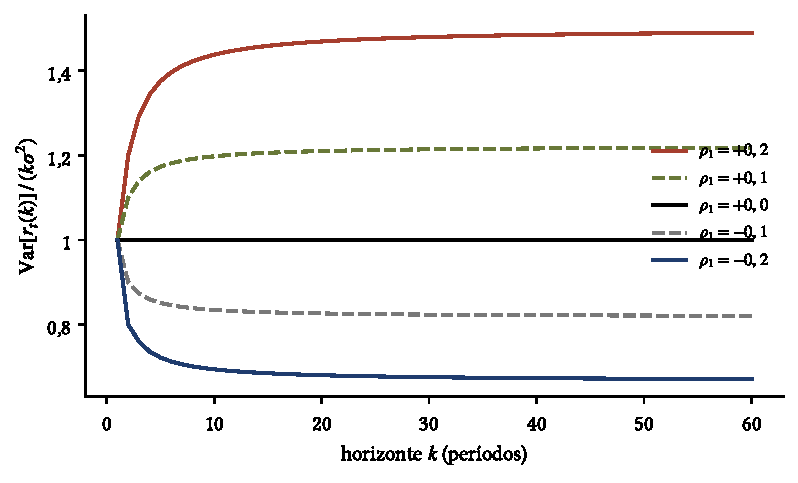
\includegraphics[width=0.72\linewidth]{graficos/cap01_fig_razonvar.pdf}
\caption{Cociente entre la varianza del rendimiento de $k$ períodos y la que predice la regla de la raíz del tiempo ($k\sigma^2$), cuando $\rho_j=\rho_1^{\,j}$. Sin autocorrelación el cociente es 1 en todos los horizontes. Con $\rho_1=0{,}2$ la varianza de largo plazo es un 50\,\% mayor; con $\rho_1=-0{,}2$ es un tercio menor. El límite es $(1+\rho_1)/(1-\rho_1)$.}
\label{fig:razonvar}
\end{figure}


\subsection{Media aritmética y media geométrica}

Con una muestra de $T$ rendimientos simples $R_1,\dots,R_T$ hay dos maneras naturales de promediar:
la media aritmética $A=\frac1T\sum_tR_t$ y la media geométrica $G$, definida por
$(1+G)^T=\prod_t(1+R_t)$, que es la tasa constante que habría producido el mismo valor final.

\begin{proposicion}\label{prop:amgm}
Se cumple $G\le A$, con igualdad si y solo si todos los $R_t$ son iguales. Además, a segundo orden,
\[
  G\approx A-\tfrac12\,s^2,\qquad s^2=\frac1T\sum_{t=1}^T(R_t-A)^2 .
\]
\end{proposicion}

\begin{proof}
Tomamos logaritmos en la definición de $G$ y aplicamos la desigualdad de Jensen a la función cóncava
$\ln$, con pesos $1/T$:
\begin{align*}
  (1+G)^T        &= \prod_{t=1}^T(1+R_t)\\
  T\ln(1+G)      &= \sum_{t=1}^T\ln(1+R_t)\\
  \ln(1+G)       &= \frac1T\sum_{t=1}^T\ln(1+R_t)\\
                 &\le \ln\Bigl(\frac1T\sum_{t=1}^T(1+R_t)\Bigr) && \text{(Jensen)}\\
                 &= \ln(1+A).
\end{align*}
Como el logaritmo es creciente, $G\le A$, con igualdad solo si todos los $R_t$ son iguales.

Para la aproximación, usamos $\ln(1+x)\approx x-\tfrac12x^2$ (Proposición~\ref{prop:taylor}) en ambos
lados de la tercera línea. A la izquierda, $\ln(1+G)\approx G-\tfrac12G^2$. A la derecha,
\begin{align*}
  \frac1T\sum_t\ln(1+R_t) &\approx \frac1T\sum_t\Bigl(R_t-\tfrac12R_t^2\Bigr)\\
                          &= A-\tfrac12\cdot\frac1T\sum_tR_t^2\\
                          &= A-\tfrac12\,(s^2+A^2),
\end{align*}
donde usamos $\frac1T\sum_tR_t^2=s^2+A^2$. Igualando ambos lados:
\begin{align*}
  G-\tfrac12G^2 &\approx A-\tfrac12A^2-\tfrac12s^2\\
  G             &\approx A-\tfrac12s^2+\tfrac12\,(G^2-A^2)\\
  G             &\approx A-\tfrac12s^2.
\end{align*}
En la última línea eliminamos $\tfrac12(G^2-A^2)$: como $G$ y $A$ difieren en términos de segundo orden,
$G^2$ y $A^2$ difieren en términos de tercer orden.
\end{proof}

La diferencia entre ambas medias no es un detalle técnico. La media aritmética es el mejor estimador del
rendimiento \emph{esperado de un período}; la geométrica describe el crecimiento \emph{efectivo} de una
inversión mantenida varios períodos. En activos volátiles, como las acciones mineras, la brecha
$s^2/2$ puede ser de varios puntos porcentuales al año.

\subsection{Rendimientos lognormales}

Un supuesto clásico, que el Capítulo~2 pondrá a prueba con datos, es que el rendimiento logarítmico es
normal.

\begin{proposicion}\label{prop:lognormal}
Si $r_t\sim N(\mu,\sigma^2)$, entonces $1+R_t=e^{r_t}$ tiene distribución lognormal, con
\[
  \E[1+R_t]=e^{\mu+\sigma^2/2},\qquad \operatorname{Mediana}(1+R_t)=e^{\mu},\qquad
  \Var[R_t]=e^{2\mu+\sigma^2}\bigl(e^{\sigma^2}-1\bigr).
\]
\end{proposicion}

\begin{proof}
Calculamos $\E[e^{a\,r_t}]$ para un número real $a$:
\[
  \E[e^{a r_t}]=\int_{-\infty}^{\infty}\frac{1}{\sqrt{2\pi}\,\sigma}
  \exp\Bigl(ax-\frac{(x-\mu)^2}{2\sigma^2}\Bigr)dx .
\]
Completamos el cuadrado en el exponente, escribiendo $ax=a(x-\mu)+a\mu$:
\begin{align*}
  ax-\frac{(x-\mu)^2}{2\sigma^2}
    &= -\frac{(x-\mu)^2-2a\sigma^2(x-\mu)}{2\sigma^2}+a\mu\\
    &= -\frac{(x-\mu)^2-2a\sigma^2(x-\mu)+a^2\sigma^4}{2\sigma^2}+\frac{a^2\sigma^4}{2\sigma^2}+a\mu\\
    &= -\frac{(x-\mu-a\sigma^2)^2}{2\sigma^2}+a\mu+\frac{a^2\sigma^2}{2}.
\end{align*}
Sustituyendo en la integral:
\begin{align*}
  \E[e^{a r_t}]
    &= e^{a\mu+a^2\sigma^2/2}\int_{-\infty}^{\infty}\frac{1}{\sqrt{2\pi}\,\sigma}
       \exp\Bigl(-\frac{(x-\mu-a\sigma^2)^2}{2\sigma^2}\Bigr)dx\\
    &= e^{a\mu+a^2\sigma^2/2}\cdot1\\
    &= e^{a\mu+a^2\sigma^2/2},
\end{align*}
porque la integral es la de una densidad $N(\mu+a\sigma^2,\sigma^2)$. Con $a=1$ y $a=2$:
\begin{align*}
  \E[1+R_t]     &= \E[e^{r_t}] = e^{\mu+\sigma^2/2},\\
  \E[(1+R_t)^2] &= \E[e^{2r_t}] = e^{2\mu+2\sigma^2}.
\end{align*}
Para la varianza:
\begin{align*}
  \Var[R_t] &= \Var[1+R_t]\\
            &= \E[(1+R_t)^2]-\bigl(\E[1+R_t]\bigr)^2\\
            &= e^{2\mu+2\sigma^2}-e^{2\mu+\sigma^2}\\
            &= e^{2\mu+\sigma^2}\bigl(e^{\sigma^2}-1\bigr).
\end{align*}
Por último, la mediana se conserva por transformaciones crecientes: como la mediana de $r_t$ es $\mu$, la
de $e^{r_t}$ es $e^{\mu}$.
\end{proof}

La proposición muestra que la media de los rendimientos simples supera a la mediana en el factor
$e^{\sigma^2/2}$: la distribución de $R_t$ es asimétrica a la derecha aunque la de $r_t$ sea simétrica.
Es la versión poblacional de la Proposición~\ref{prop:amgm}. La Figura~\ref{fig:lognormal} muestra ambas cosas: al crecer $\sigma$ la densidad se vuelve más asimétrica, y la media se aleja de la mediana.
\begin{figure}[ht]
\centering
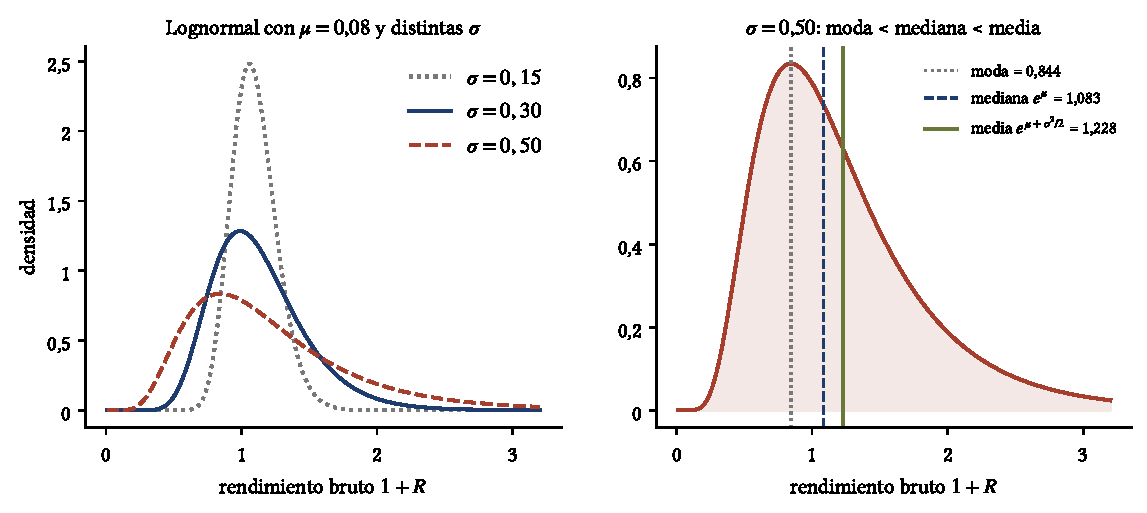
\includegraphics[width=\linewidth]{graficos/cap01_fig_lognormal.pdf}
\caption{Distribución lognormal del rendimiento bruto $1+R=e^{r}$ con $r\sim N(\mu,\sigma^2)$. Izquierda: con más volatilidad la densidad se aplana y se alarga hacia la derecha; la masa se desplaza a valores bajos, pero la cola derecha se extiende. Derecha: con $\sigma=0{,}50$ la moda ($e^{\mu-\sigma^2}$), la mediana ($e^{\mu}$) y la media ($e^{\mu+\sigma^2/2}$) quedan claramente separadas (Proposición~\ref{prop:lognormal}).}
\label{fig:lognormal}
\end{figure}


% ---------------------------------------------------------------------
\section{Datos reales: fuentes, calendarios y sincronización}\label{sec:datos}
% ---------------------------------------------------------------------

\subsection{Fuentes usadas en este capítulo}

\begin{table}[ht]
\centering\footnotesize
\begin{tabularx}{\linewidth}{@{}lXlrll@{}}
\toprule
Serie & Descripción & Fuente & $n$ & Primer dato & Último dato \\
\midrule
\texttt{PD38026MD} & Índice S\&P/BVL Perú General (soles) & BCRPData & 3013 & 14\,794,32 & 54\,971,46 \\
\texttt{PD04638PD} & Tipo de cambio interbancario, venta (S/ por US\$) & BCRPData & 2952 & 2,9830 & 3,4487 \\
\texttt{BAP} & Credicorp Ltd. (NYSE, dólares) & Yahoo Finance & 2981 & 160,18 & 347,93 \\
\texttt{SCCO} & Southern Copper Corp. (NYSE, dólares)$^{a}$ & Yahoo Finance & 2981 & 26,09 & 167,27 \\
\texttt{BVN} & Cía. de Minas Buenaventura (NYSE, ADR) & Yahoo Finance & 2981 & 9,56 & 27,99 \\
\texttt{EPU} & iShares MSCI Peru ETF (dólares) & Yahoo Finance & 2981 & 31,96 & 80,41 \\
\texttt{\^{}GSPC} & Índice S\&P 500 & Yahoo Finance & 2981 & 2\,058,90 & 7\,376,86 \\
\texttt{PEN=X} & Tipo de cambio USD/PEN, último dato del mes & Yahoo Finance & 144 & 2,9930 & 3,4398 \\
\bottomrule
\end{tabularx}
\caption{Series del Capítulo 1 (archivos de \texttt{datos/peru/}). El primer dato es del 31 de diciembre
de 2014 en todas las series; el último, del 5 de noviembre de 2026 (BCRP), del 6 de noviembre de 2026
(acciones e índices de Yahoo) y del 9 de noviembre de 2026 (\texttt{PEN=X}). Descarga: 8 y 9 de noviembre
de 2026. Para las acciones se guardan el cierre y el cierre ajustado. $^{a}$Cierre ya ajustado por los
dividendos en acciones de 2024--2026, que Yahoo registra como desdoblamientos.}
\label{tab:fuentes1}
\end{table}

Los metadatos que devuelve la API del BCRP describen \texttt{PD04638PD} como ``Tipo de cambio -- TC
Interbancario (S/ por US\$) -- Venta''. El índice de la BVL se toma del BCRP y no de Yahoo Finance porque
el símbolo \texttt{\^{}SPBLPGPT} ya no devuelve datos en Yahoo. Al revisar las series aparecieron tres
problemas que se tratan en los ejercicios: (i) el 21 de junio de 2024 el BCRP registra el índice en
22\,521,03, entre 29\,857,57 y 30\,058,66, un dato claramente erróneo que se elimina; (ii) hasta 2020 el
BCRP repite el valor del día anterior en los feriados peruanos (54 rendimientos exactamente iguales a cero),
y desde 2021 los deja como ``n.d.''; (iii) Yahoo Finance registra dos veces el dividendo de Credicorp de
abril de 2020 (Ejercicio~\ref{ej:dividendos}).

\subsection{Problemas prácticos que hay que resolver antes de modelar}

\paragraph{Calendarios de negociación distintos.} La BVL y la Bolsa de Nueva York no cierran los mismos
días: la BVL cierra en feriados peruanos (por ejemplo, el 28 y 29 de julio) y Nueva York en feriados
estadounidenses (por ejemplo, el Día de Acción de Gracias). El BCRP publica el tipo de cambio en días
hábiles del Perú. Al unir series hay dos alternativas: (i) quedarse solo con las fechas comunes
(\emph{intersección}), que pierde observaciones pero no inventa datos; o (ii) completar los faltantes con
el último precio conocido (\emph{arrastre hacia adelante}), que conserva fechas pero genera rendimientos
iguales a cero el día del feriado y un rendimiento acumulado al día siguiente. La segunda opción reduce
artificialmente la varianza diaria y sesga las correlaciones. En este libro usaremos la intersección,
salvo que se indique lo contrario.

\paragraph{Horarios de cierre.} Aunque dos series tengan la misma fecha, sus cierres pueden ocurrir a
horas distintas. El tipo de cambio interbancario del BCRP corresponde al cierre del mercado cambiario
local, que no coincide con el cierre de la Bolsa de Nueva York. Esta asincronía tiene poco efecto en
rendimientos mensuales, pero en datos diarios puede inducir correlaciones rezagadas espurias.

\paragraph{Precios ajustados que cambian.} Cada nuevo dividendo modifica \emph{toda} la historia de
precios ajustados anterior (Proposición~\ref{prop:ajuste}). Por eso dos descargas en fechas distintas
dan niveles de precios ajustados diferentes, aunque los rendimientos sean los mismos. Siempre guardamos
una copia de los datos descargados (carpeta \texttt{datos/}) y registramos la fecha de descarga.

\paragraph{Errores y valores extremos.} Las series públicas contienen ocasionalmente precios repetidos,
días sin negociación registrados con volumen cero o saltos que corresponden a eventos corporativos. Un
rendimiento diario extremo debe verificarse antes de eliminarlo: en finanzas, los valores extremos suelen
ser información (Capítulo~2), no errores.

% ---------------------------------------------------------------------
\section{Ejercicios resueltos}
% ---------------------------------------------------------------------

\begin{ejresuelto}{Dividendos de Credicorp: precio de cierre frente a precio ajustado}\label{ej:dividendos}
\enunciado Con los precios diarios de Credicorp (\texttt{BAP}) desde 2015: (a) identifique las fechas
ex-dividendo a partir del cociente entre el precio ajustado y el de cierre; (b) recupere el monto de cada
dividendo con la ecuación \eqref{eq:factor} y verifique la Proposición~\ref{prop:ajuste}; (c) compare el
rendimiento acumulado con precios de cierre y con precios ajustados y explique la diferencia.

\solucion
\paso{Paso 1. Idea.} Sea $c_t=P^a_t/P_t$ el cociente entre el precio ajustado y el de cierre. Por la regla
de ajuste, $c_t$ es constante entre dos eventos y salta en cada fecha ex-dividendo:
\begin{align*}
  c_{t-1} &= c_t\,f_t\\
  f_t     &= \frac{c_{t-1}}{c_t}\\
  1-\frac{D_t}{P_{t-1}} &= \frac{c_{t-1}}{c_t} && \text{(por \eqref{eq:factor})}\\
  D_t     &= \Bigl(1-\frac{c_{t-1}}{c_t}\Bigr)P_{t-1}.
\end{align*}
\paso{Paso 2. Verificación.} Con $D_t$ recuperado se calculan, en cada fecha ex-dividendo,
\begin{align*}
  R^{\mathrm{tot}}_t       &= \frac{P_t+D_t}{P_{t-1}}-1,\\
  R^{a}_t                  &= \frac{P^{a}_t}{P^{a}_{t-1}}-1,\\
  R^{a}_t-R^{\mathrm{tot}}_t &= \frac{d_t}{1-d_t}\,R^{\mathrm{tot}}_t,
\end{align*}
y se comprueba que la última igualdad (Proposición~\ref{prop:ajuste}) se cumple.

\paso{Paso 3. Cálculo.} Los programas detectan los saltos de $c_t$ mayores que $10^{-4}$, recuperan
$D_t$ y $d_t$, verifican \eqref{eq:difajuste} y calculan el rendimiento acumulado.

\codigoweb{cap01_ej01}
\salidaR{cap01_ej01_R.txt}
\lectura{cap01_ej01}

\RvsPy Ambos lenguajes dan los mismos 17 eventos y los mismos montos. La diferencia de $1{,}41\times
10^{-6}$ fuera de los eventos no es un error de la regla de ajuste: proviene de que el precio ajustado
se guardó con cuatro decimales.

\paso{Paso 4. Comparación con los dividendos anunciados.} La página de relación con inversionistas de
Credicorp publica el monto en dólares de cada dividendo. La Tabla~\ref{tab:divbap} compara los que
figuran ahí con los recuperados.

\begin{table}[H]
\centering\small
\begin{tabular}{@{}lrrl@{}}
\toprule
Fecha ex (Yahoo) & $D_t$ recuperado & Anunciado (US\$) & Fecha de registro \\
\midrule
17-abr-2015 & 2,187 & 2,1900 & 21-abr-2015 \\
14-abr-2016 & 2,316 & 2,3200 & 18-abr-2016 \\
08-abr-2020 & 8,803 & \multirow{2}{*}{8,8026} & \multirow{2}{*}{13-abr-2020} \\
09-abr-2020 & 8,803 & & \\
14-set-2021 & 1,209 & 1,2104 & 15-set-2021 \\
19-may-2022 & 3,994 & 3,9936 & 20-may-2022 \\
18-may-2023 & 6,775 & 6,7749 & 19-may-2023 \\
17-may-2024 & 9,288 & 9,2875 & 20-may-2024 \\
23-set-2024 & 2,917 & 2,9167 & 23-set-2024 \\
19-may-2025 & 11,011 & 11,0162 & 19-may-2025 \\
18-may-2026 & 14,276 & 14,6379 & 18-may-2026 \\
\bottomrule
\end{tabular}
\caption{Dividendos de Credicorp: montos recuperados del precio ajustado y montos anunciados por la
empresa (que los declara en soles y publica su equivalente en dólares). Los años 2017--2019 no figuran en
la página consultada.}
\label{tab:divbap}
\end{table}

Los montos coinciden hasta el redondeo, con dos excepciones. En 2026 Yahoo usa un monto en dólares
menor (14,276 frente a 14,638), probablemente por convertir los soles con otro tipo de cambio. En 2020 la
empresa pagó \emph{un} dividendo de S/\,30 (US\$\,8,8026), pero Yahoo lo registra dos veces, el 8 y el 9 de
abril: el precio ajustado anterior a esa fecha está multiplicado por un factor de más, $0{,}9335$, y el
rendimiento total del período queda sobrestimado. Lo mismo podría ocurrir con los dos registros
consecutivos de abril de 2017 (0,378 y 3,738), que no se pudieron contrastar.

\begin{figure}[H]
\centering
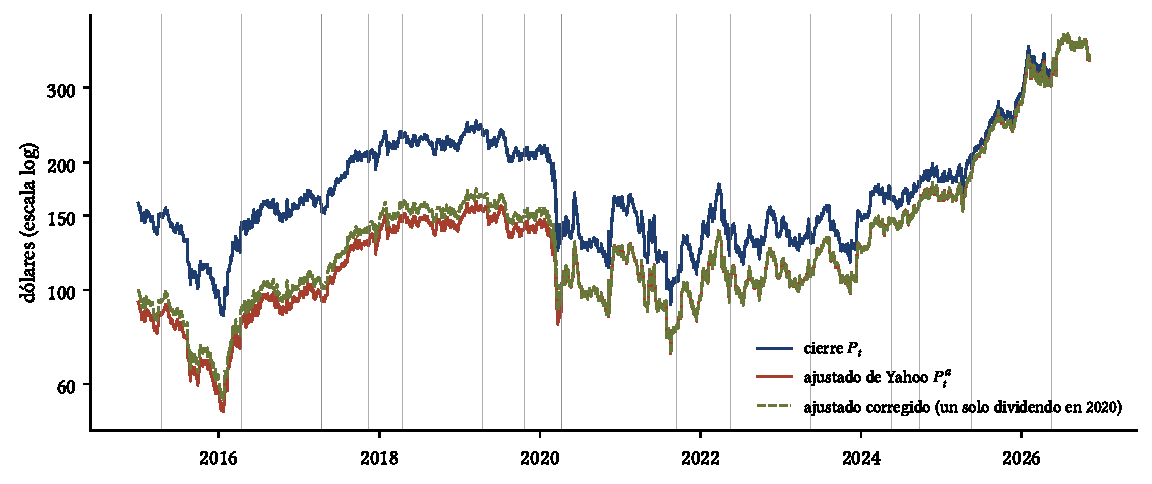
\includegraphics[width=\linewidth]{graficos/cap01_fig_dividendos.pdf}
\caption{Credicorp (\texttt{BAP}), 2015--2026: precio de cierre, precio ajustado de Yahoo Finance y
precio ajustado corregido (un solo dividendo en 2020), en escala logarítmica. Las líneas verticales marcan
las fechas ex-dividendo. Las tres series coinciden después del último dividendo (18 de mayo de 2026).}
\label{fig:divbap}
\end{figure}

\begin{conclusion}
El cociente $c_t$ recupera exactamente los dividendos y la Proposición~\ref{prop:ajuste} se cumple con
error de $3\times10^{-16}$. Sin dividendos, la acción rindió 117,2\,\% entre diciembre de 2014 y noviembre
de 2026 (6,8\,\% anual); con los dividendos reinvertidos rindió 247,0\,\% (11,1\,\% anual). Los dividendos
explican, por tanto, cerca de 4,3 puntos de rentabilidad anual. Si se usa sin revisar el precio ajustado
de Yahoo, el rendimiento acumulado sería 271,8\,\%: un error de descarga de 25 puntos.
\end{conclusion}
\end{ejresuelto}

\begin{ejresuelto}{Rendimientos simples y logarítmicos del mercado peruano y del S\&P 500}\label{ej:logsimple}
\enunciado Con el índice S\&P/BVL Perú General y el S\&P 500: (a) calcule los rendimientos diarios
simples y logarítmicos; (b) verifique que $r_t\le R_t$ en todas las fechas y encuentre el día con mayor
diferencia; (c) agregue a rendimientos mensuales y anuales de dos formas: sumando logaritmos y
multiplicando rendimientos brutos, y compruebe que coinciden (Proposiciones~\ref{prop:multi}
y~\ref{prop:aditiva}).

\solucion
\paso{Paso 1. Datos.} Usamos el índice de la BVL que publica el BCRP (\texttt{PD38026MD}), tras eliminar
el dato erróneo del 21 de junio de 2024, y el S\&P 500 de Yahoo Finance. Si no se elimina ese dato, la
serie muestra un rendimiento logarítmico de $-28{,}2$\,\% seguido de otro de $+28{,}9$\,\%, que dominarían
cualquier estadístico.

\paso{Paso 2. Qué esperar.} Como $r_t=\ln(1+R_t)$ y $\ln(1+x)\le x$, la diferencia
\begin{align*}
  R_t-r_t &= R_t-\ln(1+R_t)\\
          &= \tfrac12R_t^2-\tfrac13R_t^3+\cdots
\end{align*}
es siempre no negativa y crece con $|R_t|$: la mayor diferencia debe aparecer en el día de mayor
movimiento.

\codigoweb{cap01_ej02}
\salidaR{cap01_ej02_R.txt}
\lectura{cap01_ej02}

\RvsPy En R se agrupa con \texttt{tapply} y \texttt{format(fecha, "\%Y-\%m")}; en Python con
\texttt{pd.Grouper}. Las diferencias entre la suma de logaritmos y el logaritmo del producto son del orden
de $10^{-15}$ en ambos: son errores de redondeo de la aritmética de punto flotante, no diferencias de
método.

\begin{figure}[H]
\centering
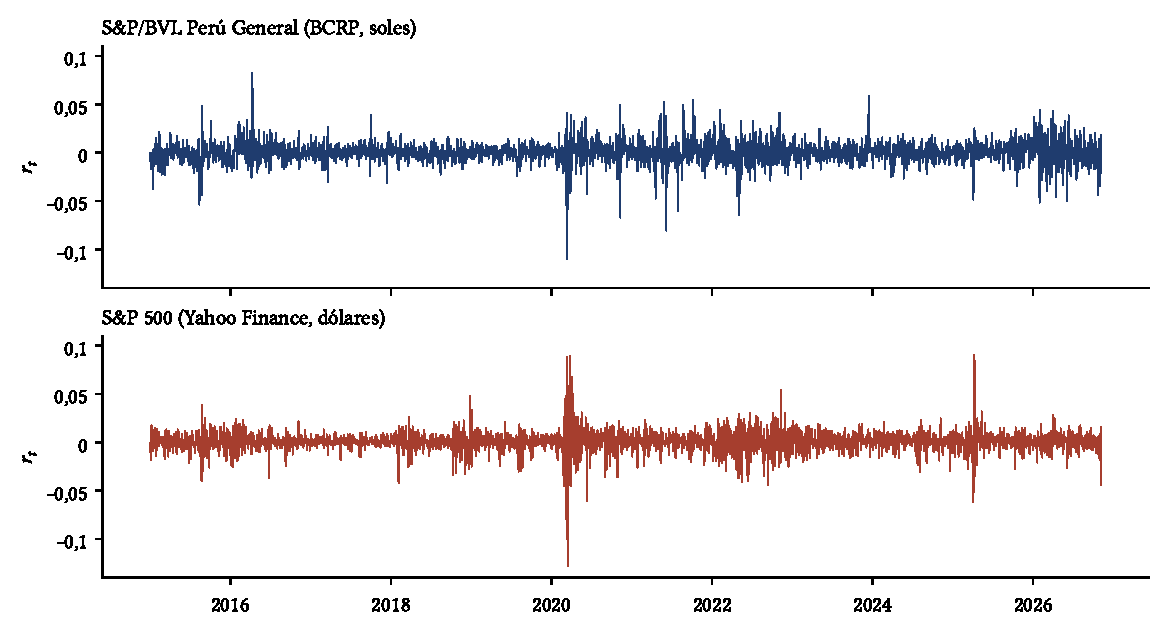
\includegraphics[width=\linewidth]{graficos/cap01_fig_logsimple.pdf}
\caption{Rendimientos logarítmicos diarios del índice S\&P/BVL Perú General (BCRP) y del S\&P 500
(Yahoo Finance), enero de 2015 a noviembre de 2026.}
\label{fig:logsimple-datos}
\end{figure}

\begin{conclusion}
En las 3011 fechas del índice de la BVL y las 2980 del S\&P 500 se cumple $r_t\le R_t$. La mayor
diferencia ocurre en la caída de marzo de 2020: 0,58 puntos porcentuales el 12 de marzo en la BVL
($R_t=-10{,}42$\,\%, $r_t=-11{,}01$\,\%) y 0,78 puntos el 16 de marzo en el S\&P 500. Las Proposiciones
\ref{prop:multi} y \ref{prop:aditiva} se verifican en las 143 agregaciones mensuales y las 12 anuales.
Ambos índices tienen media y volatilidad diarias muy parecidas (0,044\,\% y 1,1\,\%), pero sus
trayectorias anuales difieren mucho: la BVL cayó 33\,\% en 2015 y subió 58\,\% en 2016 y 50\,\% en 2025.
Recuérdese que el índice de la BVL está en soles y el S\&P 500 en dólares.
\end{conclusion}
\end{ejresuelto}

\begin{ejresuelto}{¿Cuánto ganó en soles un inversionista peruano en Southern Copper?}\label{ej:soles}
\enunciado Un inversionista peruano mide su riqueza en soles. (a) Construya el valor en soles de una
acción de \texttt{SCCO} con el tipo de cambio interbancario del BCRP; (b) descomponga el rendimiento
logarítmico anual en soles en la parte de la acción y la parte del tipo de cambio
(Proposición~\ref{prop:moneda}); (c) repita con el tipo de cambio \texttt{PEN=X} de Yahoo Finance y
compare: ¿cambian las conclusiones por la fuente del tipo de cambio?

\solucion
\paso{Paso 1. Planteamiento.} Con $P_t$ el precio ajustado en dólares y $S_t$ el tipo de cambio, el valor
en soles es $V_t=P_tS_t$. Por la Proposición~\ref{prop:moneda}, en cada año
\begin{align*}
  r^{\mathrm{S/}}_t &= \ln V_t-\ln V_{t-1}\\
                    &= (\ln P_t-\ln P_{t-1})+(\ln S_t-\ln S_{t-1})\\
                    &= r^{\$}_t+\Delta\ln S_t .
\end{align*}
Tomamos el último dato disponible de cada fin de año, de 2014 a 2025, y el del 30 de octubre de 2026 como
último corte (fila 2026*), porque \texttt{PEN=X} se guardó con un dato por mes.

\codigoweb{cap01_ej03}
\salidaR{cap01_ej03_R.txt}
\lectura{cap01_ej03}

\RvsPy La función \texttt{ultimo} hace lo mismo en ambos lenguajes: busca el último dato con fecha menor o
igual al corte. Así se resuelve que el 31 de diciembre no sea día hábil en algunos años y que cada serie
tenga su propio calendario.

\begin{figure}[H]
\centering
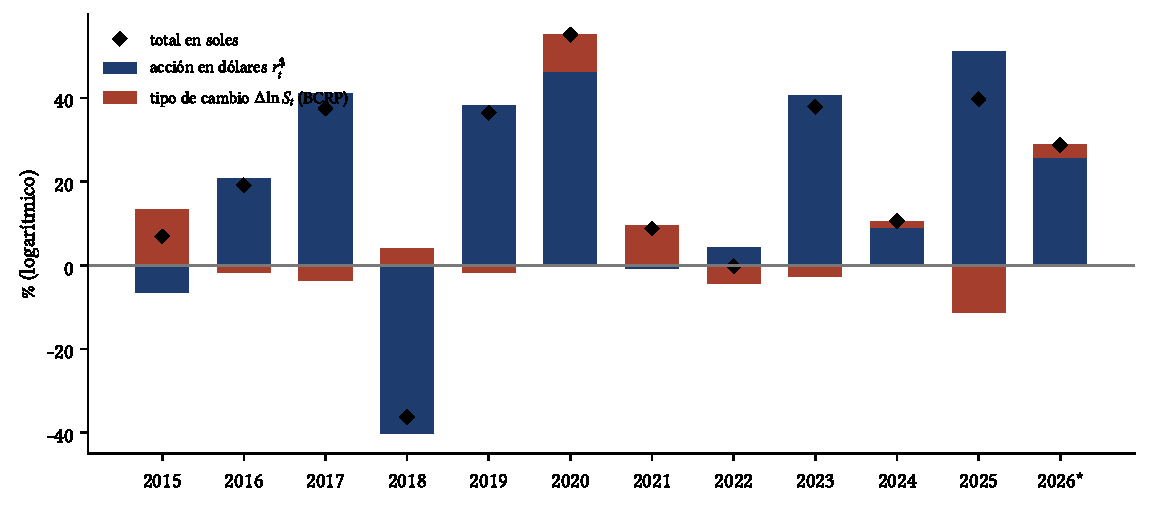
\includegraphics[width=\linewidth]{graficos/cap01_fig_soles.pdf}
\caption{Rendimiento logarítmico anual de \texttt{SCCO} en soles: parte de la acción en dólares y parte
del tipo de cambio interbancario del BCRP. Los rombos marcan el total en soles. 2026*: hasta el 30 de
octubre.}
\label{fig:soles}
\end{figure}

\begin{conclusion}
Entre diciembre de 2014 y octubre de 2026, una acción de Southern Copper rindió 229,7 puntos logarítmicos
en dólares (894\,\% simple) y 244,7 en soles (1055\,\%); los 15 puntos de diferencia son la depreciación
acumulada del sol según el BCRP. El tipo de cambio pesa poco frente a la acción, salvo en años
concretos: en 2015 la depreciación del sol (13,4 puntos) convirtió una pérdida de $-6{,}5$ en dólares en
una ganancia de 6,9 en soles, y en 2025 la apreciación ($-11{,}3$ puntos) le quitó a un inversionista en
soles una cuarta parte de la ganancia. Con \texttt{PEN=X} de Yahoo las conclusiones cualitativas no
cambian, pero las cifras de un año pueden diferir hasta en 2,7 puntos (2015) y el signo de la variación
del tipo de cambio cambia en 2024. Para trabajos sobre el Perú conviene usar el tipo de cambio oficial
del BCRP.
\end{conclusion}
\end{ejresuelto}

\begin{ejresuelto}{Un portafolio de acciones peruanas: suma simple frente a suma logarítmica}\label{ej:portafolio}
\enunciado Considere un portafolio con un tercio del valor en \texttt{BAP}, \texttt{SCCO} y \texttt{BVN},
rebalanceado al inicio de cada mes. (a) Calcule su rendimiento mensual exacto con la
Proposición~\ref{prop:portafolio}; (b) calcule la aproximación $\sum_iw_ir_{i,t}$ y verifique la
Proposición~\ref{prop:logport}; (c) mida el error de aproximación y su relación con la dispersión de los
rendimientos entre las tres acciones; (d) compare con la estrategia sin rebalanceo.

\solucion
\paso{Paso 1. Qué esperar.} Sea $\bar r_t=\sum_iw_ir_{i,t}$. Una expansión de segundo orden de
$e^{r_{i,t}}$ alrededor de $\bar r_t$ da
\begin{align*}
  \sum_iw_ie^{r_{i,t}} &\approx e^{\bar r_t}\sum_iw_i\Bigl[1+(r_{i,t}-\bar r_t)+\tfrac12(r_{i,t}-\bar r_t)^2\Bigr]\\
                       &= e^{\bar r_t}\Bigl[1+\tfrac12\sigma^2_{t}\Bigr],\qquad
                          \sigma^2_t\equiv\sum_iw_i(r_{i,t}-\bar r_t)^2,\\
  r_{p,t}-\bar r_t     &\approx \ln\bigl(1+\tfrac12\sigma^2_t\bigr)\\
                       &\approx \tfrac12\sigma^2_t .
\end{align*}
El error de la aproximación debe ser no negativo (Proposición~\ref{prop:logport}) y aproximadamente igual
a la mitad de la varianza transversal de los rendimientos.

\paso{Paso 2. Datos.} Precios ajustados de Yahoo, con la corrección del dividendo duplicado de Credicorp
(Ejercicio~\ref{ej:dividendos}), y último precio de cada mes. El último mes (noviembre de 2026) es parcial.

\codigoweb{cap01_ej04}
\salidaR{cap01_ej04_R.txt}
\lectura{cap01_ej04}

\RvsPy El producto matricial (\texttt{\%*\%} en R, \texttt{@} en Python) calcula $\sum_iw_iR_{i,t}$ para
todos los meses a la vez. Para la varianza transversal se usa divisor $N$ (no $N-1$) en ambos lenguajes,
porque así está definida $\sigma^2_t$ en el Paso~1.

\begin{figure}[H]
\centering
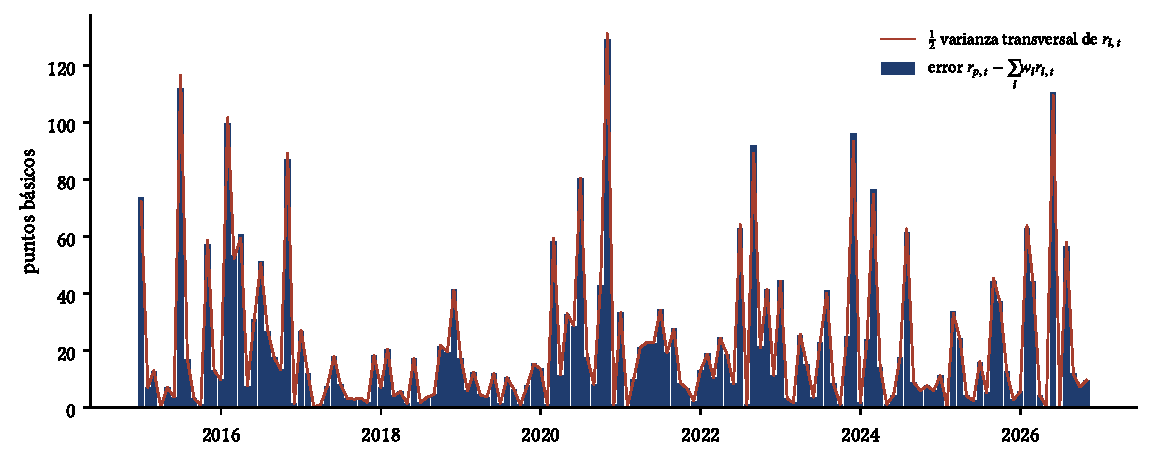
\includegraphics[width=\linewidth]{graficos/cap01_fig_portafolio.pdf}
\caption{Error mensual de aproximar el rendimiento logarítmico del portafolio por
$\sum_iw_ir_{i,t}$ (barras) y la mitad de la varianza transversal de los tres rendimientos (línea), en
puntos básicos.}
\label{fig:portafolio}
\end{figure}

\begin{conclusion}
El error es positivo en los 143 meses, como exige la Proposición~\ref{prop:logport}. En promedio es de
21,7 puntos básicos al mes, pero llega a 129 en noviembre de 2020, cuando las tres acciones se movieron de
forma muy distinta. La regresión del error sobre la varianza transversal da una pendiente de 0,498,
casi exactamente el $\tfrac12$ del Paso~1. Acumulado en 12 años, el error suma 31 puntos logarítmicos:
la aproximación es aceptable para un mes, pero no para medir el rendimiento de largo plazo. El rebalanceo
mensual convirtió un dólar en 6,45; sin rebalancear se habría llegado a 5,39, y Southern Copper habría
pasado a representar el 59\,\% del portafolio.
\end{conclusion}
\end{ejresuelto}

\begin{ejresuelto}{Media aritmética, media geométrica y anualización}\label{ej:anualizar}
\enunciado Con los rendimientos anuales de \texttt{BVN}, \texttt{EPU} y el S\&P 500: (a) calcule las
medias aritmética y geométrica y verifique la aproximación $G\approx A-s^2/2$
(Proposición~\ref{prop:amgm}); (b) anualice la volatilidad diaria con la raíz del tiempo y compárela con
la volatilidad de los rendimientos anuales observados; (c) cuente cuántos días de negociación por año
tiene cada serie y discuta si 252 es adecuado.

\solucion
\paso{Paso 1. Datos.} Usamos los años completos 2015--2025 ($T=11$). Para \texttt{BVN} y \texttt{EPU}
se usa el precio ajustado (rendimiento total); para el S\&P 500, el índice de precios. La volatilidad
diaria se calcula con rendimientos logarítmicos y se anualiza de dos formas: con $\sqrt{252}$ y con la
raíz del número promedio de días observados por año.

\codigoweb{cap01_ej05}
\salidaR{cap01_ej05_R.txt}
\lectura{cap01_ej05}

\RvsPy En la media y la varianza de la parte (a) se usa divisor $T$, como en la
Proposición~\ref{prop:amgm}; en las desviaciones estándar de la parte (b), divisor $T-1$ (\texttt{sd} en
R y \texttt{std} en pandas). Ambos programas dan las mismas cifras.

\begin{figure}[H]
\centering
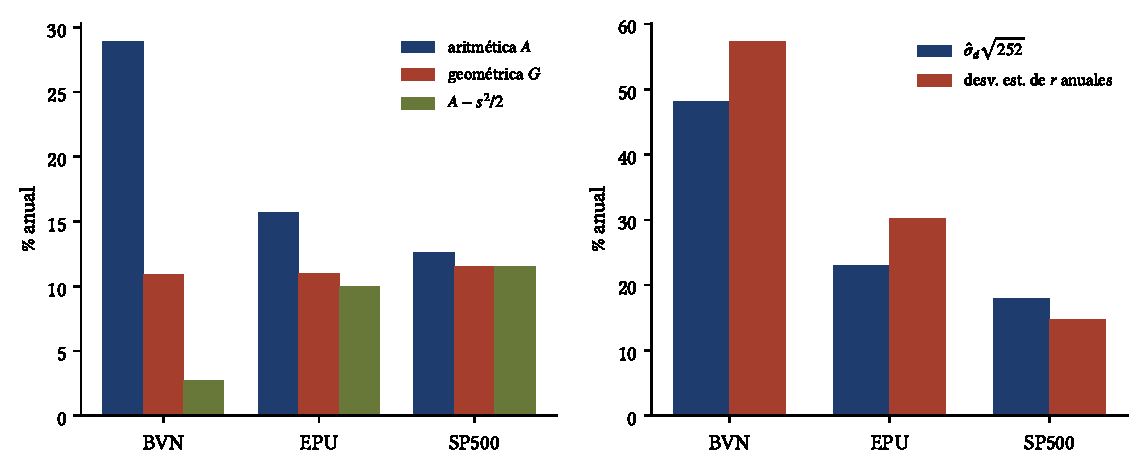
\includegraphics[width=\linewidth]{graficos/cap01_fig_anualizar.pdf}
\caption{Izquierda: medias aritmética y geométrica de los rendimientos anuales 2015--2025 y la
aproximación $A-s^2/2$. Derecha: volatilidad diaria anualizada con $\sqrt{252}$ y desviación estándar
de los rendimientos anuales observados.}
\label{fig:anualizar}
\end{figure}

\begin{conclusion}
(a) En las tres series $G<A$. Para el S\&P 500 la aproximación $G\approx A-s^2/2$ es excelente (11,52
frente a 11,54\,\%) y para \texttt{EPU} razonable (10,00 frente a 11,02\,\%). Para \texttt{BVN} falla
($2{,}72$ frente a $10{,}88$\,\%): con rendimientos anuales de $-55$\,\%, $+164$\,\% o $+148$\,\% los
términos de tercer y cuarto orden que la aproximación omite ya no son pequeños. La media aritmética de
\texttt{BVN} (28,9\,\%) exagera mucho lo que ganó un inversionista que mantuvo la acción (10,9\,\% anual).
(b) Anualizar con $\sqrt{252}$ o con el número de días observados da prácticamente lo mismo. La
volatilidad de los rendimientos anuales observados es mayor que la diaria anualizada en \texttt{BVN} y
\texttt{EPU}, y menor en el S\&P 500. La regla de la raíz del tiempo supone rendimientos independientes;
con solo 11 años, sin embargo, la desviación estándar anual es muy imprecisa. (c) Nueva York tuvo entre 250
y 253 días de negociación por año, así que 252 es adecuado. El BCRP publica 260--261 datos por año hasta
2020, porque repite el valor en los feriados peruanos, y 245--251 desde 2021. Para la BVL, entonces, hay
que contar los días con negociación efectiva y no los días con dato.
\end{conclusion}
\end{ejresuelto}

% ---------------------------------------------------------------------
\section{Ejercicios propuestos}
% ---------------------------------------------------------------------

\begin{enumerate}[label=\textbf{\thechapter.\arabic*},leftmargin=*,itemsep=6pt]
  \item\label{prop:ejsplit} Demuestre la Proposición~\ref{prop:split}: si en $t$ hay un desdoblamiento
  $k\!:\!1$, el precio de cierre cae aproximadamente a $P_{t-1}/k$, y los precios anteriores se
  multiplican por $1/k$, entonces $P^a_t/P^a_{t-1}$ es igual al cociente entre el valor de las $k$
  acciones en $t$ y el de la acción original en $t-1$.
  \textit{Pista: el accionista tiene $k$ acciones en $t$ y una en $t-1$.}

  \item\label{prop:ejasimetria} Demuestre que, para $0<x<1$, la brecha entre el rendimiento simple y el
  logarítmico es mayor para una pérdida que para una ganancia del mismo tamaño:
  $\bigl[-x-\ln(1-x)\bigr]>\bigl[x-\ln(1+x)\bigr]$. Compruebe los valores $0{,}193$ y $0{,}095$ de la
  Figura~\ref{fig:logsimple} para $x=0{,}5$.
  \textit{Pista: estudie $g(x)=-2x-\ln(1-x)+\ln(1+x)$ y su derivada $g'(x)=2x^2/(1-x^2)$.}

  \item\label{prop:ejcorto} Muestre que la desigualdad de la Proposición~\ref{prop:logport} puede
  invertirse con posiciones cortas. \textit{Respuesta: con $w=(2,-1)$, $r_1=0$ y $r_2=\ln 1{,}5$,
  se obtiene $r_p=\ln 0{,}5=-0{,}693<\sum_iw_ir_i=-\ln1{,}5=-0{,}405$.}

  \item Suponga que $\rho_j=\phi^{\,j}$ con $|\phi|<1$ (estructura de un proceso AR(1), Capítulo~6).
  Use la Proposición~\ref{prop:agregmom} para demostrar que
  \[
    \frac{\Var[r_t(k)]}{\sigma^2}=\frac{k(1-\phi^2)-2\phi(1-\phi^k)}{(1-\phi)^2},
  \]
  y que el cociente $\Var[r_t(k)]/(k\sigma^2)$ tiende a $(1+\phi)/(1-\phi)$ cuando $k\to\infty$.

  \item Si $r_t\sim N(\mu,\sigma^2)$, demuestre que $\E[R_t]>\operatorname{Mediana}(R_t)$ siempre que
  $\sigma>0$ y que el cociente $\E[1+R_t]/\operatorname{Mediana}(1+R_t)$ depende solo de $\sigma$.
  \textit{Respuesta: el cociente es $e^{\sigma^2/2}$.}

  \item Demuestre que el rendimiento real logarítmico de $k$ períodos es la suma de los rendimientos
  reales logarítmicos de cada período, y que esa propiedad no se cumple con la aproximación
  $R^{\mathrm{real}}_t\approx R_t-\pi_t$ en rendimientos simples.

  \item \emph{(Con datos.)} Con la inflación mensual de Lima Metropolitana (INEI, disponible también en
  BCRPData), calcule el rendimiento real anual del índice S\&P/BVL Perú General desde 2015 y compárelo
  con el nominal. ¿En qué años el rendimiento nominal fue positivo y el real negativo?

  \item \emph{(Con datos, investigación.)} Repita el Ejercicio~\ref{ej:soles} con \texttt{BVN} y con
  \texttt{EPU}. ¿En qué años la depreciación del sol protegió al inversionista peruano de las pérdidas en
  dólares?

  \item \emph{(Con datos, investigación.)} Identifique los días de 2024 en que la BVL estuvo cerrada y la
  Bolsa de Nueva York abierta, y viceversa. Calcule la correlación diaria entre el índice S\&P/BVL Perú
  General y \texttt{EPU} con intersección de fechas y con arrastre hacia adelante. ¿Cuál es mayor y por
  qué?
\end{enumerate}

% ---------------------------------------------------------------------
\section{Resumen de fórmulas}
% ---------------------------------------------------------------------

\begin{table}[H]
\centering\small
\begin{tabular}{@{}ll@{}}
\toprule
Concepto & Fórmula \\
\midrule
Rendimiento simple & $R_t=P_t/P_{t-1}-1$ \\
Rendimiento total & $R^{\mathrm{tot}}_t=(P_t+D_t)/P_{t-1}-1$ \\
Factor de ajuste por dividendo & $f_t=1-D_t/P_{t-1}$ \\
Rendimiento logarítmico & $r_t=\ln(1+R_t)=\ln P_t-\ln P_{t-1}$ \\
Agregación temporal & $1+R_t(k)=\prod_{j}(1+R_{t-j})$;\quad $r_t(k)=\sum_j r_{t-j}$ \\
Agregación entre activos & $R_{p,t}=\sum_iw_iR_{i,t}$;\quad $r_{p,t}=\ln\sum_iw_ie^{r_{i,t}}$ \\
Rendimiento en soles & $r^{\mathrm{S/}}_t=r^{\$}_t+\Delta\ln S_t$ \\
Rendimiento real & $r^{\mathrm{real}}_t=r_t-\ln(1+\pi_t)$ \\
Varianza de $k$ períodos & $\sigma^2\bigl[k+2\sum_{j=1}^{k-1}(k-j)\rho_j\bigr]$ \\
Media geométrica & $G\approx A-\tfrac12s^2$ \\
Momentos lognormales & $\E[1+R]=e^{\mu+\sigma^2/2}$;\quad $\operatorname{Med}(1+R)=e^{\mu}$ \\
\bottomrule
\end{tabular}
\caption{Fórmulas principales del Capítulo 1.}
\end{table}

\section*{Referencias}
\begin{itemize}[leftmargin=*]
  \item Campbell, J. Y., Lo, A. W. y MacKinlay, A. C. (1997). \emph{The Econometrics of Financial
        Markets}. Princeton University Press. Capítulo 1.
  \item Tsay, R. S. (2010). \emph{Analysis of Financial Time Series} (3.ª ed.). Wiley. Capítulo 1.
  \item Banco Central de Reserva del Perú. \emph{BCRPData: series estadísticas}.
        \url{https://estadisticas.bcrp.gob.pe}.
  \item Instituto Nacional de Estadística e Informática. \emph{Índice de precios al consumidor de Lima
        Metropolitana}. \url{https://www.inei.gob.pe}.
\end{itemize}

% =====================================================================
%  Capítulo 2. Hechos estilizados de los rendimientos financieros
% =====================================================================
\chapter{Hechos estilizados de los rendimientos financieros}\label{cap:hechos}

\section*{Objetivos de aprendizaje}
Al terminar este capítulo, el lector podrá:
\begin{enumerate}[label=\arabic*.,leftmargin=*]
  \item Calcular e interpretar la asimetría y la curtosis muestrales, y derivar su distribución asintótica
        bajo normalidad.
  \item Demostrar y aplicar la prueba de Jarque-Bera, y explicar por qué rechaza casi siempre con datos
        financieros diarios.
  \item Medir el grosor de las colas con el índice de Hill y relacionarlo con la existencia de momentos.
  \item Distinguir entre ausencia de autocorrelación e independencia, usando la autocorrelación de los
        rendimientos, de sus cuadrados y de sus valores absolutos.
  \item Reconocer los artefactos que crean los datos promediados (efecto de Working).
  \item Enunciar los hechos estilizados que los modelos de los capítulos siguientes deben reproducir.
\end{enumerate}

\section*{Motivación}
El 21 de abril de 2020, en plena paralización mundial por la pandemia, el precio spot del petróleo Brent
cayó de 17,36 a 9,12 dólares por barril: un rendimiento logarítmico de $-64$\,\% en un solo día. Al día
siguiente subió 41\,\%. Si los rendimientos diarios del Brent fueran normales, con la volatilidad que
muestran sus casi cuatro décadas de historia, una caída así sería un suceso de 24 desviaciones estándar:
algo que no debería ocurrir ni una sola vez en la vida del universo. Ocurrió, y no fue el único: la
historia del Brent tiene 51 días con movimientos mayores a cuatro desviaciones estándar, cuando la
normal predice menos de uno.

Este capítulo documenta, con datos reales, las regularidades empíricas que comparten los rendimientos de
casi todos los activos financieros: los \emph{hechos estilizados}. No son curiosidades: determinan qué
modelos tienen sentido, qué pruebas estadísticas son válidas y cuánto riesgo se subestima al suponer
normalidad. Cada hecho que documentemos aquí será, más adelante, la motivación de un modelo: el
agrupamiento de volatilidad lleva a los modelos GARCH (Capítulos~8 y~9) y las colas pesadas, a la teoría
de valores extremos del valor en riesgo (Capítulo~13).

\paragraph{Datos del capítulo.} Usamos tres series reales, descargadas el 6 de noviembre de 2026 de los
repositorios públicos \texttt{datasets} de GitHub, que replican automáticamente las fuentes oficiales:
\begin{itemize}[leftmargin=*]
  \item \textbf{Petróleo Brent}, precio spot diario en dólares por barril, del 20 de mayo de 1987 al 3 de
        noviembre de 2026 (9\,122 precios). Fuente original: Administración de Información Energética de
        EE.\,UU. (EIA).
  \item \textbf{S\&P 500 mensual} de la base de datos de Robert Shiller, de enero de 1871 a septiembre de
        2026 (1\,869 precios). Cada dato es el \emph{promedio} de los cierres diarios del mes, un detalle
        decisivo en la Sección~\ref{sec:working}.
  \item \textbf{VIX}, índice de volatilidad de CBOE, diario, de 1990 a septiembre de 2026 (usado en los
        ejercicios propuestos).
\end{itemize}
Los archivos están en \texttt{datos/internacional/} junto con un registro de fuentes. Las aplicaciones
al mercado peruano (índice S\&P/BVL Perú General y acciones mineras) se plantean como ejercicios
propuestos con los datos del Capítulo~\ref{cap:rendimientos}.

% ---------------------------------------------------------------------
\section{Momentos muestrales y la prueba de Jarque-Bera}
% ---------------------------------------------------------------------

Sea $r_1,\dots,r_T$ una muestra de rendimientos logarítmicos, con media $\bar r=\frac1T\sum_tr_t$.

\begin{definicion}[Momentos muestrales centrados]
Para $j\ge 2$, el momento muestral centrado de orden $j$ es $m_j=\frac1T\sum_{t=1}^T(r_t-\bar r)^j$. La
\emph{desviación estándar}, la \emph{asimetría} y la \emph{curtosis} muestrales son
\[
  \hat\sigma=\sqrt{m_2},\qquad \hat S=\frac{m_3}{m_2^{3/2}},\qquad \hat K=\frac{m_4}{m_2^{2}} .
\]
\end{definicion}

La asimetría mide si las desviaciones grandes son más frecuentes de un lado que del otro; un valor
negativo indica que las caídas extremas son más intensas que las subidas extremas. La curtosis mide el
peso de las colas en relación con el centro: para la distribución normal $K=3$, y una curtosis mayor
indica \emph{leptocurtosis}: más observaciones cerca de la media y en las colas, y menos en los
hombros. A $K-3$ se le llama \emph{exceso de curtosis}. La Figura~\ref{fig:momentos} ilustra ambos conceptos con densidades que tienen la misma media y la misma varianza, para que lo único que cambie sea la forma.
\begin{figure}[ht]
\centering
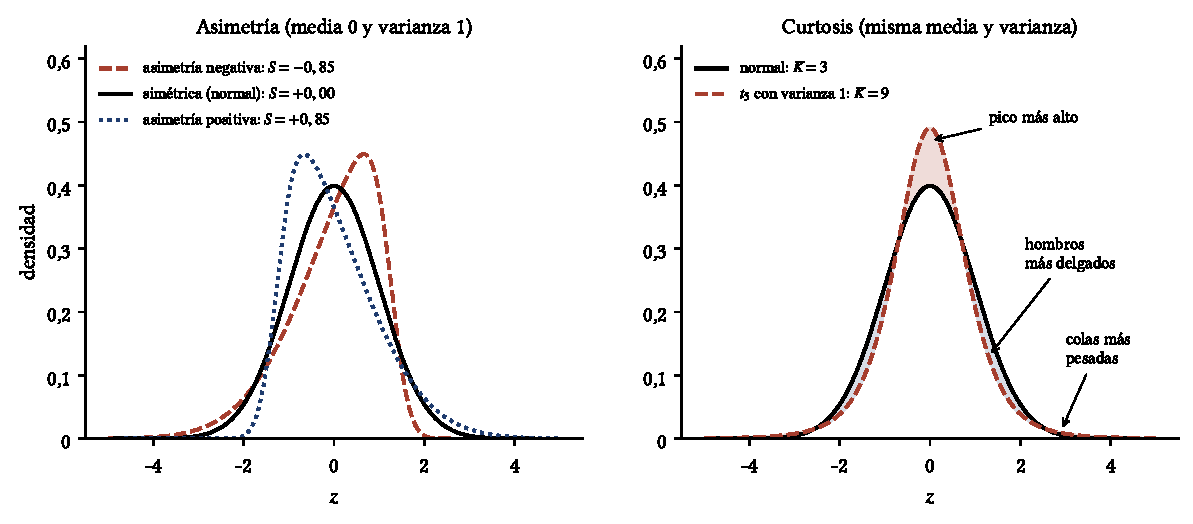
\includegraphics[width=\linewidth]{graficos/cap02_fig_momentos.pdf}
\caption{Izquierda: tres densidades con media 0 y varianza 1 (normal asimétrica). Con asimetría negativa la cola larga está a la izquierda: las caídas extremas son más probables que las subidas extremas. Derecha: normal frente a una $t_5$ reescalada a varianza 1. La $t_5$ tiene más masa en el centro y en las colas (sombreado rojo) y menos en los hombros (sombreado azul): eso es la leptocurtosis.}
\label{fig:momentos}
\end{figure}


\begin{observacion}
Usamos el divisor $T$ (no $T-1$) en todos los momentos, que es la convención de la prueba de Jarque-Bera
y la opción por defecto de \texttt{scipy.stats.skew} y \texttt{scipy.stats.kurtosis}. Otros programas
aplican correcciones de sesgo pequeño; con miles de datos la diferencia es despreciable, pero conviene
saber qué calcula cada función antes de comparar resultados.
\end{observacion}

\begin{teorema}[Distribución asintótica bajo normalidad]\label{teo:jb}
Si $r_1,\dots,r_T$ son independientes e idénticamente distribuidos (i.i.d.) con distribución
$N(\mu,\sigma^2)$, entonces, cuando $T\to\infty$,
\[
  \sqrt T\,\hat S\xrightarrow{d}N(0,6),\qquad \sqrt T\,(\hat K-3)\xrightarrow{d}N(0,24),
\]
y ambos estadísticos son asintóticamente independientes. En consecuencia, el estadístico de
\emph{Jarque-Bera}
\[
  JB=T\left[\frac{\hat S^2}{6}+\frac{(\hat K-3)^2}{24}\right]
\]
converge en distribución a una $\chi^2$ con 2 grados de libertad.
\end{teorema}

\begin{proof}
Como $\hat S$ y $\hat K$ no cambian si los datos se trasladan o se reescalan, basta con considerar
$z_t=(r_t-\mu)/\sigma\sim N(0,1)$. Usaremos los momentos de la normal estándar:
\[
  \E z=\E z^3=\E z^5=\E z^7=0,\qquad \E z^2=1,\qquad \E z^4=3,\qquad \E z^6=15,\qquad \E z^8=105 .
\]
Escribimos $\overline{g}=\frac1T\sum_tg(z_t)$ para cualquier función $g$. Por la ley de los grandes números
$\overline{g}\to\E g(z)$, y por el teorema central del límite $\bar z=O_p(T^{-1/2})$ y
$\overline{z^3}=O_p(T^{-1/2})$.

\emph{Paso 1: asimetría.} Desarrollando el cubo y promediando:
\begin{align*}
  m_3 &= \frac1T\sum_t(z_t-\bar z)^3\\
      &= \overline{z^3}-3\bar z\,\overline{z^2}+3\bar z^2\,\bar z-\bar z^3\\
      &= \overline{z^3}-3\bar z\,\overline{z^2}+2\bar z^3.
\end{align*}
Multiplicando por $\sqrt T$ y usando $\overline{z^2}=1+o_p(1)$ y $\bar z^3=O_p(T^{-3/2})$:
\begin{align*}
  \sqrt T\,m_3 &= \sqrt T\,\overline{z^3}-3\sqrt T\,\bar z\,\overline{z^2}+2\sqrt T\,\bar z^3\\
               &= \sqrt T\,\overline{z^3}-3\sqrt T\,\bar z+o_p(1)\\
               &= \frac1{\sqrt T}\sum_{t=1}^T\bigl(z_t^3-3z_t\bigr)+o_p(1).
\end{align*}
Como $m_2\to1$, $\sqrt T\hat S=\sqrt T\,m_3/m_2^{3/2}$ tiene el mismo límite (teorema de Slutsky). La
variable $u_t=z_t^3-3z_t$ tiene media cero y varianza
\begin{align*}
  \E[u_t^2] &= \E\bigl[z^6-6z^4+9z^2\bigr]\\
            &= 15-6\cdot3+9\cdot1\\
            &= 6 .
\end{align*}
Por el teorema central del límite, $\sqrt T\hat S\xrightarrow{d}N(0,6)$.

\emph{Paso 2: curtosis.} Desarrollando la cuarta potencia y promediando:
\begin{align*}
  m_4 &= \overline{z^4}-4\bar z\,\overline{z^3}+6\bar z^2\,\overline{z^2}-3\bar z^4\\
      &= \overline{z^4}+O_p(T^{-1}),
\end{align*}
porque $\bar z\,\overline{z^3}$ y $\bar z^2$ son $O_p(T^{-1})$. Para el denominador:
\begin{align*}
  m_2      &= \overline{z^2}-\bar z^2\\
           &= 1+\overline{(z^2-1)}+O_p(T^{-1}),\\
  m_2^{-2} &= 1-2\,\overline{(z^2-1)}+O_p(T^{-1}).
\end{align*}
Multiplicando, y usando $\overline{z^4}=3+O_p(T^{-1/2})$ en el término cruzado:
\begin{align*}
  \hat K &= m_4\,m_2^{-2}\\
         &= \overline{z^4}\,\bigl(1-2\,\overline{(z^2-1)}\bigr)+O_p(T^{-1})\\
         &= \overline{z^4}-6\,\overline{(z^2-1)}+O_p(T^{-1})\\
         &= 3+\overline{(z^4-3)}-6\,\overline{(z^2-1)}+O_p(T^{-1}).
\end{align*}
Por tanto,
\begin{align*}
  \sqrt T(\hat K-3) &= \frac1{\sqrt T}\sum_{t=1}^T\bigl[(z_t^4-3)-6(z_t^2-1)\bigr]+o_p(1)\\
                    &= \frac1{\sqrt T}\sum_{t=1}^Tv_t+o_p(1), \qquad v_t=z_t^4-6z_t^2+3 .
\end{align*}
La variable $v_t$ tiene media $3-6+3=0$ y varianza
\begin{align*}
  \E[v_t^2] &= \E\bigl[z^8-12z^6+42z^4-36z^2+9\bigr]\\
            &= 105-12\cdot15+42\cdot3-36\cdot1+9\\
            &= 105-180+126-36+9\\
            &= 24 .
\end{align*}

\emph{Paso 3: independencia y Jarque-Bera.} La covarianza entre $u_t$ y $v_t$ solo contiene momentos
impares:
\begin{align*}
  \E[u_tv_t] &= \E\bigl[(z^3-3z)(z^4-6z^2+3)\bigr]\\
             &= \E\bigl[z^7-9z^5+21z^3-9z\bigr]\\
             &= 0 .
\end{align*}
Por el teorema central del límite multivariado, $\sqrt T(\hat S,\hat K-3)$ converge a una normal bivariada
con matriz de covarianzas $\operatorname{diag}(6,24)$. Los dos componentes estandarizados son normales
estándar independientes en el límite, y la suma de sus cuadrados es una $\chi^2_2$:
\begin{align*}
  JB &= \Bigl(\frac{\sqrt T\,\hat S}{\sqrt6}\Bigr)^2+\Bigl(\frac{\sqrt T\,(\hat K-3)}{\sqrt{24}}\Bigr)^2\\
     &= T\Bigl[\frac{\hat S^2}{6}+\frac{(\hat K-3)^2}{24}\Bigr]\\
     &\xrightarrow{d}\chi^2_2 . && \qedhere
\end{align*}
\end{proof}

\begin{observacion}[Lo que la prueba no dice]
Con $T$ grande, $JB$ rechaza la normalidad ante desviaciones minúsculas. En finanzas el rechazo es tan
seguro que el valor del estadístico importa menos que el diagnóstico: \emph{qué} momento falla y
\emph{por qué}. Además, el Teorema~\ref{teo:jb} supone observaciones independientes. Con datos
financieros, que presentan agrupamiento de volatilidad (Sección~\ref{sec:acf}), la distribución nula de
$JB$ deja de ser exactamente $\chi^2_2$ incluso cuando la distribución marginal fuera normal.
\end{observacion}

% ---------------------------------------------------------------------
\section{Colas pesadas}\label{sec:colas}
% ---------------------------------------------------------------------

\subsection{La distribución $t$ de Student}

La primera alternativa a la normal con colas más pesadas es la $t$ de Student, que usaremos en los
modelos GARCH del Capítulo~9.

\begin{proposicion}\label{prop:curt_t}
Si $X\sim t_\nu$ con $\nu>4$, entonces $\Var(X)=\nu/(\nu-2)$ y su curtosis es
\[
  K=3+\frac{6}{\nu-4}>3 .
\]
Para $\nu\le 4$ el cuarto momento no existe.
\end{proposicion}

\begin{proof}
Representamos $X=Z/\sqrt{W/\nu}$, con $Z\sim N(0,1)$ independiente de $W\sim\chi^2_\nu$. Por
independencia,
\begin{align*}
  \E[X^2] &= \nu\,\E[Z^2]\,\E[W^{-1}] = \nu\,\E[W^{-1}],\\
  \E[X^4] &= \nu^2\,\E[Z^4]\,\E[W^{-2}] = 3\nu^2\,\E[W^{-2}].
\end{align*}
Con la densidad de la $\chi^2_\nu$, $f(w)=w^{\nu/2-1}e^{-w/2}/\bigl(2^{\nu/2}\Gamma(\nu/2)\bigr)$:
\begin{align*}
  \E[W^{-m}] &= \int_0^\infty w^{-m}\,\frac{w^{\nu/2-1}e^{-w/2}}{2^{\nu/2}\Gamma(\nu/2)}\,dw\\
             &= \frac{1}{2^{\nu/2}\Gamma(\nu/2)}\int_0^\infty w^{(\nu/2-m)-1}e^{-w/2}\,dw\\
             &= \frac{2^{\nu/2-m}\,\Gamma(\nu/2-m)}{2^{\nu/2}\,\Gamma(\nu/2)}\\
             &= \frac{\Gamma(\nu/2-m)}{2^m\,\Gamma(\nu/2)},
\end{align*}
que es finita solo si $\nu/2-m>0$. Usando $\Gamma(a+1)=a\,\Gamma(a)$:
\begin{align*}
  \E[W^{-1}] &= \frac{\Gamma(\nu/2-1)}{2\,(\nu/2-1)\,\Gamma(\nu/2-1)} = \frac{1}{\nu-2},\\
  \E[W^{-2}] &= \frac{\Gamma(\nu/2-2)}{4\,(\nu/2-1)(\nu/2-2)\,\Gamma(\nu/2-2)} = \frac{1}{(\nu-2)(\nu-4)}.
\end{align*}
Entonces:
\begin{align*}
  \Var(X) &= \frac{\nu}{\nu-2},\\
  \E[X^4] &= \frac{3\nu^2}{(\nu-2)(\nu-4)},\\
  K       &= \frac{\E[X^4]}{(\Var X)^2}\\
          &= \frac{3\nu^2}{(\nu-2)(\nu-4)}\cdot\frac{(\nu-2)^2}{\nu^2}\\
          &= \frac{3(\nu-2)}{\nu-4}\\
          &= \frac{3(\nu-4)+6}{\nu-4}\\
          &= 3+\frac{6}{\nu-4}.
\end{align*}
Si $\nu\le4$, $\E[W^{-2}]=\infty$ y el cuarto momento no existe.
\end{proof}

La Figura~\ref{fig:tstudent} compara la $t$ con la normal. En escala lineal las diferencias parecen pequeñas; en escala logarítmica se ve lo esencial: la densidad normal cae como una parábola, mientras que la $t$ cae mucho más despacio, y con menos grados de libertad la cola es más pesada.
\begin{figure}[ht]
\centering
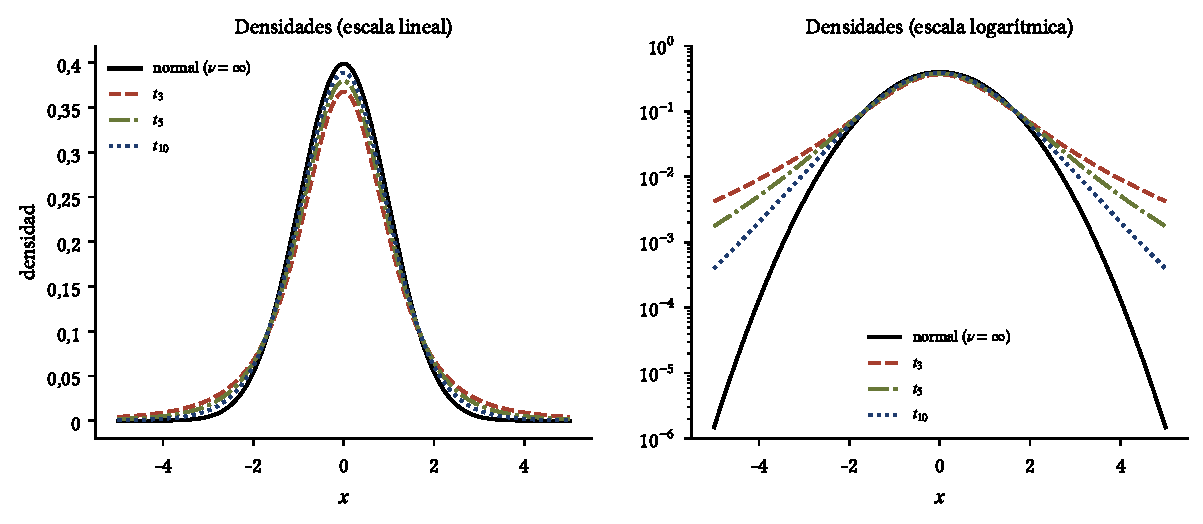
\includegraphics[width=\linewidth]{graficos/cap02_fig_tstudent.pdf}
\caption{Densidades $t$ de Student con $\nu=3,5,10$ y la normal estándar. Izquierda: escala lineal. Derecha: escala logarítmica, donde la normal es una parábola. A cinco unidades del centro, la densidad de la $t_3$ es unas 2\,800 veces la de la normal.}
\label{fig:tstudent}
\end{figure}


\subsection{Colas de tipo Pareto e índice de cola}

Una forma más general de describir colas pesadas es decir que, para pérdidas grandes, la probabilidad de
superar un umbral decae como una potencia y no exponencialmente.

\begin{definicion}[Cola de tipo Pareto]
Una variable $X$ tiene cola derecha de tipo Pareto con \emph{índice de cola} $\alpha>0$ si, para valores
grandes de $x$, $P(X>x)\approx C\,x^{-\alpha}$. Cuanto menor es $\alpha$, más pesada es la cola. La normal
tiene colas que decaen como $e^{-x^2/2}$, más rápido que cualquier potencia: su índice es ``infinito''.
\end{definicion}

\begin{proposicion}[Momentos e índice de cola]\label{prop:momentos_cola}
Si $X\ge u>0$ tiene distribución de Pareto, $P(X>x)=(x/u)^{-\alpha}$ para $x\ge u$, entonces $\E X^k$ es
finito si y solo si $k<\alpha$.
\end{proposicion}

\begin{proof}
La densidad se obtiene derivando la función de distribución:
\begin{align*}
  f(x) &= -\frac{d}{dx}\Bigl(\frac{x}{u}\Bigr)^{-\alpha}\\
       &= \alpha\,u^{\alpha}x^{-\alpha-1}, \qquad x\ge u .
\end{align*}
Entonces
\begin{align*}
  \E[X^k] &= \int_u^\infty x^k\,\alpha u^{\alpha}x^{-\alpha-1}\,dx\\
          &= \alpha u^{\alpha}\int_u^\infty x^{k-\alpha-1}\,dx .
\end{align*}
La integral converge si y solo si $k-\alpha-1<-1$, es decir, $k<\alpha$. En ese caso
\begin{align*}
  \E[X^k] &= \alpha u^{\alpha}\Bigl[\frac{x^{k-\alpha}}{k-\alpha}\Bigr]_u^\infty\\
          &= \alpha u^{\alpha}\cdot\frac{0-u^{k-\alpha}}{k-\alpha}\\
          &= \frac{\alpha\,u^{k}}{\alpha-k}. && \qedhere
\end{align*}
\end{proof}

La consecuencia práctica es fuerte: si los rendimientos tienen índice de cola $\alpha$ entre 2 y 4, la
varianza existe pero la curtosis \emph{poblacional} es infinita. La curtosis muestral sigue siendo un
número finito, pero no converge a nada cuando crece la muestra: su valor depende de cuáles eventos
extremos cayeron en la muestra. Lo comprobaremos con el Brent. La Figura~\ref{fig:pareto} muestra por qué el índice de cola se lee como una pendiente: en escala logarítmica doble, $\ln P(X>x)=\ln C-\alpha\ln x$ es una recta de pendiente $-\alpha$.
\begin{figure}[ht]
\centering
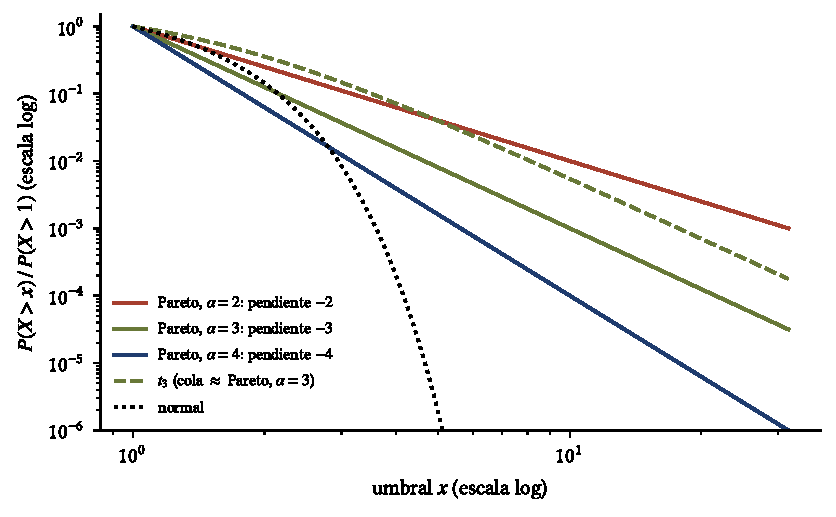
\includegraphics[width=0.75\linewidth]{graficos/cap02_fig_pareto.pdf}
\caption{Probabilidad de superar un umbral, en escala logarítmica doble. Las colas de Pareto son rectas de pendiente $-\alpha$; la $t_3$ termina comportándose como una Pareto con $\alpha=3$; la normal se desploma: su cola decae más rápido que cualquier potencia.}
\label{fig:pareto}
\end{figure}


\begin{proposicion}[Estimador de Hill]\label{prop:hill}
Sean $X_{(1)}\ge X_{(2)}\ge\cdots$ las observaciones ordenadas de mayor a menor. Si las $k$ mayores
observaciones, condicionadas a superar $u=X_{(k+1)}$, siguen una distribución de Pareto con índice
$\alpha$, el estimador de máxima verosimilitud de $\alpha$ es el \emph{estimador de Hill}
\[
  \hat\alpha=\left[\frac1k\sum_{i=1}^k\ln\frac{X_{(i)}}{X_{(k+1)}}\right]^{-1},
\]
con varianza asintótica $\alpha^2/k$.
\end{proposicion}

\begin{proof}
Si $X$ es Pareto por encima de $u$, la variable $Y=\ln(X/u)$ cumple
\begin{align*}
  P(Y>y) &= P\bigl(\ln(X/u)>y\bigr)\\
         &= P\bigl(X>u\,e^{y}\bigr)\\
         &= \Bigl(\frac{u\,e^{y}}{u}\Bigr)^{-\alpha}\\
         &= e^{-\alpha y}:
\end{align*}
es exponencial con tasa $\alpha$ y densidad $\alpha e^{-\alpha y}$. La log-verosimilitud de $k$
observaciones $y_1,\dots,y_k$ y sus derivadas son
\begin{align*}
  \ell(\alpha)   &= \sum_{i=1}^k\ln\bigl(\alpha\,e^{-\alpha y_i}\bigr)\\
                 &= k\ln\alpha-\alpha\sum_{i=1}^ky_i,\\
  \ell'(\alpha)  &= \frac{k}{\alpha}-\sum_{i=1}^ky_i,\\
  \ell''(\alpha) &= -\frac{k}{\alpha^2}.
\end{align*}
Igualando la primera derivada a cero, con $y_i=\ln\bigl(X_{(i)}/X_{(k+1)}\bigr)$:
\begin{align*}
  \frac{k}{\hat\alpha} &= \sum_{i=1}^ky_i\\
  \hat\alpha &= \Bigl[\frac1k\sum_{i=1}^k\ln\frac{X_{(i)}}{X_{(k+1)}}\Bigr]^{-1}.
\end{align*}
La información de Fisher es $-\ell''(\alpha)=k/\alpha^2$, y la varianza asintótica del estimador de máxima
verosimilitud es su inversa:
\begin{align*}
  \Var(\hat\alpha) &\approx \Bigl(\frac{k}{\alpha^2}\Bigr)^{-1}\\
                   &= \frac{\alpha^2}{k}. && \qedhere
\end{align*}
\end{proof}

\begin{observacion}
La elección de $k$ es un compromiso: con $k$ pequeño el estimador usa solo la cola y tiene poco sesgo
pero mucha varianza; con $k$ grande gana precisión pero incluye observaciones donde la aproximación de
Pareto ya no es válida. Por eso se examina $\hat\alpha$ para muchos valores de $k$ (gráfico de Hill) y se
buscan zonas estables.
\end{observacion}

% ---------------------------------------------------------------------
\section{Autocorrelación y dependencia}\label{sec:acf}
% ---------------------------------------------------------------------

\begin{definicion}[Autocorrelación muestral]
La autocorrelación muestral de orden $j$ es
\[
  \hat\rho_j=\frac{\sum_{t=j+1}^T(r_t-\bar r)(r_{t-j}-\bar r)}{\sum_{t=1}^T(r_t-\bar r)^2}.
\]
\end{definicion}

\begin{teorema}[Bartlett]\label{teo:bartlett}
Si $r_t$ es i.i.d. con varianza finita, para cada $m$ fijo el vector
$\sqrt T(\hat\rho_1,\dots,\hat\rho_m)$ converge a una normal con media cero y matriz de covarianzas
identidad. En particular, $\pm1{,}96/\sqrt T$ es una banda de aceptación aproximada al 95\,\% para cada
$\hat\rho_j$, y el estadístico de \emph{Ljung-Box}
\[
  Q(m)=T(T+2)\sum_{j=1}^m\frac{\hat\rho_j^2}{T-j}
\]
converge a una $\chi^2_m$.
\end{teorema}

La demostración usa el teorema central del límite para martingalas y puede consultarse en Brockwell y
Davis (1991, cap.~7). Lo importante aquí es el supuesto: \emph{independencia}, no solo ausencia de
correlación. La siguiente proposición muestra por qué esa diferencia es crucial en finanzas.

\begin{proposicion}[Sin correlación no significa independencia]\label{prop:mds}
Sea $r_t=\sigma_t\varepsilon_t$, donde $\varepsilon_t$ es i.i.d. con media 0 y varianza 1, independiente
de la información pasada $\mathcal F_{t-1}$, y $\sigma_t>0$ depende solo de $\mathcal F_{t-1}$. Entonces:
\begin{enumerate}[label=(\alph*)]
  \item $\Cov(r_t,r_{t-j})=0$ para todo $j\ge1$;
  \item si $\sigma_t^2=\omega+a\,r_{t-1}^2$ con $\omega>0$, $0<a$ y cuarto momento finito, entonces
        $\Cov(r_t^2,r_{t-1}^2)=a\Var(r_{t-1}^2)>0$.
\end{enumerate}
\end{proposicion}

\begin{proof}
(a) Como $\sigma_t$ se conoce en $t-1$ y $\varepsilon_t$ es independiente del pasado,
\begin{align*}
  \E[r_t\mid\mathcal F_{t-1}] &= \E[\sigma_t\varepsilon_t\mid\mathcal F_{t-1}]\\
                              &= \sigma_t\,\E[\varepsilon_t]\\
                              &= 0 .
\end{align*}
Por la ley de esperanzas iteradas, $\E r_t=0$, y como $r_{t-j}$ se conoce en $t-1$:
\begin{align*}
  \Cov(r_t,r_{t-j}) &= \E[r_t\,r_{t-j}]\\
                    &= \E\bigl[\E(r_t\,r_{t-j}\mid\mathcal F_{t-1})\bigr]\\
                    &= \E\bigl[r_{t-j}\,\E(r_t\mid\mathcal F_{t-1})\bigr]\\
                    &= \E[r_{t-j}\cdot0]\\
                    &= 0 .
\end{align*}

(b) Ahora la varianza condicional depende del pasado:
\begin{align*}
  \E[r_t^2\mid\mathcal F_{t-1}] &= \sigma_t^2\,\E[\varepsilon_t^2]\\
                                &= \omega+a\,r_{t-1}^2 .
\end{align*}
Por esperanzas iteradas:
\begin{align*}
  \Cov(r_t^2,r_{t-1}^2)
    &= \E\bigl[r_t^2\,r_{t-1}^2\bigr]-\E\bigl[r_t^2\bigr]\,\E\bigl[r_{t-1}^2\bigr]\\
    &= \E\bigl[r_{t-1}^2\,\E(r_t^2\mid\mathcal F_{t-1})\bigr]
       -\E\bigl[\E(r_t^2\mid\mathcal F_{t-1})\bigr]\,\E\bigl[r_{t-1}^2\bigr]\\
    &= \Cov\bigl(\omega+a\,r_{t-1}^2,\ r_{t-1}^2\bigr)\\
    &= a\,\Var\bigl(r_{t-1}^2\bigr)\\
    &> 0 . && \qedhere
\end{align*}
\end{proof}

El modelo del inciso (b) es el ARCH(1) de Engle (1982), que estudiaremos en el Capítulo~8. La
proposición dice que un mercado puede ser imprevisible en la \emph{dirección} de los precios
(rendimientos sin autocorrelación) y, a la vez, muy previsible en la \emph{magnitud} de los movimientos
(cuadrados autocorrelacionados). Esa es la forma matemática del \emph{agrupamiento de volatilidad}: a
períodos agitados les siguen períodos agitados. La Figura~\ref{fig:arch} lo muestra con una simulación.
\begin{figure}[ht]
\centering
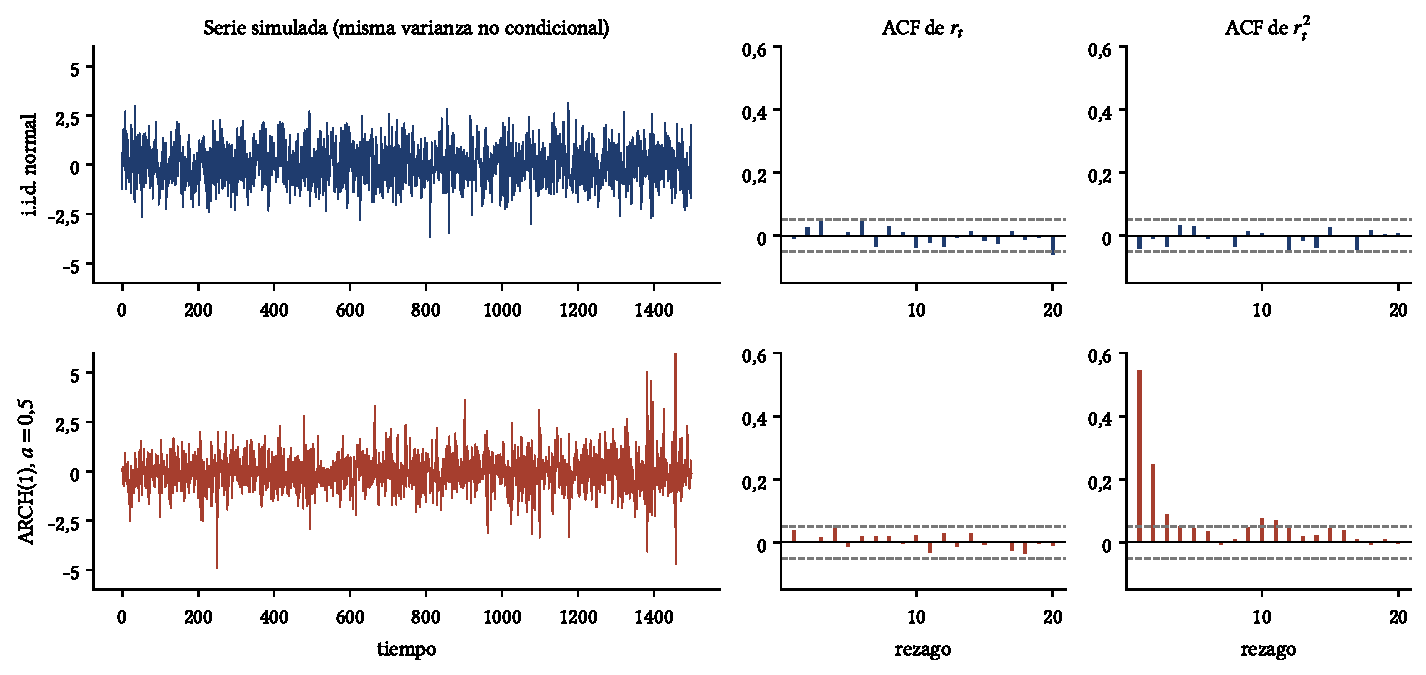
\includegraphics[width=\linewidth]{graficos/cap02_fig_arch.pdf}
\caption{Ruido i.i.d. normal (arriba) frente a un ARCH(1) con $\omega=0{,}5$ y $a=0{,}5$ (abajo), ambos con varianza no condicional 1. Ninguno tiene autocorrelación en $r_t$ (centro), pero solo el ARCH tiene autocorrelación en $r_t^2$ (derecha), y su trayectoria muestra rachas de calma y de turbulencia.}
\label{fig:arch}
\end{figure}


\begin{observacion}[Las bandas de Bartlett con heterocedasticidad]
Si los rendimientos siguen un proceso como el de la Proposición~\ref{prop:mds}, $\hat\rho_j$ sigue
siendo consistente para cero, pero su varianza ya no es $1/T$, sino aproximadamente
$\E[r_t^2r_{t-j}^2]/(T\,\sigma^4)$, que es mayor. Las bandas $\pm1{,}96/\sqrt T$ y la prueba de
Ljung-Box \emph{rechazan demasiado}: detectan autocorrelación donde solo hay volatilidad cambiante. En el
Capítulo~4 corregiremos este problema con errores estándar robustos.
\end{observacion}

% ---------------------------------------------------------------------
\section{Agregación temporal}
% ---------------------------------------------------------------------

Por la Proposición~\ref{prop:aditiva}, el rendimiento logarítmico de $h$ días es la suma de $h$
rendimientos diarios. Si estos tienen varianza finita y dependencia débil, el teorema central del límite
sugiere que la suma se acerca a una normal a medida que $h$ crece: la curtosis de los rendimientos
semanales, mensuales y trimestrales debería ir bajando hacia 3. Este fenómeno se llama
\emph{gaussianidad agregativa}. El índice de cola es la condición clave: si $\alpha>2$, la varianza
existe y el teorema central del límite aplica; si $\alpha<2$, las sumas no se vuelven normales nunca.
La velocidad de convergencia, sin embargo, puede ser lenta, y en muestras finitas unos pocos eventos
extremos pueden dominar los momentos de los rendimientos agregados.

% ---------------------------------------------------------------------
\section{Datos promediados: el efecto de Working}\label{sec:working}
% ---------------------------------------------------------------------

Muchas series publicadas no son precios observados en un instante, sino promedios del período: el
S\&P 500 mensual de Shiller es el promedio de los cierres diarios de cada mes; el tipo de cambio
\emph{promedio} mensual del BCRP también lo es. Working (1960) mostró que promediar crea autocorrelación
donde no la hay.

\begin{proposicion}[Working, 1960]\label{prop:working}
Sea $W(s)$ un movimiento browniano estándar (versión continua de un paseo aleatorio) y
$A_k=\int_{k-1}^{k}W(s)\,ds$ el promedio del período $k$. Los cambios $\Delta A_k=A_k-A_{k-1}$ cumplen
\[
  \Var(\Delta A_k)=\tfrac23,\qquad \Cov(\Delta A_k,\Delta A_{k-1})=\tfrac16,\qquad
  \operatorname{Corr}(\Delta A_k,\Delta A_{k-1})=\tfrac14,
\]
y la autocorrelación de orden $j\ge2$ es cero.
\end{proposicion}

\begin{proof}
Escribimos el cambio de los promedios como una integral de incrementos:
\begin{align*}
  \Delta A_k &= \int_0^1W(k-1+s)\,ds-\int_0^1W(k-2+s)\,ds\\
             &= \int_0^1\bigl[W(k-1+s)-W(k-2+s)\bigr]ds\\
             &= \int_0^1I(s)\,ds,
\end{align*}
donde $I(s)$ es el incremento del browniano en el intervalo $(k-2+s,\,k-1+s]$, de longitud 1. Para un
browniano, la covarianza de dos incrementos es la longitud de la intersección de sus intervalos.

\emph{Varianza.} Los intervalos de $I(s)$ e $I(v)$ se intersecan en una longitud $1-|s-v|$:
\begin{align*}
  \Var(\Delta A_k) &= \int_0^1\!\!\int_0^1\Cov\bigl(I(s),I(v)\bigr)\,ds\,dv\\
                   &= \int_0^1\!\!\int_0^1(1-|s-v|)\,ds\,dv\\
                   &= 1-\int_0^1\!\!\int_0^1|s-v|\,ds\,dv\\
                   &= 1-\tfrac13\\
                   &= \tfrac23 .
\end{align*}
La integral de $|s-v|$ se calcula por simetría, separando las zonas $s<v$ y $s>v$:
\begin{align*}
  \int_0^1\!\!\int_0^1|s-v|\,ds\,dv &= 2\int_0^1\!\!\int_0^v(v-s)\,ds\,dv\\
                                    &= 2\int_0^1\frac{v^2}{2}\,dv\\
                                    &= \int_0^1v^2\,dv\\
                                    &= \tfrac13 .
\end{align*}

\emph{Covarianza de orden 1.} $\Delta A_{k-1}=\int_0^1J(v)\,dv$, con $J(v)$ el incremento en
$(k-3+v,\,k-2+v]$. Ese intervalo y el de $I(s)$ se intersecan en $(k-2+s,\,k-2+v]$, de longitud
$\max(0,v-s)$:
\begin{align*}
  \Cov(\Delta A_k,\Delta A_{k-1}) &= \int_0^1\!\!\int_0^1\max(0,v-s)\,ds\,dv\\
                                  &= \int_0^1\!\!\int_0^v(v-s)\,ds\,dv\\
                                  &= \int_0^1\frac{v^2}{2}\,dv\\
                                  &= \tfrac16 .
\end{align*}
Por tanto,
\begin{align*}
  \operatorname{Corr}(\Delta A_k,\Delta A_{k-1}) &= \frac{1/6}{2/3}\\
                                                 &= \frac14 .
\end{align*}
Para $j\ge2$, los intervalos de $I(s)$ y del incremento de $\Delta A_{k-j}$ no se intersecan, y la
covarianza es cero.
\end{proof}

\begin{observacion}
Con $n$ observaciones discretas por período, Working obtuvo
$\rho_1=(n^2-1)/[2(2n^2+1)]$, que vale $0{,}2492$ para $n=21$ días hábiles por mes y tiende a $1/4$
cuando $n\to\infty$. Un analista que estime un modelo ARMA sobre los rendimientos del S\&P 500 de Shiller
``descubrirá'' una autocorrelación de 0,25 que no dice nada sobre la eficiencia del mercado: es un
artefacto de cómo se construyeron los datos. Siempre hay que saber si una serie es de fin de período o
de promedio del período.
\end{observacion}

% ---------------------------------------------------------------------
\section{Catálogo de hechos estilizados}
% ---------------------------------------------------------------------

Siguiendo a Cont (2001), resumimos los hechos que documentaremos y que los modelos posteriores deben
reproducir.

\begin{table}[ht]
\centering\small
\begin{tabularx}{\linewidth}{@{}>{\raggedright\arraybackslash}p{3.6cm}X>{\raggedright\arraybackslash}p{2.6cm}@{}}
\toprule
Hecho & Descripción & Modelo que lo captura \\
\midrule
Colas pesadas & Curtosis muy superior a 3; índice de cola entre 2 y 5. & $t$ de Student, valores extremos (Cap.~9, 13) \\
Asimetría de pérdidas & Las caídas extremas son mayores que las subidas extremas. & GARCH asimétricos (Cap.~9) \\
Ausencia de autocorrelación lineal & $\hat\rho_j$ de los rendimientos cercanos a cero, salvo en frecuencias muy altas o datos promediados. & Eficiencia de mercado (Cap.~7) \\
Agrupamiento de volatilidad & Autocorrelación positiva y persistente de $r_t^2$ y $|r_t|$. & ARCH/GARCH (Cap.~8) \\
Memoria larga de la volatilidad & La autocorrelación de $|r_t|$ decae muy lentamente. & GARCH integrados, modelos de componentes \\
Gaussianidad agregativa & La distribución se acerca a la normal al aumentar el horizonte. & Teorema central del límite \\
\bottomrule
\end{tabularx}
\caption{Hechos estilizados de los rendimientos financieros.}
\label{tab:hechos}
\end{table}

% ---------------------------------------------------------------------
\section{Ejercicios resueltos}
% ---------------------------------------------------------------------

\begin{ejresuelto}{¿Son normales los rendimientos diarios del petróleo Brent?}\label{ej:brentnormal}
\enunciado Con los precios spot diarios del Brent (EIA, 1987--2026): (a) calcule la media, la desviación
estándar, la asimetría, la curtosis y el estadístico de Jarque-Bera de los rendimientos logarítmicos;
(b) identifique los días más extremos; (c) evalúe la sensibilidad de los momentos a los dos días de abril
de 2020; (d) compare la frecuencia de movimientos mayores a cuatro desviaciones estándar con la que
predice la normal.

\solucion
\paso{Paso 1. Momentos.} Con $T=9\,121$ rendimientos, la media diaria es $0{,}000192$ (unos
$0{,}019$\,\% por día) y la desviación estándar $\hat\sigma=0{,}0270$. La asimetría es $\hat S=-1{,}49$ y
la curtosis $\hat K=55{,}97$: casi diecinueve veces la de una normal.

\paso{Paso 2. Jarque-Bera.} Sustituimos en la fórmula del Teorema~\ref{teo:jb}:
\begin{align*}
  JB &= \frac{T}{6}\Bigl[\hat S^2+\frac{(\hat K-3)^2}{4}\Bigr]\\
     &= \frac{9\,121}{6}\Bigl[(-1{,}4937)^2+\frac{(55{,}966-3)^2}{4}\Bigr]\\
     &= 1\,520{,}17\times\Bigl[2{,}2311+\frac{2\,805{,}40}{4}\Bigr]\\
     &= 1\,520{,}17\times\bigl[2{,}2311+701{,}35\bigr]\\
     &= 1\,520{,}17\times703{,}58\\
     &\approx 1{,}0696\times10^{6}.
\end{align*}
Con todos los decimales se obtiene $1{,}0695\times10^{6}$, el valor de la salida. El valor crítico de la
$\chi^2_2$ al 5\,\% es $5{,}99$: la normalidad se rechaza de forma abrumadora. Casi todo el estadístico
proviene de la curtosis; el término de asimetría aporta solo
\begin{align*}
  \frac{T}{6}\,\hat S^2 &= 1\,520{,}17\times2{,}2311\\
                        &\approx 3\,392 .
\end{align*}

\paso{Paso 3. Días extremos.} Los cinco mayores movimientos son el 21 y el 22 de abril de 2020
($-64{,}4$\,\% y $+41{,}2$\,\%), el 17 de enero de 1991 ($-36{,}1$\,\%, inicio de la operación Tormenta
del Desierto en la Guerra del Golfo), y el 2 y el 31 de marzo de 2020. Cuatro de los cinco ocurren en
el primer semestre de 2020.

\paso{Paso 4. Sensibilidad.} Al quitar solo dos días de 9\,121 (el 0,02\,\% de la muestra), la
curtosis cae de 55,97 a 17,79 y la asimetría de $-1{,}49$ a $-0{,}46$. Un estimador que cambia tanto al
eliminar dos datos no está midiendo una propiedad estable de la distribución. Es la señal empírica de
que el cuarto momento poblacional quizá no exista, lo que verificaremos en el Ejercicio~\ref{ej:hill}.

\paso{Paso 5. Eventos de cuatro sigmas.} Comparamos el número de días con $|z_t|>4$ observado y el que
predice la normal:
\begin{align*}
  \text{días observados}  &= 0{,}005591\times9\,121\\
                          &\approx 51,\\
  \text{días esperados}   &= 2\,\Phi(-4)\times9\,121\\
                          &= 6{,}334\times10^{-5}\times9\,121\\
                          &\approx 0{,}58,\\
  \text{cociente}         &= \frac{0{,}005591}{6{,}334\times10^{-5}}\\
                          &\approx 88 .
\end{align*}
Los movimientos extremos son 88 veces más frecuentes de lo que supone la normal.

\codigoweb{cap02_ej01}
\salidaR{cap02_ej01_R.txt}
\lectura{cap02_ej01}

\RvsPy R no trae funciones de asimetría y curtosis en su instalación base, así que las programamos
directamente desde la definición; Python las toma de \texttt{scipy.stats}. Hay que fijar en Python
\texttt{fisher=False} para obtener la curtosis (y no el exceso de curtosis) y \texttt{ddof=0} en la
desviación estándar para que coincida con $\sqrt{m_2}$. Con esas precauciones, ambas salidas coinciden
en todas las cifras.

\begin{figure}[ht]
\centering
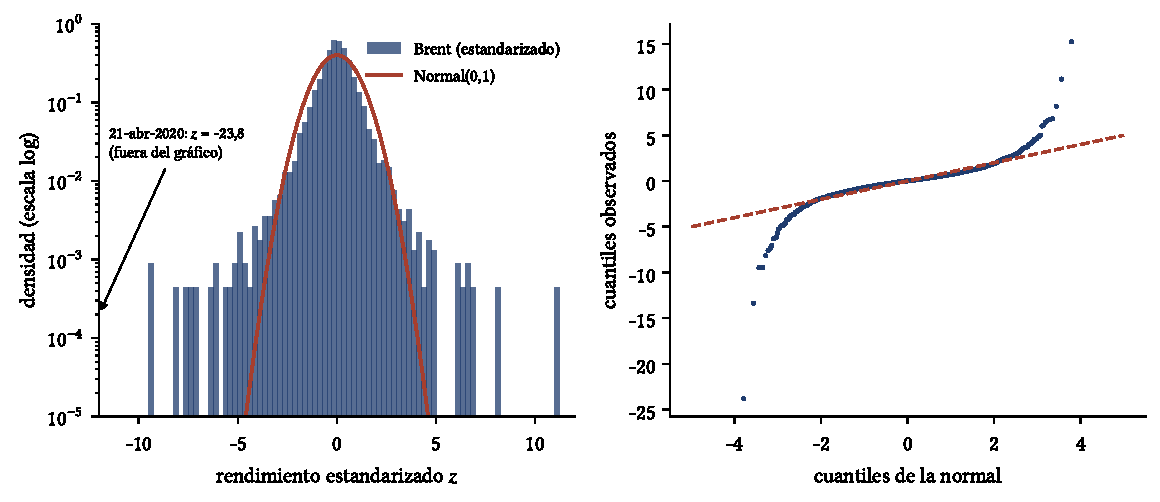
\includegraphics[width=\linewidth]{graficos/cap02_fig_normalidad.pdf}
\caption{Rendimientos diarios estandarizados del Brent, 1987--2026. Izquierda: histograma en escala
logarítmica frente a la densidad normal; la normal es una parábola en esta escala, y los datos tienen
un pico más alto y colas mucho más gruesas. Derecha: gráfico cuantil-cuantil; los puntos se separan de
la recta en ambos extremos, con más fuerza en las pérdidas.}
\label{fig:normalidad}
\end{figure}

\begin{conclusion}
Los rendimientos diarios del Brent no son normales: tienen colas extremadamente pesadas y asimetría
negativa. Un modelo de riesgo basado en la normal subestimaría la frecuencia de movimientos extremos
en un factor cercano a 90. Además, la curtosis muestral es inestable y depende de unos pocos días, por
lo que no debe reportarse sin un análisis de sensibilidad.
\end{conclusion}
\end{ejresuelto}

\begin{ejresuelto}{Rendimientos impredecibles, volatilidad predecible}\label{ej:acf}
\enunciado Con los rendimientos diarios del Brent: (a) calcule las autocorrelaciones de orden 1 a 10 de
$r_t$, $r_t^2$ y $|r_t|$; (b) aplique la prueba de Ljung-Box con $m=10$ y $m=20$; (c) interprete los
resultados a la luz de la Proposición~\ref{prop:mds}.

\solucion
\paso{Paso 1. Banda de referencia.} Con $T=9\,121$, la banda de Bartlett al 95\,\% es
\begin{align*}
  \pm\frac{1{,}96}{\sqrt T} &= \pm\frac{1{,}96}{\sqrt{9\,121}}\\
                            &= \pm\frac{1{,}96}{95{,}50}\\
                            &= \pm0{,}0205 .
\end{align*}

\paso{Paso 2. Rendimientos.} Las diez autocorrelaciones de $r_t$ están entre $-0{,}028$ y $0{,}021$;
la de primer orden es $-0{,}003$. Tres de ellas rozan la banda (rezagos 2, 8 y 10), pero ninguna tiene
importancia económica: una autocorrelación de 0,02 explica el 0,04\,\% de la varianza del día siguiente.

\paso{Paso 3. Cuadrados y valores absolutos.} La autocorrelación de primer orden de $r_t^2$ es $0{,}33$,
dieciséis veces la banda, y la de $|r_t|$ es $0{,}26$. Todas las autocorrelaciones de $|r_t|$ hasta el
rezago 10 están entre 0,18 y 0,26, y la Figura~\ref{fig:acf} muestra que siguen siendo positivas y
significativas más allá del rezago 100: la volatilidad tiene una memoria muy larga.

\paso{Paso 4. Ljung-Box.} Para $|r_t|$, $Q(10)=4\,170{,}8$ y para $r_t^2$, $Q(10)=1\,721{,}3$, frente a un
valor crítico de $\chi^2_{10}$ al 5\,\% de $18{,}3$: rechazo abrumador. Para $r_t$, $Q(10)=25{,}74$
($p=0{,}0041$) también rechaza. Este último resultado debe leerse con cuidado: por la observación que
sigue a la Proposición~\ref{prop:mds}, la prueba de Ljung-Box rechaza en exceso cuando la volatilidad
cambia en el tiempo, que es justamente lo que muestran los pasos~3 y~4. El rechazo para $r_t$ es
compatible con autocorrelaciones verdaderas nulas y volatilidad cambiante; en el Capítulo~4 lo
verificaremos con una versión robusta de la prueba.

\codigoweb{cap02_ej02}
\salidaR{cap02_ej02_R.txt}
\lectura{cap02_ej02}

\RvsPy \texttt{acf()} y \texttt{Box.test()} pertenecen a la instalación base de R; en Python usamos
\texttt{statsmodels}. Las dos funciones de autocorrelación usan el mismo denominador $\sum(r_t-\bar r)^2$
para todos los rezagos, por lo que los valores coinciden. Para el $p$-valor en R calculamos la cola
superior con \texttt{pchisq(..., lower.tail = FALSE)}: la salida por defecto de \texttt{Box.test()}
calcula $1-F(Q)$ y redondea a cero los $p$-valores muy pequeños.

\begin{figure}[ht]
\centering
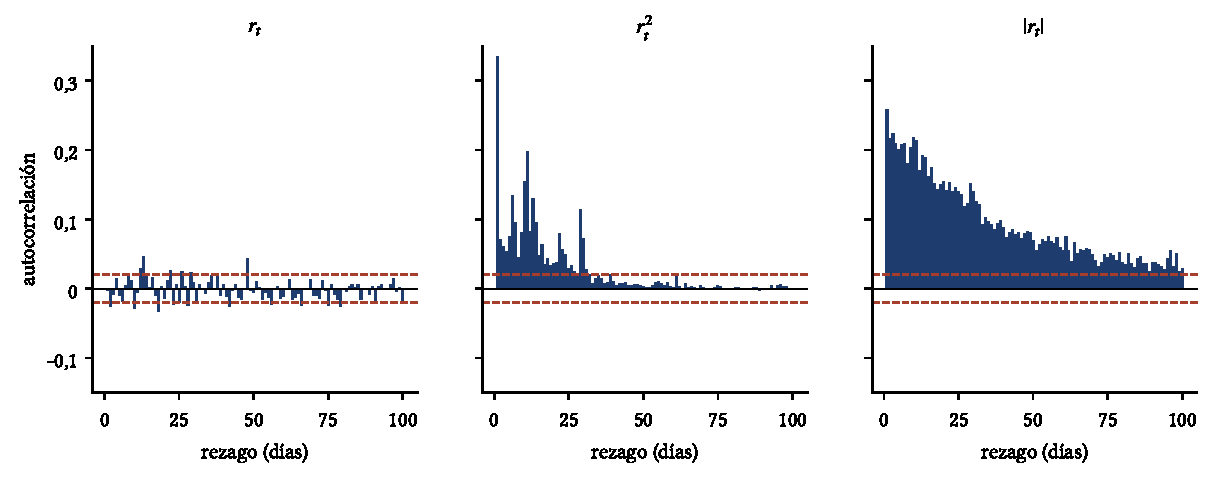
\includegraphics[width=\linewidth]{graficos/cap02_fig_acf.pdf}
\caption{Autocorrelaciones del Brent hasta el rezago 100, con la banda de Bartlett al 95\,\% (líneas
discontinuas). Los rendimientos casi no tienen autocorrelación; sus cuadrados y, sobre todo, sus valores
absolutos tienen autocorrelaciones positivas que decaen muy lentamente.}
\label{fig:acf}
\end{figure}

\begin{conclusion}
El Brent ilustra la Proposición~\ref{prop:mds}: la dirección del precio de mañana es prácticamente
impredecible a partir de los rendimientos pasados, pero su volatilidad es altamente predecible. Este es
el hecho estilizado que motiva los modelos ARCH y GARCH.
\end{conclusion}
\end{ejresuelto}

\begin{ejresuelto}{¿Se vuelven normales los rendimientos al agregarlos?}\label{ej:agregacion}
\enunciado Agregue los rendimientos diarios del Brent en bloques sin traslape de $h=1,5,21,63$ y $126$
días de negociación (aproximadamente día, semana, mes, trimestre y semestre). Para cada horizonte calcule
la desviación estándar, la asimetría, la curtosis y el $p$-valor de Jarque-Bera. ¿Se cumple la
gaussianidad agregativa? ¿Se cumple la regla de la raíz del tiempo?

\solucion
\paso{Paso 1. Tendencia general.} La curtosis cae de 55,97 ($h=1$) a 14,81 ($h=5$), 4,93 ($h=63$) y
3,84 ($h=126$). Con bloques semestrales, Jarque-Bera ya no rechaza la normalidad ($p=0{,}344$), aunque
con solo 72 observaciones la prueba tiene poca potencia.

\paso{Paso 2. Una excepción instructiva.} Con $h=21$ la curtosis \emph{sube} a 24,93. La razón es que,
con 434 observaciones mensuales, un único mes extremo (marzo-abril de 2020) pesa muchísimo en el cuarto
momento. La Figura~\ref{fig:agregacion} muestra que el pico en $h=21$ persiste incluso sin el 21 y el
22 de abril de 2020: no lo producen dos días, sino un período completo de crisis. La convergencia a la
normal existe, pero es lenta y errática cuando las colas son tan pesadas como las del
Ejercicio~\ref{ej:hill}.

\paso{Paso 3. Raíz del tiempo.} Comparamos el cociente de volatilidades con el que predice la regla:
\begin{align*}
  \frac{\hat\sigma_{21}}{\hat\sigma_{1}} &= \frac{0{,}12807}{0{,}027039}\\
                                          &= 4{,}736,\\
  \sqrt{21}                               &= 4{,}583,\\
  \frac{4{,}736}{4{,}583}                 &= 1{,}033 .
\end{align*}
La volatilidad mensual es un 3,3\,\% mayor de lo que predice la regla de la raíz del tiempo, una
diferencia moderada. Por la Proposición~\ref{prop:agregmom}, apunta a una leve autocorrelación positiva
acumulada en los rendimientos diarios, o simplemente al peso de 2020 en una muestra mensual pequeña.

\codigoweb{cap02_ej03}
\salidaR{cap02_ej03_R.txt}
\lectura{cap02_ej03}

\RvsPy La agregación sin traslape se resuelve igual en ambos lenguajes: se descarta el bloque final
incompleto y se ordenan los datos en una matriz de $h$ filas (R, que llena por columnas) o de $h$
columnas (Python, que llena por filas), sumando luego a lo largo del bloque. Confundir el orden de
llenado es un error frecuente que produce sumas de días no consecutivos.

\begin{figure}[ht]
\centering
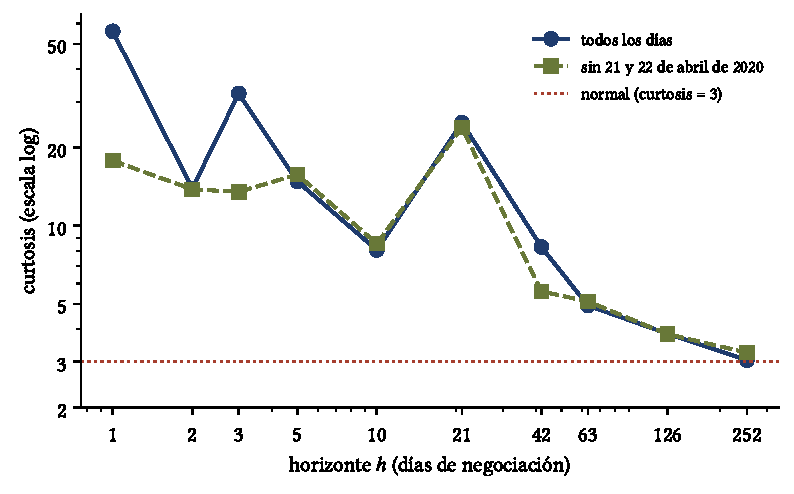
\includegraphics[width=0.8\linewidth]{graficos/cap02_fig_agregacion.pdf}
\caption{Curtosis de los rendimientos del Brent agregados a $h$ días (ambos ejes en escala
logarítmica). La tendencia hacia el valor normal de 3 es clara a partir de $h=42$, pero el camino es
irregular; el pico de $h=21$ refleja la crisis de marzo-abril de 2020.}
\label{fig:agregacion}
\end{figure}

\begin{conclusion}
La gaussianidad agregativa se cumple a horizontes largos, pero no conviene confiar en ella a horizontes
de un mes: la distribución mensual del Brent sigue teniendo colas muy pesadas. Para la gestión de
riesgos a un mes no es seguro suponer normalidad solo porque se trabaja con datos menos frecuentes.
\end{conclusion}
\end{ejresuelto}

\begin{ejresuelto}{Una autocorrelación que no existe: el S\&P 500 mensual de Shiller}\label{ej:working}
\enunciado Con el S\&P 500 mensual de Shiller (1871--2026): (a) calcule las autocorrelaciones de orden 1
a 6 de los cambios logarítmicos mensuales, en la muestra completa y en los tramos 1871--1945 y
1946--2026; (b) compárelas con el valor teórico de Working; (c) concluya si existe evidencia de
predictibilidad en el mercado accionario estadounidense.

\solucion
\paso{Paso 1. Resultado.} La autocorrelación de primer orden es $0{,}274$ en la muestra completa
($T=1\,868$), seis veces la banda de $0{,}045$; Ljung-Box con $m=1$ da $Q=140{,}6$ y $p=1{,}97\times10^{-32}$.
Los rezagos 2 a 6 son pequeños: entre $-0{,}040$ y $0{,}073$.

\paso{Paso 2. Comparación con Working.} El patrón (una autocorrelación cercana a 0,25 en el primer rezago
y casi nada después) es exactamente el de la Proposición~\ref{prop:working}, con valor teórico de
$0{,}2492$ para 21 días hábiles por mes. La Figura~\ref{fig:working} lo confirma con una simulación: un
paseo aleatorio muestreado a fin de mes no muestra autocorrelación, y el mismo paseo promediado dentro de
cada mes muestra una de $0{,}224$ en el primer rezago, muy cerca del valor de los datos.

\paso{Paso 3. Por tramos.} En 1871--1945 la autocorrelación es $0{,}310$ y en 1946--2026, $0{,}213$.
Ambas están cerca de 1/4. Cada estimación tiene un error estándar aproximado de
$1/\sqrt{900}\approx0{,}033$, así que la diferencia de $0{,}097$ entre tramos equivale a unas dos veces su
error estándar ($\approx0{,}047$): una diferencia marginal que no conviene interpretar sin más análisis.

\codigoweb{cap02_ej04}
\salidaR{cap02_ej04_R.txt}
\lectura{cap02_ej04}

\RvsPy El tratamiento de las fechas difiere: en R se filtra con comparaciones lógicas sobre un vector de
clase \texttt{Date}; en Python, la serie indexada por fechas de \texttt{pandas} permite cortes como
\texttt{r[:"1945-12-01"]}, que incluyen ambos extremos. Los resultados coinciden.

\begin{figure}[ht]
\centering
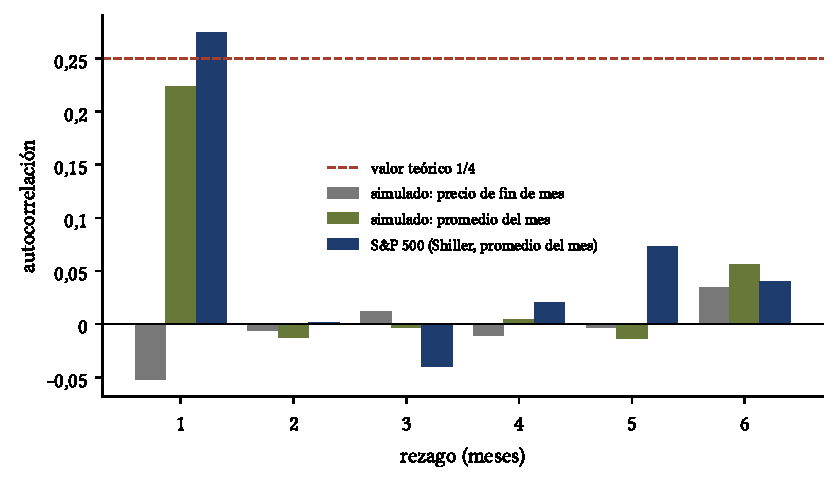
\includegraphics[width=0.82\linewidth]{graficos/cap02_fig_working.pdf}
\caption{Autocorrelaciones de rendimientos mensuales. Un paseo aleatorio simulado no tiene
autocorrelación si se toma el precio de fin de mes (gris), pero sí si se toma el promedio del mes
(verde). El S\&P 500 de Shiller (azul), construido con promedios, reproduce el patrón y se acerca al
valor teórico de 1/4.}
\label{fig:working}
\end{figure}

\begin{conclusion}
La autocorrelación de 0,27 de los rendimientos mensuales de Shiller no es evidencia de que el mercado
estadounidense sea predecible: la explica casi por completo el uso de precios promedio. Antes de
interpretar cualquier autocorrelación, hay que verificar cómo se construyó la serie. La misma advertencia
aplica al tipo de cambio \emph{promedio} mensual que publica el BCRP.
\end{conclusion}
\end{ejresuelto}

\begin{ejresuelto}{¿Qué tan pesadas son las colas del Brent?}\label{ej:hill}
\enunciado Estime el índice de cola del Brent con el estimador de Hill, por separado para las pérdidas
($-r_t$) y para las ganancias ($r_t$), con $k=50,100,200$ y $400$. Construya el gráfico de Hill para
$k$ entre 20 y 900. ¿Existe la varianza? ¿Existe la curtosis?

\solucion
\paso{Paso 1. Estimaciones.} Para las pérdidas, $\hat\alpha$ toma los valores $2{,}52$, $2{,}76$, $2{,}56$
y $2{,}67$; para las ganancias, $2{,}94$, $3{,}30$, $2{,}85$ y $2{,}56$. Los errores estándar
$\hat\alpha/\sqrt k$ van de $0{,}36$ ($k=50$) a $0{,}13$ ($k=400$).

\paso{Paso 2. Intervalos.} Con $k=200$, el intervalo de confianza aproximado al 95\,\% para la cola de
pérdidas es
\begin{align*}
  \hat\alpha\pm1{,}96\,\operatorname{ee}(\hat\alpha) &= 2{,}558\pm1{,}96\times0{,}181\\
                                                     &= 2{,}558\pm0{,}355\\
                                                     &= [2{,}20;\ 2{,}91].
\end{align*}
Está entero por encima de 2 y entero por debajo de 4.

\paso{Paso 3. Interpretación.} Por la Proposición~\ref{prop:momentos_cola}, con $2<\alpha<4$ la varianza
existe pero el cuarto momento no. Esto explica lo que vimos en los ejercicios anteriores: una curtosis
muestral enorme e inestable, que cambia mucho al quitar dos datos (Ejercicio~\ref{ej:brentnormal}) y que
converge lentamente a 3 al agregar (Ejercicio~\ref{ej:agregacion}). La curtosis de 55,97 no es una
``medida'' del riesgo de cola del Brent; el índice de cola sí lo es.

\paso{Paso 4. Asimetría de las colas.} Para $k\le200$ la cola de pérdidas es algo más pesada (menor
$\alpha$) que la de ganancias, en línea con la asimetría negativa; para $k=400$ ambas se igualan.

\codigoweb{cap02_ej05}
\salidaR{cap02_ej05_R.txt}
\lectura{cap02_ej05}

\RvsPy Ambos programas ordenan los datos de mayor a menor (\texttt{sort(..., decreasing = TRUE)} en R y
\texttt{np.sort(...)[::-1]} en Python). Hay que cuidar el índice del umbral: en R, cuya indexación
empieza en 1, el umbral $X_{(k+1)}$ es \texttt{xs[k + 1]}; en Python, que empieza en 0, es
\texttt{xs[k]}. Un error en este índice cambia los resultados sin producir ningún mensaje de error.

\begin{figure}[ht]
\centering
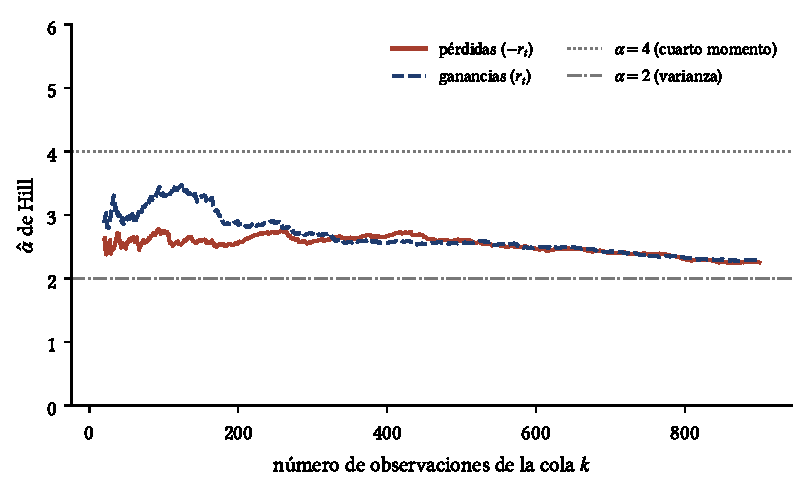
\includegraphics[width=0.82\linewidth]{graficos/cap02_fig_hill.pdf}
\caption{Gráfico de Hill del Brent. Para casi todo el rango de $k$, el índice de cola estimado está entre
2 y 4: la varianza existe, pero el cuarto momento no.}
\label{fig:hill}
\end{figure}

\begin{conclusion}
El índice de cola del Brent está alrededor de 2,5 a 3. La varianza existe, de modo que la volatilidad es
una medida legítima de riesgo, pero el cuarto momento probablemente no, de modo que la curtosis muestral
no debe usarse como medida de riesgo de cola. Para medir riesgos extremos usaremos la teoría de valores
extremos del Capítulo~13.
\end{conclusion}
\end{ejresuelto}

% ---------------------------------------------------------------------
\section{Ejercicios propuestos}
% ---------------------------------------------------------------------

\begin{enumerate}[label=\textbf{\thechapter.\arabic*},leftmargin=*,itemsep=6pt]
  \item Demuestre que $\hat S$ y $\hat K$ no cambian si se reemplaza $r_t$ por $a+br_t$ con $b>0$. ¿Qué
  le ocurre a $\hat S$ si $b<0$? \textit{Respuesta: $\hat S$ cambia de signo y $\hat K$ no cambia.}

  \item Use la Proposición~\ref{prop:curt_t} para hallar los grados de libertad de una $t$ de Student con
  la misma curtosis que el Brent sin los dos días de abril de 2020 ($\hat K=17{,}79$). ¿Es coherente
  con el índice de cola estimado en el Ejercicio~\ref{ej:hill}, sabiendo que el índice de cola de una
  $t_\nu$ es $\nu$? \textit{Respuesta: $\nu=4+6/14{,}79\approx4{,}41$; es mayor que el $\hat\alpha$ de
  Hill, pero del mismo orden.}

  \item Demuestre que, para una Pareto con índice $\alpha>4$ por encima de $u$, la curtosis es
  $K=\dfrac{3(\alpha-2)(3\alpha^2+\alpha+2)}{\alpha(\alpha-3)(\alpha-4)}$ y que tiende a 9 cuando
  $\alpha\to\infty$. \textit{Pista: use los momentos $\E X^k=\alpha u^k/(\alpha-k)$ de la
  Proposición~\ref{prop:momentos_cola}.}

  \item Para el modelo ARCH(1) de la Proposición~\ref{prop:mds}(b) con $\varepsilon_t\sim N(0,1)$, muestre
  que si $3a^2<1$ la curtosis no condicional de $r_t$ es $3(1-a^2)/(1-3a^2)>3$. Concluya que el
  agrupamiento de volatilidad por sí solo genera colas pesadas, aun con innovaciones normales.

  \item Verifique por simulación la fórmula discreta de Working, $\rho_1=(n^2-1)/[2(2n^2+1)]$, para
  $n=5$ y $n=21$. Luego demuéstrela, reemplazando las integrales de la Proposición~\ref{prop:working} por
  sumas. \textit{Respuesta: $0{,}2353$ y $0{,}2492$.}

  \item \emph{(Con datos.)} Con la serie del VIX (\texttt{datos/internacional/vix\_diario.csv}),
  calcule la autocorrelación de los cambios logarítmicos diarios y la del nivel del índice hasta el
  rezago 50. ¿Qué hecho estilizado refleja el nivel del VIX? ¿Por qué sus cambios tienen autocorrelación
  negativa en el primer rezago?

  \item \emph{(Con datos del Capítulo~\ref{cap:rendimientos}.)} Repita los Ejercicios~\ref{ej:brentnormal}
  y~\ref{ej:hill} con el índice S\&P/BVL Perú General y con las acciones de Southern Copper y
  Buenaventura. ¿Tienen las acciones mineras peruanas colas más pesadas que el índice? ¿Por qué cabría
  esperarlo?

  \item \emph{(Con datos del BCRP, investigación.)} Descargue el tipo de cambio interbancario diario y el
  tipo de cambio promedio mensual. Calcule la autocorrelación de primer orden de los cambios mensuales
  con ambas series (para la diaria, tome el último dato de cada mes). ¿Encuentra el efecto de Working?
\end{enumerate}

% ---------------------------------------------------------------------
\section{Resumen de fórmulas}
% ---------------------------------------------------------------------

\begin{table}[H]
\centering\small
\begin{tabular}{@{}ll@{}}
\toprule
Concepto & Fórmula \\
\midrule
Asimetría y curtosis & $\hat S=m_3/m_2^{3/2}$;\quad $\hat K=m_4/m_2^{2}$ \\
Jarque-Bera & $JB=T\bigl[\hat S^2/6+(\hat K-3)^2/24\bigr]\xrightarrow{d}\chi^2_2$ \\
Curtosis de la $t_\nu$ & $K=3+6/(\nu-4)$,\quad $\nu>4$ \\
Momentos de una cola Pareto & $\E X^k<\infty\iff k<\alpha$ \\
Estimador de Hill & $\hat\alpha=\bigl[\frac1k\sum_{i=1}^k\ln(X_{(i)}/X_{(k+1)})\bigr]^{-1}$,\quad $\operatorname{ee}=\hat\alpha/\sqrt k$ \\
Banda de Bartlett & $\pm1{,}96/\sqrt T$ \\
Ljung-Box & $Q(m)=T(T+2)\sum_{j=1}^m\hat\rho_j^2/(T-j)\xrightarrow{d}\chi^2_m$ \\
ARCH(1) & $\Cov(r_t^2,r_{t-1}^2)=a\Var(r_{t-1}^2)$ \\
Efecto de Working & $\rho_1=(n^2-1)/[2(2n^2+1)]\to1/4$ \\
\bottomrule
\end{tabular}
\caption{Fórmulas principales del Capítulo 2.}
\end{table}

\section*{Referencias}
\begin{itemize}[leftmargin=*]
  \item Brockwell, P. J. y Davis, R. A. (1991). \emph{Time Series: Theory and Methods} (2.ª ed.).
        Springer.
  \item Cont, R. (2001). Empirical properties of asset returns: stylized facts and statistical issues.
        \emph{Quantitative Finance}, 1(2), 223--236.
  \item Engle, R. F. (1982). Autoregressive conditional heteroscedasticity with estimates of the variance
        of United Kingdom inflation. \emph{Econometrica}, 50(4), 987--1007.
  \item Hill, B. M. (1975). A simple general approach to inference about the tail of a distribution.
        \emph{The Annals of Statistics}, 3(5), 1163--1174.
  \item Jarque, C. M. y Bera, A. K. (1980). Efficient tests for normality, homoscedasticity and serial
        independence of regression residuals. \emph{Economics Letters}, 6(3), 255--259.
  \item Ljung, G. M. y Box, G. E. P. (1978). On a measure of lack of fit in time series models.
        \emph{Biometrika}, 65(2), 297--303.
  \item Mandelbrot, B. (1963). The variation of certain speculative prices. \emph{The Journal of
        Business}, 36(4), 394--419.
  \item Shiller, R. J. Base de datos de precios, dividendos y utilidades del mercado accionario de
        EE.\,UU., replicada en \url{https://github.com/datasets/s-and-p-500}.
  \item U.S. Energy Information Administration. \emph{Europe Brent Spot Price FOB}, replicada en
        \url{https://github.com/datasets/oil-prices}.
  \item Working, H. (1960). Note on the correlation of first differences of averages in a random chain.
        \emph{Econometrica}, 28(4), 916--918.
\end{itemize}

% =====================================================================
%  Capítulo 3. Regresión lineal en finanzas: modelo de mercado y CAPM
% =====================================================================
\chapter{Regresión lineal en finanzas: el modelo de mercado y el CAPM}\label{cap:capm}

\section*{Objetivos de aprendizaje}
Al terminar este capítulo, el lector podrá:
\begin{enumerate}[label=\arabic*.,leftmargin=*]
  \item Estimar por mínimos cuadrados ordinarios (MCO) el modelo de mercado y derivar las fórmulas de los
        estimadores, sus varianzas y su optimalidad (teorema de Gauss-Markov).
  \item Descomponer el riesgo total de un activo en riesgo sistemático e idiosincrático, e interpretar el
        $R^2$ en esos términos.
  \item Demostrar que la relación beta-rendimiento esperado se cumple para cualquier portafolio eficiente
        en media-varianza, y entender el CAPM como la afirmación de que el portafolio de mercado lo es.
  \item Contrastar el CAPM en series de tiempo (alfas) y en corte transversal (recta del mercado de
        valores), y reconocer sus limitaciones (inestabilidad de las betas, crítica de Roll).
\end{enumerate}

\section*{Motivación}
Si un fondo de pensiones peruano gana 12\,\% en un año en que la Bolsa sube 15\,\%, ¿lo hizo bien o mal?
La respuesta depende del riesgo que asumió. El \emph{modelo de mercado} mide ese riesgo con un solo
número, la \emph{beta}: cuánto se mueve el activo cuando se mueve el mercado. El \emph{CAPM} (modelo de
valoración de activos de capital, de Sharpe, Lintner y Mossin) va más lejos y afirma que la beta es lo
único que el mercado premia: dos activos con la misma beta deberían tener el mismo rendimiento esperado,
por distintos que sean en todo lo demás. Es el modelo más usado en la práctica para calcular el costo de
capital de una empresa, para evaluar gestores de fondos y como referencia en la regulación tarifaria
(por ejemplo, para fijar la rentabilidad permitida de empresas de servicios públicos).

Este capítulo desarrolla la herramienta econométrica (la regresión lineal por MCO), demuestra el
resultado teórico central (la relación beta-rendimiento) y somete el modelo a prueba con casi 70 años de
datos reales.

\paragraph{Datos del capítulo.} Usamos la base de datos de Kenneth R. French (Dartmouth College), la
referencia estándar en finanzas empíricas: rendimientos mensuales de enero de 1949 a marzo de 2017 (819
meses) del mercado accionario de EE.\,UU., de la tasa libre de riesgo (letra del Tesoro a un mes) y de
12 portafolios por industria. Usamos la copia incluida en el paquete de Python \texttt{linearmodels}, que
termina en marzo de 2017; los resultados de este capítulo valen para ese período. Las aplicaciones a
acciones peruanas (Credicorp, Southern Copper y Buenaventura frente al índice de la BVL) se plantean como
ejercicios propuestos con los datos del Capítulo~\ref{cap:rendimientos}.

% ---------------------------------------------------------------------
\section{El modelo de mercado}
% ---------------------------------------------------------------------

Sea $R_{it}$ el rendimiento simple del activo $i$ en el mes $t$, $R_{mt}$ el del portafolio de mercado y
$R_{ft}$ la tasa libre de riesgo del mes, conocida al inicio. Trabajamos con \emph{excesos de rendimiento}
(Definición~\ref{def:exceso}): $Z_{it}=R_{it}-R_{ft}$ y $Z_{mt}=R_{mt}-R_{ft}$.

\begin{definicion}[Modelo de mercado]
El modelo de mercado postula que
\[
  Z_{it}=\alpha_i+\beta_i Z_{mt}+\varepsilon_{it},\qquad \E[\varepsilon_{it}]=0,\qquad
  \Cov(Z_{mt},\varepsilon_{it})=0 .
\]
La pendiente $\beta_i$ es la \emph{beta} del activo, la ordenada $\alpha_i$ es su \emph{alfa de Jensen}
y $\varepsilon_{it}$ es el componente \emph{idiosincrático}: la parte del rendimiento que no se explica por
el mercado.
\end{definicion}

\begin{proposicion}[Beta poblacional]\label{prop:betapob}
Bajo los supuestos del modelo de mercado,
\[
  \beta_i=\frac{\Cov(Z_{it},Z_{mt})}{\Var(Z_{mt})},\qquad \alpha_i=\E[Z_{it}]-\beta_i\,\E[Z_{mt}] .
\]
\end{proposicion}

\begin{proof}
Tomando esperanzas en el modelo, con $\E[\varepsilon_{it}]=0$:
\begin{align*}
  \E[Z_{it}] &= \alpha_i+\beta_i\,\E[Z_{mt}]+\E[\varepsilon_{it}]\\
             &= \alpha_i+\beta_i\,\E[Z_{mt}],\\
  \alpha_i   &= \E[Z_{it}]-\beta_i\,\E[Z_{mt}].
\end{align*}
Tomando la covarianza de ambos lados con $Z_{mt}$, y usando que la covarianza con una constante es cero y
que $\Cov(Z_{mt},\varepsilon_{it})=0$:
\begin{align*}
  \Cov(Z_{it},Z_{mt}) &= \Cov(\alpha_i+\beta_iZ_{mt}+\varepsilon_{it},\ Z_{mt})\\
                      &= 0+\beta_i\Var(Z_{mt})+\Cov(\varepsilon_{it},Z_{mt})\\
                      &= \beta_i\Var(Z_{mt}),\\
  \beta_i             &= \frac{\Cov(Z_{it},Z_{mt})}{\Var(Z_{mt})}. && \qedhere
\end{align*}
\end{proof}

\begin{proposicion}[Descomposición del riesgo]\label{prop:descriesgo}
La varianza del exceso de rendimiento se descompone en
\[
  \underbrace{\Var(Z_{it})}_{\text{riesgo total}}=\underbrace{\beta_i^2\Var(Z_{mt})}_{\text{riesgo sistemático}}
  +\underbrace{\Var(\varepsilon_{it})}_{\text{riesgo idiosincrático}},
\]
y la proporción de riesgo sistemático es $R^2_i=\beta_i^2\Var(Z_{mt})/\Var(Z_{it})=\rho^2(Z_{it},Z_{mt})$,
el cuadrado de la correlación entre el activo y el mercado.
\end{proposicion}

\begin{proof}
Como $Z_{mt}$ y $\varepsilon_{it}$ no están correlacionados:
\begin{align*}
  \Var(Z_{it}) &= \Var(\alpha_i+\beta_iZ_{mt}+\varepsilon_{it})\\
               &= \beta_i^2\Var(Z_{mt})+\Var(\varepsilon_{it})+2\beta_i\Cov(Z_{mt},\varepsilon_{it})\\
               &= \beta_i^2\Var(Z_{mt})+\Var(\varepsilon_{it}).
\end{align*}
Para la segunda afirmación, sustituimos la beta de la Proposición~\ref{prop:betapob}:
\begin{align*}
  R_i^2 &= \frac{\beta_i^2\Var(Z_{mt})}{\Var(Z_{it})}\\
        &= \frac{\Cov(Z_{it},Z_{mt})^2}{\Var(Z_{mt})^2}\cdot\frac{\Var(Z_{mt})}{\Var(Z_{it})}\\
        &= \frac{\Cov(Z_{it},Z_{mt})^2}{\Var(Z_{mt})\,\Var(Z_{it})}\\
        &= \rho^2(Z_{it},Z_{mt}). && \qedhere
\end{align*}
\end{proof}

La distinción es económicamente crucial. El riesgo idiosincrático se puede eliminar diversificando: en un
portafolio de muchos activos, los $\varepsilon_{it}$ independientes se promedian y su varianza tiende a cero.
El riesgo sistemático no se diversifica, porque todos los activos dependen del mismo $Z_{mt}$. Por eso,
según el CAPM, solo el riesgo sistemático debe ser compensado con un rendimiento esperado mayor. La
Figura~\ref{fig:riesgo} muestra dos activos con la misma beta y riesgos idiosincráticos muy distintos: un
inversionista diversificado debería exigirles el mismo rendimiento.

\begin{figure}[ht]
\centering
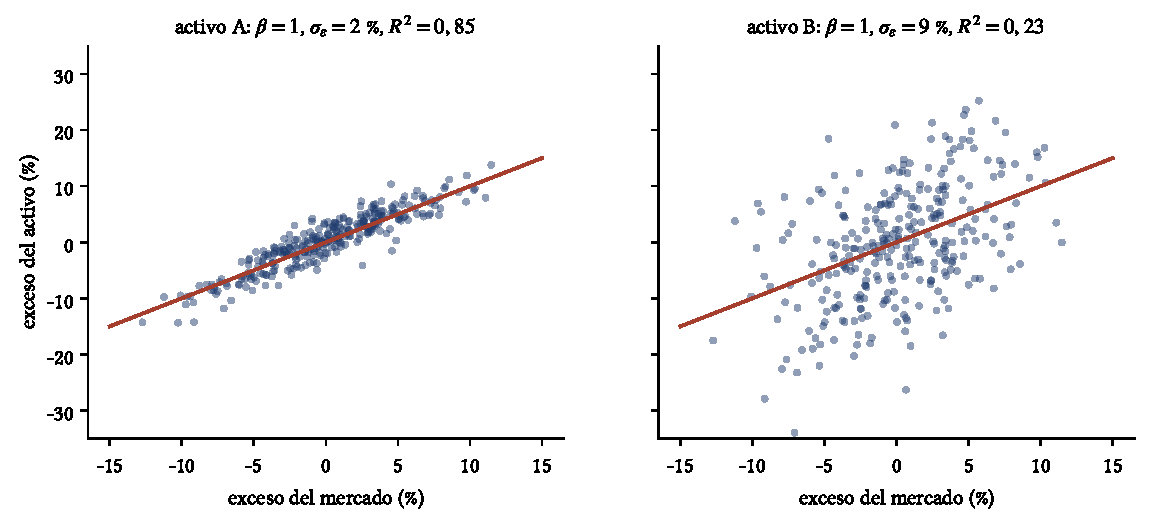
\includegraphics[width=\linewidth]{graficos/cap03_fig_riesgo.pdf}
\caption{Dos activos simulados con la misma beta ($\beta=1$, recta roja) y distinto riesgo idiosincrático.
En A los puntos se pegan a la recta: casi todo su riesgo es sistemático ($R^2$ alto). En B la nube es
mucho más ancha: la mayor parte de su riesgo es idiosincrático y desaparece en un portafolio diversificado.}
\label{fig:riesgo}
\end{figure}

% ---------------------------------------------------------------------
\section{Estimación por mínimos cuadrados ordinarios}
% ---------------------------------------------------------------------

Con una muestra $(x_t,y_t)$, $t=1,\dots,T$, donde $y_t=Z_{it}$ y $x_t=Z_{mt}$, escribimos
$\bar x,\bar y$ para las medias muestrales,
$S_{xx}=\sum_t(x_t-\bar x)^2$ y $S_{xy}=\sum_t(x_t-\bar x)(y_t-\bar y)$.

\begin{proposicion}[Estimadores MCO]\label{prop:mco}
Los valores $(\hat\alpha,\hat\beta)$ que minimizan la suma de residuos al cuadrado
$\mathrm{SRC}(a,b)=\sum_t(y_t-a-bx_t)^2$ son
\[
  \hat\beta=\frac{S_{xy}}{S_{xx}},\qquad \hat\alpha=\bar y-\hat\beta\,\bar x .
\]
\end{proposicion}

\begin{proof}
$\mathrm{SRC}$ es una función cuadrática convexa de $(a,b)$, así que su mínimo está donde se anulan las
derivadas parciales:
\begin{align}
  \frac{\partial\,\mathrm{SRC}}{\partial a} &= -2\sum_t(y_t-a-bx_t)=0, \tag{i}\\
  \frac{\partial\,\mathrm{SRC}}{\partial b} &= -2\sum_tx_t(y_t-a-bx_t)=0. \tag{ii}
\end{align}
De (i):
\begin{align*}
  \sum_ty_t-Ta-b\sum_tx_t &= 0\\
  T\bar y-Ta-bT\bar x &= 0\\
  a &= \bar y-b\,\bar x .
\end{align*}
Sustituyendo $a$ en (ii):
\begin{align*}
  \sum_tx_t\bigl(y_t-\bar y+b\bar x-bx_t\bigr) &= 0\\
  \sum_tx_t(y_t-\bar y)-b\sum_tx_t(x_t-\bar x) &= 0\\
  \sum_t(x_t-\bar x)(y_t-\bar y)-b\sum_t(x_t-\bar x)^2 &= 0\\
  S_{xy}-b\,S_{xx} &= 0\\
  b &= \frac{S_{xy}}{S_{xx}} .
\end{align*}
En la tercera línea restamos $\bar x$ dentro de cada suma, lo que no cambia nada porque
$\sum_t\bar x(y_t-\bar y)=0$ y $\sum_t\bar x(x_t-\bar x)=0$.
\end{proof}

La fórmula es la contraparte muestral de la Proposición~\ref{prop:betapob}: covarianza muestral entre
varianza muestral. La Figura~\ref{fig:mco} muestra qué significa ``minimizar la suma de residuos al
cuadrado'': de todas las rectas posibles, MCO elige la que hace más pequeña la suma de los cuadrados de
las distancias \emph{verticales} entre los puntos y la recta.

\begin{figure}[ht]
\centering
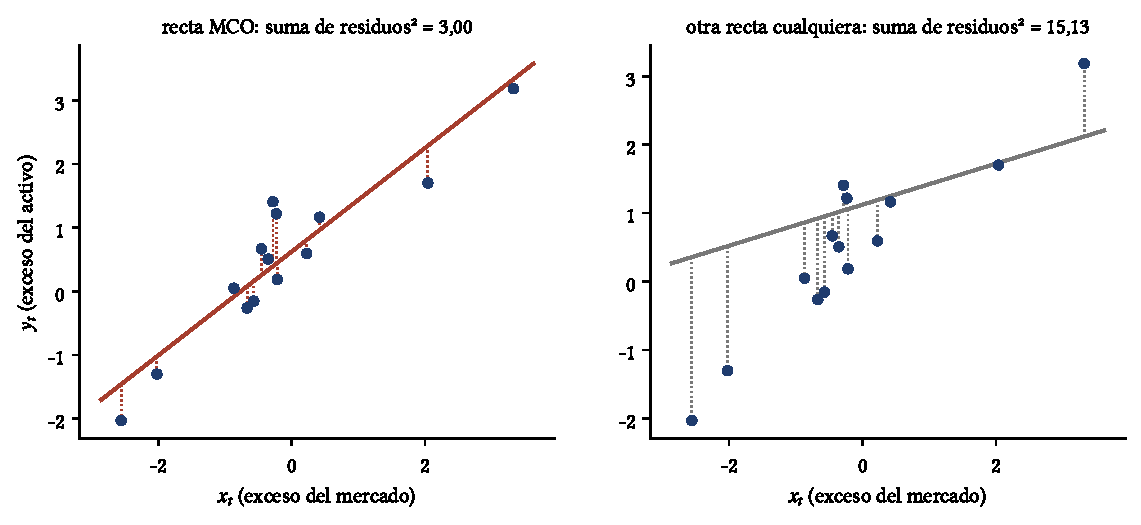
\includegraphics[width=\linewidth]{graficos/cap03_fig_mco.pdf}
\caption{Los residuos son las distancias verticales (líneas punteadas) entre cada observación y la recta.
La recta MCO (izquierda) tiene una suma de residuos al cuadrado de 3,00; cualquier otra recta, como la
de la derecha, tiene una suma mayor (aquí, 15,13). Datos simulados.}
\label{fig:mco}
\end{figure}

\begin{teorema}[Insesgamiento y varianza]\label{teo:varmco}
Suponga que $y_t=\alpha+\beta x_t+\varepsilon_t$ con $\E[\varepsilon_t\mid x_1,\dots,x_T]=0$,
$\Var(\varepsilon_t\mid x)=\sigma^2$ y $\Cov(\varepsilon_t,\varepsilon_s\mid x)=0$ para $t\ne s$. Entonces,
condicional en $x=(x_1,\dots,x_T)$,
\[
  \E[\hat\beta\mid x]=\beta,\qquad \Var(\hat\beta\mid x)=\frac{\sigma^2}{S_{xx}},\qquad
  \Var(\hat\alpha\mid x)=\sigma^2\Bigl(\frac1T+\frac{\bar x^2}{S_{xx}}\Bigr).
\]
\end{teorema}

\begin{proof}
Definimos los pesos $c_t=(x_t-\bar x)/S_{xx}$. Cumplen tres propiedades:
\begin{align*}
  \sum_tc_t    &= \frac{\sum_t(x_t-\bar x)}{S_{xx}} = 0,\\
  \sum_tc_tx_t &= \frac{\sum_t(x_t-\bar x)x_t}{S_{xx}} = \frac{\sum_t(x_t-\bar x)^2}{S_{xx}} = 1,\\
  \sum_tc_t^2  &= \frac{\sum_t(x_t-\bar x)^2}{S_{xx}^2} = \frac{1}{S_{xx}} .
\end{align*}
Como $\sum_t(x_t-\bar x)=0$, se cumple $S_{xy}=\sum_t(x_t-\bar x)y_t$, y entonces
\begin{align*}
  \hat\beta &= \sum_tc_ty_t\\
            &= \sum_tc_t\,(\alpha+\beta x_t+\varepsilon_t)\\
            &= \alpha\sum_tc_t+\beta\sum_tc_tx_t+\sum_tc_t\varepsilon_t\\
            &= \alpha\cdot0+\beta\cdot1+\sum_tc_t\varepsilon_t\\
            &= \beta+\sum_tc_t\varepsilon_t .
\end{align*}
Como los $c_t$ dependen solo de $x$:
\begin{align*}
  \E[\hat\beta\mid x] &= \beta+\sum_tc_t\,\E[\varepsilon_t\mid x]\\
                      &= \beta,\\
  \Var(\hat\beta\mid x) &= \sum_tc_t^2\,\Var(\varepsilon_t\mid x)\\
                        &= \sigma^2\sum_tc_t^2\\
                        &= \frac{\sigma^2}{S_{xx}} .
\end{align*}
Para $\hat\alpha$, con $\bar\varepsilon=\frac1T\sum_t\varepsilon_t$:
\begin{align*}
  \hat\alpha &= \bar y-\hat\beta\,\bar x\\
             &= (\alpha+\beta\bar x+\bar\varepsilon)-\hat\beta\,\bar x\\
             &= \alpha+\bar\varepsilon-(\hat\beta-\beta)\,\bar x .
\end{align*}
Los dos términos aleatorios no están correlacionados:
\begin{align*}
  \Cov(\bar\varepsilon,\hat\beta\mid x) &= \Cov\Bigl(\frac1T\sum_t\varepsilon_t,\ \sum_tc_t\varepsilon_t\Bigm|x\Bigr)\\
                                        &= \frac{\sigma^2}{T}\sum_tc_t\\
                                        &= 0 .
\end{align*}
Por tanto,
\begin{align*}
  \Var(\hat\alpha\mid x) &= \Var(\bar\varepsilon\mid x)+\bar x^2\,\Var(\hat\beta\mid x)\\
                         &= \frac{\sigma^2}{T}+\frac{\bar x^2\sigma^2}{S_{xx}}\\
                         &= \sigma^2\Bigl(\frac1T+\frac{\bar x^2}{S_{xx}}\Bigr). && \qedhere
\end{align*}
\end{proof}

\begin{teorema}[Gauss-Markov]\label{teo:gm}
Bajo los supuestos del Teorema~\ref{teo:varmco}, $\hat\beta$ tiene la menor varianza entre todos los
estimadores de $\beta$ que son lineales en $y$ e insesgados.
\end{teorema}

\begin{proof}
Sea $\tilde\beta=\sum_tk_ty_t$, con pesos $k_t$ que dependen solo de $x$. Su esperanza es
\begin{align*}
  \E[\tilde\beta\mid x] &= \sum_tk_t\,\E[y_t\mid x]\\
                        &= \sum_tk_t\,(\alpha+\beta x_t)\\
                        &= \alpha\sum_tk_t+\beta\sum_tk_tx_t .
\end{align*}
Para que sea igual a $\beta$ con cualquier $(\alpha,\beta)$ se necesita $\sum_tk_t=0$ y $\sum_tk_tx_t=1$. Su
varianza es $\Var(\tilde\beta\mid x)=\sigma^2\sum_tk_t^2$. Escribimos $k_t=c_t+d_t$, con los $c_t$ de MCO.
Como $k_t$ y $c_t$ cumplen las mismas dos restricciones:
\begin{align*}
  \sum_td_t    &= \sum_tk_t-\sum_tc_t = 0-0 = 0,\\
  \sum_td_tx_t &= \sum_tk_tx_t-\sum_tc_tx_t = 1-1 = 0,
\end{align*}
y entonces
\begin{align*}
  \sum_tc_td_t &= \frac{1}{S_{xx}}\sum_t(x_t-\bar x)\,d_t\\
               &= \frac{1}{S_{xx}}\Bigl(\sum_tx_td_t-\bar x\sum_td_t\Bigr)\\
               &= \frac{1}{S_{xx}}\,(0-0)\\
               &= 0 .
\end{align*}
Por tanto,
\begin{align*}
  \sum_tk_t^2 &= \sum_t(c_t+d_t)^2\\
              &= \sum_tc_t^2+2\sum_tc_td_t+\sum_td_t^2\\
              &= \frac{1}{S_{xx}}+0+\sum_td_t^2\\
              &\ge \frac{1}{S_{xx}},
\end{align*}
con igualdad solo si todos los $d_t$ son cero, es decir, si $\tilde\beta=\hat\beta$.
\end{proof}

\begin{proposicion}[Inferencia]\label{prop:inferencia}
Con $\hat\varepsilon_t=y_t-\hat\alpha-\hat\beta x_t$ y $s^2=\frac{1}{T-2}\sum_t\hat\varepsilon_t^2$, los
errores estándar son $\operatorname{ee}(\hat\beta)=\sqrt{s^2/S_{xx}}$ y
$\operatorname{ee}(\hat\alpha)=\sqrt{s^2(1/T+\bar x^2/S_{xx})}$. Si además los errores son normales,
$(\hat\beta-\beta)/\operatorname{ee}(\hat\beta)\sim t_{T-2}$ y lo mismo para $\hat\alpha$; sin
normalidad, el resultado vale asintóticamente con la normal estándar.
\end{proposicion}

Omitimos la demostración, que es estándar (véase Wooldridge, 2020, cap.~4). Lo importante para este
capítulo es su alcance: los errores estándar de la Proposición~\ref{prop:inferencia} suponen
homocedasticidad y ausencia de autocorrelación. El Capítulo~\ref{cap:hechos} mostró que los rendimientos
financieros tienen volatilidad cambiante; en el Capítulo~4 repetiremos las pruebas de este capítulo con
errores estándar robustos.

% ---------------------------------------------------------------------
\section{El CAPM}
% ---------------------------------------------------------------------

\subsection{La relación beta-rendimiento para un portafolio eficiente}

Considere $N$ activos riesgosos con vector de excesos de rendimiento esperados $\bm\mu$ (de dimensión
$N\times1$) y matriz de covarianzas $\bm\Sigma$, invertible, además de un activo libre de riesgo. Un
portafolio con pesos $\bm w$ en los activos riesgosos (y $1-\bm w'\bm1$ en el libre de riesgo) tiene
exceso esperado $\bm w'\bm\mu$ y varianza $\bm w'\bm\Sigma\bm w$. Un portafolio es \emph{eficiente} si
tiene la mínima varianza entre todos los que tienen su mismo exceso esperado.

\begin{teorema}[Relación beta-rendimiento]\label{teo:betarend}
Sea $q$ un portafolio eficiente con exceso esperado $\mu_q>0$. Entonces, para todo activo $i$,
\[
  \mu_i=\beta_{iq}\,\mu_q,\qquad \beta_{iq}=\frac{\Cov(Z_i,Z_q)}{\Var(Z_q)} .
\]
\end{teorema}

\begin{proof}
El portafolio eficiente resuelve $\min_{\bm w}\ \tfrac12\bm w'\bm\Sigma\bm w$ sujeto a
$\bm w'\bm\mu=\mu_q$. El lagrangiano y su condición de primer orden son
\begin{align*}
  \mathcal L &= \tfrac12\,\bm w'\bm\Sigma\bm w-\lambda\,(\bm w'\bm\mu-\mu_q),\\
  \frac{\partial\mathcal L}{\partial\bm w} &= \bm\Sigma\bm w-\lambda\bm\mu=\bm0,\\
  \bm\Sigma\bm w_q &= \lambda\,\bm\mu .
\end{align*}
Como $Z_q=\bm w_q'\bm Z$, la componente $i$ de $\bm\Sigma\bm w_q$ es la covarianza entre el activo $i$ y
el portafolio $q$:
\begin{equation}
  \Cov(Z_i,Z_q)=(\bm\Sigma\bm w_q)_i=\lambda\,\mu_i . \tag{a}
\end{equation}
Premultiplicando la condición de primer orden por $\bm w_q'$:
\begin{align*}
  \bm w_q'\bm\Sigma\bm w_q &= \lambda\,\bm w_q'\bm\mu\\
  \Var(Z_q)                &= \lambda\,\mu_q\\
  \lambda                  &= \frac{\Var(Z_q)}{\mu_q} .
\end{align*}
Sustituyendo $\lambda$ en (a):
\begin{align*}
  \mu_i &= \frac{\Cov(Z_i,Z_q)}{\lambda}\\
        &= \frac{\Cov(Z_i,Z_q)}{\Var(Z_q)}\,\mu_q\\
        &= \beta_{iq}\,\mu_q . && \qedhere
\end{align*}
\end{proof}

\begin{corolario}[Portafolio tangente]\label{cor:tangente}
De la demostración, todo portafolio eficiente tiene pesos proporcionales a $\bm\Sigma^{-1}\bm\mu$. El
portafolio eficiente formado solo por activos riesgosos (pesos que suman uno) es el \emph{portafolio
tangente}, $\bm w_q=\bm\Sigma^{-1}\bm\mu/(\bm1'\bm\Sigma^{-1}\bm\mu)$, y su razón de Sharpe es la máxima posible:
$\mu_q/\sigma_q=\sqrt{\bm\mu'\bm\Sigma^{-1}\bm\mu}$.
\end{corolario}

El Teorema~\ref{teo:betarend} es un resultado \emph{matemático}: vale para cualquier conjunto de activos y
cualquier portafolio eficiente, sin supuestos sobre el comportamiento de los inversionistas. El
\emph{contenido económico} del CAPM es la afirmación adicional de que, en equilibrio, si todos los
inversionistas optimizan en media-varianza con las mismas expectativas, el portafolio de mercado es el
portafolio tangente. Entonces $\mu_i=\beta_{im}\mu_m$ para todo activo: la \emph{recta del mercado de
valores} (SML, por sus siglas en inglés). La Figura~\ref{fig:capm} muestra la geometría: a la izquierda,
el portafolio tangente es el punto donde la recta que sale del activo libre de riesgo toca la frontera
eficiente; a la derecha, la SML y lo que significa una alfa distinta de cero.

\begin{figure}[ht]
\centering
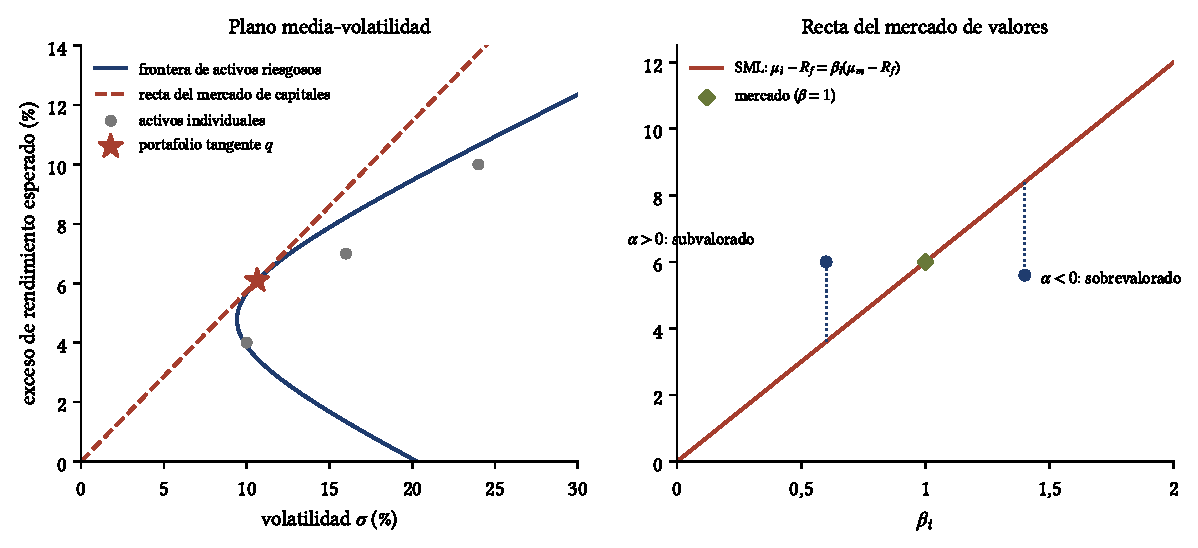
\includegraphics[width=\linewidth]{graficos/cap03_fig_capm.pdf}
\caption{Izquierda: la frontera de mínima varianza de tres activos riesgosos (parámetros ilustrativos) es
una hipérbola; la recta que parte del activo libre de riesgo y es tangente a ella (recta del mercado de
capitales) da la mejor relación entre riesgo y rendimiento, y toca la frontera en el portafolio tangente.
Derecha: la SML. Un activo por encima de ella ($\alpha>0$) rinde más de lo que su beta justifica; uno por
debajo ($\alpha<0$), menos.}
\label{fig:capm}
\end{figure}

\subsection{Cómo se contrasta}

En el modelo de mercado, tomando esperanzas, $\E[Z_{it}]=\alpha_i+\beta_i\E[Z_{mt}]$. Comparando con la
SML, \emph{el CAPM equivale a $\alpha_i=0$ para todo activo}. Esto da dos maneras de contrastarlo:
\begin{enumerate}[label=(\roman*),leftmargin=*]
  \item \textbf{En series de tiempo:} estimar el modelo de mercado para cada activo y probar
        $H_0:\alpha_i=0$ con el estadístico $t$. La prueba conjunta para todos los activos (Gibbons, Ross
        y Shanken, 1989) se estudia en el Capítulo~14.
  \item \textbf{En corte transversal:} estimar primero las betas y luego regresar los excesos de
        rendimiento promedio sobre ellas, $\bar Z_i=\gamma_0+\gamma_1\hat\beta_i+u_i$. El CAPM predice
        $\gamma_0=0$ y $\gamma_1=\bar Z_m$ (la prima de mercado).
\end{enumerate}

\begin{observacion}[La crítica de Roll]
Roll (1977) señaló que, por el Teorema~\ref{teo:betarend}, contrastar el CAPM es lo mismo que contrastar si
el portafolio usado como ``mercado'' es eficiente. Como el verdadero portafolio de mercado incluye todos los
activos de la economía (acciones, bonos, inmuebles, capital humano), y en la práctica se usa un índice
bursátil, un rechazo puede deberse a que el índice no es el mercado verdadero. Ilustraremos este punto en
el Ejercicio~\ref{ej:roll}.
\end{observacion}

% ---------------------------------------------------------------------
\section{Ejercicios resueltos}
% ---------------------------------------------------------------------

\begin{ejresuelto}{La beta del sector de servicios públicos, paso a paso}\label{ej:utils}
\enunciado Con los datos de Kenneth French (1949--2017), estime el modelo de mercado para el portafolio de
la industria de servicios públicos (\texttt{Utils}: electricidad, gas y agua). (a) Calcule $\hat\beta$ y
$\hat\alpha$ con las fórmulas de la Proposición~\ref{prop:mco} y sus errores estándar; (b) pruebe
$H_0:\beta=1$ y $H_0:\alpha=0$; (c) descomponga el riesgo; (d) compruebe con las funciones de regresión
de R y Python.

\solucion
\paso{Paso 1. Estimadores.} Con $T=819$ meses, las fórmulas de la Proposición~\ref{prop:mco} dan
\begin{align*}
  \hat\beta  &= \frac{S_{xy}}{S_{xx}}\\
             &= 0{,}5409,\\
  \hat\alpha &= \bar y-\hat\beta\,\bar x\\
             &= 0{,}0024625 \quad\text{(mensual)},\\
  12\,\hat\alpha &= 0{,}02955 \quad\text{(anual)},
\end{align*}
es decir, una alfa de $2{,}96$\,\% anual.

\paso{Paso 2. Pruebas.} Con $\operatorname{ee}(\hat\beta)=0{,}02497$ y $\operatorname{ee}(\hat\alpha)=0{,}00107$:
\begin{align*}
  t(\beta=1)  &= \frac{\hat\beta-1}{\operatorname{ee}(\hat\beta)}\\
              &= \frac{0{,}54087-1}{0{,}02497}\\
              &= \frac{-0{,}45913}{0{,}02497}\\
              &= -18{,}39,\\
  t(\alpha=0) &= \frac{\hat\alpha}{\operatorname{ee}(\hat\alpha)}\\
              &= \frac{0{,}0024625}{0{,}00107}\\
              &= 2{,}30 .
\end{align*}
La beta es claramente menor que 1. Un sector de servicios públicos, con demanda estable y tarifas
reguladas, es defensivo: cuando el mercado cae 10\,\%, el sector cae en promedio solo $5{,}4$\,\%. La alfa
tiene $p=0{,}022$: se rechaza $\alpha=0$ al 5\,\%. El sector rindió, en promedio, unos 3 puntos porcentuales
anuales más de lo que el CAPM predice para su beta.

\paso{Paso 3. Riesgo.} La varianza anual del exceso de rendimiento se divide así (Proposición~\ref{prop:descriesgo}):
\begin{align*}
  \underbrace{0{,}01730}_{\text{total}} &= \underbrace{0{,}00631}_{\text{sistemática}}+\underbrace{0{,}01099}_{\text{idiosincrática}},\\
  R^2 &= \frac{0{,}00631}{0{,}01730}\\
      &= 0{,}365 .
\end{align*}
En volatilidades (raíces cuadradas), el riesgo total es $13{,}15$\,\%, el sistemático $7{,}95$\,\% y el
idiosincrático $10{,}48$\,\%: las volatilidades no se suman, las varianzas sí. Solo un 36,5\,\% del riesgo
del sector es de mercado.

\codigoweb{cap03_ej01}
\salidaR{cap03_ej01_R.txt}
\lectura{cap03_ej01}

\RvsPy En R basta con \texttt{lm(y \textasciitilde{} x)}, que añade la constante automáticamente; en
\texttt{statsmodels} hay que añadirla de forma explícita con \texttt{sm.add\_constant}. Olvidarla es un
error muy común: produce una regresión por el origen que fuerza $\alpha=0$ y sesga la beta. Las fórmulas
manuales y las funciones dan los mismos valores en ambos lenguajes.

\begin{figure}[ht]
\centering
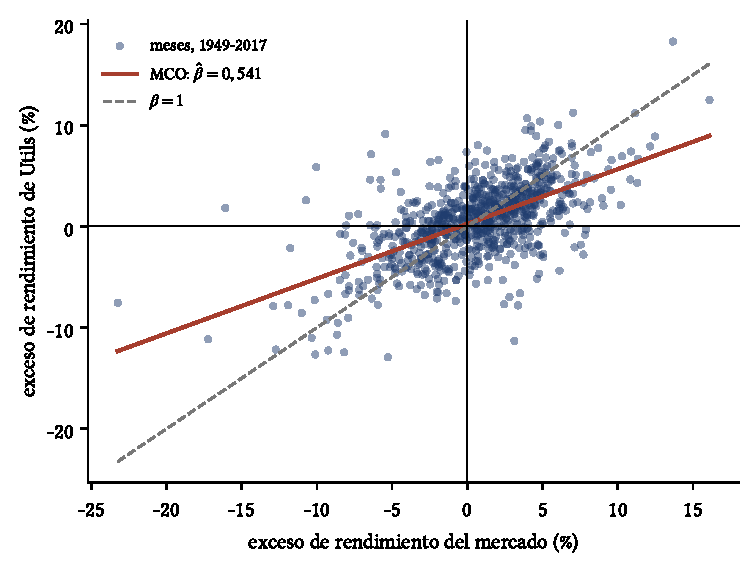
\includegraphics[width=0.66\linewidth]{graficos/cap03_fig_utils.pdf}
\caption{Excesos de rendimiento mensuales de \texttt{Utils} frente al mercado, 1949--2017. La recta MCO
(roja) es mucho más plana que la de $\beta=1$ (gris): el sector amplifica poco los movimientos del mercado.
La gran dispersión vertical alrededor de la recta es el riesgo idiosincrático.}
\label{fig:utils}
\end{figure}

\begin{conclusion}
El sector de servicios públicos tiene una beta de 0,54 y una alfa positiva y significativa de casi 3\,\%
anual. Si el CAPM fuera correcto, las empresas reguladas de este tipo tendrían un costo de capital bajo;
pero el sector rindió más de lo que su beta justifica, lo que anticipa la evidencia de la SML plana del
Ejercicio~\ref{ej:sml}.
\end{conclusion}
\end{ejresuelto}

\begin{ejresuelto}{El modelo de mercado en doce industrias}\label{ej:industrias}
\enunciado Estime el modelo de mercado para las 12 industrias. Reporte la alfa anual, su estadístico $t$,
la beta, el estadístico $t$ de $H_0:\beta=1$ y el $R^2$. ¿Cuántas alfas son significativas al 5\,\%?
¿Hay un patrón entre alfa y beta?

\solucion
\paso{Paso 1. Betas.} Van de 0,54 (\texttt{Utils}) a 1,25 (\texttt{BusEq}: equipos y tecnología). Todas
las betas son distintas de 1 al 5\,\% excepto la de \texttt{Shops} (comercio minorista, $t=-1{,}57$). Las
industrias defensivas (servicios públicos, telecomunicaciones, bienes no durables, energía, salud)
tienen betas menores que 1; las cíclicas (bienes durables, manufactura, tecnología), mayores.

\paso{Paso 2. Alfas.} Cuatro de doce alfas son significativas: \texttt{Utils} ($2{,}96$\,\%, $t=2{,}30$),
\texttt{NoDur} ($2{,}74$\,\%, $t=2{,}87$), \texttt{Hlth} ($3{,}32$\,\%, $t=2{,}49$) y \texttt{Other}
($-1{,}93$\,\%, $t=-2{,}24$). Si el CAPM fuera cierto y las pruebas fueran independientes, esperaríamos
$0{,}05\times12=0{,}6$ rechazos.

\paso{Paso 3. Patrón.} Ordenadas por beta, las alfas tienden a ser positivas en las industrias de beta baja
y negativas en las de beta alta. Las tres alfas positivas significativas corresponden a betas entre 0,54 y
0,87. Este patrón es el mismo que muestra la SML del Ejercicio~\ref{ej:sml}.

\codigoweb{cap03_ej02}
\salidaR{cap03_ej02_R.txt}
\lectura{cap03_ej02}

\RvsPy En R, \texttt{I(d[[i]] - d\$RF)} dentro de la fórmula hace que la resta se interprete como
aritmética y no como sintaxis de fórmulas; \texttt{sapply} recorre las industrias y devuelve una matriz.
En Python, el bucle construye un diccionario de diccionarios que \texttt{pandas} convierte en tabla.

\begin{figure}[ht]
\centering
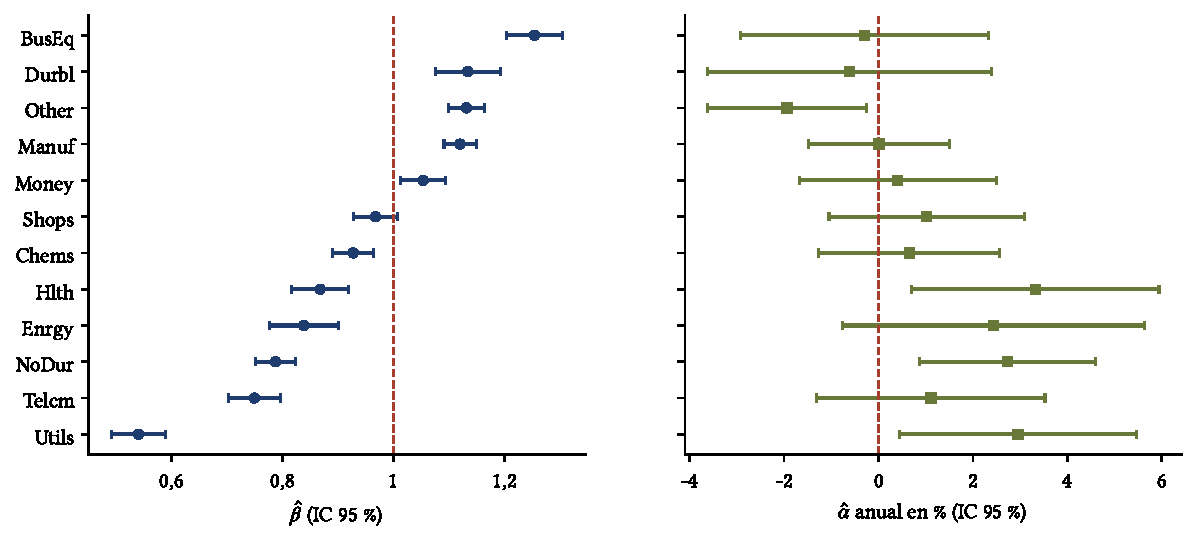
\includegraphics[width=\linewidth]{graficos/cap03_fig_betas.pdf}
\caption{Betas (izquierda) y alfas anuales (derecha) de las 12 industrias con intervalos de confianza al
95\,\%, ordenadas por beta. Las betas se estiman con mucha precisión; las alfas, con mucha menos: la mayoría
de sus intervalos incluyen el cero.}
\label{fig:betas}
\end{figure}

\begin{conclusion}
La beta resume bien la sensibilidad de cada industria al mercado y se estima con precisión. Las alfas, en
cambio, son imprecisas (intervalos de $\pm1{,}5$ a $\pm3{,}2$ puntos anuales) y, cuando son significativas,
siguen un patrón: positivas con beta baja y negativas con beta alta, en contra del CAPM.
\end{conclusion}
\end{ejresuelto}

\begin{ejresuelto}{La recta del mercado de valores es plana}\label{ej:sml}
\enunciado Con las betas del Ejercicio~\ref{ej:industrias} y los excesos de rendimiento promedio de cada
industria (anualizados), estime la regresión de corte transversal $\bar Z_i=\gamma_0+\gamma_1\hat\beta_i+u_i$
y compárela con la predicción del CAPM ($\gamma_0=0$, $\gamma_1=$ prima de mercado).

\solucion
\paso{Paso 1. Prima de mercado.} El exceso de rendimiento promedio del mercado es $7{,}74$\,\% anual; esa
es la pendiente que predice el CAPM.

\paso{Paso 2. Estimación.} $\hat\gamma_0=7{,}05$ ($t=4{,}89$) y $\hat\gamma_1=1{,}34$ ($t=0{,}90$), con
$R^2=0{,}075$. Comparada con la teórica, la pendiente estimada es
\begin{align*}
  \frac{\hat\gamma_1}{\bar Z_m} &= \frac{1{,}344}{7{,}744}\\
                                &= 0{,}17,
\end{align*}
menos de una quinta parte, y no es significativa; el intercepto, que debería ser cero, es grande y
significativo.

\paso{Paso 3. Interpretación.} En este período, una industria con beta 0,5 ganó en promedio casi lo
mismo que una con beta 1,25: la beta casi no explica las diferencias de rendimiento entre industrias. Es el
resultado clásico de Black, Jensen y Scholes (1972) y Fama y French (1992): la SML empírica es más plana
que la teórica.

\paso{Paso 4. Advertencias.} Con solo 12 observaciones la prueba de corte transversal tiene poca potencia.
Además, las betas son estimaciones con error: el error de medición en el regresor sesga $\hat\gamma_1$ hacia
cero (sesgo de atenuación). Con $\operatorname{ee}(\hat\beta)$ entre 0,015 y 0,032 y betas que varían de
0,54 a 1,25, el factor de atenuación estimado es de 0,99 (Ejercicio propuesto~3.4): el sesgo es mínimo y no
explica una pendiente tan plana.

\codigoweb{cap03_ej03}
\salidaR{cap03_ej03_R.txt}
\lectura{cap03_ej03}

\RvsPy En los dos lenguajes la regresión de corte transversal es una regresión ordinaria con 12
observaciones. En Python, \texttt{beta.rename("beta")} sirve solo para que el coeficiente aparezca con un
nombre legible en la tabla de resultados.

\begin{figure}[ht]
\centering
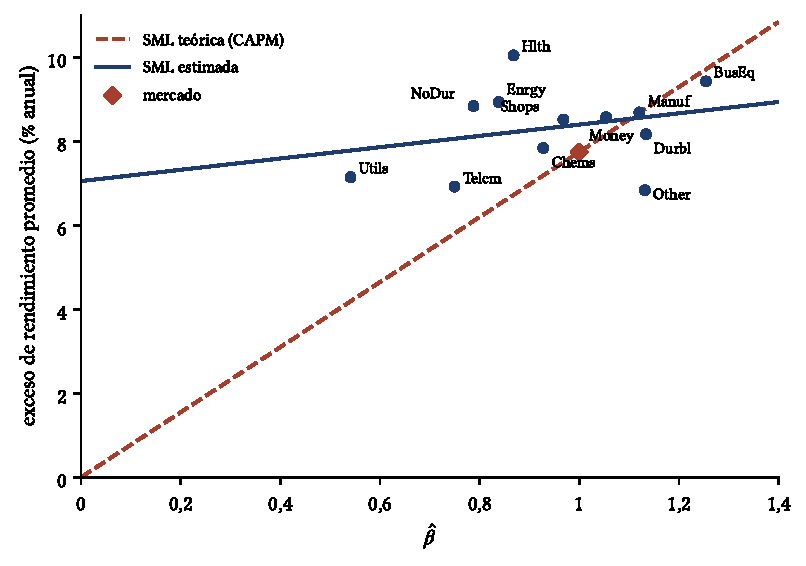
\includegraphics[width=0.74\linewidth]{graficos/cap03_fig_sml.pdf}
\caption{Recta del mercado de valores, 1949--2017. La línea discontinua es la predicción del CAPM: pasa
por el origen y por el mercado. La línea continua es la estimada con las 12 industrias: mucho más plana.
Las industrias de beta baja quedan por encima de la teórica (alfa positiva) y las de beta alta, por debajo.}
\label{fig:sml}
\end{figure}

\begin{conclusion}
Los datos no apoyan la predicción central del CAPM: los activos de beta alta no ganaron más que los de beta
baja en la proporción que el modelo predice. Esto no significa que la beta sea inútil (mide bien el riesgo
de mercado, Ejercicio~\ref{ej:industrias}), sino que no basta para explicar los rendimientos esperados. Los
modelos multifactoriales del Capítulo~14 nacen de esta evidencia.
\end{conclusion}
\end{ejresuelto}

\begin{ejresuelto}{¿Son estables las betas?}\label{ej:movil}
\enunciado Estime betas móviles con ventanas de 60 meses para \texttt{Utils}, \texttt{Enrgy} y
\texttt{BusEq}. Reporte su mínimo, máximo, último valor y desviación estándar, y discuta qué implica para
el uso de la beta en la práctica.

\solucion
\paso{Paso 1. Resultados.} La beta de \texttt{Utils} varió entre $-0{,}01$ (ventana que termina en marzo de
2001) y $0{,}81$ (agosto de 1974). La de \texttt{Enrgy}, entre $0{,}41$ (febrero de 1993) y $1{,}31$
(julio de 1982). La de \texttt{BusEq}, entre $1{,}00$ (noviembre de 2013) y $2{,}02$ (octubre de 2004).

\paso{Paso 2. Lectura económica.} La beta de tecnología se duplicó durante la burbuja de las empresas
puntocom: en la ventana 2000--2004 el mercado subía y bajaba al ritmo de las tecnológicas. En esos mismos
años la beta de servicios públicos llegó a cero: el sector se desacopló de un mercado dominado por la
tecnología. La beta de energía subió en la crisis petrolera de comienzos de los ochenta y en la caída de
precios de 2014--2016.

\paso{Paso 3. Magnitud.} La desviación estándar de las betas móviles (0,17 a 0,23) es de siete a nueve veces el
error estándar de las betas de muestra completa del Ejercicio~\ref{ej:industrias}: la incertidumbre que importa
en la práctica no es el error de estimación, sino el cambio de la beta en el tiempo.

\codigoweb{cap03_ej04}
\salidaR{cap03_ej04_R.txt}
\lectura{cap03_ej04}

\RvsPy En R se recorre cada ventana con \texttt{sapply}. En Python, \texttt{rolling(60).cov()} y
\texttt{rolling(60).var()} de \texttt{pandas} calculan todas las ventanas de una vez, de forma mucho más
rápida. Ambos usan el divisor $n-1$ en covarianza y varianza, que se cancela en el cociente.

\begin{figure}[ht]
\centering
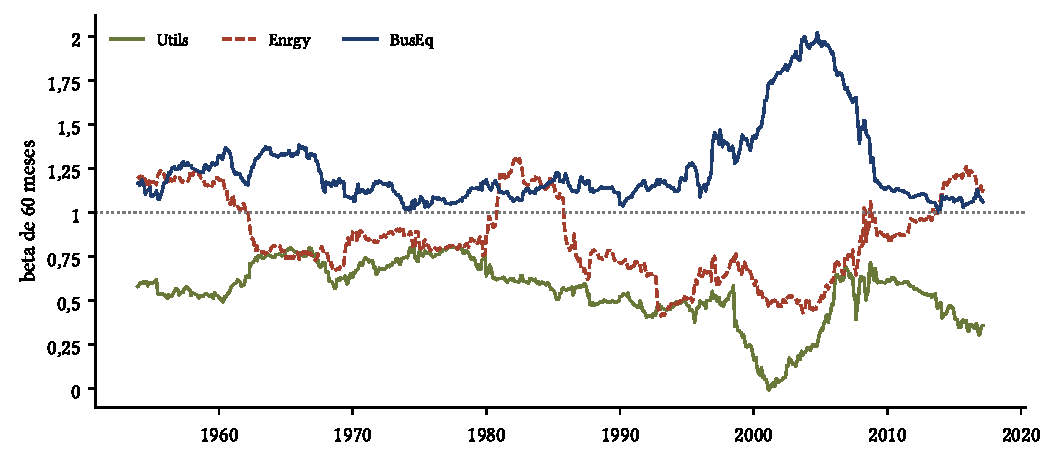
\includegraphics[width=0.92\linewidth]{graficos/cap03_fig_movil.pdf}
\caption{Betas móviles de 60 meses (cada punto usa los cinco años previos). Las betas cambian mucho: la de
tecnología (\texttt{BusEq}) llega a 2 en la burbuja puntocom, y la de servicios públicos (\texttt{Utils})
cae a cero en los mismos años.}
\label{fig:movil}
\end{figure}

\begin{conclusion}
Las betas no son constantes. Una beta estimada con cinco años de datos puede ser muy distinta de la que
regirá en los próximos cinco. En aplicaciones como el costo de capital conviene reportar la beta junto con
su evolución reciente y no como un número fijo.
\end{conclusion}
\end{ejresuelto}

\begin{ejresuelto}{El portafolio tangente y la crítica de Roll}\label{ej:roll}
\enunciado Con las 12 industrias: (a) calcule el portafolio tangente muestral (Corolario~\ref{cor:tangente})
y compare su razón de Sharpe con la del mercado; (b) verifique numéricamente el Teorema~\ref{teo:betarend}
con ese portafolio; (c) repita con el mercado y explique la diferencia.

\solucion
\paso{Paso 1. Pesos.} El portafolio tangente pone $64{,}9$\,\% en bienes no durables y vende en corto
$87{,}1$\,\% en ``otras'' industrias y $26{,}8$\,\% en químicos, entre otras posiciones. Su razón de
Sharpe anual es $0{,}809$, frente a $0{,}527$ del mercado.

\paso{Paso 2. Verificación del teorema.} Con las betas respecto del tangente, la máxima diferencia
$|\mu_i-\beta_{iq}\mu_q|$ es del orden de $10^{-18}$: cero con precisión de máquina. La SML se cumple
\emph{exactamente} en la muestra, como garantiza el Teorema~\ref{teo:betarend}.

\paso{Paso 3. Con el mercado.} Respecto del mercado, la alfa máxima es de $3{,}32$\,\% anual (salud). El
mercado no es el portafolio eficiente de estas 12 industrias en la muestra, y por eso aparecen alfas.

\paso{Paso 4. La lección de Roll.} La SML con el portafolio tangente no ``confirma'' nada: es una identidad
matemática. Y el portafolio tangente muestral no es un portafolio que alguien hubiera podido elegir en 1949,
porque usa medias y covarianzas que solo se conocen al final; sus posiciones cortas extremas son señal de que
optimiza el ruido de la muestra. Contrastar el CAPM es contrastar si el índice de mercado es eficiente, y la
respuesta depende de qué activos se incluyan.

\codigoweb{cap03_ej05}
\salidaR{cap03_ej05_R.txt}
\lectura{cap03_ej05}

\RvsPy Para obtener $\bm\Sigma^{-1}\bm\mu$ no conviene invertir la matriz: \texttt{solve(S, mu)} en R y
\texttt{np.linalg.solve(S, mu)} en Python resuelven el sistema lineal directamente, lo que es más rápido y
numéricamente más estable. La diferencia de $3{,}5\times10^{-18}$ (R) frente a $9{,}5\times10^{-18}$ (Python) en
el Paso~2 es solo error de redondeo de punto flotante.

\begin{figure}[ht]
\centering
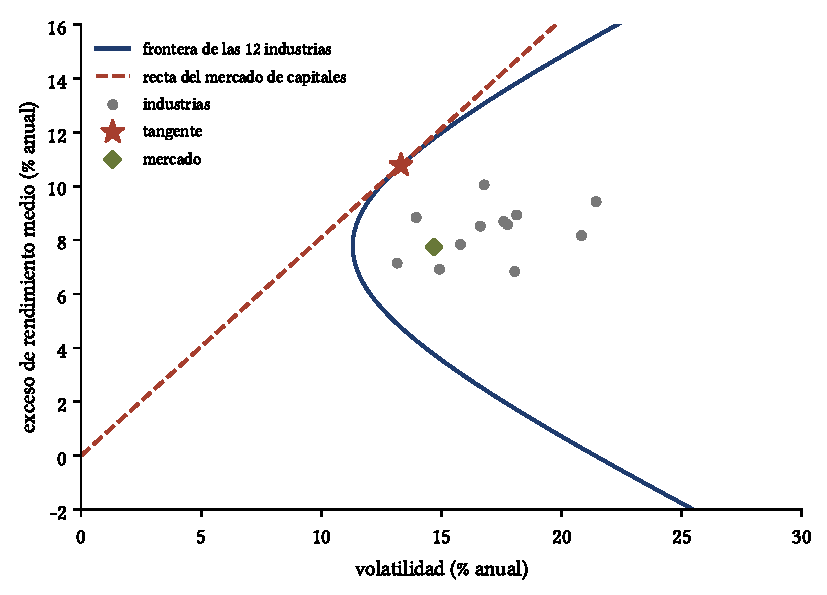
\includegraphics[width=0.74\linewidth]{graficos/cap03_fig_frontera.pdf}
\caption{Frontera de mínima varianza de las 12 industrias, 1949--2017, con la recta del mercado de capitales
que toca la frontera en el portafolio tangente (estrella). El mercado (rombo) queda dentro de la frontera:
no es eficiente con respecto a estas 12 industrias en la muestra.}
\label{fig:frontera}
\end{figure}

\begin{conclusion}
Respecto de un portafolio eficiente, la relación beta-rendimiento siempre se cumple; el CAPM tiene contenido
solo porque afirma que el mercado es ese portafolio. Con estos datos, el índice de mercado no es eficiente
respecto de las 12 industrias, lo que es otra forma de ver las alfas del Ejercicio~\ref{ej:industrias}.
\end{conclusion}
\end{ejresuelto}

% ---------------------------------------------------------------------
\section{Ejercicios propuestos}
% ---------------------------------------------------------------------

\begin{enumerate}[label=\textbf{\thechapter.\arabic*},leftmargin=*,itemsep=6pt]
  \item Demuestre que en la regresión MCO con constante se cumplen $\sum_t\hat\varepsilon_t=0$ y
  $\sum_tx_t\hat\varepsilon_t=0$, y que la recta pasa por el punto $(\bar x,\bar y)$. Use estas propiedades
  para demostrar que $\Var(y)=\hat\beta^2\Var(x)+\Var(\hat\varepsilon)$ en la muestra, como verificó el
  Ejercicio~\ref{ej:utils}.

  \item Demuestre que la beta de un portafolio es el promedio ponderado de las betas de los activos que lo
  forman, con los pesos del portafolio. ¿Qué beta tiene un portafolio con 50\,\% en \texttt{Utils} y
  50\,\% en \texttt{BusEq}? \textit{Respuesta: $0{,}5\times0{,}541+0{,}5\times1{,}254=0{,}898$.}

  \item Suponga que se regresa $Z_{it}$ sobre $Z_{mt}$ sin constante. Demuestre que la pendiente estimada es
  $\sum_tx_ty_t/\sum_tx_t^2$ y que difiere de $\hat\beta$ salvo que $\hat\alpha=0$ o $\bar x=0$.

  \item (Sesgo de atenuación.) Si $\hat\beta_i=\beta_i+v_i$ con $v_i$ independiente de $\beta_i$ y de varianza
  $\sigma^2_v$, demuestre que la pendiente de la regresión de $\bar Z_i$ sobre $\hat\beta_i$ converge a
  $\gamma_1\,\Var(\beta)/[\Var(\beta)+\sigma^2_v]$. Con los datos del Ejercicio~\ref{ej:industrias},
  estime el factor de atenuación. \textit{Pista: aproxime $\Var(\beta)$ por la varianza muestral de las
  betas menos el promedio de los $\operatorname{ee}^2$.}

  \item Demuestre la segunda parte del Corolario~\ref{cor:tangente}: la razón de Sharpe del portafolio
  tangente es $\sqrt{\bm\mu'\bm\Sigma^{-1}\bm\mu}$ y ningún otro portafolio tiene una razón mayor.
  \textit{Pista: use la desigualdad de Cauchy-Schwarz con el producto interno $\langle a,b\rangle=a'\bm\Sigma b$.}

  \item \emph{(Con datos.)} Divida la muestra en 1949--1982 y 1983--2017 y repita el
  Ejercicio~\ref{ej:sml} en cada mitad. ¿Es la SML plana en ambos períodos?

  \item \emph{(Con datos del Capítulo~\ref{cap:rendimientos}.)} Estime la beta de Credicorp, Southern Copper
  y Buenaventura respecto del índice S\&P/BVL Perú General, con rendimientos mensuales en soles y la tasa
  interbancaria del BCRP como tasa libre de riesgo. ¿Cuál es la acción más defensiva? ¿Cambian las betas
  si se usa el S\&P 500 como mercado?

  \item \emph{(Investigación.)} En la regulación tarifaria peruana, el costo de capital de las empresas de
  servicios públicos suele estimarse con un CAPM adaptado a mercados emergentes. Busque cómo lo calcula
  un organismo regulador peruano (por ejemplo, OSINERGMIN o SUNASS) y discuta qué beta usa y por qué.
\end{enumerate}

% ---------------------------------------------------------------------
\section{Resumen de fórmulas}
% ---------------------------------------------------------------------

\begin{table}[H]
\centering\small
\begin{tabular}{@{}ll@{}}
\toprule
Concepto & Fórmula \\
\midrule
Modelo de mercado & $Z_{it}=\alpha_i+\beta_iZ_{mt}+\varepsilon_{it}$ \\
Beta & $\beta_i=\Cov(Z_i,Z_m)/\Var(Z_m)$;\quad $\hat\beta=S_{xy}/S_{xx}$ \\
Alfa & $\hat\alpha=\bar y-\hat\beta\bar x$ \\
Riesgo total & $\Var(Z_i)=\beta_i^2\Var(Z_m)+\Var(\varepsilon_i)$;\quad $R^2=\rho^2(Z_i,Z_m)$ \\
Errores estándar & $\operatorname{ee}(\hat\beta)=\sqrt{s^2/S_{xx}}$;\quad $\operatorname{ee}(\hat\alpha)=\sqrt{s^2(1/T+\bar x^2/S_{xx})}$ \\
Relación beta-rendimiento & $\mu_i=\beta_{iq}\mu_q$ si $q$ es eficiente \\
Portafolio tangente & $\bm w_q=\bm\Sigma^{-1}\bm\mu/(\bm1'\bm\Sigma^{-1}\bm\mu)$;\quad $SR_q=\sqrt{\bm\mu'\bm\Sigma^{-1}\bm\mu}$ \\
SML de corte transversal & $\bar Z_i=\gamma_0+\gamma_1\hat\beta_i+u_i$;\quad CAPM: $\gamma_0=0$, $\gamma_1=\bar Z_m$ \\
\bottomrule
\end{tabular}
\caption{Fórmulas principales del Capítulo 3.}
\end{table}

\section*{Referencias}
\begin{itemize}[leftmargin=*]
  \item Black, F., Jensen, M. C. y Scholes, M. (1972). The capital asset pricing model: some empirical
        tests. En M. C. Jensen (ed.), \emph{Studies in the Theory of Capital Markets}. Praeger.
  \item Fama, E. F. y French, K. R. (1992). The cross-section of expected stock returns. \emph{The Journal
        of Finance}, 47(2), 427--465.
  \item French, K. R. \emph{Data Library}. Tuck School of Business, Dartmouth College.
        \url{https://mba.tuck.dartmouth.edu/pages/faculty/ken.french/data_library.html}.
  \item Gibbons, M. R., Ross, S. A. y Shanken, J. (1989). A test of the efficiency of a given portfolio.
        \emph{Econometrica}, 57(5), 1121--1152.
  \item Lintner, J. (1965). The valuation of risk assets and the selection of risky investments in stock
        portfolios and capital budgets. \emph{The Review of Economics and Statistics}, 47(1), 13--37.
  \item Roll, R. (1977). A critique of the asset pricing theory's tests. Part I: On past and potential
        testability of the theory. \emph{Journal of Financial Economics}, 4(2), 129--176.
  \item Sharpe, W. F. (1964). Capital asset prices: a theory of market equilibrium under conditions of
        risk. \emph{The Journal of Finance}, 19(3), 425--442.
  \item Wooldridge, J. M. (2020). \emph{Introductory Econometrics: A Modern Approach} (7.ª ed.). Cengage.
\end{itemize}

% =====================================================================
%  Capítulo 4. Problemas del MCO con datos financieros
% =====================================================================
\chapter[Problemas del MCO con datos financieros]{Problemas del MCO con datos financieros: heterocedasticidad, autocorrelación y cambios estructurales}\label{cap:robustos}

\section*{Objetivos de aprendizaje}
Al terminar este capítulo, el lector podrá:
\begin{enumerate}[label=\arabic*.,leftmargin=*]
  \item Explicar por qué la heterocedasticidad y la autocorrelación no sesgan los estimadores MCO pero
        invalidan sus errores estándar clásicos, y cuantificar el error.
  \item Derivar y calcular los errores estándar robustos de White (HC0, HC1) y de Newey-West (HAC).
  \item Aplicar las pruebas de Breusch-Pagan y de White, y una prueba de autocorrelación robusta a la
        heterocedasticidad.
  \item Reconocer el problema de las regresiones con horizontes traslapados y corregir su inferencia.
  \item Contrastar cambios estructurales con fecha conocida (Chow), con fecha desconocida (sup-F) y de
        forma secuencial (CUSUM).
\end{enumerate}

\section*{Motivación}
Los Capítulos~\ref{cap:hechos} y~\ref{cap:capm} dejaron dos cuentas pendientes. En el primero, la prueba de
Ljung-Box rechazó que los rendimientos del Brent no estuvieran autocorrelacionados ($p=0{,}004$), y
advertimos que la prueba podía estar engañada por la volatilidad cambiante. En el segundo, calculamos
estadísticos $t$ para las alfas y betas del CAPM con fórmulas que suponen varianza constante y errores no
correlacionados, dos supuestos que los datos financieros violan sistemáticamente.

El problema es general. MCO sigue siendo un buen estimador con datos financieros, pero sus errores estándar
clásicos pueden estar muy equivocados, y con ellos todas las pruebas de hipótesis y los intervalos de
confianza. Este capítulo muestra cuánto se equivocan, cómo corregirlos y qué ocurre con las conclusiones de
los capítulos anteriores cuando se corrigen. Cierra con otro problema típico de las series financieras
largas: que los parámetros cambien en el tiempo.

\paragraph{Datos del capítulo.} Reutilizamos la base de Kenneth French (1949--2017), el Brent diario
(1987--2026) y el S\&P 500 mensual de Shiller con dividendos (1871--2023). Las simulaciones de Monte Carlo
de la teoría están en \texttt{codigo/Python/cap04\_figuras\_teoria.py}, con semilla fija.

% ---------------------------------------------------------------------
\section{Heterocedasticidad}
% ---------------------------------------------------------------------

\begin{definicion}[Heterocedasticidad]
En el modelo $y_t=\alpha+\beta x_t+\varepsilon_t$ con $\E[\varepsilon_t\mid x]=0$, hay
\emph{heterocedasticidad} si la varianza condicional $\sigma^2_t=\Var(\varepsilon_t\mid x)$ cambia entre
observaciones.
\end{definicion}

En el modelo de mercado hay una razón económica para esperarla: en los meses de grandes movimientos del
mercado (crisis, pánicos, burbujas) también son grandes los movimientos idiosincráticos de cada industria.
La varianza del residuo crece entonces con $|x_t|$, y la nube de puntos tiene forma de embudo
(Figura~\ref{fig:hetero}, izquierda).

\begin{proposicion}[MCO con heterocedasticidad]\label{prop:mcohetero}
Si los errores no están correlacionados pero $\Var(\varepsilon_t\mid x)=\sigma_t^2$, entonces $\hat\beta$
sigue siendo insesgado, pero
\[
  \Var(\hat\beta\mid x)=\frac{\sum_t(x_t-\bar x)^2\sigma_t^2}{S_{xx}^2},
\]
que en general es distinta de la fórmula clásica $\sigma^2/S_{xx}$. En muestras grandes, el cociente entre
la varianza verdadera y la que estima la fórmula clásica tiende a
\[
  \frac{\E\bigl[(x_t-\mu_x)^2\sigma_t^2\bigr]}{\Var(x_t)\,\E[\sigma_t^2]},
\]
que es mayor que 1 cuando la varianza del error es mayor en las observaciones con $x_t$ alejado de su media.
\end{proposicion}

\begin{proof}
La demostración del Teorema~\ref{teo:varmco} mostró, sin usar ningún supuesto sobre la varianza, que
\begin{align*}
  \hat\beta &= \beta+\sum_tc_t\varepsilon_t, \qquad c_t=\frac{x_t-\bar x}{S_{xx}},
\end{align*}
de modo que $\E[\hat\beta\mid x]=\beta$: el insesgamiento se mantiene. Como los errores no están
correlacionados:
\begin{align*}
  \Var(\hat\beta\mid x) &= \sum_tc_t^2\,\sigma_t^2\\
                        &= \frac{\sum_t(x_t-\bar x)^2\,\sigma_t^2}{S_{xx}^2} .
\end{align*}
La fórmula clásica estima $s^2/S_{xx}$, y $s^2$ converge al promedio de las varianzas, $\E[\sigma_t^2]$. El
cociente entre ambas, dividiendo numerador y denominador entre $T$, es
\begin{align*}
  \frac{\Var(\hat\beta\mid x)}{s^2/S_{xx}}
    &= \frac{\sum_t(x_t-\bar x)^2\,\sigma_t^2}{S_{xx}^2}\cdot\frac{S_{xx}}{s^2}\\
    &= \frac{\frac1T\sum_t(x_t-\bar x)^2\,\sigma_t^2}{\frac1TS_{xx}\cdot s^2}\\
    &\longrightarrow \frac{\E\bigl[(x_t-\mu_x)^2\sigma_t^2\bigr]}{\Var(x_t)\,\E[\sigma_t^2]} .
\end{align*}
Por último, el numerador se descompone así:
\begin{align*}
  \E\bigl[(x_t-\mu_x)^2\sigma_t^2\bigr] &= \E\bigl[(x_t-\mu_x)^2\bigr]\,\E[\sigma_t^2]+\Cov\bigl((x_t-\mu_x)^2,\sigma_t^2\bigr)\\
                                        &= \Var(x_t)\,\E[\sigma_t^2]+\Cov\bigl((x_t-\mu_x)^2,\sigma_t^2\bigr),
\end{align*}
y el cociente es mayor que 1 si y solo si esa covarianza es positiva.
\end{proof}

\subsection{El estimador de White}

En notación matricial, con $\bm X$ la matriz $T\times k$ de regresores (incluida la columna de unos),
$\hat{\bm\beta}=(\bm X'\bm X)^{-1}\bm X'\bm y$ y $\hat{\bm\beta}-\bm\beta=(\bm X'\bm X)^{-1}\bm X'\bm\varepsilon$.
Si los errores no están correlacionados,
\[
  \Var(\hat{\bm\beta}\mid\bm X)=(\bm X'\bm X)^{-1}\Bigl(\sum_t\sigma_t^2\,\bm x_t\bm x_t'\Bigr)(\bm X'\bm X)^{-1},
\]
donde $\bm x_t'$ es la fila $t$ de $\bm X$. Por su forma, se le llama matriz \emph{sándwich}: el ``pan'' es
$(\bm X'\bm X)^{-1}$ y el ``relleno'' es la suma central. White (1980) mostró que no hace falta conocer cada
$\sigma_t^2$: basta con reemplazarla por el residuo al cuadrado.

\begin{teorema}[White, 1980]\label{teo:white}
Bajo condiciones de regularidad (observaciones independientes o débilmente dependientes y momentos
finitos de orden cuatro), el estimador
\[
  \widehat{\bm V}_{\mathrm{HC0}}=(\bm X'\bm X)^{-1}\Bigl(\sum_t\hat\varepsilon_t^2\,\bm x_t\bm x_t'\Bigr)(\bm X'\bm X)^{-1}
\]
es consistente para la varianza de $\hat{\bm\beta}$, en el sentido de que
$T\widehat{\bm V}_{\mathrm{HC0}}$ converge a la varianza asintótica de $\sqrt T(\hat{\bm\beta}-\bm\beta)$, haya
o no heterocedasticidad.
\end{teorema}

La idea de la demostración es que cada $\hat\varepsilon_t^2$ es un estimador muy malo de $\sigma_t^2$, pero
el promedio $\frac1T\sum_t\hat\varepsilon_t^2\bm x_t\bm x_t'$ converge al promedio de
$\sigma_t^2\bm x_t\bm x_t'$ por la ley de los grandes números, que es lo único que se necesita. En muestras
finitas se suele usar la corrección por grados de libertad
$\widehat{\bm V}_{\mathrm{HC1}}=\frac{T}{T-k}\widehat{\bm V}_{\mathrm{HC0}}$.

La Figura~\ref{fig:hetero} (derecha) muestra con una simulación la magnitud del problema. Con errores cuya
desviación estándar crece con $|x_t|$, la prueba $t$ clásica de una hipótesis cierta la rechaza alrededor del
23\,\% de las veces, aunque se haga al 5\,\%, y el problema no mejora con más datos, porque el error de la
fórmula clásica no desaparece con $T$. La prueba con errores HC1 se acerca al 5\,\% a medida que crece la
muestra: 9,6\,\% con $T=50$ y 4,8\,\% con $T=1\,000$.

\begin{figure}[ht]
\centering
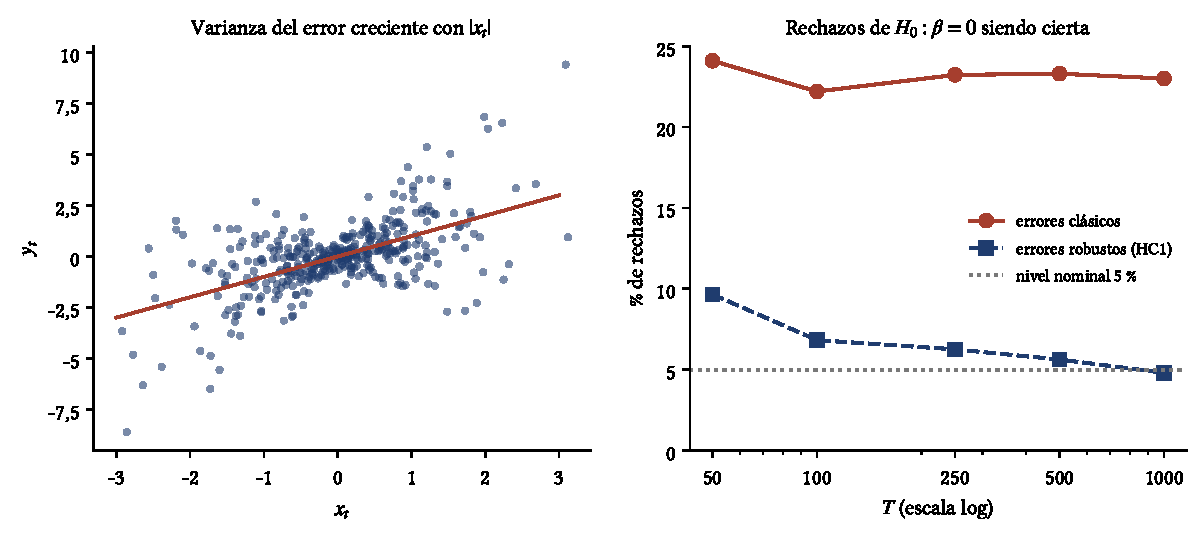
\includegraphics[width=\linewidth]{graficos/cap04_fig_hetero.pdf}
\caption{Izquierda: datos simulados con $\beta=1$ cuya varianza del error crece con $|x_t|$: la nube tiene
forma de embudo, más ancha en los extremos. Derecha: porcentaje de rechazos de una hipótesis cierta con la
prueba $t$ al 5\,\%, en 4\,000 simulaciones por tamaño de muestra. Con errores clásicos se rechaza en torno
al 23\,\% de las veces sin importar $T$; con errores robustos, el porcentaje se acerca al 5\,\%.}
\label{fig:hetero}
\end{figure}

\subsection{Pruebas de heterocedasticidad}

\begin{definicion}[Pruebas de Breusch-Pagan y de White]
Se estima la regresión auxiliar de $\hat\varepsilon_t^2$ sobre una constante y un conjunto de $q$ variables
$\bm z_t$, y se calcula $LM=T\cdot R^2_{\mathrm{aux}}$. Bajo homocedasticidad, $LM$ converge a una
$\chi^2_q$. En la prueba de \emph{Breusch-Pagan} (en la versión de Koenker), $\bm z_t$ son los regresores
originales; en la de \emph{White}, son los regresores, sus cuadrados y sus productos cruzados.
\end{definicion}

\begin{observacion}
La diferencia importa en el modelo de mercado. Si la varianza del residuo crece con $|x_t|$ (tanto en las
subidas como en las caídas del mercado), su relación con $x_t$ es simétrica y no lineal: la regresión
auxiliar sobre $x_t$ no la detecta, pero la regresión sobre $x_t$ y $x_t^2$ sí.
\end{observacion}

% ---------------------------------------------------------------------
\section{Autocorrelación y errores de Newey-West}
% ---------------------------------------------------------------------

\subsection{La varianza de largo plazo}

Escribimos $\sqrt T(\hat{\bm\beta}-\bm\beta)=\bigl(\tfrac1T\bm X'\bm X\bigr)^{-1}\tfrac{1}{\sqrt T}\sum_t\bm u_t$,
con $\bm u_t=\bm x_t\varepsilon_t$. Toda la incertidumbre de $\hat{\bm\beta}$ proviene de la suma
$\sum_t\bm u_t$. Si los $\bm u_t$ están autocorrelacionados, su varianza no es la suma de varianzas: es la
misma situación que la agregación temporal de rendimientos (Proposición~\ref{prop:agregmom}).

\begin{proposicion}[Varianza de largo plazo]\label{prop:vlp}
Si $\bm u_t$ es estacionario con media cero y autocovarianzas $\bm\Gamma_j=\E[\bm u_t\bm u_{t-j}']$, entonces
\[
  \Var\Bigl(\frac1{\sqrt T}\sum_{t=1}^T\bm u_t\Bigr)=\bm\Gamma_0+\sum_{j=1}^{T-1}\Bigl(1-\frac jT\Bigr)
  \bigl(\bm\Gamma_j+\bm\Gamma_j'\bigr)\ \longrightarrow\ \bm S=\bm\Gamma_0+\sum_{j=1}^{\infty}\bigl(\bm\Gamma_j+\bm\Gamma_j'\bigr).
\]
\end{proposicion}

\begin{proof}
La varianza de la suma es la suma de todas las covarianzas. Agrupamos los pares $(t,s)$ por su distancia:
hay $T$ pares con $t=s$; para cada $j\ge1$ hay $T-j$ pares con $t-s=j$, que aportan $\bm\Gamma_j$, y $T-j$
con $s-t=j$, que aportan $\bm\Gamma_j'$:
\begin{align*}
  \Var\Bigl(\frac1{\sqrt T}\sum_{t=1}^T\bm u_t\Bigr)
    &= \frac1T\sum_{t=1}^T\sum_{s=1}^T\E[\bm u_t\bm u_s']\\
    &= \frac1T\Bigl[T\,\bm\Gamma_0+\sum_{j=1}^{T-1}(T-j)\,\bm\Gamma_j+\sum_{j=1}^{T-1}(T-j)\,\bm\Gamma_j'\Bigr]\\
    &= \bm\Gamma_0+\sum_{j=1}^{T-1}\Bigl(1-\frac jT\Bigr)\bigl(\bm\Gamma_j+\bm\Gamma_j'\bigr).
\end{align*}
Si las autocovarianzas son sumables, el último término converge a $\sum_{j\ge1}(\bm\Gamma_j+\bm\Gamma_j')$
cuando $T\to\infty$.
\end{proof}

La matriz $\bm S$ se llama \emph{varianza de largo plazo}. Con errores no autocorrelacionados se reduce a
$\bm\Gamma_0$, que es lo que estima el relleno de White.

\begin{definicion}[Estimador de Newey-West]
Con $\hat{\bm u}_t=\bm x_t\hat\varepsilon_t$ y $\hat{\bm\Gamma}_j=\sum_{t=j+1}^T\hat{\bm u}_t\hat{\bm u}_{t-j}'$,
\[
  \widehat{\bm V}_{\mathrm{NW}}=(\bm X'\bm X)^{-1}\Bigl[\hat{\bm\Gamma}_0+\sum_{j=1}^{L}\Bigl(1-\frac{j}{L+1}\Bigr)
  \bigl(\hat{\bm\Gamma}_j+\hat{\bm\Gamma}_j'\bigr)\Bigr](\bm X'\bm X)^{-1}.
\]
\end{definicion}

Los pesos $1-j/(L+1)$ (núcleo de Bartlett) decrecen linealmente hasta cero. Newey y West (1987) mostraron que
con ellos la matriz estimada es siempre semidefinida positiva (una varianza nunca negativa), lo que no
ocurriría con pesos iguales a 1, y que el estimador es consistente si $L$ crece con $T$, pero más despacio.
Una regla práctica habitual es $L=\lfloor4(T/100)^{2/9}\rfloor$ (Newey y West, 1994), que da $L=6$ con
$T=819$ meses. Con $L=0$ el estimador se reduce a HC0, por lo que Newey-West es robusto a la vez a la
heterocedasticidad y a la autocorrelación (HAC, por sus siglas en inglés).

\subsection{Una prueba de autocorrelación robusta}

Volvemos a la deuda del Capítulo~\ref{cap:hechos}.

\begin{proposicion}[Autocorrelación muestral bajo heterocedasticidad condicional]\label{prop:acfrob}
Si $r_t$ es estacionario, con media cero, cuarto momento finito y $\E[r_t\mid\mathcal F_{t-1}]=0$ (como el
proceso de la Proposición~\ref{prop:mds}), entonces, para cada $j\ge1$,
\[
  \sqrt T\,\hat\rho_j\xrightarrow{d}N\Bigl(0,\ \frac{\E[r_t^2r_{t-j}^2]}{\sigma^4}\Bigr).
\]
\end{proposicion}

\begin{proof}[Esbozo de demostración]
Como la media es cero, en muestras grandes
\begin{align*}
  \sqrt T\,\hat\rho_j &\approx \frac{\frac{1}{\sqrt T}\sum_tr_t\,r_{t-j}}{\frac1T\sum_tr_t^2},\\
  \frac1T\sum_tr_t^2  &\xrightarrow{p}\sigma^2 .
\end{align*}
En el numerador, $v_t=r_t\,r_{t-j}$ es una diferencia de martingala:
\begin{align*}
  \E[v_t\mid\mathcal F_{t-1}] &= \E[r_t\,r_{t-j}\mid\mathcal F_{t-1}]\\
                              &= r_{t-j}\,\E[r_t\mid\mathcal F_{t-1}]\\
                              &= 0 .
\end{align*}
Por tanto no está autocorrelacionada, y el teorema central del límite para diferencias de martingala da
\begin{align*}
  \frac1{\sqrt T}\sum_tv_t &\xrightarrow{d}N\bigl(0,\ \E[v_t^2]\bigr) = N\bigl(0,\ \E[r_t^2r_{t-j}^2]\bigr).
\end{align*}
Por el teorema de Slutsky,
\begin{align*}
  \sqrt T\,\hat\rho_j &\xrightarrow{d} N\Bigl(0,\ \frac{\E[r_t^2r_{t-j}^2]}{\sigma^4}\Bigr). && \qedhere
\end{align*}
\end{proof}

Si los $r_t$ son i.i.d., $\E[r_t^2r_{t-j}^2]=\sigma^4$ y se recupera la banda de Bartlett. Con agrupamiento de
volatilidad, $\E[r_t^2r_{t-j}^2]=\sigma^4+\Cov(r_t^2,r_{t-j}^2)>\sigma^4$ y la varianza verdadera es mayor. La
versión muestral da una banda robusta, $\pm1{,}96\sqrt{\hat v_j}$ con
$\hat v_j=\sum_tr_t^2r_{t-j}^2/(\sum_tr_t^2)^2$, y una prueba conjunta $Q^*(m)=\sum_{j=1}^m\hat\rho_j^2/\hat v_j$,
que se compara con una $\chi^2_m$. Esta es una versión simple, que ignora las covarianzas entre los $\hat\rho_j$
de distintos rezagos; Lobato, Nankervis y Savin (2001) desarrollan versiones más generales.

\subsection{Regresiones con horizontes traslapados}

En finanzas es frecuente preguntar si una variable predice el rendimiento de los próximos $k$ períodos y
usar, para ganar observaciones, rendimientos de $k$ meses que se calculan cada mes. Los datos se
\emph{traslapan}: el rendimiento de enero a diciembre y el de febrero a enero comparten once meses.

\begin{proposicion}[Correlación inducida por el traslape]\label{prop:traslape}
Si los rendimientos de un período $g_t$ son no correlacionados con varianza $\sigma^2$ y
$y_t=\sum_{i=1}^kg_{t+i}$, entonces $\operatorname{Corr}(y_t,y_{t-j})=(k-j)/k$ para $0\le j<k$, y cero para
$j\ge k$.
\end{proposicion}

\begin{proof}
Escribimos ambas sumas:
\begin{align*}
  y_t     &= g_{t+1}+g_{t+2}+\cdots+g_{t+k},\\
  y_{t-j} &= g_{t-j+1}+g_{t-j+2}+\cdots+g_{t-j+k}.
\end{align*}
Para $0\le j<k$ comparten exactamente los $k-j$ rendimientos $g_{t+1},\dots,g_{t-j+k}$. Como los $g$ no
están correlacionados, solo esos términos comunes aportan covarianza:
\begin{align*}
  \Cov(y_t,y_{t-j})            &= \sum_{i=t+1}^{t-j+k}\Var(g_i)\\
                               &= (k-j)\,\sigma^2,\\
  \Var(y_t)                    &= k\,\sigma^2,\\
  \operatorname{Corr}(y_t,y_{t-j}) &= \frac{(k-j)\,\sigma^2}{k\,\sigma^2}\\
                               &= \frac{k-j}{k}.
\end{align*}
Para $j\ge k$ no hay términos comunes y la covarianza es cero.
\end{proof}

\begin{proposicion}[Factor de inflación con un predictor persistente]\label{prop:inflacion}
Suponga que el predictor $x_t$, centrado, es estacionario e independiente del error $\varepsilon_t$, con
autocorrelaciones $\rho_x(j)$ y $\rho_\varepsilon(j)$. Entonces, en muestras grandes, el cociente entre la
varianza verdadera de $\hat\beta$ y la que estima la fórmula clásica es
\[
  1+2\sum_{j=1}^{\infty}\rho_x(j)\,\rho_\varepsilon(j).
\]
\end{proposicion}

\begin{proof}
La incertidumbre de $\hat\beta$ proviene de $\sum_tu_t$ con $u_t=x_t\varepsilon_t$. Por independencia entre
$x$ y $\varepsilon$:
\begin{align*}
  \E[u_t\,u_{t-j}] &= \E[x_t\,x_{t-j}\,\varepsilon_t\,\varepsilon_{t-j}]\\
                   &= \E[x_t\,x_{t-j}]\,\E[\varepsilon_t\,\varepsilon_{t-j}]\\
                   &= \gamma_x(j)\,\gamma_\varepsilon(j)\\
                   &= \gamma_x(0)\,\gamma_\varepsilon(0)\,\rho_x(j)\,\rho_\varepsilon(j).
\end{align*}
Por la Proposición~\ref{prop:vlp}, la varianza de largo plazo es
\begin{align*}
  S &= \E[u_t^2]+2\sum_{j\ge1}\E[u_t\,u_{t-j}]\\
    &= \gamma_x(0)\,\gamma_\varepsilon(0)\Bigl[1+2\sum_{j\ge1}\rho_x(j)\,\rho_\varepsilon(j)\Bigr].
\end{align*}
La fórmula clásica usa solo $\E[u_t^2]=\gamma_x(0)\gamma_\varepsilon(0)$, así que el cociente es
\begin{align*}
  \frac{S}{\gamma_x(0)\,\gamma_\varepsilon(0)} &= 1+2\sum_{j\ge1}\rho_x(j)\,\rho_\varepsilon(j). && \qedhere
\end{align*}
\end{proof}

Con traslape de $k$ períodos, $\rho_\varepsilon(j)=(k-j)/k$, y si el predictor es muy persistente
($\rho_x(j)\approx1$), el factor es aproximadamente $1+2\sum_{j=1}^{k-1}(k-j)/k=k$: la varianza clásica
subestima la verdadera en un factor cercano a $k$, y los errores estándar en un factor cercano a $\sqrt k$.
Con $k=12$, los estadísticos $t$ clásicos están inflados unas $3{,}5$ veces. La Figura~\ref{fig:traslape}
lo muestra: con un predictor persistente pero \emph{completamente inútil}, la prueba clásica ``encuentra''
predictibilidad el 56\,\% de las veces. Newey-West corrige buena parte del problema, pero en muestras
finitas sigue rechazando de más (15,8\,\%); usar solo observaciones sin traslape da un tamaño correcto
(6,4\,\%), a costa de perder datos.

\begin{figure}[ht]
\centering
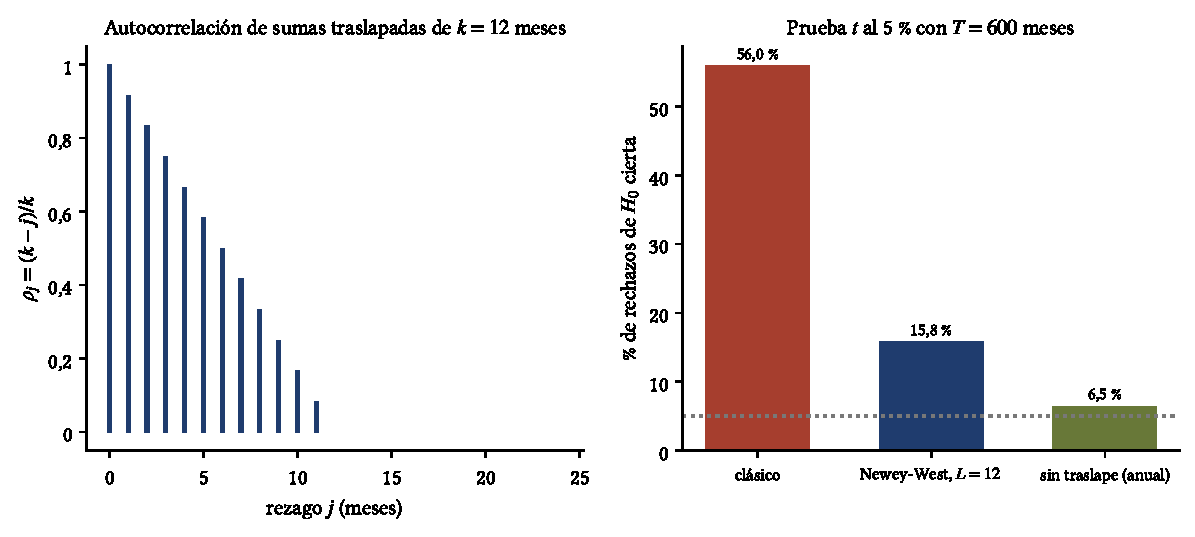
\includegraphics[width=\linewidth]{graficos/cap04_fig_traslape.pdf}
\caption{Izquierda: autocorrelación teórica de rendimientos de 12 meses calculados cada mes; decrece en línea
recta hasta anularse en el rezago 12 (Proposición~\ref{prop:traslape}). Derecha: porcentaje de rechazos de
$H_0:\beta=0$, que es cierta, al regresar rendimientos traslapados sobre un predictor independiente y muy
persistente ($\phi=0{,}98$), en 2\,000 simulaciones con $T=600$.}
\label{fig:traslape}
\end{figure}

\begin{observacion}
Las regresiones predictivas con predictores muy persistentes tienen además otro problema, el \emph{sesgo
de Stambaugh} (1999): si las innovaciones del predictor están correlacionadas con las del rendimiento, como
ocurre con la razón dividendo/precio, $\hat\beta$ está sesgado en muestras finitas. Lo retomaremos en el
Capítulo~6.
\end{observacion}

% ---------------------------------------------------------------------
\section{Cambios estructurales}
% ---------------------------------------------------------------------

En setenta años pueden cambiar la regulación, la tecnología y la composición de las empresas de un sector.
Si la beta cambió y estimamos una sola recta, obtenemos un promedio de dos regímenes que no describe ninguno
de ellos (Figura~\ref{fig:quiebre}).

\begin{figure}[ht]
\centering
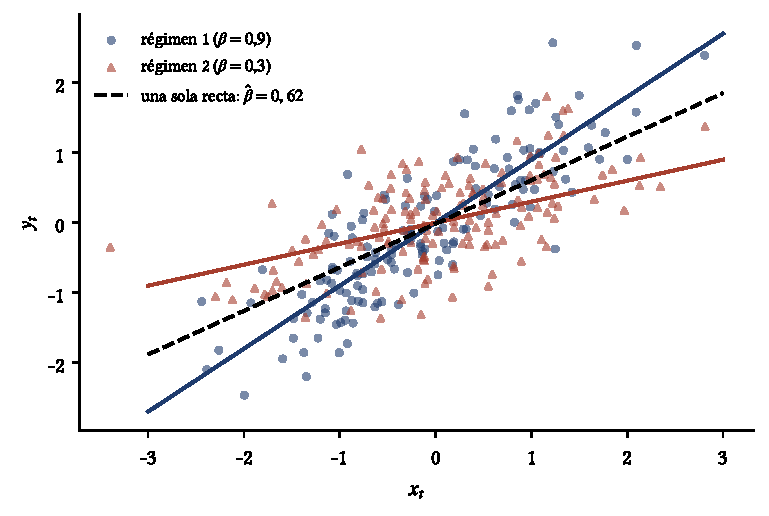
\includegraphics[width=0.66\linewidth]{graficos/cap04_fig_quiebre.pdf}
\caption{Datos simulados con un cambio de régimen: la pendiente es 0,9 en el primero (círculos) y 0,3 en el
segundo (triángulos). Una sola recta (línea discontinua) da una pendiente intermedia de 0,62, que no
representa ninguno de los dos regímenes.}
\label{fig:quiebre}
\end{figure}

\begin{definicion}[Prueba de Chow]
Para una fecha de quiebre conocida $\tau$, se estima el modelo con toda la muestra (suma de residuos al
cuadrado $\mathrm{SRC}$) y por separado antes y después de $\tau$ ($\mathrm{SRC}_1$ y $\mathrm{SRC}_2$). Con $k$
parámetros por régimen,
\[
  F=\frac{(\mathrm{SRC}-\mathrm{SRC}_1-\mathrm{SRC}_2)/k}{(\mathrm{SRC}_1+\mathrm{SRC}_2)/(T-2k)} .
\]
Con errores normales, homocedásticos y no correlacionados, $F$ sigue una distribución $F_{k,\,T-2k}$ bajo la
hipótesis nula de que los parámetros no cambiaron.
\end{definicion}

La prueba de Chow equivale a estimar un solo modelo con una variable indicadora $D_t=\mathbb 1\{t\ge\tau\}$
y sus interacciones con los regresores, y a probar que los coeficientes de esos términos son cero. Esta
forma permite usar errores robustos: se calcula la prueba de Wald con la matriz HC1 o Newey-West, y se compara
con una $\chi^2_k$.

\paragraph{Fecha desconocida.} Si la fecha se elige mirando los datos, por ejemplo donde $F$ es máximo, los
valores críticos de la $F$ ya no sirven: el máximo de muchas $F$ es mucho mayor que una $F$ típica. Andrews
(1993) obtuvo la distribución asintótica de $\sup F$ sobre las fechas entre el 15\,\% y el 85\,\% de la
muestra. Para $k=2$, el valor crítico al 5\,\% del estadístico de Wald ($=k\cdot\sup F$) es de
aproximadamente 11,8; nuestra simulación con puentes brownianos da 11,70, es decir, $\sup F$ crítico
$\approx5{,}85$ (Ejercicio propuesto~4.6).

\paragraph{CUSUM.} Brown, Durbin y Evans (1975) propusieron vigilar la estabilidad con los \emph{residuos
recursivos}: el error de pronóstico de $y_t$ con el modelo estimado hasta $t-1$, estandarizado,
\[
  w_t=\frac{y_t-\bm x_t'\hat{\bm\beta}_{t-1}}{\sqrt{1+\bm x_t'(\bm X_{t-1}'\bm X_{t-1})^{-1}\bm x_t}} .
\]
Con errores normales e i.i.d. y parámetros estables, los $w_t$ son i.i.d. $N(0,\sigma^2)$. Su suma acumulada
estandarizada, $W_t=\sum_{s\le t}w_s/\hat\sigma_w$, se mueve como un paseo aleatorio alrededor de cero; un
cambio en los parámetros produce errores de pronóstico sistemáticos y $W_t$ se desvía. Las bandas al 5\,\%
son $\pm0{,}948\bigl[\sqrt{T-k}+2(t-k)/\sqrt{T-k}\bigr]$.

% ---------------------------------------------------------------------
\section{Ejercicios resueltos}
% ---------------------------------------------------------------------

\begin{ejresuelto}{Heterocedasticidad en la beta de los servicios públicos}\label{ej:white}
\enunciado Con el modelo de mercado de \texttt{Utils} (Ejercicio~\ref{ej:utils}): (a) aplique las pruebas de
Breusch-Pagan y de White; (b) calcule los errores estándar clásicos, HC0 y HC1 con la matriz sándwich;
(c) repita las pruebas de $\alpha=0$ y $\beta=1$.

\solucion
\paso{Paso 1. Pruebas.} Breusch-Pagan: $LM=6{,}19$ con 1 grado de libertad, $p=0{,}013$. White:
$LM=36{,}56$ con 2 grados de libertad, $p\approx10^{-8}$. Las dos rechazan la homocedasticidad, pero la de
White con mucha más fuerza: la Figura~\ref{fig:white} muestra que los residuos al cuadrado crecen tanto
con las subidas como con las caídas del mercado, una relación en forma de U que solo el término $x_t^2$ capta.

\paso{Paso 2. Errores estándar.} Para $\hat\beta$: clásico $0{,}02497$, HC0 $0{,}03312$ y HC1 $0{,}03316$.
El cociente entre el robusto y el clásico es
\begin{align*}
  \frac{\operatorname{ee}_{\mathrm{HC1}}(\hat\beta)}{\operatorname{ee}_{\text{clásico}}(\hat\beta)}
    &= \frac{0{,}03316}{0{,}02497}\\
    &= 1{,}328 :
\end{align*}
el error estándar robusto es un 33\,\% mayor. Para $\hat\alpha$ el cambio es mínimo ($0{,}00107$ a
$0{,}00110$), porque la constante no interactúa con la forma de la heterocedasticidad.

\paso{Paso 3. Pruebas revisadas.} Con los errores HC1:
\begin{align*}
  t_{\mathrm{HC1}}(\beta=1)  &= \frac{0{,}54087-1}{0{,}03316}\\
                             &= -13{,}85,\\
  t_{\mathrm{HC1}}(\alpha=0) &= \frac{0{,}0024625}{0{,}0011043}\\
                             &= 2{,}23 .
\end{align*}
La beta sigue siendo claramente menor que 1 (antes, $t=-18{,}39$) y la alfa sigue siendo significativa al
5\,\% (antes, $t=2{,}30$).

\codigoweb{cap04_ej01}
\salidaR{cap04_ej01_R.txt}
\lectura{cap04_ej01}

\RvsPy Programamos la matriz sándwich en ambos lenguajes para que el cálculo sea transparente. La
expresión \texttt{X * e} multiplica cada fila de $\bm X$ por su residuo: en R funciona porque el vector
\texttt{e} se recicla por columnas; en NumPy hay que convertirlo en columna con \texttt{e[:, None]}. En la
práctica, R ofrece estas matrices en el paquete \texttt{sandwich} y Python en la opción \texttt{cov\_type}
de \texttt{statsmodels}, que usamos como comprobación.

\begin{figure}[ht]
\centering
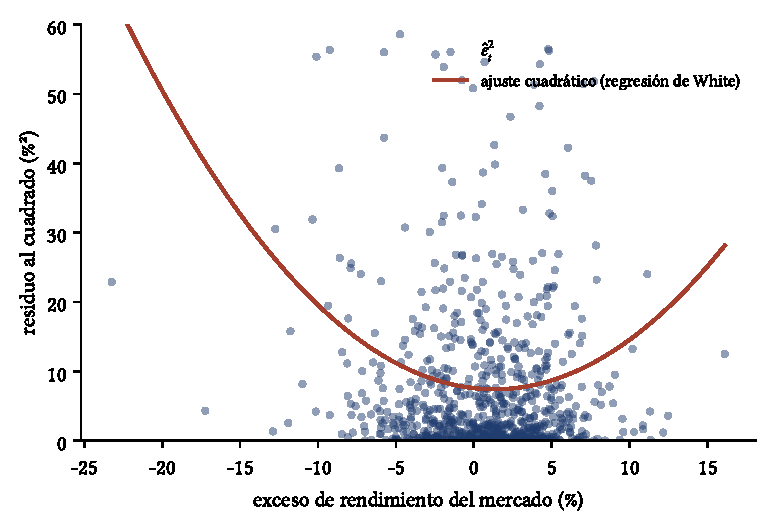
\includegraphics[width=0.68\linewidth]{graficos/cap04_fig_white.pdf}
\caption{Residuos al cuadrado del modelo de mercado de \texttt{Utils} frente al exceso de rendimiento del
mercado. La parábola ajustada (la regresión auxiliar de White) muestra que la varianza del residuo crece en
ambos extremos.}
\label{fig:white}
\end{figure}

\begin{conclusion}
Hay heterocedasticidad clara, y los errores estándar clásicos de la beta la subestiman en un tercio. Las
conclusiones del Capítulo~\ref{cap:capm} sobre \texttt{Utils} se mantienen, pero con menos holgura de la que
parecía.
\end{conclusion}
\end{ejresuelto}

\begin{ejresuelto}{¿Sobreviven las alfas del CAPM a los errores robustos?}\label{ej:alfasrob}
\enunciado Repita el Ejercicio~\ref{ej:industrias} con errores HC1 y Newey-West ($L=6$). ¿Cuántas alfas
siguen siendo significativas? ¿Cuánto crecen los errores estándar de las betas?

\solucion
\paso{Paso 1. Rezagos.} Con $T=819$, la regla de Newey y West da
\begin{align*}
  L &= \Bigl\lfloor 4\Bigl(\frac{T}{100}\Bigr)^{2/9}\Bigr\rfloor\\
    &= \bigl\lfloor 4\,(8{,}19)^{2/9}\bigr\rfloor\\
    &= \lfloor 4\times1{,}5957\rfloor\\
    &= \lfloor 6{,}38\rfloor\\
    &= 6 .
\end{align*}

\paso{Paso 2. Alfas.} Las cuatro alfas significativas con errores clásicos siguen siéndolo con HC1 y con
Newey-West: \texttt{NoDur} (de $t=2{,}87$ a $2{,}27$ con Newey-West), \texttt{Hlth} (de $2{,}49$ a
$2{,}32$), \texttt{Utils} (de $2{,}30$ a $2{,}25$) y \texttt{Other} (de $-2{,}24$ a $-2{,}16$). La evidencia
contra el CAPM del Capítulo~\ref{cap:capm} no era un artefacto de los errores estándar.

\paso{Paso 3. Betas.} Los errores estándar de las betas crecen mucho más: en promedio, el de Newey-West es
1,6 veces el clásico, y en \texttt{NoDur} es el doble. Newey-West supera a HC1 en las doce industrias,
lo que indica que los productos $x_t\hat\varepsilon_t$ están autocorrelacionados: es la huella del
agrupamiento de volatilidad. Con estos errores, \texttt{Money} ($t(\beta=1)=1{,}61$) se suma a
\texttt{Shops} como industria cuya beta no se distingue de 1.

\codigoweb{cap04_ej02}
\salidaR{cap04_ej02_R.txt}
\lectura{cap04_ej02}

\RvsPy Para que Python reproduzca la fórmula de Newey-West sin correcciones adicionales hay que indicar
\texttt{use\_correction=False} en \texttt{statsmodels}; por defecto multiplica la matriz por $T/(T-k)$. Es
un buen ejemplo de por qué conviene saber qué calcula cada función: las dos versiones son válidas, pero
difieren en la tercera cifra decimal.

\begin{figure}[ht]
\centering
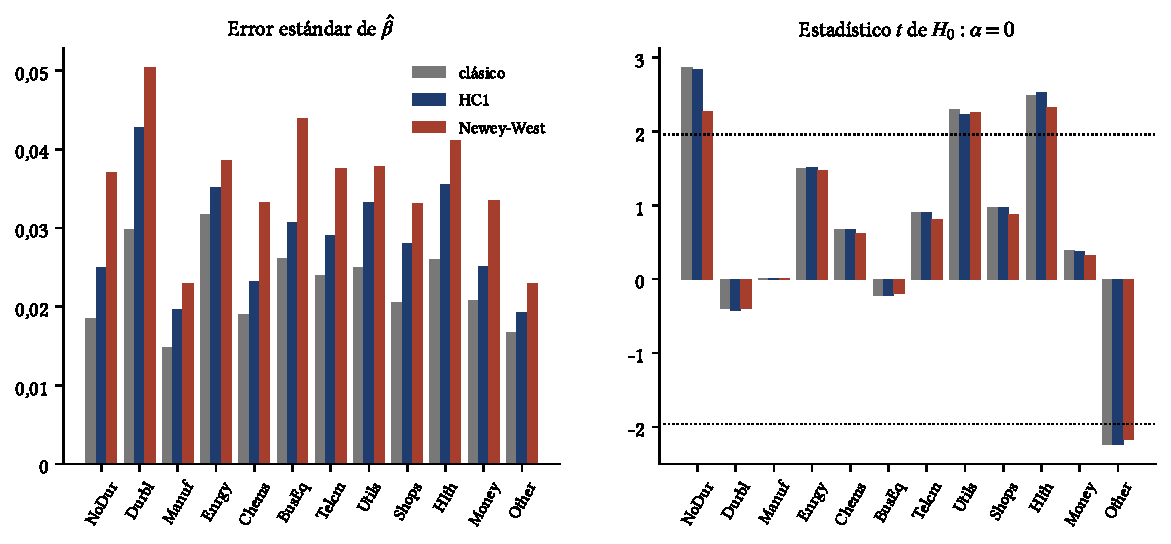
\includegraphics[width=\linewidth]{graficos/cap04_fig_robustos.pdf}
\caption{Izquierda: error estándar de $\hat\beta$ con los tres métodos; el de Newey-West es el mayor en todas
las industrias. Derecha: estadístico $t$ de $\alpha=0$; las barras que superan las líneas punteadas
($\pm1{,}96$) son las mismas con los tres métodos.}
\label{fig:robustos}
\end{figure}

\begin{conclusion}
Los errores robustos no cambian las conclusiones sobre las alfas, pero sí la precisión con que conocemos las
betas, que es un 60\,\% menor de lo que indicaban los errores clásicos. En aplicaciones financieras, los
errores HAC deberían ser la opción por defecto.
\end{conclusion}
\end{ejresuelto}

\begin{ejresuelto}{La deuda del Capítulo 2: autocorrelación del Brent con bandas robustas}\label{ej:acfrob}
\enunciado Con los rendimientos diarios del Brent, calcule las diez primeras autocorrelaciones con las bandas
de Bartlett y con las bandas robustas de la Proposición~\ref{prop:acfrob}. Compare la prueba de Ljung-Box con
la versión robusta $Q^*(10)$.

\solucion
\paso{Paso 1. Bandas.} La banda de Bartlett es $\pm0{,}0205$ en todos los rezagos. Las robustas van de
$\pm0{,}038$ (rezago 8) a $\pm0{,}090$ (rezago 1): entre 1,9 y 4,4 veces más anchas.

\paso{Paso 2. Rezagos ``significativos''.} Con la banda clásica, los rezagos 2, 8 y 10 parecían
significativos ($t=-2{,}47$; $1{,}98$; $-2{,}69$). Con la robusta, sus estadísticos son $-1{,}12$; $1{,}07$ y
$-0{,}87$: ninguno se acerca a la significancia.

\paso{Paso 3. Prueba conjunta.} Ljung-Box da $Q(10)=25{,}74$, $p=0{,}0041$; la versión robusta da
$Q^*(10)=4{,}67$, $p=0{,}912$.

\codigoweb{cap04_ej03}
\salidaR{cap04_ej03_R.txt}
\lectura{cap04_ej03}

\RvsPy Los dos programas siguen exactamente las fórmulas de la Proposición~\ref{prop:acfrob} sobre los
rendimientos centrados. En R convertimos el resultado de \texttt{sapply} en un \texttt{data.frame} para
acceder a las columnas por nombre (\texttt{res\$rho}).

\begin{figure}[ht]
\centering
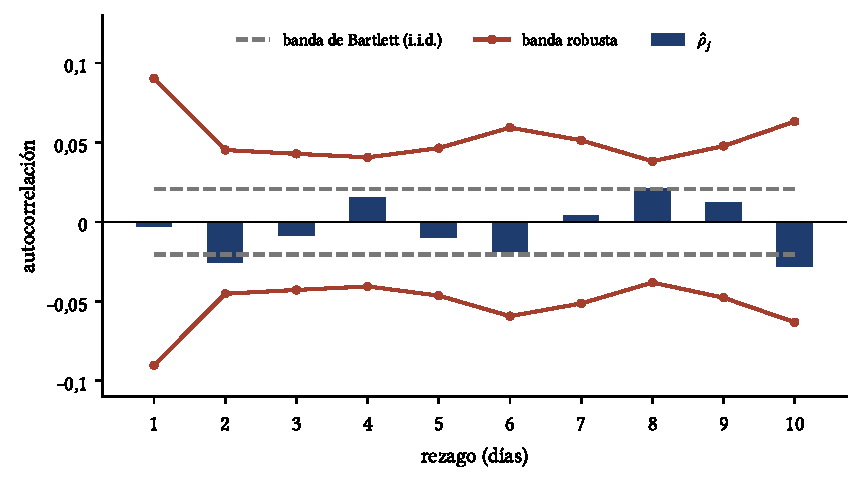
\includegraphics[width=0.78\linewidth]{graficos/cap04_fig_acfrobusta.pdf}
\caption{Autocorrelaciones del Brent con la banda de Bartlett (gris), válida solo con datos i.i.d., y con la
banda robusta (roja). Ninguna autocorrelación sale de la banda robusta.}
\label{fig:acfrobusta}
\end{figure}

\begin{conclusion}
El rechazo de Ljung-Box en el Capítulo~\ref{cap:hechos} era un artefacto del agrupamiento de volatilidad. Con
inferencia válida, no hay evidencia de autocorrelación en los rendimientos diarios del Brent, en línea con la
eficiencia débil del mercado petrolero, que estudiaremos en el Capítulo~7.
\end{conclusion}
\end{ejresuelto}

\begin{ejresuelto}{¿Predice la razón dividendo/precio el rendimiento bursátil?}\label{ej:dprediccion}
\enunciado Con el S\&P 500 de Shiller (1871--2023), regrese el rendimiento total logarítmico de los próximos
12 meses sobre $\ln(D_t/P_t)$, usando todos los meses (datos traslapados). Compare los errores estándar
clásicos, de Newey-West con $L=12$ y $L=24$, y la regresión con un solo dato por año (eneros, sin traslape).

\solucion
\paso{Paso 1. Estimación.} Con 1\,818 meses (enero de 1871 a junio de 2022 como fechas iniciales),
$\hat b=0{,}0412$ y $R^2=0{,}0107$. El signo es el que predice la teoría (Campbell y Shiller, 1988): cuando los
precios están altos en relación con los dividendos, los rendimientos futuros tienden a ser menores.

\paso{Paso 2. Inferencia.} Con errores clásicos, $t=4{,}43$: predictibilidad ``muy significativa''. Con
Newey-West, $t=1{,}46$ ($L=12$) y $t=1{,}35$ ($L=24$). Sin traslape, con 152 eneros, $\hat b=0{,}0334$ y
$t=1{,}09$. Ninguna versión válida es significativa al 5\,\%.

\paso{Paso 3. Comparación con la teoría.} La razón dividendo/precio es extremadamente persistente: su
autocorrelación es $0{,}996$ al primer rezago y $0{,}906$ a los doce meses. Con $\rho_x(j)=0{,}996^{\,j}$ y
$\rho_\varepsilon(j)=(12-j)/12$, la Proposición~\ref{prop:inflacion} da
\begin{align*}
  1+2\sum_{j=1}^{11}0{,}996^{\,j}\,\frac{12-j}{12} &= 1+2\times5{,}406\\
                                                    &= 11{,}81,\\
  \sqrt{11{,}81}                                    &= 3{,}44 .
\end{align*}
Los errores estándar verdaderos deberían ser unas 3,44 veces los clásicos. En los datos,
\begin{align*}
  \frac{\operatorname{ee}_{\mathrm{NW}}(\hat b)}{\operatorname{ee}_{\text{clásico}}(\hat b)} &= \frac{0{,}0283}{0{,}0093}\\
                                                                                         &= 3{,}04 :
\end{align*}
la teoría explica casi todo el desajuste.

\codigoweb{cap04_ej04}
\salidaR{cap04_ej04_R.txt}
\lectura{cap04_ej04}

\RvsPy La serie de Shiller incluye los dividendos anuales acumulados de cada mes; el rendimiento mensual
total suma la doceava parte al precio. En los dos lenguajes cortamos la muestra en junio de 2023, último mes
con dividendo publicado; si no se hace, los dividendos iguales a cero producen $\ln 0=-\infty$ y la regresión
falla o, peor, descarta observaciones sin avisar.

\begin{figure}[ht]
\centering
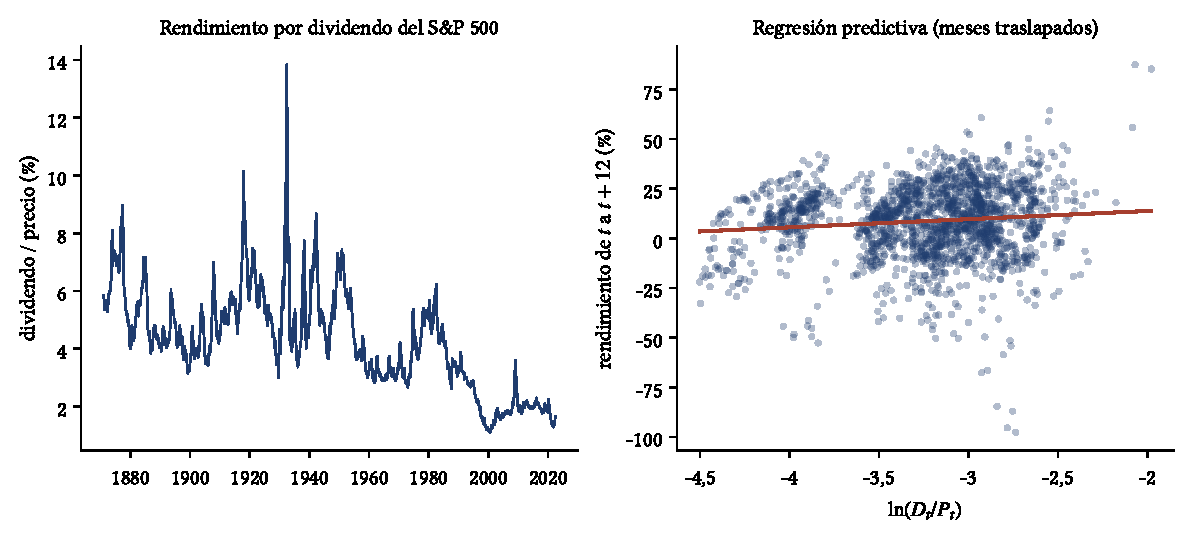
\includegraphics[width=\linewidth]{graficos/cap04_fig_dividendos.pdf}
\caption{Izquierda: rendimiento por dividendo del S\&P 500, una serie muy persistente que tocó su
mínimo histórico (1,1\,\% en agosto de 2000). Derecha: rendimiento de los 12 meses siguientes frente al logaritmo de la razón
dividendo/precio. La pendiente positiva es pequeña frente a la dispersión, y los puntos vecinos no son
observaciones independientes.}
\label{fig:dividendos}
\end{figure}

\begin{conclusion}
La aparente predictibilidad del mercado accionario con la razón dividendo/precio desaparece cuando se corrige
la inferencia por el traslape. Sumado al sesgo de Stambaugh, este ejemplo muestra por qué la literatura sobre
predictibilidad de rendimientos exige errores HAC, pruebas sin traslape y evaluación fuera de muestra.
\end{conclusion}
\end{ejresuelto}

\begin{ejresuelto}{¿Cambió la beta de los servicios públicos tras la desregulación eléctrica?}\label{ej:chow}
\enunciado En octubre de 1992 se promulgó en EE.\,UU. la Ley de Política Energética, que abrió a la
competencia la generación eléctrica mayorista. Con el modelo de mercado de \texttt{Utils}: (a) aplique la
prueba de Chow con quiebre en octubre de 1992 y su versión robusta; (b) calcule $\sup F$ sin fijar la fecha;
(c) aplique la prueba CUSUM.

\solucion
\paso{Paso 1. Chow.} $F=11{,}43$ frente a un valor crítico de $F_{2,815}$ al 5\,\% de $3{,}01$ ($p=1{,}3\times10^{-5}$).
La beta pasa de $0{,}629$ antes de la ley a $0{,}384$ después, y la alfa anual, de $2{,}19$\,\% a $4{,}35$\,\%.
Como hay heterocedasticidad (Ejercicio~\ref{ej:white}), repetimos con la prueba de Wald robusta: $W=10{,}97$
frente a $\chi^2_2=5{,}99$, $p=0{,}004$. El cambio se confirma.

\paso{Paso 2. Fecha desconocida.} El máximo de las $F$ entre el 15\,\% y el 85\,\% de la muestra es
$16{,}69$, en febrero de 1987, muy por encima del valor crítico de Andrews ($\approx5{,}85$). La
Figura~\ref{fig:quiebres} muestra que la $F$ supera el valor crítico en casi todas las fechas entre abril de
1974 y noviembre de 1999: la beta cambió en algún momento de ese período, pero los datos no permiten
fecharlo con precisión, y octubre de 1992 no es la fecha más probable. Sospechar una ley concreta no basta
para atribuirle el cambio.

\paso{Paso 3. CUSUM.} El estadístico nunca cruza sus bandas: su máximo llega al 73\,\% de la banda. La prueba
no detecta el cambio que Chow y $\sup F$ detectan con claridad. No es una contradicción: CUSUM acumula errores
de pronóstico, que se vuelven sistemáticos cuando cambia el nivel de la serie; un cambio en la pendiente con
un regresor de media cercana a cero (el exceso del mercado) produce errores que se compensan entre meses
buenos y malos, y la suma apenas se mueve (Ploberger y Krämer, 1990).

\codigoweb{cap04_ej05}
\salidaR{cap04_ej05_R.txt}
\lectura{cap04_ej05}

\RvsPy Dos trampas de índices. Primero, la fecha de quiebre: en R, \texttt{tb} es la posición (desde 1) del
primer mes del segundo régimen; en Python, la misma fecha es \texttt{tb} desde 0, y los cortes
\texttt{slice(0, tb)} y \texttt{slice(tb, T)} la dejan en el segundo régimen. Segundo, \texttt{np.argmax}
aplicado a un vector sin ningún \texttt{True} devuelve 0, no un aviso: la primera versión de nuestro código
reportaba un cruce falso en marzo de 1949 hasta que lo corregimos.

\begin{figure}[ht]
\centering
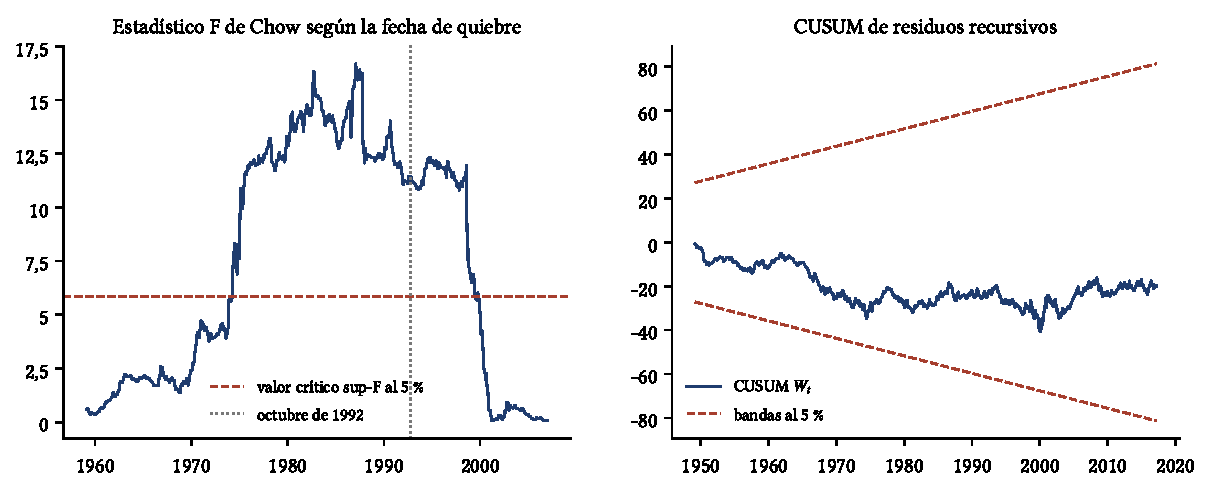
\includegraphics[width=\linewidth]{graficos/cap04_fig_quiebres.pdf}
\caption{Izquierda: estadístico $F$ de Chow para cada fecha posible, con el valor crítico de $\sup F$ al 5\,\%
(línea discontinua) y octubre de 1992 (línea punteada). Derecha: CUSUM de residuos recursivos con sus bandas
al 5\,\%; el estadístico se aleja de cero, pero no las cruza.}
\label{fig:quiebres}
\end{figure}

\begin{conclusion}
La beta de los servicios públicos cayó de forma significativa entre la primera y la segunda mitad de la
muestra, de 0,63 a 0,38, pero la fecha exacta no está bien identificada. Cada prueba responde una pregunta
distinta: Chow evalúa una fecha elegida de antemano, $\sup F$ busca la fecha en los datos con valores
críticos adecuados y CUSUM vigila sobre todo cambios de nivel.
\end{conclusion}
\end{ejresuelto}

% ---------------------------------------------------------------------
\section{Ejercicios propuestos}
% ---------------------------------------------------------------------

\begin{enumerate}[label=\textbf{\thechapter.\arabic*},leftmargin=*,itemsep=6pt]
  \item Demuestre que si $\sigma_t^2$ no está correlacionada con $(x_t-\bar x)^2$, el cociente de la
  Proposición~\ref{prop:mcohetero} es 1, aunque haya heterocedasticidad. ¿Por qué entonces los errores
  robustos de $\hat\alpha$ casi no cambian en el Ejercicio~\ref{ej:white}?

  \item Demuestre que el estimador de Newey-West con $L=1$ es semidefinido positivo en el caso escalar.
  \textit{Pista: escríbalo como $\frac12\sum_t(\hat u_t+\hat u_{t-1})^2$ más términos no negativos.}

  \item Use la Proposición~\ref{prop:inflacion} para calcular el factor de inflación con $k=12$ y
  $\rho_x(j)=\phi^j$ para $\phi=0{,}5;\ 0{,}9;\ 0{,}99$. \textit{Respuesta: 2,67; 8,24 y 11,54.}

  \item Demuestre que la prueba de Chow equivale a la prueba $F$ de que los coeficientes de $D_t$ y
  $D_t\,x_t$ son cero en la regresión con interacciones.

  \item \emph{(Simulación.)} Modifique el código de \texttt{cap04\_figuras\_teoria.py} para que los errores
  sigan un ARCH(1) con $a=0{,}5$ y el regresor sea i.i.d. normal. ¿Cuánto rechaza la prueba $t$ clásica de
  $\beta=0$? ¿Y la prueba con errores HC1?

  \item \emph{(Simulación.)} Simule el valor crítico de $\sup F$ de Andrews: genere dos movimientos
  brownianos independientes en una malla de 2\,000 puntos, construya los puentes $B(\pi)=W(\pi)-\pi W(1)$ y
  calcule $\sup_{\pi\in[0{,}15;\,0{,}85]}\|B(\pi)\|^2/[\pi(1-\pi)]$. Con 20\,000 repeticiones, el cuantil del
  95\,\% debe estar cerca de 11,7 a 11,8.

  \item \emph{(Con datos.)} Repita el Ejercicio~\ref{ej:dprediccion} con dos submuestras, 1871--1945 y
  1946--2022. ¿Es significativa la pendiente en alguna de ellas con Newey-West? ¿Por qué no basta un
  estadístico $t$ alto en la segunda submuestra para concluir que hay predictibilidad?

  \item \emph{(Con datos del BCRP.)} Estime la beta de una acción peruana respecto del índice de la BVL con
  errores clásicos, HC1 y Newey-West, y aplique la prueba de Chow con quiebre en marzo de 2020 (inicio de la
  emergencia sanitaria). ¿Cambió la beta?
\end{enumerate}

% ---------------------------------------------------------------------
\section{Resumen de fórmulas}
% ---------------------------------------------------------------------

\begin{table}[H]
\centering\small
\begin{tabular}{@{}ll@{}}
\toprule
Concepto & Fórmula \\
\midrule
Varianza de MCO (sándwich) & $(\bm X'\bm X)^{-1}\bigl(\sum_t\sigma_t^2\bm x_t\bm x_t'\bigr)(\bm X'\bm X)^{-1}$ \\
White (HC0, HC1) & $\sigma_t^2\to\hat\varepsilon_t^2$;\quad HC1 $=\frac{T}{T-k}$HC0 \\
Breusch-Pagan, White & $LM=T\,R^2_{\mathrm{aux}}\xrightarrow{d}\chi^2_q$ \\
Varianza de largo plazo & $\bm S=\bm\Gamma_0+\sum_{j\ge1}(\bm\Gamma_j+\bm\Gamma_j')$ \\
Newey-West & pesos $1-j/(L+1)$;\quad $L=\lfloor4(T/100)^{2/9}\rfloor$ \\
Autocorrelación robusta & $\hat v_j=\sum_tr_t^2r_{t-j}^2/(\sum_tr_t^2)^2$;\quad $Q^*(m)=\sum_j\hat\rho_j^2/\hat v_j$ \\
Traslape de $k$ períodos & $\rho(j)=(k-j)/k$;\quad inflación $\approx1+2\sum_j\rho_x(j)\rho_\varepsilon(j)$ \\
Chow & $F=\frac{(\mathrm{SRC}-\mathrm{SRC}_1-\mathrm{SRC}_2)/k}{(\mathrm{SRC}_1+\mathrm{SRC}_2)/(T-2k)}$ \\
CUSUM & bandas $\pm0{,}948\bigl[\sqrt{T-k}+2(t-k)/\sqrt{T-k}\bigr]$ \\
\bottomrule
\end{tabular}
\caption{Fórmulas principales del Capítulo 4.}
\end{table}

\section*{Referencias}
\begin{itemize}[leftmargin=*]
  \item Andrews, D. W. K. (1993). Tests for parameter instability and structural change with unknown change
        point. \emph{Econometrica}, 61(4), 821--856.
  \item Breusch, T. S. y Pagan, A. R. (1979). A simple test for heteroscedasticity and random coefficient
        variation. \emph{Econometrica}, 47(5), 1287--1294.
  \item Brown, R. L., Durbin, J. y Evans, J. M. (1975). Techniques for testing the constancy of regression
        relationships over time. \emph{Journal of the Royal Statistical Society, Series B}, 37(2), 149--192.
  \item Campbell, J. Y. y Shiller, R. J. (1988). The dividend-price ratio and expectations of future
        dividends and discount factors. \emph{The Review of Financial Studies}, 1(3), 195--228.
  \item Chow, G. C. (1960). Tests of equality between sets of coefficients in two linear regressions.
        \emph{Econometrica}, 28(3), 591--605.
  \item Koenker, R. (1981). A note on studentizing a test for heteroscedasticity. \emph{Journal of
        Econometrics}, 17(1), 107--112.
  \item Lobato, I., Nankervis, J. C. y Savin, N. E. (2001). Testing for autocorrelation using a modified
        Box-Pierce Q test. \emph{International Economic Review}, 42(1), 187--205.
  \item Newey, W. K. y West, K. D. (1987). A simple, positive semi-definite, heteroskedasticity and
        autocorrelation consistent covariance matrix. \emph{Econometrica}, 55(3), 703--708.
  \item Newey, W. K. y West, K. D. (1994). Automatic lag selection in covariance matrix estimation.
        \emph{The Review of Economic Studies}, 61(4), 631--653.
  \item Ploberger, W. y Krämer, W. (1990). The local power of the CUSUM and CUSUM of squares tests.
        \emph{Econometric Theory}, 6(3), 335--347.
  \item Stambaugh, R. F. (1999). Predictive regressions. \emph{Journal of Financial Economics}, 54(3),
        375--421.
  \item White, H. (1980). A heteroskedasticity-consistent covariance matrix estimator and a direct test for
        heteroskedasticity. \emph{Econometrica}, 48(4), 817--838.
\end{itemize}

% =====================================================================
%  Capítulo 5. Estacionariedad y raíces unitarias
% =====================================================================
\part{Series de tiempo univariadas}

\chapter[Estacionariedad y raíces unitarias]{Estacionariedad, autocorrelación y raíces unitarias}\label{cap:raiz}

\section*{Objetivos de aprendizaje}
Al terminar este capítulo, el lector podrá:
\begin{enumerate}[label=\arabic*.,leftmargin=*]
  \item Definir la estacionariedad y distinguir un proceso estacionario de uno con raíz unitaria por sus
        momentos, sus trayectorias y su función de autocorrelación.
  \item Calcular la persistencia de un proceso autorregresivo con la vida media de un choque.
  \item Explicar por qué una regresión entre series con raíz unitaria puede ser espuria.
  \item Derivar la distribución de Dickey-Fuller y aplicar las pruebas ADF y KPSS con la especificación
        determinista y el número de rezagos adecuados.
  \item Reconocer el efecto de los quiebres estructurales sobre las pruebas de raíz unitaria y aplicar la
        prueba de Zivot-Andrews.
\end{enumerate}

\section*{Motivación}
¿Vuelve el precio del petróleo a un nivel ``normal'' después de una crisis, o cada choque lo deja en un
nivel nuevo, del que parte la siguiente historia? ¿Regresa el miedo del mercado, medido por el VIX, a su
promedio? ¿Fluctúan las tasas de interés de largo plazo alrededor de un valor estable o deambulan sin
ancla? La respuesta a estas preguntas determina casi todo lo que se puede hacer con una serie: si tiene
sentido pronosticarla a largo plazo, si se puede usar en una regresión sin transformar, si sus choques
son transitorios o permanentes.

La herramienta para responderlas es la distinción entre series \emph{estacionarias} y series con
\emph{raíz unitaria}, y las pruebas que permiten decidir entre ambas. Este capítulo abre la Parte~II del
libro: a partir de aquí los datos dejan de ser muestras de observaciones independientes y pasan a ser lo
que realmente son en finanzas: trayectorias en el tiempo.

\paragraph{Datos del capítulo.} Brent diario (1987--2026), VIX diario (1990--2026), tasa de interés del bono
del Tesoro de EE.\,UU. a 10 años y razón dividendo/precio del S\&P 500 (base de Shiller, 1871--2023), y
precio mensual del oro (1975--2026).

% ---------------------------------------------------------------------
\section{Procesos estocásticos y estacionariedad}
% ---------------------------------------------------------------------

Una serie de tiempo $y_1,\dots,y_T$ se interpreta como una realización de un \emph{proceso estocástico}
$\{y_t\}$: una sucesión de variables aleatorias indexadas por el tiempo. Solo observamos una trayectoria;
para aprender algo del proceso a partir de ella, sus propiedades deben ser estables en el tiempo.

\begin{definicion}[Estacionariedad débil]
El proceso $\{y_t\}$ es \emph{débilmente estacionario} (o estacionario en covarianza) si para todo $t$ y todo
$j$:
\begin{align*}
  \E[y_t]            &= \mu,\\
  \Var(y_t)          &= \gamma_0<\infty,\\
  \Cov(y_t,y_{t-j})  &= \gamma_j,
\end{align*}
es decir, la media, la varianza y las autocovarianzas no dependen de $t$, sino solo de la distancia $j$.
La \emph{función de autocorrelación} (ACF) es $\rho_j=\gamma_j/\gamma_0$.
\end{definicion}

\begin{definicion}[Ruido blanco]
Un proceso $\{\varepsilon_t\}$ es \emph{ruido blanco} si tiene media cero, varianza constante $\sigma^2$ y
autocovarianzas nulas: $\gamma_j=0$ para $j\ne0$. Si además las $\varepsilon_t$ son independientes, es ruido
blanco i.i.d. Los rendimientos del Brent del Capítulo~\ref{cap:hechos} son ruido blanco, pero no i.i.d.
\end{definicion}

\begin{definicion}[Autocorrelación parcial]
La \emph{autocorrelación parcial} (PACF) de orden $j$, $\phi_{jj}$, es el último coeficiente de la regresión
poblacional de $y_t$ sobre $y_{t-1},\dots,y_{t-j}$: mide la relación entre $y_t$ y $y_{t-j}$ una vez
descontado el efecto de los rezagos intermedios.
\end{definicion}

\subsection{El proceso autorregresivo de orden 1}

\begin{definicion}[AR(1)]
$y_t=c+\phi\,y_{t-1}+\varepsilon_t$, con $\varepsilon_t$ ruido blanco de varianza $\sigma^2$.
\end{definicion}

\begin{proposicion}[Momentos del AR(1) estacionario]\label{prop:ar1}
Si $|\phi|<1$ y el proceso es estacionario, entonces
\begin{align*}
  \mu      &= \frac{c}{1-\phi},\\
  \gamma_0 &= \frac{\sigma^2}{1-\phi^2},\\
  \rho_j   &= \phi^{\,j}, \qquad j\ge0 .
\end{align*}
\end{proposicion}

\begin{proof}
\emph{Media.} Tomando esperanzas y usando $\E[y_t]=\E[y_{t-1}]=\mu$:
\begin{align*}
  \mu           &= c+\phi\,\mu\\
  \mu-\phi\,\mu &= c\\
  \mu           &= \frac{c}{1-\phi}.
\end{align*}
\emph{Varianza.} Como $\varepsilon_t$ no está correlacionado con $y_{t-1}$, que solo depende de choques
pasados, y $\Var(y_t)=\Var(y_{t-1})=\gamma_0$:
\begin{align*}
  \gamma_0               &= \Var(c+\phi\,y_{t-1}+\varepsilon_t)\\
                         &= \phi^2\,\gamma_0+\sigma^2\\
  \gamma_0\,(1-\phi^2)   &= \sigma^2\\
  \gamma_0               &= \frac{\sigma^2}{1-\phi^2}.
\end{align*}
\emph{Autocovarianzas.} Para $j\ge1$, $\varepsilon_t$ no está correlacionado con $y_{t-j}$:
\begin{align*}
  \gamma_j &= \Cov(y_t,\,y_{t-j})\\
           &= \Cov(c+\phi\,y_{t-1}+\varepsilon_t,\ y_{t-j})\\
           &= \phi\,\Cov(y_{t-1},\,y_{t-j})\\
           &= \phi\,\gamma_{j-1}.
\end{align*}
Aplicando la recursión $j$ veces, $\gamma_j=\phi^{\,j}\gamma_0$, y dividiendo entre $\gamma_0$,
$\rho_j=\phi^{\,j}$.
\end{proof}

La ACF de un AR(1) estacionario decae geométricamente: rápido si $\phi$ es pequeño, lentamente si $\phi$ se
acerca a 1. Su PACF, en cambio, se corta después del primer rezago, porque una vez conocido $y_{t-1}$ los
rezagos anteriores no aportan información sobre $y_t$. La Figura~\ref{fig:procesos} muestra cómo cambia la
trayectoria al aumentar $\phi$.

\begin{proposicion}[Vida media de un choque]\label{prop:vidamedia}
En un AR(1) estacionario con $0<\phi<1$, el efecto de un choque sobre $y_{t+h}$ es $\phi^h$ veces su efecto
inicial. La \emph{vida media}, el número de períodos que tarda en disiparse la mitad del efecto, es
\[
  h^*=\frac{\ln 0{,}5}{\ln\phi}.
\]
\end{proposicion}

\begin{proof}
Sustituyendo hacia atrás $h$ veces la ecuación del AR(1):
\begin{align*}
  y_{t+h} &= c+\phi\,y_{t+h-1}+\varepsilon_{t+h}\\
          &= c\,(1+\phi)+\phi^2\,y_{t+h-2}+\phi\,\varepsilon_{t+h-1}+\varepsilon_{t+h}\\
          &\;\;\vdots\\
          &= c\sum_{i=0}^{h-1}\phi^{\,i}+\phi^{h}\,y_t+\sum_{i=0}^{h-1}\phi^{\,i}\,\varepsilon_{t+h-i}.
\end{align*}
Un choque que eleva $y_t$ en una unidad eleva $y_{t+h}$ en $\phi^h$ unidades. La vida media resuelve
\begin{align*}
  \phi^{h^*}          &= 0{,}5\\
  h^*\,\ln\phi        &= \ln0{,}5\\
  h^*                 &= \frac{\ln0{,}5}{\ln\phi}. && \qedhere
\end{align*}
\end{proof}

\subsection{El paseo aleatorio}

\begin{definicion}[Paseo aleatorio]
Si $\phi=1$ y $c=0$, el AR(1) es un \emph{paseo aleatorio}: $y_t=y_{t-1}+\varepsilon_t$. Si $c\ne0$, es un
paseo aleatorio \emph{con deriva}. Se dice que el proceso tiene una \emph{raíz unitaria}.
\end{definicion}

\begin{proposicion}[Momentos del paseo aleatorio]\label{prop:paseo}
Con $y_0$ fijo, el paseo aleatorio cumple, para $s\le t$:
\begin{align*}
  \E[y_t]                       &= y_0,\\
  \Var(y_t)                     &= t\,\sigma^2,\\
  \Cov(y_t,y_s)                 &= s\,\sigma^2,\\
  \operatorname{Corr}(y_t,y_s)  &= \sqrt{s/t}.
\end{align*}
En particular, no es estacionario: su varianza crece sin límite.
\end{proposicion}

\begin{proof}
Sustituyendo hacia atrás, el paseo es la suma de todos los choques pasados:
\begin{align*}
  y_t &= y_{t-1}+\varepsilon_t\\
      &= y_{t-2}+\varepsilon_{t-1}+\varepsilon_t\\
      &\;\;\vdots\\
      &= y_0+\sum_{i=1}^{t}\varepsilon_i .
\end{align*}
La media es $y_0$ porque cada $\varepsilon_i$ tiene media cero. Como los choques no están correlacionados:
\begin{align*}
  \Var(y_t) &= \sum_{i=1}^{t}\Var(\varepsilon_i)\\
            &= t\,\sigma^2 .
\end{align*}
Para $s\le t$, $y_t$ y $y_s$ comparten los choques $\varepsilon_1,\dots,\varepsilon_s$:
\begin{align*}
  \Cov(y_t,y_s) &= \Cov\Bigl(\sum_{i=1}^{t}\varepsilon_i,\ \sum_{i=1}^{s}\varepsilon_i\Bigr)\\
                &= \sum_{i=1}^{s}\Var(\varepsilon_i)\\
                &= s\,\sigma^2,\\
  \operatorname{Corr}(y_t,y_s) &= \frac{s\,\sigma^2}{\sqrt{t\,\sigma^2}\,\sqrt{s\,\sigma^2}}\\
                               &= \sqrt{\frac{s}{t}}. && \qedhere
\end{align*}
\end{proof}

La última fórmula explica el aspecto de la ACF muestral de un paseo aleatorio: como
$\sqrt{(t-j)/t}\approx1$ cuando $t$ es grande, las autocorrelaciones son cercanas a 1 y decaen muy despacio.
Los choques nunca se disipan: un choque en $t$ desplaza para siempre todo el futuro (su ``vida media'' es
infinita). La Figura~\ref{fig:procesos} compara los cuatro casos.

\begin{figure}[ht]
\centering
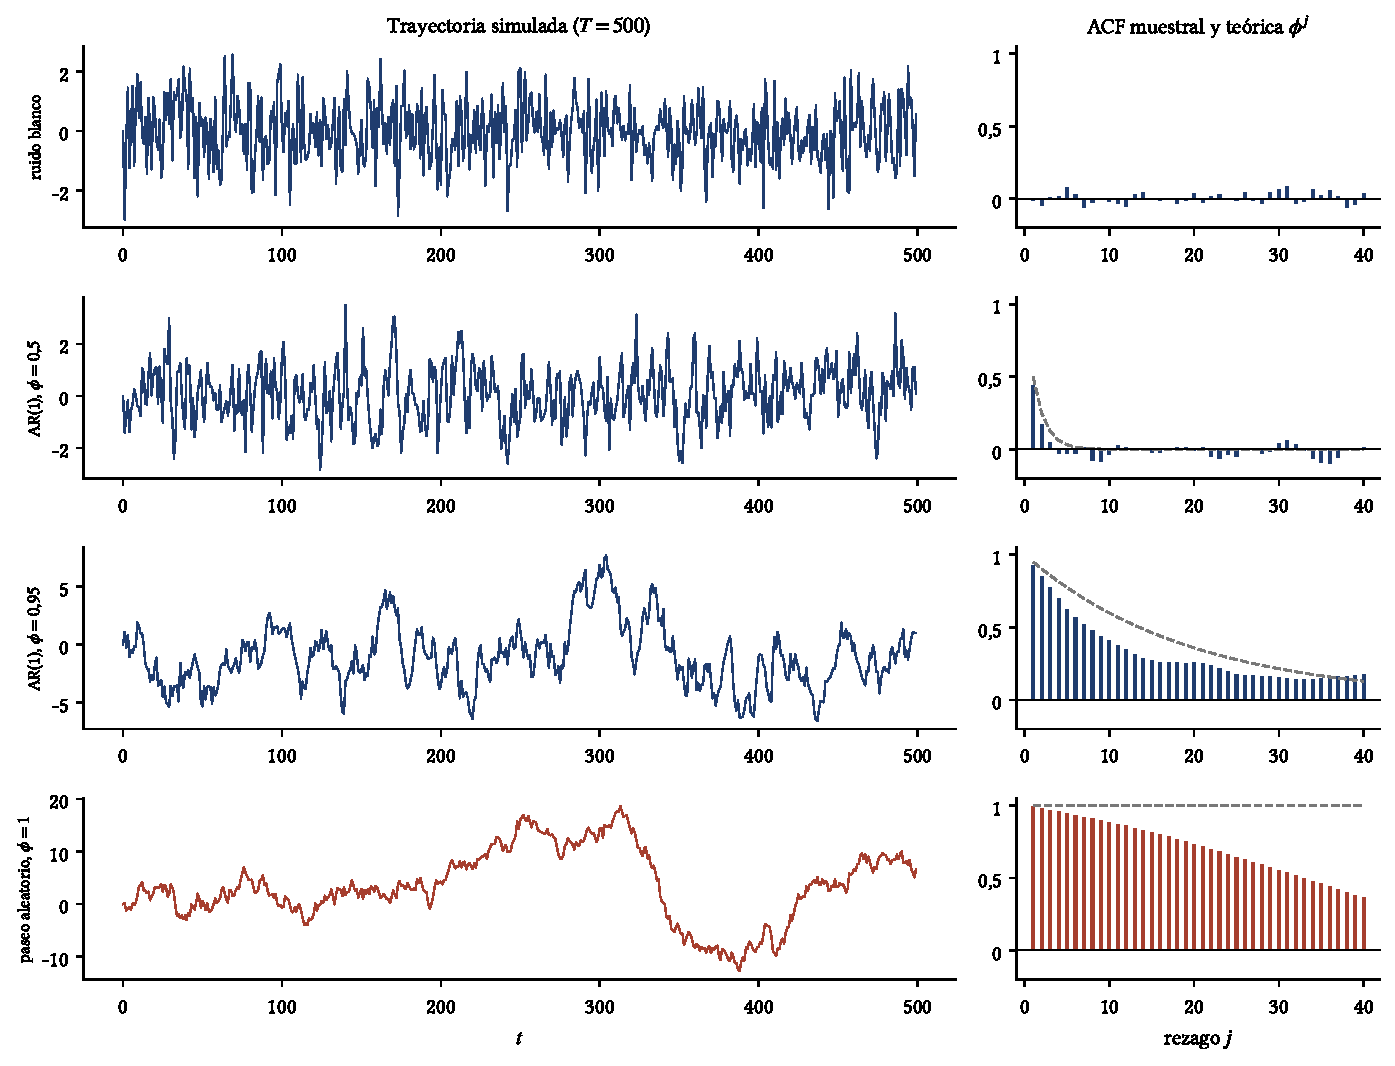
\includegraphics[width=\linewidth]{graficos/cap05_fig_procesos.pdf}
\caption{Trayectorias simuladas con los mismos choques (izquierda) y su ACF muestral (barras) frente a la
teórica $\phi^j$ (línea discontinua). Al aumentar $\phi$, la serie se aleja más tiempo de su media y la ACF
decae más despacio. El paseo aleatorio no tiene media a la que volver: deambula, y su ACF muestral queda
cerca de 1 en todos los rezagos.}
\label{fig:procesos}
\end{figure}

\begin{definicion}[Orden de integración]
Un proceso es \emph{integrado de orden $d$}, $I(d)$, si debe diferenciarse $d$ veces para volverse
estacionario. Un proceso estacionario es $I(0)$; un paseo aleatorio es $I(1)$, porque
$\Delta y_t=y_t-y_{t-1}=\varepsilon_t$ es estacionario. En finanzas, los logaritmos de los precios suelen ser
$I(1)$ y los rendimientos, $I(0)$.
\end{definicion}

\begin{proposicion}[Sobrediferenciación]\label{prop:sobrediferencia}
Si $y_t=\varepsilon_t$ es ruido blanco y se diferencia, $\Delta y_t=\varepsilon_t-\varepsilon_{t-1}$ tiene
autocorrelación de primer orden igual a $-1/2$.
\end{proposicion}

\begin{proof}
\begin{align*}
  \Var(\Delta y_t)                    &= \Var(\varepsilon_t)+\Var(\varepsilon_{t-1})\\
                                      &= 2\sigma^2,\\
  \Cov(\Delta y_t,\Delta y_{t-1})     &= \Cov(\varepsilon_t-\varepsilon_{t-1},\ \varepsilon_{t-1}-\varepsilon_{t-2})\\
                                      &= -\Var(\varepsilon_{t-1})\\
                                      &= -\sigma^2,\\
  \rho_1                              &= \frac{-\sigma^2}{2\sigma^2}\\
                                      &= -\frac12 . && \qedhere
\end{align*}
\end{proof}

Diferenciar una serie que ya era estacionaria no la ``arregla'': introduce una autocorrelación negativa
artificial. Por eso no conviene diferenciar por si acaso; hay que decidir con pruebas formales.

% ---------------------------------------------------------------------
\section{Regresión espuria}
% ---------------------------------------------------------------------

Granger y Newbold (1974) mostraron con simulaciones que, al regresar un paseo aleatorio sobre otro
\emph{independiente}, la prueba $t$ rechaza la hipótesis de pendiente nula con mucha más frecuencia que el
nivel nominal, el $R^2$ suele ser alto y el estadístico de Durbin-Watson, cercano a cero. Phillips (1986)
demostró que el estadístico $t$ no converge a ninguna distribución: crece con $\sqrt T$, de modo que con más
datos el rechazo falso es \emph{más} probable. La intuición es que ambas series tienen tendencias
estocásticas que deambulan, y en cualquier muestra finita esas tendencias parecen relacionadas.

La Figura~\ref{fig:espuria} lo confirma: en 2\,000 simulaciones por tamaño de muestra, la prueba $t$ al 5\,\%
rechaza la hipótesis verdadera de independencia el 66\,\% de las veces con $T=50$ y el 91\,\% con
$T=1\,000$. Si las mismas series se regresan en diferencias, los rechazos vuelven al 5\,\%. Una regla
práctica clásica es sospechar de cualquier regresión en niveles con $R^2$ mayor que el estadístico de
Durbin-Watson.

\begin{figure}[ht]
\centering
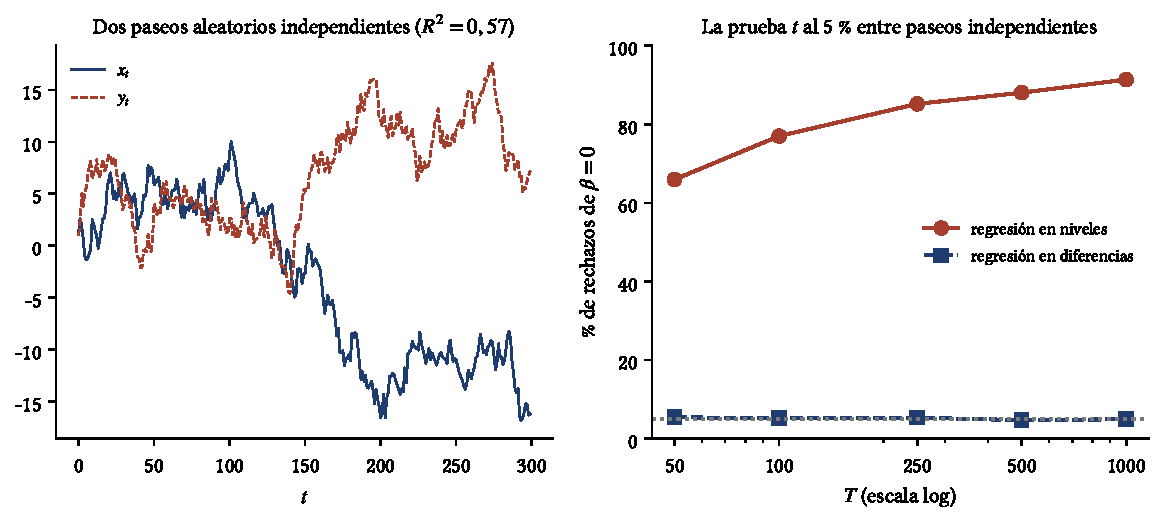
\includegraphics[width=\linewidth]{graficos/cap05_fig_espuria.pdf}
\caption{Izquierda: dos paseos aleatorios independientes, elegidos para ilustrar un caso con $R^2$ alto
($0{,}57$). Derecha: porcentaje de rechazos de $H_0:\beta=0$, que es cierta, con la prueba $t$ al 5\,\%.
En niveles, el rechazo falso aumenta con el tamaño de la muestra; en diferencias, se mantiene en el 5\,\%.}
\label{fig:espuria}
\end{figure}

% ---------------------------------------------------------------------
\section{La prueba de Dickey-Fuller}
% ---------------------------------------------------------------------

Para decidir si una serie tiene raíz unitaria, la idea natural es estimar
$y_t=\phi y_{t-1}+\varepsilon_t$ y probar $H_0:\phi=1$. Restando $y_{t-1}$ en ambos lados, la regresión
equivalente es
\[
  \Delta y_t=\gamma\,y_{t-1}+\varepsilon_t,\qquad \gamma=\phi-1,
\]
y la hipótesis nula es $H_0:\gamma=0$ (raíz unitaria) frente a $H_1:\gamma<0$ (estacionariedad). El problema
es que, bajo la hipótesis nula, el estimador no tiene la distribución habitual.

\begin{teorema}[Dickey-Fuller]\label{teo:df}
Si $y_t=y_{t-1}+\varepsilon_t$ con $y_0=0$ y $\varepsilon_t$ i.i.d. con varianza $\sigma^2$, el estimador MCO
$\hat\phi$ de la regresión sin constante cumple
\[
  T(\hat\phi-1)\ \xrightarrow{d}\ \frac{\tfrac12\bigl[W(1)^2-1\bigr]}{\int_0^1W(r)^2\,dr},
\]
donde $W$ es un movimiento browniano estándar. En particular, $\hat\phi$ converge a 1 a la velocidad $T$ (no
$\sqrt T$), y la distribución límite no es normal.
\end{teorema}

\begin{proof}
El estimador MCO es $\hat\phi=\sum_ty_{t-1}y_t/\sum_ty_{t-1}^2$. Como $y_t=y_{t-1}+\varepsilon_t$:
\begin{align*}
  \hat\phi-1 &= \frac{\sum_ty_{t-1}(y_{t-1}+\varepsilon_t)}{\sum_ty_{t-1}^2}-1\\
             &= \frac{\sum_ty_{t-1}\,\varepsilon_t}{\sum_ty_{t-1}^2}.
\end{align*}
Multiplicamos el numerador y el denominador por potencias de $T$ que los estabilizan:
\[
  T(\hat\phi-1)=\frac{T^{-1}\sum_ty_{t-1}\varepsilon_t}{T^{-2}\sum_ty_{t-1}^2}.
\]
\emph{Numerador.} Elevando al cuadrado la ecuación del paseo:
\begin{align*}
  y_t^2                    &= (y_{t-1}+\varepsilon_t)^2\\
                           &= y_{t-1}^2+2\,y_{t-1}\varepsilon_t+\varepsilon_t^2\\
  y_{t-1}\,\varepsilon_t   &= \tfrac12\bigl(y_t^2-y_{t-1}^2-\varepsilon_t^2\bigr).
\end{align*}
Sumando de $t=1$ a $T$, la suma de $y_t^2-y_{t-1}^2$ es telescópica y $y_0=0$:
\begin{align*}
  \sum_{t=1}^Ty_{t-1}\,\varepsilon_t &= \tfrac12\Bigl(y_T^2-y_0^2-\sum_{t=1}^T\varepsilon_t^2\Bigr)\\
                                     &= \tfrac12\Bigl(y_T^2-\sum_{t=1}^T\varepsilon_t^2\Bigr),\\
  \frac1{T\sigma^2}\sum_{t=1}^Ty_{t-1}\,\varepsilon_t
                                     &= \frac12\Bigl[\Bigl(\frac{y_T}{\sigma\sqrt T}\Bigr)^2-\frac{1}{T\sigma^2}\sum_{t=1}^T\varepsilon_t^2\Bigr].
\end{align*}
Por el teorema central del límite, $y_T/(\sigma\sqrt T)\to W(1)\sim N(0,1)$, y por la ley de los grandes
números, $\frac1{T\sigma^2}\sum_t\varepsilon_t^2\to1$. El numerador converge a
$\tfrac12\bigl[W(1)^2-1\bigr]$.

\emph{Denominador.} El teorema central del límite funcional (principio de invariancia de Donsker) establece
que la trayectoria reescalada $y_{\lfloor rT\rfloor}/(\sigma\sqrt T)$, $r\in[0,1]$, converge a $W(r)$. Como
$\frac{1}{T^2\sigma^2}\sum_ty_{t-1}^2$ es una suma de Riemann de $\bigl(y_{\lfloor rT\rfloor}/(\sigma\sqrt T)\bigr)^2$,
converge a $\int_0^1W(r)^2dr$. Aplicando el teorema de la aplicación continua al cociente se obtiene el
resultado (los $\sigma^2$ se cancelan).
\end{proof}

Dos consecuencias se leen directamente de la fórmula. Primera, como $W(1)^2\sim\chi^2_1$, el numerador es
negativo cuando $W(1)^2<1$, lo que ocurre con probabilidad $P(|Z|<1)=0{,}683$: $\hat\phi$ tiende a quedar
\emph{por debajo} de 1 y la distribución está sesgada a la izquierda. Segunda, el estadístico $t$ de
$\hat\gamma$ tampoco es normal; también converge a un funcional del browniano, que depende de los términos
deterministas incluidos en la regresión.

\paragraph{Términos deterministas.} En la práctica se estima una de tres regresiones: sin términos
deterministas, con constante ($\Delta y_t=\alpha+\gamma y_{t-1}+\varepsilon_t$, adecuada para series sin
tendencia, como tasas de interés o razones financieras), o con constante y tendencia lineal (adecuada para
series con tendencia, como el logaritmo de un índice bursátil). Cada caso tiene su propia distribución bajo
$H_0$. La Figura~\ref{fig:df} muestra las tres, obtenidas por simulación, y la Tabla~\ref{tab:vcdf} compara
los cuantiles simulados con los valores asintóticos de MacKinnon (2010).

\begin{figure}[ht]
\centering
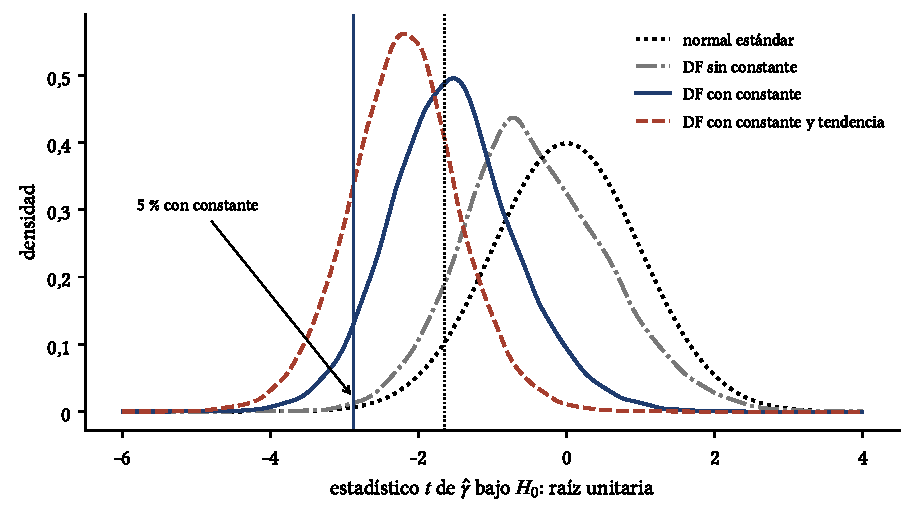
\includegraphics[width=0.82\linewidth]{graficos/cap05_fig_df.pdf}
\caption{Distribución del estadístico $t$ de Dickey-Fuller bajo la hipótesis de raíz unitaria (20\,000
simulaciones con $T=500$), frente a la normal estándar. Las tres distribuciones están desplazadas a la
izquierda, y más cuantos más términos deterministas incluye la regresión. Usar el valor crítico normal
($-1{,}645$, línea punteada) llevaría a rechazar la raíz unitaria con demasiada frecuencia.}
\label{fig:df}
\end{figure}

\begin{table}[ht]
\centering\small
\begin{tabular}{@{}lccccccc@{}}
\toprule
 & \multicolumn{3}{c}{Simulación ($T=500$)} & & \multicolumn{3}{c}{MacKinnon (asintóticos)} \\
\cmidrule{2-4}\cmidrule{6-8}
Regresión & 1\,\% & 5\,\% & 10\,\% & & 1\,\% & 5\,\% & 10\,\% \\
\midrule
Sin constante              & $-2{,}52$ & $-1{,}94$ & $-1{,}62$ & & $-2{,}57$ & $-1{,}94$ & $-1{,}62$ \\
Con constante              & $-3{,}46$ & $-2{,}88$ & $-2{,}59$ & & $-3{,}43$ & $-2{,}86$ & $-2{,}57$ \\
Con constante y tendencia  & $-3{,}97$ & $-3{,}42$ & $-3{,}14$ & & $-3{,}96$ & $-3{,}41$ & $-3{,}13$ \\
\bottomrule
\end{tabular}
\caption{Valores críticos del estadístico $t$ de Dickey-Fuller. Las simulaciones están en
\texttt{cap05\_figuras\_teoria.py}; las pequeñas diferencias con los valores asintóticos se deben al tamaño
finito de la muestra y al error de simulación.}
\label{tab:vcdf}
\end{table}

\subsection{Dickey-Fuller aumentada (ADF)}

Si los errores de la regresión están autocorrelacionados, la distribución anterior deja de valer. La
solución de Said y Dickey (1984) es añadir rezagos de la variable dependiente:
\[
  \Delta y_t=\alpha+\beta t+\gamma\,y_{t-1}+\sum_{j=1}^{p}\delta_j\,\Delta y_{t-j}+\varepsilon_t,
\]
con los términos deterministas que correspondan. El estadístico es el $t$ de $\hat\gamma$ y se compara con
los mismos valores críticos. El número de rezagos $p$ se elige con un criterio de información (en este libro,
el AIC) en una muestra común, partiendo de un máximo $p_{\max}=\lfloor12(T/100)^{1/4}\rfloor$ (Schwert, 1989).

\subsection{Phillips-Perron}

Phillips y Perron (1988) proponen otra solución: estimar la regresión de Dickey-Fuller sin rezagos y
corregir el estadístico $t$ con una estimación no paramétrica de la varianza de largo plazo, del mismo tipo
que el estimador de Newey-West del Capítulo~\ref{cap:robustos}. Tiene la misma distribución límite que la
prueba ADF y es robusta a heterocedasticidad de forma general, pero en muestras finitas suele tener peor
tamaño cuando los errores tienen autocorrelación negativa fuerte.

% ---------------------------------------------------------------------
\section{La prueba KPSS: estacionariedad como hipótesis nula}
% ---------------------------------------------------------------------

Las pruebas ADF y PP tienen poca potencia frente a alternativas muy persistentes: con $\phi=0{,}98$ es muy
difícil distinguir un AR(1) de un paseo aleatorio en una muestra moderada. Como la hipótesis nula es la
raíz unitaria, ``no rechazar'' es la respuesta por defecto cuando los datos no son concluyentes. Kwiatkowski,
Phillips, Schmidt y Shin (1992) invierten las hipótesis.

\begin{definicion}[Prueba KPSS]
Sea $\hat e_t$ el residuo de regresar $y_t$ sobre una constante (o sobre una constante y una tendencia), y
$S_t=\sum_{s=1}^t\hat e_s$ su suma parcial. El estadístico es
\[
  \eta=\frac{1}{T^2\,\hat\sigma^2_{\mathrm{LP}}}\sum_{t=1}^TS_t^2,
\]
donde $\hat\sigma^2_{\mathrm{LP}}$ es la varianza de largo plazo de $\hat e_t$, estimada con el núcleo de
Bartlett y $l$ rezagos. La hipótesis nula es la estacionariedad y se rechaza para valores \emph{grandes} de
$\eta$. Los valores críticos al 10\,\%, 5\,\% y 1\,\% son $0{,}347$; $0{,}463$ y $0{,}739$ con constante, y
$0{,}119$; $0{,}146$ y $0{,}216$ con tendencia.
\end{definicion}

La intuición está en la Figura~\ref{fig:kpss}. Si la serie es estacionaria, sus desviaciones respecto de la
media se compensan y las sumas parciales oscilan cerca de cero. Si tiene raíz unitaria, pasa largos períodos
por encima o por debajo de su media muestral, y las sumas parciales se alejan mucho: $\eta$ es grande.

\begin{figure}[ht]
\centering
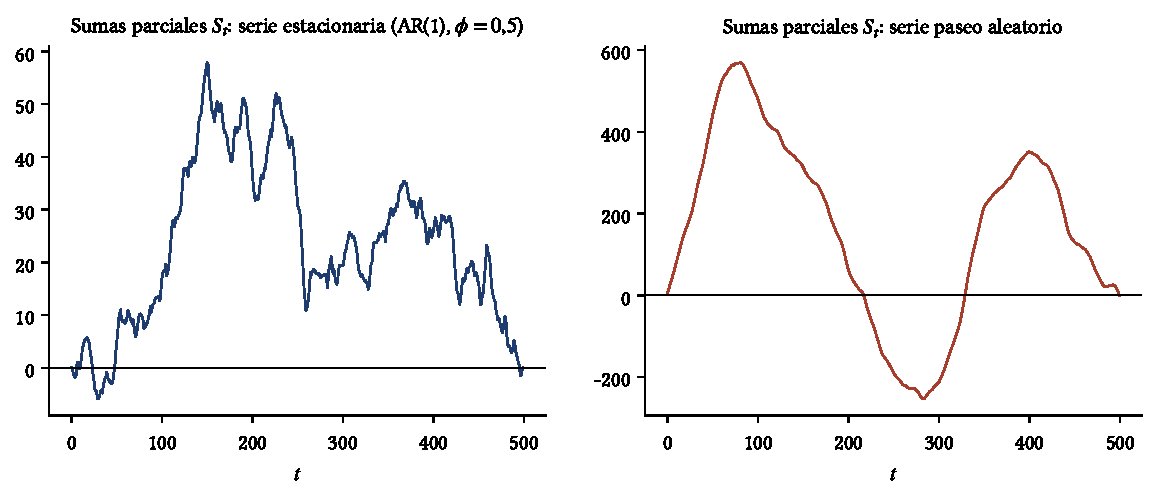
\includegraphics[width=\linewidth]{graficos/cap05_fig_kpss.pdf}
\caption{Sumas parciales de las desviaciones respecto de la media para una serie estacionaria (izquierda) y
para un paseo aleatorio (derecha). Observe la escala: en el paseo aleatorio son decenas de veces mayores.}
\label{fig:kpss}
\end{figure}

\paragraph{Análisis confirmatorio.} Usar juntas las pruebas ADF y KPSS da cuatro resultados posibles:
\begin{center}\small
\begin{tabular}{@{}lll@{}}
\toprule
ADF (nula: raíz unitaria) & KPSS (nula: estacionaria) & Conclusión \\
\midrule
Rechaza       & No rechaza & Estacionaria \\
No rechaza    & Rechaza    & Raíz unitaria \\
No rechaza    & No rechaza & Datos poco informativos \\
Rechaza       & Rechaza    & Ni una cosa ni la otra: memoria larga o quiebres \\
\bottomrule
\end{tabular}
\end{center}

% ---------------------------------------------------------------------
\section{Quiebres estructurales y raíces unitarias}
% ---------------------------------------------------------------------

Perron (1989) mostró que una serie estacionaria con un cambio de nivel puede parecer un paseo aleatorio: el
salto es un choque ``permanente'', y la prueba ADF lo interpreta como evidencia de raíz unitaria. La
Figura~\ref{fig:perron} muestra un ejemplo: un AR(1) con $\phi=0{,}9$ y un salto de 10 unidades a mitad de la
muestra. En 2\,000 simulaciones, la prueba ADF rechaza la raíz unitaria solo el 0,1\,\% de las veces; si se
elimina el salto, la rechaza el 99,8\,\%.

\begin{figure}[ht]
\centering
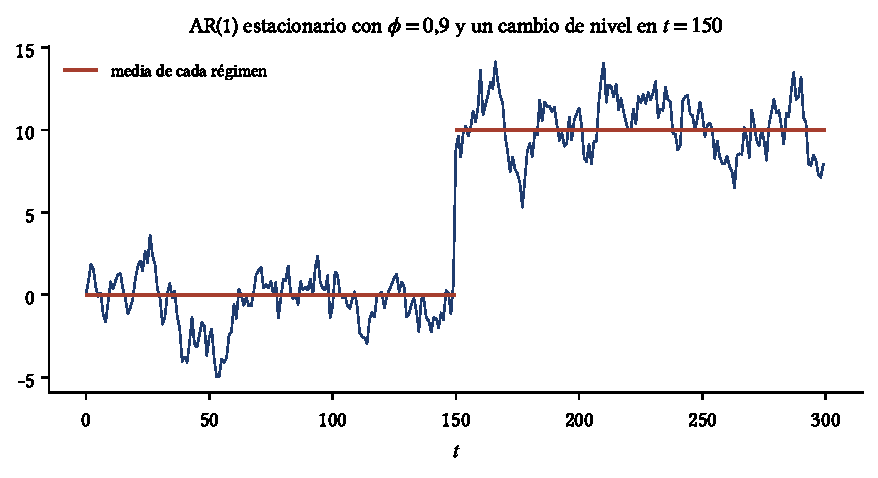
\includegraphics[width=0.82\linewidth]{graficos/cap05_fig_perron.pdf}
\caption{Una serie estacionaria alrededor de una media que cambia una sola vez. Dentro de cada régimen la
serie vuelve rápidamente a su media; vista en conjunto, parece haberse desplazado para siempre, como un
paseo aleatorio.}
\label{fig:perron}
\end{figure}

\begin{definicion}[Prueba de Zivot-Andrews]
Para cada fecha candidata $T_B$ entre el 15\,\% y el 85\,\% de la muestra se estima
\[
  \Delta y_t=\alpha+\theta\,DU_t(T_B)+\beta t+\gamma\,y_{t-1}+\sum_{j=1}^p\delta_j\,\Delta y_{t-j}+\varepsilon_t,
  \qquad DU_t(T_B)=\mathbb 1\{t\ge T_B\},
\]
y se toma el mínimo de los estadísticos $t$ de $\hat\gamma$. La hipótesis nula es la raíz unitaria sin
quiebre; la alternativa, estacionariedad con un cambio de nivel en una fecha desconocida. Los valores
críticos son más negativos que los de ADF: $-5{,}34$, $-4{,}80$ y $-4{,}58$ al 1\,\%, 5\,\% y 10\,\%
(Zivot y Andrews, 1992).
\end{definicion}

% ---------------------------------------------------------------------
\section{Ejercicios resueltos}
% ---------------------------------------------------------------------

Las pruebas ADF y KPSS están programadas desde las fórmulas del texto en los archivos
\texttt{cap05\_funciones} de las carpetas de código de R y de Python, que se muestran en el primer
ejercicio. En Python comprobamos cada resultado con el paquete \texttt{arch}.

\begin{ejresuelto}{¿Tiene raíz unitaria el precio del petróleo?}\label{ej:brentur}
\enunciado Con el Brent diario: (a) aplique las pruebas ADF y KPSS al logaritmo del precio, con constante y
con constante y tendencia; (b) aplíquelas al rendimiento logarítmico; (c) concluya el orden de integración.

\solucion
\paso{Paso 1. Logaritmo del precio.} El AIC elige $p=29$ rezagos. Con constante:
\begin{align*}
  t_{\mathrm{ADF}} &= -1{,}912\\
                   &> -2{,}86 \quad\text{(valor crítico al 5\,\%)},\\
  \eta_{\mathrm{KPSS}} &= 16{,}749\\
                       &> 0{,}463 \quad\text{(valor crítico al 5\,\%)}.
\end{align*}
La prueba ADF no rechaza la raíz unitaria y la KPSS rechaza la estacionariedad con mucha holgura. Con
tendencia, $t_{\mathrm{ADF}}=-3{,}179>-3{,}41$ y $\eta=2{,}622>0{,}146$: la conclusión no cambia.

\paso{Paso 2. Rendimiento.} Con $p=28$ rezagos:
\begin{align*}
  t_{\mathrm{ADF}}     &= -17{,}108 < -2{,}86,\\
  \eta_{\mathrm{KPSS}} &= 0{,}027 < 0{,}463 .
\end{align*}
ADF rechaza la raíz unitaria y KPSS no rechaza la estacionariedad.

\paso{Paso 3. Conclusión.} El logaritmo del precio del Brent es $I(1)$ y su rendimiento es $I(0)$. Los
choques al precio del petróleo son permanentes: la caída de 2020 no fue ``revertida'' por una fuerza que
devolviera el precio a un nivel normal; el precio partió desde su nuevo nivel.

\codigoweb{cap05_ej01}
\salidaR{cap05_ej01_R.txt}
\lectura{cap05_ej01}

\RvsPy Las funciones están escritas de forma paralela en los dos lenguajes, y la única diferencia de fondo
es la indexación: en R la primera fila de la regresión es \texttt{p + 1} y en Python \texttt{p}. La salida
de Python incluye la comprobación con \texttt{arch}: con el mismo número de rezagos, los estadísticos
coinciden en todas las cifras, y \texttt{arch} añade los $p$-valores de MacKinnon. En R el paquete
\texttt{urca} ofrece las mismas pruebas.

\begin{figure}[ht]
\centering
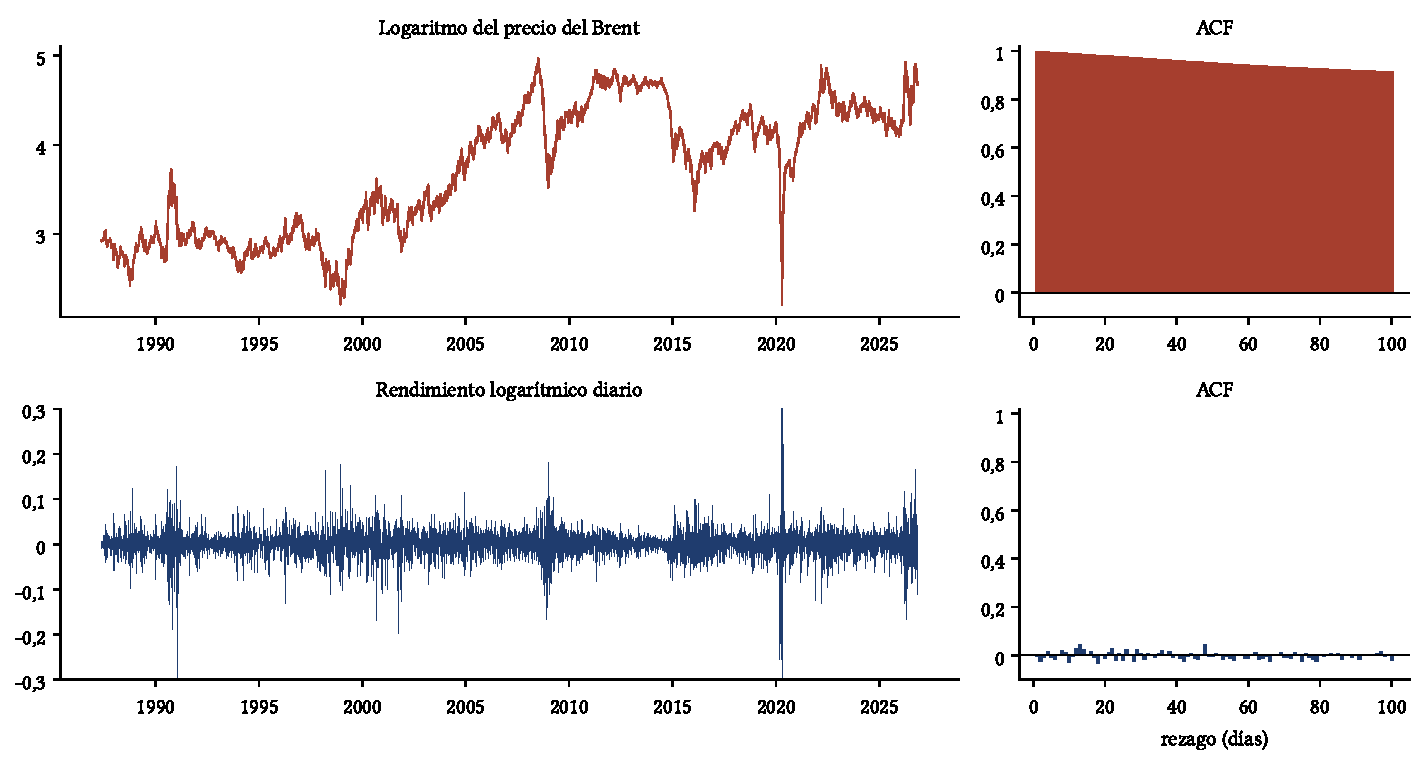
\includegraphics[width=\linewidth]{graficos/cap05_fig_brent.pdf}
\caption{Arriba: el logaritmo del precio del Brent deambula sin una media a la que volver, y su ACF casi no
decae. Abajo: el rendimiento oscila alrededor de cero, con la ACF de un ruido blanco.}
\label{fig:brentur}
\end{figure}

\begin{conclusion}
El precio del petróleo tiene raíz unitaria y su rendimiento es estacionario, como predice la hipótesis de
mercados eficientes. Los modelos de los capítulos siguientes se estiman sobre rendimientos.
\end{conclusion}
\end{ejresuelto}

\begin{ejresuelto}{El VIX: estacionario, pero persistente}\label{ej:vixur}
\enunciado Con el logaritmo del VIX diario: (a) aplique las pruebas ADF y KPSS con constante; (b) estime un
AR(1) y calcule su media de largo plazo y la vida media de un choque; (c) interprete el conjunto de
resultados.

\solucion
\paso{Paso 1. Pruebas.}
\begin{align*}
  t_{\mathrm{ADF}}     &= -6{,}539 < -2{,}86,\\
  \eta_{\mathrm{KPSS}} &= 0{,}568 > 0{,}463 .
\end{align*}
ADF rechaza con claridad la raíz unitaria. KPSS rechaza la estacionariedad al 5\,\%, aunque no al 1\,\%
(valor crítico $0{,}739$). Es el cuarto caso del análisis confirmatorio: ambas rechazan.

\paso{Paso 2. AR(1).} La estimación MCO da $\hat c=0{,}05824$ y $\hat\phi=0{,}97994$. Entonces
\begin{align*}
  \hat\mu &= \frac{\hat c}{1-\hat\phi}\\
          &= \frac{0{,}05824}{1-0{,}97994}\\
          &= 2{,}903,\\
  e^{\hat\mu} &= 18{,}23 .
\end{align*}
El VIX tiende a volver a un nivel de 18,2 puntos. La vida media de un choque es
\begin{align*}
  h^* &= \frac{\ln0{,}5}{\ln\hat\phi}\\
      &= \frac{-0{,}69315}{\ln0{,}97994}\\
      &= \frac{-0{,}69315}{-0{,}02026}\\
      &= 34{,}2 \text{ días}.
\end{align*}

\paso{Paso 3. Interpretación.} El VIX vuelve a su media: un salto del miedo del mercado se reduce a la mitad
en unas siete semanas de negociación. La Figura~\ref{fig:vixur} muestra, sin embargo, que la ACF decae mucho
más despacio que $\hat\phi^j$: a 250 días es $0{,}35$, cuando el AR(1) predice $0{,}006$. Esa es la huella de la \emph{memoria
larga}, un comportamiento intermedio entre $I(0)$ e $I(1)$ que explica por qué las dos pruebas rechazan a la
vez: la serie es demasiado persistente para KPSS y demasiado reversible para ADF.

\codigoweb{cap05_ej02}
\salidaR{cap05_ej02_R.txt}
\lectura{cap05_ej02}

\RvsPy En R, \texttt{lm(y[-1] \textasciitilde{} y[-T])} regresa cada valor sobre el anterior quitando el
primero y el último elemento; en Python se obtiene lo mismo con \texttt{y[1:]} y \texttt{y[:-1]}.

\begin{figure}[ht]
\centering
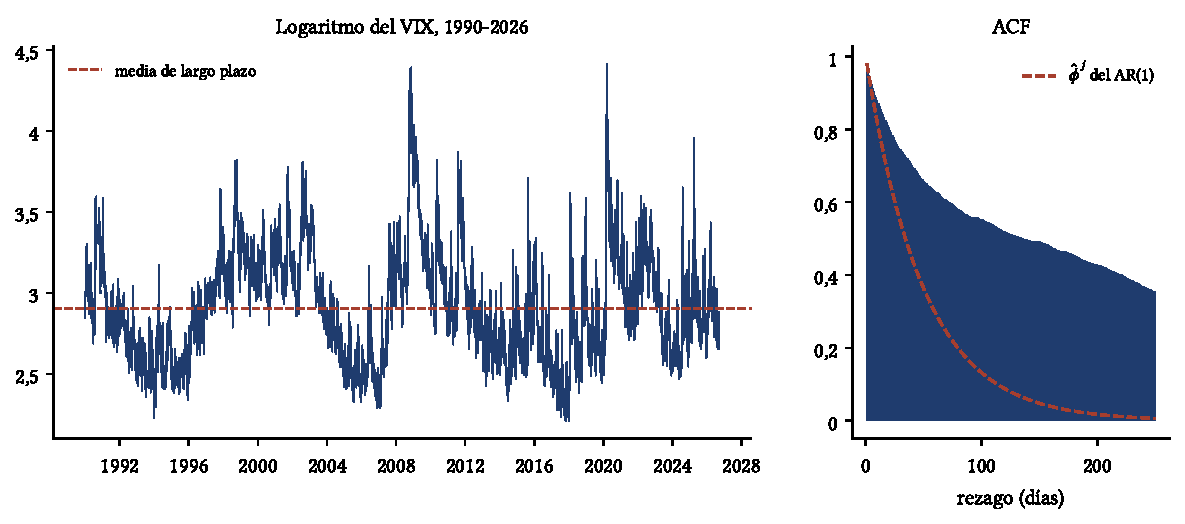
\includegraphics[width=\linewidth]{graficos/cap05_fig_vix.pdf}
\caption{Izquierda: el logaritmo del VIX vuelve siempre a su media de largo plazo, aunque con episodios largos
lejos de ella (2008, 2020). Derecha: su ACF decae mucho más despacio que la de un AR(1) con el mismo
$\hat\phi$.}
\label{fig:vixur}
\end{figure}

\begin{conclusion}
El VIX es estacionario en el sentido económico relevante: vuelve a su media, con una vida media de unos 34
días hábiles. Pero su dependencia de largo plazo es más fuerte que la de un AR(1), un rasgo que comparten
la volatilidad y el volumen de casi todos los activos (Capítulo~\ref{cap:hechos}).
\end{conclusion}
\end{ejresuelto}

\begin{ejresuelto}{La tasa de interés de largo plazo: la prueba ADF paso a paso}\label{ej:tasaur}
\enunciado Con el rendimiento mensual del bono del Tesoro de EE.\,UU. a 10 años (1871--2023): (a) elija el
número de rezagos por AIC; (b) estime la regresión ADF con constante y calcule el estadístico; (c) repita en
diferencias y con la prueba KPSS.

\solucion
\paso{Paso 1. Rezagos.} Con $T=1\,830$ meses, el máximo es
\begin{align*}
  p_{\max} &= \Bigl\lfloor 12\Bigl(\frac{1\,830}{100}\Bigr)^{1/4}\Bigr\rfloor\\
           &= \lfloor 12\times2{,}068\rfloor\\
           &= \lfloor 24{,}8\rfloor\\
           &= 24,
\end{align*}
y el AIC elige $p=22$.

\paso{Paso 2. Estadístico.} En la regresión ADF, $\hat\gamma=-0{,}00288$ con error estándar $0{,}00169$:
\begin{align*}
  t_{\mathrm{ADF}} &= \frac{\hat\gamma}{\operatorname{ee}(\hat\gamma)}\\
                   &= \frac{-0{,}00288}{0{,}00169}\\
                   &= -1{,}70,
\end{align*}
($-1{,}701$ con todos los decimales), mayor que $-2{,}57$, el valor crítico al 10\,\%: no se rechaza la raíz
unitaria. El coeficiente implica $\hat\phi=1+\hat\gamma=0{,}99712$, una persistencia altísima.

\paso{Paso 3. Diferencias y KPSS.} En diferencias, $t_{\mathrm{ADF}}=-10{,}373$: se rechaza la raíz unitaria.
KPSS da $\eta=1{,}164$ en niveles (rechaza la estacionariedad) y $\eta=0{,}075$ en diferencias (no la
rechaza). La tasa de interés se comporta como $I(1)$.

\paso{Paso 4. Interpretación.} Una tasa de interés no puede ser un paseo aleatorio en sentido estricto:
estaría acotada por debajo y la economía no permite que crezca sin límite. Lo que dice la prueba es que su
reversión a la media, si existe, es tan lenta que en 150 años de datos no se distingue de una raíz unitaria.
A efectos prácticos de modelación (Capítulos~10 y~11) se trata como $I(1)$.

\codigoweb{cap05_ej03}
\salidaR{cap05_ej03_R.txt}
\lectura{cap05_ej03}

\RvsPy Al leer el CSV, R convierte el nombre de columna \texttt{Long Interest Rate} en
\texttt{Long.Interest.Rate} (reemplaza los espacios por puntos); \texttt{pandas} conserva el nombre original.

\begin{figure}[ht]
\centering
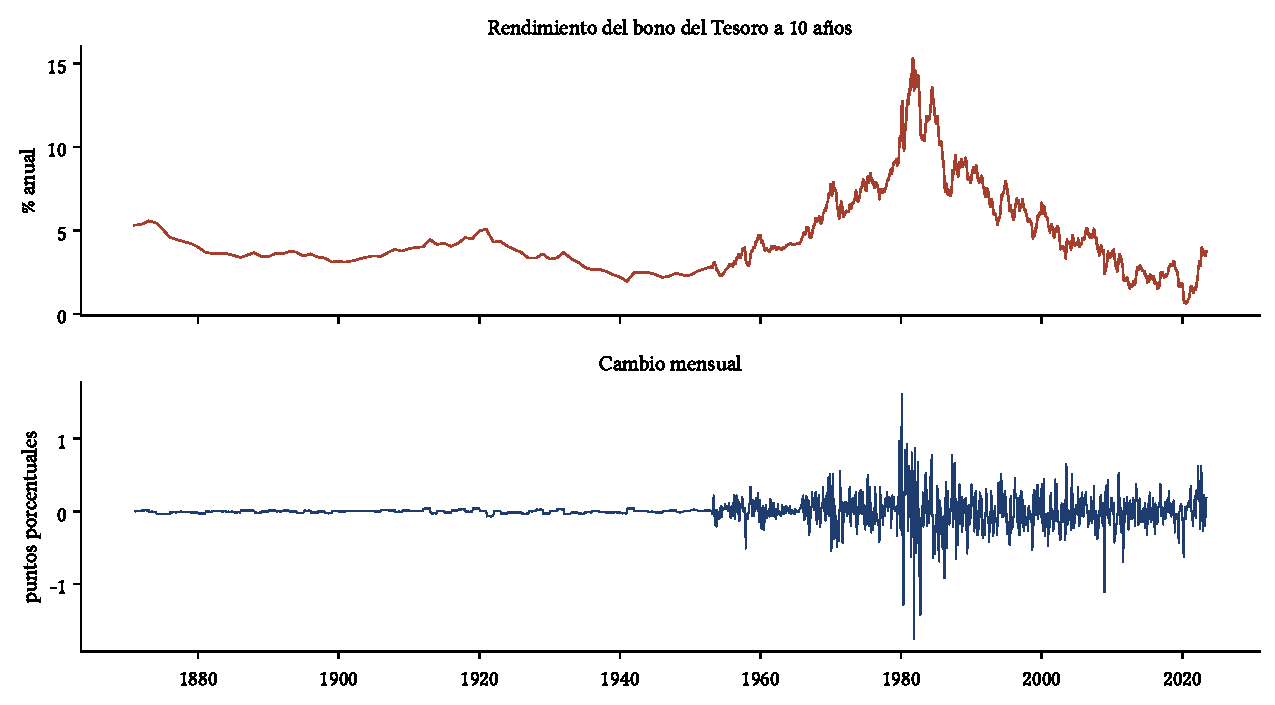
\includegraphics[width=0.9\linewidth]{graficos/cap05_fig_tasa.pdf}
\caption{Arriba: la tasa a 10 años pasa décadas lejos de cualquier promedio (el mínimo de los años cuarenta,
el máximo de 1981, los mínimos de 2020). Abajo: sus cambios mensuales oscilan alrededor de cero, con
volatilidad mucho mayor a partir de los años setenta.}
\label{fig:tasaur}
\end{figure}

\begin{conclusion}
La tasa de interés de largo plazo es $I(1)$ para fines estadísticos. Esto tiene consecuencias inmediatas:
una regresión de otra variable en niveles sobre la tasa de interés corre el riesgo de ser espuria, salvo que
exista cointegración (Capítulo~11).
\end{conclusion}
\end{ejresuelto}

\begin{ejresuelto}{Oro y acciones: una regresión espuria con datos reales}\label{ej:oroespuria}
\enunciado Con datos mensuales de 1975 a 2026: (a) verifique que los logaritmos del precio del oro y del
S\&P 500 son $I(1)$; (b) regrese el primero sobre el segundo en niveles y reporte $\hat b$, $t$, $R^2$ y el
estadístico de Durbin-Watson; (c) haga la misma regresión en diferencias; (d) interprete.

\solucion
\paso{Paso 1. Orden de integración.} En niveles, $t_{\mathrm{ADF}}=-0{,}861$ (oro) y $-0{,}091$ (S\&P 500),
lejos de $-2{,}86$; en diferencias, $-7{,}391$ y $-9{,}919$. Las dos series son $I(1)$.

\paso{Paso 2. Niveles.} Con $T=621$ meses:
\begin{align*}
  \hat b &= 0{,}530, & t &= 32{,}85, & R^2 &= 0{,}636, & DW &= 0{,}0096 .
\end{align*}
Según esta regresión, un aumento de 1\,\% en el S\&P 500 se asocia con un aumento de 0,53\,\% en el oro, con
un estadístico $t$ enorme. Pero la regla de Granger y Newbold se cumple con creces:
\begin{align*}
  R^2 = 0{,}636 &> DW = 0{,}0096 .
\end{align*}
Además, el ADF de los residuos es $-2{,}100$. Con los valores críticos de Dickey-Fuller ($-1{,}94$ sin
constante) parecería rechazar la raíz unitaria, pero esos valores no son válidos para residuos estimados: MCO
elige la recta que hace los residuos lo más estacionarios posible. Los valores críticos correctos (de
Engle-Granger, Capítulo~11) son de alrededor de $-3{,}34$ al 5\,\% para dos variables, y $-2{,}100$ no los
alcanza: no hay evidencia de que las series compartan una tendencia común.

\paso{Paso 3. Diferencias.}
\begin{align*}
  \hat b &= 0{,}015, & t &= 0{,}30, & R^2 &= 0{,}00015 .
\end{align*}
Los rendimientos mensuales del oro y del S\&P 500 no están relacionados.

\codigoweb{cap05_ej04}
\salidaR{cap05_ej04_R.txt}
\lectura{cap05_ej04}

\RvsPy Unimos las dos bases por mes con \texttt{merge} en R y \texttt{merge} en \texttt{pandas}. La base de
Shiller tiene fechas completas (\texttt{1975-01-01}) y la del oro solo año y mes (\texttt{1975-01}), así que
primero extraemos los siete primeros caracteres. Si se unieran por la fecha completa, la intersección
quedaría vacía sin ningún mensaje de error.

\begin{figure}[ht]
\centering
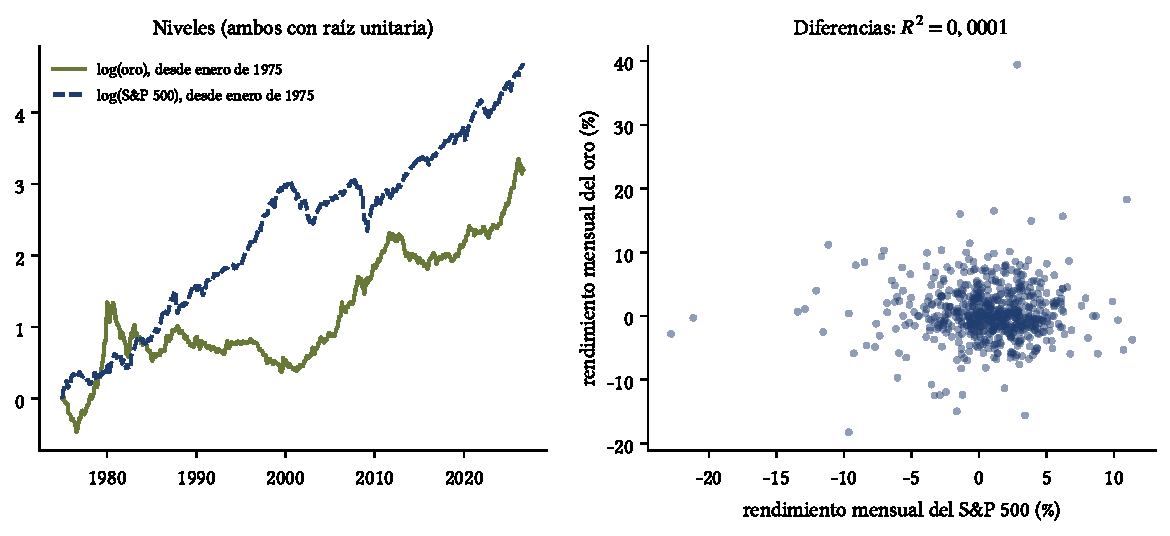
\includegraphics[width=\linewidth]{graficos/cap05_fig_oro.pdf}
\caption{Izquierda: los dos precios crecieron en el largo plazo, y eso basta para que una regresión en niveles
encuentre una relación ``muy significativa''. Derecha: los rendimientos mensuales no muestran ninguna
relación.}
\label{fig:oro}
\end{figure}

\begin{conclusion}
La relación en niveles entre el oro y las acciones es espuria: refleja que ambas series tienen tendencias
estocásticas, no que una explique a la otra. Antes de interpretar una regresión entre series financieras en
niveles hay que verificar su orden de integración y, si son $I(1)$, si están cointegradas.
\end{conclusion}
\end{ejresuelto}

\begin{ejresuelto}{¿Raíz unitaria o quiebre? La razón dividendo/precio}\label{ej:zaur}
\enunciado Con el logaritmo de la razón dividendo/precio del S\&P 500 (1871--2023): (a) aplique la prueba ADF
con tendencia; (b) aplique la prueba de Zivot-Andrews con cambio de nivel, programada a mano, y compárela con
el paquete \texttt{arch}; (c) interprete la fecha del quiebre.

\solucion
\paso{Paso 1. ADF.} Con $p=21$ rezagos, $t_{\mathrm{ADF}}=-2{,}915>-3{,}41$: no se rechaza la raíz unitaria.
Esto es incómodo para la teoría: si la razón dividendo/precio tuviera raíz unitaria, precios y dividendos se
alejarían sin límite, y la regresión predictiva del Ejercicio~\ref{ej:dprediccion} sería espuria.

\paso{Paso 2. Zivot-Andrews.} Recorriendo las 1\,282 fechas candidatas entre el 15\,\% y el 85\,\% de la
muestra, el mínimo del estadístico es
\begin{align*}
  t_{\mathrm{ZA}} &= -4{,}354 \quad\text{(noviembre de 1990)}\\
                  &> -4{,}80 \quad\text{(valor crítico al 5\,\%)}.
\end{align*}
El paquete \texttt{arch} da el mismo valor, con $p=0{,}169$. Ni siquiera permitiendo un cambio de nivel se
rechaza la raíz unitaria.

\paso{Paso 3. Interpretación.} La fecha elegida coincide con un hecho documentado: desde los años noventa las
empresas estadounidenses sustituyeron dividendos por recompras de acciones, y la razón dividendo/precio cayó
a un nivel permanentemente más bajo (Lettau y Van Nieuwerburgh, 2008). Pero el estadístico no alcanza el
valor crítico: con un solo quiebre de nivel, la serie sigue pareciendo $I(1)$. Puede deberse a que hay más de
un quiebre, a que la reversión es muy lenta o a la baja potencia de las pruebas. En el Capítulo~17 volveremos
a esta serie con modelos de cambio de régimen.

\codigoweb{cap05_ej05}
\salidaR{cap05_ej05_R.txt}
\lectura{cap05_ej05}

\RvsPy Lo más delicado es definir la variable indicadora: la fila $k$ de la regresión explica $\Delta y$ en el
período $k+1$, así que $DU=1$ cuando $k+1\ge T_B$. Con esa convención, las versiones de R (índices desde 1) y
de Python (desde 0) recorren las mismas fechas y coinciden con \texttt{arch}.

\begin{figure}[ht]
\centering
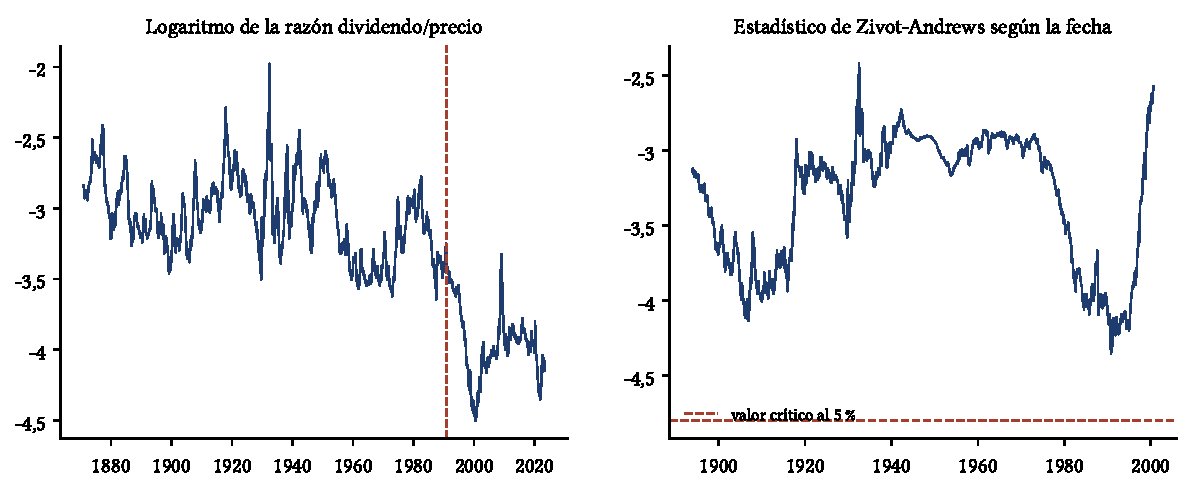
\includegraphics[width=\linewidth]{graficos/cap05_fig_za.pdf}
\caption{Izquierda: la razón dividendo/precio, con la fecha de quiebre que elige la prueba (noviembre de
1990). Derecha: el estadístico de Zivot-Andrews para cada fecha candidata; nunca baja del valor crítico al
5\,\%.}
\label{fig:za}
\end{figure}

\begin{conclusion}
La razón dividendo/precio es extremadamente persistente, con un probable cambio de nivel en los años noventa,
pero las pruebas no permiten rechazar que tenga raíz unitaria. Este es un ejemplo de lo difícil que es, con
datos financieros, separar raíces unitarias, quiebres y reversión lenta.
\end{conclusion}
\end{ejresuelto}

% ---------------------------------------------------------------------
\section{Ejercicios propuestos}
% ---------------------------------------------------------------------

\begin{enumerate}[label=\textbf{\thechapter.\arabic*},leftmargin=*,itemsep=6pt]
  \item Demuestre que en un AR(1) estacionario la PACF es $\phi_{11}=\phi$ y $\phi_{jj}=0$ para $j\ge2$.
  \textit{Pista: escriba la regresión poblacional de $y_t$ sobre $y_{t-1}$ y $y_{t-2}$ y use la
  Proposición~\ref{prop:ar1}.}

  \item Calcule la vida media de un choque si $\phi=0{,}5$; $0{,}9$; $0{,}99$ y $0{,}999$, con datos diarios.
  \textit{Respuesta: 1,0; 6,6; 69,0 y 692,8 días.}

  \item Para un paseo aleatorio con deriva, $y_t=c+y_{t-1}+\varepsilon_t$, demuestre que
  $\E[y_t]=y_0+c\,t$. ¿Por qué la prueba ADF con solo constante es inadecuada para esta serie?

  \item Demuestre que $P\bigl(T(\hat\phi-1)<0\bigr)\to P(\chi^2_1<1)=0{,}683$ bajo la hipótesis de raíz
  unitaria, usando el Teorema~\ref{teo:df}. ¿Qué implica para el sesgo de $\hat\phi$?

  \item \emph{(Simulación.)} Modifique \texttt{cap05\_figuras\_teoria.py} para estimar la potencia de la
  prueba ADF con constante (proporción de rechazos) cuando la serie es un AR(1) con $\phi=0{,}95$, para
  $T=100$, $250$ y $1\,000$. ¿Cuántos años de datos mensuales se necesitan para distinguir $\phi=0{,}95$ de
  una raíz unitaria con una potencia del 80\,\%?

  \item \emph{(Con datos.)} Aplique las pruebas ADF y KPSS al logaritmo del S\&P 500 de Shiller, con constante
  y tendencia. ¿Es $I(1)$? ¿Qué pasa con la inflación mensual calculada a partir del IPC de la misma base?

  \item \emph{(Con datos del BCRP.)} Aplique las pruebas ADF, KPSS y Zivot-Andrews al tipo de cambio
  interbancario soles por dólar desde 2000. ¿Detecta la prueba de Zivot-Andrews un quiebre? ¿En qué fecha?

  \item \emph{(Con datos del BCRP.)} Aplique las pruebas a la tasa de referencia de la política monetaria del
  BCRP. Discuta por qué una serie que el banco central fija por decisión administrativa puede comportarse
  estadísticamente como $I(1)$.
\end{enumerate}

% ---------------------------------------------------------------------
\section{Resumen de fórmulas}
% ---------------------------------------------------------------------

\begin{table}[H]
\centering\small
\begin{tabular}{@{}ll@{}}
\toprule
Concepto & Fórmula \\
\midrule
AR(1) estacionario & $\mu=c/(1-\phi)$;\quad $\gamma_0=\sigma^2/(1-\phi^2)$;\quad $\rho_j=\phi^j$ \\
Vida media & $h^*=\ln0{,}5/\ln\phi$ \\
Paseo aleatorio & $\Var(y_t)=t\sigma^2$;\quad $\operatorname{Corr}(y_t,y_s)=\sqrt{s/t}$ \\
Sobrediferenciación & $\rho_1(\Delta\varepsilon_t)=-1/2$ \\
Dickey-Fuller & $T(\hat\phi-1)\to\frac12[W(1)^2-1]/\int_0^1W^2$ \\
ADF & $\Delta y_t=\alpha+\beta t+\gamma y_{t-1}+\sum_{j=1}^p\delta_j\Delta y_{t-j}+\varepsilon_t$ \\
Valores críticos ADF al 5\,\% & $-1{,}94$ (sin constante);\quad $-2{,}86$ (constante);\quad $-3{,}41$ (tendencia) \\
KPSS & $\eta=\sum_tS_t^2/(T^2\hat\sigma^2_{\mathrm{LP}})$;\quad 5\,\%: $0{,}463$ (constante), $0{,}146$ (tendencia) \\
Zivot-Andrews (cambio de nivel) & 5\,\%: $-4{,}80$ \\
\bottomrule
\end{tabular}
\caption{Fórmulas principales del Capítulo 5.}
\end{table}

\section*{Referencias}
\begin{itemize}[leftmargin=*]
  \item Dickey, D. A. y Fuller, W. A. (1979). Distribution of the estimators for autoregressive time series
        with a unit root. \emph{Journal of the American Statistical Association}, 74(366), 427--431.
  \item Granger, C. W. J. y Newbold, P. (1974). Spurious regressions in econometrics. \emph{Journal of
        Econometrics}, 2(2), 111--120.
  \item Hamilton, J. D. (1994). \emph{Time Series Analysis}. Princeton University Press. Capítulos 3 y 17.
  \item Kwiatkowski, D., Phillips, P. C. B., Schmidt, P. y Shin, Y. (1992). Testing the null hypothesis of
        stationarity against the alternative of a unit root. \emph{Journal of Econometrics}, 54(1--3),
        159--178.
  \item Lettau, M. y Van Nieuwerburgh, S. (2008). Reconciling the return predictability evidence.
        \emph{The Review of Financial Studies}, 21(4), 1607--1652.
  \item MacKinnon, J. G. (2010). Critical values for cointegration tests. Queen's Economics Department
        Working Paper No. 1227.
  \item Perron, P. (1989). The great crash, the oil price shock, and the unit root hypothesis.
        \emph{Econometrica}, 57(6), 1361--1401.
  \item Phillips, P. C. B. (1986). Understanding spurious regressions in econometrics. \emph{Journal of
        Econometrics}, 33(3), 311--340.
  \item Phillips, P. C. B. y Perron, P. (1988). Testing for a unit root in time series regression.
        \emph{Biometrika}, 75(2), 335--346.
  \item Said, S. E. y Dickey, D. A. (1984). Testing for unit roots in autoregressive-moving average models of
        unknown order. \emph{Biometrika}, 71(3), 599--607.
  \item Schwert, G. W. (1989). Tests for unit roots: a Monte Carlo investigation. \emph{Journal of Business
        \& Economic Statistics}, 7(2), 147--159.
  \item Zivot, E. y Andrews, D. W. K. (1992). Further evidence on the great crash, the oil-price shock, and the
        unit-root hypothesis. \emph{Journal of Business \& Economic Statistics}, 10(3), 251--270.
\end{itemize}

% =====================================================================
%  Capítulo 6. Modelos ARMA
% =====================================================================
\chapter[Modelos ARMA]{Modelos ARMA: identificación, estimación, diagnóstico y pronóstico}\label{cap:arma}

\section*{Objetivos de aprendizaje}
Al terminar este capítulo, el lector podrá:
\begin{enumerate}[label=\arabic*.,leftmargin=*]
  \item Derivar los momentos y la función de autocorrelación de los procesos MA, AR y ARMA, y reconocer sus
        patrones en la ACF y la PACF.
  \item Estimar modelos ARMA por máxima verosimilitud, elegir entre ellos con criterios de información y
        diagnosticar sus residuos.
  \item Cuantificar el sesgo de muestras finitas del estimador autorregresivo y su consecuencia en las
        regresiones predictivas (sesgo de Stambaugh).
  \item Construir pronósticos puntuales y por intervalos, y evaluarlos fuera de muestra con la prueba de
        Diebold-Mariano.
\end{enumerate}

\section*{Motivación}
El Capítulo~\ref{cap:raiz} enseñó a decidir si una serie es estacionaria. Si lo es, la siguiente pregunta es
cómo depende de su pasado. Los modelos ARMA (autorregresivos y de medias móviles) de Box y Jenkins (1970) son
la respuesta clásica: describen la dependencia de una serie estacionaria con pocos parámetros, y con ellos se
pronostica. En finanzas no sirven para predecir la dirección de los precios (los rendimientos son casi ruido
blanco), pero sí para variables persistentes como la volatilidad implícita, las tasas de interés, los
diferenciales de crédito o la inflación, y para entender los artefactos de los datos, como el efecto de
Working.

\paragraph{Datos del capítulo.} Cambios mensuales del rendimiento del bono del Tesoro de EE.\,UU. a 10 años
(1953--2023), logaritmo del VIX diario (1990--2026) y la razón dividendo/precio del S\&P 500 (1946--2023). La
tasa de interés se usa desde 1953, cuando ya regía el acuerdo de 1951 entre el Tesoro y la Reserva Federal
que dejó las tasas largas en manos del mercado.

% ---------------------------------------------------------------------
\section{Procesos de medias móviles}
% ---------------------------------------------------------------------

Usaremos el \emph{operador de rezagos} $L$, definido por $Ly_t=y_{t-1}$ y $L^jy_t=y_{t-j}$.

\begin{definicion}[MA($q$)]
Un proceso de medias móviles de orden $q$ es
\[
  y_t=\mu+\varepsilon_t+\theta_1\varepsilon_{t-1}+\cdots+\theta_q\varepsilon_{t-q}=\mu+\theta(L)\,\varepsilon_t,
\]
con $\varepsilon_t$ ruido blanco de varianza $\sigma^2$ y $\theta(L)=1+\theta_1L+\cdots+\theta_qL^q$.
\end{definicion}

\begin{proposicion}[Momentos del MA(1)]\label{prop:ma1}
Para $y_t=\mu+\varepsilon_t+\theta\varepsilon_{t-1}$:
\begin{align*}
  \E[y_t]  &= \mu,\\
  \gamma_0 &= \sigma^2(1+\theta^2),\\
  \gamma_1 &= \theta\,\sigma^2,\\
  \gamma_j &= 0 \quad (j\ge2),\\
  \rho_1   &= \frac{\theta}{1+\theta^2}.
\end{align*}
\end{proposicion}

\begin{proof}
La media es inmediata. Para las autocovarianzas, como los $\varepsilon$ no están correlacionados, solo
contribuyen los términos con el mismo subíndice:
\begin{align*}
  \gamma_0 &= \Var(\varepsilon_t+\theta\varepsilon_{t-1})\\
           &= \sigma^2+\theta^2\sigma^2\\
           &= \sigma^2(1+\theta^2),\\
  \gamma_1 &= \Cov(\varepsilon_t+\theta\varepsilon_{t-1},\ \varepsilon_{t-1}+\theta\varepsilon_{t-2})\\
           &= \theta\,\Var(\varepsilon_{t-1})\\
           &= \theta\,\sigma^2 .
\end{align*}
Para $j\ge2$, $y_t$ y $y_{t-j}$ no comparten ningún choque y $\gamma_j=0$. Por último,
$\rho_1=\gamma_1/\gamma_0=\theta/(1+\theta^2)$.
\end{proof}

La ACF de un MA($q$) se \emph{corta} después del rezago $q$: es la firma que permite identificarlo. La
Proposición tiene dos consecuencias.

\begin{corolario}\label{cor:ma1cota}
(a) En un MA(1), $|\rho_1|\le\tfrac12$. (b) Los valores $\theta$ y $1/\theta$ producen la misma $\rho_1$.
\end{corolario}

\begin{proof}
(a) Como $(1-|\theta|)^2\ge0$:
\begin{align*}
  1-2|\theta|+\theta^2 &\ge 0\\
  1+\theta^2           &\ge 2|\theta|\\
  \frac{|\theta|}{1+\theta^2} &\le \frac12 .
\end{align*}
(b) Sustituyendo $1/\theta$ en la fórmula y multiplicando numerador y denominador por $\theta^2$:
\begin{align*}
  \frac{1/\theta}{1+1/\theta^2} &= \frac{\theta}{\theta^2+1}. && \qedhere
\end{align*}
\end{proof}

Por (b), un mismo patrón de autocorrelación es compatible con dos valores de $\theta$. Se elige el que cumple
$|\theta|<1$, llamado \emph{invertible}, porque solo con él se pueden recuperar los choques pasados a partir de
los datos: $\varepsilon_t=\sum_{j\ge0}(-\theta)^j(y_{t-j}-\mu)$, una suma que converge solo si $|\theta|<1$.

\begin{proposicion}[El MA(1) del efecto de Working]\label{prop:workingma}
Los cambios de una serie promediada a partir de un paseo aleatorio tienen $\rho_1=1/4$ y $\rho_j=0$ para
$j\ge2$ (Proposición~\ref{prop:working}). Su representación MA(1) invertible tiene
\[
  \theta=2-\sqrt3\approx0{,}268 .
\]
\end{proposicion}

\begin{proof}
Igualamos $\rho_1$ del MA(1) a $1/4$ y resolvemos la ecuación de segundo grado en $\theta$:
\begin{align*}
  \frac{\theta}{1+\theta^2} &= \frac14\\
  4\theta                   &= 1+\theta^2\\
  \theta^2-4\theta+1        &= 0\\
  \theta                    &= \frac{4\pm\sqrt{16-4}}{2}\\
                            &= 2\pm\sqrt3 .
\end{align*}
Las raíces son $2+\sqrt3\approx3{,}73$ y $2-\sqrt3\approx0{,}268$, una inversa de la otra; la invertible es la
segunda.
\end{proof}

% ---------------------------------------------------------------------
\section{Procesos autorregresivos y ARMA}
% ---------------------------------------------------------------------

\begin{definicion}[AR($p$) y ARMA($p,q$)]
Un AR($p$) es $\phi(L)\,y_t=c+\varepsilon_t$ con $\phi(L)=1-\phi_1L-\cdots-\phi_pL^p$. Un ARMA($p,q$) es
$\phi(L)\,y_t=c+\theta(L)\,\varepsilon_t$. El proceso es estacionario si todas las raíces de $\phi(z)=0$ están
fuera del círculo unitario ($|z|>1$), e invertible si lo están las de $\theta(z)=0$.
\end{definicion}

Para el AR(1), la condición se reduce a $|\phi|<1$: la raíz de $1-\phi z=0$ es $z=1/\phi$.

\begin{proposicion}[Ecuaciones de Yule-Walker del AR(2)]\label{prop:ar2}
En un AR(2) estacionario, $y_t=c+\phi_1y_{t-1}+\phi_2y_{t-2}+\varepsilon_t$,
\begin{align*}
  \rho_1 &= \frac{\phi_1}{1-\phi_2},\\
  \rho_j &= \phi_1\,\rho_{j-1}+\phi_2\,\rho_{j-2} \quad (j\ge2).
\end{align*}
\end{proposicion}

\begin{proof}
Trabajamos con la serie centrada, $\tilde y_t=y_t-\mu$, que cumple
$\tilde y_t=\phi_1\tilde y_{t-1}+\phi_2\tilde y_{t-2}+\varepsilon_t$. Multiplicamos por $\tilde y_{t-j}$ con
$j\ge1$ y tomamos esperanzas; como $\varepsilon_t$ no está correlacionado con el pasado,
\begin{align*}
  \E[\tilde y_t\,\tilde y_{t-j}] &= \phi_1\,\E[\tilde y_{t-1}\,\tilde y_{t-j}]+\phi_2\,\E[\tilde y_{t-2}\,\tilde y_{t-j}]\\
  \gamma_j                       &= \phi_1\,\gamma_{j-1}+\phi_2\,\gamma_{j-2}\\
  \rho_j                         &= \phi_1\,\rho_{j-1}+\phi_2\,\rho_{j-2}.
\end{align*}
Con $j=1$, usando $\rho_0=1$ y $\rho_{-1}=\rho_1$:
\begin{align*}
  \rho_1               &= \phi_1+\phi_2\,\rho_1\\
  \rho_1\,(1-\phi_2)   &= \phi_1\\
  \rho_1               &= \frac{\phi_1}{1-\phi_2}. && \qedhere
\end{align*}
\end{proof}

Si las raíces de $\phi(z)$ son complejas, como con $\phi_1=1{,}2$ y $\phi_2=-0{,}5$, la recursión de
Yule-Walker produce una ACF que oscila mientras decae, el patrón típico de los ciclos.

\begin{proposicion}[ACF del ARMA(1,1)]\label{prop:arma11}
Para $y_t=\phi\,y_{t-1}+\varepsilon_t+\theta\varepsilon_{t-1}$ (centrado) con $|\phi|<1$:
\begin{align*}
  \gamma_0 &= \sigma^2\,\frac{1+2\phi\theta+\theta^2}{1-\phi^2},\\
  \rho_1   &= \frac{(1+\phi\theta)(\phi+\theta)}{1+2\phi\theta+\theta^2},\\
  \rho_j   &= \phi\,\rho_{j-1} \quad (j\ge2).
\end{align*}
\end{proposicion}

\begin{proof}
Necesitamos dos covarianzas auxiliares. Como $y_{t-1}$ no depende de $\varepsilon_t$:
\begin{align*}
  \E[y_t\,\varepsilon_t]     &= \E[\varepsilon_t^2] = \sigma^2,\\
  \E[y_t\,\varepsilon_{t-1}] &= \phi\,\E[y_{t-1}\varepsilon_{t-1}]+\theta\,\E[\varepsilon_{t-1}^2]\\
                             &= (\phi+\theta)\,\sigma^2 .
\end{align*}
Multiplicando la ecuación del modelo por $y_t$ y por $y_{t-1}$ y tomando esperanzas:
\begin{align*}
  \gamma_0 &= \phi\,\gamma_1+\sigma^2+\theta(\phi+\theta)\,\sigma^2, \tag{a}\\
  \gamma_1 &= \phi\,\gamma_0+\theta\,\sigma^2 . \tag{b}
\end{align*}
Sustituyendo (b) en (a):
\begin{align*}
  \gamma_0           &= \phi^2\gamma_0+\phi\theta\sigma^2+\sigma^2+\phi\theta\sigma^2+\theta^2\sigma^2\\
  \gamma_0(1-\phi^2) &= \sigma^2\,(1+2\phi\theta+\theta^2)\\
  \gamma_0           &= \sigma^2\,\frac{1+2\phi\theta+\theta^2}{1-\phi^2}.
\end{align*}
Volviendo a (b):
\begin{align*}
  \gamma_1 &= \sigma^2\,\frac{\phi(1+2\phi\theta+\theta^2)+\theta(1-\phi^2)}{1-\phi^2}\\
           &= \sigma^2\,\frac{\phi+\theta+\phi^2\theta+\phi\theta^2}{1-\phi^2}\\
           &= \sigma^2\,\frac{(1+\phi\theta)(\phi+\theta)}{1-\phi^2}.
\end{align*}
Dividiendo $\gamma_1$ entre $\gamma_0$ se obtiene $\rho_1$. Para $j\ge2$, el término de media móvil ya no
está correlacionado con $y_{t-j}$ y queda $\gamma_j=\phi\,\gamma_{j-1}$.
\end{proof}

\subsection{Identificación}

La Tabla~\ref{tab:identificacion} y la Figura~\ref{fig:identificacion} resumen los patrones teóricos que guían
la elección inicial del modelo. En la práctica las ACF y PACF muestrales son ruidosas y varios modelos pueden
ser compatibles con ellas; la elección final se hace con criterios de información y diagnóstico de residuos.

\begin{table}[ht]
\centering\small
\begin{tabular}{@{}lll@{}}
\toprule
Modelo & ACF & PACF \\
\midrule
AR($p$)       & decae (geométrica u oscilante) & se corta después de $p$ \\
MA($q$)       & se corta después de $q$        & decae \\
ARMA($p,q$)   & decae a partir de $q$          & decae a partir de $p$ \\
\bottomrule
\end{tabular}
\caption{Patrones de identificación de Box y Jenkins.}
\label{tab:identificacion}
\end{table}

\begin{figure}[ht]
\centering
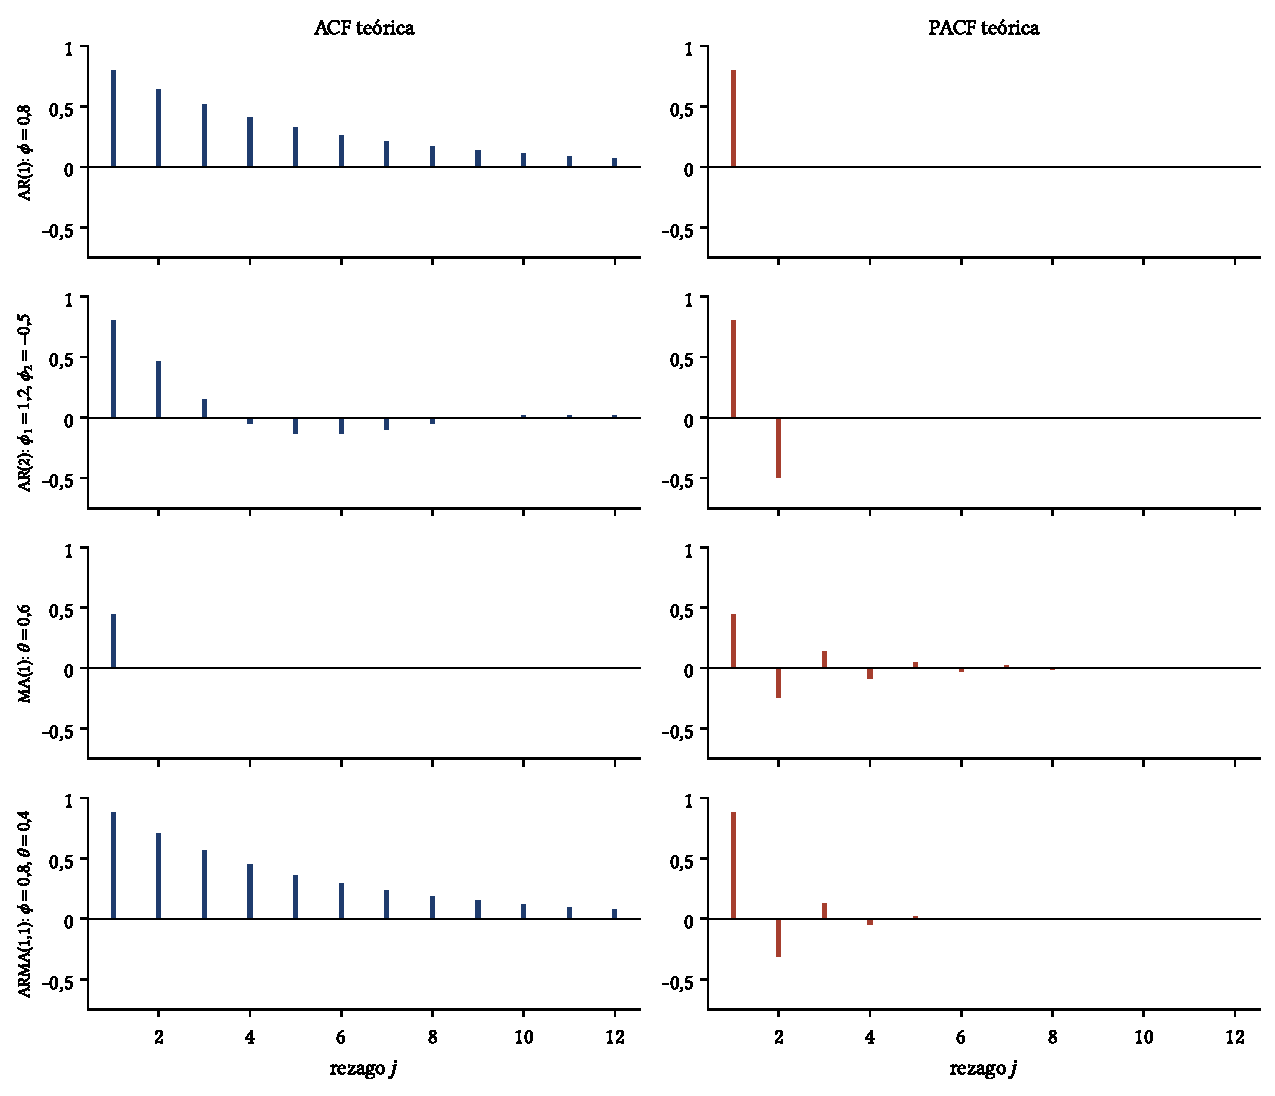
\includegraphics[width=0.92\linewidth]{graficos/cap06_fig_identificacion.pdf}
\caption{ACF (azul) y PACF (rojo) teóricas. El AR(1) tiene una ACF que decae geométricamente y una PACF con
una sola barra. El AR(2) con raíces complejas oscila. El MA(1) tiene una sola barra en la ACF y una PACF que
decae alternando de signo. El ARMA(1,1) combina ambos: las dos funciones decaen.}
\label{fig:identificacion}
\end{figure}

% ---------------------------------------------------------------------
\section{Estimación, selección y diagnóstico}
% ---------------------------------------------------------------------

\begin{proposicion}[MCO y máxima verosimilitud condicional en un AR]\label{prop:mvar}
Si $\varepsilon_t\sim N(0,\sigma^2)$, maximizar la verosimilitud del AR($p$) condicional en las primeras $p$
observaciones equivale a estimar por MCO la regresión de $y_t$ sobre una constante y $y_{t-1},\dots,y_{t-p}$.
\end{proposicion}

\begin{proof}
Condicional en el pasado, $y_t\sim N(c+\sum_j\phi_jy_{t-j},\ \sigma^2)$. La log-verosimilitud de
$y_{p+1},\dots,y_T$ es la suma de las log-densidades:
\begin{align*}
  \ell(c,\bm\phi,\sigma^2) &= \sum_{t=p+1}^T\Bigl[-\tfrac12\ln(2\pi\sigma^2)
                              -\frac{\bigl(y_t-c-\sum_j\phi_jy_{t-j}\bigr)^2}{2\sigma^2}\Bigr]\\
                           &= -\frac{T-p}{2}\ln(2\pi\sigma^2)-\frac{1}{2\sigma^2}\,\mathrm{SRC}(c,\bm\phi).
\end{align*}
Para cualquier $\sigma^2$, $\ell$ se maximiza en $(c,\bm\phi)$ minimizando $\mathrm{SRC}$, que es el problema
de MCO.
\end{proof}

Con términos de media móvil, los residuos dependen de los parámetros de forma no lineal
($\varepsilon_t=y_t-c-\phi y_{t-1}-\theta\varepsilon_{t-1}$), y la verosimilitud se maximiza numéricamente. R
(\texttt{arima}) y \texttt{statsmodels} (\texttt{ARIMA}) calculan la verosimilitud \emph{exacta} con el filtro
de Kalman; usan optimizadores distintos, por lo que sus estimaciones pueden diferir en la cuarta cifra
decimal.

\subsection{El sesgo de muestras finitas}

MCO es consistente en un AR(1) estacionario, pero sesgado en muestras finitas. Kendall (1954) mostró que, con
constante,
\[
  \E[\hat\phi]-\phi\approx-\frac{1+3\phi}{T}.
\]
El sesgo es negativo y crece con $\phi$: las series persistentes parecen menos persistentes de lo que son. La
Figura~\ref{fig:kendall} compara la fórmula con una simulación: es precisa hasta $\phi\approx0{,}9$ y
subestima el sesgo cerca de la raíz unitaria (con $\phi=0{,}99$ y $T=100$, la simulación da $-0{,}050$ y la
fórmula $-0{,}040$).

\begin{figure}[ht]
\centering
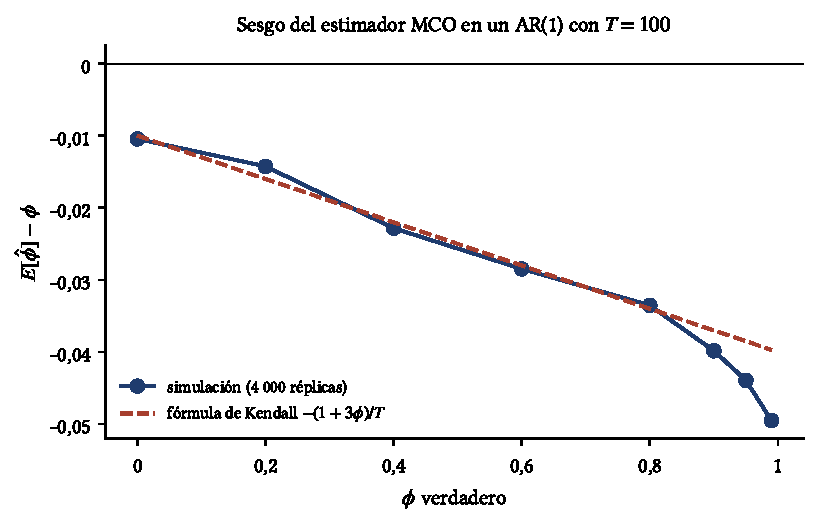
\includegraphics[width=0.72\linewidth]{graficos/cap06_fig_kendall.pdf}
\caption{Sesgo del estimador MCO de $\phi$ en un AR(1) con constante y $T=100$: simulación (puntos) y
aproximación de Kendall (línea discontinua).}
\label{fig:kendall}
\end{figure}

\begin{proposicion}[Sesgo de Stambaugh]\label{prop:stambaugh}
Considere la regresión predictiva y la dinámica del predictor
\begin{align*}
  r_{t+1} &= a+b\,x_t+u_{t+1},\\
  x_{t+1} &= c+\phi\,x_t+v_{t+1},
\end{align*}
con $(u_t,v_t)$ i.i.d. normales, de covarianza $\sigma_{uv}$, y $\sigma_v^2=\Var(v_t)$. Entonces
\[
  \E[\hat b-b]=\frac{\sigma_{uv}}{\sigma_v^2}\;\E[\hat\phi-\phi].
\]
\end{proposicion}

\begin{proof}
Proyectamos $u$ sobre $v$: $u_t=k\,v_t+\eta_t$ con $k=\sigma_{uv}/\sigma_v^2$ y $\eta_t$ independiente de toda
la sucesión $\{v_t\}$, y por tanto de toda la trayectoria de $x$. Con $S_{xx}=\sum_t(x_t-\bar x)^2$ y las sumas
sobre $t=1,\dots,T-1$, los estimadores MCO cumplen
\begin{align*}
  \hat b-b       &= \frac{\sum_t(x_t-\bar x)\,u_{t+1}}{S_{xx}},\\
  \hat\phi-\phi  &= \frac{\sum_t(x_t-\bar x)\,v_{t+1}}{S_{xx}}.
\end{align*}
Sustituyendo $u_{t+1}=k\,v_{t+1}+\eta_{t+1}$:
\begin{align*}
  \hat b-b &= k\,\frac{\sum_t(x_t-\bar x)\,v_{t+1}}{S_{xx}}+\frac{\sum_t(x_t-\bar x)\,\eta_{t+1}}{S_{xx}}\\
           &= k\,(\hat\phi-\phi)+\frac{\sum_t(x_t-\bar x)\,\eta_{t+1}}{S_{xx}} .
\end{align*}
Como $\eta$ es independiente de $x$, el segundo término tiene esperanza cero condicional en $x$. Tomando
esperanzas:
\begin{align*}
  \E[\hat b-b] &= k\,\E[\hat\phi-\phi]\\
               &= \frac{\sigma_{uv}}{\sigma_v^2}\,\E[\hat\phi-\phi]. && \qedhere
\end{align*}
\end{proof}

Con la razón dividendo/precio, $\sigma_{uv}<0$: cuando suben los precios, sube el rendimiento ($u>0$) y cae la
razón ($v<0$). Como $\E[\hat\phi-\phi]<0$, el sesgo de $\hat b$ es \emph{positivo}: la regresión exagera la
capacidad predictiva.

\subsection{Selección y diagnóstico}

Con $\hat\ell$ la log-verosimilitud maximizada y $k$ el número de parámetros, los criterios de información son
\[
  \mathrm{AIC}=-2\hat\ell+2k,\qquad \mathrm{BIC}=-2\hat\ell+k\ln T,
\]
y se elige el modelo con el menor valor. El BIC penaliza más los parámetros y, si el modelo verdadero está entre
los candidatos, lo elige con probabilidad que tiende a 1; el AIC tiende a elegir modelos algo más grandes, lo
que puede ser conveniente para pronosticar. Una vez elegido el modelo, sus residuos deben parecer ruido blanco:
se aplica la prueba de Ljung-Box con $m-p-q$ grados de libertad.

% ---------------------------------------------------------------------
\section{Pronóstico}
% ---------------------------------------------------------------------

El pronóstico que minimiza el error cuadrático medio es la esperanza condicional,
$\hat y_{T+h}=\E[y_{T+h}\mid y_T,y_{T-1},\dots]$.

\begin{proposicion}[Pronóstico de un AR(1)]\label{prop:pronar1}
En un AR(1) estacionario con media $\mu$:
\begin{align*}
  \hat y_{T+h} &= \mu+\phi^h\,(y_T-\mu),\\
  \E\bigl[(y_{T+h}-\hat y_{T+h})^2\bigr] &= \sigma^2\,\frac{1-\phi^{2h}}{1-\phi^2}.
\end{align*}
\end{proposicion}

\begin{proof}
Como en la Proposición~\ref{prop:vidamedia}, escribiendo $c=\mu(1-\phi)$:
\begin{align*}
  y_{T+h}-\mu &= \phi^h\,(y_T-\mu)+\sum_{i=0}^{h-1}\phi^{\,i}\,\varepsilon_{T+h-i}.
\end{align*}
Los choques futuros tienen esperanza condicional cero, de donde sale el pronóstico. El error es la suma de
choques futuros, que no están correlacionados:
\begin{align*}
  \E\bigl[(y_{T+h}-\hat y_{T+h})^2\bigr] &= \Var\Bigl(\sum_{i=0}^{h-1}\phi^{\,i}\,\varepsilon_{T+h-i}\Bigr)\\
                                         &= \sigma^2\sum_{i=0}^{h-1}\phi^{2i}\\
                                         &= \sigma^2\,\frac{1-\phi^{2h}}{1-\phi^2}. && \qedhere
\end{align*}
\end{proof}

Cuando $h\to\infty$, el pronóstico tiende a la media $\mu$ y el error cuadrático medio, a la varianza no
condicional $\sigma^2/(1-\phi^2)$: a horizontes largos, el mejor pronóstico es la media y el modelo ya no
aporta información. La Figura~\ref{fig:pronar1} muestra que la velocidad de ese proceso depende de $\phi$.

\begin{figure}[ht]
\centering
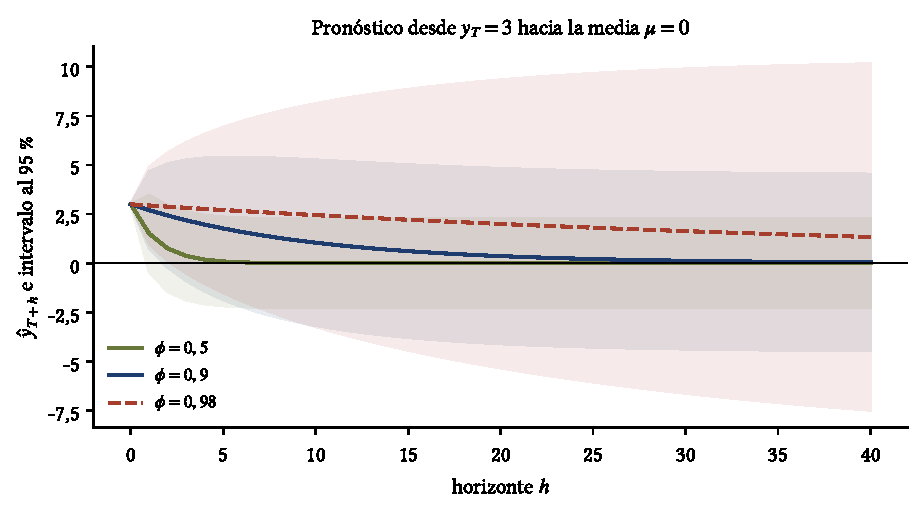
\includegraphics[width=0.78\linewidth]{graficos/cap06_fig_pronostico_ar1.pdf}
\caption{Pronóstico de un AR(1) desde $y_T=3$ con su intervalo al 95\,\% (bandas). Con $\phi=0{,}5$ el
pronóstico vuelve a la media en pocos períodos; con $\phi=0{,}98$ tarda mucho, y el intervalo se ensancha
hasta su límite $\pm1{,}96\,\sigma/\sqrt{1-\phi^2}$.}
\label{fig:pronar1}
\end{figure}

Para un ARMA(1,1), el pronóstico a un paso incorpora el último choque y los siguientes decaen como en el AR(1):
\begin{align*}
  \hat y_{T+1} &= \mu+\phi\,(y_T-\mu)+\theta\,\hat\varepsilon_T,\\
  \hat y_{T+h} &= \mu+\phi^{h-1}\,(\hat y_{T+1}-\mu),\\
  \E\bigl[(y_{T+h}-\hat y_{T+h})^2\bigr] &= \sigma^2\sum_{j=0}^{h-1}\psi_j^2,\qquad \psi_0=1,\quad \psi_j=\phi^{j-1}(\phi+\theta),
\end{align*}
donde los $\psi_j$ son los coeficientes de la representación $y_t=\mu+\sum_{j\ge0}\psi_j\varepsilon_{t-j}$.

\begin{definicion}[Prueba de Diebold-Mariano]
Para comparar dos pronósticos con errores $e_{1t}$ y $e_{2t}$, se define la diferencia de pérdidas
$d_t=e_{1t}^2-e_{2t}^2$ y el estadístico
\[
  DM=\frac{\bar d}{\sqrt{\hat S_d/n}},
\]
donde $\hat S_d$ es la varianza de largo plazo de $d_t$, estimada con Newey-West y $L=h-1$ rezagos (los errores
de pronóstico a $h$ pasos están autocorrelacionados hasta el rezago $h-1$). Bajo la hipótesis de igual
precisión, $DM\to N(0,1)$ (Diebold y Mariano, 1995).
\end{definicion}

% ---------------------------------------------------------------------
\section{Ejercicios resueltos}
% ---------------------------------------------------------------------

\begin{ejresuelto}{Identificación: los cambios de la tasa de interés a 10 años}\label{ej:tasaarma}
\enunciado Con los cambios mensuales del rendimiento del bono a 10 años (1953--2023): (a) calcule la ACF y la
PACF y proponga modelos candidatos; (b) estime AR(1), AR(2), MA(1), MA(2) y ARMA(1,1) por máxima verosimilitud
y compárelos con AIC y BIC; (c) relacione el resultado con el efecto de Working.

\solucion
\paso{Paso 1. ACF y PACF.} Con $T=845$, la banda al 95\,\% es $\pm0{,}067$. La ACF tiene un valor grande en el
primer rezago ($0{,}310$) y valores pequeños después; la PACF alterna de signo ($0{,}310$; $-0{,}212$;
$0{,}081$\ldots). El patrón ``ACF que se corta, PACF que decae alternando'' apunta a un MA(1)
(Figura~\ref{fig:identificacion}).

\paso{Paso 2. Comparación.} Los criterios de información, de menor a mayor (mejor primero):
\begin{center}\small
\begin{tabular}{@{}lrr@{}}
\toprule
Modelo & AIC & BIC \\
\midrule
MA(2)      & 17,45 & 36,41 \\
ARMA(1,1)  & 18,13 & 37,09 \\
MA(1)      & 23,27 & 37,49 \\
AR(2)      & 27,41 & 46,37 \\
AR(1)      & 64,33 & 78,55 \\
\bottomrule
\end{tabular}
\end{center}
Los dos criterios eligen el MA(2), pero las diferencias con el ARMA(1,1) y, para el BIC, con el MA(1) son
pequeñas. Los modelos autorregresivos puros quedan claramente atrás.

\paso{Paso 3. Working.} El MA(1) estimado tiene $\hat\theta=0{,}4454$, que implica
\begin{align*}
  \rho_1 &= \frac{\hat\theta}{1+\hat\theta^2}\\
         &= \frac{0{,}4454}{1+0{,}1984}\\
         &= \frac{0{,}4454}{1{,}1984}\\
         &= 0{,}372 .
\end{align*}
Si la tasa fuera un paseo aleatorio y solo se observara su promedio mensual, la Proposición~\ref{prop:workingma}
predice $\theta=0{,}268$ y $\rho_1=0{,}25$. La autocorrelación de los cambios mensuales se explica en buena
parte, aunque no del todo, porque la serie es un promedio de datos diarios.

\codigoweb{cap06_ej01}
\salidaR{cap06_ej01_R.txt}
\lectura{cap06_ej01}

\RvsPy \texttt{arima()} de R y \texttt{ARIMA} de \texttt{statsmodels} maximizan la misma verosimilitud exacta y
aquí coinciden en todas las cifras. Cambian los nombres: \texttt{ar1}, \texttt{ma1} e \texttt{intercept} en R;
\texttt{ar.L1}, \texttt{ma.L1} y \texttt{const} en Python. En los dos, la ``constante'' reportada es la
\emph{media} del proceso, no el término $c$ de la ecuación.

\begin{figure}[ht]
\centering
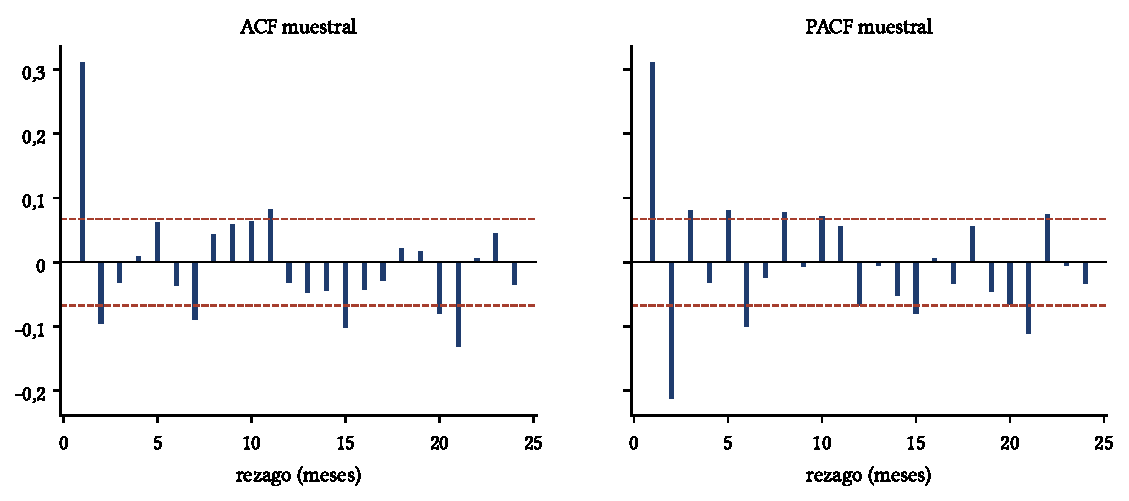
\includegraphics[width=0.92\linewidth]{graficos/cap06_fig_tasa_acf.pdf}
\caption{ACF y PACF muestrales de los cambios mensuales de la tasa a 10 años, con la banda al 95\,\%.}
\label{fig:tasaacf}
\end{figure}

\begin{conclusion}
Los cambios mensuales de la tasa a 10 años siguen aproximadamente un proceso de medias móviles de orden bajo.
Buena parte de esa dependencia es un artefacto de promediar: no es una oportunidad para predecir la dirección
de las tasas.
\end{conclusion}
\end{ejresuelto}

\begin{ejresuelto}{Estimación y diagnóstico: el logaritmo del VIX}\label{ej:vixarma}
\enunciado Estime AR(1), AR(2) y ARMA(1,1) para el logaritmo del VIX (1990--2026). Compare los criterios de
información, aplique la prueba de Ljung-Box a los residuos y calcule la vida media del modelo elegido.

\solucion
\paso{Paso 1. Selección.} AIC y BIC eligen el ARMA(1,1) ($-23\,678{,}75$ y $-23\,650{,}20$), con
$\hat\phi=0{,}9832$ y $\hat\theta=-0{,}0844$; ambos coeficientes son muy significativos
($\operatorname{ee}=0{,}0019$ y $0{,}0112$).

\paso{Paso 2. Diagnóstico.} Incluso en el mejor modelo, los residuos siguen autocorrelacionados:
$Q(10)=73{,}2$ con 8 grados de libertad, $p\approx10^{-12}$. Los demás modelos están peor. La
Figura~\ref{fig:vixresid} muestra que el AR(1) deja una autocorrelación negativa en los primeros rezagos, que
el ARMA(1,1) corrige en parte, pero quedan autocorrelaciones pequeñas y persistentes.

\paso{Paso 3. Vida media.}
\begin{align*}
  h^* &= \frac{\ln0{,}5}{\ln\hat\phi}\\
      &= \frac{-0{,}69315}{\ln0{,}9832}\\
      &= \frac{-0{,}69315}{-0{,}016943}\\
      &= 40{,}9 \text{ días}.
\end{align*}

\codigoweb{cap06_ej02}
\salidaR{cap06_ej02_R.txt}
\lectura{cap06_ej02}

\RvsPy Tres detalles hacen que las dos salidas sean comparables. Primero, \texttt{statsmodels} calcula por
defecto los errores estándar con el producto externo del gradiente; con \texttt{cov\_type="approx"} usa el
hessiano numérico, como R. Segundo, el primer residuo depende de cómo cada programa inicializa el filtro de
Kalman, así que lo excluimos en ambos. Tercero, los optimizadores difieren: $\hat\phi$ es $0{,}9832$ en R y
$0{,}9831$ en Python, lo que mueve la vida media entre $40{,}9$ y $40{,}6$ días. Diferencias de este tamaño son
normales en estimaciones no lineales y no cambian ninguna conclusión.

\begin{figure}[ht]
\centering
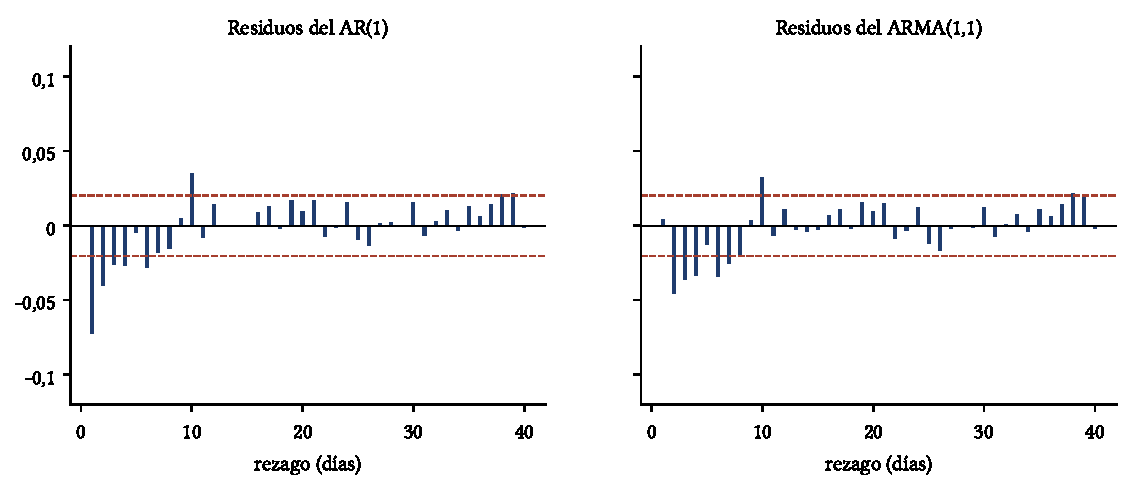
\includegraphics[width=0.92\linewidth]{graficos/cap06_fig_vix_resid.pdf}
\caption{ACF de los residuos del AR(1) y del ARMA(1,1) para el logaritmo del VIX, con la banda al 95\,\%.}
\label{fig:vixresid}
\end{figure}

\begin{conclusion}
El ARMA(1,1) es el mejor de los modelos ARMA de orden bajo para el VIX, pero no captura toda su dependencia,
en línea con la memoria larga detectada en el Ejercicio~\ref{ej:vixur}. Un modelo puede ser el mejor de los
candidatos y aun así ser inadecuado; el diagnóstico de residuos es lo que lo revela.
\end{conclusion}
\end{ejresuelto}

\begin{ejresuelto}{¿Supera el ARMA a un paseo aleatorio? Evaluación fuera de muestra}\label{ej:vixfuera}
\enunciado Estime el ARMA(1,1) del logaritmo del VIX con datos de 1990 a 2015. Con esos parámetros fijos,
pronostique a 1, 5 y 22 días desde cada día de 2016 a 2026, y compare con el paseo aleatorio (pronóstico igual
al último valor) y con la media de la muestra de estimación. Use la prueba de Diebold-Mariano.

\solucion
\paso{Paso 1. Parámetros.} Con datos hasta el 31 de diciembre de 2015: $\hat\mu=2{,}9228$, $\hat\phi=0{,}9861$ y
$\hat\theta=-0{,}0902$. Hay 2\,728 orígenes de pronóstico.

\paso{Paso 2. Precisión.} La raíz del error cuadrático medio (RECM), en puntos logarítmicos:
\begin{center}\small
\begin{tabular}{@{}rrrrrr@{}}
\toprule
$h$ & ARMA(1,1) & Paseo aleatorio & Media & ARMA/paseo & $DM$ \\
\midrule
1  & 0,0785 & 0,0792 & 0,3301 & 0,991 & 2,62 \\
5  & 0,1537 & 0,1579 & 0,3302 & 0,974 & 5,02 \\
22 & 0,2415 & 0,2630 & 0,3306 & 0,918 & 3,80 \\
\bottomrule
\end{tabular}
\end{center}
A 22 días, la mejora sobre el paseo aleatorio es de
\begin{align*}
  1-\frac{0{,}2415}{0{,}2630} &= 1-0{,}918\\
                              &= 0{,}082,
\end{align*}
es decir, un 8,2\,\% menos de error. A un día la mejora es menor del 1\,\%.

\paso{Paso 3. Significancia.} Los tres estadísticos $DM$ superan 1,96: el ARMA es significativamente más
preciso que el paseo aleatorio en los tres horizontes. Usar la media histórica es mucho peor que ambos.

\codigoweb{cap06_ej03}
\salidaR{cap06_ej03_R.txt}
\lectura{cap06_ej03}

\RvsPy Programamos la recursión de los residuos y los pronósticos a mano para que sean visibles las ecuaciones
de la sección de pronóstico. Las pequeñas diferencias en los parámetros (cuarta cifra decimal) se trasladan a
la tercera cifra del cociente a 5 días ($0{,}974$ frente a $0{,}973$) y a la segunda del estadístico $DM$.

\begin{figure}[ht]
\centering
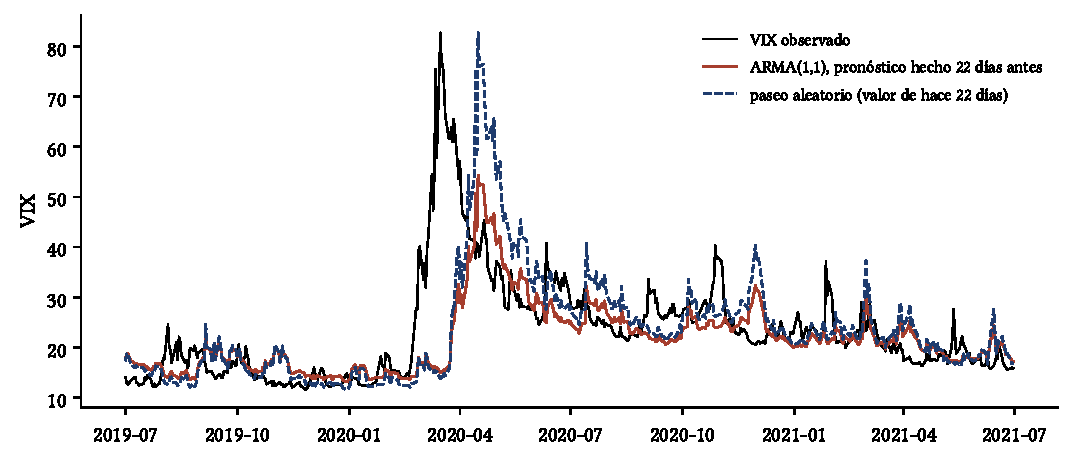
\includegraphics[width=0.92\linewidth]{graficos/cap06_fig_vix_pronostico.pdf}
\caption{Pronósticos a 22 días del VIX entre julio de 2019 y junio de 2021. Ningún modelo anticipa el salto de
marzo de 2020; después del salto, el ARMA(1,1) prevé la caída del VIX hacia su media, mientras que el paseo
aleatorio repite el nivel de crisis de 22 días antes.}
\label{fig:vixfuera}
\end{figure}

\begin{conclusion}
La reversión a la media del VIX es explotable para pronosticar: el ARMA(1,1) mejora al paseo aleatorio, sobre
todo a horizontes de un mes. Pero ningún modelo lineal anticipa los saltos; lo que hace mejor es prever su
disipación.
\end{conclusion}
\end{ejresuelto}

\begin{ejresuelto}{Pronóstico del VIX con intervalos de confianza}\label{ej:vixabanico}
\enunciado Con el ARMA(1,1) estimado con toda la muestra, pronostique el VIX desde el 22 de septiembre de 2026
hasta 60 días hábiles adelante, con intervalos al 95\,\%, y calcule el nivel de largo plazo.

\solucion
\paso{Paso 1. Pronóstico puntual.} El pronóstico del logaritmo es $\hat y_{T+h}=\hat\mu+\hat\phi^{h-1}(\hat y_{T+1}-\hat\mu)$,
y $e^{\hat y_{T+h}}$ es la mediana del pronóstico del VIX. Desde un nivel de 14,21, la mediana sube a 14,33
(1 día), 15,41 (22 días) y 16,70 (60 días), hacia el nivel de largo plazo
\begin{align*}
  e^{\hat\mu} &= e^{2{,}9042}\\
              &= 18{,}25 .
\end{align*}

\paso{Paso 2. Intervalos.} Con $\hat\sigma^2=0{,}004556$ y los pesos $\psi_j$, el intervalo al 95\,\% a 22 días es
$[9{,}50;\ 24{,}98]$ y a 60 días, $[8{,}98;\ 31{,}04]$. En el límite, el intervalo tiende a
$[9{,}39;\ 35{,}48]$.

\paso{Paso 3. Asimetría.} Los intervalos no son simétricos alrededor de la mediana: son simétricos en
logaritmos y, al exponenciar, la cola superior se alarga. Es coherente con la naturaleza del VIX, que puede
triplicarse en pocos días pero rara vez cae a la mitad.

\codigoweb{cap06_ej04}
\salidaR{cap06_ej04_R.txt}
\lectura{cap06_ej04}

\RvsPy Al final, la salida de Python compara nuestro cálculo con la función \texttt{get\_forecast} de
\texttt{statsmodels}, que reproduce la mediana a 22 días. En R se obtiene lo mismo con la función
\texttt{predict(m, n.ahead = 22)}.

\begin{figure}[ht]
\centering
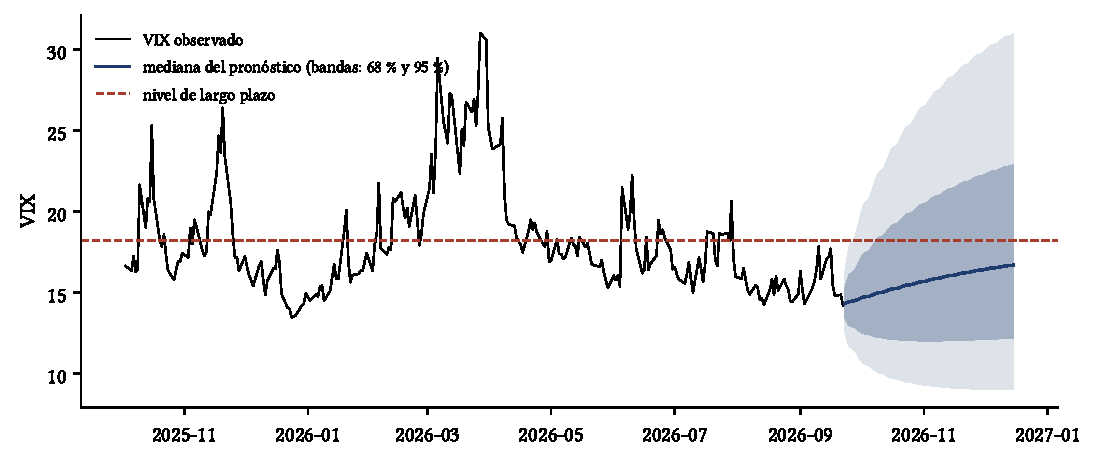
\includegraphics[width=0.92\linewidth]{graficos/cap06_fig_vix_abanico.pdf}
\caption{Último año del VIX y abanico de pronóstico a 60 días hábiles, con bandas al 68\,\% y al 95\,\%. La
mediana sube gradualmente hacia el nivel de largo plazo (línea discontinua), y la incertidumbre crece con el
horizonte, más hacia arriba que hacia abajo.}
\label{fig:vixabanico}
\end{figure}

\begin{conclusion}
Con un VIX por debajo de su media histórica, el modelo prevé un aumento gradual de la volatilidad implícita.
La amplitud del intervalo es la lección principal: a dos meses, valores entre 9 y 31 son compatibles con el
modelo.
\end{conclusion}
\end{ejresuelto}

\begin{ejresuelto}{El sesgo de Stambaugh en la predictibilidad de las acciones}\label{ej:stambaugh}
\enunciado Con datos mensuales de 1946 a 2023, estime la regresión del rendimiento total del S\&P 500 del mes
siguiente sobre $\ln(D_t/P_t)$ y el AR(1) del predictor. Calcule el sesgo de Kendall, el sesgo de Stambaugh y el
coeficiente corregido.

\solucion
\paso{Paso 1. Estimaciones.} Con $T=929$ meses: $\hat b=0{,}00611$ ($t=2{,}35$), aparentemente significativo
al 5\,\%; $\hat\phi=0{,}99759$; y la correlación entre las innovaciones es $-0{,}983$, con
$\hat k=\hat\sigma_{uv}/\hat\sigma_v^2=-0{,}9541$.

\paso{Paso 2. Sesgos.} Por la fórmula de Kendall y la Proposición~\ref{prop:stambaugh}:
\begin{align*}
  \text{sesgo de }\hat\phi &= -\frac{1+3\hat\phi}{T}\\
                           &= -\frac{1+3\times0{,}99759}{929}\\
                           &= -\frac{3{,}99277}{929}\\
                           &= -0{,}00430,\\
  \text{sesgo de }\hat b   &= \hat k\times(-0{,}00430)\\
                           &= -0{,}9541\times(-0{,}00430)\\
                           &= 0{,}00410 .
\end{align*}

\paso{Paso 3. Corrección.}
\begin{align*}
  \hat b_{\text{corregido}} &= \hat b-\text{sesgo de }\hat b\\
                            &= 0{,}00611-0{,}00410\\
                            &= 0{,}00201 .
\end{align*}
Dos tercios (67,1\,\%) del coeficiente estimado son sesgo. Además, como la fórmula de Kendall subestima el sesgo
cerca de la raíz unitaria (Figura~\ref{fig:kendall}), la corrección es conservadora: el coeficiente verdadero
probablemente es todavía menor.

\codigoweb{cap06_ej05}
\salidaR{cap06_ej05_R.txt}
\lectura{cap06_ej05}

\RvsPy El único cuidado es alinear las fechas: el rendimiento de $t$ a $t+1$ se regresa sobre la razón de $t$.
En R, \texttt{dp[-n]} quita el último valor y \texttt{dp[-1]} el primero; en Python, \texttt{dp[:-1]} y
\texttt{dp[1:]}.

\begin{figure}[ht]
\centering
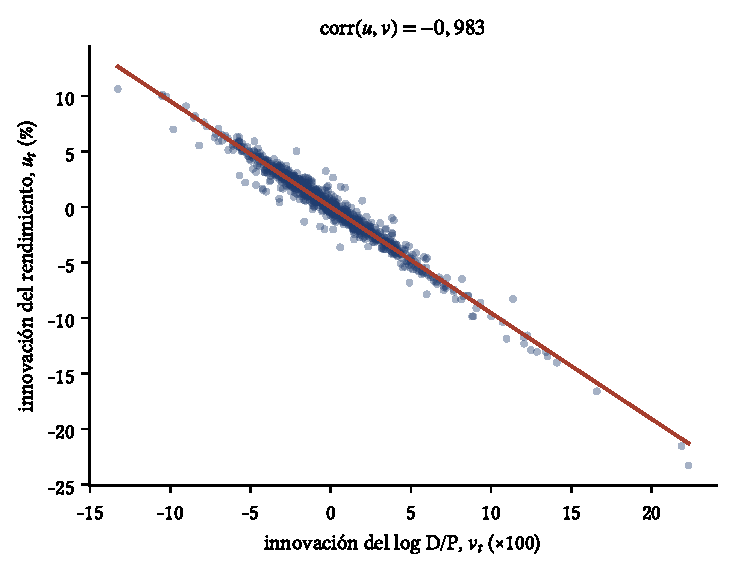
\includegraphics[width=0.62\linewidth]{graficos/cap06_fig_stambaugh.pdf}
\caption{Innovaciones del rendimiento frente a las del logaritmo de la razón dividendo/precio, 1946--2023. La
correlación es casi perfectamente negativa: cuando el mercado sube, la razón cae. Es esta relación, combinada con
la alta persistencia del predictor, la que produce el sesgo.}
\label{fig:stambaugh}
\end{figure}

\begin{conclusion}
La evidencia de predictibilidad con la razón dividendo/precio después de 1946 ($t=2{,}35$) es en buena parte un
sesgo de muestras finitas. Esta es la respuesta al Ejercicio propuesto~4.7: un estadístico $t$ alto no basta
cuando el predictor es muy persistente y sus innovaciones están correlacionadas con las del rendimiento.
\end{conclusion}
\end{ejresuelto}

% ---------------------------------------------------------------------
\section{Ejercicios propuestos}
% ---------------------------------------------------------------------

\begin{enumerate}[label=\textbf{\thechapter.\arabic*},leftmargin=*,itemsep=6pt]
  \item Derive la ACF de un MA(2) y demuestre que $\rho_j=0$ para $j\ge3$.
  \textit{Respuesta: $\rho_1=\theta_1(1+\theta_2)/(1+\theta_1^2+\theta_2^2)$, $\rho_2=\theta_2/(1+\theta_1^2+\theta_2^2)$.}

  \item Para el AR(2) con $\phi_1=1{,}2$ y $\phi_2=-0{,}5$, calcule $\rho_1$, $\rho_2$ y $\rho_3$, y las raíces de
  $1-1{,}2z+0{,}5z^2=0$. ¿Es estacionario? \textit{Respuesta: $\rho_1=0{,}8$, $\rho_2=0{,}46$, $\rho_3=0{,}152$;
  raíces $1{,}2\pm0{,}748i$, de módulo $1{,}414>1$.}

  \item Demuestre que el pronóstico de un paseo aleatorio a cualquier horizonte es el último valor observado y
  que su error cuadrático medio es $h\sigma^2$, que crece sin límite.

  \item Demuestre la fórmula de los pesos $\psi_j$ del ARMA(1,1) igualando coeficientes en
  $(1-\phi L)\sum_j\psi_jL^j=1+\theta L$.

  \item \emph{(Con datos.)} Repita el Ejercicio~\ref{ej:vixfuera} reestimando el ARMA(1,1) cada año (ventana
  creciente). ¿Mejora el pronóstico?

  \item \emph{(Con datos.)} Calcule la inflación mensual de EE.\,UU. desde 1953 con el IPC de la base de Shiller.
  Identifique un modelo ARMA. ¿Qué patrón aparece en el rezago 12 de la ACF y por qué?

  \item \emph{(Con datos del BCRP.)} Identifique y estime un modelo ARMA para la inflación mensual de Lima
  Metropolitana. Pronostique la inflación de los próximos 12 meses con intervalos y compárela con la meta de
  inflación del BCRP.

  \item \emph{(Simulación.)} Simule 2\,000 muestras con el modelo de la Proposición~\ref{prop:stambaugh},
  $b=0$, $\phi=0{,}99$, $T=300$ y $\operatorname{corr}(u,v)=-0{,}9$. ¿Con qué frecuencia rechaza la prueba $t$
  de $b=0$ al 5\,\% (a una cola)?
\end{enumerate}

% ---------------------------------------------------------------------
\section{Resumen de fórmulas}
% ---------------------------------------------------------------------

\begin{table}[H]
\centering\small
\begin{tabular}{@{}ll@{}}
\toprule
Concepto & Fórmula \\
\midrule
MA(1) & $\gamma_0=\sigma^2(1+\theta^2)$;\quad $\rho_1=\theta/(1+\theta^2)$;\quad $|\rho_1|\le1/2$ \\
Efecto de Working & $\theta=2-\sqrt3$ \\
AR(2) & $\rho_1=\phi_1/(1-\phi_2)$;\quad $\rho_j=\phi_1\rho_{j-1}+\phi_2\rho_{j-2}$ \\
ARMA(1,1) & $\rho_1=\frac{(1+\phi\theta)(\phi+\theta)}{1+2\phi\theta+\theta^2}$;\quad $\rho_j=\phi\rho_{j-1}$ \\
Sesgo de Kendall & $\E[\hat\phi]-\phi\approx-(1+3\phi)/T$ \\
Sesgo de Stambaugh & $\E[\hat b-b]=(\sigma_{uv}/\sigma_v^2)\,\E[\hat\phi-\phi]$ \\
Criterios de información & $\mathrm{AIC}=-2\hat\ell+2k$;\quad $\mathrm{BIC}=-2\hat\ell+k\ln T$ \\
Pronóstico AR(1) & $\hat y_{T+h}=\mu+\phi^h(y_T-\mu)$;\quad ECM $=\sigma^2(1-\phi^{2h})/(1-\phi^2)$ \\
Diebold-Mariano & $DM=\bar d/\sqrt{\hat S_d/n}\to N(0,1)$ \\
\bottomrule
\end{tabular}
\caption{Fórmulas principales del Capítulo 6.}
\end{table}

\section*{Referencias}
\begin{itemize}[leftmargin=*]
  \item Box, G. E. P. y Jenkins, G. M. (1970). \emph{Time Series Analysis: Forecasting and Control}.
        Holden-Day.
  \item Diebold, F. X. y Mariano, R. S. (1995). Comparing predictive accuracy. \emph{Journal of Business \&
        Economic Statistics}, 13(3), 253--263.
  \item Hamilton, J. D. (1994). \emph{Time Series Analysis}. Princeton University Press. Capítulos 3 a 5.
  \item Kendall, M. G. (1954). Note on bias in the estimation of autocorrelation. \emph{Biometrika},
        41(3--4), 403--404.
  \item Stambaugh, R. F. (1999). Predictive regressions. \emph{Journal of Financial Economics}, 54(3),
        375--421.
\end{itemize}

% =====================================================================
%  Capítulo 7. Eficiencia de mercado y predictibilidad
% =====================================================================
\chapter[Eficiencia de mercado]{Eficiencia de mercado: paseo aleatorio, razón de varianzas y anomalías}\label{cap:eficiencia}

\section*{Objetivos de aprendizaje}
Al terminar este capítulo, el lector podrá:
\begin{enumerate}[label=\arabic*.,leftmargin=*]
  \item Distinguir las tres formas de la hipótesis de mercado eficiente y las tres versiones de la hipótesis
        del paseo aleatorio, y explicar el problema de la hipótesis conjunta.
  \item Demostrar la relación entre la razón de varianzas y las autocorrelaciones, derivar su distribución
        asintótica y aplicar las pruebas $z$ y $z^*$ de Lo y MacKinlay.
  \item Interpretar la reversión a la media de largo plazo con el modelo de Poterba y Summers y reconocer la
        baja potencia de las pruebas de horizonte largo.
  \item Aplicar la prueba de rachas y explicar la autocorrelación de las carteras pequeñas mediante el ajuste
        parcial de precios y la negociación no sincrónica.
  \item Evaluar una anomalía (el momentum) con errores estándar robustos y medidas de riesgo de cola.
\end{enumerate}

\section*{Motivación}
Si los precios incorporan de inmediato toda la información disponible, los cambios de precio solo pueden
deberse a información nueva, que por definición es impredecible. Esa es la idea de la \emph{eficiencia de
mercado}, y de ella se desprende una predicción comprobable: los rendimientos pasados no deberían ayudar a
predecir los futuros. En los Capítulos~\ref{cap:hechos} y~\ref{cap:robustos} vimos que los rendimientos diarios
casi no están autocorrelacionados, pero que su volatilidad sí es predecible. Este capítulo convierte esa
observación en pruebas formales con varios horizontes y estudia los casos en que la predicción sí parece posible.

\paragraph{Datos del capítulo.} Rendimientos diarios del Brent (1987--2026); rendimientos mensuales de las
carteras por tamaño y valor y del factor momentum de la base de Kenneth French (1949--2017); y rendimientos
reales totales anuales del S\&P 500 de la base de Shiller (1871--2023).

% ---------------------------------------------------------------------
\section{La hipótesis de mercado eficiente}
% ---------------------------------------------------------------------

\begin{definicion}[Mercado eficiente; Fama, 1970]
Un mercado es \emph{eficiente} respecto de un conjunto de información $\mathcal I_t$ si los precios reflejan
plenamente $\mathcal I_t$, de modo que ninguna estrategia basada en $\mathcal I_t$ obtiene rendimientos
ajustados por riesgo superiores a los normales. Según el conjunto de información se distinguen tres formas:
\begin{itemize}[leftmargin=*]
  \item \textbf{débil}: $\mathcal I_t$ contiene los precios y rendimientos pasados;
  \item \textbf{semifuerte}: $\mathcal I_t$ contiene toda la información pública (estados financieros,
        anuncios, datos macroeconómicos);
  \item \textbf{fuerte}: $\mathcal I_t$ contiene también la información privada.
\end{itemize}
\end{definicion}

Este capítulo trata la forma débil; la semifuerte se estudia con los estudios de eventos del
Capítulo~16. La definición menciona rendimientos ``normales'', y eso exige un modelo de equilibrio que diga
cuánto debe rendir un activo (por ejemplo, el CAPM del Capítulo~\ref{cap:capm}). Por eso toda prueba de
eficiencia es una \emph{prueba conjunta}: si se rechaza, puede fallar la eficiencia o puede fallar el modelo de
rendimiento esperado, y los datos no distinguen entre las dos causas. Es el \emph{problema de la hipótesis
conjunta}.

\subsection{Tres versiones del paseo aleatorio}

Sea $p_t$ el logaritmo del precio y $r_t=p_t-p_{t-1}=\mu+\varepsilon_t$. Campbell, Lo y MacKinlay (1997)
ordenan las hipótesis de la más exigente a la menos exigente:
\begin{center}\small
\begin{tabular}{@{}lll@{}}
\toprule
Versión & Supuesto sobre $\varepsilon_t$ & ¿Admite volatilidad predecible? \\
\midrule
RW1 & independientes e idénticamente distribuidos & no \\
RW2 & independientes, no necesariamente idénticos & solo cambios deterministas \\
RW3 & no correlacionados: $\Cov(\varepsilon_t,\varepsilon_{t-j})=0$ para $j\ne0$ & sí \\
\bottomrule
\end{tabular}
\end{center}
La Proposición~\ref{prop:mds} mostró que la falta de correlación no implica independencia. Los rendimientos
reales tienen agrupamiento de volatilidad, así que RW1 es falsa casi siempre; la hipótesis interesante es RW3,
o la versión más fuerte de que $r_t$ sea una \emph{diferencia de martingala} alrededor de $\mu$. Las pruebas de
este capítulo deben, por tanto, ser válidas bajo heterocedasticidad condicional.

\begin{proposicion}[Impredecibilidad bajo la martingala]\label{prop:martingala}
Si $\E[r_t\mid\mathcal F_{t-1}]=\mu$, donde $\mathcal F_{t-1}$ contiene los rendimientos pasados, entonces para
toda función $g$ de la información pasada con $\E[g^2]<\infty$,
\[
  \Cov\bigl(r_t,\ g(\mathcal F_{t-1})\bigr)=0 .
\]
En particular, $\Cov(r_t,r_{t-j})=0$ para todo $j\ge1$.
\end{proposicion}

\begin{proof}
Escribimos $g=g(\mathcal F_{t-1})$. Por la ley de esperanzas iteradas, y porque $g$ es conocida en $t-1$:
\begin{align*}
  \E[r_t\,g] &= \E\bigl[\E[r_t\,g\mid\mathcal F_{t-1}]\bigr]\\
             &= \E\bigl[g\,\E[r_t\mid\mathcal F_{t-1}]\bigr]\\
             &= \E[g\,\mu]\\
             &= \mu\,\E[g].
\end{align*}
Además $\E[r_t]=\E\bigl[\E[r_t\mid\mathcal F_{t-1}]\bigr]=\mu$. Entonces
\begin{align*}
  \Cov(r_t,g) &= \E[r_t\,g]-\E[r_t]\,\E[g]\\
              &= \mu\,\E[g]-\mu\,\E[g]\\
              &= 0 .
\end{align*}
Tomando $g=r_{t-j}$ se obtiene el caso particular.
\end{proof}

La proposición dice que ninguna regla de inversión basada en precios pasados, lineal o no lineal, predice el
rendimiento. Nótese que $g$ puede ser $r_{t-1}^2$: la volatilidad pasada no predice el \emph{nivel} del
rendimiento, aunque sí prediga su \emph{varianza}.

% ---------------------------------------------------------------------
\section{La razón de varianzas}
% ---------------------------------------------------------------------

Si los rendimientos no están correlacionados, la varianza de un rendimiento de $q$ períodos es $q$ veces la de
un período (Proposición~\ref{prop:agregmom}). La razón de varianzas mide cuánto se aparta un mercado de esa
regla.

\begin{definicion}[Razón de varianzas]
Para un rendimiento estacionario con varianza $\sigma^2$, la razón de varianzas de horizonte $q$ es
\[
  VR(q)=\frac{\Var\bigl[r_t(q)\bigr]}{q\,\Var[r_t]},\qquad r_t(q)=r_t+r_{t-1}+\dots+r_{t-q+1}.
\]
\end{definicion}

\begin{proposicion}[Razón de varianzas y autocorrelaciones]\label{prop:vrrho}
Con autocorrelaciones $\rho_j$,
\[
  VR(q)=1+2\sum_{j=1}^{q-1}\Bigl(1-\frac jq\Bigr)\rho_j .
\]
En particular, $VR(2)=1+\rho_1$, y bajo RW1, RW2 o RW3, $VR(q)=1$ para todo $q$.
\end{proposicion}

\begin{proof}
Por la Proposición~\ref{prop:agregmom}, con $k=q$,
\begin{align*}
  \Var\bigl[r_t(q)\bigr] &= \sigma^2\Bigl[q+2\sum_{j=1}^{q-1}(q-j)\rho_j\Bigr].
\end{align*}
Dividimos entre $q\sigma^2$:
\begin{align*}
  VR(q) &= \frac{\sigma^2\bigl[q+2\sum_{j=1}^{q-1}(q-j)\rho_j\bigr]}{q\sigma^2}\\
        &= \frac{q}{q}+\frac2q\sum_{j=1}^{q-1}(q-j)\rho_j\\
        &= 1+2\sum_{j=1}^{q-1}\frac{q-j}{q}\,\rho_j\\
        &= 1+2\sum_{j=1}^{q-1}\Bigl(1-\frac jq\Bigr)\rho_j .
\end{align*}
Para $q=2$ la suma tiene un solo término:
\begin{align*}
  VR(2) &= 1+2\Bigl(1-\frac12\Bigr)\rho_1\\
        &= 1+\rho_1 .
\end{align*}
Si $\rho_j=0$ para $j\ge1$, la suma se anula y $VR(q)=1$.
\end{proof}

$VR(q)$ es una combinación lineal de las primeras $q-1$ autocorrelaciones con pesos que decrecen linealmente.
Si $VR(q)>1$ predominan las autocorrelaciones positivas (inercia, \emph{momentum}); si $VR(q)<1$, las
negativas (reversión a la media). Su ventaja sobre las autocorrelaciones sueltas es que acumula muchas
autocorrelaciones pequeñas del mismo signo, difíciles de detectar una por una.

\begin{ejemplo}[Rendimientos AR(1)]\label{ej:vrar1}
Si $r_t$ sigue un AR(1), $\rho_j=\rho^j$ con $|\rho|<1$. Cuando $q\to\infty$, el peso $j/q$ de cada término
se anula y
\begin{align*}
  \lim_{q\to\infty}VR(q) &= 1+2\sum_{j=1}^{\infty}\rho^j\\
                         &= 1+\frac{2\rho}{1-\rho}\\
                         &= \frac{1-\rho+2\rho}{1-\rho}\\
                         &= \frac{1+\rho}{1-\rho}.
\end{align*}
Con $\rho=0{,}15$:
\begin{align*}
  \lim_{q\to\infty}VR(q) &= \frac{1{,}15}{0{,}85}\\
                         &= 1{,}353 .
\end{align*}
Con $\rho=-0{,}15$ el límite es $0{,}85/1{,}15=0{,}739$. Sumando las series geométricas finitas se obtiene la
fórmula exacta
\[
  VR(q)=\frac{1+\rho}{1-\rho}-\frac{2\rho\,(1-\rho^q)}{q\,(1-\rho)^2},
\]
que es la que dibuja el panel izquierdo de la Figura~\ref{fig:vrteoria}: la curva parte de $1+\rho$ en $q=2$ y
se aproxima con rapidez a su límite.
\end{ejemplo}

\begin{figure}[ht]
\centering
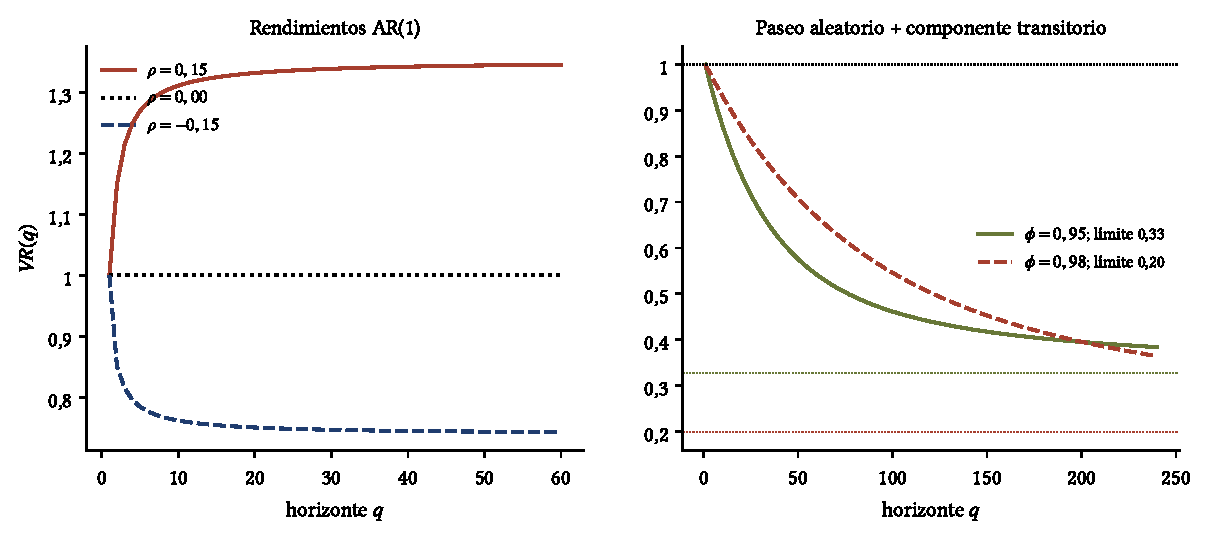
\includegraphics[width=\linewidth]{graficos/cap07_fig_vr_teoria.pdf}
\caption{Razón de varianzas teórica. Izquierda: rendimientos AR(1) con $\rho=0{,}15$, $0$ y $-0{,}15$; la
curva se estabiliza en $(1+\rho)/(1-\rho)$. Derecha: precio igual a un paseo aleatorio más un componente
transitorio AR(1) (Proposición~\ref{prop:poterba}); la curva desciende lentamente hacia el límite marcado con
línea punteada del mismo color.}
\label{fig:vrteoria}
\end{figure}

\subsection{El estimador de Lo y MacKinlay}

Sea una muestra de $T$ rendimientos $r_1,\dots,r_T$. Lo y MacKinlay (1988) usan los rendimientos de $q$
períodos \emph{traslapados}, uno por cada fecha, para no desperdiciar observaciones:
\begin{align*}
  \hat\mu &= \frac1T\sum_{t=1}^{T}r_t,\\
  \hat\sigma_a^2 &= \frac1{T-1}\sum_{t=1}^{T}(r_t-\hat\mu)^2,\\
  \hat\sigma_c^2(q) &= \frac1m\sum_{t=q}^{T}\bigl(r_t(q)-q\hat\mu\bigr)^2,
       \qquad m=q\,(T-q+1)\Bigl(1-\frac qT\Bigr),\\
  \widehat{VR}(q) &= \frac{\hat\sigma_c^2(q)}{\hat\sigma_a^2}.
\end{align*}
El divisor $m$ corrige el sesgo de muestra finita que producen el traslape y la estimación de la media.

\begin{proposicion}[Distribución bajo RW1]\label{prop:vrasint}
Bajo RW1,
\[
  \sqrt T\,\bigl(\widehat{VR}(q)-1\bigr)\xrightarrow{d}N\Bigl(0,\ \frac{2(2q-1)(q-1)}{3q}\Bigr),
  \qquad
  z(q)=\frac{\widehat{VR}(q)-1}{\sqrt{2(2q-1)(q-1)/(3qT)}}\xrightarrow{d}N(0,1).
\]
\end{proposicion}

\begin{proof}
En muestras grandes $\widehat{VR}(q)$ se comporta como su contraparte de la Proposición~\ref{prop:vrrho} con
las autocorrelaciones muestrales:
\begin{align*}
  \widehat{VR}(q)-1 &\approx 2\sum_{j=1}^{q-1}\Bigl(1-\frac jq\Bigr)\hat\rho_j .
\end{align*}
Bajo RW1, los $\sqrt T\hat\rho_j$ son asintóticamente $N(0,1)$ e independientes entre sí (resultado de
Bartlett, Capítulo~\ref{cap:hechos}). La varianza de una suma de variables independientes es la suma de las
varianzas:
\begin{align*}
  \Var\Bigl[\sqrt T\bigl(\widehat{VR}(q)-1\bigr)\Bigr]
    &\to 4\sum_{j=1}^{q-1}\Bigl(1-\frac jq\Bigr)^2\\
    &= \frac4{q^2}\sum_{j=1}^{q-1}(q-j)^2\\
    &= \frac4{q^2}\sum_{k=1}^{q-1}k^2 .
\end{align*}
En la última línea cambiamos el índice a $k=q-j$, que recorre $q-1,\dots,1$. Usamos
$\sum_{k=1}^{n}k^2=n(n+1)(2n+1)/6$ con $n=q-1$:
\begin{align*}
  \frac4{q^2}\sum_{k=1}^{q-1}k^2 &= \frac4{q^2}\cdot\frac{(q-1)\,q\,(2q-1)}{6}\\
                                 &= \frac{4\,(q-1)(2q-1)}{6q}\\
                                 &= \frac{2(2q-1)(q-1)}{3q}.
\end{align*}
La normalidad viene de que $\widehat{VR}(q)-1$ es asintóticamente una combinación lineal de normales. Dividir
entre la desviación estándar da $z(q)$.
\end{proof}

Para $q=2$ la varianza asintótica es $2\cdot3\cdot1/6=1$, lo mismo que la de $\sqrt T\hat\rho_1$, como debe
ser porque $\widehat{VR}(2)-1\approx\hat\rho_1$.

\subsection{La versión robusta a heterocedasticidad}

Con agrupamiento de volatilidad, la varianza de cada $\hat\rho_j$ es mayor que $1/T$
(Proposición~\ref{prop:acfrob}), y $z(q)$ rechaza la hipótesis cierta con demasiada frecuencia. Lo y MacKinlay
proponen sustituir cada $1/T$ por su versión robusta.

\begin{proposicion}[Estadístico robusto $z^*$]\label{prop:vrrob}
Si $r_t-\mu$ es una diferencia de martingala con cuarto momento finito y
$\E[(r_t-\mu)^2(r_{t-j}-\mu)(r_{t-k}-\mu)]=0$ para $j\ne k$, entonces
\begin{align*}
  z^*(q) &= \frac{\widehat{VR}(q)-1}{\sqrt{\hat\theta(q)/T}}\xrightarrow{d}N(0,1),\\
  \hat\theta(q) &= \sum_{j=1}^{q-1}\Bigl[\frac{2(q-j)}{q}\Bigr]^2\hat\delta_j,\\
  \hat\delta_j &= \frac{T\sum_{t=j+1}^{T}(r_t-\hat\mu)^2(r_{t-j}-\hat\mu)^2}
                     {\Bigl[\sum_{t=1}^{T}(r_t-\hat\mu)^2\Bigr]^2}.
\end{align*}
\end{proposicion}

\begin{proof}[Esbozo de demostración]
La aproximación lineal es la misma que en la Proposición~\ref{prop:vrasint}:
\begin{align*}
  \sqrt T\bigl(\widehat{VR}(q)-1\bigr) &\approx \sum_{j=1}^{q-1}\frac{2(q-j)}{q}\,\sqrt T\hat\rho_j .
\end{align*}
Por la Proposición~\ref{prop:acfrob}, $\sqrt T\hat\rho_j$ tiene varianza asintótica
$\delta_j=\E[\varepsilon_t^2\varepsilon_{t-j}^2]/\sigma^4$, que $\hat\delta_j$ estima de forma consistente. La
covarianza entre $\sqrt T\hat\rho_j$ y $\sqrt T\hat\rho_k$ es proporcional a
$\E[\varepsilon_t^2\varepsilon_{t-j}\varepsilon_{t-k}]$, que es cero por hipótesis. Sin covarianzas,
\begin{align*}
  \Var\Bigl[\sqrt T\bigl(\widehat{VR}(q)-1\bigr)\Bigr]
     &\to \sum_{j=1}^{q-1}\Bigl[\frac{2(q-j)}{q}\Bigr]^2\delta_j\\
     &= \theta(q).
\end{align*}
Bajo RW1, $\delta_j=1$ y $\theta(q)$ se reduce a la varianza de la Proposición~\ref{prop:vrasint}.
\end{proof}

¿Importa la diferencia? La Figura~\ref{fig:vrtamano} resume una simulación de 2\,000 muestras de $T=1\,000$
rendimientos GARCH(1,1) sin ninguna autocorrelación ($\omega=0{,}05$, $\alpha=0{,}10$, $\beta=0{,}85$), es decir,
con la hipótesis nula cierta. Una prueba al 5\,\% debería rechazar en el 5\,\% de las muestras. La prueba $z$
rechaza entre el $9{,}0$\,\% y el $10{,}4$\,\% de las veces, casi el doble; la prueba $z^*$ rechaza entre el
$5{,}0$\,\% y el $5{,}4$\,\%. Con datos financieros se usa siempre $z^*$.

\begin{figure}[ht]
\centering
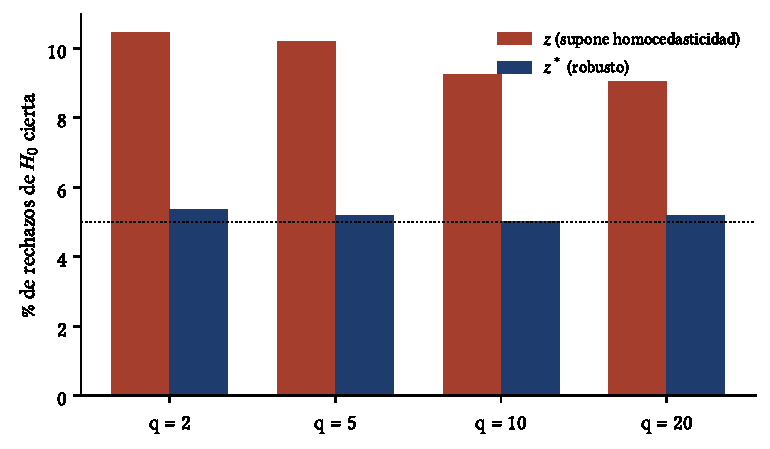
\includegraphics[width=0.66\linewidth]{graficos/cap07_fig_vr_tamano.pdf}
\caption{Porcentaje de rechazos de la hipótesis nula cierta (pruebas al 5\,\%) en 2\,000 muestras simuladas de
rendimientos GARCH(1,1) no autocorrelacionados con $T=1\,000$. La línea punteada marca el 5\,\% nominal.}
\label{fig:vrtamano}
\end{figure}

\begin{observacion}
Una prueba con un solo $q$ es fácil de interpretar, pero en la práctica se calculan varios. Probar cada uno al
5\,\% infla el error de tipo I conjunto. Chow y Denning (1993) proponen comparar $\max_q|z^*(q)|$ con un valor
crítico corregido; Kim (2006) propone un \emph{bootstrap} salvaje. Aquí reportamos las pruebas individuales y
las interpretamos con esa cautela.
\end{observacion}

% ---------------------------------------------------------------------
\section{Reversión a la media de largo plazo}
% ---------------------------------------------------------------------

Fama y French (1988) y Poterba y Summers (1988) encontraron que los rendimientos de las acciones a horizontes de
3 a 5 años tienen autocorrelación negativa: los períodos de rendimientos altos tienden a ser seguidos por
períodos bajos. El modelo más simple que produce ese patrón separa el precio en una parte permanente y otra
transitoria.

\begin{proposicion}[Poterba y Summers]\label{prop:poterba}
Sea $p_t=w_t+z_t$, donde $w_t=\mu+w_{t-1}+\eta_t$ es un paseo aleatorio con $\Var(\eta_t)=\sigma_w^2$ y
$z_t=\phi z_{t-1}+u_t$ es un AR(1) estacionario con $0<\phi<1$ y varianza $\gamma_0$, independiente de $w_t$.
Entonces
\[
  VR(k)=\frac{k\,\sigma_w^2+2\gamma_0(1-\phi^k)}{k\bigl[\sigma_w^2+2\gamma_0(1-\phi)\bigr]},
  \qquad
  \lim_{k\to\infty}VR(k)=\frac{\sigma_w^2}{\sigma_w^2+2\gamma_0(1-\phi)}<1 .
\]
\end{proposicion}

\begin{proof}
El rendimiento de $k$ períodos es la suma de los cambios de cada componente:
\begin{align*}
  r_t(k) &= p_t-p_{t-k}\\
         &= (w_t-w_{t-k})+(z_t-z_{t-k}).
\end{align*}
El primer término es una suma de $k$ innovaciones independientes más una constante:
\begin{align*}
  w_t-w_{t-k} &= k\mu+\sum_{i=0}^{k-1}\eta_{t-i},\\
  \Var(w_t-w_{t-k}) &= k\,\sigma_w^2 .
\end{align*}
Para el segundo usamos que $\Cov(z_t,z_{t-k})=\phi^k\gamma_0$ en un AR(1):
\begin{align*}
  \Var(z_t-z_{t-k}) &= \Var(z_t)+\Var(z_{t-k})-2\Cov(z_t,z_{t-k})\\
                    &= \gamma_0+\gamma_0-2\phi^k\gamma_0\\
                    &= 2\gamma_0(1-\phi^k).
\end{align*}
Como los componentes son independientes, las varianzas se suman:
\begin{align*}
  \Var\bigl[r_t(k)\bigr] &= k\,\sigma_w^2+2\gamma_0(1-\phi^k).
\end{align*}
Con $k=1$ se obtiene la varianza de un período:
\begin{align*}
  \Var[r_t] &= \sigma_w^2+2\gamma_0(1-\phi).
\end{align*}
Dividiendo la primera entre $k$ veces la segunda resulta la fórmula de $VR(k)$. Para el límite, escribimos
\begin{align*}
  VR(k) &= \frac{\sigma_w^2+2\gamma_0(1-\phi^k)/k}{\sigma_w^2+2\gamma_0(1-\phi)} .
\end{align*}
Como $0\le1-\phi^k\le1$, el término $2\gamma_0(1-\phi^k)/k$ tiende a cero y
\begin{align*}
  \lim_{k\to\infty}VR(k) &= \frac{\sigma_w^2}{\sigma_w^2+2\gamma_0(1-\phi)} .
\end{align*}
Es menor que uno porque $\gamma_0>0$ y $1-\phi>0$.
\end{proof}

A corto plazo el componente transitorio agrega varianza; a largo plazo sus efectos se cancelan (lo que sube por
$z_t$ luego baja) y solo queda la varianza del paseo aleatorio. El panel derecho de la Figura~\ref{fig:vrteoria}
lo ilustra con $\sigma_w^2=1$. Con $\phi=0{,}95$ y $\Var(u_t)=2$, la varianza del componente transitorio es
$\gamma_0=2/(1-0{,}95^2)=20{,}51$ y
\begin{align*}
  \lim_{k\to\infty}VR(k) &= \frac{1}{1+2(20{,}51)(0{,}05)}\\
                         &= \frac{1}{1+2{,}051}\\
                         &= 0{,}328 .
\end{align*}
Con $\phi=0{,}98$ y $\Var(u_t)=4$ el límite es $0{,}198$, pero la curva baja más despacio: cuanto más
persistente es el componente transitorio, más largo es el horizonte necesario para verlo.

\paragraph{El problema de la potencia.} Ver la reversión exige horizontes largos, y con horizontes largos hay
pocas observaciones independientes. Con 152 años de datos y $q=10$ hay apenas 15 décadas no traslapadas. Bajo
RW1 la desviación estándar de $\widehat{VR}(10)$ es
\begin{align*}
  \sqrt{\frac{2(2\cdot10-1)(10-1)}{3\cdot10\cdot152}}
    &= \sqrt{\frac{342}{4\,560}}\\
    &= \sqrt{0{,}075}\\
    &= 0{,}274,
\end{align*}
de modo que una razón de $0{,}5$ (una reversión enorme) apenas tendría $z=-1{,}83$. Las pruebas de horizonte
largo tienen poca potencia y, además, tienden a mostrar $\widehat{VR}<1$ incluso sin reversión, porque el
estimador está sesgado hacia abajo en muestras pequeñas (Richardson y Stock, 1989).

% ---------------------------------------------------------------------
\section{La prueba de rachas}
% ---------------------------------------------------------------------

La razón de varianzas usa la magnitud de los rendimientos. Una prueba no paramétrica que solo usa su
\emph{signo} es la de rachas de Wald y Wolfowitz (1940). Una \emph{racha} es una secuencia máxima de signos
iguales: la secuencia $+\,+\,-\,+\,+\,+\,-\,-$ tiene cuatro rachas. Si los rendimientos tienden a repetir su
signo hay pocas rachas largas; si tienden a alternar, hay muchas rachas cortas.

\begin{proposicion}[Número esperado de rachas]\label{prop:rachas}
Sea una secuencia de $n_1$ signos positivos y $n_2$ negativos, $n=n_1+n_2$, en la que todos los ordenamientos
son igualmente probables. El número de rachas $R$ cumple
\[
  \E[R]=\frac{2n_1n_2}{n}+1,\qquad
  \Var[R]=\frac{2n_1n_2\,(2n_1n_2-n)}{n^2(n-1)},
\]
y $Z=(R-\E[R])/\sqrt{\Var[R]}\xrightarrow{d}N(0,1)$ cuando $n_1,n_2\to\infty$.
\end{proposicion}

\begin{proof}[Demostración de la media]
Cada cambio de signo entre $t-1$ y $t$ inicia una racha nueva. Con $I_t=1$ si el signo en $t$ difiere del signo
en $t-1$ y $I_t=0$ en otro caso,
\begin{align*}
  R &= 1+\sum_{t=2}^{n}I_t .
\end{align*}
Las posiciones $t-1$ y $t$ forman un par al azar de los $n$ signos. Hay $n(n-1)$ pares ordenados posibles, y
$2n_1n_2$ de ellos tienen signos distintos ($n_1n_2$ con ``$+$ luego $-$'' y $n_2n_1$ con ``$-$ luego $+$''):
\begin{align*}
  \E[I_t] &= \Pr(\text{signos distintos en } t-1 \text{ y } t)\\
          &= \frac{2n_1n_2}{n(n-1)} .
\end{align*}
Por linealidad de la esperanza:
\begin{align*}
  \E[R] &= 1+\sum_{t=2}^{n}\E[I_t]\\
        &= 1+(n-1)\,\frac{2n_1n_2}{n(n-1)}\\
        &= 1+\frac{2n_1n_2}{n} .
\end{align*}
La varianza requiere las covarianzas entre los $I_t$ y se encuentra en Wald y Wolfowitz (1940).
\end{proof}

La prueba condiciona en $n_1$ y $n_2$, de modo que no le afecta que haya más días de subida que de bajada (una
deriva positiva). Un $Z$ negativo y significativo indica menos rachas de las esperadas, es decir, persistencia
del signo; uno positivo, alternancia.

% ---------------------------------------------------------------------
\section{Anomalías y fuentes de predictibilidad}
% ---------------------------------------------------------------------

\subsection{Ajuste parcial y negociación no sincrónica}

Lo y MacKinlay (1990) observaron que los rendimientos de las carteras de empresas pequeñas están
autocorrelacionados positivamente y que, además, los rendimientos pasados de las grandes predicen los de las
pequeñas, pero no al revés. Una explicación es que los precios de las acciones pequeñas, menos negociadas,
incorporan la información común con retraso.

\begin{proposicion}[Ajuste parcial]\label{prop:ajusteparcial}
Sea $f_t$ un factor común i.i.d. con media cero y varianza $\sigma^2$. La cartera grande refleja el factor de
inmediato, $r^G_t=f_t$, y la pequeña lo refleja en dos períodos,
\[
  r^P_t=a\,f_t+(1-a)\,f_{t-1},\qquad 0<a<1 .
\]
Entonces
\begin{align*}
  \operatorname{corr}(r^P_t,r^P_{t-1})&=\frac{a(1-a)}{a^2+(1-a)^2}>0, &
  \Cov(r^P_t,r^G_{t-1})&=(1-a)\sigma^2>0, &
  \Cov(r^G_t,r^P_{t-1})&=0 .
\end{align*}
\end{proposicion}

\begin{proof}
Como los $f_t$ no están correlacionados, solo sobreviven los productos con el mismo subíndice. La varianza de
la cartera pequeña es
\begin{align*}
  \Var(r^P_t) &= a^2\Var(f_t)+(1-a)^2\Var(f_{t-1})\\
              &= \bigl[a^2+(1-a)^2\bigr]\sigma^2 .
\end{align*}
Su autocovarianza de primer orden:
\begin{align*}
  \Cov(r^P_t,r^P_{t-1}) &= \Cov\bigl(a f_t+(1-a)f_{t-1},\ a f_{t-1}+(1-a)f_{t-2}\bigr)\\
                        &= (1-a)\,a\,\Var(f_{t-1})\\
                        &= a(1-a)\,\sigma^2 .
\end{align*}
Dividiendo entre la varianza se obtiene la autocorrelación. Las covarianzas cruzadas:
\begin{align*}
  \Cov(r^P_t,r^G_{t-1}) &= \Cov\bigl(a f_t+(1-a)f_{t-1},\ f_{t-1}\bigr)\\
                        &= (1-a)\,\sigma^2,\\[4pt]
  \Cov(r^G_t,r^P_{t-1}) &= \Cov\bigl(f_t,\ a f_{t-1}+(1-a)f_{t-2}\bigr)\\
                        &= 0 . \qedhere
\end{align*}
\end{proof}

El modelo explica a la vez la autocorrelación positiva de las carteras pequeñas y la \emph{asimetría} de las
correlaciones cruzadas, que veremos en el Ejercicio~\ref{ej:adelanto}. Con $a=0{,}7$, por ejemplo,
$\operatorname{corr}(r^P_t,r^P_{t-1})=0{,}21/0{,}58=0{,}362$. Esta predictibilidad es difícil de explotar: está
en acciones poco líquidas, con costos de transacción altos, y en parte es un artefacto de precios de cierre que
no corresponden a transacciones simultáneas.

\subsection{Momentum}

Jegadeesh y Titman (1993) mostraron que las acciones con mayores rendimientos en los últimos 3 a 12 meses
siguen rindiendo más que las de menores rendimientos durante los meses siguientes. El factor UMD (\emph{up
minus down}) de la base de French compra las acciones ganadoras y vende las perdedoras según el rendimiento de
los meses $t-12$ a $t-2$ (se omite el último mes, que muestra una leve reversión). Es una anomalía de la forma
débil: la estrategia solo usa precios pasados. Sus defensores la explican con subreacción a la información;
otros, con una prima por un riesgo de caídas extremas, porque el momentum sufre desplomes abruptos cuando el
mercado se recupera tras una crisis (Daniel y Moskowitz, 2016). El Ejercicio~\ref{ej:momentum} examina ambas
caras.

\subsection{Minería de datos}
Cuando muchos investigadores prueban muchas reglas sobre los mismos datos, algunas resultarán significativas por
azar. Con 100 reglas inútiles probadas al 5\,\%, se esperan 5 ``descubrimientos''. Por eso una anomalía merece
más confianza si sobrevive fuera de la muestra en que se descubrió, en otros mercados y después de su
publicación. McLean y Pontiff (2016) encuentran que, en promedio, el rendimiento de las anomalías publicadas es un
58\,\% menor después de su publicación.

% ---------------------------------------------------------------------
\section{Ejercicios resueltos}
% ---------------------------------------------------------------------

\begin{ejresuelto}{Razón de varianzas del Brent diario}\label{ej:vrbrent}
\enunciado Con los rendimientos logarítmicos diarios del Brent (1987--2026), calcule $\widehat{VR}(q)$ y los
estadísticos $z$ y $z^*$ para $q=2,5,10,20$. ¿Es el precio del petróleo un paseo aleatorio en el sentido de
RW3? ¿Cambia la conclusión según el estadístico?

\solucion
\paso{Paso 1. Las autocorrelaciones.} Con $T=9\,121$ rendimientos, las cinco primeras autocorrelaciones son
$-0{,}003$; $-0{,}026$; $-0{,}009$; $0{,}015$ y $-0{,}010$. Todas son pequeñas; la de rezago 2 queda fuera de la
banda de Bartlett ($\pm0{,}021$), pero no de la robusta del Ejercicio~\ref{ej:acfrob}.

\paso{Paso 2. La razón de varianzas.} Los resultados son:
\begin{center}\small
\begin{tabular}{@{}rrrr@{}}
\toprule
$q$ & $\widehat{VR}(q)$ & $z$ & $z^*$ \\
\midrule
2  & 0,9972 & $-0{,}26$ & $-0{,}06$ \\
5  & 0,9631 & $-1{,}61$ & $-0{,}45$ \\
10 & 0,9471 & $-1{,}50$ & $-0{,}50$ \\
20 & 0,9948 & $-0{,}10$ & $-0{,}04$ \\
\bottomrule
\end{tabular}
\end{center}

\paso{Paso 3. Verificación de $z(5)$.} La desviación estándar bajo RW1 es
\begin{align*}
  \sqrt{\frac{2(2q-1)(q-1)}{3qT}}
    &= \sqrt{\frac{2\cdot9\cdot4}{3\cdot5\cdot9\,121}}\\
    &= \sqrt{\frac{72}{136\,815}}\\
    &= \sqrt{0{,}000526}\\
    &= 0{,}02294,
\end{align*}
y el estadístico es
\begin{align*}
  z(5) &= \frac{0{,}9631-1}{0{,}02294}\\
       &= \frac{-0{,}0369}{0{,}02294}\\
       &= -1{,}61 .
\end{align*}
La desviación estándar robusta implícita es $0{,}0369/0{,}45\approx0{,}082$, unas 3,6 veces mayor: el
agrupamiento de volatilidad del petróleo es intenso.

\paso{Paso 4. Conclusión estadística.} Ningún $|z|$ ni $|z^*|$ supera $1{,}96$. Los valores de $\widehat{VR}$
ligeramente menores que uno sugieren una reversión muy leve a horizontes de una a dos semanas, pero no es
significativa con ninguno de los dos estadísticos, y menos con el robusto, que es el apropiado.

\codigoweb{cap07_ej01}
\salidaR{cap07_ej01_R.txt}
\lectura{cap07_ej01}

\RvsPy Programamos el estimador a mano en los dos lenguajes para que las fórmulas de la
Proposición~\ref{prop:vrrob} sean visibles. En Python lo comprobamos con \texttt{VarianceRatio} de
\texttt{arch}, que coincide en todas las cifras. Ojo: \texttt{VarianceRatio} recibe el \emph{logaritmo del
precio}, no el rendimiento, y calcula las diferencias internamente; si se le pasa el rendimiento devuelve
valores absurdos sin advertencia. En R, \texttt{stats::filter} con pesos unitarios produce las sumas móviles;
en Python, \texttt{np.convolve}.

\begin{figure}[ht]
\centering
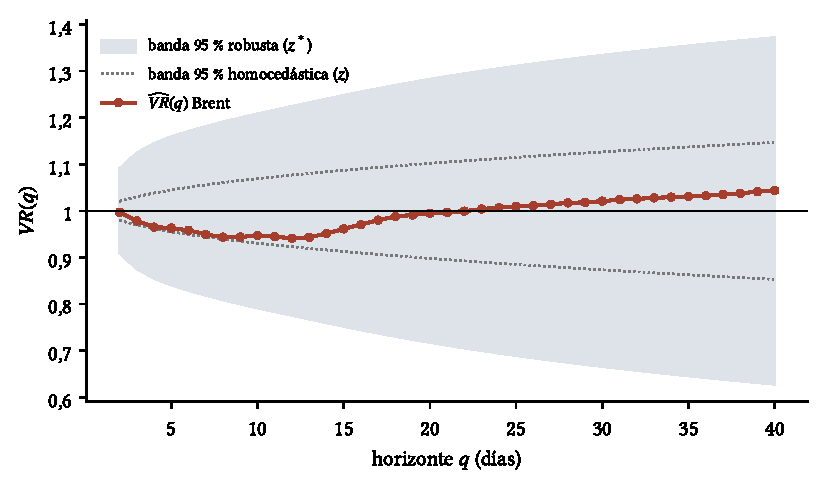
\includegraphics[width=0.72\linewidth]{graficos/cap07_ej01_vr_brent.pdf}
\caption{$\widehat{VR}(q)$ del Brent diario para $q=2,\dots,40$ con las bandas al 95\,\% bajo RW1 (punteada)
y robusta (sombreada). La razón se mantiene muy cerca de uno y siempre dentro de la banda robusta.}
\label{fig:vrbrent}
\end{figure}

\begin{conclusion}
No hay evidencia de que los rendimientos pasados del Brent predigan los futuros a horizontes de 2 a 40 días.
La forma débil de la eficiencia no se rechaza. La banda robusta es mucho más ancha que la homocedástica: usar
$z$ en lugar de $z^*$ hace parecer significativas desviaciones que son solo ruido.
\end{conclusion}
\end{ejresuelto}

\begin{ejresuelto}{Carteras pequeñas frente a grandes: el efecto adelanto-rezago}\label{ej:adelanto}
\enunciado Con las carteras mensuales formadas por tamaño y valor de la base de French (1949--2017), calcule
$\hat\rho_1$, $\widehat{VR}(q)$ y $z^*(q)$ para $q=2,4,12$. Luego calcule las correlaciones cruzadas entre la
cartera pequeña S1V3 y la grande S5V3, y estime la regresión
$r^P_t=a+b_1r^P_{t-1}+b_2r^G_{t-1}+e_t$. Interprete con la Proposición~\ref{prop:ajusteparcial}.

\solucion
\paso{Paso 1. Autocorrelación y tamaño.} Con $T=819$ meses:
\begin{center}\small
\begin{tabular}{@{}lrrrrrrr@{}}
\toprule
Cartera & $\hat\rho_1$ & $\widehat{VR}(2)$ & $z^*(2)$ & $\widehat{VR}(4)$ & $z^*(4)$ & $\widehat{VR}(12)$ & $z^*(12)$ \\
\midrule
S1V1 & 0,148 & 1,15 & 3,45 & 1,22 & 2,57 & 1,20 & 1,21 \\
S1V3 & 0,161 & 1,16 & 4,03 & 1,23 & 3,09 & 1,23 & 1,53 \\
S1V5 & 0,206 & 1,21 & 4,76 & 1,31 & 3,92 & 1,28 & 1,81 \\
S3V3 & 0,115 & 1,12 & 2,76 & 1,12 & 1,55 & 1,01 & 0,08 \\
S5V1 & 0,054 & 1,06 & 1,21 & 1,07 & 0,88 & 1,19 & 1,20 \\
S5V3 & 0,018 & 1,02 & 0,47 & 0,97 & $-0{,}33$ & 1,06 & 0,42 \\
S5V5 & 0,068 & 1,07 & 1,58 & 1,11 & 1,32 & 1,15 & 0,96 \\
\bottomrule
\end{tabular}
\end{center}
El patrón es nítido: las tres carteras pequeñas (S1) rechazan RW3 a $q=2$ y $q=4$; las grandes (S5), no. La
cartera mediana S3V3 queda en medio.

\paso{Paso 2. Comprobación de $VR(2)=1+\rho_1$.} Para S1V3, la Proposición~\ref{prop:vrrho} predice
\begin{align*}
  VR(2) &= 1+\hat\rho_1\\
        &= 1+0{,}161\\
        &= 1{,}161,
\end{align*}
que coincide con el $1{,}16$ estimado. Si los errores fueran homocedásticos, el estadístico sería
\begin{align*}
  z(2) &\approx \sqrt T\,\hat\rho_1\\
       &= \sqrt{819}\times0{,}161\\
       &= 28{,}62\times0{,}161\\
       &= 4{,}61,
\end{align*}
algo mayor que el robusto $z^*(2)=4{,}03$. El rechazo se mantiene con el robusto.

\paso{Paso 3. Correlaciones cruzadas.} Las correlaciones entre la pequeña en $t$ y la grande en $t-k$, y al
revés, son:
\begin{center}\small
\begin{tabular}{@{}rrr@{}}
\toprule
$k$ & $\operatorname{corr}(r^P_t,r^G_{t-k})$ & $\operatorname{corr}(r^G_t,r^P_{t-k})$ \\
\midrule
0 & 0,648 & 0,648 \\
1 & 0,155 & 0,027 \\
2 & $-0{,}005$ & $-0{,}062$ \\
3 & 0,056 & $-0{,}006$ \\
\bottomrule
\end{tabular}
\end{center}
En $k=1$ la asimetría es marcada: la grande del mes pasado se correlaciona $0{,}155$ con la pequeña de hoy, pero
la pequeña del mes pasado apenas $0{,}027$ con la grande de hoy. Es el patrón de la
Proposición~\ref{prop:ajusteparcial} (Figura~\ref{fig:adelanto}).

\paso{Paso 4. La regresión.} Por MCO:
\begin{align*}
  \hat r^P_t &= \underset{(0{,}0020)}{0{,}0092}+\underset{(0{,}0453)}{0{,}1045}\,r^P_{t-1}
               +\underset{(0{,}0624)}{0{,}1200}\,r^G_{t-1}.
\end{align*}
El coeficiente de la grande rezagada tiene $t=0{,}1200/0{,}0624=1{,}92$ ($p=0{,}055$), en el límite de la
significancia, y le quita parte del poder explicativo a la propia pequeña rezagada. Las dos variables están
muy correlacionadas (0,648), lo que infla los errores estándar.

\codigoweb{cap07_ej02}
\salidaR{cap07_ej02_R.txt}
\lectura{cap07_ej02}

\RvsPy El coeficiente de autocorrelación se calcula con la fórmula de la ACF muestral (desviaciones respecto de
la media de toda la muestra y denominador $\sum(x_t-\bar x)^2$), que es la que usa \texttt{acf()} de R.
\texttt{np.corrcoef(x[1:], x[:-1])} usa medias y varianzas distintas para cada submuestra y da un valor
ligeramente diferente; para las correlaciones cruzadas sí usamos \texttt{corrcoef} y \texttt{cor} en los dos
lenguajes, con idénticos resultados.

\begin{figure}[ht]
\centering
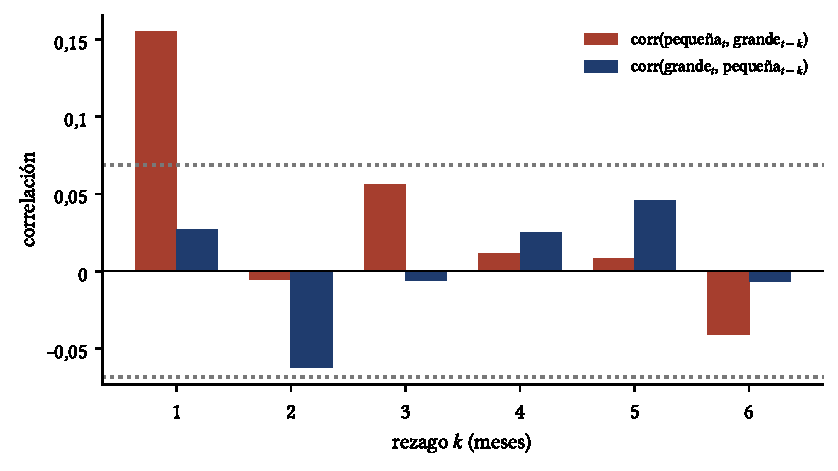
\includegraphics[width=0.72\linewidth]{graficos/cap07_ej02_adelanto_rezago.pdf}
\caption{Correlaciones cruzadas rezagadas entre la cartera pequeña S1V3 y la grande S5V3 (1949--2017). Las
líneas punteadas son la banda $\pm1{,}96/\sqrt T$. En el rezago 1 la grande adelanta a la pequeña, pero no al
revés.}
\label{fig:adelanto}
\end{figure}

\begin{conclusion}
Las carteras de empresas pequeñas violan RW3 a horizontes mensuales cortos, y su predictibilidad viene en
buena parte del mercado de las grandes. El patrón es el que produce el ajuste parcial de precios. No implica
por sí mismo una ganancia explotable, porque las acciones pequeñas son las más caras de negociar.
\end{conclusion}
\end{ejresuelto}

\begin{ejresuelto}{¿Revierten a la media las acciones en horizontes de años?}\label{ej:reversion}
\enunciado Con la base de Shiller, construya el rendimiento real total anual del S\&P 500 (enero a enero,
1871--2023), incluyendo dividendos y descontando la inflación. Calcule $\widehat{VR}(q)$, $z$ y $z^*$ para
$q=2,3,5,8,10$ años. ¿Hay evidencia de reversión a la media? ¿Qué tan concluyente es?

\solucion
\paso{Paso 1. Construcción del rendimiento.} Con $P_t$ el índice, $D_t$ el dividendo anualizado y $I_t$ el
IPC mensual, el rendimiento real total del mes $t$ es
\begin{align*}
  g_t &= \ln\Bigl(\frac{P_t+D_t/12}{P_{t-1}}\Bigr)-\ln\Bigl(\frac{I_t}{I_{t-1}}\Bigr).
\end{align*}
Acumulamos $g_t$ en un índice de riqueza real en logaritmos y tomamos la diferencia entre eneros consecutivos.
Resultan $T=152$ rendimientos anuales, con media $0{,}0664$ (6,6\,\% real), desviación estándar $0{,}1725$ y
$\hat\rho_1=0{,}013$.

\paso{Paso 2. Las razones de varianzas.}
\begin{center}\small
\begin{tabular}{@{}rrrr@{}}
\toprule
$q$ (años) & $\widehat{VR}(q)$ & $z$ & $z^*$ \\
\midrule
2  & 1,019 & 0,23 & 0,21 \\
3  & 0,907 & $-0{,}77$ & $-0{,}71$ \\
5  & 0,886 & $-0{,}64$ & $-0{,}60$ \\
8  & 0,841 & $-0{,}66$ & $-0{,}61$ \\
10 & 0,828 & $-0{,}63$ & $-0{,}58$ \\
\bottomrule
\end{tabular}
\end{center}
A partir de $q=3$ la razón cae por debajo de uno y sigue bajando con el horizonte: la forma que predice la
Proposición~\ref{prop:poterba}. A 10 años la varianza es un 17\,\% menor que la que implicaría un paseo
aleatorio.

\paso{Paso 3. La significancia.} Para $q=10$, la desviación estándar bajo RW1 es $0{,}274$ (calculada en la
sección de reversión a la media), y
\begin{align*}
  z(10) &= \frac{0{,}828-1}{0{,}2739}\\
        &= \frac{-0{,}172}{0{,}2739}\\
        &= -0{,}63 .
\end{align*}
Ningún estadístico se acerca a $-1{,}96$. Con 152 años, una prueba al 5\,\% a dos colas solo rechazaría con
$\widehat{VR}(10)<1-1{,}96\times0{,}274=0{,}46$.

\codigoweb{cap07_ej03}
\salidaR{cap07_ej03_R.txt}
\lectura{cap07_ej03}

\RvsPy La base de Shiller tiene dividendos solo hasta junio de 2023, así que cortamos la muestra ahí en los dos
lenguajes. En R el nombre de la columna \texttt{Consumer Price Index} se convierte en
\texttt{Consumer.Price.Index} al leer el archivo; en \texttt{pandas} conserva los espacios.

\begin{figure}[ht]
\centering
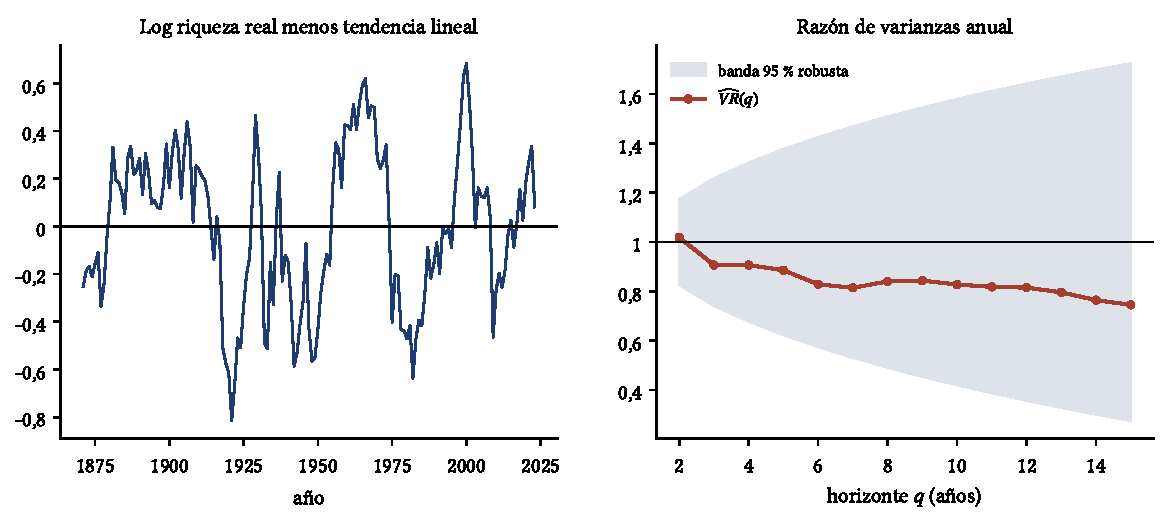
\includegraphics[width=\linewidth]{graficos/cap07_ej03_reversion.pdf}
\caption{Izquierda: logaritmo de la riqueza real del S\&P 500 (enero de cada año) menos su tendencia lineal; las
desviaciones de varias décadas sugieren un componente transitorio. Derecha: $\widehat{VR}(q)$ anual con la
banda robusta al 95\,\%: la razón desciende con el horizonte, pero la banda es tan ancha que no se puede
rechazar el paseo aleatorio.}
\label{fig:reversion}
\end{figure}

\begin{conclusion}
Los rendimientos reales de largo plazo del S\&P 500 muestran el patrón de la reversión a la media, pero la
evidencia estadística es débil. Con un siglo y medio de datos hay muy pocas observaciones independientes de
horizonte largo; ``no rechazar'' aquí significa sobre todo ``no se puede saber con estos datos''.
\end{conclusion}
\end{ejresuelto}

\begin{ejresuelto}{Prueba de rachas sobre los signos}\label{ej:rachas}
\enunciado Aplique la prueba de rachas a los signos de los rendimientos diarios del Brent y de los rendimientos
mensuales de las carteras S1V3 y S5V3. Excluya los rendimientos exactamente iguales a cero. Compare con los
resultados de la razón de varianzas.

\solucion
\paso{Paso 1. Conteo.} En el Brent hay 171 días con rendimiento cero, que se excluyen; quedan $n_1=4\,617$ días
de subida y $n_2=4\,333$ de bajada, $n=8\,950$, y se observan $R=4\,395$ rachas.

\paso{Paso 2. Media y varianza bajo independencia.} Primero
\begin{align*}
  2n_1n_2 &= 2\times4\,617\times4\,333\\
          &= 40\,010\,922 .
\end{align*}
Entonces
\begin{align*}
  \E[R] &= \frac{40\,010\,922}{8\,950}+1\\
        &= 4\,470{,}49+1\\
        &= 4\,471{,}49,\\[4pt]
  \Var[R] &= \frac{40\,010\,922\,(40\,010\,922-8\,950)}{8\,950^2\,(8\,950-1)}\\
          &= 2\,232{,}75,\\[4pt]
  \sqrt{\Var[R]} &= 47{,}25 .
\end{align*}

\paso{Paso 3. Estadístico.}
\begin{align*}
  Z &= \frac{4\,395-4\,471{,}49}{47{,}25}\\
    &= \frac{-76{,}49}{47{,}25}\\
    &= -1{,}62 .
\end{align*}
No se rechaza la aleatoriedad de los signos al 5\,\%.

\paso{Paso 4. Las carteras.} Con los mismos pasos:
\begin{center}\small
\begin{tabular}{@{}lrrrrr@{}}
\toprule
Serie & $n_1$ & $n_2$ & $R$ & $\E[R]$ & $Z$ \\
\midrule
Brent diario & 4\,617 & 4\,333 & 4\,395 & 4\,471,5 & $-1{,}62$ \\
S1V3 mensual & 494 & 325 & 343 & 393,1 & $-3{,}66$ \\
S5V3 mensual & 511 & 308 & 383 & 385,3 & $-0{,}17$ \\
\bottomrule
\end{tabular}
\end{center}
Para S1V3, $Z=(343-393{,}06)/13{,}69=-3{,}66$: hay unas 50 rachas menos de las esperadas, es decir, los meses
buenos y malos de las acciones pequeñas tienden a agruparse. Es la misma persistencia que detectó la razón de
varianzas ($z^*(2)=4{,}03$). Para S5V3 no hay nada.

\codigoweb{cap07_ej04}
\salidaR{cap07_ej04_R.txt}
\lectura{cap07_ej04}

\RvsPy Python comprueba el cálculo con \texttt{runstest\_1samp} de \texttt{statsmodels}, que corta en
\texttt{cutoff=0.5} la serie de ceros y unos. Por defecto aplica una corrección de continuidad para muestras
pequeñas; la desactivamos (\texttt{correction=False}) para reproducir la fórmula de la
Proposición~\ref{prop:rachas}.

\begin{figure}[ht]
\centering
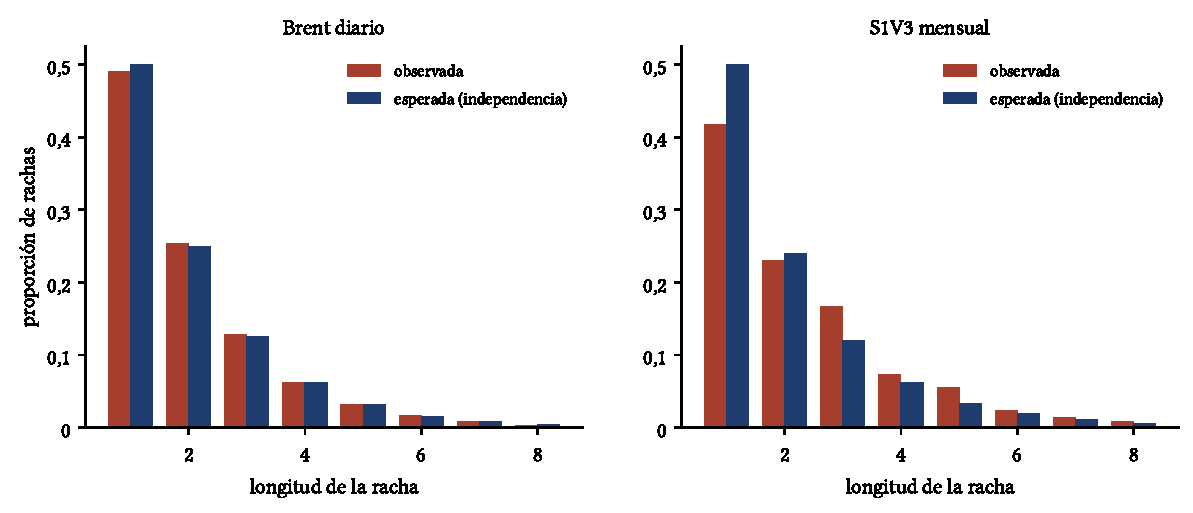
\includegraphics[width=\linewidth]{graficos/cap07_ej04_rachas.pdf}
\caption{Distribución de la longitud de las rachas observadas frente a la esperada si los signos fueran
independientes (distribución geométrica). En el Brent las barras casi coinciden; en la cartera pequeña S1V3 hay
menos rachas de longitud 1 y más rachas largas que las esperadas.}
\label{fig:rachas}
\end{figure}

\begin{conclusion}
La prueba de rachas, que solo mira los signos, confirma lo que mostró la razón de varianzas: el Brent diario y
las acciones grandes son compatibles con un paseo aleatorio, mientras que los rendimientos de las acciones
pequeñas persisten. Que dos pruebas de naturaleza distinta coincidan da más confianza en el resultado.
\end{conclusion}
\end{ejresuelto}

\begin{ejresuelto}{El factor momentum: rentabilidad y desplomes}\label{ej:momentum}
\enunciado Con el factor UMD mensual de French (1949--2017), calcule su rendimiento medio anualizado, su
volatilidad, su razón de Sharpe y su asimetría; contraste que la media es cero con errores estándar clásicos y de
Newey-West; identifique el peor mes y la máxima caída acumulada; y compare las submuestras 1949--1999 y
2000--2017.

\solucion
\paso{Paso 1. Momentos.} Con $T=819$ meses, la media mensual es $0{,}0070$ (8,37\,\% anual) y la desviación
estándar anual es 13,49\,\%, de modo que la mensual es $13{,}49/\sqrt{12}=3{,}89$\,\%. La razón de Sharpe anual
es
\begin{align*}
  SR &= \frac{\sqrt{12}\,\bar m}{s}\\
     &= \frac{8{,}37}{13{,}49}\\
     &= 0{,}620 .
\end{align*}
Como UMD es una cartera de costo cero (larga en ganadoras y corta en perdedoras), su media es directamente un
exceso de rendimiento. La asimetría es $-1{,}378$: las pérdidas extremas son más grandes que las ganancias
extremas.

\paso{Paso 2. Significancia.} El estadístico $t$ clásico es $5{,}13$. Con Newey-West y
$L=\lfloor4(819/100)^{2/9}\rfloor=6$ rezagos, $t=5{,}06$. La autocorrelación de UMD es pequeña, así que la
corrección casi no cambia nada, y la media es claramente distinta de cero.

\paso{Paso 3. El riesgo de cola.} El peor mes fue abril de 2009, con $-34{,}58$\,\%, en plena recuperación del
mercado tras la crisis financiera: las perdedoras de 2008 (bancos, empresas cíclicas) subieron con fuerza y la
posición corta las sufrió. La caída acumulada máxima desde un máximo fue de $-57{,}6$\,\%, con el fondo en
septiembre de 2009 (Figura~\ref{fig:momentum}).

\paso{Paso 4. Submuestras.}
\begin{center}\small
\begin{tabular}{@{}lrr@{}}
\toprule
Período & Media anual & $t$ \\
\midrule
1949--1999 & 10,64\,\% & 7,01 \\
2000--2017 & 1,67\,\% & 0,36 \\
\bottomrule
\end{tabular}
\end{center}
Después de 2000, ya publicado el trabajo de Jegadeesh y Titman (1993), el rendimiento medio cae a menos de la
sexta parte y deja de ser significativo.

\codigoweb{cap07_ej05}
\salidaR{cap07_ej05_R.txt}
\lectura{cap07_ej05}

\RvsPy En R programamos la varianza de Newey-West con los pesos de Bartlett $1-j/(L+1)$; en Python la obtenemos
regresando UMD sobre una constante con \texttt{cov\_type="HAC"}, y los dos dan $t=5{,}06$. La caída acumulada
usa \texttt{cummax} en R y \texttt{np.maximum.accumulate} en Python.

\begin{figure}[ht]
\centering
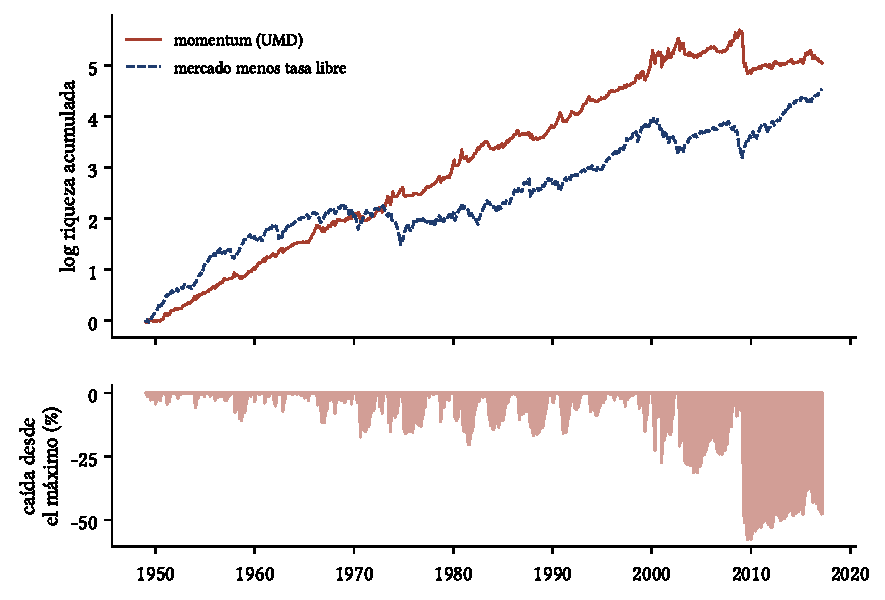
\includegraphics[width=0.78\linewidth]{graficos/cap07_ej05_momentum.pdf}
\caption{Arriba: logaritmo de la riqueza acumulada del factor momentum y del exceso de rendimiento del mercado
(1949--2017). Abajo: caída del momentum desde su máximo previo; el desplome de 2009 devuelve la riqueza
acumulada al nivel de 1999 y borra casi una década de ganancias.}
\label{fig:momentum}
\end{figure}

\begin{conclusion}
El momentum es la anomalía de forma débil más robusta del siglo XX: una estrategia basada solo en precios pasados
obtuvo un exceso de rendimiento de 8,4\,\% anual con $t>5$. Pero tiene una cola izquierda pesada, y su
rendimiento cayó drásticamente tras su publicación. Ambas observaciones son compatibles con una prima por riesgo
de desplome, con el aprendizaje de los inversionistas o con ambas cosas: el problema de la hipótesis conjunta
impide decidirlo con estos datos.
\end{conclusion}
\end{ejresuelto}

% ---------------------------------------------------------------------
\section{Ejercicios propuestos}
% ---------------------------------------------------------------------

\begin{enumerate}[label=\textbf{\thechapter.\arabic*},leftmargin=*,itemsep=6pt]
  \item Demuestre directamente, sin usar la Proposición~\ref{prop:vrrho}, que
  $\Var(r_t+r_{t-1})=2\sigma^2(1+\rho_1)$ y concluya que $VR(2)=1+\rho_1$.

  \item Para rendimientos AR(1) con $\rho=-0{,}2$, calcule $VR(4)$ con la Proposición~\ref{prop:vrrho} y el
  límite cuando $q\to\infty$. \textit{Respuesta: $VR(4)=0{,}736$; límite $0{,}667$.}

  \item Calcule la desviación estándar asintótica de $\widehat{VR}(12)$ bajo RW1 con $T=819$. ¿Desde qué valor
  de $\widehat{VR}(12)$ rechazaría RW1 al 5\,\%? \textit{Respuesta: $0{,}131$; fuera de $1\pm0{,}257$.}

  \item En el modelo de Poterba y Summers con $\sigma_w^2=1$, $\phi=0{,}9$ y $\gamma_0=5$, calcule $VR(10)$ y el
  límite. \textit{Respuesta: $VR(10)=0{,}826$; límite $0{,}5$.}

  \item Con $n_1=n_2=50$, calcule $\E[R]$ y $\Var[R]$ en la prueba de rachas. ¿Cuántas rachas o menos llevarían a
  rechazar la independencia al 5\,\% a dos colas? \textit{Respuesta: $51$ y $24{,}75$; $R\le41$.}

  \item En el modelo de ajuste parcial con $a=0{,}7$, calcule la correlación entre $r^P_t$ y $r^G_{t-1}$.
  ¿Para qué valor de $a$ es máxima la autocorrelación de $r^P_t$? \textit{Respuesta: $0{,}394$; $a=1/2$, con
  $\rho_1=1/2$.}

  \item \emph{(Con datos del BCRP.)} Descargue el tipo de cambio interbancario diario sol/dólar y calcule
  $\widehat{VR}(q)$ y $z^*(q)$ para $q=2,5,10,20$. Repita para el índice S\&P/BVL Perú General. ¿Cuál de los dos
  mercados se parece más a un paseo aleatorio? ¿Qué papel cree que juegan las intervenciones cambiarias del BCRP?

  \item \emph{(Simulación.)} Repita la simulación de la Figura~\ref{fig:vrtamano} con $T=250$ y con
  innovaciones $t$ de Student con 5 grados de libertad. ¿Empeora el tamaño de $z$? ¿Y el de $z^*$?

  \item \emph{(Con datos.)} Divida la muestra de la cartera S1V3 en 1949--1982 y 1983--2017 y repita el
  Ejercicio~\ref{ej:adelanto}. ¿Se ha reducido la predictibilidad de las acciones pequeñas a medida que el
  mercado se volvió más líquido?
\end{enumerate}

% ---------------------------------------------------------------------
\section{Resumen de fórmulas}
% ---------------------------------------------------------------------

\begin{table}[H]
\centering\small
\begin{tabular}{@{}ll@{}}
\toprule
Concepto & Fórmula \\
\midrule
Razón de varianzas & $VR(q)=1+2\sum_{j=1}^{q-1}(1-j/q)\rho_j$;\quad $VR(2)=1+\rho_1$ \\
Rendimientos AR(1) & $\lim_{q\to\infty}VR(q)=(1+\rho)/(1-\rho)$ \\
Prueba bajo RW1 & $z=(\widehat{VR}-1)/\sqrt{2(2q-1)(q-1)/(3qT)}$ \\
Prueba robusta & $z^*=(\widehat{VR}-1)/\sqrt{\hat\theta/T}$;\quad $\hat\theta=\sum_j[2(q-j)/q]^2\hat\delta_j$ \\
Poterba-Summers & $\lim_{k\to\infty}VR(k)=\sigma_w^2/[\sigma_w^2+2\gamma_0(1-\phi)]$ \\
Rachas & $\E[R]=2n_1n_2/n+1$;\quad $\Var[R]=2n_1n_2(2n_1n_2-n)/[n^2(n-1)]$ \\
Ajuste parcial & $\rho_1=a(1-a)/[a^2+(1-a)^2]$ \\
Razón de Sharpe anual & $SR=\sqrt{12}\,\bar m/s$ (datos mensuales) \\
\bottomrule
\end{tabular}
\caption{Fórmulas principales del Capítulo 7.}
\end{table}

\section*{Referencias}
\begin{itemize}[leftmargin=*]
  \item Campbell, J. Y., Lo, A. W. y MacKinlay, A. C. (1997). \emph{The Econometrics of Financial Markets}.
        Princeton University Press. Capítulo 2.
  \item Chow, K. V. y Denning, K. C. (1993). A simple multiple variance ratio test. \emph{Journal of
        Econometrics}, 58(3), 385--401.
  \item Daniel, K. y Moskowitz, T. J. (2016). Momentum crashes. \emph{Journal of Financial Economics}, 122(2),
        221--247.
  \item Fama, E. F. (1970). Efficient capital markets: A review of theory and empirical work. \emph{Journal of
        Finance}, 25(2), 383--417.
  \item Fama, E. F. y French, K. R. (1988). Permanent and temporary components of stock prices. \emph{Journal
        of Political Economy}, 96(2), 246--273.
  \item Jegadeesh, N. y Titman, S. (1993). Returns to buying winners and selling losers: Implications for stock
        market efficiency. \emph{Journal of Finance}, 48(1), 65--91.
  \item Kim, J. H. (2006). Wild bootstrapping variance ratio tests. \emph{Economics Letters}, 92(1), 38--43.
  \item Lo, A. W. y MacKinlay, A. C. (1988). Stock market prices do not follow random walks: Evidence from a
        simple specification test. \emph{Review of Financial Studies}, 1(1), 41--66.
  \item Lo, A. W. y MacKinlay, A. C. (1990). When are contrarian profits due to stock market overreaction?
        \emph{Review of Financial Studies}, 3(2), 175--205.
  \item McLean, R. D. y Pontiff, J. (2016). Does academic research destroy stock return predictability?
        \emph{Journal of Finance}, 71(1), 5--32.
  \item Poterba, J. M. y Summers, L. H. (1988). Mean reversion in stock prices: Evidence and implications.
        \emph{Journal of Financial Economics}, 22(1), 27--59.
  \item Richardson, M. y Stock, J. H. (1989). Drawing inferences from statistics based on multiyear asset
        returns. \emph{Journal of Financial Economics}, 25(2), 323--348.
  \item Wald, A. y Wolfowitz, J. (1940). On a test whether two samples are from the same population.
        \emph{Annals of Mathematical Statistics}, 11(2), 147--162.
\end{itemize}

% =====================================================================
%  Capítulo 8. Modelos ARCH y GARCH
% =====================================================================
\part{Volatilidad}
\chapter[Modelos ARCH y GARCH]{Volatilidad condicional: modelos ARCH y GARCH}\label{cap:garch}

\section*{Objetivos de aprendizaje}
Al terminar este capítulo, el lector podrá:
\begin{enumerate}[label=\arabic*.,leftmargin=*]
  \item Derivar los momentos de los procesos ARCH(1) y GARCH(1,1), en particular su varianza incondicional y
        su curtosis, y explicar por qué generan colas gruesas y agrupamiento de volatilidad.
  \item Detectar efectos ARCH con la prueba de Ljung-Box sobre los cuadrados y la prueba LM de Engle.
  \item Programar y maximizar la verosimilitud de un GARCH(1,1) con innovaciones normales y $t$ de Student, y
        calcular errores estándar robustos de cuasi máxima verosimilitud.
  \item Pronosticar la varianza a varios horizontes, calcular la vida media de los choques y evaluar los
        pronósticos fuera de muestra con funciones de pérdida apropiadas.
\end{enumerate}

\section*{Motivación}
El Capítulo~\ref{cap:hechos} mostró que los rendimientos casi no están autocorrelacionados, pero sus cuadrados
sí: los días agitados vienen juntos y los tranquilos también. El Capítulo~\ref{cap:robustos} trató esa
heterocedasticidad como un estorbo para la inferencia; el Capítulo~\ref{cap:eficiencia}, como una razón para
usar pruebas robustas. Este capítulo la convierte en el objeto de estudio. La volatilidad no se observa, pero
es predecible, y su pronóstico es la materia prima de la gestión de riesgos (valor en riesgo, Capítulo~13), de
la valoración de opciones y de la asignación de carteras. Engle (1982) propuso el modelo ARCH para la inflación
británica; Bollerslev (1986) lo generalizó al GARCH, que sigue siendo el modelo de referencia.

\paragraph{Datos del capítulo.} Rendimientos logarítmicos diarios del Brent en porcentaje (mayo de 1987 a
noviembre de 2026, $T=9\,121$) y rendimientos mensuales del S\&P 500 (base de Shiller, 1871--2026). Expresar
los rendimientos en porcentaje (multiplicar por 100) no cambia nada sustantivo, pero evita que $\omega$ sea un
número del orden de $10^{-6}$, lo que dificulta la optimización numérica.

% ---------------------------------------------------------------------
\section{El modelo ARCH}
% ---------------------------------------------------------------------

Escribimos el rendimiento como su media condicional más una innovación,
\[
  r_t=\mu+\varepsilon_t,\qquad \varepsilon_t=\sigma_t z_t,\qquad z_t\sim\text{i.i.d.}(0,1),
\]
donde $\sigma_t$ depende solo de la información hasta $t-1$. Entonces
$\E[\varepsilon_t\mid\mathcal F_{t-1}]=\sigma_t\E[z_t]=0$ y
$\Var(\varepsilon_t\mid\mathcal F_{t-1})=\sigma_t^2\E[z_t^2]=\sigma_t^2$: $\sigma_t^2$ es la \emph{varianza
condicional}.

\begin{definicion}[ARCH($q$); Engle, 1982]
La innovación sigue un proceso autorregresivo condicionalmente heterocedástico de orden $q$ si
\[
  \sigma_t^2=\omega+\alpha_1\varepsilon_{t-1}^2+\dots+\alpha_q\varepsilon_{t-q}^2,
  \qquad \omega>0,\ \alpha_i\ge0 .
\]
\end{definicion}

Un rendimiento grande hoy, de cualquier signo, eleva la varianza de mañana; eso produce agrupamiento de
volatilidad. Las restricciones de signo garantizan que $\sigma_t^2>0$.

\begin{proposicion}[Propiedades del ARCH(1)]\label{prop:arch1}
Sea $\sigma_t^2=\omega+\alpha\varepsilon_{t-1}^2$ con $z_t\sim N(0,1)$ y $0\le\alpha<1$. Entonces:
\begin{enumerate}[label=(\roman*)]
  \item $\varepsilon_t$ no está autocorrelacionado;
  \item su varianza incondicional es $\sigma^2=\omega/(1-\alpha)$;
  \item $\varepsilon_t^2$ sigue un AR(1): $\varepsilon_t^2=\omega+\alpha\varepsilon_{t-1}^2+v_t$, con
        $\E[v_t\mid\mathcal F_{t-1}]=0$;
  \item si $3\alpha^2<1$, la curtosis es $\kappa=3(1-\alpha^2)/(1-3\alpha^2)>3$.
\end{enumerate}
\end{proposicion}

\begin{proof}
(i) Como $\E[\varepsilon_t\mid\mathcal F_{t-1}]=0$, la Proposición~\ref{prop:martingala} con $g=\varepsilon_{t-j}$
da $\Cov(\varepsilon_t,\varepsilon_{t-j})=0$ para $j\ge1$.

(ii) Por la ley de esperanzas iteradas, y usando la estacionariedad ($\E[\varepsilon_t^2]=\E[\varepsilon_{t-1}^2]=\sigma^2$):
\begin{align*}
  \E[\varepsilon_t^2] &= \E\bigl[\E[\sigma_t^2z_t^2\mid\mathcal F_{t-1}]\bigr]\\
                      &= \E[\sigma_t^2]\\
                      &= \omega+\alpha\,\E[\varepsilon_{t-1}^2],\\[4pt]
  \sigma^2            &= \omega+\alpha\,\sigma^2,\\
  \sigma^2(1-\alpha)  &= \omega,\\
  \sigma^2            &= \frac{\omega}{1-\alpha}.
\end{align*}

(iii) Definimos $v_t=\varepsilon_t^2-\sigma_t^2$. Entonces
\begin{align*}
  \varepsilon_t^2 &= \sigma_t^2+v_t\\
                  &= \omega+\alpha\varepsilon_{t-1}^2+v_t,\\[4pt]
  \E[v_t\mid\mathcal F_{t-1}] &= \E[\varepsilon_t^2\mid\mathcal F_{t-1}]-\sigma_t^2\\
                              &= \sigma_t^2-\sigma_t^2\\
                              &= 0 .
\end{align*}

(iv) Con $z_t$ normal, $\E[z_t^4]=3$. Sea $m_4=\E[\varepsilon_t^4]$, igual para todo $t$ por estacionariedad:
\begin{align*}
  m_4 &= \E[\sigma_t^4z_t^4]\\
      &= 3\,\E[\sigma_t^4]\\
      &= 3\,\E\bigl[(\omega+\alpha\varepsilon_{t-1}^2)^2\bigr]\\
      &= 3\bigl(\omega^2+2\omega\alpha\,\E[\varepsilon_{t-1}^2]+\alpha^2\E[\varepsilon_{t-1}^4]\bigr)\\
      &= 3\omega^2+6\omega\alpha\sigma^2+3\alpha^2m_4 .
\end{align*}
Despejamos $m_4$ y usamos $\omega=\sigma^2(1-\alpha)$:
\begin{align*}
  m_4(1-3\alpha^2) &= 3\omega^2+6\omega\alpha\sigma^2\\
                   &= 3\omega(\omega+2\alpha\sigma^2)\\
                   &= 3\sigma^2(1-\alpha)\bigl[\sigma^2(1-\alpha)+2\alpha\sigma^2\bigr]\\
                   &= 3\sigma^4(1-\alpha)(1+\alpha)\\
                   &= 3\sigma^4(1-\alpha^2).
\end{align*}
Dividiendo entre $\sigma^4(1-3\alpha^2)$, que es positivo si $3\alpha^2<1$:
\begin{align*}
  \kappa &= \frac{m_4}{\sigma^4}\\
         &= \frac{3(1-\alpha^2)}{1-3\alpha^2}.
\end{align*}
Como $1-\alpha^2>1-3\alpha^2$ cuando $\alpha>0$, el cociente es mayor que uno y $\kappa>3$.
\end{proof}

La parte (iv) es notable: aunque cada $z_t$ es normal, la distribución \emph{incondicional} de $\varepsilon_t$
tiene colas más gruesas que la normal, porque es una mezcla de normales con varianzas distintas. Con
$\omega=0{,}5$ y $\alpha=0{,}5$ la varianza incondicional es $0{,}5/0{,}5=1$ y
\begin{align*}
  \kappa &= \frac{3(1-0{,}25)}{1-0{,}75}\\
         &= \frac{2{,}25}{0{,}25}\\
         &= 9 .
\end{align*}
La Figura~\ref{fig:archsim} compara una trayectoria de ese proceso con ruido normal de la misma varianza: el
ARCH alterna tramos tranquilos y ráfagas de valores extremos, y su densidad (estimada con 400\,000
simulaciones, cuya curtosis muestral es $9{,}67$) tiene más pico y colas mucho más altas que la normal.

\begin{figure}[ht]
\centering
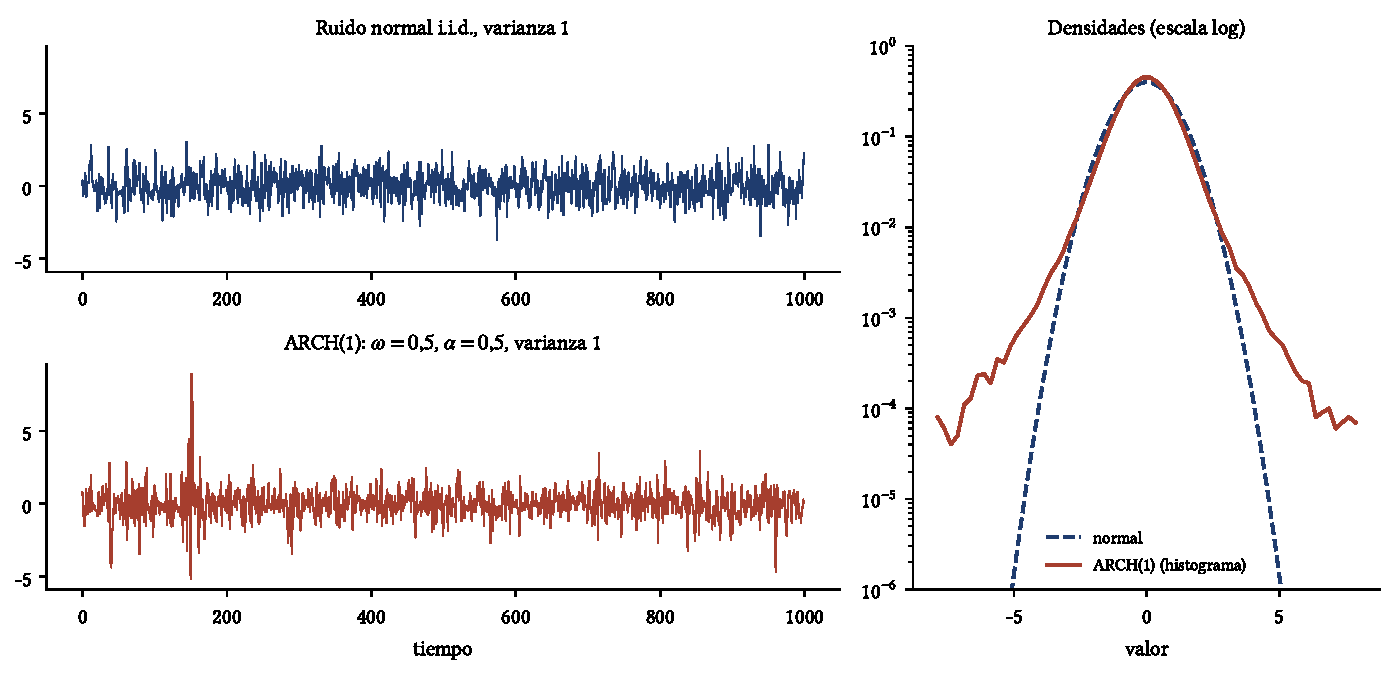
\includegraphics[width=\linewidth]{graficos/cap08_fig_arch_sim.pdf}
\caption{Izquierda: ruido normal i.i.d.\ y un ARCH(1) con $\omega=\alpha=0{,}5$, ambos con varianza
incondicional 1. Derecha: densidad del ARCH(1) frente a la normal en escala logarítmica; las colas del ARCH
caen mucho más despacio.}
\label{fig:archsim}
\end{figure}

% ---------------------------------------------------------------------
\section{El modelo GARCH}
% ---------------------------------------------------------------------

En la práctica, un ARCH necesita muchos rezagos para reproducir la persistencia de la volatilidad. Bollerslev
(1986) agregó la varianza rezagada a la ecuación.

\begin{definicion}[GARCH(1,1)]
\[
  \sigma_t^2=\omega+\alpha\,\varepsilon_{t-1}^2+\beta\,\sigma_{t-1}^2,\qquad
  \omega>0,\ \alpha\ge0,\ \beta\ge0 .
\]
\end{definicion}

La varianza de mañana es un promedio ponderado de un nivel de largo plazo, la ``noticia'' de hoy
($\varepsilon_{t-1}^2$) y la varianza de hoy. El coeficiente $\alpha$ mide la reacción a las noticias y
$\beta$ la inercia.

\begin{proposicion}[Representación ARCH($\infty$)]\label{prop:archinf}
Si $0\le\beta<1$,
\[
  \sigma_t^2=\frac{\omega}{1-\beta}+\alpha\sum_{j=1}^{\infty}\beta^{\,j-1}\varepsilon_{t-j}^2 .
\]
\end{proposicion}

\begin{proof}
Sustituimos la ecuación del GARCH en sí misma para $\sigma_{t-1}^2$, luego para $\sigma_{t-2}^2$, y así
sucesivamente:
\begin{align*}
  \sigma_t^2 &= \omega+\alpha\varepsilon_{t-1}^2+\beta\sigma_{t-1}^2\\
             &= \omega+\alpha\varepsilon_{t-1}^2+\beta\bigl(\omega+\alpha\varepsilon_{t-2}^2+\beta\sigma_{t-2}^2\bigr)\\
             &= \omega(1+\beta)+\alpha\bigl(\varepsilon_{t-1}^2+\beta\varepsilon_{t-2}^2\bigr)+\beta^2\sigma_{t-2}^2\\
             &\;\;\vdots\\
             &= \omega\sum_{j=0}^{k-1}\beta^j+\alpha\sum_{j=1}^{k}\beta^{\,j-1}\varepsilon_{t-j}^2+\beta^k\sigma_{t-k}^2 .
\end{align*}
Cuando $k\to\infty$, $\beta^k\sigma_{t-k}^2\to0$ y la serie geométrica converge:
\begin{align*}
  \omega\sum_{j=0}^{\infty}\beta^j &= \frac{\omega}{1-\beta}. && \qedhere
\end{align*}
\end{proof}

El GARCH(1,1) es entonces un ARCH de orden infinito con pesos que decrecen geométricamente: con solo tres
parámetros recuerda todo el pasado.

\begin{proposicion}[Momentos del GARCH(1,1)]\label{prop:garchmom}
Si $\alpha+\beta<1$:
\begin{enumerate}[label=(\roman*)]
  \item la varianza incondicional es $\bar\sigma^2=\omega/(1-\alpha-\beta)$;
  \item $\varepsilon_t^2$ sigue un ARMA(1,1):
        $\varepsilon_t^2=\omega+(\alpha+\beta)\varepsilon_{t-1}^2+v_t-\beta v_{t-1}$, con
        $v_t=\varepsilon_t^2-\sigma_t^2$;
  \item con $z_t$ normal y $(\alpha+\beta)^2+2\alpha^2<1$, la curtosis es
        \[
          \kappa=\frac{3\bigl[1-(\alpha+\beta)^2\bigr]}{1-(\alpha+\beta)^2-2\alpha^2}>3 .
        \]
\end{enumerate}
\end{proposicion}

\begin{proof}
(i) Tomamos esperanzas en la ecuación del GARCH, con $\E[\varepsilon_{t-1}^2]=\E[\sigma_{t-1}^2]=\bar\sigma^2$:
\begin{align*}
  \bar\sigma^2 &= \omega+\alpha\bar\sigma^2+\beta\bar\sigma^2,\\
  \bar\sigma^2(1-\alpha-\beta) &= \omega,\\
  \bar\sigma^2 &= \frac{\omega}{1-\alpha-\beta}.
\end{align*}

(ii) Sustituimos $\sigma_t^2=\varepsilon_t^2-v_t$ y $\sigma_{t-1}^2=\varepsilon_{t-1}^2-v_{t-1}$:
\begin{align*}
  \varepsilon_t^2-v_t &= \omega+\alpha\varepsilon_{t-1}^2+\beta\bigl(\varepsilon_{t-1}^2-v_{t-1}\bigr),\\
  \varepsilon_t^2     &= \omega+(\alpha+\beta)\varepsilon_{t-1}^2+v_t-\beta v_{t-1}.
\end{align*}

(iii) Escribimos la recursión en función de $z_{t-1}$, usando $\varepsilon_{t-1}^2=\sigma_{t-1}^2z_{t-1}^2$:
\begin{align*}
  \sigma_t^2 &= \omega+\sigma_{t-1}^2\bigl(\alpha z_{t-1}^2+\beta\bigr).
\end{align*}
Como $z_{t-1}$ es independiente de $\sigma_{t-1}^2$, con $\E[z^2]=1$ y $\E[z^4]=3$:
\begin{align*}
  \E\bigl[(\alpha z^2+\beta)^2\bigr] &= \alpha^2\E[z^4]+2\alpha\beta\E[z^2]+\beta^2\\
                                     &= 3\alpha^2+2\alpha\beta+\beta^2\\
                                     &= (\alpha+\beta)^2+2\alpha^2 .
\end{align*}
Llamamos $c=(\alpha+\beta)^2+2\alpha^2$ y $m=\E[\sigma_t^4]$. Elevamos al cuadrado y tomamos esperanzas:
\begin{align*}
  m &= \omega^2+2\omega\,\E[\sigma_{t-1}^2]\,\E[\alpha z^2+\beta]+\E[\sigma_{t-1}^4]\,\E\bigl[(\alpha z^2+\beta)^2\bigr]\\
    &= \omega^2+2\omega\bar\sigma^2(\alpha+\beta)+c\,m,\\[4pt]
  m(1-c) &= \omega^2+2\omega\bar\sigma^2(\alpha+\beta).
\end{align*}
Con $\omega=\bar\sigma^2(1-\alpha-\beta)$, el lado derecho es
\begin{align*}
  \omega\bigl[\omega+2\bar\sigma^2(\alpha+\beta)\bigr]
    &= \bar\sigma^2(1-\alpha-\beta)\,\bar\sigma^2\bigl[(1-\alpha-\beta)+2(\alpha+\beta)\bigr]\\
    &= \bar\sigma^4(1-\alpha-\beta)(1+\alpha+\beta)\\
    &= \bar\sigma^4\bigl[1-(\alpha+\beta)^2\bigr].
\end{align*}
Finalmente, $\E[\varepsilon_t^4]=\E[\sigma_t^4]\E[z_t^4]=3m$, y si $c<1$:
\begin{align*}
  \kappa &= \frac{3m}{\bar\sigma^4}\\
         &= \frac{3\bigl[1-(\alpha+\beta)^2\bigr]}{1-c}\\
         &= \frac{3\bigl[1-(\alpha+\beta)^2\bigr]}{1-(\alpha+\beta)^2-2\alpha^2}.
\end{align*}
El denominador es menor que el término entre corchetes cuando $\alpha>0$, así que $\kappa>3$.
\end{proof}

La parte (ii) explica la forma de la ACF de los cuadrados: decae geométricamente a la tasa $\alpha+\beta$, que
se llama \emph{persistencia}. La parte (iii) impone una condición más exigente que la estacionariedad. La
Figura~\ref{fig:region} dibuja las dos regiones en el plano $(\alpha,\beta)$: debajo de la recta
$\alpha+\beta=1$ el proceso es estacionario, pero solo debajo de la curva $(\alpha+\beta)^2+2\alpha^2=1$ tiene
cuarto momento finito. Las estimaciones típicas con datos diarios (una $\alpha$ pequeña y una $\beta$ cercana a
uno) caen en la franja intermedia, muy cerca de la recta: varianza finita, pero curtosis infinita.

\begin{figure}[ht]
\centering
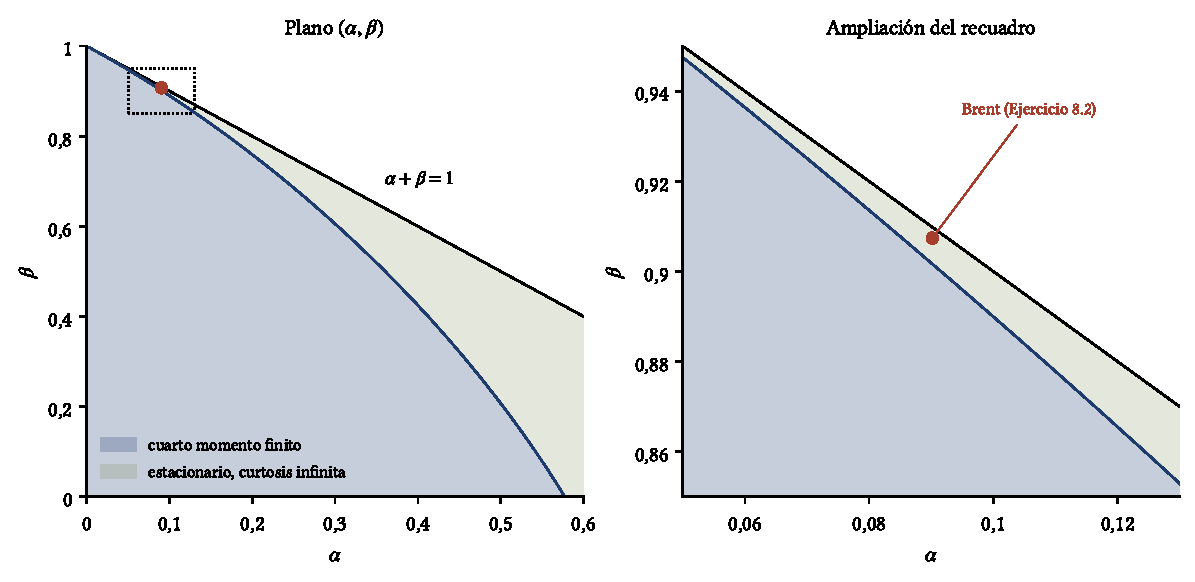
\includegraphics[width=\linewidth]{graficos/cap08_fig_region.pdf}
\caption{Regiones del GARCH(1,1) con innovaciones normales. Azul: estacionario con cuarto momento finito.
Verde claro: estacionario con curtosis infinita. El punto rojo es la estimación del Ejercicio~\ref{ej:garchn}
para el Brent, que cae en la franja de curtosis infinita.}
\label{fig:region}
\end{figure}

\paragraph{IGARCH y EWMA.} Si $\alpha+\beta=1$, el modelo es un GARCH \emph{integrado} (IGARCH): los choques
a la varianza no se disipan y la varianza incondicional no existe. El caso particular con $\omega=0$,
$\alpha=1-\lambda$ y $\beta=\lambda$,
\[
  \sigma_t^2=\lambda\,\sigma_{t-1}^2+(1-\lambda)\,\varepsilon_{t-1}^2,
\]
es la \emph{media móvil ponderada exponencialmente} (EWMA) que popularizó RiskMetrics (J.\,P.~Morgan, 1996)
con $\lambda=0{,}94$ para datos diarios. No se estima: se fija $\lambda$.

% ---------------------------------------------------------------------
\section{Pronóstico de la varianza}
% ---------------------------------------------------------------------

\begin{proposicion}[Pronóstico del GARCH(1,1)]\label{prop:garchpron}
Sea $\phi=\alpha+\beta<1$ y $\E_T[\cdot]=\E[\cdot\mid\mathcal F_T]$. La varianza de $T+1$ se conoce en $T$, y
para $h\ge1$
\[
  \E_T\bigl[\sigma_{T+h}^2\bigr]=\bar\sigma^2+\phi^{\,h-1}\bigl(\sigma_{T+1}^2-\bar\sigma^2\bigr).
\]
\end{proposicion}

\begin{proof}
Para $h=1$ la fórmula da $\sigma_{T+1}^2$, que es conocida en $T$. Supongamos que vale para $h-1\ge1$. Como
$\E_T[\varepsilon_{T+h-1}^2]=\E_T\bigl[\E_{T+h-2}[\sigma_{T+h-1}^2z_{T+h-1}^2]\bigr]=\E_T[\sigma_{T+h-1}^2]$,
\begin{align*}
  \E_T\bigl[\sigma_{T+h}^2\bigr]
    &= \omega+\alpha\,\E_T[\varepsilon_{T+h-1}^2]+\beta\,\E_T[\sigma_{T+h-1}^2]\\
    &= \omega+(\alpha+\beta)\,\E_T[\sigma_{T+h-1}^2]\\
    &= \omega+\phi\bigl[\bar\sigma^2+\phi^{\,h-2}(\sigma_{T+1}^2-\bar\sigma^2)\bigr]\\
    &= \omega+\phi\bar\sigma^2+\phi^{\,h-1}(\sigma_{T+1}^2-\bar\sigma^2).
\end{align*}
Por la Proposición~\ref{prop:garchmom}, $\omega=\bar\sigma^2(1-\phi)$, así que
\begin{align*}
  \omega+\phi\bar\sigma^2 &= \bar\sigma^2-\phi\bar\sigma^2+\phi\bar\sigma^2\\
                          &= \bar\sigma^2,
\end{align*}
y la fórmula vale para $h$. Por inducción, vale para todo $h\ge1$.
\end{proof}

El pronóstico converge geométricamente a $\bar\sigma^2$, desde arriba si hoy la volatilidad está alta y desde
abajo si está baja (Figura~\ref{fig:pronteo}). La rapidez depende solo de la persistencia. La \emph{vida media}
de un choque, el horizonte en que la mitad de la desviación respecto de $\bar\sigma^2$ ha desaparecido, resulta
de
\begin{align*}
  \phi^{\,h} &= \tfrac12,\\
  h\ln\phi   &= \ln\tfrac12,\\
  h          &= \frac{\ln 0{,}5}{\ln\phi}.
\end{align*}
Con $\phi=0{,}97$ la vida media es de 22,8 días; con $\phi=0{,}995$, de 138,3 días.

\begin{figure}[ht]
\centering
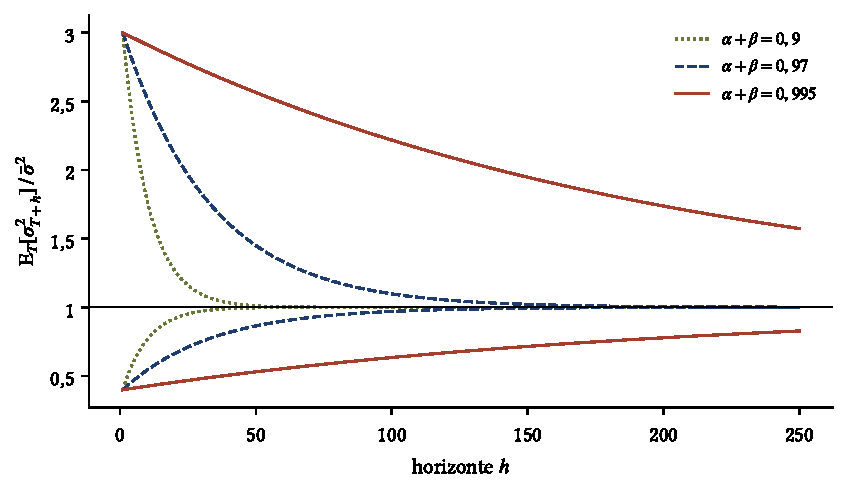
\includegraphics[width=0.74\linewidth]{graficos/cap08_fig_pronostico_teo.pdf}
\caption{Pronóstico de la varianza relativo a su nivel incondicional, partiendo de una varianza tres veces
mayor (curvas superiores) o un 60\,\% menor (inferiores). Cuanto mayor la persistencia $\alpha+\beta$, más lenta
la convergencia.}
\label{fig:pronteo}
\end{figure}

\begin{corolario}[Varianza de un rendimiento de $H$ períodos]\label{cor:varH}
Como los rendimientos no están correlacionados, la varianza condicional del rendimiento acumulado de $T+1$ a
$T+H$ es la suma de las varianzas pronosticadas:
\[
  \sum_{h=1}^{H}\E_T\bigl[\sigma_{T+h}^2\bigr]=H\bar\sigma^2+\bigl(\sigma_{T+1}^2-\bar\sigma^2\bigr)\frac{1-\phi^H}{1-\phi}.
\]
\end{corolario}

\begin{proof}
Sumamos la fórmula de la Proposición~\ref{prop:garchpron}:
\begin{align*}
  \sum_{h=1}^{H}\E_T\bigl[\sigma_{T+h}^2\bigr]
     &= \sum_{h=1}^{H}\bar\sigma^2+\bigl(\sigma_{T+1}^2-\bar\sigma^2\bigr)\sum_{h=1}^{H}\phi^{\,h-1}\\
     &= H\bar\sigma^2+\bigl(\sigma_{T+1}^2-\bar\sigma^2\bigr)\bigl(1+\phi+\dots+\phi^{H-1}\bigr)\\
     &= H\bar\sigma^2+\bigl(\sigma_{T+1}^2-\bar\sigma^2\bigr)\frac{1-\phi^H}{1-\phi}. && \qedhere
\end{align*}
\end{proof}

La regla de la raíz del tiempo del Capítulo~\ref{cap:rendimientos}, $\sqrt{H}\,\sigma_{T+1}$, supone que la
varianza de hoy se mantiene. Si la volatilidad está alta, la regla sobreestima el riesgo de horizonte largo;
si está baja, lo subestima.

% ---------------------------------------------------------------------
\section{Estimación por máxima verosimilitud}
% ---------------------------------------------------------------------

\subsection{La verosimilitud}
La densidad conjunta de la muestra se factoriza en densidades condicionales sucesivas:
\begin{align*}
  f(r_1,\dots,r_T) &= f(r_1)\,f(r_2\mid r_1)\cdots f(r_T\mid r_1,\dots,r_{T-1})\\
                   &= \prod_{t=1}^{T}f(r_t\mid\mathcal F_{t-1}).
\end{align*}
Con $z_t$ normal, $r_t\mid\mathcal F_{t-1}\sim N(\mu,\sigma_t^2)$, y el logaritmo de la verosimilitud es
\begin{align*}
  \ell(\theta) &= \sum_{t=1}^{T}\ell_t(\theta),\\
  \ell_t(\theta) &= -\frac12\Bigl[\ln(2\pi)+\ln\sigma_t^2+\frac{(r_t-\mu)^2}{\sigma_t^2}\Bigr],
\end{align*}
con $\theta=(\mu,\omega,\alpha,\beta)$ y $\sigma_t^2$ calculada con la recursión del GARCH. La recursión
necesita un valor inicial; usamos el de la biblioteca \texttt{arch}, un promedio con pesos $0{,}94^{\,j}$ de los
primeros 75 cuadrados de los residuos (\emph{backcast}). No hay fórmula cerrada para el máximo: se maximiza
numéricamente con las restricciones $\omega>0$, $\alpha,\beta\ge0$.

\subsection{Innovaciones $t$ de Student}
Aun después de dividir entre $\sigma_t$, los residuos de los rendimientos financieros suelen tener colas más
gruesas que la normal. Una alternativa es suponer que $z_t$ sigue una $t$ de Student con $\nu>2$ grados de
libertad, reescalada para que su varianza sea 1.

\begin{proposicion}[$t$ de Student estandarizada]\label{prop:tstd}
Si $X\sim t_\nu$ con $\nu>2$, $\Var(X)=\nu/(\nu-2)$. Por tanto $z=X\sqrt{(\nu-2)/\nu}$ tiene varianza 1 y
densidad
\[
  f(z)=\frac{\Gamma\bigl(\frac{\nu+1}2\bigr)}{\Gamma\bigl(\frac\nu2\bigr)\sqrt{\pi(\nu-2)}}
       \Bigl(1+\frac{z^2}{\nu-2}\Bigr)^{-\frac{\nu+1}2}.
\]
Si $\nu>4$, su curtosis es $3+6/(\nu-4)$.
\end{proposicion}

\begin{proof}
La varianza de la $t_\nu$ y su curtosis $3+6/(\nu-4)$ son resultados estándar. Para el reescalamiento,
\begin{align*}
  \Var(z) &= \frac{\nu-2}{\nu}\,\Var(X)\\
          &= \frac{\nu-2}{\nu}\cdot\frac{\nu}{\nu-2}\\
          &= 1 .
\end{align*}
La curtosis no cambia al multiplicar por una constante. Para la densidad, con $c=\sqrt{(\nu-2)/\nu}$ y $x=z/c$,
el cambio de variable da $f_z(z)=f_X(z/c)/c$. Como
\begin{align*}
  \frac{x^2}{\nu} &= \frac{z^2}{c^2\nu}\\
                  &= \frac{z^2}{\nu-2},\\[4pt]
  c\sqrt{\nu\pi}  &= \sqrt{\frac{\nu-2}{\nu}}\sqrt{\nu\pi}\\
                  &= \sqrt{\pi(\nu-2)},
\end{align*}
al sustituir en la densidad de la $t_\nu$ se obtiene la fórmula del enunciado.
\end{proof}

La contribución de cada observación a la log-verosimilitud, con $z_t=(r_t-\mu)/\sigma_t$, es
\begin{align*}
  \ell_t &= \ln\Gamma\Bigl(\frac{\nu+1}{2}\Bigr)-\ln\Gamma\Bigl(\frac\nu2\Bigr)-\frac12\ln\bigl[\pi(\nu-2)\bigr]
            -\frac12\ln\sigma_t^2-\frac{\nu+1}{2}\ln\Bigl(1+\frac{z_t^2}{\nu-2}\Bigr),
\end{align*}
donde el término $-\frac12\ln\sigma_t^2$ es el jacobiano de pasar de $z_t$ a $r_t$. La
Figura~\ref{fig:tstudentstd} compara la $t$ estandarizada con la normal: en escala lineal casi solo se nota que la
$t$ tiene más pico; en escala logarítmica se ve que sus colas son mucho más altas. Por ejemplo,
$\Pr(|z|>4)$ es $6{,}33\times10^{-5}$ con la normal, pero $1{,}71\times10^{-3}$ con $\nu=8$ y
$4{,}81\times10^{-3}$ con $\nu=4$: entre 27 y 76 veces mayor.

\begin{figure}[ht]
\centering
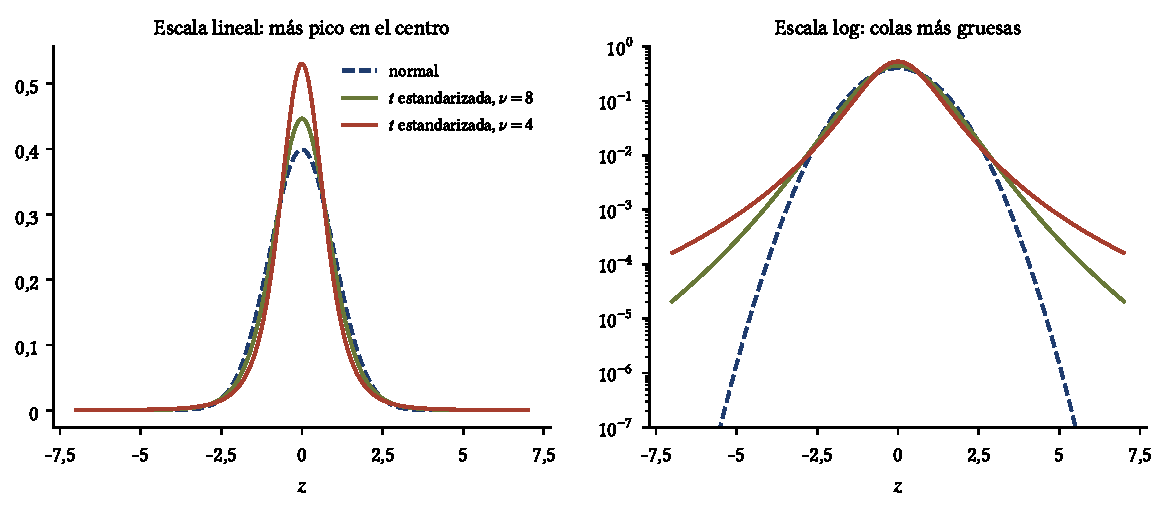
\includegraphics[width=\linewidth]{graficos/cap08_fig_t_student.pdf}
\caption{Densidad de la $t$ de Student estandarizada (varianza 1) con $\nu=4$ y $\nu=8$ frente a la normal
estándar, en escala lineal (izquierda) y logarítmica (derecha).}
\label{fig:tstudentstd}
\end{figure}

\subsection{Cuasi máxima verosimilitud y errores estándar robustos}

¿Qué pasa si se maximiza la verosimilitud normal pero $z_t$ no es normal? Bollerslev y Wooldridge (1992)
mostraron que, si las ecuaciones de la media y la varianza están bien especificadas, el estimador sigue siendo
consistente y asintóticamente normal: es un estimador de \emph{cuasi máxima verosimilitud} (QMLE). Lo que
cambia es su varianza, que toma la forma de ``sándwich'':
\begin{align*}
  \widehat{\Var}(\hat\theta) &= \hat H^{-1}\hat S\,\hat H^{-1},\\
  \hat H &= -\sum_{t=1}^{T}\frac{\partial^2\ell_t(\hat\theta)}{\partial\theta\,\partial\theta'},\\
  \hat S &= \sum_{t=1}^{T}\frac{\partial\ell_t(\hat\theta)}{\partial\theta}\,
            \frac{\partial\ell_t(\hat\theta)}{\partial\theta'} .
\end{align*}
Si el modelo está bien especificado, la igualdad de la información asegura $H=S$ en el límite, y el sándwich
se reduce a $\hat H^{-1}$, la varianza clásica. Con datos financieros conviene reportar siempre la versión
robusta. Calculamos las derivadas numéricamente, con diferencias centrales.

% ---------------------------------------------------------------------
\section{Pruebas de efectos ARCH}
% ---------------------------------------------------------------------

Por la Proposición~\ref{prop:arch1}(iii), bajo un ARCH($q$) los cuadrados $\varepsilon_t^2$ siguen un AR($q$).
Engle (1982) propuso estimar por MCO
\[
  \hat\varepsilon_t^2=a_0+a_1\hat\varepsilon_{t-1}^2+\dots+a_q\hat\varepsilon_{t-q}^2+u_t
\]
y contrastar $H_0:a_1=\dots=a_q=0$ (no hay efectos ARCH) con el estadístico de multiplicadores de Lagrange
\[
  LM=(T-q)\,R^2\ \xrightarrow{d}\ \chi^2_q ,
\]
donde $R^2$ es el de la regresión auxiliar y $T-q$ el número de observaciones que usa. Una alternativa es la
prueba de Ljung-Box aplicada a los cuadrados (McLeod y Li, 1983). Las dos pruebas se aplican también a los
residuos estandarizados $\hat z_t=\hat\varepsilon_t/\hat\sigma_t$ de un modelo estimado: si el modelo capturó la
dinámica de la varianza, $\hat z_t^2$ no debería estar autocorrelacionado.

% ---------------------------------------------------------------------
\section{Evaluación de pronósticos de varianza}
% ---------------------------------------------------------------------

La varianza no se observa, así que los pronósticos $h_t$ se comparan con una aproximación ruidosa, el cuadrado
del rendimiento: $\E_{t-1}[\varepsilon_t^2]=\sigma_t^2$, pero $\varepsilon_t^2=\sigma_t^2z_t^2$ varía mucho
alrededor de $\sigma_t^2$. Patton (2011) muestra que solo algunas funciones de pérdida ordenan bien los
pronósticos con una aproximación ruidosa; dos de ellas son el error cuadrático medio (ECM) y la pérdida QLIKE:
\begin{align*}
  L^{\text{ECM}}(\varepsilon_t^2,h_t)   &= (\varepsilon_t^2-h_t)^2,\\
  L^{\text{QLIKE}}(\varepsilon_t^2,h_t) &= \ln h_t+\frac{\varepsilon_t^2}{h_t}.
\end{align*}

\begin{proposicion}[QLIKE premia el pronóstico correcto]\label{prop:qlike}
Para un pronóstico $h>0$ fijo en $t-1$, $\E_{t-1}\bigl[L^{\text{QLIKE}}(\varepsilon_t^2,h)\bigr]$ se minimiza en
$h=\sigma_t^2$.
\end{proposicion}

\begin{proof}
Como $h$ es conocido en $t-1$:
\begin{align*}
  g(h) &= \E_{t-1}\Bigl[\ln h+\frac{\varepsilon_t^2}{h}\Bigr]\\
       &= \ln h+\frac{\sigma_t^2}{h}.
\end{align*}
Derivamos e igualamos a cero:
\begin{align*}
  g'(h) &= \frac1h-\frac{\sigma_t^2}{h^2}=0,\\
  h     &= \sigma_t^2 .
\end{align*}
Es un mínimo porque la segunda derivada en ese punto es positiva:
\begin{align*}
  g''(h) &= -\frac1{h^2}+\frac{2\sigma_t^2}{h^3},\\
  g''(\sigma_t^2) &= -\frac1{\sigma_t^4}+\frac{2}{\sigma_t^4}\\
                  &= \frac1{\sigma_t^4}>0 . && \qedhere
\end{align*}
\end{proof}

El ECM penaliza los errores en términos absolutos, de modo que unos pocos días de turbulencia dominan el
promedio; QLIKE penaliza los errores relativos y es más estable. Además se usa la \emph{regresión de
Mincer-Zarnowitz}, $\varepsilon_t^2=a+b\,h_t+u_t$: un pronóstico insesgado tiene $a=0$ y $b=1$. Su $R^2$ es
siempre bajo porque $z_t^2$ es muy ruidoso, aunque el pronóstico sea perfecto (Andersen y Bollerslev, 1998).
Para comparar dos modelos se aplica la prueba de Diebold-Mariano del Capítulo~\ref{cap:arma} a la diferencia de
pérdidas.

% ---------------------------------------------------------------------
\section{Ejercicios resueltos}
% ---------------------------------------------------------------------

\begin{ejresuelto}{¿Hay efectos ARCH en el Brent y en el S\&P 500?}\label{ej:archlm}
\enunciado Para los rendimientos diarios del Brent (1987--2026) y mensuales del S\&P 500 (1871--2026), calcule
las primeras autocorrelaciones de $r_t$ y de $r_t^2$ (usando desviaciones respecto de la media), la prueba de
Ljung-Box con 10 rezagos para ambos y la prueba LM de Engle con 5 rezagos.

\solucion
\paso{Paso 1. Autocorrelaciones.} En el Brent, las autocorrelaciones de $r_t$ están entre $-0{,}026$ y
$0{,}015$, mientras que la de $r_t^2$ en el rezago 1 es $0{,}334$ y las siguientes, entre $0{,}053$ y $0{,}075$,
son todas mayores que la banda $\pm0{,}021$. En el S\&P 500 mensual, $r_t^2$ tiene autocorrelaciones de
$0{,}129$, $0{,}155$, $0{,}086$, $0{,}279$ y $0{,}049$ (banda $\pm0{,}045$).

\paso{Paso 2. Pruebas.}
\begin{center}\small
\begin{tabular}{@{}lrrrr@{}}
\toprule
Serie & $Q(10)$ de $r_t$ & $Q(10)$ de $r_t^2$ & $R^2$ auxiliar & LM(5) \\
\midrule
Brent diario      & 25,74 & 1\,718,56 & 0,1199 & 1\,092,93 \\
S\&P 500 mensual  & 168,92 & 450,24 & 0,1002 & 186,61 \\
\bottomrule
\end{tabular}
\end{center}
Para el Brent, el estadístico LM es
\begin{align*}
  LM &= (T-q)\,R^2\\
     &= (9\,121-5)\times0{,}1199\\
     &= 9\,116\times0{,}1199\\
     &\approx 1\,093,
\end{align*}
frente a un valor crítico $\chi^2_5$ al 5\,\% de $11{,}07$. El valor $p$ es del orden de $10^{-234}$.

\paso{Paso 3. Interpretación.} Las dos series rechazan con enorme holgura la ausencia de efectos ARCH. El
$Q(10)$ de $r_t$ del Brent ($p=0{,}004$) también rechaza, pero eso es un espejismo: la prueba clásica supone
homocedasticidad, y la versión robusta del Ejercicio~\ref{ej:acfrob} dio $Q^*(10)=4{,}67$ ($p=0{,}91$). En el
S\&P 500 mensual, la autocorrelación de $0{,}274$ en $r_t$ es el efecto de Working: los precios de la base de
Shiller son promedios mensuales (Capítulo~\ref{cap:arma}).

\codigoweb{cap08_ej01}
\salidaR{cap08_ej01_R.txt}
\lectura{cap08_ej01}

\RvsPy La prueba LM se programa como una regresión auxiliar en los dos lenguajes; Python la comprueba con
\texttt{het\_arch} de \texttt{statsmodels}, que coincide. En R, \texttt{Box.test} devuelve un valor $p$ de cero
cuando es menor que la precisión de la máquina; por eso lo calculamos con \texttt{pchisq(..., lower.tail =
FALSE)}, que trabaja con la cola superior y no pierde precisión.

\begin{figure}[ht]
\centering
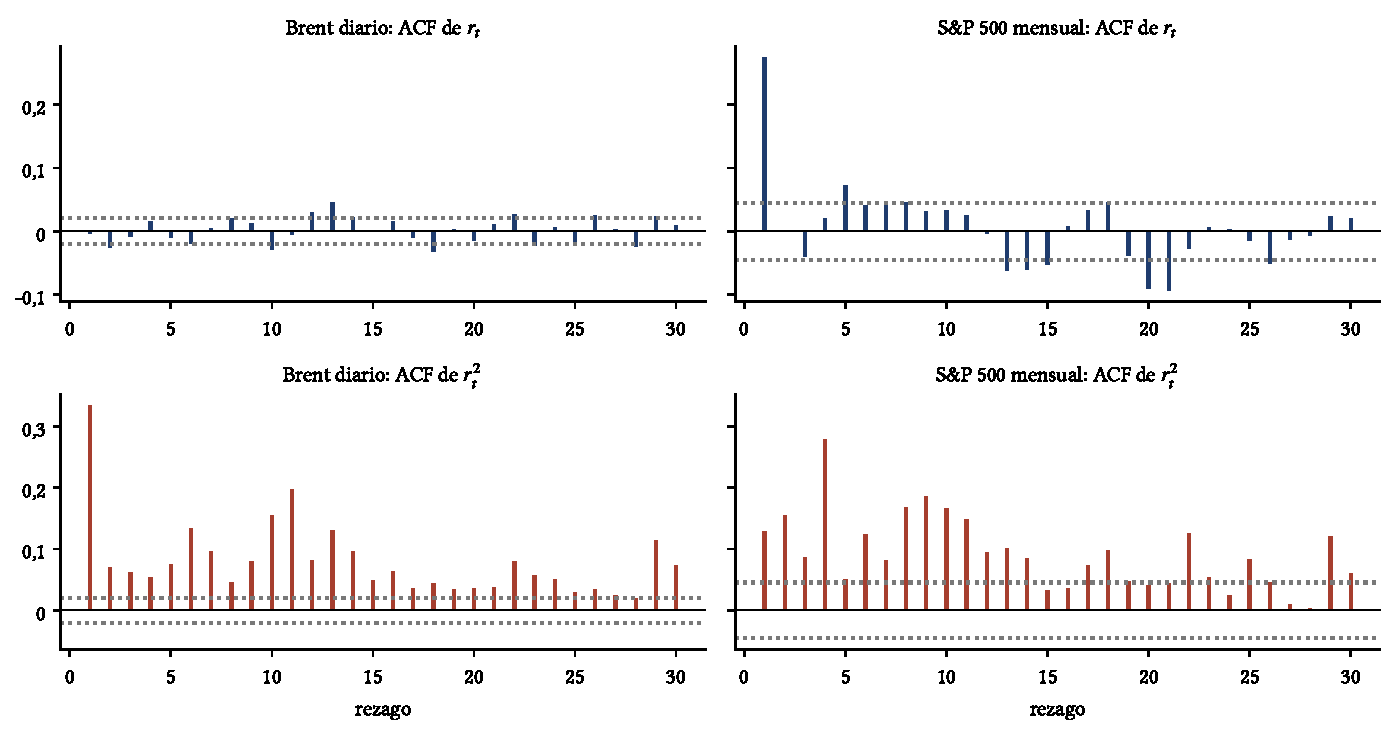
\includegraphics[width=\linewidth]{graficos/cap08_ej01_acf.pdf}
\caption{ACF de los rendimientos (arriba) y de sus cuadrados (abajo) para el Brent diario y el S\&P 500 mensual,
con la banda $\pm1{,}96/\sqrt T$. Los rendimientos del Brent casi no tienen autocorrelación; sus cuadrados sí,
y de forma persistente.}
\label{fig:archacf}
\end{figure}

\begin{conclusion}
Los dos mercados, a frecuencias muy distintas, muestran el patrón que motiva este capítulo: rendimientos casi
impredecibles en nivel y fuertemente predecibles en magnitud.
\end{conclusion}
\end{ejresuelto}

\begin{ejresuelto}{GARCH(1,1) para el Brent, programado a mano}\label{ej:garchn}
\enunciado Estime por máxima verosimilitud un GARCH(1,1) con media constante e innovaciones normales para los
rendimientos diarios del Brent en porcentaje. Programe la verosimilitud y calcule los errores estándar clásicos
(hessiana) y robustos (sándwich). Calcule la persistencia, la vida media, la varianza incondicional implícita y
la condición de cuarto momento. Compare con \texttt{arch}.

\solucion
\paso{Paso 1. Estimación.} El máximo de la log-verosimilitud es $\hat\ell=-20\,074{,}21$, con
\begin{center}\small
\begin{tabular}{@{}lrrrrr@{}}
\toprule
 & Coeficiente & ee hessiana & $t$ & ee robusto & $t$ robusto \\
\midrule
$\mu$      & 0,0346 & 0,0195 & 1,77 & 0,0202 & 1,72 \\
$\omega$   & 0,0517 & 0,0085 & 6,05 & 0,0128 & 4,04 \\
$\alpha$   & 0,0902 & 0,0055 & 16,48 & 0,0094 & 9,64 \\
$\beta$    & 0,9074 & 0,0053 & 172,29 & 0,0087 & 104,79 \\
\bottomrule
\end{tabular}
\end{center}
Los errores robustos son entre 1,5 y 1,7 veces los clásicos en $\omega$, $\alpha$ y $\beta$: las innovaciones no
son normales (lo confirmará el Ejercicio~\ref{ej:garcht}), y la varianza clásica subestima la incertidumbre.

\paso{Paso 2. Persistencia y vida media.}
\begin{align*}
  \hat\phi &= \hat\alpha+\hat\beta\\
           &= 0{,}0902+0{,}9074\\
           &= 0{,}99766,\\[4pt]
  h_{1/2}  &= \frac{\ln0{,}5}{\ln0{,}99766}\\
           &= \frac{-0{,}6931}{-0{,}00234}\\
           &\approx 296 \text{ días}.
\end{align*}
Un choque de volatilidad tarda más de un año bursátil en reducirse a la mitad.

\paso{Paso 3. Varianza incondicional.}
\begin{align*}
  \hat{\bar\sigma}^2 &= \frac{\hat\omega}{1-\hat\alpha-\hat\beta}\\
                     &= \frac{0{,}0517}{0{,}00234}\\
                     &= 22{,}11,
\end{align*}
es decir, una volatilidad anual de $\sqrt{252\times22{,}11}=74{,}6$\,\%, muy por encima de la varianza muestral
($7{,}31$; volatilidad anual de 42,9\,\%). La discrepancia es una advertencia: cuando $\alpha+\beta$ está tan
cerca de uno, $\bar\sigma^2$ es el cociente de dos números pequeños y se estima con muy poca precisión; además,
el modelo atribuye a la varianza de largo plazo los episodios extremos de 2020 y de 2026.

\paso{Paso 4. Cuarto momento.}
\begin{align*}
  (\hat\alpha+\hat\beta)^2+2\hat\alpha^2 &= 0{,}99766^2+2(0{,}0902)^2\\
                                         &= 0{,}99533+0{,}01628\\
                                         &= 1{,}0116>1 .
\end{align*}
El modelo estimado implica curtosis infinita: es el punto rojo de la Figura~\ref{fig:region}.

\paso{Paso 5. La trayectoria de la volatilidad.} Omitiendo el primer año, que depende del valor inicial, la
volatilidad anualizada $\sqrt{252\,\hat\sigma_t^2}$ va de un mínimo de 14,8\,\% (5 de junio de 2014) a un máximo
de 395\,\% (23 de abril de 2020). Dos días antes, en pleno colapso de la demanda por la pandemia, el Brent
había pasado de 17,36 a 9,12 dólares en una sola sesión, un rendimiento logarítmico de $-64$\,\%, y al día
siguiente subió a 13,77 (Figura~\ref{fig:garchvol}).

\codigoweb{cap08_ej02}
\salidaR{cap08_ej02_R.txt}
\lectura{cap08_ej02}

\RvsPy Las dos implementaciones recorren la misma recursión con un bucle explícito y usan el mismo valor
inicial que \texttt{arch}, por lo que los tres resultados coinciden en todas las cifras mostradas. Los
optimizadores sí difieren: en R usamos \texttt{nlminb}, que llegó al mismo máximo que \texttt{arch} con más
precisión que \texttt{optim(method = "L-BFGS-B")}; en Python, \texttt{minimize} de \texttt{scipy} con
\texttt{L-BFGS-B}. Con ambos conviene fijar tolerancias estrictas, porque la verosimilitud es muy plana en la
dirección de $\omega/(1-\alpha-\beta)$. La hessiana y los scores se calculan con las mismas diferencias
centrales en los dos lenguajes.

\begin{figure}[ht]
\centering
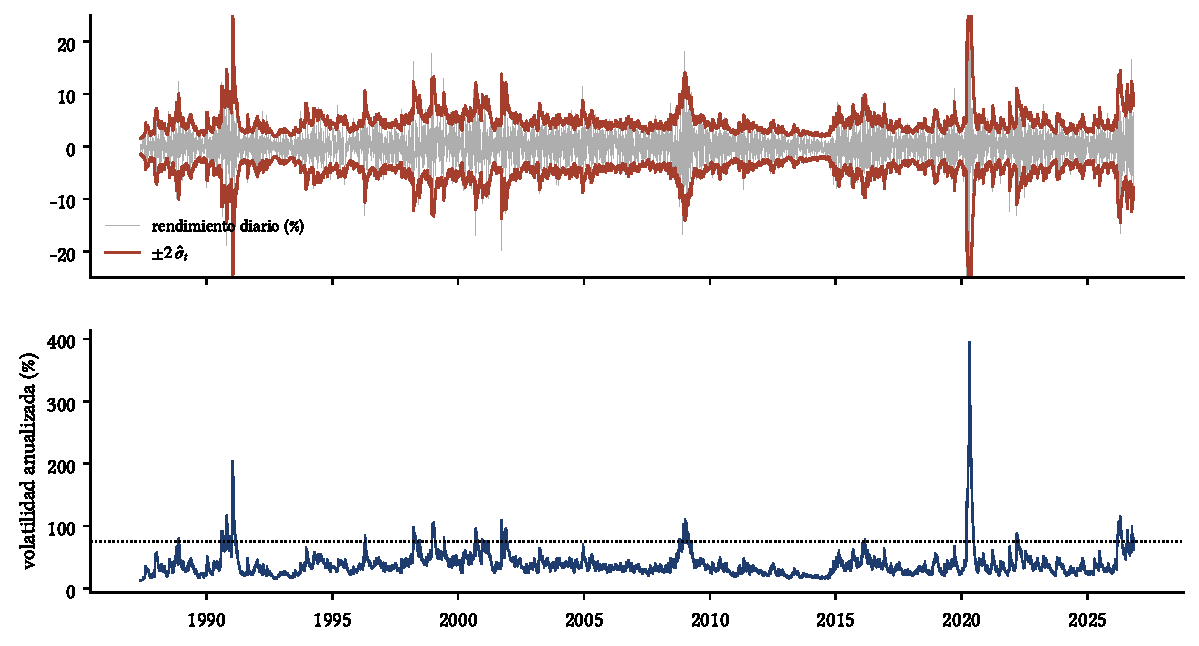
\includegraphics[width=\linewidth]{graficos/cap08_ej02_volatilidad.pdf}
\caption{Arriba: rendimientos diarios del Brent con las bandas $\pm2\hat\sigma_t$ del GARCH(1,1) (eje recortado a
$\pm25$\,\%). Abajo: volatilidad anualizada estimada; la línea punteada es la implícita en $\hat{\bar\sigma}^2$.}
\label{fig:garchvol}
\end{figure}

\begin{conclusion}
El GARCH(1,1) reproduce el agrupamiento de volatilidad del Brent con tres parámetros. La volatilidad es muy
persistente ($\alpha+\beta=0{,}998$) y varía enormemente en el tiempo: decir que ``la volatilidad del petróleo
es de 43\,\% anual'' oculta que ha oscilado entre 15\,\% y casi 400\,\%.
\end{conclusion}
\end{ejresuelto}

\begin{ejresuelto}{Innovaciones $t$ de Student y diagnóstico}\label{ej:garcht}
\enunciado Reestime el modelo con innovaciones $t$ de Student estandarizadas. Compare con el modelo normal
mediante AIC y BIC. Calcule los residuos estandarizados $\hat z_t=(r_t-\hat\mu)/\hat\sigma_t$ y compare su
asimetría, curtosis, prueba de Jarque-Bera y pruebas de Ljung-Box con las de los rendimientos originales.

\solucion
\paso{Paso 1. Estimación.} Con errores robustos:
\begin{center}\small
\begin{tabular}{@{}lrrr@{}}
\toprule
 & Coeficiente & ee robusto & $t$ \\
\midrule
$\mu$    & 0,0522 & 0,0184 & 2,83 \\
$\omega$ & 0,0593 & 0,0118 & 5,03 \\
$\alpha$ & 0,0832 & 0,0074 & 11,24 \\
$\beta$  & 0,9123 & 0,0072 & 127,41 \\
$\nu$    & 5,2295 & 0,2784 & 18,78 \\
\bottomrule
\end{tabular}
\end{center}
La persistencia baja a $0{,}99554$ (vida media de 155 días). Con $\hat\nu=5{,}23$, la curtosis de la $t$
estandarizada es
\begin{align*}
  3+\frac{6}{\hat\nu-4} &= 3+\frac{6}{1{,}2295}\\
                        &= 7{,}88 .
\end{align*}

\paso{Paso 2. Comparación.}
\begin{center}\small
\begin{tabular}{@{}lrrr@{}}
\toprule
Modelo & $\hat\ell$ & AIC & BIC \\
\midrule
GARCH normal & $-20\,074{,}21$ & 40\,156,43 & 40\,184,90 \\
GARCH-$t$    & $-19\,752{,}61$ & 39\,515,21 & 39\,550,81 \\
\bottomrule
\end{tabular}
\end{center}
El parámetro adicional aumenta la log-verosimilitud en $321{,}6$ puntos, y los dos criterios prefieren la $t$
por más de 600 puntos. (Una prueba de razón de verosimilitudes no es estándar aquí, porque la normal
corresponde a $\nu=\infty$, en la frontera del espacio de parámetros; pero con una diferencia de esta
magnitud no hace falta.)

\paso{Paso 3. Diagnóstico.}
\begin{center}\small
\begin{tabular}{@{}lrrrrr@{}}
\toprule
Serie & Asimetría & Curtosis & Jarque-Bera & $Q(10)$ nivel & $Q(10)$ cuadrados \\
\midrule
$r_t$        & $-1{,}49$ & 55,97 & 1\,069\,541 & 25,74 & 1\,718,56 \\
$\hat z_t$   & $-0{,}20$ & 5,48 & 2\,388 & 22,64 & 14,93 \\
\bottomrule
\end{tabular}
\end{center}
El modelo absorbe casi toda la dependencia de los cuadrados: $Q(10)$ baja de $1\,718{,}56$ a $14{,}93$
($p=0{,}135$). La curtosis cae de 56 a 5,5: la mayor parte de las colas gruesas de los rendimientos se explica
por la volatilidad cambiante. Lo que queda (una curtosis de 5,5, aún mayor que 3) es lo que la $t$ de Student
modela. Persiste una autocorrelación débil en el nivel ($p=0{,}012$), que se concentra en el rezago 2 y
podría modelarse con un término AR en la media, aunque su tamaño ($-0{,}026$) es económicamente irrelevante.

\paso{Paso 4. Las colas.} Hay $0{,}00362\times9\,121=33$ días con $|\hat z_t|>4$. La normal predice
$6{,}33\times10^{-5}\times9\,121=0{,}58$ días; la $t$ con $\nu=5{,}23$, $0{,}00335\times9\,121=31$ días. El
gráfico cuantil-cuantil de la Figura~\ref{fig:garchqq} lo muestra: frente a la normal los puntos se curvan en
los extremos; frente a la $t$ siguen la diagonal.

\codigoweb{cap08_ej03}
\salidaR{cap08_ej03_R.txt}
\lectura{cap08_ej03}

\RvsPy La función \texttt{lgamma} de R equivale a \texttt{gammaln} de \texttt{scipy.special}; se usan los
logaritmos de la función gamma para evitar desbordamientos. En Python, \texttt{stats.t.ppf(u, nu)} da los
cuantiles de la $t$ sin estandarizar, que multiplicamos por $\sqrt{(\nu-2)/\nu}$ para el gráfico.

\begin{figure}[ht]
\centering
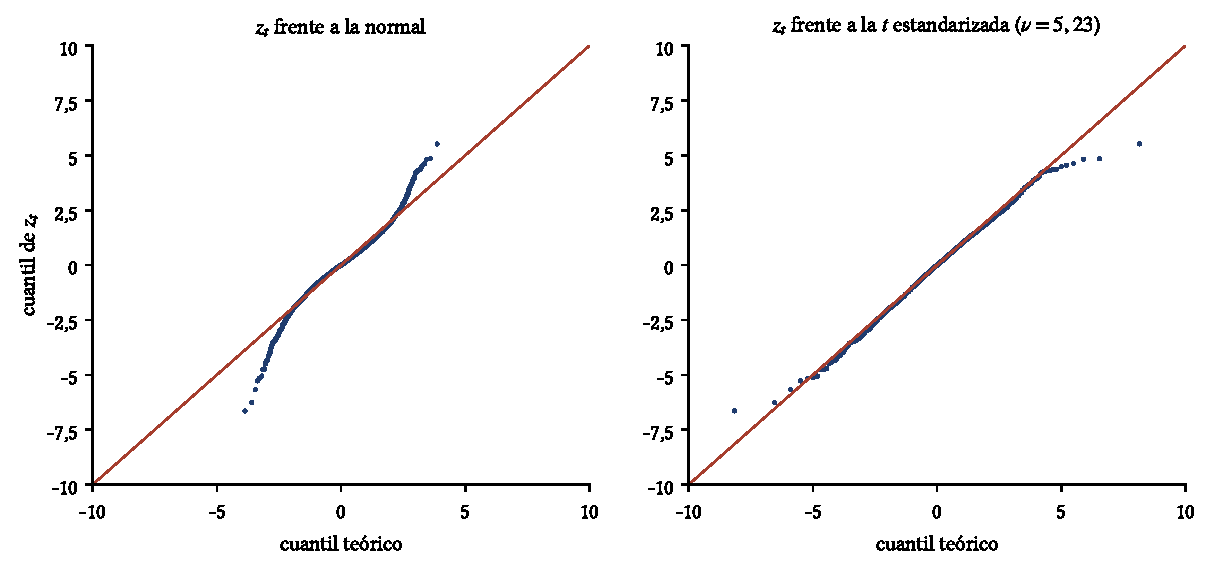
\includegraphics[width=\linewidth]{graficos/cap08_ej03_qq.pdf}
\caption{Gráficos cuantil-cuantil de los residuos estandarizados del GARCH-$t$ frente a la normal (izquierda) y
frente a la $t$ estandarizada con $\hat\nu=5{,}23$ (derecha).}
\label{fig:garchqq}
\end{figure}

\begin{conclusion}
Las innovaciones normales no bastan para el Brent: aun condicionando en la volatilidad, los choques extremos son
más frecuentes de lo que permite la normal. La $t$ de Student, con un solo parámetro adicional, reproduce bien
las colas y mejora drásticamente la verosimilitud.
\end{conclusion}
\end{ejresuelto}

\begin{ejresuelto}{Pronóstico de la volatilidad del Brent}\label{ej:garchpron}
\enunciado Con el GARCH-$t$ estimado con toda la muestra, pronostique la varianza del Brent para los próximos
252 días hábiles a partir del 3 de noviembre de 2026. Calcule la volatilidad de un mes (21 días) y de un año
(252 días), y compárelas con la regla de la raíz del tiempo.

\solucion
\paso{Paso 1. La varianza de mañana.} El último rendimiento es $r_T=-0{,}336$\,\%, de modo que
$\hat\varepsilon_T^2=(r_T-\hat\mu)^2=0{,}1505$, y la varianza estimada para ese día es $\hat\sigma_T^2=24{,}7793$.
Entonces
\begin{align*}
  \hat\sigma_{T+1}^2 &= \hat\omega+\hat\alpha\,\hat\varepsilon_T^2+\hat\beta\,\hat\sigma_T^2\\
                     &= 0{,}0593+0{,}0832\times0{,}1505+0{,}9123\times24{,}7793\\
                     &= 22{,}678,
\end{align*}
una volatilidad diaria de $4{,}76$\,\% y anualizada de $\sqrt{252\times22{,}678}=75{,}6$\,\%. El año 2026 ha
sido excepcional en los datos: el Brent empezó el año en 62 dólares, llegó a 138 en abril y ha tenido
movimientos diarios de más de 10\,\% en ambas direcciones.

\paso{Paso 2. Nivel de largo plazo.}
\begin{align*}
  \hat{\bar\sigma}^2 &= \frac{0{,}0593}{1-0{,}99554}\\
                     &= 13{,}286,
\end{align*}
es decir, 57,9\,\% anual.

\paso{Paso 3. Pronóstico a 21 días.} Por la Proposición~\ref{prop:garchpron}, con $\hat\phi^{20}=0{,}9145$:
\begin{align*}
  \E_T[\sigma_{T+21}^2] &= 13{,}286+0{,}9145\times(22{,}678-13{,}286)\\
                        &= 13{,}286+0{,}9145\times9{,}392\\
                        &= 13{,}286+8{,}589\\
                        &= 21{,}874 .
\end{align*}
La siguiente tabla resume la trayectoria:
\begin{center}\small
\begin{tabular}{@{}rrr@{}}
\toprule
$h$ (días) & $\E_T[\sigma^2_{T+h}]$ & Volatilidad anualizada \\
\midrule
1   & 22,678 & 75,6\,\% \\
21  & 21,874 & 74,2\,\% \\
63  & 20,404 & 71,7\,\% \\
126 & 18,657 & 68,6\,\% \\
252 & 16,344 & 64,2\,\% \\
\bottomrule
\end{tabular}
\end{center}

\paso{Paso 4. Volatilidad acumulada.} Por el Corolario~\ref{cor:varH}, con $(1-\hat\phi^{21})/(1-\hat\phi)=20{,}089$:
\begin{align*}
  \sum_{h=1}^{21}\E_T[\sigma_{T+h}^2] &= 21\times13{,}286+9{,}392\times20{,}089\\
                                      &= 279{,}01+188{,}67\\
                                      &= 467{,}68,\\[4pt]
  \sqrt{467{,}68} &= 21{,}63 .
\end{align*}
La volatilidad del mes es, por tanto, de 21,63\,\%. La regla de la raíz daría $\sqrt{21\times22{,}678}=21{,}82$\,\%, casi lo mismo. A un año, en cambio, el GARCH da
una volatilidad de $\sqrt{4\,771}=69{,}07$\,\% frente a $75{,}60$\,\% de la regla: como la volatilidad actual está
por encima de su nivel normal, la regla de la raíz sobreestima el riesgo de largo plazo.

\codigoweb{cap08_ej04}
\salidaR{cap08_ej04_R.txt}
\lectura{cap08_ej04}

\RvsPy El método \texttt{forecast} de \texttt{arch} implementa la misma fórmula y coincide con nuestro cálculo
(las diferencias en la tercera decimal a 252 días vienen de diferencias mínimas en los parámetros que
encuentran los optimizadores, que la potencia $\hat\phi^{\,h}$ amplifica). En Python, la figura sitúa los
pronósticos en días hábiles futuros con \texttt{pd.bdate\_range}.

\begin{figure}[ht]
\centering
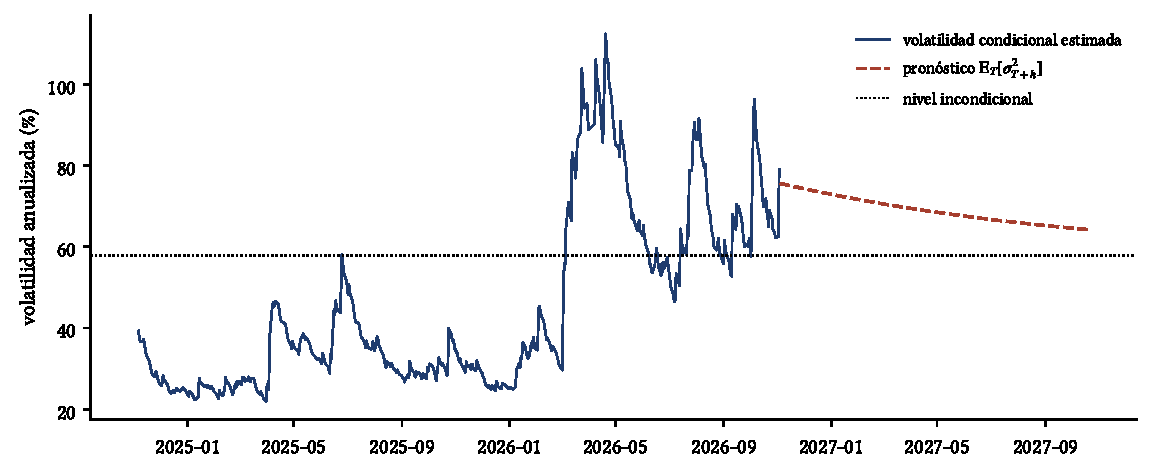
\includegraphics[width=0.92\linewidth]{graficos/cap08_ej04_pronostico.pdf}
\caption{Volatilidad condicional anualizada del Brent en los dos últimos años de la muestra y su pronóstico a
252 días hábiles. El pronóstico desciende lentamente hacia el nivel incondicional (línea punteada).}
\label{fig:garchpron}
\end{figure}

\begin{conclusion}
Con una persistencia de $0{,}9955$, el pronóstico de volatilidad del Brent desciende despacio: un año después
todavía está por encima de su nivel de largo plazo. Para horizontes de días, la regla de la raíz es una buena
aproximación; para horizontes de meses, conviene usar el pronóstico del modelo.
\end{conclusion}
\end{ejresuelto}

\begin{ejresuelto}{¿Pronostica mejor el GARCH? Evaluación fuera de muestra}\label{ej:garchfuera}
\enunciado Estime un GARCH(1,1) normal con los datos del Brent hasta el 31 de diciembre de 2015 y, con esos
parámetros fijos, genere pronósticos a un día para 2016--2026. Compárelos con la EWMA de RiskMetrics
($\lambda=0{,}94$) y con la varianza histórica de los 250 días previos, usando ECM, QLIKE, la regresión de
Mincer-Zarnowitz y la prueba de Diebold-Mariano sobre QLIKE.

\solucion
\paso{Paso 1. Estimación.} Con 6\,370 días, $\hat\omega=0{,}0265$, $\hat\alpha=0{,}0697$ y $\hat\beta=0{,}9300$:
la persistencia dentro de la muestra es $0{,}9997$, casi un IGARCH. La muestra de evaluación tiene 2\,751 días
(4 de enero de 2016 a 3 de noviembre de 2026).

\paso{Paso 2. Pérdidas.}
\begin{center}\small
\begin{tabular}{@{}lrrrrr@{}}
\toprule
Modelo & ECM & QLIKE & $a$ (MZ) & $b$ (MZ) & $R^2$ (MZ) \\
\midrule
GARCH(1,1)          & 7\,947,35 & 2,7237 & 2,530 & 0,736 & 0,0664 \\
EWMA                & 7\,967,32 & 2,7454 & 2,673 & 0,747 & 0,0626 \\
Ventana de 250 días & 8\,476,37 & 3,0766 & 6,552 & 0,386 & 0,0032 \\
\bottomrule
\end{tabular}
\end{center}
El GARCH tiene la menor pérdida con los dos criterios; la EWMA queda muy cerca y la ventana móvil, lejos.

\paso{Paso 3. Diebold-Mariano.} Con $d_t=L_t^{\text{rival}}-L_t^{\text{GARCH}}$ en QLIKE y errores de
Newey-West:
\begin{center}\small
\begin{tabular}{@{}lrr@{}}
\toprule
Comparación & $\bar d$ & $t$ \\
\midrule
GARCH frente a EWMA        & 0,0217 & 3,70 \\
GARCH frente a ventana 250 & 0,3529 & 3,73 \\
\bottomrule
\end{tabular}
\end{center}
Las dos diferencias son significativas: el GARCH pronostica mejor. La ventaja sobre la EWMA es pequeña en nivel
(menos del 1\,\% de la pérdida media), pero sistemática.

\paso{Paso 4. Mincer-Zarnowitz.} Ningún modelo es insesgado: $\hat b<1$ indica que, cuando pronostican varianzas
altas, la realizada promedio es menor (sobrerreaccionan a los choques). La ventana móvil es la peor: su
$\hat b=0{,}386$ y su $R^2$ de $0{,}003$ revelan que apenas sigue a la volatilidad. Los $R^2$ bajos de todos los
modelos son los esperables con un aproximante tan ruidoso como $\varepsilon_t^2$.

\codigoweb{cap08_ej05}
\salidaR{cap08_ej05_R.txt}
\lectura{cap08_ej05}

\RvsPy Los pronósticos fuera de muestra se obtienen haciendo correr la recursión del GARCH sobre toda la
serie con los parámetros fijos: $\hat\sigma_t^2$ solo usa datos hasta $t-1$, así que no hay mirada al futuro. Lo
mismo vale para la EWMA y para la ventana móvil, que en R y en Python se calculan con bucles idénticos.

\begin{figure}[ht]
\centering
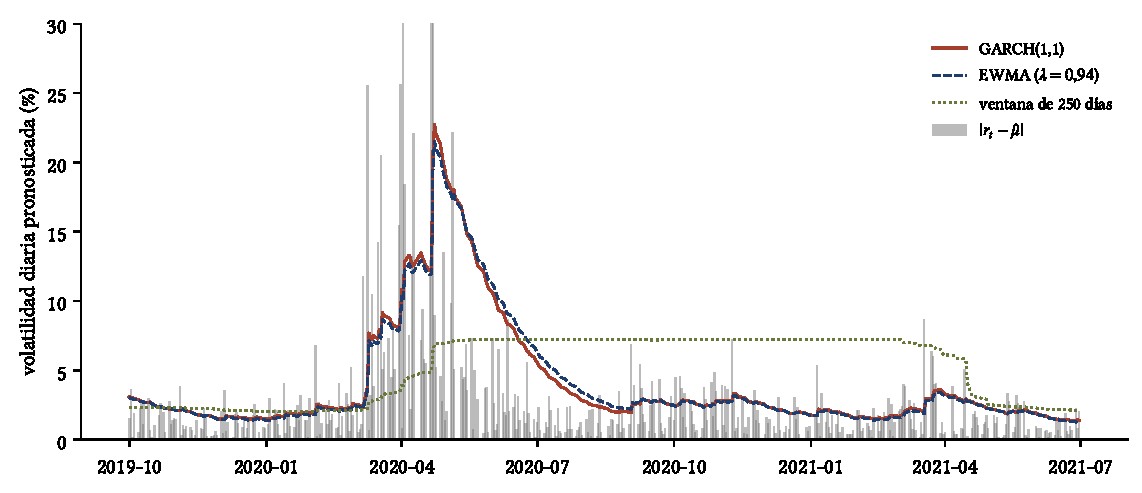
\includegraphics[width=0.92\linewidth]{graficos/cap08_ej05_fuera_muestra.pdf}
\caption{Pronósticos de volatilidad diaria del Brent entre octubre de 2019 y junio de 2021, frente al valor
absoluto del rendimiento (barras). El GARCH y la EWMA reaccionan en pocos días al choque de 2020; la ventana de
250 días reacciona tarde y se mantiene alta durante un año, hasta que el choque sale de la ventana.}
\label{fig:garchfuera}
\end{figure}

\begin{conclusion}
Fuera de muestra, el GARCH(1,1) supera con significancia a la EWMA y a la varianza histórica. La ventana móvil
es la peor por construcción: pondera igual un dato de hace once meses que uno de ayer, y deja de recordar un
choque de golpe. La EWMA, que no requiere estimación, es una alternativa casi tan buena como el GARCH.
\end{conclusion}
\end{ejresuelto}

% ---------------------------------------------------------------------
\section{Ejercicios propuestos}
% ---------------------------------------------------------------------

\begin{enumerate}[label=\textbf{\thechapter.\arabic*},leftmargin=*,itemsep=6pt]
  \item Para un ARCH(1) normal con $\omega=0{,}2$ y $\alpha=0{,}3$, calcule la varianza incondicional y la
  curtosis. \textit{Respuesta: $0{,}2857$ y $3{,}740$.}

  \item Para un GARCH(1,1) normal con $\omega=0{,}02$, $\alpha=0{,}05$ y $\beta=0{,}93$, calcule la varianza
  incondicional, la vida media y la curtosis. \textit{Respuesta: $1$; $34{,}3$ períodos; $3{,}434$.}

  \item Bollerslev (1988) muestra que, en un GARCH(1,1), la primera autocorrelación de $\varepsilon_t^2$ es
  $\rho_1=\alpha(1-\alpha\beta-\beta^2)/(1-2\alpha\beta-\beta^2)$. Calcúlela con los parámetros del ejercicio
  anterior y verifíquela simulando dos millones de observaciones. \textit{Respuesta: $0{,}105$.}

  \item Demuestre que en la EWMA el pronóstico de la varianza es plano:
  $\E_T[\sigma_{T+h}^2]=\sigma_{T+1}^2$ para todo $h\ge1$. ¿Qué implica para la regla de la raíz del tiempo?

  \item Demuestre que la pérdida ECM también se minimiza en $h=\sigma_t^2$. ¿Por qué entonces se prefiere QLIKE
  cuando hay días de turbulencia extrema?

  \item Demuestre que la varianza de un ARCH(2) es $\omega/(1-\alpha_1-\alpha_2)$ y escriba $\varepsilon_t^2$
  como un AR(2).

  \item \emph{(Con datos del BCRP.)} Estime un GARCH(1,1)-$t$ para los rendimientos diarios del tipo de cambio
  interbancario sol/dólar. Compare la persistencia y los grados de libertad con los del Brent. ¿Cómo se refleja
  la intervención cambiaria del BCRP en la volatilidad estimada?

  \item \emph{(Simulación.)} Simule 500 muestras de $T=2\,000$ observaciones de un GARCH(1,1)-$t$ con los
  parámetros del Ejercicio~\ref{ej:garcht} y reestime el modelo en cada una con su función propia. Dibuje la
  distribución de $\hat\alpha+\hat\beta$ y de $\hat\nu$. ¿Están sesgadas?

  \item \emph{(Con datos.)} Repita el Ejercicio~\ref{ej:garchfuera} con el GARCH-$t$ y reestimando los
  parámetros cada año con una ventana creciente. ¿Cambia la clasificación de los modelos?
\end{enumerate}

% ---------------------------------------------------------------------
\section{Resumen de fórmulas}
% ---------------------------------------------------------------------

\begin{table}[H]
\centering\small
\begin{tabular}{@{}ll@{}}
\toprule
Concepto & Fórmula \\
\midrule
ARCH(1) & $\sigma^2=\omega/(1-\alpha)$;\quad $\kappa=3(1-\alpha^2)/(1-3\alpha^2)$ \\
GARCH(1,1) & $\sigma_t^2=\omega+\alpha\varepsilon_{t-1}^2+\beta\sigma_{t-1}^2$;\quad $\bar\sigma^2=\omega/(1-\alpha-\beta)$ \\
Curtosis GARCH(1,1) & $\kappa=3[1-(\alpha+\beta)^2]/[1-(\alpha+\beta)^2-2\alpha^2]$ \\
EWMA & $\sigma_t^2=\lambda\sigma_{t-1}^2+(1-\lambda)\varepsilon_{t-1}^2$,\quad $\lambda=0{,}94$ \\
Pronóstico & $\E_T[\sigma_{T+h}^2]=\bar\sigma^2+(\alpha+\beta)^{h-1}(\sigma_{T+1}^2-\bar\sigma^2)$ \\
Vida media & $h_{1/2}=\ln0{,}5/\ln(\alpha+\beta)$ \\
Log-verosimilitud normal & $\ell_t=-\frac12[\ln2\pi+\ln\sigma_t^2+\varepsilon_t^2/\sigma_t^2]$ \\
Varianza QMLE & $\hat H^{-1}\hat S\hat H^{-1}$ \\
Prueba LM de Engle & $(T-q)R^2\sim\chi^2_q$ \\
Pérdida QLIKE & $\ln h_t+\varepsilon_t^2/h_t$ \\
\bottomrule
\end{tabular}
\caption{Fórmulas principales del Capítulo 8.}
\end{table}

\section*{Referencias}
\begin{itemize}[leftmargin=*]
  \item Andersen, T. G. y Bollerslev, T. (1998). Answering the skeptics: Yes, standard volatility models do
        provide accurate forecasts. \emph{International Economic Review}, 39(4), 885--905.
  \item Bollerslev, T. (1986). Generalized autoregressive conditional heteroskedasticity. \emph{Journal of
        Econometrics}, 31(3), 307--327.
  \item Bollerslev, T. (1988). On the correlation structure for the generalized autoregressive conditional
        heteroskedastic process. \emph{Journal of Time Series Analysis}, 9(2), 121--131.
  \item Bollerslev, T. y Wooldridge, J. M. (1992). Quasi-maximum likelihood estimation and inference in dynamic
        models with time-varying covariances. \emph{Econometric Reviews}, 11(2), 143--172.
  \item Engle, R. F. (1982). Autoregressive conditional heteroscedasticity with estimates of the variance of
        United Kingdom inflation. \emph{Econometrica}, 50(4), 987--1007.
  \item J.\,P.~Morgan/Reuters (1996). \emph{RiskMetrics: Technical Document}, 4.ª ed. Nueva York.
  \item McLeod, A. I. y Li, W. K. (1983). Diagnostic checking ARMA time series models using squared-residual
        autocorrelations. \emph{Journal of Time Series Analysis}, 4(4), 269--273.
  \item Patton, A. J. (2011). Volatility forecast comparison using imperfect volatility proxies.
        \emph{Journal of Econometrics}, 160(1), 246--256.
\end{itemize}

% =====================================================================
%  Capítulo 9. Extensiones del GARCH: asimetría y prima por riesgo
% =====================================================================
\chapter[Extensiones del GARCH]{Extensiones del GARCH: asimetría, efecto apalancamiento y GARCH en media}\label{cap:asimetria}

\section*{Objetivos de aprendizaje}
Al terminar este capítulo, el lector podrá:
\begin{enumerate}[label=\arabic*.,leftmargin=*]
  \item Explicar el efecto apalancamiento y la retroalimentación de la volatilidad, y detectar la asimetría con
        correlaciones cruzadas y con las pruebas de sesgo de signo de Engle y Ng.
  \item Derivar las propiedades de los modelos GJR-GARCH y EGARCH y estimarlos por máxima verosimilitud.
  \item Construir e interpretar curvas de impacto de noticias.
  \item Estimar un GARCH en media y relacionar su coeficiente con la aversión al riesgo del inversionista.
\end{enumerate}

\section*{Motivación}
En el GARCH(1,1) la varianza de mañana depende de $\varepsilon_{t-1}^2$: una caída de 3\,\% y una subida de
3\,\% tienen el mismo efecto. En los mercados de acciones no es así. Las caídas elevan la volatilidad mucho
más que las subidas, y la volatilidad implícita (el VIX) se dispara en las crisis y se calma en los auges. Este
capítulo estudia esa \emph{asimetría} y los modelos que la capturan. También aborda una pregunta central de las
finanzas: si los inversionistas exigen un rendimiento mayor cuando el riesgo es mayor, ¿se ve esa relación en
los datos?

\paragraph{Datos del capítulo.} Rendimientos diarios del S\&P 500 (cierre ajustado de Yahoo Finance, 1999--2018,
$T=5\,030$) y del Brent (1987--2026); el VIX diario de la CBOE, y el exceso de rendimiento mensual del mercado
de EE.\,UU. de la base de Kenneth French (julio de 1926 a noviembre de 2018).

% ---------------------------------------------------------------------
\section{¿Por qué las caídas elevan más la volatilidad?}
% ---------------------------------------------------------------------

Black (1976) propuso la primera explicación, conocida como \emph{efecto apalancamiento}.

\begin{proposicion}[Apalancamiento financiero y volatilidad]\label{prop:black}
Sea una empresa con activos de valor $V$, financiados con deuda $D$ sin riesgo y fija, y acciones de valor
$E=V-D$. Si la volatilidad de los activos es $\sigma_V$, la de las acciones es
\[
  \sigma_E=\frac{V}{E}\,\sigma_V=\Bigl(1+\frac DE\Bigr)\sigma_V .
\]
\end{proposicion}

\begin{proof}
Como $D$ no cambia, todo cambio en el valor de los activos recae en las acciones:
\begin{align*}
  dE &= dV .
\end{align*}
Dividimos entre $E$ y multiplicamos y dividimos por $V$:
\begin{align*}
  \frac{dE}{E} &= \frac{dV}{E}\\
               &= \frac VE\cdot\frac{dV}{V}.
\end{align*}
El rendimiento de las acciones es $V/E$ veces el de los activos, de modo que su desviación estándar es
\begin{align*}
  \sigma_E &= \frac VE\,\sigma_V\\
           &= \frac{E+D}{E}\,\sigma_V\\
           &= \Bigl(1+\frac DE\Bigr)\sigma_V . && \qedhere
\end{align*}
\end{proof}

Cuando el precio de la acción cae, $D/E$ sube y la acción se vuelve más volátil. El panel izquierdo de la
Figura~\ref{fig:apalanc} lo dibuja con $D=50$ y $\sigma_V=20$\,\%: con $E=100$ la volatilidad de la acción es
$1{,}5\times20=30$\,\%; si las acciones caen a 50, sube a $2\times20=40$\,\%; si caen a 20, a
$3{,}5\times20=70$\,\%. La relación es convexa: cada caída adicional eleva la volatilidad más que la anterior.

El apalancamiento, sin embargo, no basta para explicar la magnitud de la asimetría observada, que también
aparece en empresas sin deuda (Figlewski y Wang, 2000). Una segunda explicación invierte la causalidad: la
\emph{retroalimentación de la volatilidad} (Campbell y Hentschel, 1992). Si llega una noticia que eleva la
volatilidad esperada y los inversionistas exigen más rendimiento por más riesgo, el precio debe caer hoy para
que el rendimiento esperado suba. En un caso la caída del precio causa la volatilidad; en el otro, la
volatilidad causa la caída. Las dos predicen el mismo signo, y en la práctica se habla de ``efecto
apalancamiento'' para cualquier asimetría de este tipo.

\begin{figure}[ht]
\centering
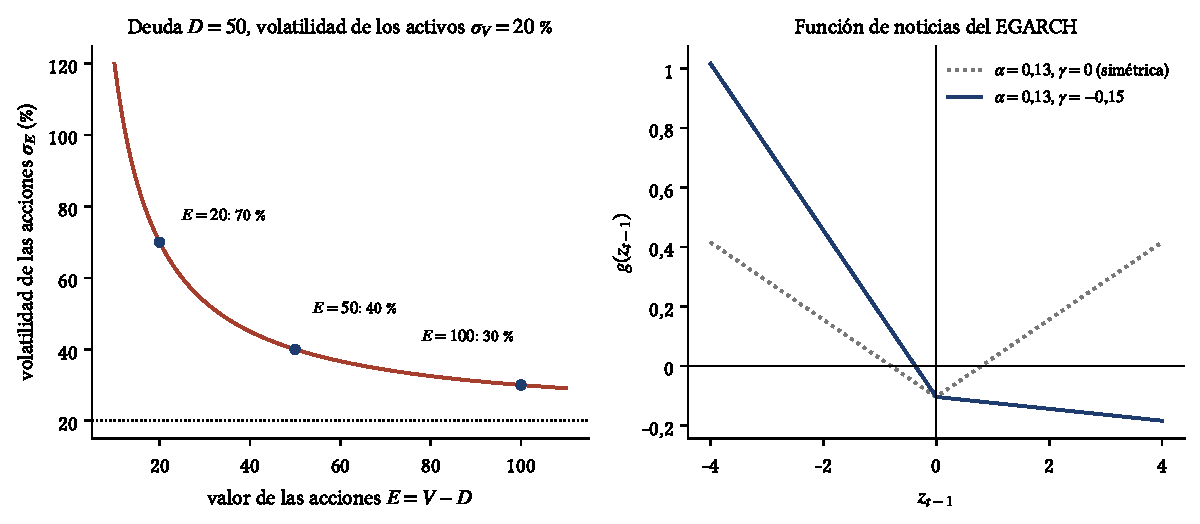
\includegraphics[width=\linewidth]{graficos/cap09_fig_apalancamiento.pdf}
\caption{Izquierda: volatilidad de las acciones según la Proposición~\ref{prop:black} cuando cae el valor de la
empresa; la línea punteada es la volatilidad de los activos. Derecha: función de noticias $g(z)$ del EGARCH,
simétrica con $\gamma=0$ y con pendiente mucho mayor para los choques negativos con $\gamma<0$.}
\label{fig:apalanc}
\end{figure}

% ---------------------------------------------------------------------
\section{Modelos GARCH asimétricos}
% ---------------------------------------------------------------------

\subsection{GJR-GARCH}

\begin{definicion}[GJR-GARCH(1,1); Glosten, Jagannathan y Runkle, 1993]
Sea $I_{t-1}=1$ si $\varepsilon_{t-1}<0$ e $I_{t-1}=0$ en otro caso.
\[
  \sigma_t^2=\omega+\bigl(\alpha+\gamma\,I_{t-1}\bigr)\varepsilon_{t-1}^2+\beta\,\sigma_{t-1}^2,
  \qquad \omega>0,\ \alpha\ge0,\ \alpha+\gamma\ge0,\ \beta\ge0 .
\]
\end{definicion}

Una buena noticia ($\varepsilon_{t-1}>0$) entra con coeficiente $\alpha$; una mala, con $\alpha+\gamma$. Si
$\gamma>0$, hay efecto apalancamiento; $\gamma=0$ devuelve el GARCH(1,1).

\begin{proposicion}[Varianza incondicional del GJR-GARCH]\label{prop:gjr}
Si la distribución de $z_t$ es simétrica alrededor de cero y $\alpha+\gamma/2+\beta<1$,
\[
  \bar\sigma^2=\frac{\omega}{1-\alpha-\gamma/2-\beta}.
\]
\end{proposicion}

\begin{proof}
Primero, por la simetría de $z$, la mitad del segundo momento proviene de los valores negativos:
\begin{align*}
  1 &= \E[z^2]\\
    &= \E\bigl[z^2\,\mathbf 1(z<0)\bigr]+\E\bigl[z^2\,\mathbf 1(z>0)\bigr]\\
    &= 2\,\E\bigl[z^2\,\mathbf 1(z<0)\bigr],\\[4pt]
  \E\bigl[z^2\,\mathbf 1(z<0)\bigr] &= \tfrac12 .
\end{align*}
Como $\varepsilon_{t-1}=\sigma_{t-1}z_{t-1}$ e $I_{t-1}=\mathbf 1(z_{t-1}<0)$, con $\sigma_{t-1}$ independiente de
$z_{t-1}$:
\begin{align*}
  \E\bigl[I_{t-1}\varepsilon_{t-1}^2\bigr] &= \E[\sigma_{t-1}^2]\,\E\bigl[z^2\,\mathbf 1(z<0)\bigr]\\
                                          &= \tfrac12\,\bar\sigma^2 .
\end{align*}
Tomamos esperanzas en la ecuación del modelo:
\begin{align*}
  \bar\sigma^2 &= \omega+\alpha\bar\sigma^2+\gamma\cdot\tfrac12\bar\sigma^2+\beta\bar\sigma^2,\\
  \bar\sigma^2\bigl(1-\alpha-\tfrac\gamma2-\beta\bigr) &= \omega,\\
  \bar\sigma^2 &= \frac{\omega}{1-\alpha-\gamma/2-\beta}. && \qedhere
\end{align*}
\end{proof}

La persistencia del GJR es $\alpha+\gamma/2+\beta$: el término asimétrico cuenta la mitad porque solo actúa la
mitad de las veces. Su pronóstico tiene la misma forma que el de la Proposición~\ref{prop:garchpron}, con esa
persistencia en lugar de $\alpha+\beta$.

\subsection{EGARCH}

\begin{definicion}[EGARCH(1,1); Nelson, 1991]
Con $z_{t-1}=\varepsilon_{t-1}/\sigma_{t-1}$,
\[
  \ln\sigma_t^2=\omega+g(z_{t-1})+\beta\ln\sigma_{t-1}^2,\qquad
  g(z)=\alpha\bigl(|z|-\E|z|\bigr)+\gamma\,z .
\]
\end{definicion}

El modelo tiene tres ventajas. Como se modela el logaritmo, $\sigma_t^2=e^{\ln\sigma_t^2}$ es siempre positiva
y no hacen falta restricciones de signo. La función $g$ es lineal por tramos (Figura~\ref{fig:apalanc},
derecha): su pendiente es $\alpha+\gamma$ para $z>0$ y $\gamma-\alpha$ para $z<0$, de modo que con $\gamma<0$ los
choques negativos pesan más. Y los choques entran estandarizados, en unidades de desviación estándar.

\begin{proposicion}[Media de $|z|$ y estacionariedad del EGARCH]\label{prop:egarch}
En el EGARCH(1,1):
\begin{enumerate}[label=(\roman*)]
  \item Si $z\sim N(0,1)$, $\E|z|=\sqrt{2/\pi}\approx0{,}7979$, de modo que $\E[g(z)]=0$.
  \item Si $|\beta|<1$, el logaritmo $\ln\sigma_t^2$ sigue un AR(1) estacionario, cuya media es
        $\omega/(1-\beta)$.
\end{enumerate}
\end{proposicion}

\begin{proof}
(i) Por simetría, $\E|z|$ es el doble de la integral sobre los positivos. Como
$\frac{d}{dz}\bigl(-e^{-z^2/2}\bigr)=z\,e^{-z^2/2}$,
\begin{align*}
  \E|z| &= 2\int_0^\infty z\,\frac{1}{\sqrt{2\pi}}e^{-z^2/2}\,dz\\
        &= \frac{2}{\sqrt{2\pi}}\Bigl[-e^{-z^2/2}\Bigr]_0^\infty\\
        &= \frac{2}{\sqrt{2\pi}}\,(0+1)\\
        &= \sqrt{\frac{2}{\pi}} .
\end{align*}
Entonces
\begin{align*}
  \E[g(z)] &= \alpha\bigl(\E|z|-\E|z|\bigr)+\gamma\,\E[z]\\
           &= 0+0\\
           &= 0 .
\end{align*}
(ii) Con $y_t=\ln\sigma_t^2$ y $u_t=g(z_{t-1})$, que son i.i.d.\ con media cero, la ecuación es
$y_t=\omega+\beta y_{t-1}+u_t$, un AR(1). Si $|\beta|<1$ es estacionario y, tomando esperanzas,
\begin{align*}
  \E[y] &= \omega+\beta\,\E[y],\\
  \E[y] &= \frac{\omega}{1-\beta}. && \qedhere
\end{align*}
\end{proof}

En el EGARCH la persistencia es $\beta$ y se refiere al logaritmo de la varianza. Si las innovaciones son $t$
de Student, $\E|z|$ ya no es $\sqrt{2/\pi}$; la biblioteca \texttt{arch} y nuestras funciones conservan
$\sqrt{2/\pi}$ como constante de centrado, lo que solo cambia el valor de $\omega$.

\subsection{Curvas de impacto de noticias}

Engle y Ng (1993) propusieron comparar modelos mediante su \emph{curva de impacto de noticias}: la varianza de
mañana, $\sigma_t^2$, como función del choque de hoy, $\varepsilon_{t-1}$, manteniendo fija la varianza de hoy
$\sigma_{t-1}^2$ en un valor típico. La Figura~\ref{fig:nicteo} compara las tres formas con parámetros que dan la
misma persistencia: el GARCH es una parábola simétrica; el GJR, una parábola con dos ramas de distinta
curvatura que se unen en cero; el EGARCH, una curva exponencial asimétrica que crece más despacio para los
choques extremos.

\begin{figure}[ht]
\centering
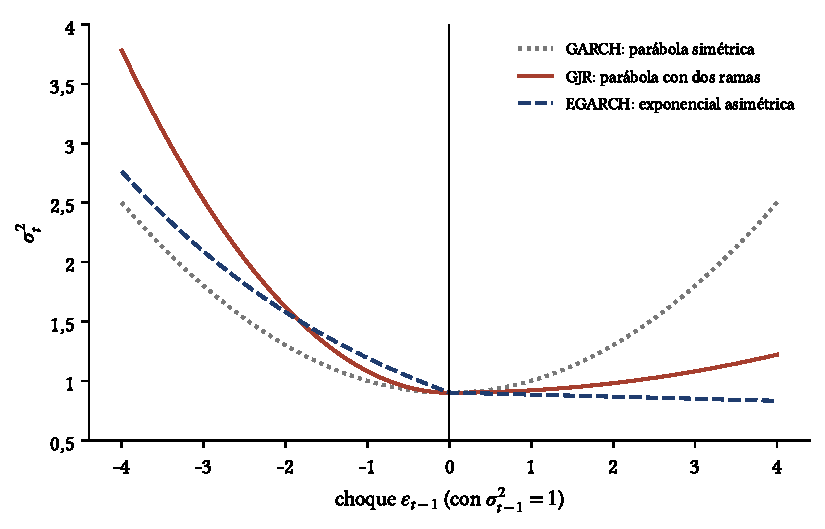
\includegraphics[width=0.72\linewidth]{graficos/cap09_fig_nic_teoria.pdf}
\caption{Curvas de impacto de noticias teóricas con $\sigma_{t-1}^2=1$. GARCH: $\omega=0{,}02$, $\alpha=0{,}10$,
$\beta=0{,}88$. GJR: $\omega=0{,}02$, $\alpha=0{,}02$, $\gamma=0{,}16$, $\beta=0{,}88$. EGARCH: $\omega=0$,
$\alpha=0{,}13$, $\gamma=-0{,}15$, $\beta=0{,}98$.}
\label{fig:nicteo}
\end{figure}

% ---------------------------------------------------------------------
\section{Pruebas de sesgo de signo}
% ---------------------------------------------------------------------

¿Cómo saber si un modelo simétrico deja sin capturar alguna asimetría? Engle y Ng (1993) proponen estimar un
modelo simétrico, calcular los residuos estandarizados $\hat z_t$ y estimar por MCO
\[
  \hat z_t^2=b_0+b_1S^-_{t-1}+b_2S^-_{t-1}\hat z_{t-1}+b_3S^+_{t-1}\hat z_{t-1}+u_t,
\]
donde $S^-_{t-1}=1$ si $\hat z_{t-1}<0$ y $S^+_{t-1}=1-S^-_{t-1}$. Si el modelo es correcto, $\hat z_t^2$ no
debería depender del pasado y los tres coeficientes deberían ser cero:
\begin{itemize}[leftmargin=*]
  \item $b_1$ (\emph{sesgo de signo}): ¿los choques negativos, sin importar su tamaño, elevan la volatilidad más
        de lo que predice el modelo?
  \item $b_2$ (\emph{sesgo de tamaño negativo}): ¿los choques negativos grandes la elevan más que los pequeños?
  \item $b_3$ (\emph{sesgo de tamaño positivo}): lo mismo para los choques positivos.
\end{itemize}
La prueba conjunta usa $LM=(T-1)R^2\xrightarrow{d}\chi^2_3$, con $T-1$ observaciones en la regresión.

% ---------------------------------------------------------------------
\section{GARCH en media: riesgo y rendimiento}
% ---------------------------------------------------------------------

La teoría de carteras dice que los inversionistas aversos al riesgo exigen un premio por soportarlo. Merton
(1980) muestra que, en un modelo de equilibrio intertemporal sencillo, el exceso de rendimiento esperado del
mercado es proporcional a su varianza condicional,
\[
  \E_{t-1}\bigl[r^e_t\bigr]=A\,\sigma_t^2,
\]
donde $A$ es el coeficiente de aversión relativa al riesgo del inversionista representativo. Engle, Lilien y
Robins (1987) propusieron llevar esa idea a la ecuación de la media de un GARCH.

\begin{definicion}[GARCH en media]
\[
  r^e_t=\mu+\lambda\,\sigma_t^2+\varepsilon_t,\qquad \varepsilon_t=\sigma_tz_t,\qquad
  \sigma_t^2=\omega+\alpha\varepsilon_{t-1}^2+\beta\sigma_{t-1}^2 .
\]
\end{definicion}

El modelo de Merton predice $\mu=0$ y $\lambda=A>0$. Hay que cuidar las unidades: si los rendimientos se miden
en porcentaje, $\tilde r^e=100\,r^e$ y $\tilde\sigma^2=10^4\sigma^2$, y la ecuación $\tilde r^e=\lambda\,\tilde\sigma^2$
equivale a
\begin{align*}
  100\,r^e &= \lambda\cdot10^4\,\sigma^2,\\
  r^e      &= 100\,\lambda\,\sigma^2,
\end{align*}
de modo que la aversión al riesgo implícita es $A=100\,\lambda$. La estimación es delicada: la media de los
rendimientos se estima con mucha imprecisión (Capítulo~\ref{cap:rendimientos}), y $\lambda$ aún más. Además, en
este modelo los errores en la ecuación de la varianza contaminan la de la media, porque ambas se estiman a la
vez. Las funciones del capítulo permiten estimar el GARCH-M, el GJR-M y el EGARCH-M con la misma recursión: la
innovación es $\varepsilon_t=r_t-\mu-\lambda\sigma_t^2$, y $\sigma_t^2$ depende de $\varepsilon_{t-1}$.

% ---------------------------------------------------------------------
\section{Ejercicios resueltos}
% ---------------------------------------------------------------------

\begin{ejresuelto}{¿Hay asimetría en el S\&P 500 y en el Brent?}\label{ej:asim}
\enunciado Para los rendimientos diarios del S\&P 500 (1999--2018) y del Brent (1987--2026): (a) calcule
$\operatorname{corr}(r_{t-j},r_t^2)$ y $\operatorname{corr}(r_{t-j}^2,r_t)$ para $j=1,\dots,10$; (b) estime un
GARCH(1,1) normal y aplique las pruebas de sesgo de signo de Engle y Ng a sus residuos estandarizados.

\solucion
\paso{Paso 1. Correlaciones cruzadas.} En el S\&P 500 las correlaciones entre el rendimiento pasado y la
volatilidad presente son negativas en los diez rezagos, entre $-0{,}113$ y $-0{,}036$, todas fuera de la
banda $\pm1{,}96/\sqrt{5\,030}=\pm0{,}028$: los días de caída anuncian días de más volatilidad durante dos
semanas. Las correlaciones en sentido contrario, $\operatorname{corr}(r_{t-j}^2,r_t)$, son pequeñas y de signo
cambiante (Figura~\ref{fig:asim}). El Brent también muestra una correlación negativa en $j=1$ ($-0{,}117$), pero
las siguientes son pequeñas; su $\operatorname{corr}(r_{t-1}^2,r_t)=0{,}123$ es positiva y refleja sobre todo el
rebote del 22 de abril de 2020 después de la caída del día anterior.

\paso{Paso 2. Pruebas de Engle y Ng.}
\begin{center}\small
\begin{tabular}{@{}lrrrr@{}}
\toprule
 & \multicolumn{2}{c}{S\&P 500} & \multicolumn{2}{c}{Brent} \\
\cmidrule(lr){2-3}\cmidrule(lr){4-5}
Coeficiente & Estimación & $t$ & Estimación & $t$ \\
\midrule
$b_0$ constante             & 0,9942 & 16,18 & 0,9809 & 20,79 \\
$b_1$ sesgo de signo        & 0,1733 & 2,06 & 0,0967 & 1,47 \\
$b_2$ tamaño negativo       & 0,0353 & 0,66 & $-0{,}0005$ & $-0{,}01$ \\
$b_3$ tamaño positivo       & $-0{,}1891$ & $-2{,}82$ & $-0{,}0816$ & $-1{,}67$ \\
\midrule
$LM=(T-1)R^2$               & \multicolumn{2}{r}{34,09 ($p=1{,}9\times10^{-7}$)} & \multicolumn{2}{r}{15,36 ($p=0{,}0015$)} \\
\bottomrule
\end{tabular}
\end{center}
Con 3 grados de libertad, el valor crítico al 5\,\% es $7{,}81$: las dos series rechazan que el GARCH simétrico
sea suficiente. En el S\&P 500 el mensaje es claro: después de un choque negativo, $\hat z_t^2$ es en promedio
$0{,}17$ mayor de lo que el GARCH predice ($b_1$), y después de un choque positivo grande es menor ($b_3<0$). El
GARCH simétrico subestima la volatilidad tras las malas noticias y la sobrestima tras las buenas. En el Brent los
coeficientes tienen los mismos signos pero son menores e individualmente no significativos.

\codigoweb{cap09_ej01}
\salidaR{cap09_ej01_R.txt}
\lectura{cap09_ej01}

\RvsPy Las funciones de este capítulo generalizan las del Capítulo~\ref{cap:garch}: una sola recursión cubre el
GARCH, el GJR y el EGARCH, con o sin término en media, y la verosimilitud normal o $t$. Después del
optimizador (\texttt{nlminb} en R, \texttt{L-BFGS-B} en Python) se hacen pasos de Newton con reducción del paso
para afinar el máximo en los dos lenguajes por igual. Ambas funciones devuelven un valor muy grande si unos
parámetros de prueba hacen explotar la recursión, para que el optimizador los descarte. Las diferencias de
espacios en las salidas se deben a que \texttt{sprintf} de R cuenta bytes y la ``ñ'' ocupa dos.

\begin{figure}[ht]
\centering
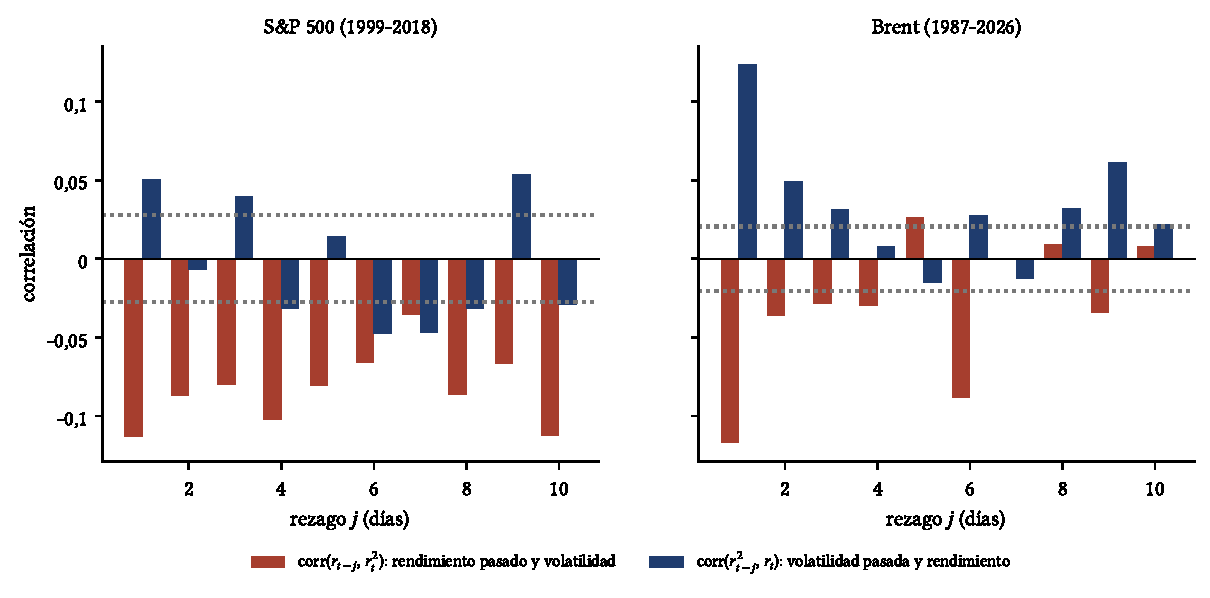
\includegraphics[width=\linewidth]{graficos/cap09_ej01_asimetria.pdf}
\caption{Correlaciones cruzadas entre rendimientos y rendimientos al cuadrado. En el S\&P 500 los rendimientos
pasados se correlacionan negativamente con la volatilidad presente durante al menos diez días.}
\label{fig:asim}
\end{figure}

\begin{conclusion}
El S\&P 500 tiene una asimetría marcada que el GARCH simétrico no captura. En el Brent la asimetría existe, pero
es mucho más débil.
\end{conclusion}
\end{ejresuelto}

\begin{ejresuelto}{GJR-GARCH para el S\&P 500 y comparación con el VIX}\label{ej:gjr}
\enunciado Estime un GJR-GARCH(1,1) con innovaciones $t$ para el S\&P 500 diario. Contraste $\gamma=0$ con una
prueba de razón de verosimilitudes frente al GARCH-$t$. Calcule la persistencia, la vida media y la volatilidad
incondicional. Compare la volatilidad anualizada estimada con el VIX.

\solucion
\paso{Paso 1. Estimación.}
\begin{center}\small
\begin{tabular}{@{}lrrr@{}}
\toprule
 & Coeficiente & ee robusto & $t$ \\
\midrule
$\mu$    & 0,0367 & 0,0104 & 3,52 \\
$\omega$ & 0,0132 & 0,0029 & 4,47 \\
$\alpha$ & 0,0000 & 0,0097 & 0,00 \\
$\gamma$ & 0,1815 & 0,0224 & 8,10 \\
$\beta$  & 0,8987 & 0,0132 & 68,06 \\
$\nu$    & 7,5042 & 0,8352 & 8,99 \\
\bottomrule
\end{tabular}
\end{center}
El resultado es extremo: $\hat\alpha$ llega a su cota de cero. Las buenas noticias no elevan en absoluto la
volatilidad del S\&P 500; solo las malas lo hacen, con coeficiente $\hat\alpha+\hat\gamma=0{,}1815$. (Cuando un
parámetro cae en la frontera, su error estándar y su $t$ no tienen la interpretación habitual.)

\paso{Paso 2. Razón de verosimilitudes.} El GARCH-$t$ simétrico tiene $\hat\ell=-6\,834{,}48$ y el GJR-$t$,
$\hat\ell=-6\,748{,}27$:
\begin{align*}
  LR &= 2\bigl(\hat\ell_{\text{GJR}}-\hat\ell_{\text{GARCH}}\bigr)\\
     &= 2\bigl(-6\,748{,}27+6\,834{,}48\bigr)\\
     &= 2\times86{,}21\\
     &= 172{,}42,
\end{align*}
frente a un valor crítico $\chi^2_1$ al 5\,\% de $3{,}84$ ($p\approx2\times10^{-39}$).

\paso{Paso 3. Persistencia y nivel de largo plazo.} Por la Proposición~\ref{prop:gjr}:
\begin{align*}
  \hat\phi &= \hat\alpha+\frac{\hat\gamma}2+\hat\beta\\
           &= 0+0{,}0907+0{,}8987\\
           &= 0{,}98944,\\[4pt]
  h_{1/2}  &= \frac{\ln0{,}5}{\ln0{,}98944}=65{,}3\ \text{días},\\[4pt]
  \hat{\bar\sigma}^2 &= \frac{0{,}0132}{1-0{,}98944}=1{,}2456 .
\end{align*}
La volatilidad anual de largo plazo es $\sqrt{252\times1{,}2456}=17{,}7$\,\%, algo menor que la muestral, de
19,1\,\%. La persistencia del S\&P 500 es claramente menor que la del Brent: sus choques se disipan en semanas,
no en trimestres.

\paso{Paso 4. Comparación con el VIX.} En los 5\,029 días comunes, la correlación entre la volatilidad
anualizada del GJR y el VIX es $0{,}900$. Pero el VIX es en promedio 3,04 puntos mayor (19,94 frente a 16,89).
La diferencia es la \emph{prima por riesgo de varianza}: los compradores de opciones pagan por protegerse de
aumentos de volatilidad, y la volatilidad implícita en los precios de las opciones supera en promedio a la que
luego se realiza (Figura~\ref{fig:gjrvix}).

\codigoweb{cap09_ej02}
\salidaR{cap09_ej02_R.txt}
\lectura{cap09_ej02}

\RvsPy Las dos implementaciones coinciden con \texttt{arch} en los coeficientes; $\hat\nu$ difiere en la cuarta
cifra decimal entre R ($7{,}5042$) y Python ($7{,}5041$) porque la verosimilitud es muy plana en esa dirección y
porque $\hat\alpha$ en la frontera impide el paso de Newton completo. Para cruzar las fechas con el VIX, R usa
\texttt{match} y Python \texttt{merge}.

\begin{figure}[ht]
\centering
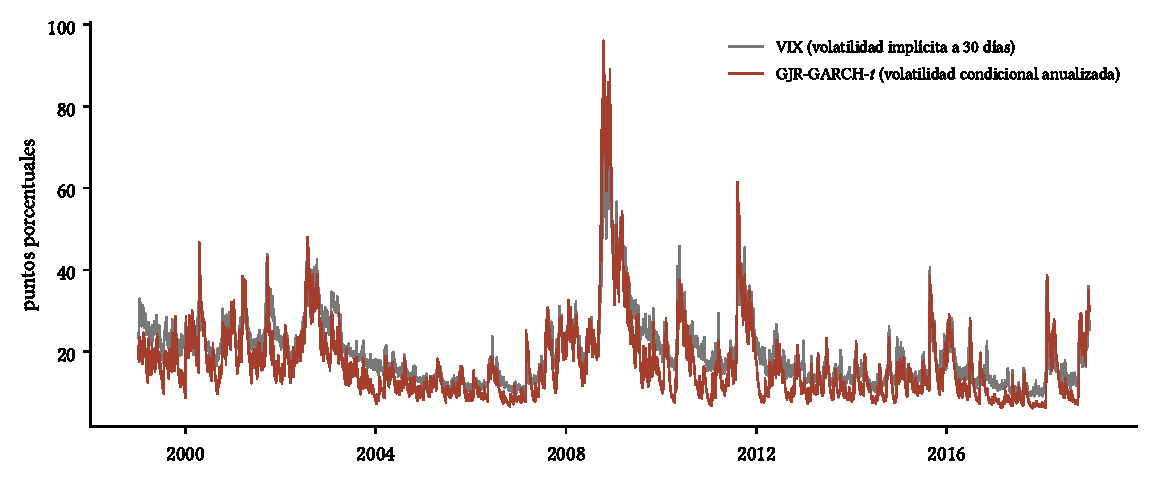
\includegraphics[width=0.92\linewidth]{graficos/cap09_ej02_gjr_vix.pdf}
\caption{Volatilidad condicional anualizada del S\&P 500 según el GJR-GARCH-$t$ y el VIX (1999--2018). Se mueven
juntas, pero el VIX suele estar por encima: es la prima por riesgo de varianza.}
\label{fig:gjrvix}
\end{figure}

\begin{conclusion}
En el S\&P 500 la volatilidad responde casi solo a las malas noticias. El GJR-GARCH mejora la verosimilitud en
86 puntos con un solo parámetro adicional y produce una volatilidad muy parecida a la que el mercado de opciones
incorpora en el VIX.
\end{conclusion}
\end{ejresuelto}

\begin{ejresuelto}{EGARCH y curvas de impacto de noticias del S\&P 500}\label{ej:egarch}
\enunciado Estime un EGARCH(1,1)-$t$ para el S\&P 500. Compare GARCH-$t$, GJR-$t$ y EGARCH-$t$ con AIC y BIC.
Dibuje sus curvas de impacto de noticias con $\sigma_{t-1}^2$ igual a la varianza muestral y calcule, para cada
modelo, el cociente entre la varianza que sigue a un choque de $-2$ y de $+2$ desviaciones estándar.

\solucion
\paso{Paso 1. Estimación.} $\hat\mu=0{,}0367$, $\hat\omega=-0{,}0021$, $\hat\alpha=0{,}1285$ ($t=8{,}96$),
$\hat\gamma=-0{,}1541$ ($t=-11{,}49$), $\hat\beta=0{,}9824$ y $\hat\nu=7{,}29$. Las pendientes de $g(z)$ son
\begin{align*}
  z>0:&\quad \hat\alpha+\hat\gamma=0{,}1285-0{,}1541=-0{,}0256,\\
  z<0:&\quad \hat\gamma-\hat\alpha=-0{,}1541-0{,}1285=-0{,}2826 .
\end{align*}
Para $z<0$, una pendiente negativa significa que la varianza \emph{sube} cuando $z$ se hace más negativo: un
choque de $-1$ eleva $\ln\sigma_t^2$ en $0{,}28$. Para $z>0$, la pendiente es casi nula y ligeramente negativa:
las buenas noticias \emph{reducen} un poco la volatilidad. La vida media de una perturbación en
$\ln\sigma^2$ es $\ln0{,}5/\ln0{,}9824=39{,}1$ días.

\paso{Paso 2. Comparación de modelos.}
\begin{center}\small
\begin{tabular}{@{}lrrrr@{}}
\toprule
Modelo & $k$ & $\hat\ell$ & AIC & BIC \\
\midrule
GARCH-$t$  & 5 & $-6\,834{,}48$ & 13\,678,96 & 13\,711,57 \\
GJR-$t$    & 6 & $-6\,748{,}27$ & 13\,508,54 & 13\,547,68 \\
EGARCH-$t$ & 6 & $-6\,732{,}24$ & 13\,476,49 & 13\,515,63 \\
\bottomrule
\end{tabular}
\end{center}
Los dos criterios eligen el EGARCH, con el mismo número de parámetros que el GJR y 16 puntos más de
log-verosimilitud. Los dos modelos asimétricos superan con holgura al simétrico.

\paso{Paso 3. Curvas de impacto.} Con $\sigma_{t-1}^2=1{,}4492$, un choque de dos desviaciones estándar es
$2\sqrt{1{,}4492}=2{,}408$\,\%. La varianza de mañana resulta:
\begin{center}\small
\begin{tabular}{@{}lrrr@{}}
\toprule
Modelo & $\sigma_t^2$ tras $-2{,}408$\,\% & $\sigma_t^2$ tras $+2{,}408$\,\% & Cociente \\
\midrule
GARCH-$t$  & 1,8899 & 1,8899 & 1,00 \\
GJR-$t$    & 2,3676 & 1,3156 & 1,80 \\
EGARCH-$t$ & 2,2820 & 1,2321 & 1,85 \\
\bottomrule
\end{tabular}
\end{center}
En el GJR, por ejemplo,
\begin{align*}
  \sigma_t^2(-) &= 0{,}0132+0{,}1815\times2{,}408^2+0{,}8987\times1{,}4492 = 2{,}3676,\\
  \sigma_t^2(+) &= 0{,}0132+0\times2{,}408^2+0{,}8987\times1{,}4492 = 1{,}3156 .
\end{align*}
Una caída de dos desviaciones estándar lleva la varianza de mañana a casi el doble que una subida del mismo
tamaño. La Figura~\ref{fig:nicsp} muestra las curvas completas: el GARCH simétrico sobrestima la reacción a las
subidas y subestima la reacción a las caídas.

\codigoweb{cap09_ej03}
\salidaR{cap09_ej03_R.txt}
\lectura{cap09_ej03}

\RvsPy Las tres implementaciones (R, Python y \texttt{arch}) coinciden. La curva de impacto del EGARCH se
programa con la misma ecuación de la recursión, con $z_{t-1}=\varepsilon_{t-1}/\sigma_{t-1}$.

\begin{figure}[ht]
\centering
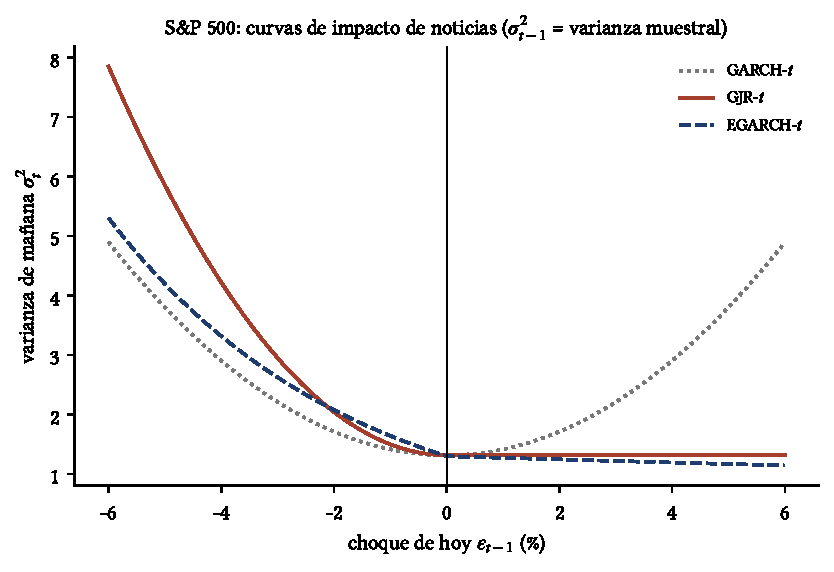
\includegraphics[width=0.74\linewidth]{graficos/cap09_ej03_nic_sp500.pdf}
\caption{Curvas de impacto de noticias estimadas para el S\&P 500. La rama derecha del GJR es plana porque
$\hat\alpha=0$; la del EGARCH desciende levemente porque $\hat\alpha+\hat\gamma<0$.}
\label{fig:nicsp}
\end{figure}

\begin{conclusion}
Los modelos asimétricos describen mucho mejor la volatilidad de las acciones. El EGARCH, que trabaja con
logaritmos y choques estandarizados, es el preferido por los criterios de información en esta muestra.
\end{conclusion}
\end{ejresuelto}

\begin{ejresuelto}{¿Tiene el petróleo efecto apalancamiento?}\label{ej:asimbrent}
\enunciado Estime GARCH-$t$, GJR-$t$ y EGARCH-$t$ para el Brent. Contraste $\gamma=0$ en el GJR. Calcule el
cociente de impactos de choques de $\pm2$ desviaciones estándar y compare con el S\&P 500. Verifique que el
resultado no depende de los episodios extremos de 2020--2026 reestimando el GJR hasta 2019.

\solucion
\paso{Paso 1. GJR-$t$.} $\hat\alpha=0{,}0676$, $\hat\gamma=0{,}0314$ ($t=3{,}09$), $\hat\beta=0{,}9115$ y
$\hat\nu=5{,}27$. La razón de verosimilitudes frente al GARCH-$t$ es
\begin{align*}
  LR &= 2\bigl(-19\,747{,}20+19\,752{,}61\bigr)\\
     &= 10{,}81\quad(p=0{,}0010).
\end{align*}
Hay asimetría en el Brent, del mismo signo que en las acciones, y significativa.

\paso{Paso 2. Magnitud.} En el GJR el coeficiente de $\varepsilon_{t-1}^2$ es $0{,}0990$ para las caídas y
$0{,}0676$ para las subidas:
\begin{align*}
  \frac{\hat\alpha+\hat\gamma}{\hat\alpha} &= \frac{0{,}0990}{0{,}0676}\\
                                         &= 1{,}46 .
\end{align*}
En el S\&P 500 ese cociente es infinito ($\hat\alpha=0$). Para un choque de dos desviaciones estándar ($5{,}408$\,\%),
el cociente de varianzas es $1{,}11$ en el GJR y $1{,}13$ en el EGARCH, frente a $1{,}80$ y $1{,}85$ en el
S\&P 500. La Figura~\ref{fig:nicbrent} compara las dos curvas en unidades comparables: la del Brent es casi
simétrica; la del S\&P 500 tiene una sola rama.

\paso{Paso 3. Comparación de modelos.}
\begin{center}\small
\begin{tabular}{@{}lrrrr@{}}
\toprule
Modelo & $k$ & $\hat\ell$ & AIC & BIC \\
\midrule
GARCH-$t$  & 5 & $-19\,752{,}61$ & 39\,515,21 & 39\,550,81 \\
GJR-$t$    & 6 & $-19\,747{,}20$ & 39\,506,40 & 39\,549,11 \\
EGARCH-$t$ & 6 & $-19\,722{,}71$ & 39\,457,42 & 39\,500,13 \\
\bottomrule
\end{tabular}
\end{center}
El EGARCH vuelve a ganar, pero aquí su ventaja no viene de la asimetría ($\hat\gamma=-0{,}0304$ es pequeña),
sino de su forma logarítmica, que responde con menos violencia a los choques enormes del Brent.

\paso{Paso 4. Robustez.} Con datos hasta 2019 ($T=7\,390$), $\hat\gamma=0{,}0301$ ($t=3{,}24$): la asimetría es
la misma sin la pandemia ni el año 2026.

\codigoweb{cap09_ej04}
\salidaR{cap09_ej04_R.txt}
\lectura{cap09_ej04}

\RvsPy En el EGARCH del Brent, R y Python se detienen en puntos que difieren en la cuarta decimal de $\hat\mu$
($0{,}0384$ frente a $0{,}0385$), con log-verosimilitudes que difieren en $0{,}00001$. La verosimilitud del EGARCH
no es derivable en todos los puntos (contiene $|z_{t-1}|$, y $z_{t-1}$ depende de $\mu$) y es casi plana en esa
dirección, así que el paso de Newton no puede afinar más; la diferencia no tiene ninguna consecuencia práctica.

\begin{figure}[ht]
\centering
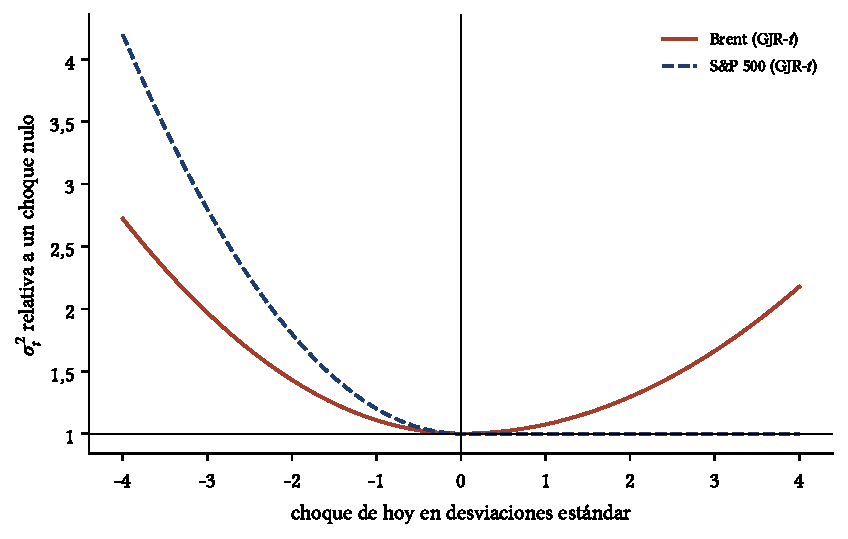
\includegraphics[width=0.74\linewidth]{graficos/cap09_ej04_nic_brent.pdf}
\caption{Curvas de impacto del GJR-$t$ en unidades de desviación estándar, relativas a la varianza tras un choque
nulo. El Brent responde de forma casi simétrica; el S\&P 500 solo a las caídas.}
\label{fig:nicbrent}
\end{figure}

\begin{conclusion}
El Brent tiene un efecto apalancamiento estadísticamente significativo, pero pequeño. Tiene sentido: en el
petróleo, las subidas bruscas del precio (por ejemplo, ante interrupciones de la oferta) también son noticias
que generan incertidumbre, mientras que la explicación por apalancamiento financiero no se aplica a una materia
prima.
\end{conclusion}
\end{ejresuelto}

\begin{ejresuelto}{GARCH en media: ¿pagan más las acciones cuando son más riesgosas?}\label{ej:garchm}
\enunciado Con el exceso de rendimiento mensual del mercado de EE.\,UU. (1926--2018, en porcentaje), estime un
GARCH-M con innovaciones normales y $t$, y un GJR-M con innovaciones $t$. Contraste $\lambda=0$, calcule la prima
implícita para la varianza promedio e interprete $\lambda$ como aversión al riesgo.

\solucion
\paso{Paso 1. Estimaciones.} Con $T=1\,109$ meses (media $0{,}66$\,\% mensual, varianza $28{,}38$):
\begin{center}\small
\begin{tabular}{@{}lrrrrr@{}}
\toprule
Modelo & $\hat\lambda$ & ee robusto & $t$ & Prima anual & $A=100\hat\lambda$ \\
\midrule
GARCH-M normal & 0,01167 & 0,00877 & 1,33 & 4,07\,\% & 1,17 \\
GARCH-M $t$    & 0,00872 & 0,00881 & 0,99 & 2,95\,\% & 0,87 \\
GJR-M $t$      & 0,00408 & 0,01115 & 0,37 & 1,34\,\% & 0,41 \\
\bottomrule
\end{tabular}
\end{center}
La prima es $\hat\lambda$ por la varianza condicional promedio, multiplicada por 12. Para el GARCH-M normal,
$0{,}3390\times12=4{,}07$\,\%.

\paso{Paso 2. Interpretación.} Los tres $\hat\lambda$ son positivos, como predice la teoría, y las aversiones
al riesgo implícitas (entre 0,4 y 1,2) son razonables. Pero ninguno es significativo, y la estimación cae a la
mitad o menos cuando se permite la asimetría. Es el resultado que encontraron Glosten, Jagannathan y Runkle
(1993): una vez que se modela que las caídas elevan la volatilidad, la relación positiva entre varianza y
rendimiento esperado se debilita o desaparece. En el GARCH-M simétrico, parte de $\hat\lambda$ captura
sencillamente que los meses de varianza alta suelen seguir a rebotes.

\paso{Paso 3. La prima en el tiempo.} Según el GARCH-M $t$, el exceso esperado anualizado
$12(\hat\mu+\hat\lambda\hat\sigma_t^2)$ llegó a casi 50\,\% en septiembre de 1932, cuando la volatilidad anualizada
alcanzó 68\,\%
(Figura~\ref{fig:garchm}). Ese tipo de predicciones extremas es otra razón para desconfiar de una relación lineal
entre la varianza y la media.

\codigoweb{cap09_ej05}
\salidaR{cap09_ej05_R.txt}
\lectura{cap09_ej05}

\RvsPy El GARCH-M se estima con las mismas funciones, indicando \texttt{media = "m"}. Acotamos $\lambda$ entre
$-0{,}5$ y $0{,}5$: sin cota, durante la búsqueda el optimizador de Python probaba valores que hacían explotar la
recursión. \texttt{arch} no incluye el GARCH en media, así que la verificación es entre R y Python, que coinciden
en todas las cifras.

\begin{figure}[ht]
\centering
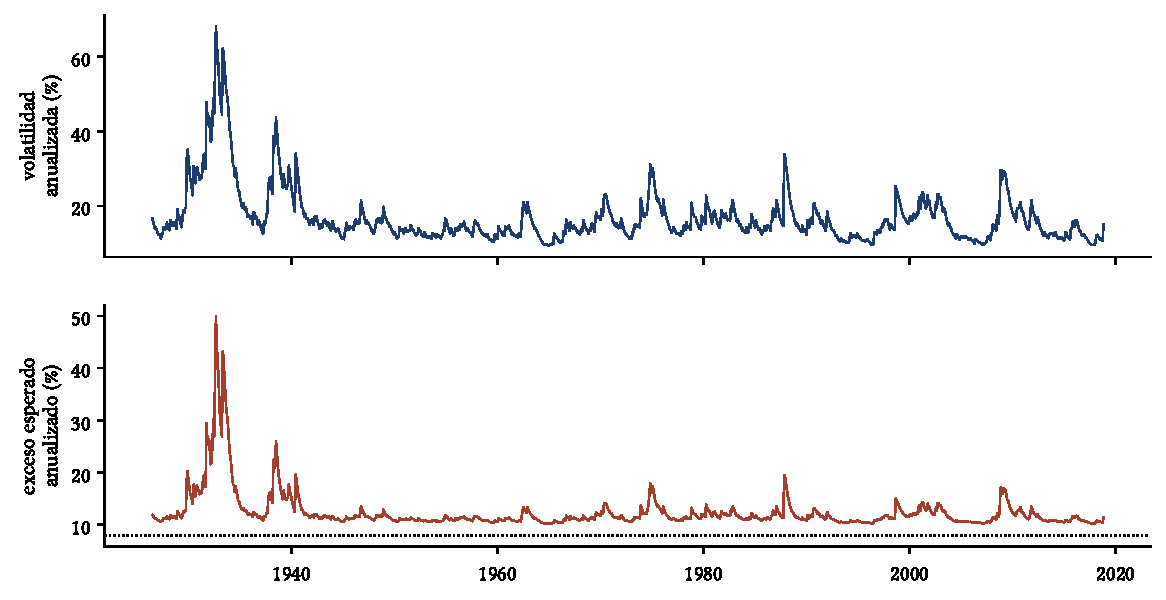
\includegraphics[width=0.92\linewidth]{graficos/cap09_ej05_garch_m.pdf}
\caption{GARCH-M $t$ para el exceso de rendimiento del mercado (1926--2018). Arriba: volatilidad condicional
anualizada. Abajo: exceso de rendimiento esperado anualizado; la línea punteada es el promedio muestral.}
\label{fig:garchm}
\end{figure}

\begin{conclusion}
Los datos son compatibles con una relación positiva entre riesgo y rendimiento esperado, pero no permiten
establecerla con confianza. La relación riesgo-rendimiento en el tiempo sigue siendo una de las preguntas
abiertas de la econometría financiera.
\end{conclusion}
\end{ejresuelto}

% ---------------------------------------------------------------------
\section{Ejercicios propuestos}
% ---------------------------------------------------------------------

\begin{enumerate}[label=\textbf{\thechapter.\arabic*},leftmargin=*,itemsep=6pt]
  \item Para un GJR-GARCH con $\omega=0{,}02$, $\alpha=0{,}03$, $\gamma=0{,}10$ y $\beta=0{,}90$, calcule la
  persistencia, la varianza incondicional y la vida media. \textit{Respuesta: $0{,}98$; $1$; $34{,}3$ períodos.}

  \item En un EGARCH con $\alpha=0{,}13$ y $\gamma=-0{,}15$ e innovaciones normales, calcule $g(2)$ y $g(-2)$, y el
  cociente $e^{g(-2)}/e^{g(2)}$. \textit{Respuesta: $-0{,}1437$; $0{,}4563$; $1{,}822$.}

  \item Una empresa tiene activos de 150, deuda sin riesgo de 60 y volatilidad de activos de 15\,\%. Calcule la
  volatilidad de sus acciones antes y después de que los activos caigan a 100. \textit{Respuesta: 25\,\% y
  37,5\,\%.}

  \item Demuestre que, para la $t$ estandarizada con $\nu$ grados de libertad,
  \[
    \E|z|=\frac{2\sqrt{\nu-2}\;\Gamma\bigl(\frac{\nu+1}2\bigr)}{\sqrt\pi\,(\nu-1)\,\Gamma\bigl(\frac\nu2\bigr)} .
  \]
  Evalúela en $\nu=7{,}2855$ y compárela con $\sqrt{2/\pi}$. \textit{Respuesta: $0{,}7612$ frente a $0{,}7979$.}

  \item Demuestre que en el GJR-GARCH el pronóstico de la varianza es
  $\E_T[\sigma_{T+h}^2]=\bar\sigma^2+\phi^{h-1}(\sigma_{T+1}^2-\bar\sigma^2)$ con $\phi=\alpha+\gamma/2+\beta$.

  \item \emph{(Simulación.)} Simule 500 muestras de 2\,000 observaciones de un GJR-GARCH normal con los
  parámetros del ejercicio 9.1, estime un GARCH(1,1) simétrico y aplique la prueba conjunta de Engle y Ng. ¿Con
  qué frecuencia detecta la asimetría?

  \item \emph{(Con datos.)} El paquete \texttt{arch} incluye el índice Nasdaq diario de 1999 a 2018
  (\texttt{arch.data.nasdaq}). Estime el GJR-$t$ y el EGARCH-$t$ y compare la asimetría y la persistencia con las
  del S\&P 500.

  \item \emph{(Con datos de Yahoo Finance.)} Descargue el índice S\&P/BVL Perú General y las acciones de
  Southern Copper (SCCO) y Credicorp (BAP). ¿Muestran efecto apalancamiento? ¿Es mayor en el banco, más
  endeudado, que en la minera?
\end{enumerate}

% ---------------------------------------------------------------------
\section{Resumen de fórmulas}
% ---------------------------------------------------------------------

\begin{table}[H]
\centering\small
\begin{tabular}{@{}ll@{}}
\toprule
Concepto & Fórmula \\
\midrule
Apalancamiento & $\sigma_E=(1+D/E)\,\sigma_V$ \\
GJR-GARCH & $\sigma_t^2=\omega+(\alpha+\gamma I_{t-1})\varepsilon_{t-1}^2+\beta\sigma_{t-1}^2$ \\
Persistencia GJR & $\alpha+\gamma/2+\beta$;\quad $\bar\sigma^2=\omega/(1-\alpha-\gamma/2-\beta)$ \\
EGARCH & $\ln\sigma_t^2=\omega+\alpha(|z_{t-1}|-\sqrt{2/\pi})+\gamma z_{t-1}+\beta\ln\sigma_{t-1}^2$ \\
Pendientes de $g(z)$ & $\alpha+\gamma$ si $z>0$;\quad $\gamma-\alpha$ si $z<0$ \\
Engle-Ng & $\hat z_t^2=b_0+b_1S^-_{t-1}+b_2S^-_{t-1}\hat z_{t-1}+b_3S^+_{t-1}\hat z_{t-1}$;\quad $(T-1)R^2\sim\chi^2_3$ \\
GARCH-M & $r^e_t=\mu+\lambda\sigma_t^2+\varepsilon_t$;\quad $A=100\lambda$ (datos en \%) \\
\bottomrule
\end{tabular}
\caption{Fórmulas principales del Capítulo 9.}
\end{table}

\section*{Referencias}
\begin{itemize}[leftmargin=*]
  \item Black, F. (1976). Studies of stock price volatility changes. \emph{Proceedings of the 1976 Meetings of the
        American Statistical Association, Business and Economic Statistics Section}, 177--181.
  \item Campbell, J. Y. y Hentschel, L. (1992). No news is good news: An asymmetric model of changing volatility
        in stock returns. \emph{Journal of Financial Economics}, 31(3), 281--318.
  \item Engle, R. F., Lilien, D. M. y Robins, R. P. (1987). Estimating time varying risk premia in the term
        structure: The ARCH-M model. \emph{Econometrica}, 55(2), 391--407.
  \item Engle, R. F. y Ng, V. K. (1993). Measuring and testing the impact of news on volatility. \emph{Journal
        of Finance}, 48(5), 1749--1778.
  \item Figlewski, S. y Wang, X. (2000). Is the ``leverage effect'' a leverage effect? Documento de trabajo,
        New York University.
  \item Glosten, L. R., Jagannathan, R. y Runkle, D. E. (1993). On the relation between the expected value and
        the volatility of the nominal excess return on stocks. \emph{Journal of Finance}, 48(5), 1779--1801.
  \item Merton, R. C. (1980). On estimating the expected return on the market: An exploratory investigation.
        \emph{Journal of Financial Economics}, 8(4), 323--361.
  \item Nelson, D. B. (1991). Conditional heteroskedasticity in asset returns: A new approach.
        \emph{Econometrica}, 59(2), 347--370.
\end{itemize}

% =====================================================================
%  Capítulo 10. Vectores autorregresivos
% =====================================================================
\part{Modelos multivariados}
\chapter[Vectores autorregresivos]{Vectores autorregresivos: causalidad, impulso-respuesta y pronóstico}\label{cap:var}

\section*{Objetivos de aprendizaje}
Al terminar este capítulo, el lector podrá:
\begin{enumerate}[label=\arabic*.,leftmargin=*]
  \item Escribir un VAR($p$) en forma compañera, verificar su estabilidad con los autovalores y obtener su
        representación de medias móviles.
  \item Demostrar que MCO ecuación por ecuación es eficiente en un VAR y elegir el orden con criterios de
        información.
  \item Contrastar la causalidad de Granger con pruebas clásicas y robustas.
  \item Calcular e interpretar respuestas al impulso ortogonalizadas y la descomposición de la varianza del
        error de pronóstico, y reconocer su dependencia del orden de las variables.
  \item Evaluar fuera de muestra si un VAR pronostica mejor que modelos más simples.
\end{enumerate}

\section*{Motivación}
Hasta ahora hemos modelado una serie a la vez. Pero los precios financieros se mueven juntos y se influyen
mutuamente: cuando el S\&P 500 cae, el VIX sube; cuando sube la tasa de interés, las acciones suelen bajar; las
acciones grandes parecen adelantarse a las pequeñas (Capítulo~\ref{cap:eficiencia}). El \emph{vector
autorregresivo} (VAR), propuesto por Sims (1980) como alternativa a los grandes modelos macroeconómicos, trata
todas las variables como endógenas y deja que los datos digan cómo interactúan. Sus herramientas (la
causalidad de Granger, las respuestas al impulso y la descomposición de la varianza) son hoy el lenguaje común
para estudiar la transmisión de choques entre mercados.

\paragraph{Datos del capítulo.} Rendimientos diarios del S\&P 500 y cambios logarítmicos diarios del VIX
(1999--2018, $T=5\,029$); carteras pequeña (S1V3) y grande (S5V3) de la base de French (1949--2017), y una
muestra mensual de EE.\,UU.\ de la base de Shiller (1960--2023) con la inflación, el cambio en la tasa de los
bonos a 10 años y el rendimiento total del S\&P 500.

% ---------------------------------------------------------------------
\section{El modelo VAR}
% ---------------------------------------------------------------------

\begin{definicion}[VAR($p$)]
Un vector $\mathbf y_t$ de $K$ variables sigue un vector autorregresivo de orden $p$ si
\[
  \mathbf y_t=\mathbf c+A_1\mathbf y_{t-1}+A_2\mathbf y_{t-2}+\dots+A_p\mathbf y_{t-p}+\mathbf u_t,
\]
donde $\mathbf c$ es un vector $K\times1$, cada $A_j$ es una matriz $K\times K$ y $\mathbf u_t$ es un ruido
blanco vectorial: $\E[\mathbf u_t]=\mathbf 0$, $\E[\mathbf u_t\mathbf u_t']=\Sigma$ y
$\E[\mathbf u_t\mathbf u_s']=0$ si $t\ne s$.
\end{definicion}

Cada ecuación es una regresión de una variable sobre $p$ rezagos de todas. Con $K=2$ y $p=1$, por ejemplo:
\begin{align*}
  y_{1t} &= c_1+a_{11}y_{1,t-1}+a_{12}y_{2,t-1}+u_{1t},\\
  y_{2t} &= c_2+a_{21}y_{1,t-1}+a_{22}y_{2,t-1}+u_{2t}.
\end{align*}
El coeficiente $a_{12}$ mide cómo el pasado de $y_2$ ayuda a predecir $y_1$. Las innovaciones $u_{1t}$ y
$u_{2t}$ pueden estar correlacionadas: $\Sigma$ no es diagonal. Esa correlación contemporánea es la que obliga,
más adelante, a decidir un orden entre las variables.

\subsection{Forma compañera y estabilidad}

Un VAR($p$) puede escribirse como un VAR(1) apilando los rezagos. Con
$\boldsymbol\xi_t=(\mathbf y_t',\mathbf y_{t-1}',\dots,\mathbf y_{t-p+1}')'$, de dimensión $Kp$,
\[
  \boldsymbol\xi_t=\boldsymbol\nu+F\,\boldsymbol\xi_{t-1}+\mathbf v_t,\qquad
  F=\begin{bmatrix}
      A_1 & A_2 & \cdots & A_{p-1} & A_p\\
      I_K & 0   & \cdots & 0       & 0\\
      0   & I_K & \cdots & 0       & 0\\
      \vdots &  & \ddots &         & \vdots\\
      0   & 0   & \cdots & I_K     & 0
    \end{bmatrix},
\]
con $\boldsymbol\nu=(\mathbf c',\mathbf 0',\dots)'$ y $\mathbf v_t=(\mathbf u_t',\mathbf 0',\dots)'$. Las filas
inferiores de $F$ solo dicen que $\mathbf y_{t-1}$ es $\mathbf y_{t-1}$. La matriz $F$ es la \emph{matriz
compañera}.

\begin{proposicion}[Estabilidad y representación de medias móviles]\label{prop:varma}
Si todos los autovalores de $F$ tienen módulo menor que uno, el VAR es estacionario y
\[
  \mathbf y_t=\boldsymbol\mu+\sum_{i=0}^{\infty}\Psi_i\,\mathbf u_{t-i},\qquad \Psi_0=I_K,\qquad
  \Psi_i=\sum_{j=1}^{\min(i,p)}A_j\Psi_{i-j}\ \ (i\ge1),
\]
donde $\boldsymbol\mu=(I_K-A_1-\dots-A_p)^{-1}\mathbf c$ es la media del proceso.
\end{proposicion}

\begin{proof}
Trabajamos con la forma compañera, en desviaciones respecto de su media $\bar{\boldsymbol\xi}$:
$\tilde{\boldsymbol\xi}_t=F\tilde{\boldsymbol\xi}_{t-1}+\mathbf v_t$. Sustituimos hacia atrás $k$ veces:
\begin{align*}
  \tilde{\boldsymbol\xi}_t &= F\tilde{\boldsymbol\xi}_{t-1}+\mathbf v_t\\
                           &= F\bigl(F\tilde{\boldsymbol\xi}_{t-2}+\mathbf v_{t-1}\bigr)+\mathbf v_t\\
                           &= F^2\tilde{\boldsymbol\xi}_{t-2}+F\mathbf v_{t-1}+\mathbf v_t\\
                           &\;\;\vdots\\
                           &= F^k\tilde{\boldsymbol\xi}_{t-k}+\sum_{i=0}^{k-1}F^i\mathbf v_{t-i}.
\end{align*}
Si $F=VDV^{-1}$ con $D$ diagonal de autovalores $\lambda_\ell$ (el caso general usa la forma de Jordan con el
mismo resultado), entonces $F^k=VD^kV^{-1}$ y cada elemento de $D^k$ es $\lambda_\ell^k\to0$ porque
$|\lambda_\ell|<1$. Así $F^k\tilde{\boldsymbol\xi}_{t-k}\to0$ y
\begin{align*}
  \tilde{\boldsymbol\xi}_t &= \sum_{i=0}^{\infty}F^i\mathbf v_{t-i}.
\end{align*}
Las primeras $K$ filas dan $\mathbf y_t-\boldsymbol\mu=\sum_i\Psi_i\mathbf u_{t-i}$, con $\Psi_i$ el bloque
superior izquierdo de $F^i$. Para la recursión, sustituimos la representación en el VAR e igualamos los
coeficientes de $\mathbf u_{t-i}$ en ambos lados:
\begin{align*}
  \sum_{i\ge0}\Psi_i\mathbf u_{t-i}
     &= \sum_{j=1}^{p}A_j\sum_{m\ge0}\Psi_m\mathbf u_{t-j-m}+\mathbf u_t,\\
  \text{coeficiente de }\mathbf u_t:\quad \Psi_0 &= I_K,\\
  \text{coeficiente de }\mathbf u_{t-i}:\quad \Psi_i &= \sum_{j=1}^{\min(i,p)}A_j\Psi_{i-j}. && \qedhere
\end{align*}
\end{proof}

La forma de las respuestas depende de los autovalores. Si son reales y menores que uno, los efectos de un
choque decaen de forma monótona; si son complejos, $\lambda=re^{\pm i\theta}$, decaen oscilando, con período
$2\pi/\theta$ y amortiguamiento $r^i$; si alguno tiene módulo mayor que uno, explotan. La
Figura~\ref{fig:varautoval} muestra los tres casos con un VAR(1) bivariado. En el panel izquierdo los
autovalores reales $0{,}5$ de los dos primeros casos coinciden en el mismo punto.

\begin{figure}[ht]
\centering
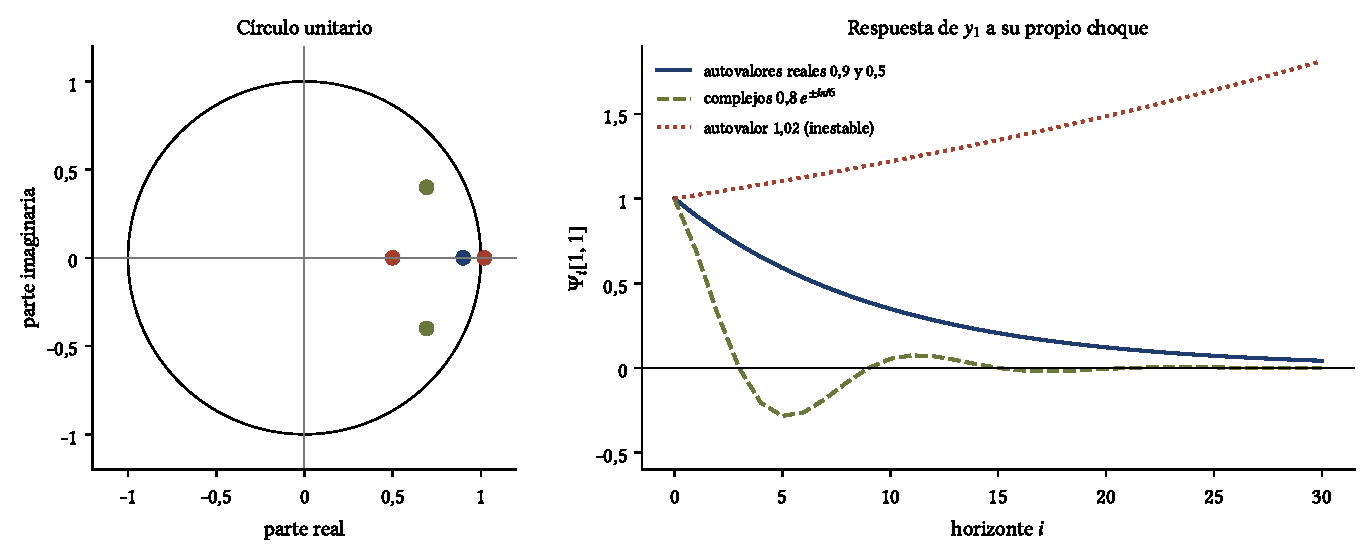
\includegraphics[width=\linewidth]{graficos/cap10_fig_autovalores.pdf}
\caption{Izquierda: autovalores de tres VAR(1) bivariados frente al círculo unitario. Derecha: elemento
$[1,1]$ de $\Psi_i$, la respuesta de $y_1$ a su propia innovación. Autovalores reales dentro del círculo:
decaimiento monótono. Complejos: oscilación amortiguada. Uno fuera del círculo: explosión.}
\label{fig:varautoval}
\end{figure}

% ---------------------------------------------------------------------
\section{Estimación y selección del orden}
% ---------------------------------------------------------------------

Sea $X$ la matriz $n\times(1+Kp)$ cuya fila $t$ es $(1,\mathbf y_{t-1}',\dots,\mathbf y_{t-p}')$ y $Y$ la matriz
$n\times K$ cuya fila $t$ es $\mathbf y_t'$. El VAR se escribe $Y=XB+U$, con
$B=(\mathbf c,A_1,\dots,A_p)'$ de dimensión $(1+Kp)\times K$: cada columna de $B$ contiene los coeficientes de
una ecuación. El estimador de MCO ecuación por ecuación es $\hat B=(X'X)^{-1}X'Y$.

\begin{proposicion}[MCO ecuación por ecuación es MCG]\label{prop:varmco}
Como todas las ecuaciones tienen los mismos regresores, el estimador de mínimos cuadrados generalizados del
sistema, que aprovecha la correlación $\Sigma$ entre ecuaciones, coincide con MCO ecuación por ecuación. Con
errores normales, coincide también con el de máxima verosimilitud.
\end{proposicion}

\begin{proof}
Apilamos las columnas de $Y$ y de $U$ en un solo vector:
$\operatorname{vec}(Y)=(I_K\otimes X)\boldsymbol\beta+\operatorname{vec}(U)$, con
$\boldsymbol\beta=\operatorname{vec}(B)$ y $\Var[\operatorname{vec}(U)]=\Sigma\otimes I_n$. El estimador MCG es
\begin{align*}
  \hat{\boldsymbol\beta}_{\text{MCG}}
    &= \bigl[(I_K\otimes X)'(\Sigma^{-1}\otimes I_n)(I_K\otimes X)\bigr]^{-1}
       (I_K\otimes X)'(\Sigma^{-1}\otimes I_n)\operatorname{vec}(Y).
\end{align*}
Usamos las reglas $(A\otimes B)'=A'\otimes B'$, $(A\otimes B)(C\otimes D)=AC\otimes BD$ y
$(A\otimes B)^{-1}=A^{-1}\otimes B^{-1}$. El término entre corchetes es
\begin{align*}
  (I_K\otimes X')(\Sigma^{-1}\otimes I_n)(I_K\otimes X)
    &= (\Sigma^{-1}\otimes X')(I_K\otimes X)\\
    &= \Sigma^{-1}\otimes X'X,
\end{align*}
y el factor que multiplica a $\operatorname{vec}(Y)$ es
\begin{align*}
  (I_K\otimes X')(\Sigma^{-1}\otimes I_n) &= \Sigma^{-1}\otimes X'.
\end{align*}
Entonces
\begin{align*}
  \hat{\boldsymbol\beta}_{\text{MCG}}
    &= \bigl(\Sigma^{-1}\otimes X'X\bigr)^{-1}\bigl(\Sigma^{-1}\otimes X'\bigr)\operatorname{vec}(Y)\\
    &= \bigl(\Sigma\otimes(X'X)^{-1}\bigr)\bigl(\Sigma^{-1}\otimes X'\bigr)\operatorname{vec}(Y)\\
    &= \bigl(\Sigma\Sigma^{-1}\otimes(X'X)^{-1}X'\bigr)\operatorname{vec}(Y)\\
    &= \bigl(I_K\otimes(X'X)^{-1}X'\bigr)\operatorname{vec}(Y).
\end{align*}
El último operador aplica $(X'X)^{-1}X'$ a cada columna de $Y$, que es MCO ecuación por ecuación. Con errores
normales, maximizar la verosimilitud respecto de $\boldsymbol\beta$ equivale a minimizar la forma cuadrática que
minimiza MCG.
\end{proof}

La matriz de covarianzas de los residuos se estima con $\hat\Sigma=\hat U'\hat U/(n-1-Kp)$, o con $\tilde\Sigma=\hat
U'\hat U/n$ (máxima verosimilitud). El orden $p$ se elige minimizando un criterio de información sobre una
\emph{misma} muestra efectiva para todos los candidatos (se descartan las primeras $p_{\max}$ observaciones):
\begin{align*}
  \text{AIC}(p) &= \ln\bigl|\tilde\Sigma_p\bigr|+\frac{2}{n}\,k,\\
  \text{BIC}(p) &= \ln\bigl|\tilde\Sigma_p\bigr|+\frac{\ln n}{n}\,k,\\
  \text{HQ}(p)  &= \ln\bigl|\tilde\Sigma_p\bigr|+\frac{2\ln\ln n}{n}\,k,
\end{align*}
con $k=pK^2+K$ parámetros. Como en el caso univariado, el BIC penaliza más y elige modelos más parsimoniosos; el
AIC tiende a sobreajustar, pero es preferible si el objetivo es pronosticar.

% ---------------------------------------------------------------------
\section{Causalidad de Granger}
% ---------------------------------------------------------------------

\begin{definicion}[Causalidad de Granger; Granger, 1969]
La variable $y_2$ \emph{no causa en el sentido de Granger} a $y_1$ si el error cuadrático medio del mejor
pronóstico de $y_{1,t+h}$ con la información pasada de $y_1$ y $y_2$ es el mismo que con la de $y_1$ sola, para
todo $h\ge1$.
\end{definicion}

En un VAR bivariado, $y_2$ no causa a $y_1$ si y solo si todos los coeficientes $a_{12}$ de las matrices
$A_1,\dots,A_p$ son cero: entonces la primera ecuación no depende del pasado de $y_2$, y como la ecuación de
$y_1$ no recibe nada de $y_2$, tampoco lo hacen sus pronósticos a cualquier horizonte. La hipótesis se contrasta
en la ecuación de $y_1$ con una prueba $F$:
\[
  F=\frac{(\mathrm{SRC}_r-\mathrm{SRC}_u)/r}{\mathrm{SRC}_u/(n-q)}\sim F_{r,\,n-q},
\]
donde $\mathrm{SRC}_u$ y $\mathrm{SRC}_r$ son las sumas de residuos al cuadrado sin y con la restricción, $r=p$
el número de coeficientes anulados y $q=1+Kp$ el número de regresores. Con rendimientos financieros, que son
heterocedásticos, conviene también la prueba de Wald con la matriz de covarianzas de White (HC0) del
Capítulo~\ref{cap:robustos}:
\[
  W=\hat{\boldsymbol\beta}_R'\bigl[\hat V_{\text{HC0}}\bigr]_R^{-1}\hat{\boldsymbol\beta}_R\ \xrightarrow{d}\ \chi^2_r ,
\]
donde el subíndice $R$ selecciona los coeficientes restringidos.

\begin{observacion}
La causalidad de Granger es \emph{predictiva}, no estructural. Que el pasado de $y_2$ ayude a pronosticar $y_1$
no significa que $y_2$ cause $y_1$ en el sentido económico; puede haber una tercera variable omitida, o bien
$y_2$ puede reaccionar antes a la misma información. En mercados eficientes, además, se espera poca causalidad
de Granger entre precios, porque cualquier predictibilidad tiende a ser explotada.
\end{observacion}

% ---------------------------------------------------------------------
\section{Respuestas al impulso}
% ---------------------------------------------------------------------

La matriz $\Psi_i$ de la Proposición~\ref{prop:varma} da el efecto de una innovación $\mathbf u_t$ sobre
$\mathbf y_{t+i}$. Pero si las innovaciones están correlacionadas, no tiene sentido preguntar qué pasa cuando
``solo'' cambia $u_{2t}$: cuando $u_{2t}$ se mueve, $u_{1t}$ suele moverse también. La solución es expresar
$\mathbf u_t$ en términos de choques no correlacionados.

\begin{proposicion}[Choques ortogonalizados de Cholesky]\label{prop:chol}
Sea $P$ la matriz triangular inferior con diagonal positiva tal que $PP'=\Sigma$ (factor de Cholesky). Los choques
$\boldsymbol\varepsilon_t=P^{-1}\mathbf u_t$ tienen $\Var(\boldsymbol\varepsilon_t)=I_K$, y
\[
  \mathbf y_t=\boldsymbol\mu+\sum_{i=0}^{\infty}\Theta_i\,\boldsymbol\varepsilon_{t-i},\qquad \Theta_i=\Psi_iP .
\]
El elemento $\theta_{kj,i}$ de $\Theta_i$ es la respuesta de $y_k$, $i$ períodos después, a un choque de una
desviación estándar en la variable $j$.
\end{proposicion}

\begin{proof}
La varianza de los choques es
\begin{align*}
  \Var(\boldsymbol\varepsilon_t) &= P^{-1}\,\Var(\mathbf u_t)\,(P^{-1})'\\
                                 &= P^{-1}\,PP'\,(P')^{-1}\\
                                 &= I_K .
\end{align*}
Como $\mathbf u_t=P\boldsymbol\varepsilon_t$, sustituimos en la representación de medias móviles:
\begin{align*}
  \mathbf y_t &= \boldsymbol\mu+\sum_{i=0}^{\infty}\Psi_i\,P\boldsymbol\varepsilon_{t-i}\\
              &= \boldsymbol\mu+\sum_{i=0}^{\infty}\Theta_i\,\boldsymbol\varepsilon_{t-i}. && \qedhere
\end{align*}
\end{proof}

Como $P$ es triangular inferior, $\Theta_0=P$ también lo es: el primer choque afecta a todas las variables en el
mismo período, el segundo a todas menos la primera, y así sucesivamente. Ordenar las variables equivale a
suponer que las primeras no reaccionan en el mismo período a los choques de las últimas. Con $K=2$:
\begin{align*}
  P &= \begin{bmatrix} \sqrt{\sigma_{11}} & 0\\[2pt] \dfrac{\sigma_{12}}{\sqrt{\sigma_{11}}} &
        \sqrt{\sigma_{22}-\dfrac{\sigma_{12}^2}{\sigma_{11}}}\end{bmatrix}.
\end{align*}
Toda la covarianza contemporánea se atribuye al choque de la variable ordenada primero. Si la correlación entre
innovaciones es alta, las respuestas cambian mucho al invertir el orden. La Figura~\ref{fig:varorden} lo
muestra con un VAR(1) con $A_1=\bigl[\begin{smallmatrix}0{,}5&0{,}1\\0{,}3&0{,}6\end{smallmatrix}\bigr]$ y
correlación $0{,}6$ entre innovaciones de varianza 1: con el orden $(y_1,y_2)$, el choque en $y_2$ no mueve a
$y_1$ en el impacto; con el orden inverso, lo mueve en $0{,}6$.

\begin{figure}[ht]
\centering
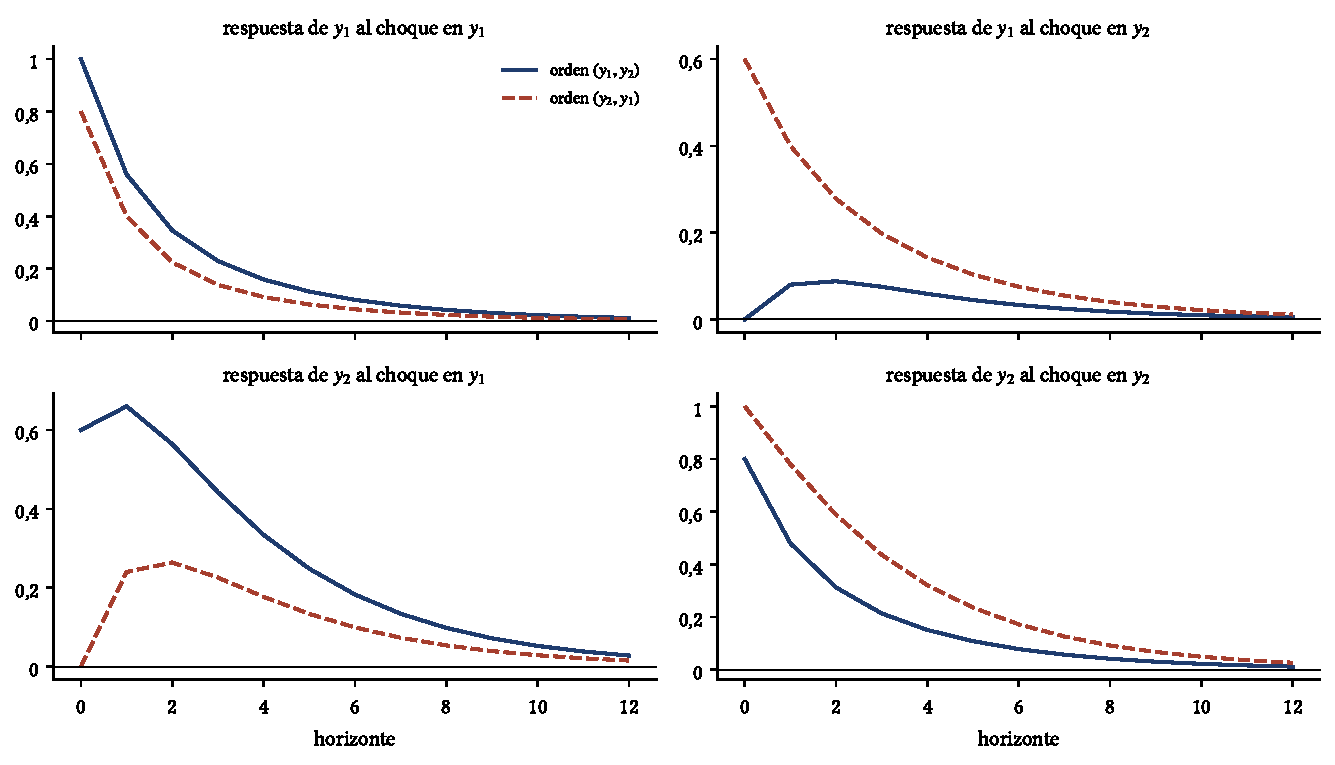
\includegraphics[width=0.92\linewidth]{graficos/cap10_fig_orden.pdf}
\caption{Respuestas ortogonalizadas de un VAR(1) bivariado con innovaciones correlacionadas ($\rho=0{,}6$) según el
orden de Cholesky. La variable ordenada primero recibe toda la correlación contemporánea.}
\label{fig:varorden}
\end{figure}

\paragraph{Alternativas.} Cuando no hay un orden natural, se pueden reportar los dos órdenes, usar las
respuestas \emph{generalizadas} de Pesaran y Shin (1998), que no dependen del orden, o imponer restricciones
basadas en la teoría económica (VAR estructurales). Las bandas de confianza se obtienen por \emph{bootstrap}:
se remuestrean los residuos, se reconstruye la serie con los coeficientes estimados, se reestima el VAR y se
recalculan las respuestas; los percentiles 5 y 95 de las réplicas forman una banda al 90\,\%.

% ---------------------------------------------------------------------
\section{Descomposición de la varianza del error de pronóstico}
% ---------------------------------------------------------------------

\begin{proposicion}[Descomposición de la varianza]\label{prop:fevd}
El error de pronóstico a $h$ períodos de $y_k$ tiene varianza
\[
  \mathrm{ECM}_k(h)=\sum_{i=0}^{h-1}\sum_{j=1}^{K}\theta_{kj,i}^2,
\]
y la proporción debida al choque $j$ es
\[
  \omega_{kj}(h)=\frac{\sum_{i=0}^{h-1}\theta_{kj,i}^2}{\mathrm{ECM}_k(h)},\qquad \sum_{j=1}^{K}\omega_{kj}(h)=1 .
\]
\end{proposicion}

\begin{proof}
El pronóstico óptimo en $T$ es la esperanza condicional. Los choques futuros, de
$\boldsymbol\varepsilon_{T+1}$ a $\boldsymbol\varepsilon_{T+h}$, son impredecibles, y los pasados son conocidos.
El error es entonces la parte de la representación de la Proposición~\ref{prop:chol} que depende de los choques
futuros:
\begin{align*}
  \mathbf y_{T+h}-\E_T[\mathbf y_{T+h}] &= \sum_{i=0}^{h-1}\Theta_i\,\boldsymbol\varepsilon_{T+h-i}.
\end{align*}
Su componente $k$ es
\begin{align*}
  y_{k,T+h}-\E_T[y_{k,T+h}] &= \sum_{i=0}^{h-1}\sum_{j=1}^{K}\theta_{kj,i}\,\varepsilon_{j,T+h-i}.
\end{align*}
Los $\varepsilon_{j,s}$ tienen varianza uno y no están correlacionados entre sí ni en el tiempo, así que la
varianza de la suma es la suma de los cuadrados de los coeficientes:
\begin{align*}
  \mathrm{ECM}_k(h) &= \sum_{i=0}^{h-1}\sum_{j=1}^{K}\theta_{kj,i}^2\,\Var(\varepsilon_{j,T+h-i})\\
                    &= \sum_{j=1}^{K}\Bigl(\sum_{i=0}^{h-1}\theta_{kj,i}^2\Bigr).
\end{align*}
Cada término entre paréntesis es la contribución del choque $j$; dividirla entre el total da $\omega_{kj}(h)$,
y las proporciones suman uno por construcción.
\end{proof}

La descomposición responde a la pregunta: ¿qué fracción de la incertidumbre sobre $y_k$ a $h$ períodos viene de
cada fuente de choques? Hereda del factor de Cholesky la dependencia del orden.

% ---------------------------------------------------------------------
\section{Ejercicios resueltos}
% ---------------------------------------------------------------------

\begin{ejresuelto}{VAR para el S\&P 500 y el VIX}\label{ej:varvix}
\enunciado Con el rendimiento logarítmico diario del S\&P 500, $r_t$, y el cambio logarítmico diario del VIX,
$\Delta v_t$, ambos en porcentaje (1999--2018), elija el orden de un VAR con AIC, BIC y HQ ($p_{\max}=10$),
estime el VAR elegido por el BIC, calcule la correlación de los residuos y verifique la estabilidad.

\solucion
\paso{Paso 1. Selección del orden.} Los tres criterios no coinciden: el AIC elige $p=10$ (el máximo), el HQ
$p=7$ y el BIC $p=2$. Con 5\,029 observaciones, el BIC penaliza cada parámetro con $\ln n/n=0{,}0017$, casi
cuatro veces más que el AIC ($2/n=0{,}0004$). Seguimos al BIC; el Ejercicio~\ref{ej:granger} verifica que las
conclusiones no cambian con $p=7$.

\paso{Paso 2. Estimación.}
\begin{center}\small
\begin{tabular}{@{}lrrrr@{}}
\toprule
 & \multicolumn{2}{c}{Ecuación de $r_t$} & \multicolumn{2}{c}{Ecuación de $\Delta v_t$} \\
\cmidrule(lr){2-3}\cmidrule(lr){4-5}
Regresor & Coeficiente & $t$ & Coeficiente & $t$ \\
\midrule
constante        & 0,0159 & 0,94 & $-0{,}0035$ & $-0{,}04$ \\
$r_{t-1}$        & $-0{,}0976$ & $-4{,}69$ & 0,1855 & 1,58 \\
$\Delta v_{t-1}$ & $-0{,}0055$ & $-1{,}50$ & $-0{,}0621$ & $-2{,}99$ \\
$r_{t-2}$        & $-0{,}0718$ & $-3{,}45$ & 0,2112 & 1,79 \\
$\Delta v_{t-2}$ & $-0{,}0049$ & $-1{,}33$ & $-0{,}0372$ & $-1{,}79$ \\
\bottomrule
\end{tabular}
\end{center}
Los rezagos propios son significativos y negativos en las dos ecuaciones: hay una leve reversión diaria. Los
rezagos cruzados no lo son con los errores clásicos.

\paso{Paso 3. Covarianza de los residuos.}
\begin{align*}
  \hat\Sigma &= \begin{bmatrix} 1{,}4376 & -5{,}9884\\ -5{,}9884 & 46{,}0708\end{bmatrix},\\[4pt]
  \hat\rho_{u}  &= \frac{-5{,}9884}{\sqrt{1{,}4376\times46{,}0708}}\\
               &= \frac{-5{,}9884}{8{,}1383}\\
               &= -0{,}7358 .
\end{align*}
La relación entre el S\&P 500 y el VIX es sobre todo \emph{contemporánea}: los días en que el índice cae, el VIX
sube mucho (Figura~\ref{fig:varvixdisp}). Una regresión simple de $\Delta v_t$ sobre $r_t$ tiene pendiente
$-4{,}17$: una caída de 1\,\% en el índice coincide con un aumento promedio de 4,2\,\% en el VIX.

\paso{Paso 4. Estabilidad.} Los módulos de los cuatro autovalores de la matriz compañera ($4\times4$) son
$0{,}2508$ (dos veces) y $0{,}2428$ (dos veces), muy por debajo de uno: el VAR es estable y los efectos de los
choques se disipan en pocos días.

\codigoweb{cap10_ej01}
\salidaR{cap10_ej01_R.txt}
\lectura{cap10_ej01}

\RvsPy Las funciones propias construyen la matriz de rezagos y resuelven $(X'X)\hat B=X'Y$ en los dos lenguajes.
En Python las comprobamos con \texttt{VAR} de \texttt{statsmodels}, que coincide en coeficientes, en
$\hat\Sigma$ y en los criterios de información, porque también usa una muestra común para seleccionar el
orden. En R, \texttt{merge} une el S\&P 500 y el VIX por fecha, igual que \texttt{pd.merge} en Python.

\begin{figure}[ht]
\centering
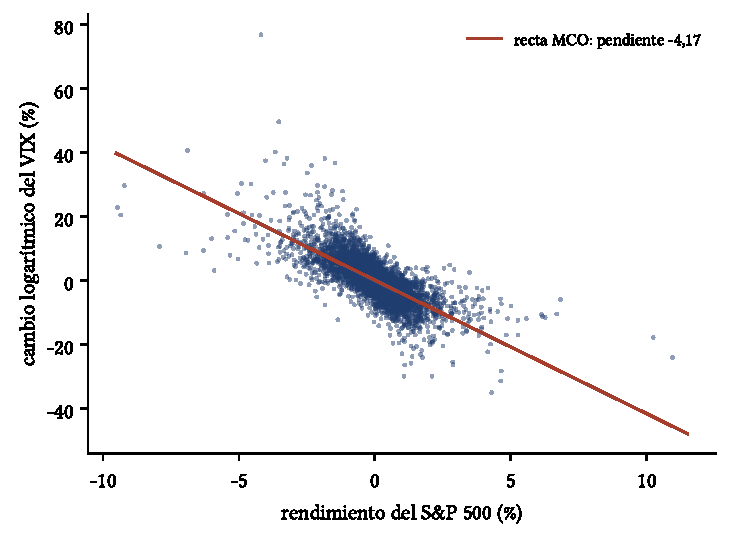
\includegraphics[width=0.62\linewidth]{graficos/cap10_ej01_dispersion.pdf}
\caption{Rendimiento diario del S\&P 500 frente al cambio logarítmico del VIX del mismo día (1999--2018).}
\label{fig:varvixdisp}
\end{figure}

\begin{conclusion}
El VAR(2) es estable. Casi toda la interacción entre el S\&P 500 y el VIX ocurre dentro del mismo día; la
dinámica rezagada es débil. Eso anticipa que el orden de Cholesky será decisivo para las respuestas al impulso.
\end{conclusion}
\end{ejresuelto}

\begin{ejresuelto}{Causalidad de Granger en dos pares de mercados}\label{ej:granger}
\enunciado Contraste la causalidad de Granger en ambas direcciones: (a) entre $r_t$ y $\Delta v_t$ con VAR(2) y
VAR(7); (b) entre las carteras mensuales S1V3 (pequeña) y S5V3 (grande) de French, con el orden elegido por BIC
y por AIC. Use la prueba $F$ y la de Wald robusta.

\solucion
\paso{Paso 1. S\&P 500 y VIX.}
\begin{center}\small
\begin{tabular}{@{}llrrrr@{}}
\toprule
Hipótesis nula & $p$ & $F$ & valor $p$ & Wald HC0 & valor $p$ \\
\midrule
$\Delta v$ no causa a $r$ & 2 & 1,870 & 0,154 & 1,947 & 0,378 \\
$r$ no causa a $\Delta v$ & 2 & 2,666 & 0,070 & 3,899 & 0,142 \\
$\Delta v$ no causa a $r$ & 7 & 1,496 & 0,164 & 6,296 & 0,506 \\
$r$ no causa a $\Delta v$ & 7 & 1,571 & 0,139 & 8,243 & 0,312 \\
\bottomrule
\end{tabular}
\end{center}
Ninguna hipótesis se rechaza al 5\,\%. El rendimiento de ayer ayuda marginalmente a predecir el cambio del VIX
con la prueba $F$ ($p=0{,}070$), pero la evidencia desaparece con la prueba robusta ($p=0{,}142$): la prueba
clásica sobrestima la significancia porque los residuos son muy heterocedásticos.

\paso{Paso 2. Carteras pequeña y grande.} El BIC elige $p=1$ y el AIC $p=5$.
\begin{center}\small
\begin{tabular}{@{}llrrrr@{}}
\toprule
Hipótesis nula & $p$ & $F$ & valor $p$ & Wald HC0 & valor $p$ \\
\midrule
grande no causa a pequeña & 1 & 3,702 & 0,055 & 2,472 & 0,116 \\
pequeña no causa a grande & 1 & 0,333 & 0,564 & 0,276 & 0,600 \\
grande no causa a pequeña & 5 & 2,083 & 0,066 & 5,615 & 0,346 \\
pequeña no causa a grande & 5 & 0,863 & 0,505 & 4,356 & 0,499 \\
\bottomrule
\end{tabular}
\end{center}
La asimetría que encontramos en el Capítulo~\ref{cap:eficiencia} reaparece (el valor $p$ en el sentido
grande$\to$pequeña es mucho menor que en el sentido contrario), pero no alcanza el 5\,\% y se debilita con la
prueba robusta. Para $p=1$, la prueba $F$ con una restricción es el cuadrado del estadístico $t$ de la
regresión del Ejercicio~\ref{ej:adelanto}: $1{,}924^2=3{,}702$.

\codigoweb{cap10_ej02}
\salidaR{cap10_ej02_R.txt}
\lectura{cap10_ej02}

\RvsPy Nuestra prueba $F$ usa una sola ecuación, con $n-q=815$ grados de libertad en el denominador.
\texttt{test\_causality} de \texttt{statsmodels} usa el sistema completo y $K(n-q)=1\,630$ grados de libertad;
el estadístico es el mismo ($3{,}702$) y el valor $p$ cambia en la cuarta decimal ($0{,}0545$ frente a
$0{,}0547$). La prueba robusta no está en \texttt{statsmodels} para el VAR, así que la programamos con la matriz
de White en los dos lenguajes.

\begin{conclusion}
En estos datos no hay causalidad de Granger significativa. Es lo esperable en mercados líquidos: si el pasado de
un precio predijera claramente a otro, los inversionistas lo aprovecharían. Además, la heterocedasticidad
puede hacer parecer significativas relaciones que no lo son, por lo que conviene reportar siempre la versión
robusta.
\end{conclusion}
\end{ejresuelto}

\begin{ejresuelto}{Respuestas al impulso entre el S\&P 500 y el VIX}\label{ej:irfvix}
\enunciado Con el VAR(2) del Ejercicio~\ref{ej:varvix}, calcule las respuestas ortogonalizadas con el orden
$(r,\Delta v)$ y con el orden $(\Delta v,r)$, y bandas \emph{bootstrap} al 90\,\% con 500 réplicas para el
primero. Calcule la respuesta acumulada del VIX a un choque positivo en el S\&P 500.

\solucion
\paso{Paso 1. Factor de Cholesky.} Con el orden $(r,\Delta v)$:
\begin{align*}
  p_{11} &= \sqrt{1{,}4376}=1{,}1990,\\
  p_{21} &= \frac{-5{,}9884}{1{,}1990}=-4{,}9945,\\
  p_{22} &= \sqrt{46{,}0708-(-4{,}9945)^2}\\
         &= \sqrt{46{,}0708-24{,}9450}\\
         &= \sqrt{21{,}1258}=4{,}5963 .
\end{align*}
Un choque de una desviación estándar en el S\&P 500 ($+1{,}20$\,\%) baja el VIX $4{,}99$\,\% el mismo día.

\paso{Paso 2. Dinámica.}
\begin{center}\small
\begin{tabular}{@{}rrrrr@{}}
\toprule
$h$ & $r\leftarrow r$ & $\Delta v\leftarrow r$ & $r\leftarrow\Delta v$ & $\Delta v\leftarrow\Delta v$ \\
\midrule
0  & 1,1990 & $-4{,}9945$ & 0,0000 & 4,5963 \\
1  & $-0{,}0895$ & 0,5328 & $-0{,}0253$ & $-0{,}2856$ \\
2  & $-0{,}0558$ & 0,3894 & $-0{,}0185$ & $-0{,}1581$ \\
5  & $-0{,}0002$ & 0,0058 & $-0{,}0006$ & 0,0009 \\
\bottomrule
\end{tabular}
\end{center}
Tras la caída inicial, el VIX rebota: sube $0{,}53$\,\% el día siguiente y $0{,}39$\,\% el segundo, y las bandas
excluyen el cero (por ejemplo, $[0{,}367;\ 0{,}696]$ en $h=1$ en R). La respuesta acumulada a 10 días es
$-4{,}16$\,\%: el VIX devuelve en dos días una sexta parte de su caída. La respuesta del S\&P 500 a un choque en
el VIX es pequeña y su banda incluye el cero o lo roza.

\paso{Paso 3. El orden importa.} Con el orden $(\Delta v,r)$, la correlación contemporánea se atribuye al VIX:
un choque en el VIX baja el S\&P 500 $0{,}88$\,\% en el impacto, y el choque ``propio'' del S\&P 500 ya no mueve
al VIX en ese período. Las respuestas en $h\ge1$ también cambian (Figura~\ref{fig:irfvix}). Con una correlación de
$-0{,}74$ entre innovaciones, el orden decide casi toda la historia: los datos no distinguen si es el mercado el
que mueve al VIX o al revés.

\codigoweb{cap10_ej03}
\salidaR{cap10_ej03_R.txt}
\lectura{cap10_ej03}

\RvsPy En R, \texttt{chol()} devuelve la triangular \emph{superior} $R$ con $R'R=\Sigma$, por lo que usamos
$P=R'$; \texttt{np.linalg.cholesky} devuelve directamente la inferior. Las respuestas puntuales coinciden con
\texttt{orth\_ma\_rep} de \texttt{statsmodels}. Las bandas \emph{bootstrap} difieren entre lenguajes en la
segunda o tercera cifra porque los generadores de números aleatorios no son los mismos, aunque usen la misma
semilla. Por ejemplo, la banda de $r\leftarrow\Delta v$ en $h=1$ es $[-0{,}0538;\ 0{,}0023]$ en R y
$[-0{,}0513;\ -0{,}0005]$ en Python: un resultado que está en el límite de la significancia puede cambiar de lado
según la simulación, lo que es en sí mismo una advertencia.

\begin{figure}[ht]
\centering
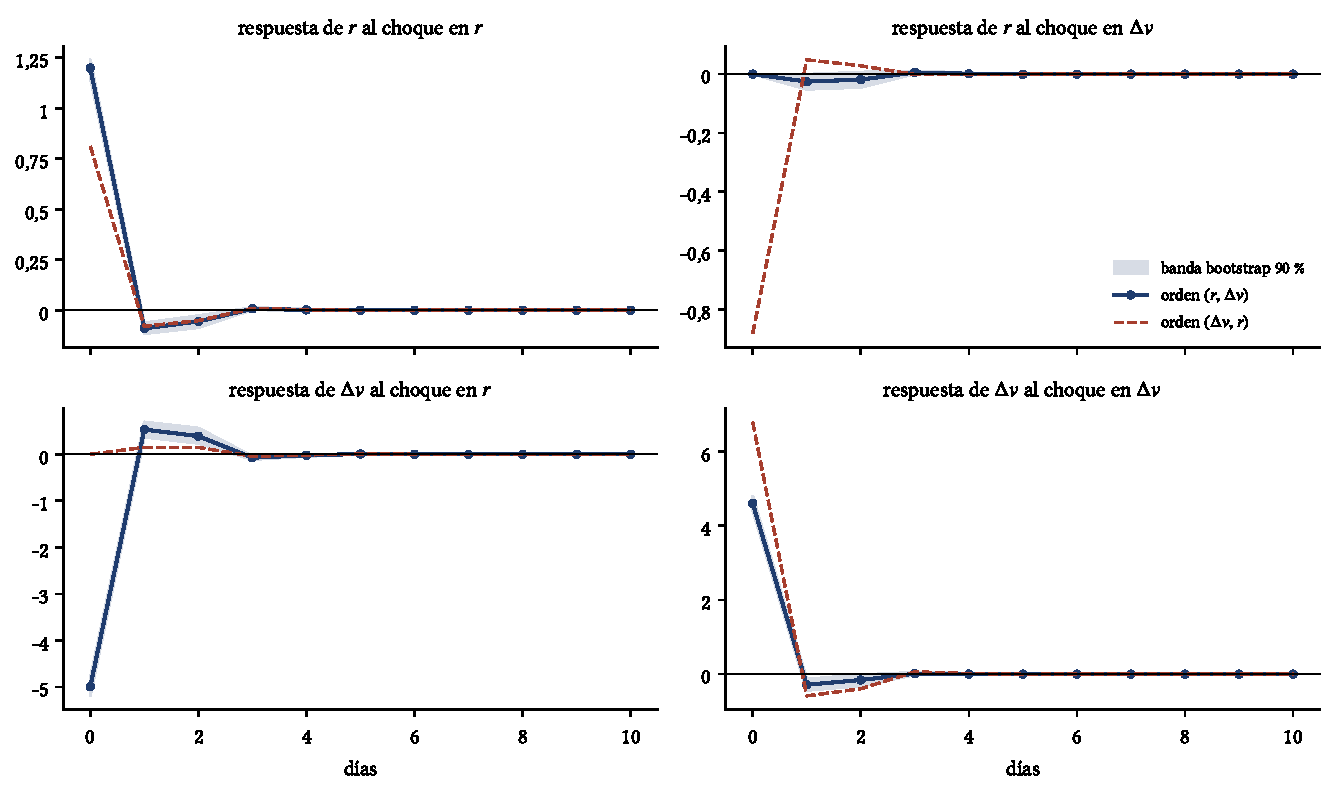
\includegraphics[width=\linewidth]{graficos/cap10_ej03_irf.pdf}
\caption{Respuestas ortogonalizadas del VAR(2) para el S\&P 500 ($r$) y el VIX ($\Delta v$), con la banda
\emph{bootstrap} al 90\,\% para el orden $(r,\Delta v)$ y la respuesta puntual con el orden inverso.}
\label{fig:irfvix}
\end{figure}

\begin{conclusion}
Un choque positivo al S\&P 500 reduce el VIX de inmediato, y el VIX corrige parcialmente en los dos días
siguientes. Como la relación es casi toda contemporánea, las respuestas dependen de forma crítica del orden de
Cholesky; conviene reportar ambos órdenes cuando la teoría no da uno.
\end{conclusion}
\end{ejresuelto}

\begin{ejresuelto}{Inflación, tasas de interés y acciones en EE.\,UU.}\label{ej:varmacro}
\enunciado Con datos mensuales de EE.\,UU.\ (1960--2023) estime un VAR con la inflación ($\mathit{inf}$, cambio
logarítmico del IPC en porcentaje), el cambio en la tasa de los bonos a 10 años ($\mathit{dtasa}$, en puntos
porcentuales) y el rendimiento total del S\&P 500 ($\mathit{ret}$, en porcentaje). Elija el orden, contraste la
causalidad de Granger y calcule respuestas y descomposición de la varianza con el orden
$(\mathit{inf},\mathit{dtasa},\mathit{ret})$.

\solucion
\paso{Paso 1. Orden.} Con $T=761$ meses y $p_{\max}=12$, el AIC elige 12, el BIC 1 y el HQ 2. Usamos $p=2$,
un compromiso que conserva algo de dinámica sin sobreajustar. El orden de Cholesky refleja que el IPC y las tasas
de largo plazo se mueven más despacio que las acciones: suponemos que las acciones pueden reaccionar en el mes
a la inflación y a las tasas, pero no al revés.

\paso{Paso 2. Causalidad de Granger.}
\begin{center}\small
\begin{tabular}{@{}lrrrr@{}}
\toprule
Hipótesis nula & $F$ & valor $p$ & Wald HC0 & valor $p$ \\
\midrule
$\mathit{dtasa}$ no causa a $\mathit{inf}$ & 5,144 & 0,006 & 9,103 & 0,011 \\
$\mathit{ret}$ no causa a $\mathit{inf}$ & 4,991 & 0,007 & 4,447 & 0,108 \\
$\mathit{inf}$ no causa a $\mathit{dtasa}$ & 8,435 & 0,000 & 12,062 & 0,002 \\
$\mathit{ret}$ no causa a $\mathit{dtasa}$ & 9,799 & 0,000 & 14,474 & 0,001 \\
$\mathit{inf}$ no causa a $\mathit{ret}$ & 1,347 & 0,261 & 2,704 & 0,259 \\
$\mathit{dtasa}$ no causa a $\mathit{ret}$ & 7,239 & 0,001 & 12,979 & 0,002 \\
$\mathit{inf}$ y $\mathit{dtasa}$ no causan a $\mathit{ret}$ & 4,866 & 0,001 & 15,663 & 0,004 \\
\bottomrule
\end{tabular}
\end{center}
A diferencia de los datos diarios, aquí sí hay causalidad de Granger robusta: los cambios pasados en la tasa de
interés ayudan a predecir el rendimiento de las acciones, y la inflación y las tasas se predicen mutuamente.

\paso{Paso 3. Respuestas del rendimiento.} Un choque de una desviación estándar en la tasa
($0{,}25$ puntos) reduce el rendimiento del S\&P 500 en $0{,}24$ puntos en el mes y en $0{,}52$ el mes
siguiente; uno en la inflación lo reduce $0{,}27$ puntos al mes siguiente. A 24 meses, las respuestas acumuladas
son $-0{,}85$ y $-0{,}56$ puntos (Figura~\ref{fig:varmacro}). Que la reacción sea mayor un mes después que en el
mes del choque se explica en parte porque el IPC se publica con rezago y porque los precios de la base de
Shiller son promedios mensuales.

\paso{Paso 4. Descomposición de la varianza.} En $h=1$ se usa la fila de $\mathit{ret}$ en $\Theta_0$:
\begin{align*}
  (\theta_{31,0},\ \theta_{32,0},\ \theta_{33,0}) &= (-0{,}0228;\ -0{,}2356;\ 3{,}4648),\\[4pt]
  \mathrm{ECM}_{\mathit{ret}}(1) &= 0{,}0228^2+0{,}2356^2+3{,}4648^2\\
                                &= 0{,}0005+0{,}0555+12{,}0048\\
                                &= 12{,}0609,\\[4pt]
  \omega_{\mathit{ret},\mathit{dtasa}}(1) &= \frac{0{,}0555}{12{,}0609}=0{,}0046 .
\end{align*}
Es decir, el choque de tasa explica el 0,46\,\% de la varianza del error a un mes.
A 24 meses, la inflación explica el $0{,}78$\,\% y la tasa el $2{,}78$\,\% de la varianza del error de pronóstico
del rendimiento; el $96{,}44$\,\% restante viene de sus propios choques.

\codigoweb{cap10_ej04}
\salidaR{cap10_ej04_R.txt}
\lectura{cap10_ej04}

\RvsPy La descomposición de \texttt{statsmodels} (\texttt{fevd}) coincide con la nuestra. Atención con los
índices: nuestra función guarda los horizontes $h=0,1,\dots$, de modo que la proporción a $h$ períodos está en la
posición $h-1$ en Python y en la fila $h$ en R.

\begin{figure}[ht]
\centering
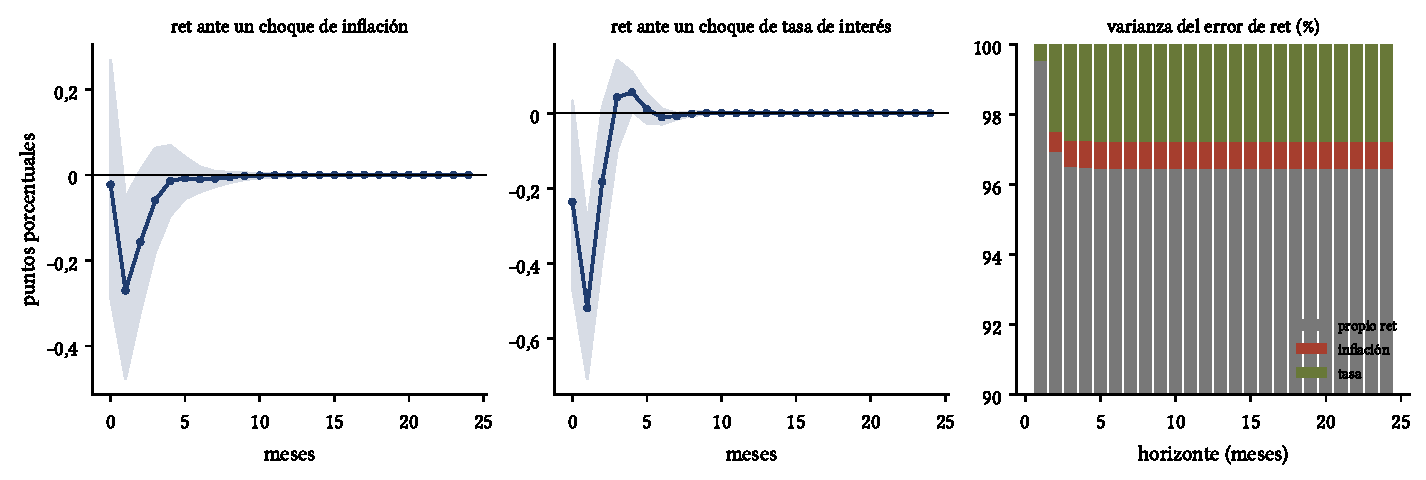
\includegraphics[width=\linewidth]{graficos/cap10_ej04_macro.pdf}
\caption{Respuesta del rendimiento del S\&P 500 a choques de inflación y de tasa de interés (con banda
\emph{bootstrap} al 90\,\%) y descomposición de la varianza de su error de pronóstico; el eje vertical del panel
derecho empieza en 90\,\%.}
\label{fig:varmacro}
\end{figure}

\begin{conclusion}
Las tasas de interés y la inflación predicen las acciones de forma estadísticamente robusta, con el signo que
predice la teoría (más inflación y más tasa, menor rendimiento). Pero la magnitud es pequeña: explican menos del
4\,\% de la incertidumbre sobre el rendimiento del mes siguiente.
\end{conclusion}
\end{ejresuelto}

\begin{ejresuelto}{¿Pronostica el VAR mejor que la media histórica?}\label{ej:varfuera}
\enunciado Para el rendimiento mensual de la cartera pequeña S1V3, genere pronósticos a un mes desde enero de
1983 con ventana creciente usando: (i) la media histórica, (ii) un AR(1) y (iii) la ecuación de la cartera
pequeña de un VAR(1) con la grande. Calcule el $R^2$ fuera de muestra y aplique la prueba de Clark y West.

\solucion
\paso{Paso 1. El $R^2$ fuera de muestra.} Campbell y Thompson (2008) lo definen respecto de la media histórica:
\[
  R^2_{\text{FM}}=1-\frac{\sum_t(y_t-\hat y_t^{\text{modelo}})^2}{\sum_t(y_t-\bar y_t)^2},
\]
donde $\bar y_t$ es la media con datos hasta $t-1$. Es positivo si el modelo pronostica mejor que la media. Con
411 meses de evaluación (enero de 1983 a marzo de 2017), los errores cuadráticos medios son 30,72 (media), 30,09
(AR) y 30,00 (VAR):
\begin{align*}
  R^2_{\text{FM}}(\text{AR}) &= 1-\frac{30{,}0903}{30{,}7166}=0{,}0204,\\
  R^2_{\text{FM}}(\text{VAR}) &= 1-\frac{29{,}9954}{30{,}7166}=0{,}0235,
\end{align*}
es decir, 2,04\,\% y 2,35\,\%.

\paso{Paso 2. Prueba de Clark y West.} Cuando un modelo está anidado en otro, la prueba de Diebold-Mariano está
sesgada contra el modelo grande, que debe estimar parámetros que bajo la nula valen cero. Clark y West (2007)
corrigen ese sesgo con
\[
  f_t=e_{1t}^2-\bigl[e_{2t}^2-(\hat y_{1t}-\hat y_{2t})^2\bigr],
\]
y contrastan unilateralmente que $\E[f_t]=0$ con un estadístico $t$ de Newey-West. Resultados: media frente a
AR(1), $t=2{,}73$ ($p=0{,}003$); media frente a VAR(1), $t=2{,}79$ ($p=0{,}003$); AR(1) frente a VAR(1), $t=1{,}17$
($p=0{,}121$). Los rendimientos pasados de la cartera pequeña ayudan a pronosticarla fuera de muestra; agregar la
cartera grande no mejora significativamente.

\paso{Paso 3. Estabilidad en el tiempo.} El $R^2_{\text{FM}}$ es de $5{,}69$\,\% (AR) y $5{,}09$\,\% (VAR) en
1983--1999, pero de $-0{,}58$\,\% y $0{,}38$\,\% en 2000--2017. La Figura~\ref{fig:varfuera} muestra que la ventaja se
acumula hasta 2000 y luego se estanca: la predictibilidad de las acciones pequeñas casi desapareció en las
últimas dos décadas.

\codigoweb{cap10_ej05}
\salidaR{cap10_ej05_R.txt}
\lectura{cap10_ej05}

\RvsPy El bucle de ventana creciente es idéntico: en R reestimamos con \texttt{lm} y en Python con
\texttt{np.linalg.lstsq}. Cuidado con los índices: en R el primer mes pronosticado es la fila
\texttt{which(f\$dates == "1983-01")}; en Python, que cuenta desde cero, \texttt{np.flatnonzero(...)[0]}, y en
ambos casos la estimación usa solo datos anteriores.

\begin{figure}[ht]
\centering
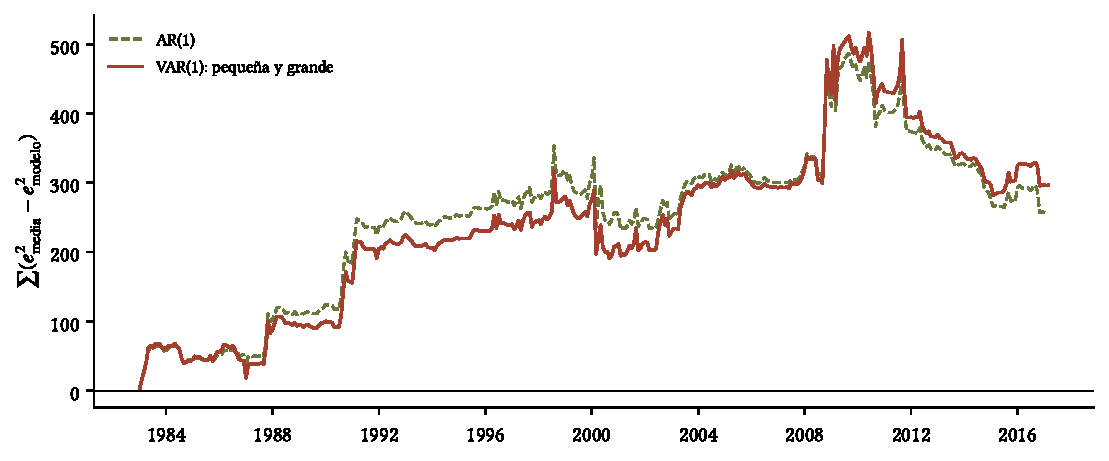
\includegraphics[width=0.88\linewidth]{graficos/cap10_ej05_fuera_muestra.pdf}
\caption{Diferencia acumulada entre los errores cuadráticos de la media histórica y los del modelo. Una curva
que sube indica que el modelo pronostica mejor; después de 2000 la curva deja de subir.}
\label{fig:varfuera}
\end{figure}

\begin{conclusion}
Un modelo dinámico sencillo pronostica la cartera pequeña algo mejor que la media histórica, con significancia
estadística. Pero la ganancia se concentra antes de 2000, y la información de la cartera grande no aporta casi
nada adicional. En pronóstico financiero, los modelos parsimoniosos suelen ser tan buenos como los complejos.
\end{conclusion}
\end{ejresuelto}

% ---------------------------------------------------------------------
\section{Ejercicios propuestos}
% ---------------------------------------------------------------------

\begin{enumerate}[label=\textbf{\thechapter.\arabic*},leftmargin=*,itemsep=6pt]
  \item Escriba la matriz compañera de un VAR(2) bivariado y demuestre que, si $A_2=0$, sus autovalores son los
  de $A_1$ más dos ceros.

  \item Para el VAR(1) con $A_1=\bigl[\begin{smallmatrix}0{,}5&0{,}1\\0{,}3&0{,}6\end{smallmatrix}\bigr]$, calcule
  los autovalores y $\Psi_2$. \textit{Respuesta: $0{,}7303$ y $0{,}3697$;
  $\Psi_2=\bigl[\begin{smallmatrix}0{,}28&0{,}11\\0{,}33&0{,}39\end{smallmatrix}\bigr]$.}

  \item Con $\Sigma=\bigl[\begin{smallmatrix}4&1\\1&2\end{smallmatrix}\bigr]$, calcule el factor de Cholesky
  con el orden $(y_1,y_2)$ y con el orden $(y_2,y_1)$. \textit{Respuesta:
  $\bigl[\begin{smallmatrix}2&0\\0{,}5&1{,}3229\end{smallmatrix}\bigr]$; con el orden inverso, $y_2$ recibe
  $\sqrt2=1{,}4142$ en su propio choque e $y_1$ recibe $0{,}7071$ y $1{,}8708$.}

  \item Demuestre que, en un VAR bivariado, si $y_2$ no causa a $y_1$ en el sentido de Granger, entonces
  $\Psi_i[1,2]=0$ para todo $i$.

  \item Demuestre que la descomposición de la varianza a un período con el orden $(y_1,y_2)$ atribuye el
  100\,\% de la varianza de $y_1$ a su propio choque.

  \item \emph{(Simulación.)} Simule 1\,000 muestras de $T=200$ observaciones de dos paseos aleatorios
  independientes y estime un VAR(1) en niveles. ¿Con qué frecuencia rechaza la prueba $F$ al 5\,\% la hipótesis
  de no causalidad? Compare con un VAR en primeras diferencias.

  \item \emph{(Con datos del BCRP.)} Estime un VAR mensual con la inflación, el tipo de cambio sol/dólar y la
  tasa de referencia del BCRP. Elija un orden de Cholesky justificado y calcule la respuesta de la inflación a
  un choque cambiario (traspaso del tipo de cambio).

  \item \emph{(Con datos.)} Repita el Ejercicio~\ref{ej:irfvix} con un VAR de tres variables que agregue el
  rendimiento diario del Brent. ¿Qué fracción de la varianza del error de pronóstico del S\&P 500 explican los
  choques del petróleo?
\end{enumerate}

% ---------------------------------------------------------------------
\section{Resumen de fórmulas}
% ---------------------------------------------------------------------

\begin{table}[H]
\centering\small
\begin{tabular}{@{}ll@{}}
\toprule
Concepto & Fórmula \\
\midrule
VAR($p$) & $\mathbf y_t=\mathbf c+\sum_{j=1}^{p}A_j\mathbf y_{t-j}+\mathbf u_t$,\quad $\E[\mathbf u_t\mathbf u_t']=\Sigma$ \\
Estabilidad & autovalores de la matriz compañera $F$ con $|\lambda|<1$ \\
Medias móviles & $\Psi_0=I$,\quad $\Psi_i=\sum_{j=1}^{\min(i,p)}A_j\Psi_{i-j}$ \\
Estimador & $\hat B=(X'X)^{-1}X'Y$ (MCO por ecuación $=$ MCG) \\
Criterios & $\ln|\tilde\Sigma_p|+c_n\,(pK^2+K)/n$;\quad $c_n=2,\ \ln n,\ 2\ln\ln n$ \\
Granger & $F=[(\mathrm{SRC}_r-\mathrm{SRC}_u)/r]/[\mathrm{SRC}_u/(n-q)]$ \\
Cholesky & $PP'=\Sigma$,\quad $\Theta_i=\Psi_iP$ \\
Descomposición & $\omega_{kj}(h)=\sum_{i<h}\theta_{kj,i}^2\big/\sum_{i<h}\sum_m\theta_{km,i}^2$ \\
$R^2$ fuera de muestra & $1-\sum(y_t-\hat y_t)^2/\sum(y_t-\bar y_t)^2$ \\
\bottomrule
\end{tabular}
\caption{Fórmulas principales del Capítulo 10.}
\end{table}

\section*{Referencias}
\begin{itemize}[leftmargin=*]
  \item Campbell, J. Y. y Thompson, S. B. (2008). Predicting excess stock returns out of sample: Can anything beat
        the historical average? \emph{Review of Financial Studies}, 21(4), 1509--1531.
  \item Clark, T. E. y West, K. D. (2007). Approximately normal tests for equal predictive accuracy in nested
        models. \emph{Journal of Econometrics}, 138(1), 291--311.
  \item Granger, C. W. J. (1969). Investigating causal relations by econometric models and cross-spectral
        methods. \emph{Econometrica}, 37(3), 424--438.
  \item Kilian, L. y Lütkepohl, H. (2017). \emph{Structural Vector Autoregressive Analysis}. Cambridge University
        Press.
  \item Lütkepohl, H. (2005). \emph{New Introduction to Multiple Time Series Analysis}. Springer.
  \item Pesaran, H. H. y Shin, Y. (1998). Generalized impulse response analysis in linear multivariate models.
        \emph{Economics Letters}, 58(1), 17--29.
  \item Sims, C. A. (1980). Macroeconomics and reality. \emph{Econometrica}, 48(1), 1--48.
\end{itemize}

% =====================================================================
%  Capítulo 11. Cointegración y modelos de corrección de errores
% =====================================================================
\chapter[Cointegración y VECM]{Cointegración y modelos vectoriales de corrección de errores}\label{cap:cointegracion}

\section*{Objetivos de aprendizaje}
Al terminar este capítulo, el lector podrá:
\begin{enumerate}[label=\arabic*.,leftmargin=*]
  \item Definir la cointegración y distinguirla de la regresión espuria.
  \item Reescribir un VAR en niveles como un modelo vectorial de corrección de errores (VECM) e interpretar sus
        matrices $\alpha$ y $\beta$.
  \item Aplicar la prueba de dos etapas de Engle y Granger y las pruebas de la traza y del máximo autovalor de
        Johansen, y contrastar restricciones sobre el vector de cointegración.
  \item Reconocer los cambios de régimen en una relación de largo plazo y evaluar si la corrección de errores
        mejora los pronósticos.
\end{enumerate}

\section*{Motivación}
El Capítulo~\ref{cap:raiz} mostró que los precios suelen tener raíz unitaria y que regresar un paseo aleatorio
sobre otro independiente produce relaciones espurias. Pero hay precios que \emph{no} son independientes: el
petróleo Brent y el WTI son casi el mismo producto, y si uno se encarece mucho respecto del otro, los
comerciantes compran el barato y venden el caro hasta cerrar la brecha. Cada precio deambula sin rumbo fijo,
pero la diferencia entre ellos se mantiene acotada. Esa idea, la \emph{cointegración} (Engle y Granger, 1987),
describe muchas relaciones financieras: el precio al contado y el de futuros, las tasas de interés de distintos
plazos, los precios de un mismo activo en dos mercados y, según la teoría, el precio de una acción y sus
dividendos.

\paragraph{Datos del capítulo.} Promedios mensuales de los precios diarios del Brent y del WTI de la EIA de
EE.\,UU.\ (mayo de 1987 a octubre de 2026, $T=474$) y datos anuales de precios, dividendos y utilidades reales del
S\&P 500 de la base de Shiller (1871--2023). Usamos promedios mensuales porque el 20 de abril de 2020 el WTI
cerró en $-36{,}98$ dólares, un precio negativo cuyo logaritmo no existe; los promedios mensuales son siempre
positivos.

% ---------------------------------------------------------------------
\section{Cointegración}
% ---------------------------------------------------------------------

\begin{definicion}[Cointegración; Engle y Granger, 1987]
Las componentes del vector $\mathbf y_t$ ($K\times1$) están \emph{cointegradas} si cada una es I(1) y existe un
vector $\boldsymbol\beta\ne\mathbf 0$ tal que $\boldsymbol\beta'\mathbf y_t$ es I(0). El vector
$\boldsymbol\beta$ es un \emph{vector de cointegración}, y $\boldsymbol\beta'\mathbf y_t$ la \emph{relación de
equilibrio}. El número de vectores de cointegración linealmente independientes, $r$, es el \emph{rango de
cointegración}; $0<r<K$.
\end{definicion}

Un modelo sencillo con $K=2$ lo ilustra. Sea $w_t$ un paseo aleatorio, la tendencia común, y $z_t$ un proceso
estacionario. Si
\begin{align*}
  y_{1t} &= w_t+\tfrac12 z_t,\\
  y_{2t} &= w_t-\tfrac12 z_t,
\end{align*}
cada precio hereda la raíz unitaria de $w_t$, pero
\begin{align*}
  y_{1t}-y_{2t} &= \bigl(w_t+\tfrac12z_t\bigr)-\bigl(w_t-\tfrac12z_t\bigr)\\
                &= z_t,
\end{align*}
que es estacionario: $\boldsymbol\beta=(1,-1)'$. La Figura~\ref{fig:cointsim} contrasta este caso con dos
paseos aleatorios independientes, cuya diferencia es otro paseo aleatorio que se aleja sin volver.

\begin{figure}[ht]
\centering
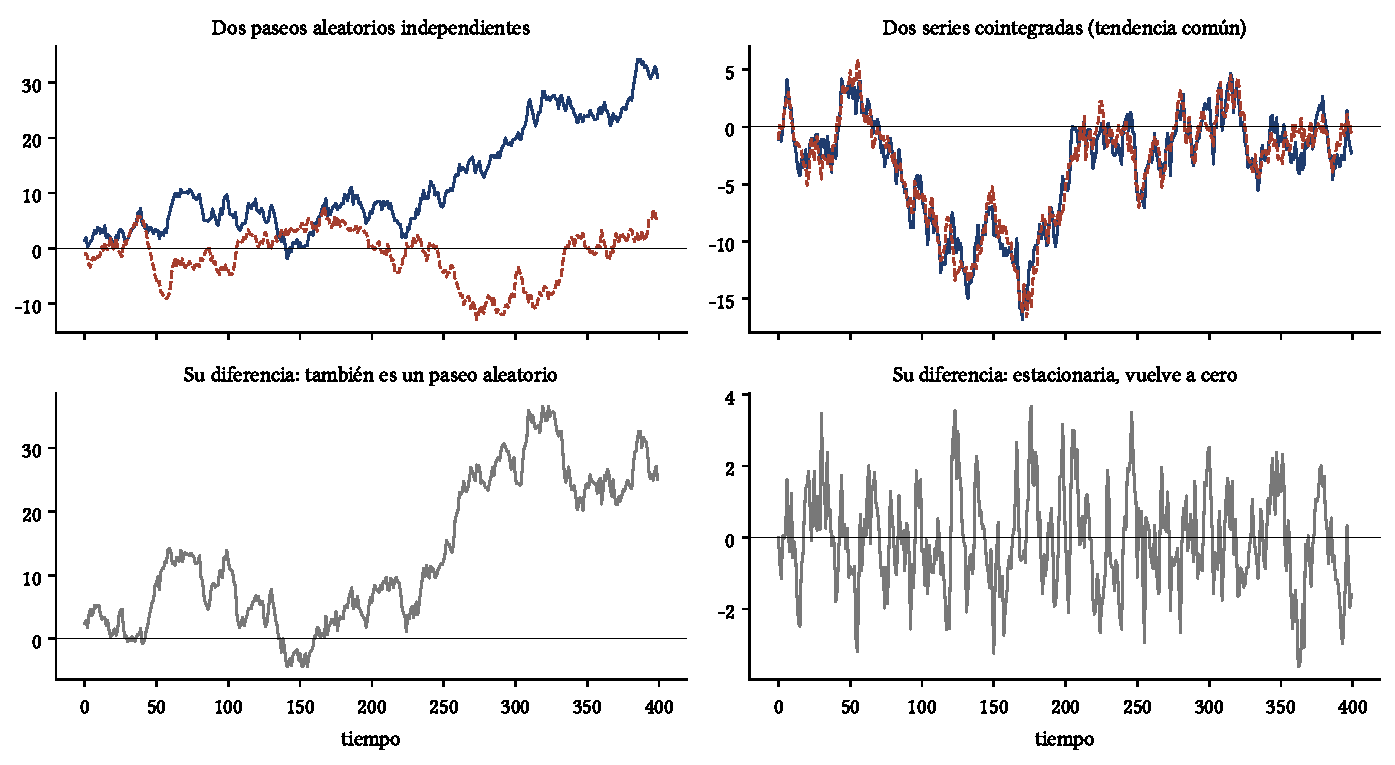
\includegraphics[width=\linewidth]{graficos/cap11_fig_coint_sim.pdf}
\caption{Izquierda: dos paseos aleatorios independientes y su diferencia, que no tiene nivel al que regresar.
Derecha: dos series cointegradas con una tendencia común y su diferencia, que fluctúa alrededor de cero.}
\label{fig:cointsim}
\end{figure}

% ---------------------------------------------------------------------
\section{El modelo vectorial de corrección de errores}
% ---------------------------------------------------------------------

\begin{proposicion}[Del VAR al VECM]\label{prop:vecm}
Todo VAR($p$) en niveles,
$\mathbf y_t=\mathbf c+A_1\mathbf y_{t-1}+\dots+A_p\mathbf y_{t-p}+\mathbf u_t$, puede escribirse como
\[
  \Delta\mathbf y_t=\mathbf c+\Pi\,\mathbf y_{t-1}+\sum_{i=1}^{p-1}\Gamma_i\,\Delta\mathbf y_{t-i}+\mathbf u_t,
\]
con $\Pi=-(I_K-A_1-\dots-A_p)$ y $\Gamma_i=-(A_{i+1}+\dots+A_p)$.
\end{proposicion}

\begin{proof}
Lo mostramos para $p=2$; el caso general sigue el mismo procedimiento. Restamos $\mathbf y_{t-1}$ a ambos lados,
y sumamos y restamos $A_2\mathbf y_{t-1}$ en el lado derecho:
\begin{align*}
  \mathbf y_t-\mathbf y_{t-1} &= \mathbf c+A_1\mathbf y_{t-1}-\mathbf y_{t-1}+A_2\mathbf y_{t-2}+\mathbf u_t\\
                              &= \mathbf c+(A_1-I_K)\mathbf y_{t-1}+A_2\mathbf y_{t-1}-A_2\mathbf y_{t-1}+A_2\mathbf y_{t-2}+\mathbf u_t\\
                              &= \mathbf c+(A_1+A_2-I_K)\mathbf y_{t-1}-A_2(\mathbf y_{t-1}-\mathbf y_{t-2})+\mathbf u_t,\\[4pt]
  \Delta\mathbf y_t           &= \mathbf c+\Pi\,\mathbf y_{t-1}+\Gamma_1\Delta\mathbf y_{t-1}+\mathbf u_t,
\end{align*}
con $\Pi=-(I_K-A_1-A_2)$ y $\Gamma_1=-A_2$.
\end{proof}

El rango de $\Pi$ determina el tipo de sistema:
\begin{itemize}[leftmargin=*]
  \item $\operatorname{rango}(\Pi)=K$: $\Pi$ es invertible, y $\mathbf y_{t-1}=\Pi^{-1}(\Delta\mathbf y_t-\dots)$ es
        estacionario porque el lado derecho lo es. Todas las variables son I(0).
  \item $\operatorname{rango}(\Pi)=0$: $\Pi=0$ y el modelo es un VAR en primeras diferencias. No hay cointegración.
  \item $0<\operatorname{rango}(\Pi)=r<K$: $\Pi$ se factoriza como $\Pi=\alpha\beta'$, con $\alpha$ y $\beta$ de
        dimensión $K\times r$. Como $\Delta\mathbf y_t$ es estacionario, también debe serlo
        $\alpha\beta'\mathbf y_{t-1}$, y por tanto $\beta'\mathbf y_{t-1}$: hay $r$ relaciones de
        cointegración.
\end{itemize}

En el tercer caso el modelo es el \emph{VECM}:
\[
  \Delta\mathbf y_t=\mathbf c+\alpha\,\bigl(\beta'\mathbf y_{t-1}\bigr)+\sum_{i=1}^{p-1}\Gamma_i\Delta\mathbf y_{t-i}+\mathbf u_t .
\]
El término $\beta'\mathbf y_{t-1}$ mide el desequilibrio del período anterior, y $\alpha$ contiene las
\emph{velocidades de ajuste}: cuánto corrige cada variable ante ese desequilibrio. Si $\beta=(1,-1)'$ y el
desequilibrio es positivo ($y_1$ caro respecto de $y_2$), la corrección exige $\alpha_1<0$ (que $y_1$ baje),
$\alpha_2>0$ (que $y_2$ suba) o ambas. Una variable con $\alpha_i=0$ es \emph{débilmente exógena}: no reacciona al
desequilibrio y es la que ``lidera'' el precio común.

\begin{proposicion}[Persistencia del desequilibrio y tendencia común]\label{prop:ajustevecm}
Sea un VECM bivariado sin rezagos ni constante,
$\Delta\mathbf y_t=\alpha\beta'\mathbf y_{t-1}+\mathbf u_t$, con $\beta=(1,-1)'$ y $\alpha=(\alpha_1,\alpha_2)'$.
Entonces:
\begin{enumerate}[label=(\roman*)]
  \item el desequilibrio $z_t=\beta'\mathbf y_t$ sigue un AR(1) con coeficiente $1+\beta'\alpha=1+\alpha_1-\alpha_2$;
  \item sin nuevos choques, ambas variables convergen a un nivel común; tras un choque inicial
        $\mathbf y_0=(1,0)'$, ese nivel es $\alpha_2/(\alpha_2-\alpha_1)$.
\end{enumerate}
\end{proposicion}

\begin{proof}
(i) Multiplicamos el modelo por $\beta'$:
\begin{align*}
  \beta'\mathbf y_t-\beta'\mathbf y_{t-1} &= \beta'\alpha\,\beta'\mathbf y_{t-1}+\beta'\mathbf u_t,\\
  z_t &= (1+\beta'\alpha)\,z_{t-1}+\beta'\mathbf u_t,\\
  1+\beta'\alpha &= 1+\alpha_1-\alpha_2 .
\end{align*}
(ii) El vector $\alpha_\perp=(\alpha_2,-\alpha_1)'$ cumple $\alpha_\perp'\alpha=\alpha_2\alpha_1-\alpha_1\alpha_2=0$.
Multiplicando el modelo sin choques por $\alpha_\perp'$:
\begin{align*}
  \alpha_\perp'\Delta\mathbf y_t &= \alpha_\perp'\alpha\,\beta'\mathbf y_{t-1}\\
                                 &= 0 .
\end{align*}
La combinación $\alpha_\perp'\mathbf y_t=\alpha_2y_{1t}-\alpha_1y_{2t}$ no cambia nunca: es la tendencia común.
Al inicio vale $\alpha_2\cdot1-\alpha_1\cdot0=\alpha_2$. Al final el desequilibrio desaparece y
$y_1=y_2=\ell$, así que
\begin{align*}
  \alpha_2\ell-\alpha_1\ell &= \alpha_2,\\
  \ell &= \frac{\alpha_2}{\alpha_2-\alpha_1}. && \qedhere
\end{align*}
\end{proof}

La Figura~\ref{fig:ajuste} muestra la proposición con $1+\beta'\alpha=0{,}75$ en los dos casos. Con
$\alpha=(-0{,}05;\,0{,}20)$ casi todo el ajuste lo hace $y_2$, y el nivel final es $0{,}20/0{,}25=0{,}8$: el choque a
$y_1$ es en su mayor parte permanente. Con $\alpha=(-0{,}20;\,0{,}05)$, el ajuste lo hace $y_1$ y el nivel final es
$0{,}05/0{,}25=0{,}2$: el choque se deshace casi por completo. La variable que no ajusta es la que fija el precio.

\begin{figure}[ht]
\centering
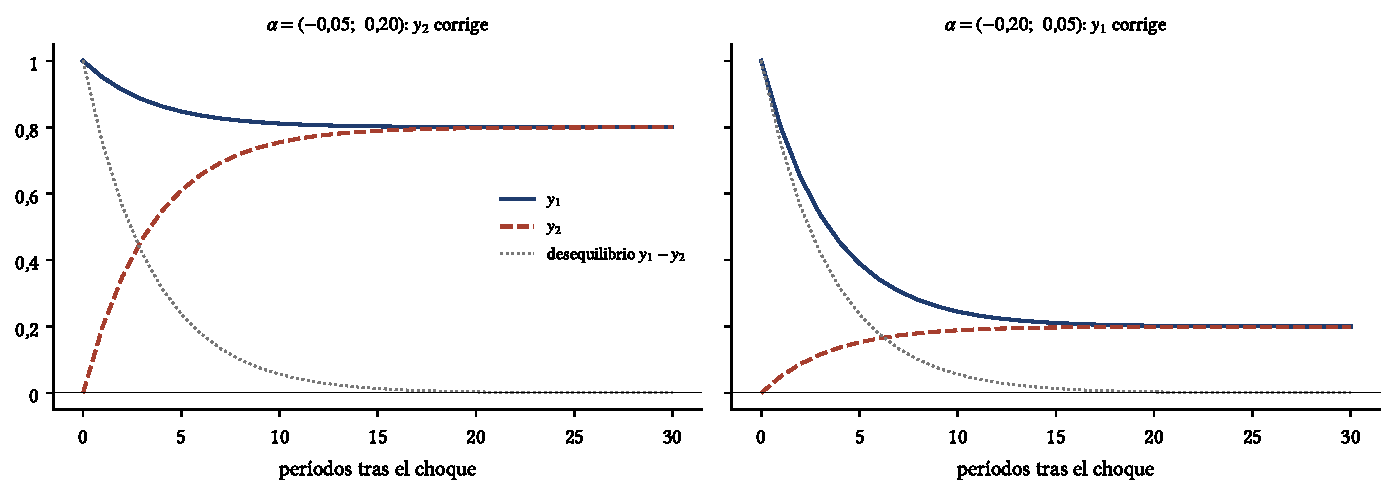
\includegraphics[width=\linewidth]{graficos/cap11_fig_ajuste.pdf}
\caption{Respuesta de un VECM bivariado con $\beta=(1,-1)'$ a un choque de $+1$ en $y_1$. Ambas variables
convergen a un nivel común; quién ajusta lo deciden los coeficientes $\alpha$.}
\label{fig:ajuste}
\end{figure}

% ---------------------------------------------------------------------
\section{El método de dos etapas de Engle y Granger}
% ---------------------------------------------------------------------

Con $K=2$ y a lo sumo una relación de cointegración, Engle y Granger (1987) proponen:
\begin{enumerate}[leftmargin=*]
  \item Estimar por MCO la regresión de cointegración $y_{1t}=a+b\,y_{2t}+u_t$.
  \item Aplicar una prueba ADF \emph{sin constante} a los residuos $\hat u_t$:
        $\Delta\hat u_t=\gamma\hat u_{t-1}+\sum_j\delta_j\Delta\hat u_{t-j}+e_t$. Si $\gamma<0$ es significativo,
        los residuos son estacionarios y las series están cointegradas.
\end{enumerate}

Hay dos sutilezas. Primero, el estimador de $b$ es \emph{superconsistente}: converge a una velocidad $T$ en
lugar de $\sqrt T$. La razón es que el regresor I(1) tiene una varianza muestral que crece con $T$: si $b$ fuera
incorrecto, los residuos serían I(1) y su suma de cuadrados crecería como $T^2$, mientras que con el $b$
correcto crece solo como $T$. Minimizar la suma de cuadrados ``encuentra'' el $b$ correcto muy rápido, aunque
$u_t$ esté correlacionado con $y_{2t}$. Segundo, los valores críticos de la prueba ADF \emph{no} son los de
Dickey y Fuller: como $\hat b$ se eligió para que los residuos parezcan lo más estacionarios posible, la prueba
rechaza con más facilidad, y hay que exigir más. MacKinnon (2010) da superficies de respuesta
$c(T)=b_\infty+b_1/T+b_2/T^2$; con dos variables y constante, el valor crítico asintótico al 5\,\% es $-3{,}34$, en
lugar de $-2{,}86$.

El método tiene limitaciones: el resultado puede depender de qué variable se pone a la izquierda, no permite
probar más de una relación y no ofrece una prueba directa sobre $b$, porque la distribución de $\hat b$ no es
estándar. El método de Johansen resuelve los tres problemas.

% ---------------------------------------------------------------------
\section{El método de Johansen}
% ---------------------------------------------------------------------

Johansen (1988, 1991) estima el VECM por máxima verosimilitud con la restricción de rango
$\Pi=\alpha\beta'$. Sean $R_{0t}$ y $R_{1t}$ los residuos de regresar, respectivamente, $\Delta\mathbf y_t$ y
$\mathbf y_{t-1}$ sobre la constante y los rezagos $\Delta\mathbf y_{t-1},\dots,\Delta\mathbf y_{t-p+1}$, y
\[
  S_{ij}=\frac1n\sum_{t}R_{it}R_{jt}',\qquad i,j\in\{0,1\}.
\]

\begin{proposicion}[Estimador y prueba de la traza de Johansen]\label{prop:johansen}
Sean $\hat\lambda_1>\dots>\hat\lambda_K$ los autovalores de $S_{11}^{-1}S_{10}S_{00}^{-1}S_{01}$ y
$\hat{\mathbf v}_i$ sus autovectores, normalizados con $\hat{\mathbf v}_i'S_{11}\hat{\mathbf v}_i=1$. Con rango $r$:
\begin{enumerate}[label=(\roman*)]
  \item $\hat\beta=(\hat{\mathbf v}_1,\dots,\hat{\mathbf v}_r)$ y $\hat\alpha=S_{01}\hat\beta$;
  \item la verosimilitud máxima cumple $L_{\max}^{-2/n}\propto|S_{00}|\prod_{i=1}^{r}(1-\hat\lambda_i)$;
  \item el estadístico de razón de verosimilitudes de $H_0$: rango $\le r$ frente a rango $=K$ es
        \[
          \lambda_{\text{traza}}(r)=-n\sum_{i=r+1}^{K}\ln\bigl(1-\hat\lambda_i\bigr).
        \]
\end{enumerate}
\end{proposicion}

\begin{proof}
Por el teorema de Frisch-Waugh-Lovell, una vez concentrados los parámetros de corto plazo, el modelo es
$R_{0t}=\alpha\beta'R_{1t}+\mathbf u_t$. Para $\beta$ fijo, es una regresión de $R_{0t}$ sobre
$\beta'R_{1t}$, con soluciones
\begin{align*}
  \hat\alpha(\beta)  &= S_{01}\beta\,(\beta'S_{11}\beta)^{-1},\\
  \hat\Sigma(\beta) &= S_{00}-S_{01}\beta\,(\beta'S_{11}\beta)^{-1}\beta'S_{10}.
\end{align*}
Con errores normales, la verosimilitud concentrada cumple $L_{\max}^{-2/n}\propto|\hat\Sigma(\beta)|$. Usamos la
identidad de determinantes de matrices por bloques,
$|A|\,|D-CA^{-1}B|=|D|\,|A-BD^{-1}C|$, con $A=S_{00}$, $B=S_{01}\beta$, $C=\beta'S_{10}$ y $D=\beta'S_{11}\beta$:
\begin{align*}
  |\hat\Sigma(\beta)| &= \bigl|S_{00}-S_{01}\beta(\beta'S_{11}\beta)^{-1}\beta'S_{10}\bigr|\\
                      &= |S_{00}|\,\frac{\bigl|\beta'S_{11}\beta-\beta'S_{10}S_{00}^{-1}S_{01}\beta\bigr|}{|\beta'S_{11}\beta|}\\
                      &= |S_{00}|\,\frac{\bigl|\beta'\bigl(S_{11}-S_{10}S_{00}^{-1}S_{01}\bigr)\beta\bigr|}{|\beta'S_{11}\beta|}.
\end{align*}
Minimizar un cociente de determinantes de este tipo es un problema de autovalores generalizados: el mínimo se
alcanza con las columnas de $\beta$ iguales a los autovectores de
$\bigl|\lambda S_{11}-S_{10}S_{00}^{-1}S_{01}\bigr|=0$ con los $r$ autovalores mayores. Con la normalización
$\beta'S_{11}\beta=I_r$, se tiene $\beta'S_{10}S_{00}^{-1}S_{01}\beta=\operatorname{diag}(\hat\lambda_1,\dots,\hat\lambda_r)$ y
\begin{align*}
  |\hat\Sigma(\hat\beta)| &= |S_{00}|\,\frac{\bigl|I_r-\operatorname{diag}(\hat\lambda_1,\dots,\hat\lambda_r)\bigr|}{|I_r|}\\
                          &= |S_{00}|\prod_{i=1}^{r}(1-\hat\lambda_i),
\end{align*}
y $\hat\alpha=S_{01}\hat\beta(\hat\beta'S_{11}\hat\beta)^{-1}=S_{01}\hat\beta$. La razón de verosimilitudes entre
el rango $r$ y el rango completo $K$ es entonces
\begin{align*}
  -2\ln\frac{L_{\max}(r)}{L_{\max}(K)} &= n\ln\frac{|S_{00}|\prod_{i=1}^{r}(1-\hat\lambda_i)}{|S_{00}|\prod_{i=1}^{K}(1-\hat\lambda_i)}\\
                                       &= -n\sum_{i=r+1}^{K}\ln(1-\hat\lambda_i). && \qedhere
\end{align*}
\end{proof}

Los autovalores son las correlaciones canónicas al cuadrado entre $\Delta\mathbf y_t$ y $\mathbf y_{t-1}$, una
vez descontada la dinámica de corto plazo: un $\hat\lambda_i$ cercano a cero indica una combinación de niveles que
no ayuda a explicar los cambios, es decir, que no es una relación de equilibrio. La prueba se aplica en
secuencia: se contrasta $r=0$; si se rechaza, $r\le1$, y así hasta no rechazar. El estadístico del \emph{máximo
autovalor}, $\lambda_{\max}(r)=-n\ln(1-\hat\lambda_{r+1})$, contrasta rango $r$ frente a $r+1$. Las distribuciones
no son estándar y dependen de los términos deterministas; usamos los valores críticos de MacKinnon, Haug y
Michelis (1999) para el caso de constante sin restringir. Con $K-r=1$, el valor al 5\,\% es $3{,}84$; con $K-r=2$,
$15{,}49$ para la traza y $14{,}26$ para el máximo autovalor.

\paragraph{Restricciones sobre $\beta$.} La hipótesis $\beta=H\boldsymbol\varphi$, con $H$ una matriz conocida
$K\times s$ (por ejemplo, $H=(1,-1)'$ para una relación uno a uno), se contrasta resolviendo el mismo problema de
autovalores con $H'S_{11}H$ y $S_{01}H$ en lugar de $S_{11}$ y $S_{01}$. Si $\tilde\lambda_1$ es el mayor autovalor
restringido, con $r=1$
\[
  LR=n\,\bigl[\ln(1-\tilde\lambda_1)-\ln(1-\hat\lambda_1)\bigr]\ \xrightarrow{d}\ \chi^2_{K-s}.
\]
A diferencia de las pruebas de rango, esta sí tiene distribución estándar.

% ---------------------------------------------------------------------
\section{Ejercicios resueltos}
% ---------------------------------------------------------------------

\begin{ejresuelto}{¿Están cointegrados el Brent y el WTI?}\label{ej:eg}
\enunciado Con los logaritmos de los precios promedio mensuales del Brent ($B_t$) y del WTI ($W_t$), verifique que
ambos son I(1) y aplique la prueba de Engle y Granger en las dos direcciones.

\solucion
\paso{Paso 1. Orden de integración.} Con la función \texttt{adf} del Capítulo~\ref{cap:raiz} (rezagos por AIC):
\begin{center}\small
\begin{tabular}{@{}lrr@{}}
\toprule
Serie & Nivel: $t$ (rezagos) & Diferencia: $t$ (rezagos) \\
\midrule
$\log$ Brent & $-1{,}37$ (4) & $-12{,}28$ (3) \\
$\log$ WTI   & $-1{,}54$ (4) & $-12{,}25$ (3) \\
\bottomrule
\end{tabular}
\end{center}
Con un valor crítico de $-2{,}86$, no se rechaza la raíz unitaria en niveles y se rechaza con holgura en
diferencias: ambas series son I(1).

\paso{Paso 2. Regresión de cointegración.} Por MCO,
\begin{align*}
  \hat B_t &= -0{,}3529+1{,}0943\,W_t .
\end{align*}
Los errores estándar de MCO no son válidos aquí, así que no los reportamos.

\paso{Paso 3. ADF sobre los residuos.} Con 2 rezagos (AIC), $\hat\gamma=-0{,}1467$ y $t=-5{,}338$. El valor crítico
al 5\,\% de MacKinnon para $T=474$ es
\begin{align*}
  c(474) &= -3{,}33613-\frac{6{,}1101}{474}-\frac{6{,}823}{474^2}\\
         &= -3{,}33613-0{,}01289-0{,}00003\\
         &= -3{,}349 .
\end{align*}
Como $-5{,}338<-3{,}349$ (y también $<-3{,}920$, el valor al 1\,\%), se rechaza la hipótesis de no cointegración.
En la otra dirección ($W_t$ sobre $B_t$), $t=-5{,}409$: la conclusión no depende de la normalización.

\paso{Paso 4. Velocidad de corrección.} El coeficiente autorregresivo del residuo es
$1+\hat\gamma=0{,}8533$, de modo que la vida media del desequilibrio es aproximadamente
\begin{align*}
  h_{1/2} &= \frac{\ln0{,}5}{\ln0{,}8533}\\
          &= 4{,}4\ \text{meses}.
\end{align*}
El residuo tiene desviación estándar de $0{,}055$ (unos 5,5\,\% de diferencia de precio); su mínimo, $-0{,}154$, ocurre
en septiembre de 2008 y su máximo, $0{,}213$, en abril de 2020, cuando el WTI se desplomó por la falta de
almacenamiento en EE.\,UU.\ (Figura~\ref{fig:brentwti}).

\codigoweb{cap11_ej01}
\salidaR{cap11_ej01_R.txt}
\lectura{cap11_ej01}

\RvsPy La prueba ADF de los residuos usa la opción \texttt{det = "n"} (sin términos deterministas) de la función
del Capítulo~\ref{cap:raiz}, porque los residuos de MCO ya tienen media cero. En Python, \texttt{coint} de
\texttt{statsmodels} reproduce el estadístico ($-5{,}338$) y los valores críticos, que calcula con la misma
superficie de respuesta de MacKinnon (2010). Los promedios mensuales se calculan con \texttt{aggregate} en R y
con \texttt{groupby} en \texttt{pandas}.

\begin{figure}[ht]
\centering
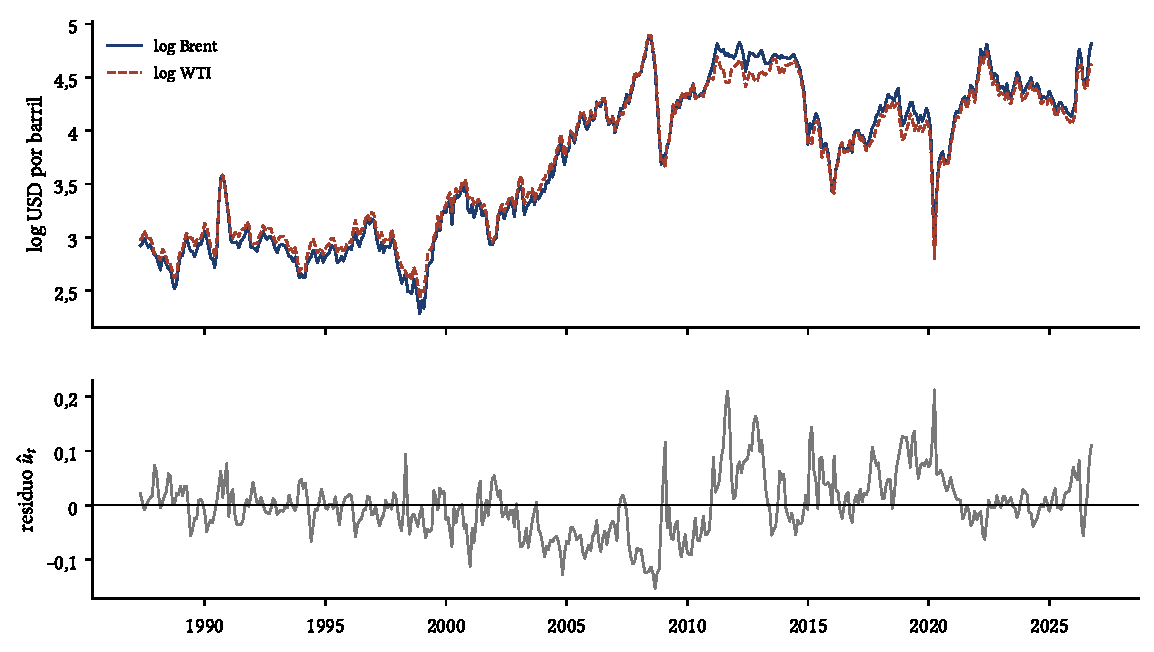
\includegraphics[width=0.92\linewidth]{graficos/cap11_ej01_brent_wti.pdf}
\caption{Arriba: logaritmos de los precios promedio mensuales del Brent y del WTI. Abajo: residuo de la regresión
de cointegración, que fluctúa alrededor de cero.}
\label{fig:brentwti}
\end{figure}

\begin{conclusion}
El Brent y el WTI están cointegrados: cada precio es un paseo aleatorio, pero la brecha entre ellos se corrige con
una vida media de unos cuatro meses.
\end{conclusion}
\end{ejresuelto}

\begin{ejresuelto}{Prueba de Johansen y VECM del petróleo}\label{ej:johansen}
\enunciado Elija el número de rezagos de un VAR en niveles con el BIC, aplique las pruebas de Johansen, estime el
VECM con $r=1$ e interprete $\hat\alpha$. Contraste $\beta=(1,-1)'$.

\solucion
\paso{Paso 1. Rezagos.} El BIC (y también el AIC) elige un VAR(3) en niveles, es decir, $k=2$ rezagos de las
diferencias en el VECM.

\paso{Paso 2. Rango.} Los autovalores son $\hat\lambda_1=0{,}06311$ y $\hat\lambda_2=0{,}00497$, con $n=471$:
\begin{align*}
  \lambda_{\text{traza}}(0) &= -471\bigl[\ln(1-0{,}06311)+\ln(1-0{,}00497)\bigr]\\
                            &= -471\,(-0{,}06519-0{,}00499)\\
                            &= 33{,}05,\\[4pt]
  \lambda_{\text{traza}}(1) &= -471\ln(1-0{,}00497)=2{,}35 .
\end{align*}
\begin{center}\small
\begin{tabular}{@{}lrrrr@{}}
\toprule
$H_0$ & Traza & VC 95\,\% & Máximo autovalor & VC 95\,\% \\
\midrule
$r=0$     & 33,05 & 15,49 & 30,70 & 14,26 \\
$r\le1$   & 2,35  & 3,84  & 2,35  & 3,84 \\
\bottomrule
\end{tabular}
\end{center}
Se rechaza $r=0$ y no se rechaza $r\le1$: hay exactamente una relación de cointegración.

\paso{Paso 3. VECM.} Normalizando el primer elemento a uno, $\hat\beta=(1;\ -1{,}1119)$, y
\begin{align*}
  \hat\alpha_{\text{Brent}} &= 0{,}0342\quad(t=0{,}40),\\
  \hat\alpha_{\text{WTI}}   &= 0{,}1664\quad(t=2{,}03).
\end{align*}
Solo el WTI corrige el desequilibrio: cuando el Brent está caro respecto del WTI, es el WTI el que sube al mes
siguiente. El Brent es débilmente exógeno, es decir, el precio de referencia que lidera. Es coherente con el
papel del Brent como marcador internacional, que fija el precio de dos tercios del crudo comerciado en el mundo.

\paso{Paso 4. Persistencia.} Por la Proposición~\ref{prop:ajustevecm}, aplicada como aproximación a un modelo con
rezagos:
\begin{align*}
  1+\hat\beta'\hat\alpha &= 1+1\times0{,}0342+(-1{,}1119)\times0{,}1664\\
                         &= 1+0{,}0342-0{,}1850\\
                         &= 0{,}8492,
\end{align*}
con una vida media de $\ln0{,}5/\ln0{,}8492=4{,}2$ meses, similar a la del Ejercicio~\ref{ej:eg}.

\paso{Paso 5. ¿Relación uno a uno?} Con $H=(1,-1)'$, el autovalor restringido es $0{,}0175$ y $LR=22{,}39$
($p=2{,}2\times10^{-6}$): se rechaza que $\beta=(1,-1)'$. En logaritmos, una relación uno a uno diría que el WTI
cuesta siempre la misma \emph{proporción} del Brent; los datos dicen que no, y el Ejercicio~\ref{ej:regimen}
muestra por qué.

\codigoweb{cap11_ej02}
\salidaR{cap11_ej02_R.txt}
\lectura{cap11_ej02}

\RvsPy Nuestra función \texttt{johansen} reproduce exactamente la función \texttt{coint\_johansen} de
\texttt{statsmodels}, llamada con los argumentos \texttt{(L, 0, 2)}, donde el \texttt{0} indica constante sin
restringir. El VECM coincide en $\hat\alpha$ y $\hat\beta$ con la clase \texttt{VECM} de \texttt{statsmodels}
con la opción \texttt{deterministic="co"}. Los errores estándar de $\hat\alpha$ difieren
levemente porque \texttt{statsmodels} divide la suma de cuadrados de los residuos entre $n$ y nosotros entre
$n-q$. En R, el número de rezagos elegido por \texttt{seleccion} conserva el nombre de la columna
(\texttt{"p"}) y ese nombre se propaga a los resultados; \texttt{unname} lo elimina.

\begin{figure}[ht]
\centering
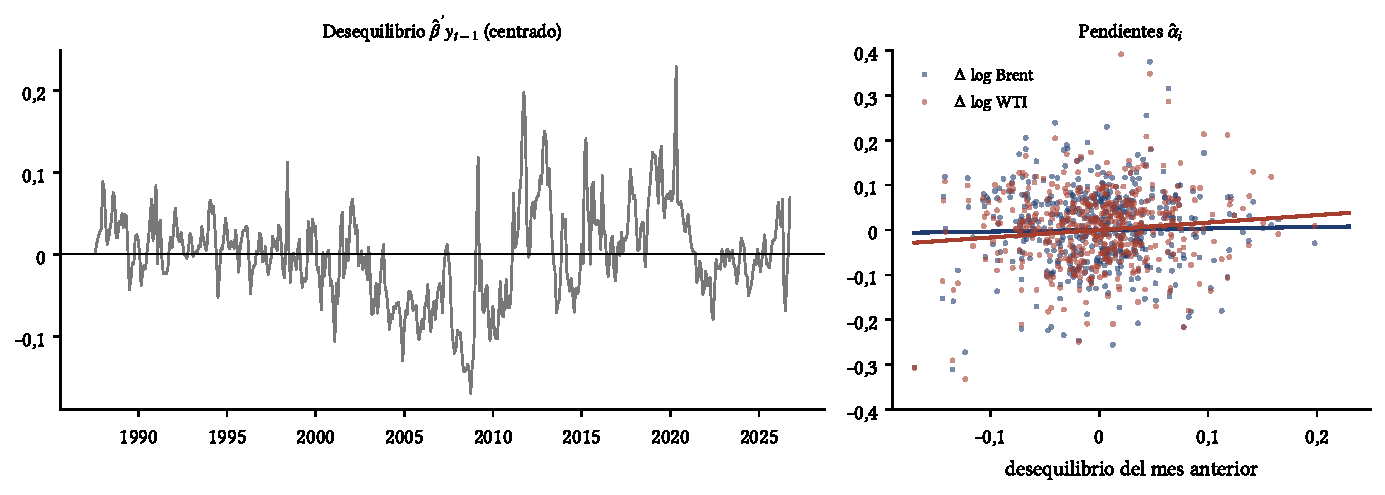
\includegraphics[width=\linewidth]{graficos/cap11_ej02_vecm.pdf}
\caption{Izquierda: desequilibrio estimado $\hat\beta'\mathbf y_{t-1}$, centrado. Derecha: cambio mensual de cada
precio frente al desequilibrio del mes anterior; las rectas tienen pendiente $\hat\alpha_i$, casi plana para el
Brent y positiva para el WTI.}
\label{fig:vecmpetro}
\end{figure}

\begin{conclusion}
Hay una relación de largo plazo entre el Brent y el WTI, y es el WTI el que se ajusta a ella. Pero la relación no es
de uno a uno en logaritmos durante toda la muestra.
\end{conclusion}
\end{ejresuelto}

\begin{ejresuelto}{El diferencial WTI-Brent y el cambio de régimen de 2011}\label{ej:regimen}
\enunciado Defina el diferencial $s_t=100(W_t-B_t)$, el precio del WTI respecto del Brent en porcentaje. Compare su
media y su estacionariedad, y las pruebas de Johansen, antes y después de enero de 2011.

\solucion
\paso{Paso 1. Dos regímenes.}
\begin{center}\small
\begin{tabular}{@{}lrrrrrr@{}}
\toprule
Período & $T$ & Media de $s_t$ & ADF de $s_t$ & Traza $r=0$ & $\hat\beta_{\text{WTI}}$ & $LR$: $\beta=(1,-1)'$ \\
\midrule
1987--2010 & 284 & 5,72 & $-2{,}66$ & 46,53 & $-1{,}048$ & 25,28 \\
2011--2026 & 190 & $-7{,}99$ & $-3{,}87$ & 22,88 & $-1{,}114$ & 6,12 \\
Completa   & 474 & 0,22 & $-1{,}74$ & 33,05 & $-1{,}112$ & 22,39 \\
\bottomrule
\end{tabular}
\end{center}
Hasta 2010 el WTI, un crudo más liviano y dulce, cotizaba en promedio 5,7\,\% por \emph{encima} del Brent. Desde
2011 cotiza 8,0\,\% por \emph{debajo}. En 2011--2013 la brecha promedió $-14{,}6$\,\% y llegó a $-27{,}7$\,\% en
septiembre de 2011 (Figura~\ref{fig:diferencial}). El aumento de la producción de crudo de esquisto en EE.\,UU.\
saturó la capacidad de almacenamiento y de oleoductos en Cushing (Oklahoma), donde se entrega el WTI, mientras que
el Brent seguía reflejando el mercado mundial. Cuando se construyeron nuevos oleoductos hacia la costa del
Golfo, la brecha se redujo, pero no volvió a su nivel anterior.

\paso{Paso 2. Lo que el cambio de media hace a las pruebas.} En la muestra completa el diferencial \emph{no} es
estacionario según la ADF ($-1{,}74$): una serie que fluctúa alrededor de dos medias distintas se parece a un
paseo aleatorio. Dentro de cada régimen la ADF es más negativa ($-2{,}66$, significativa al 10\,\% pero no al 5\,\%, y $-3{,}87$,
significativa al 1\,\%). Johansen encuentra cointegración en los tres casos, pero en la muestra completa lo hace
con $\hat\beta_{\text{WTI}}=-1{,}11$, lejos de uno: el $\beta$ se desvía para absorber el cambio de nivel.

\paso{Paso 3. Implicaciones.} Una relación de cointegración puede romperse por cambios estructurales en el
mercado. Con quiebres, las pruebas de raíz unitaria sobre el diferencial pierden potencia (como con el Brent en
el Capítulo~\ref{cap:raiz}) y el vector estimado se distorsiona. Para estos casos existen pruebas de cointegración
con quiebre endógeno, como la de Gregory y Hansen (1996).

\codigoweb{cap11_ej03}
\salidaR{cap11_ej03_R.txt}
\lectura{cap11_ej03}

\RvsPy Las submuestras se seleccionan comparando cadenas de fecha (\texttt{"2010-12"}), lo que funciona en los dos
lenguajes porque el formato \texttt{AAAA-MM} se ordena alfabéticamente igual que cronológicamente.

\begin{figure}[ht]
\centering
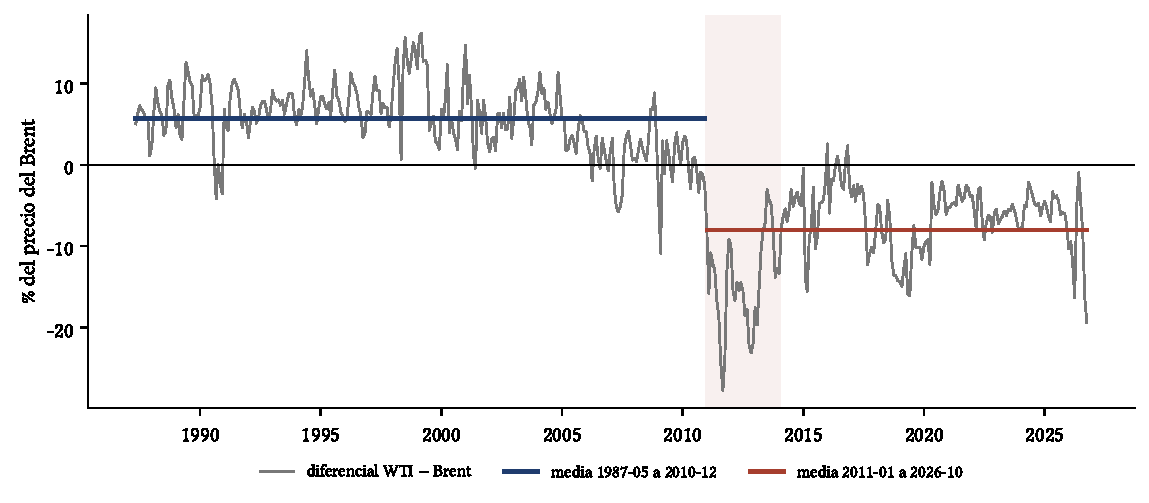
\includegraphics[width=0.92\linewidth]{graficos/cap11_ej03_diferencial.pdf}
\caption{Diferencial entre el WTI y el Brent en porcentaje, con la media de cada régimen. La franja sombreada marca
2011--2013, cuando la congestión en Cushing hundió el precio del WTI.}
\label{fig:diferencial}
\end{figure}

\begin{conclusion}
La ley de un solo precio entre el Brent y el WTI se cumple dentro de cada régimen, pero con un diferencial de
equilibrio que cambió de signo en 2011. Ignorar el quiebre lleva a un vector de cointegración distorsionado y a
pruebas engañosas sobre el diferencial.
\end{conclusion}
\end{ejresuelto}

\begin{ejresuelto}{El modelo de valor presente: precios, dividendos y utilidades}\label{ej:vp}
\enunciado Según el modelo de valor presente con tasa de descuento constante, el precio de una acción es
proporcional a sus dividendos esperados, y $\log(D_t/P_t)$ debería ser estacionario (Campbell y Shiller, 1987).
Con datos anuales reales del S\&P 500 (1871--2023), contraste la cointegración entre $\log P$ y $\log D$, y entre
$\log P$ y $\log E$ (utilidades).

\solucion
\paso{Paso 1. Raíces unitarias.}
\begin{center}\small
\begin{tabular}{@{}lrrrrr@{}}
\toprule
 & $\log P$ & $\log D$ & $\log E$ & $\log(D/P)$ & $\log(E/P)$ \\
\midrule
ADF ($t$) & $-0{,}31$ & $-0{,}43$ & 0,70 & $-1{,}41$ & $-4{,}66$ \\
\bottomrule
\end{tabular}
\end{center}
Los tres niveles son I(1). La razón utilidad/precio es claramente estacionaria, pero la razón dividendo/precio
no lo es.

\paso{Paso 2. Johansen.}
\begin{center}\small
\begin{tabular}{@{}lrrrrr@{}}
\toprule
Par & Traza $r=0$ & $\hat\beta$ & $t(\hat\alpha_P)$ & $t(\hat\alpha_X)$ & $LR$: $\beta=(1,-1)'$ \\
\midrule
$P$ y $D$ ($k=1$) & 21,21 & $(1;\ -1{,}720)$ & $-0{,}96$ & 4,39 & 17,51 \\
$P$ y $E$ ($k=0$) & 33,32 & $(1;\ -1{,}285)$ & 0,19 & 5,66 & 10,91 \\
\bottomrule
\end{tabular}
\end{center}
En ambos pares la traza rechaza $r=0$ (valor crítico 15,49), pero $\beta=(1,-1)'$ se rechaza también. Y quien
corrige el desequilibrio no es el precio, sino los dividendos y las utilidades ($\hat\alpha_X$ significativos,
$\hat\alpha_P$ no): cuando los precios están altos respecto de los dividendos, son los dividendos los que tienden a
subir después, no los precios los que bajan.

\paso{Paso 3. ¿Por qué no es estacionario $\log(D/P)$?} La razón dividendo/precio pasó de 5,86\,\% en 1871 a
1,70\,\% en 2023 (Figura~\ref{fig:vp}). Parte de la caída se debe a un cambio en la política de pagos: las empresas
repartían en promedio el 70,2\,\% de sus utilidades como dividendos entre 1871 y 1950, pero solo el 48,9\,\% entre
1990 y 2023, porque hoy devuelven efectivo a sus accionistas sobre todo recomprando acciones. Las utilidades no
tienen ese problema, y $\log(E/P)$ sí resulta estacionario.

\codigoweb{cap11_ej04}
\salidaR{cap11_ej04_R.txt}
\lectura{cap11_ej04}

\RvsPy Con $k=0$ no hay rezagos de las diferencias y la matriz de regresores auxiliares contiene solo la
constante. En R, \texttt{cbind(1, NULL)} produce una matriz $1\times1$ y no un vector columna de unos, lo que
rompía los productos matriciales; la función usa \texttt{matrix(1, n, 1)}. En Python, \texttt{np.column\_stack}
con una sola columna no tiene ese problema.

\begin{figure}[ht]
\centering
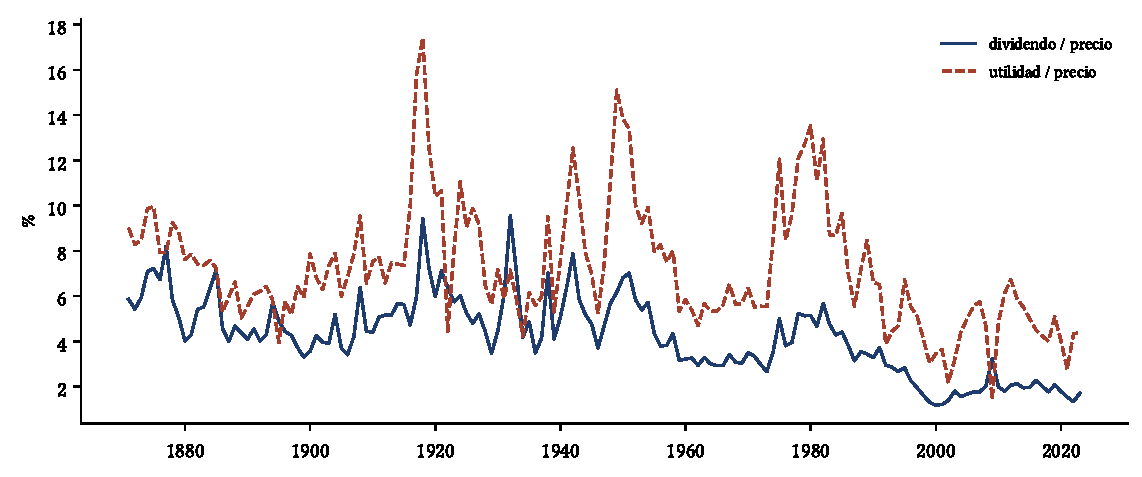
\includegraphics[width=0.92\linewidth]{graficos/cap11_ej04_valor_presente.pdf}
\caption{Razones dividendo/precio y utilidad/precio del S\&P 500 (enero de cada año, 1871--2023). La primera tiene
una tendencia descendente; la segunda fluctúa alrededor de un nivel estable.}
\label{fig:vp}
\end{figure}

\begin{conclusion}
Precios, dividendos y utilidades comparten una tendencia de largo plazo, pero la relación no es la proporcional
que supone el modelo de valor presente más simple, sobre todo para los dividendos. Y el ajuste lo hacen los
fundamentos, no los precios: los precios altos anuncian dividendos más altos, no caídas de precio, un resultado
que debe leerse con cautela porque los cambios en la política de pagos rompen la estacionariedad de $D/P$.
\end{conclusion}
\end{ejresuelto}

\begin{ejresuelto}{¿Ayuda la corrección de errores a pronosticar?}\label{ej:vecmpron}
\enunciado Pronostique el cambio mensual de $\log$ Brent y $\log$ WTI desde enero de 2005, con ventana creciente,
usando un paseo aleatorio, un VAR(2) en diferencias y el VECM con $k=2$ y $r=1$ (reestimando $\beta$ en cada mes).
Compare la raíz del error cuadrático medio (RECM) y aplique la prueba de Clark y West del VAR en diferencias
(anidado, con $\alpha=0$) frente al VECM.

\solucion
\paso{Paso 1. Errores.} Con 262 pronósticos:
\begin{center}\small
\begin{tabular}{@{}lrrr@{}}
\toprule
RECM (\%) & Paseo aleatorio & VAR en diferencias & VECM \\
\midrule
Brent & 10,776 & 10,415 & 10,546 \\
WTI   & 10,728 & 10,504 & 10,537 \\
\bottomrule
\end{tabular}
\end{center}
Los dos modelos dinámicos superan al paseo aleatorio (en parte por el efecto Working que introduce promediar los
precios), pero el VECM no supera al VAR en diferencias.

\paso{Paso 2. Clark y West.} Para el Brent, $t=-1{,}73$ ($p=0{,}96$); para el WTI, $t=0{,}11$ ($p=0{,}46$). La
corrección de errores no mejora los pronósticos a un mes, y su $R^2$ fuera de muestra respecto del VAR en
diferencias es negativo ($-2{,}54$\,\% y $-0{,}63$\,\%).

\paso{Paso 3. ¿Por qué?} La Figura~\ref{fig:vecmpron} muestra que el VECM acumula casi toda su desventaja en dos
episodios: el derrumbe de fines de 2008 y la anomalía de abril de 2020. En ambos, el desequilibrio fue enorme y el
modelo predijo una corrección fuerte que no llegó al mes siguiente. Además, $\hat\beta$ cambia con el quiebre de
2011. Christoffersen y Diebold (1998) muestran que la cointegración ayuda sobre todo a pronosticar a horizontes
largos, y no tanto a un mes, cuando dominan los choques de corto plazo.

\codigoweb{cap11_ej05}
\salidaR{cap11_ej05_R.txt}
\lectura{cap11_ej05}

\RvsPy El pronóstico del VECM es el producto del vector $(\hat\beta'\mathbf y_{t-1},\,1,\,\Delta\mathbf y_{t-1}',\,
\Delta\mathbf y_{t-2}')$ por la matriz de coeficientes estimada; el del VAR en diferencias usa el mismo vector sin el
primer elemento. Como Python indexa desde cero, el cambio del mes $t$ es \texttt{dYall[t-1]}; en R es
\texttt{diff(L)[t - 1, ]} con $t$ contado desde uno. Ambos dan idénticos resultados.

\begin{figure}[ht]
\centering
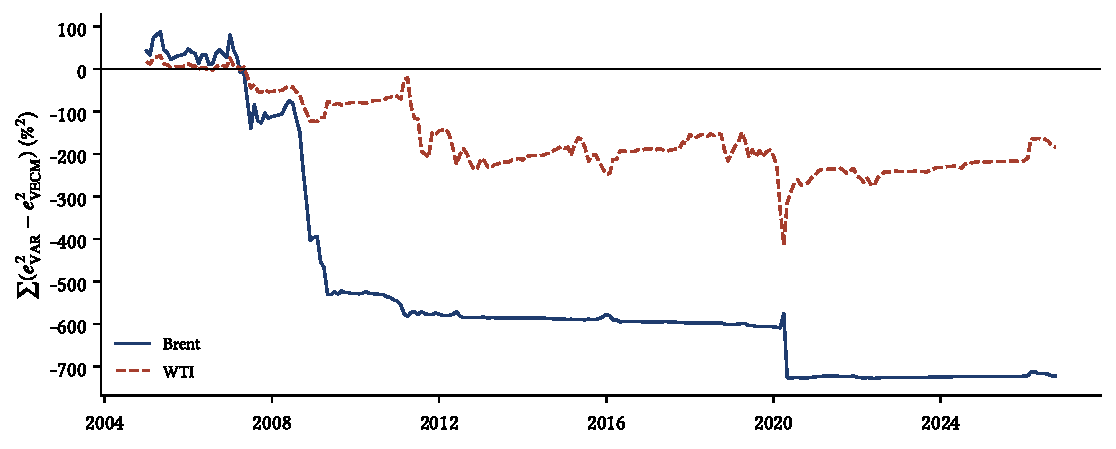
\includegraphics[width=0.88\linewidth]{graficos/cap11_ej05_pronostico.pdf}
\caption{Diferencia acumulada entre los errores cuadráticos del VAR en diferencias y los del VECM. Una curva que
baja indica que el VECM pronostica peor; las caídas se concentran en 2008 y 2020.}
\label{fig:vecmpron}
\end{figure}

\begin{conclusion}
Que dos precios estén cointegrados no garantiza que el modelo de corrección de errores pronostique mejor a corto
plazo. Con quiebres estructurales y choques extremos, el término de corrección puede incluso empeorar el
pronóstico.
\end{conclusion}
\end{ejresuelto}

% ---------------------------------------------------------------------
\section{Ejercicios propuestos}
% ---------------------------------------------------------------------

\begin{enumerate}[label=\textbf{\thechapter.\arabic*},leftmargin=*,itemsep=6pt]
  \item Escriba el VECM de un VAR(3) y exprese $\Gamma_1$ y $\Gamma_2$ en función de $A_1$, $A_2$ y $A_3$.
  \textit{Respuesta: $\Gamma_1=-(A_2+A_3)$, $\Gamma_2=-A_3$.}

  \item En un VECM bivariado sin rezagos con $\beta=(1,-1)'$ y $\alpha=(-0{,}1;\ 0{,}1)$, calcule el coeficiente
  autorregresivo del desequilibrio, su vida media y el nivel final tras un choque $\mathbf y_0=(1,0)'$.
  \textit{Respuesta: $0{,}8$; $3{,}1$ períodos; $0{,}5$.}

  \item Demuestre que si $\Pi=\alpha\beta'$ con $\alpha$ y $\beta$ de dimensión $K\times r$, entonces
  $\operatorname{rango}(\Pi)\le r$.

  \item Con autovalores $\hat\lambda=(0{,}10;\ 0{,}02)$ y $n=300$, calcule los estadísticos de la traza y del máximo
  autovalor y decida el rango con los valores críticos del texto. \textit{Respuesta: traza $37{,}67$ y $6{,}06$;
  máximo $31{,}61$ y $6{,}06$; rango 2, es decir, ambas series serían estacionarias.}

  \item \emph{(Simulación.)} Simule 2\,000 pares de paseos aleatorios independientes con $T=200$, aplique la prueba
  de Engle y Granger y compare la frecuencia de rechazos con los valores críticos de Dickey-Fuller ($-2{,}86$) y de
  MacKinnon ($-3{,}37$ para $T=200$). ¿Cuál tiene el tamaño correcto?

  \item \emph{(Con datos del BCRP.)} Contraste la cointegración entre el tipo de cambio sol/dólar y el índice de
  precios relativos Perú/EE.\,UU. (paridad del poder de compra). ¿Qué variable corrige?

  \item \emph{(Con datos.)} Repita el Ejercicio~\ref{ej:johansen} solo para 2011--2026 e interprete $\hat\alpha$.
  ¿Sigue siendo el Brent débilmente exógeno?

  \item \emph{(Con datos de Yahoo Finance.)} Descargue los precios diarios de dos acciones del mismo sector (por
  ejemplo, dos bancos). Contraste la cointegración en 2015--2020 y use el residuo estandarizado como señal de una
  estrategia de \emph{pairs trading} en 2021--2025. ¿Se mantiene la relación fuera de la muestra?
\end{enumerate}

% ---------------------------------------------------------------------
\section{Resumen de fórmulas}
% ---------------------------------------------------------------------

\begin{table}[H]
\centering\small
\begin{tabular}{@{}ll@{}}
\toprule
Concepto & Fórmula \\
\midrule
VECM & $\Delta\mathbf y_t=\mathbf c+\alpha\beta'\mathbf y_{t-1}+\sum_{i=1}^{p-1}\Gamma_i\Delta\mathbf y_{t-i}+\mathbf u_t$ \\
Matrices & $\Pi=-(I-\sum_jA_j)=\alpha\beta'$;\quad $\Gamma_i=-\sum_{j>i}A_j$ \\
Desequilibrio & $z_t=\beta'\mathbf y_t$;\quad persistencia $1+\beta'\alpha$ (sin rezagos) \\
Engle-Granger & ADF sin constante sobre $\hat u_t$;\quad VC 5\,\%: $-3{,}336-6{,}11/T-6{,}82/T^2$ \\
Johansen & autovalores de $S_{11}^{-1}S_{10}S_{00}^{-1}S_{01}$ \\
Traza & $-n\sum_{i=r+1}^{K}\ln(1-\hat\lambda_i)$ \\
Máximo autovalor & $-n\ln(1-\hat\lambda_{r+1})$ \\
Restricción $\beta=H\varphi$ & $n[\ln(1-\tilde\lambda_1)-\ln(1-\hat\lambda_1)]\sim\chi^2_{K-s}$ \\
\bottomrule
\end{tabular}
\caption{Fórmulas principales del Capítulo 11.}
\end{table}

\section*{Referencias}
\begin{itemize}[leftmargin=*]
  \item Campbell, J. Y. y Shiller, R. J. (1987). Cointegration and tests of present value models. \emph{Journal of
        Political Economy}, 95(5), 1062--1088.
  \item Christoffersen, P. F. y Diebold, F. X. (1998). Cointegration and long-horizon forecasting. \emph{Journal of
        Business \& Economic Statistics}, 16(4), 450--458.
  \item Engle, R. F. y Granger, C. W. J. (1987). Co-integration and error correction: Representation, estimation,
        and testing. \emph{Econometrica}, 55(2), 251--276.
  \item Gregory, A. W. y Hansen, B. E. (1996). Residual-based tests for cointegration in models with regime
        shifts. \emph{Journal of Econometrics}, 70(1), 99--126.
  \item Johansen, S. (1988). Statistical analysis of cointegration vectors. \emph{Journal of Economic Dynamics and
        Control}, 12(2--3), 231--254.
  \item Johansen, S. (1991). Estimation and hypothesis testing of cointegration vectors in Gaussian vector
        autoregressive models. \emph{Econometrica}, 59(6), 1551--1580.
  \item MacKinnon, J. G. (2010). Critical values for cointegration tests. Queen's Economics Department Working
        Paper 1227.
  \item MacKinnon, J. G., Haug, A. A. y Michelis, L. (1999). Numerical distribution functions of likelihood ratio
        tests for cointegration. \emph{Journal of Applied Econometrics}, 14(5), 563--577.
\end{itemize}

% =====================================================================
%  Capítulo 12. Volatilidad multivariada y correlaciones dinámicas
% =====================================================================
\chapter[Correlaciones dinámicas]{Volatilidad multivariada: EWMA, correlación condicional constante y DCC}\label{cap:dcc}

\section*{Objetivos de aprendizaje}
Al terminar este capítulo, el lector podrá:
\begin{enumerate}[label=\arabic*.,leftmargin=*]
  \item Explicar por qué modelar matrices de covarianza condicionales es difícil y cómo lo resuelven los modelos
        EWMA, CCC y DCC.
  \item Demostrar que la verosimilitud del DCC se separa en una parte de volatilidad y otra de correlación, y
        estimar el modelo en dos etapas.
  \item Usar las covarianzas condicionales para construir carteras de mínima varianza y evaluarlas fuera de
        muestra.
  \item Distinguir el aumento de correlación por contagio del que produce mecánicamente un aumento de
        volatilidad (Forbes y Rigobon).
\end{enumerate}

\section*{Motivación}
La diversificación descansa en una cifra: la correlación entre los activos. Si es baja, combinar activos reduce
el riesgo; si sube justo cuando los mercados caen, la protección desaparece cuando más se necesita. Los
Capítulos~\ref{cap:garch} y~\ref{cap:asimetria} mostraron que las volatilidades cambian en el tiempo; este
capítulo muestra que las correlaciones también. La correlación entre el petróleo y las acciones de EE.\,UU.,
por ejemplo, era casi nula antes de 2008 y luego se volvió claramente positiva. Gestionar carteras, calcular
el riesgo de una posición cubierta o medir el contagio entre mercados exige modelar la matriz de covarianzas
completa.

\paragraph{Datos del capítulo.} Rendimientos logarítmicos diarios del S\&P 500 y del Nasdaq Composite (Yahoo
Finance) y del Brent (EIA), en los 4\,615 días en que los tres cotizaron entre enero de 1999 y diciembre de 2018.
Cuando un mercado cierra y otro no, el rendimiento del día siguiente abarca dos días; con datos diarios de
mercados de distintos países esa falta de sincronía es inevitable y tiende a reducir las correlaciones medidas.

% ---------------------------------------------------------------------
\section{La matriz de covarianzas condicional}
% ---------------------------------------------------------------------

Sea $\boldsymbol\varepsilon_t=\mathbf r_t-\boldsymbol\mu$ el vector de $K$ innovaciones, con
\[
  \E[\boldsymbol\varepsilon_t\mid\mathcal F_{t-1}]=\mathbf 0,\qquad
  \Var(\boldsymbol\varepsilon_t\mid\mathcal F_{t-1})=H_t .
\]
Un modelo para $H_t$ debe cumplir dos requisitos: que $H_t$ sea definida positiva en todo momento (de lo
contrario alguna cartera tendría varianza negativa) y que el número de parámetros no explote con $K$. La
generalización directa del GARCH, en la que cada elemento de $H_t$ depende de todos los productos
$\varepsilon_{i,t-1}\varepsilon_{j,t-1}$, tiene del orden de $K^4$ parámetros: con $K=10$, más de 6\,000. Los
modelos de este capítulo resuelven el problema separando volatilidades y correlaciones.

\subsection{EWMA multivariado}

La extensión de RiskMetrics aplica la misma media móvil exponencial a cada varianza y covarianza:
\[
  H_t=\lambda H_{t-1}+(1-\lambda)\,\boldsymbol\varepsilon_{t-1}\boldsymbol\varepsilon_{t-1}',\qquad\lambda=0{,}94 .
\]
Como $\boldsymbol\varepsilon\boldsymbol\varepsilon'$ es semidefinida positiva, $H_t$ es definida positiva si
$H_{t-1}$ lo es. No requiere estimación, pero impone la misma persistencia a todas las varianzas y covarianzas,
y no tiene nivel de largo plazo (es un IGARCH).

\subsection{Correlación condicional constante (CCC)}

Bollerslev (1990) propuso descomponer
\[
  H_t=D_tRD_t,\qquad D_t=\operatorname{diag}(\sigma_{1t},\dots,\sigma_{Kt}),
\]
donde cada $\sigma_{it}^2$ sigue un GARCH univariado y $R$ es una matriz de correlaciones constante. La covarianza
$h_{ij,t}=\rho_{ij}\sigma_{it}\sigma_{jt}$ cambia solo porque cambian las volatilidades.

\subsection{Correlación condicional dinámica (DCC)}

\begin{definicion}[DCC(1,1); Engle, 2002]
Sea $\mathbf z_t=D_t^{-1}\boldsymbol\varepsilon_t$ el vector de residuos estandarizados de los GARCH univariados
y $\bar Q=\frac1T\sum_t\mathbf z_t\mathbf z_t'$. Con $a,b\ge0$ y $a+b<1$,
\begin{align*}
  Q_t &= (1-a-b)\,\bar Q+a\,\mathbf z_{t-1}\mathbf z_{t-1}'+b\,Q_{t-1},\\
  R_t &= \operatorname{diag}(Q_t)^{-1/2}\,Q_t\,\operatorname{diag}(Q_t)^{-1/2},\\
  H_t &= D_tR_tD_t .
\end{align*}
\end{definicion}

La matriz $Q_t$ es un GARCH(1,1) escalar para los productos de residuos estandarizados, con nivel de largo plazo
$\bar Q$ (\emph{correlation targeting}). Su diagonal no es exactamente uno, así que se reescala para obtener una
matriz de correlaciones. Con solo dos parámetros, sea cual sea $K$, el modelo permite que todas las correlaciones
cambien, aunque con la misma dinámica.

\begin{proposicion}[$R_t$ es una matriz de correlaciones definida positiva]\label{prop:dccpd}
Si $\bar Q$ y $Q_0$ son definidas positivas, $a,b\ge0$ y $a+b<1$, entonces $Q_t$ es definida positiva para todo
$t$, y $R_t$ es una matriz de correlaciones definida positiva.
\end{proposicion}

\begin{proof}
Por inducción. Supongamos $Q_{t-1}$ definida positiva. Para todo $\mathbf x\ne\mathbf 0$:
\begin{align*}
  \mathbf x'Q_t\mathbf x &= (1-a-b)\,\mathbf x'\bar Q\mathbf x+a\,\mathbf x'\mathbf z_{t-1}\mathbf z_{t-1}'\mathbf x+b\,\mathbf x'Q_{t-1}\mathbf x\\
                         &= (1-a-b)\,\mathbf x'\bar Q\mathbf x+a\,(\mathbf z_{t-1}'\mathbf x)^2+b\,\mathbf x'Q_{t-1}\mathbf x .
\end{align*}
El primer término es estrictamente positivo porque $1-a-b>0$ y $\bar Q$ es definida positiva; los otros dos son
no negativos. Luego $\mathbf x'Q_t\mathbf x>0$. Para $R_t$, sea $S=\operatorname{diag}(Q_t)^{-1/2}$, que es diagonal
con elementos positivos, y $\mathbf y=S\mathbf x\ne\mathbf 0$:
\begin{align*}
  \mathbf x'R_t\mathbf x &= \mathbf x'SQ_tS\mathbf x\\
                         &= (S\mathbf x)'Q_t(S\mathbf x)\\
                         &= \mathbf y'Q_t\mathbf y>0 .
\end{align*}
Su diagonal es $[R_t]_{ii}=q_{ii,t}/\sqrt{q_{ii,t}q_{ii,t}}=1$. Una matriz simétrica definida positiva con unos
en la diagonal es una matriz de correlaciones: por la desigualdad de Cauchy-Schwarz, sus elementos fuera de la
diagonal están entre $-1$ y $1$.
\end{proof}

\paragraph{Curva de impacto de la correlación.} ¿Cómo responde la correlación a las noticias? Si hoy dos activos
reciben choques del mismo signo, $z_{1}z_{2}>0$ y $q_{12}$ sube; si son de signo opuesto, baja. La
Figura~\ref{fig:dccteoria} (derecha) lo muestra con $a=0{,}05$, $b=0{,}93$ y una correlación de partida de
$0{,}3$: dos choques de $+2$ desviaciones estándar la elevan a $0{,}42$; choques de $+2$ y $-2$ la reducen a $0{,}07$.
Los contornos tienen forma de silla de montar: la correlación sube en los cuadrantes primero y tercero, y baja en
los otros dos.

% ---------------------------------------------------------------------
\section{Estimación en dos etapas}
% ---------------------------------------------------------------------

\begin{proposicion}[Separación de la verosimilitud]\label{prop:dccll}
Con innovaciones normales, la log-verosimilitud de $\boldsymbol\varepsilon_t\mid\mathcal F_{t-1}\sim N(\mathbf 0,H_t)$
con $H_t=D_tR_tD_t$ se separa en
\begin{align*}
  \ell &= \ell_V+\ell_C,\\
  \ell_V &= -\frac12\sum_{t}\sum_{i=1}^{K}\Bigl[\ln(2\pi)+\ln\sigma_{it}^2+\frac{\varepsilon_{it}^2}{\sigma_{it}^2}\Bigr],\\
  \ell_C &= -\frac12\sum_{t}\Bigl[\ln|R_t|+\mathbf z_t'R_t^{-1}\mathbf z_t-\mathbf z_t'\mathbf z_t\Bigr].
\end{align*}
$\ell_V$ es la suma de las verosimilitudes de $K$ GARCH univariados y solo $\ell_C$ depende de $(a,b)$.
\end{proposicion}

\begin{proof}
La densidad normal multivariada da
\begin{align*}
  \ell_t &= -\frac12\Bigl[K\ln(2\pi)+\ln|H_t|+\boldsymbol\varepsilon_t'H_t^{-1}\boldsymbol\varepsilon_t\Bigr].
\end{align*}
El determinante de un producto es el producto de los determinantes, y $|D_t|=\prod_i\sigma_{it}$:
\begin{align*}
  \ln|H_t| &= \ln|D_t|+\ln|R_t|+\ln|D_t|\\
           &= \sum_{i=1}^{K}\ln\sigma_{it}^2+\ln|R_t| .
\end{align*}
Para la forma cuadrática, con $H_t^{-1}=D_t^{-1}R_t^{-1}D_t^{-1}$ y $\mathbf z_t=D_t^{-1}\boldsymbol\varepsilon_t$:
\begin{align*}
  \boldsymbol\varepsilon_t'H_t^{-1}\boldsymbol\varepsilon_t &= (D_t^{-1}\boldsymbol\varepsilon_t)'R_t^{-1}(D_t^{-1}\boldsymbol\varepsilon_t)\\
                                                           &= \mathbf z_t'R_t^{-1}\mathbf z_t .
\end{align*}
Sumamos y restamos $\mathbf z_t'\mathbf z_t=\sum_i\varepsilon_{it}^2/\sigma_{it}^2$:
\begin{align*}
  \ell_t &= -\frac12\Bigl[K\ln(2\pi)+\sum_i\ln\sigma_{it}^2+\ln|R_t|+\mathbf z_t'R_t^{-1}\mathbf z_t\Bigr]\\
         &= -\frac12\Bigl[K\ln(2\pi)+\sum_i\ln\sigma_{it}^2+\mathbf z_t'\mathbf z_t\Bigr]
            -\frac12\Bigl[\ln|R_t|+\mathbf z_t'R_t^{-1}\mathbf z_t-\mathbf z_t'\mathbf z_t\Bigr]\\
         &= -\frac12\sum_{i=1}^{K}\Bigl[\ln(2\pi)+\ln\sigma_{it}^2+\frac{\varepsilon_{it}^2}{\sigma_{it}^2}\Bigr]
            -\frac12\Bigl[\ln|R_t|+\mathbf z_t'R_t^{-1}\mathbf z_t-\mathbf z_t'\mathbf z_t\Bigr].
\end{align*}
Sumando sobre $t$ se obtiene $\ell=\ell_V+\ell_C$. Restar $\mathbf z_t'\mathbf z_t$ en $\ell_C$ no cambia su
máximo respecto de $(a,b)$; solo hace que $\ell_C=0$ cuando $R_t=I$.
\end{proof}

La proposición justifica el procedimiento de Engle (2002): (1) estimar un GARCH univariado para cada serie y
calcular $\mathbf z_t$; (2) maximizar $\ell_C$ respecto de $(a,b)$ con $\bar Q$ fijo en su valor muestral. El
estimador es consistente, aunque menos eficiente que la máxima verosimilitud conjunta; los errores estándar de
la segunda etapa, si se calculan con la hessiana de $\ell_C$, ignoran la incertidumbre de la primera y tienden a
ser optimistas. El CCC es el caso $a=b=0$ con $R_t=R$; la razón de verosimilitudes $2(\ell_C^{\text{DCC}}-\ell_C^{\text{CCC}})$
mide la ganancia de dejar que la correlación cambie. Su distribución no es exactamente $\chi^2_2$, porque bajo
$a=0$ el parámetro $b$ no está identificado, pero una cifra muy grande deja poca duda.

% ---------------------------------------------------------------------
\section{Aplicaciones}
% ---------------------------------------------------------------------

\subsection{Cartera de mínima varianza}

\begin{proposicion}[Cartera de mínima varianza]\label{prop:minvar}
Con matriz de covarianzas $H$ definida positiva, los pesos que minimizan la varianza $\mathbf w'H\mathbf w$ sujeto a
$\mathbf w'\boldsymbol\iota=1$ (con $\boldsymbol\iota$ un vector de unos) son
\[
  \mathbf w^*=\frac{H^{-1}\boldsymbol\iota}{\boldsymbol\iota'H^{-1}\boldsymbol\iota},\qquad
  \mathbf w^{*\prime}H\mathbf w^*=\frac{1}{\boldsymbol\iota'H^{-1}\boldsymbol\iota}.
\]
\end{proposicion}

\begin{proof}
El lagrangiano es $\mathcal L=\mathbf w'H\mathbf w-\lambda(\mathbf w'\boldsymbol\iota-1)$. La condición de
primer orden da
\begin{align*}
  \frac{\partial\mathcal L}{\partial\mathbf w} &= 2H\mathbf w-\lambda\boldsymbol\iota=\mathbf 0,\\
  \mathbf w &= \frac\lambda2\,H^{-1}\boldsymbol\iota .
\end{align*}
La restricción fija $\lambda$:
\begin{align*}
  \boldsymbol\iota'\mathbf w &= \frac\lambda2\,\boldsymbol\iota'H^{-1}\boldsymbol\iota=1,\\
  \frac\lambda2 &= \frac{1}{\boldsymbol\iota'H^{-1}\boldsymbol\iota}.
\end{align*}
Sustituyendo se obtiene $\mathbf w^*$. Su varianza es
\begin{align*}
  \mathbf w^{*\prime}H\mathbf w^* &= \frac{\boldsymbol\iota'H^{-1}HH^{-1}\boldsymbol\iota}{(\boldsymbol\iota'H^{-1}\boldsymbol\iota)^2}\\
                                  &= \frac{\boldsymbol\iota'H^{-1}\boldsymbol\iota}{(\boldsymbol\iota'H^{-1}\boldsymbol\iota)^2}\\
                                  &= \frac{1}{\boldsymbol\iota'H^{-1}\boldsymbol\iota}.
\end{align*}
Es un mínimo porque $H$ es definida positiva.
\end{proof}

Con $H_t$ condicional, los pesos cambian cada día. La comparación de modelos de covarianza mediante la varianza
realizada de las carteras que generan es un criterio económico, no solo estadístico (Engle y Colacito, 2006): el
mejor modelo es el que produce la cartera menos riesgosa fuera de la muestra.

\subsection{Contagio y el sesgo de la correlación condicionada}

Que la correlación medida suba en una crisis no prueba que haya contagio. Forbes y Rigobon (2002) mostraron que
la correlación aumenta mecánicamente cuando aumenta la volatilidad del mercado de origen, aunque la relación
entre los mercados no cambie.

\begin{proposicion}[Sesgo de Forbes y Rigobon]\label{prop:forbes}
Sea $y=\beta x+e$ con $e$ no correlacionado con $x$ y $\beta$ y $\Var(e)$ iguales en calma y en crisis. Si en la
crisis la varianza de $x$ aumenta en un factor $1+\delta$, la correlación pasa de $\rho$ a
\[
  \rho_c=\rho\,\sqrt{\frac{1+\delta}{1+\delta\rho^2}} .
\]
Por tanto, la correlación en la crisis corregida por el sesgo es $\rho^*=\rho_c\big/\sqrt{1+\delta(1-\rho_c^2)}$.
\end{proposicion}

\begin{proof}
En calma, con $\sigma_x^2=\Var(x)$ y $\sigma_e^2=\Var(e)$:
\begin{align*}
  \rho^2 &= \frac{\Cov(x,y)^2}{\Var(x)\Var(y)}\\
         &= \frac{\beta^2\sigma_x^4}{\sigma_x^2(\beta^2\sigma_x^2+\sigma_e^2)}\\
         &= \frac{\beta^2\sigma_x^2}{\beta^2\sigma_x^2+\sigma_e^2}.
\end{align*}
Despejamos $\sigma_e^2$:
\begin{align*}
  \sigma_e^2 &= \beta^2\sigma_x^2\,\frac{1-\rho^2}{\rho^2}.
\end{align*}
En la crisis, $\sigma_x^2$ se convierte en $(1+\delta)\sigma_x^2$ y $\sigma_e^2$ no cambia:
\begin{align*}
  \rho_c^2 &= \frac{\beta^2(1+\delta)\sigma_x^2}{\beta^2(1+\delta)\sigma_x^2+\sigma_e^2}\\
           &= \frac{(1+\delta)}{(1+\delta)+(1-\rho^2)/\rho^2}\\
           &= \frac{(1+\delta)\rho^2}{(1+\delta)\rho^2+1-\rho^2}\\
           &= \frac{(1+\delta)\rho^2}{1+\delta\rho^2}.
\end{align*}
Tomando raíz (con el signo de $\beta$) se obtiene $\rho_c$. Para invertir la relación, despejamos $\rho^2$ de la
última igualdad:
\begin{align*}
  \rho_c^2(1+\delta\rho^2) &= (1+\delta)\rho^2,\\
  \rho_c^2 &= \rho^2\bigl[(1+\delta)-\delta\rho_c^2\bigr],\\
  \rho^2 &= \frac{\rho_c^2}{1+\delta(1-\rho_c^2)}. && \qedhere
\end{align*}
\end{proof}

La Figura~\ref{fig:dccteoria} (izquierda) muestra la magnitud del sesgo: si la varianza del mercado de origen se
cuadruplica ($\delta=3$), una correlación de $0{,}3$ se mide como
\begin{align*}
  \rho_c &= 0{,}3\sqrt{\frac{1+3}{1+3(0{,}09)}}\\
         &= 0{,}3\times\frac{2}{\sqrt{1{,}27}}\\
         &= 0{,}532,
\end{align*}
sin que haya cambiado nada en la relación entre los mercados. La corrección supone que todo el aumento de
volatilidad nace en $x$ y que no hay variables omitidas; si ambos mercados reciben a la vez un choque común,
la corrección es excesiva.

\begin{figure}[ht]
\centering
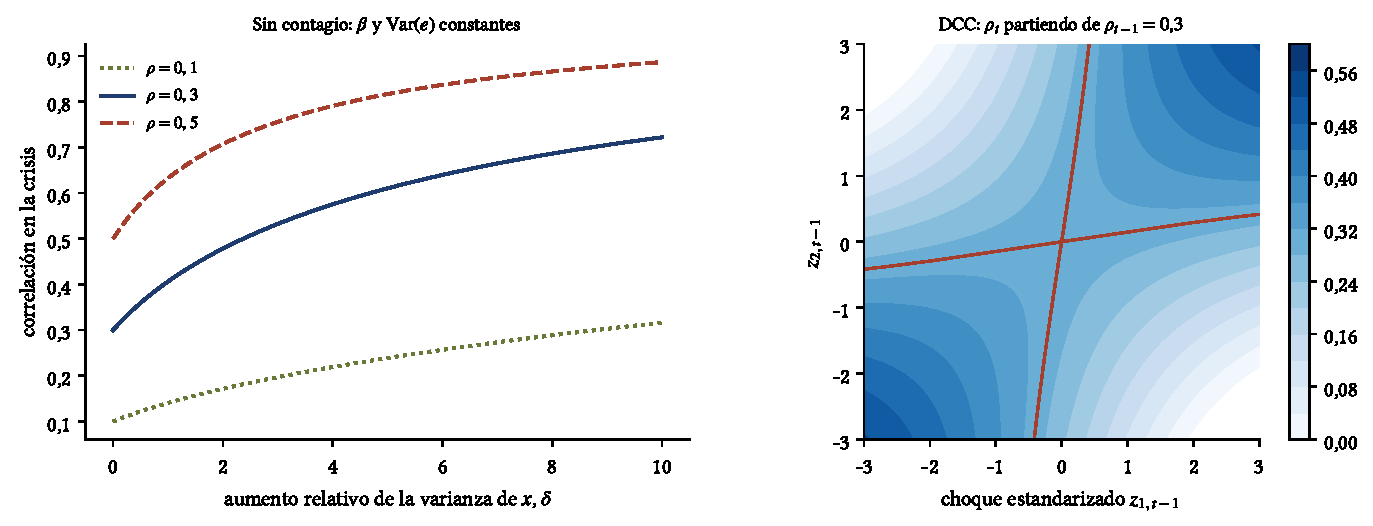
\includegraphics[width=\linewidth]{graficos/cap12_fig_teoria.pdf}
\caption{Izquierda: correlación medida en un período en que la varianza del mercado de origen aumenta un factor
$1+\delta$, sin contagio (Proposición~\ref{prop:forbes}). Derecha: correlación de mañana en un DCC con
$a=0{,}05$ y $b=0{,}93$ según los choques estandarizados de hoy; la línea roja marca los choques que la dejan en
$0{,}3$.}
\label{fig:dccteoria}
\end{figure}

% ---------------------------------------------------------------------
\section{Ejercicios resueltos}
% ---------------------------------------------------------------------

\begin{ejresuelto}{Correlaciones que cambian}\label{ej:corrmov}
\enunciado Calcule las correlaciones diarias entre el S\&P 500, el Nasdaq y el Brent en toda la muestra y por
subperíodos, y las correlaciones con una ventana móvil de 250 días y con EWMA ($\lambda=0{,}94$).

\solucion
\paso{Paso 1. Correlaciones incondicionales.} En toda la muestra, la correlación S\&P--Nasdaq es $0{,}885$ y la
S\&P--Brent, $0{,}139$. Pero por subperíodos:
\begin{center}\small
\begin{tabular}{@{}lrr@{}}
\toprule
Par & 1999--2007 & 2009--2018 \\
\midrule
S\&P--Brent  & 0,006 & 0,299 \\
S\&P--Nasdaq & 0,852 & 0,954 \\
\bottomrule
\end{tabular}
\end{center}
La correlación entre el petróleo y las acciones pasó de cero a $0{,}30$ después de la crisis financiera.

\paso{Paso 2. Correlaciones móviles.} Con EWMA, la correlación S\&P--Brent va de $-0{,}64$ (diciembre de 2004) a
$0{,}74$ (junio de 2012); con la ventana de 250 días, de $-0{,}25$ a $0{,}54$ (Figura~\ref{fig:corrmov}). La EWMA es
mucho más ruidosa: con $\lambda=0{,}94$ su ``memoria'' efectiva es de unos $1/(1-\lambda)\approx17$ días. La ventana
móvil es más suave, pero reacciona tarde y cambia bruscamente cuando una observación extrema sale de la ventana.

\codigoweb{cap12_ej01}
\salidaR{cap12_ej01_R.txt}
\lectura{cap12_ej01}

\RvsPy Las covarianzas EWMA se guardan en un arreglo tridimensional $T\times K\times K$: \texttt{array(0, c(T, K,
K))} en R y \texttt{np.empty((T, K, K))} en Python; \texttt{tcrossprod(e)} de R y \texttt{np.outer(e, e)} calculan
el producto $\boldsymbol\varepsilon\boldsymbol\varepsilon'$. Las funciones del capítulo reutilizan
\texttt{garch\_fit} del Capítulo~\ref{cap:garch} para la primera etapa.

\begin{figure}[ht]
\centering
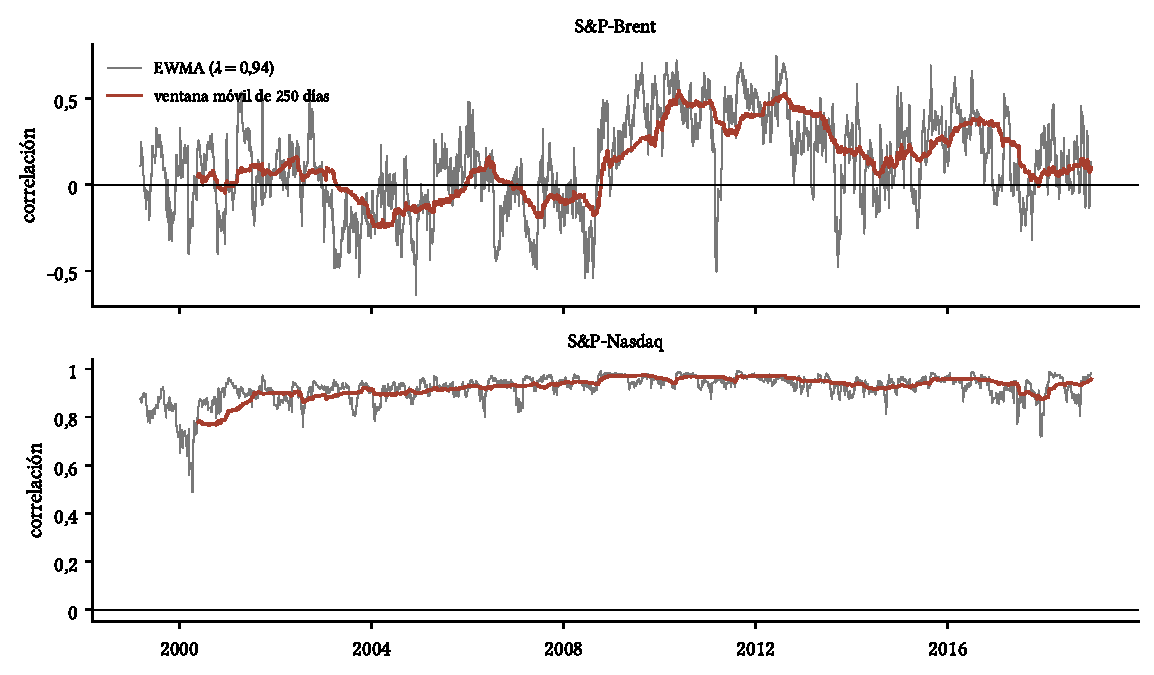
\includegraphics[width=0.92\linewidth]{graficos/cap12_ej01_correlaciones.pdf}
\caption{Correlación diaria S\&P--Brent y S\&P--Nasdaq con EWMA y con ventana móvil de 250 días.}
\label{fig:corrmov}
\end{figure}

\begin{conclusion}
Una sola correlación para veinte años oculta dos regímenes muy distintos. La EWMA y la ventana móvil detectan los
cambios, pero la primera es muy ruidosa y la segunda reacciona con retraso; el DCC busca un punto intermedio
estimado con los datos.
\end{conclusion}
\end{ejresuelto}

\begin{ejresuelto}{DCC para el S\&P 500 y el Brent}\label{ej:dcc2}
\enunciado Estime un DCC(1,1) en dos etapas para el S\&P 500 y el Brent, compárelo con el CCC y describa la
evolución de la correlación.

\solucion
\paso{Paso 1. Primera etapa.} GARCH(1,1) normales: para el S\&P 500, $\hat\alpha=0{,}1024$ y $\hat\beta=0{,}8865$;
para el Brent, $\hat\alpha=0{,}0468$ y $\hat\beta=0{,}9524$ (en esta muestra, que termina en 2018).

\paso{Paso 2. Segunda etapa.}
\begin{align*}
  \hat a &= 0{,}0130\quad(0{,}0027),\\
  \hat b &= 0{,}9844\quad(0{,}0035),\\
  \hat a+\hat b &= 0{,}9974 .
\end{align*}
La correlación es muy persistente: la vida media de una desviación respecto de su nivel de largo plazo es
$\ln0{,}5/\ln0{,}9974=266$ días. El valor de $\ell_C$ es $115{,}97$ con el DCC y $40{,}19$ con el CCC
($\hat\rho=0{,}131$), así que
\begin{align*}
  LR &= 2\,(115{,}97-40{,}19)\\
     &= 151{,}56,
\end{align*}
enorme frente a cualquier valor crítico razonable: la correlación no es constante.

\paso{Paso 3. Evolución.} La correlación DCC promedio fue $-0{,}12$ en 2003, $-0{,}06$ en 2008, $0{,}30$ en 2009 y
$0{,}39$ en 2012, para bajar a $0{,}13$ en 2018. Su mínimo, $-0{,}27$, ocurrió en agosto de 2008, cuando el petróleo
caía desde su máximo histórico mientras las acciones resistían; su máximo, $0{,}52$, en mayo de 2010
(Figura~\ref{fig:dcc2}). Una interpretación habitual es que antes de 2008 los movimientos del petróleo eran sobre
todo choques de oferta (malos para las acciones), mientras que después predominaron los choques de demanda
global, que mueven a ambos en la misma dirección.

\codigoweb{cap12_ej02}
\salidaR{cap12_ej02_R.txt}
\lectura{cap12_ej02}

\RvsPy Ni R base ni \texttt{statsmodels} o \texttt{arch} incluyen el DCC, de modo que la verificación es entre
nuestras dos implementaciones, que coinciden en todas las cifras. En Python, la forma cuadrática
$\mathbf z_t'R_t^{-1}\mathbf z_t$ para todos los $t$ a la vez se calcula con \texttt{np.linalg.solve} sobre el
arreglo tridimensional y \texttt{np.einsum}; en R, con un \texttt{sapply} sobre $t$. La restricción $a+b<1$ se
impone devolviendo un valor enorme de la función objetivo cuando se viola.

\begin{figure}[ht]
\centering
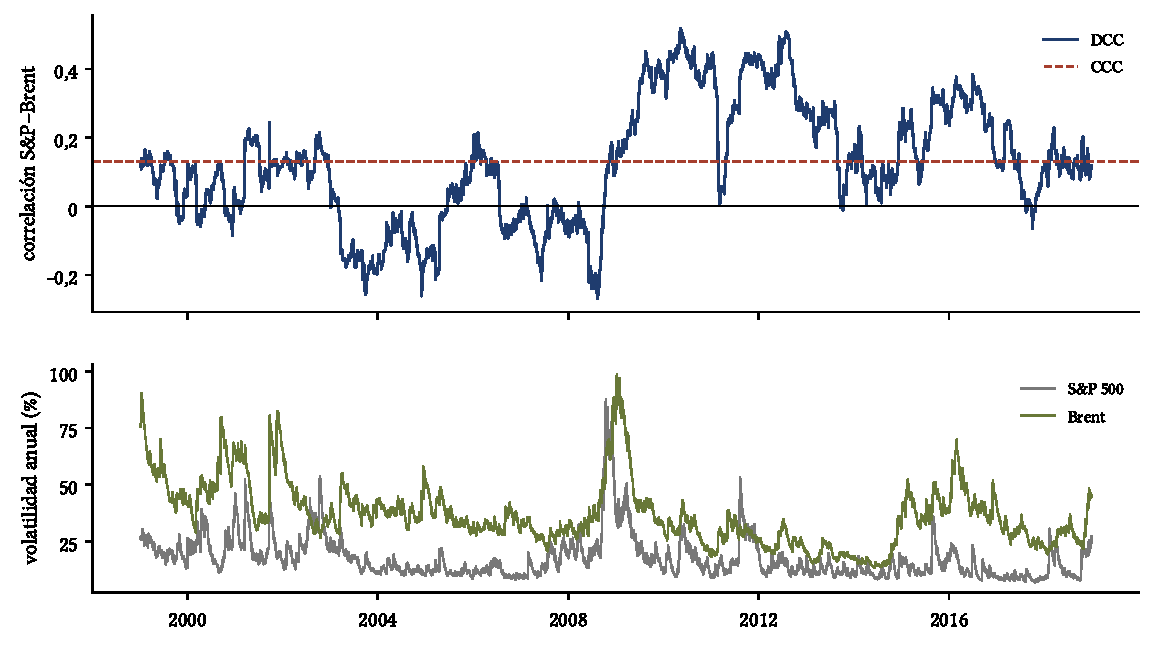
\includegraphics[width=0.92\linewidth]{graficos/cap12_ej02_dcc.pdf}
\caption{Arriba: correlación condicional DCC entre el S\&P 500 y el Brent, y la correlación constante del CCC.
Abajo: volatilidades condicionales anualizadas de la primera etapa.}
\label{fig:dcc2}
\end{figure}

\begin{conclusion}
La correlación entre el petróleo y las acciones de EE.\,UU.\ cambió de signo alrededor de 2008 y es muy
persistente. Un modelo de correlación constante habría subestimado el riesgo conjunto después de 2009.
\end{conclusion}
\end{ejresuelto}

\begin{ejresuelto}{DCC trivariado y la crisis de 2008}\label{ej:dcc3}
\enunciado Estime un DCC con las tres series y compare las correlaciones promedio en calma (enero de 2006 a
agosto de 2008), en la crisis (septiembre de 2008 a marzo de 2009) y en 2017--2018.

\solucion
\paso{Paso 1. Estimación.} $\hat a=0{,}0225$ (0,0029) y $\hat b=0{,}9732$ (0,0040); el estadístico $LR$ frente al
CCC es 788,73. El menor autovalor de las 4\,615 matrices $R_t$ es $0{,}0295$, positivo como garantiza la
Proposición~\ref{prop:dccpd}.

\paso{Paso 2. Correlaciones por período.}
\begin{center}\small
\begin{tabular}{@{}lrrr@{}}
\toprule
Período & S\&P--Nasdaq & S\&P--Brent & Nasdaq--Brent \\
\midrule
Calma 2006--2008  & 0,933 & $-0{,}053$ & $-0{,}066$ \\
Crisis 2008--2009 & 0,961 & 0,161 & 0,141 \\
2017--2018        & 0,910 & 0,103 & 0,035 \\
\bottomrule
\end{tabular}
\end{center}
Todas las correlaciones subieron en la crisis, cuando las volatilidades anuales promediaron 50\,\% en las acciones
y 71\,\% en el petróleo (Figura~\ref{fig:dcc3}).

\paso{Paso 3. Una limitación.} El DCC impone los mismos $a$ y $b$ a todos los pares. Las estimaciones cambian
al agregar el Nasdaq ($\hat a+\hat b=0{,}9957$ frente a $0{,}9974$): el modelo busca un compromiso entre la
correlación S\&P--Nasdaq, alta y estable, y la del petróleo, que cambia mucho. Hay extensiones con parámetros
por par o por grupo, a costa de más parámetros.

\codigoweb{cap12_ej03}
\salidaR{cap12_ej03_R.txt}
\lectura{cap12_ej03}

\RvsPy Para verificar que todas las $R_t$ son definidas positivas, Python calcula de una vez los autovalores
de todo el arreglo con \texttt{np.linalg.eigvalsh}. R usa \texttt{eigen} con las opciones \texttt{symmetric = TRUE} y
\texttt{only.values = TRUE} dentro de un \texttt{sapply}.

\begin{figure}[ht]
\centering
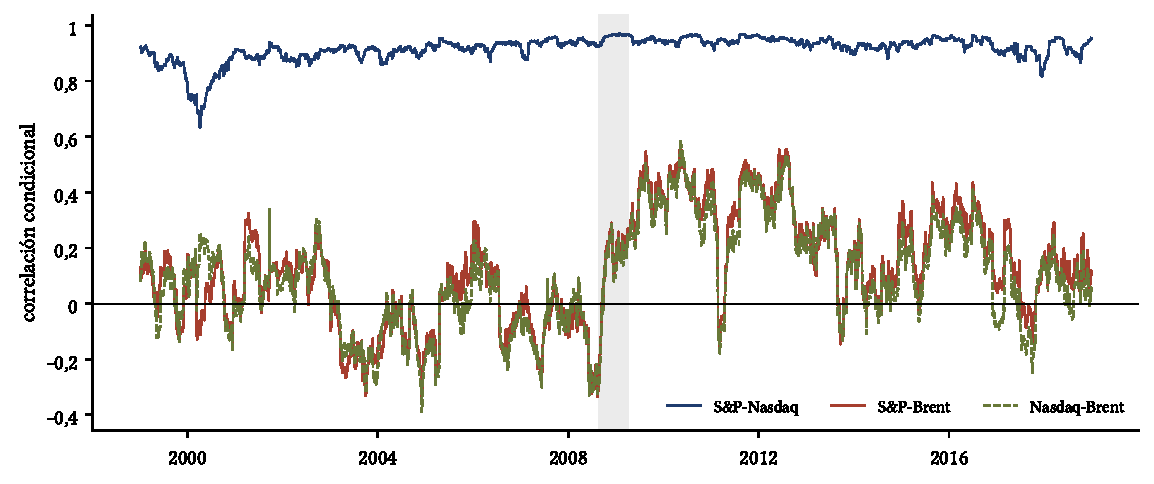
\includegraphics[width=0.92\linewidth]{graficos/cap12_ej03_dcc3.pdf}
\caption{Correlaciones condicionales del DCC trivariado. La franja gris marca la crisis de septiembre de 2008 a
marzo de 2009.}
\label{fig:dcc3}
\end{figure}

\begin{conclusion}
En la crisis de 2008 todas las correlaciones subieron a la vez. El Ejercicio~\ref{ej:contagio} pregunta si fue
contagio o un efecto mecánico de la mayor volatilidad.
\end{conclusion}
\end{ejresuelto}

\begin{ejresuelto}{Cartera de mínima varianza fuera de muestra}\label{ej:minvar}
\enunciado Con datos hasta 2009 estime los GARCH y el DCC de las tres series. Luego, con los parámetros fijos,
construya cada día de 2010--2018 la cartera de mínima varianza usando (i) la covarianza muestral constante de
1999--2009, (ii) la EWMA y (iii) el DCC-GARCH. Compare con la cartera de pesos iguales.

\solucion
\paso{Paso 1. Resultados.} Con 2\,248 días de evaluación ($\hat a=0{,}0189$ y $\hat b=0{,}9796$ en la muestra de
estimación):
\begin{center}\small
\begin{tabular}{@{}lrrrrr@{}}
\toprule
Estrategia & Volatilidad anual & Peso S\&P & Peso Nasdaq & Peso Brent & Rotación diaria \\
\midrule
Constante      & 14,56\,\% & 1,146 & $-0{,}336$ & 0,191 & 0,000 \\
EWMA           & 13,98\,\% & 1,396 & $-0{,}535$ & 0,138 & 0,206 \\
DCC            & 13,81\,\% & 1,407 & $-0{,}507$ & 0,100 & 0,128 \\
Pesos iguales  & 16,37\,\% & 0,333 & 0,333 & 0,333 & 0,000 \\
\bottomrule
\end{tabular}
\end{center}
La cartera DCC es la menos volátil. Las carteras de mínima varianza venden Nasdaq en corto para cubrir
parcialmente la exposición al S\&P 500, aprovechando su altísima correlación.

\paso{Paso 2. ¿Es significativa la diferencia?} Con la prueba de Diebold-Mariano sobre los cuadrados de los
rendimientos de cada cartera: frente a la covarianza constante, $t=4{,}33$; frente a la EWMA, $t=1{,}69$
($p=0{,}09$); frente a los pesos iguales, $t=9{,}02$. El DCC reduce significativamente el riesgo respecto de la
covarianza constante y del reparto ingenuo; su ventaja sobre la EWMA es más modesta, y además rota la cartera un
38\,\% menos ($0{,}128$ frente a $0{,}206$ de suma de cambios absolutos en los pesos por día), lo que reduce costos
de transacción.

\codigoweb{cap12_ej04}
\salidaR{cap12_ej04_R.txt}
\lectura{cap12_ej04}

\RvsPy Para no usar información futura, los GARCH y el DCC se estiman solo con 1999--2009, y después las
recursiones corren sobre toda la muestra con esos parámetros y con la $\bar Q$ de la muestra de estimación (de ahí
el argumento opcional \texttt{Qb} de \texttt{dcc\_filtro}). Los pesos usan $H_t$, que solo depende de datos hasta
$t-1$. En Python, la función de pesos se escribe en una línea con el operador \texttt{:=}.

\begin{figure}[ht]
\centering
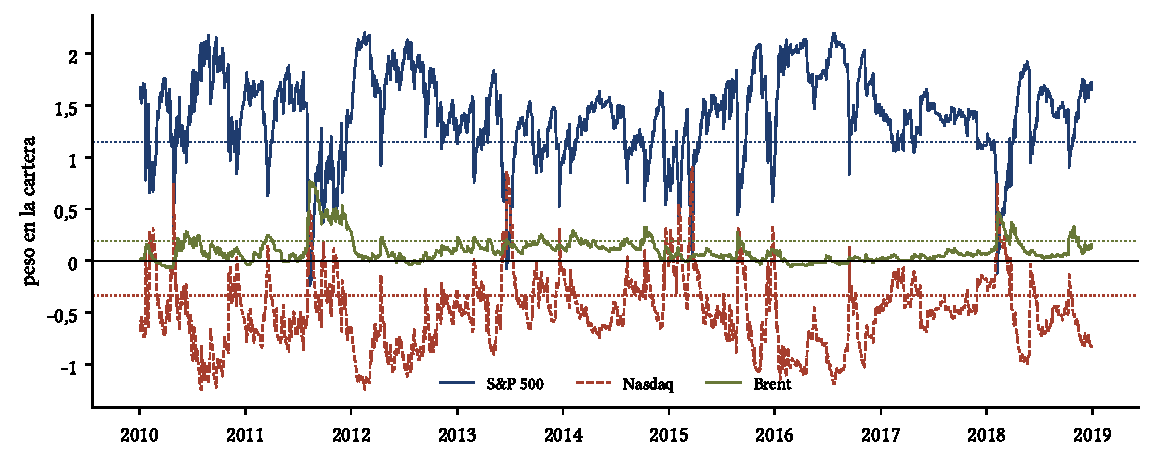
\includegraphics[width=0.92\linewidth]{graficos/cap12_ej04_pesos.pdf}
\caption{Pesos de la cartera de mínima varianza DCC en 2010--2018. Las líneas punteadas son los pesos constantes
calculados con la covarianza muestral de 1999--2009.}
\label{fig:minvar}
\end{figure}

\begin{conclusion}
Modelar la dinámica de las covarianzas tiene valor económico: la cartera DCC es un 5\,\% menos volátil que la de
covarianza constante y un 16\,\% menos que la de pesos iguales, con una rotación moderada.
\end{conclusion}
\end{ejresuelto}

\begin{ejresuelto}{¿Hubo contagio en 2008?}\label{ej:contagio}
\enunciado Compare la correlación del S\&P 500 con el Nasdaq y con el Brent en calma (enero de 2006 a agosto de
2008) y en crisis (septiembre de 2008 a marzo de 2009), antes y después de la corrección de Forbes y Rigobon,
tomando al S\&P 500 como mercado de origen. Use la transformación $z$ de Fisher para contrastar si la correlación
aumentó.

\solucion
\paso{Paso 1. El aumento de volatilidad.} La varianza diaria del S\&P 500 pasó de $1{,}0311$ a $12{,}3838$:
\begin{align*}
  \delta &= \frac{12{,}3838}{1{,}0311}-1\\
         &= 11{,}01 .
\end{align*}
La varianza se multiplicó por doce.

\paso{Paso 2. Brent.} La correlación pasó de $-0{,}113$ a $0{,}224$. Corregida:
\begin{align*}
  \rho^* &= \frac{0{,}2236}{\sqrt{1+11{,}01\,(1-0{,}2236^2)}}\\
         &= \frac{0{,}2236}{\sqrt{11{,}459}}\\
         &= \frac{0{,}2236}{3{,}385}\\
         &= 0{,}066 .
\end{align*}
Con 637 días de calma y 146 de crisis, el error estándar de la diferencia de las transformadas de Fisher es
$\sqrt{1/143+1/634}=0{,}0926$, y
\begin{align*}
  z &= \frac{\operatorname{atanh}(0{,}0661)-\operatorname{atanh}(-0{,}1131)}{0{,}0926}\\
    &= \frac{0{,}0662+0{,}1136}{0{,}0926}\\
    &= 1{,}94 .
\end{align*}
Sin la corrección, $z=3{,}68$. La corrección reduce a la mitad la evidencia de un cambio en la relación entre el
petróleo y las acciones, que queda en el límite de la significancia (valor $p$ unilateral de 0,026, bilateral de
0,052; Figura~\ref{fig:contagio}).

\paso{Paso 3. Nasdaq.} La correlación pasó de $0{,}933$ a $0{,}977$ ($z=5{,}90$), pero la corrección la reduce a
$0{,}798$ ($z=-6{,}36$), es decir, implicaría una \emph{caída} significativa. El resultado no es creíble: el S\&P 500
y el Nasdaq recibieron el mismo choque de volatilidad a la vez, y el supuesto de la
Proposición~\ref{prop:forbes} (que la varianza del componente propio de $y$ no cambie) es falso. La corrección
de Forbes y Rigobon es útil cuando el choque nace claramente en un mercado y se transmite a otro, no cuando un
factor común golpea a ambos.

\codigoweb{cap12_ej05}
\salidaR{cap12_ej05_R.txt}
\lectura{cap12_ej05}

\RvsPy La transformación de Fisher es \texttt{atanh} en R y \texttt{np.arctanh} en Python.

\begin{figure}[ht]
\centering
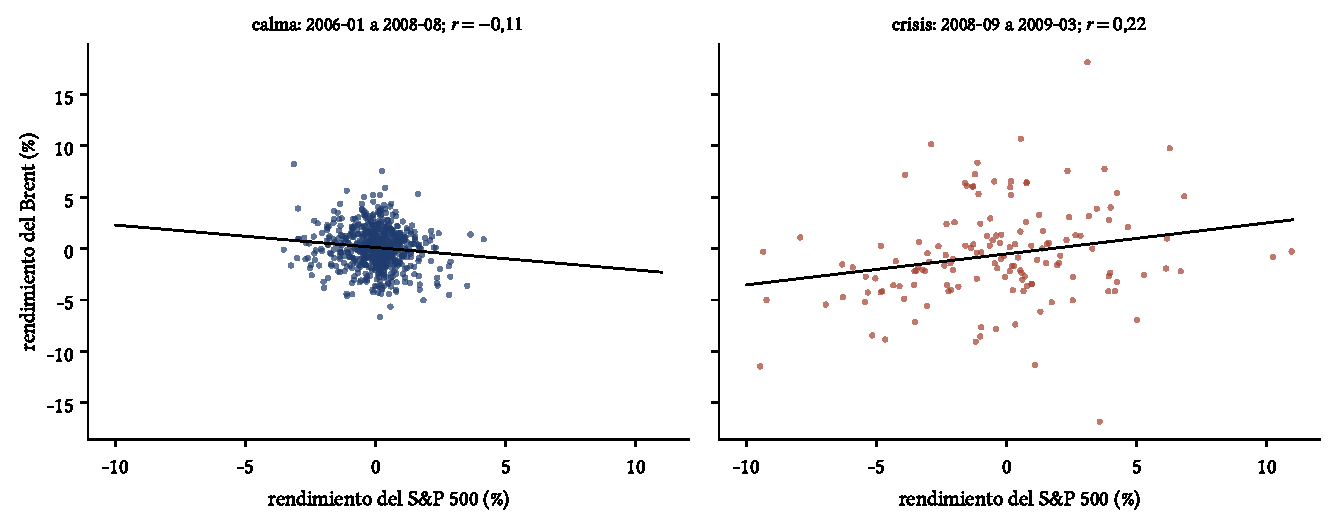
\includegraphics[width=0.92\linewidth]{graficos/cap12_ej05_contagio.pdf}
\caption{Rendimientos diarios del S\&P 500 y del Brent en calma y en crisis, con la recta de MCO. En la crisis el
rango de los rendimientos del S\&P 500 se multiplica, lo que por sí solo eleva la correlación.}
\label{fig:contagio}
\end{figure}

\begin{conclusion}
La correlación entre el petróleo y las acciones aumentó en 2008, pero una buena parte del aumento se explica por
la mayor volatilidad de las acciones. Medir contagio requiere separar el cambio en la relación del cambio en la
escala de los choques.
\end{conclusion}
\end{ejresuelto}

% ---------------------------------------------------------------------
\section{Ejercicios propuestos}
% ---------------------------------------------------------------------

\begin{enumerate}[label=\textbf{\thechapter.\arabic*},leftmargin=*,itemsep=6pt]
  \item Dos activos tienen volatilidades de 20\,\% y 30\,\% y correlación 0,3. Calcule los pesos y la volatilidad de la
  cartera de mínima varianza. \textit{Respuesta: $0{,}766$ y $0{,}234$; 18,67\,\%.}

  \item Con la Proposición~\ref{prop:forbes}, calcule la correlación medida en la crisis si $\rho=0{,}1$ y la
  varianza del mercado de origen se cuadruplica. \textit{Respuesta: $0{,}197$.}

  \item En un DCC con $a=0{,}05$, $b=0{,}93$, $\bar Q$ con unos en la diagonal y $0{,}3$ fuera de ella, y
  $Q_{t-1}=\bar Q$, calcule $\rho_t$ tras los choques $(2,2)$ y $(2,-2)$. \textit{Respuesta: $0{,}422$ y $0{,}074$.}

  \item Demuestre que, si $H_{t-1}$ es definida positiva, la EWMA multivariada produce una $H_t$ definida positiva.

  \item Demuestre que en el CCC la covarianza condicional es $h_{ij,t}=\rho_{ij}\sigma_{it}\sigma_{jt}$ y que la
  razón de cobertura de mínima varianza de $i$ con $j$ es $\rho_{ij}\sigma_{it}/\sigma_{jt}$.

  \item \emph{(Simulación.)} Simule un DCC bivariado con $a=0{,}02$, $b=0{,}97$ y GARCH(1,1) en cada serie, con
  $T=2\,000$. Estime el modelo en dos etapas 200 veces y compare la dispersión de $\hat a$ con su error estándar
  promedio. ¿Son optimistas los errores estándar de la segunda etapa?

  \item \emph{(Con datos de Yahoo Finance y el BCRP.)} Estime un DCC entre el índice S\&P/BVL Perú General, el
  precio del cobre y el tipo de cambio sol/dólar. ¿Sube la correlación entre la bolsa limeña y el cobre en los
  episodios de caída del precio de los metales?

  \item \emph{(Con datos.)} Repita el Ejercicio~\ref{ej:minvar} reestimando los parámetros cada año. ¿Cambia la
  clasificación de los modelos?
\end{enumerate}

% ---------------------------------------------------------------------
\section{Resumen de fórmulas}
% ---------------------------------------------------------------------

\begin{table}[H]
\centering\small
\begin{tabular}{@{}ll@{}}
\toprule
Concepto & Fórmula \\
\midrule
EWMA & $H_t=\lambda H_{t-1}+(1-\lambda)\boldsymbol\varepsilon_{t-1}\boldsymbol\varepsilon_{t-1}'$ \\
CCC & $H_t=D_tRD_t$,\quad $D_t=\operatorname{diag}(\sigma_{it})$ \\
DCC & $Q_t=(1-a-b)\bar Q+a\mathbf z_{t-1}\mathbf z_{t-1}'+bQ_{t-1}$;\quad $R_t=\operatorname{diag}(Q_t)^{-1/2}Q_t\operatorname{diag}(Q_t)^{-1/2}$ \\
Verosimilitud & $\ell_C=-\frac12\sum_t[\ln|R_t|+\mathbf z_t'R_t^{-1}\mathbf z_t-\mathbf z_t'\mathbf z_t]$ \\
Mínima varianza & $\mathbf w^*=H^{-1}\boldsymbol\iota/(\boldsymbol\iota'H^{-1}\boldsymbol\iota)$ \\
Forbes-Rigobon & $\rho^*=\rho_c/\sqrt{1+\delta(1-\rho_c^2)}$ \\
Fisher & $z=[\operatorname{atanh}(\rho_1)-\operatorname{atanh}(\rho_2)]/\sqrt{1/(n_1-3)+1/(n_2-3)}$ \\
\bottomrule
\end{tabular}
\caption{Fórmulas principales del Capítulo 12.}
\end{table}

\section*{Referencias}
\begin{itemize}[leftmargin=*]
  \item Bollerslev, T. (1990). Modelling the coherence in short-run nominal exchange rates: A multivariate
        generalized ARCH model. \emph{Review of Economics and Statistics}, 72(3), 498--505.
  \item Engle, R. F. (2002). Dynamic conditional correlation: A simple class of multivariate generalized
        autoregressive conditional heteroskedasticity models. \emph{Journal of Business \& Economic Statistics},
        20(3), 339--350.
  \item Engle, R. F. y Colacito, R. (2006). Testing and valuing dynamic correlations for asset allocation.
        \emph{Journal of Business \& Economic Statistics}, 24(2), 238--253.
  \item Engle, R. F. y Sheppard, K. (2001). Theoretical and empirical properties of dynamic conditional correlation
        multivariate GARCH. NBER Working Paper 8554.
  \item Forbes, K. J. y Rigobon, R. (2002). No contagion, only interdependence: Measuring stock market
        comovements. \emph{Journal of Finance}, 57(5), 2223--2261.
  \item Longin, F. y Solnik, B. (2001). Extreme correlation of international equity markets. \emph{Journal of
        Finance}, 56(2), 649--676.
\end{itemize}

% =====================================================================
%  Capítulo 13. Valor en riesgo, déficit esperado y valores extremos
% =====================================================================
\part{Riesgo, valoración y temas avanzados}
\chapter[Valor en riesgo y valores extremos]{Valor en riesgo, déficit esperado y teoría de valores extremos}\label{cap:var_riesgo}

\section*{Objetivos de aprendizaje}
Al terminar este capítulo, el lector podrá:
\begin{enumerate}[label=\arabic*.,leftmargin=*]
  \item Definir el valor en riesgo (VaR) y el déficit esperado (ES), calcularlos con modelos normales, $t$ de
        Student, históricos y condicionales, y explicar por qué el VaR no es una medida coherente.
  \item Evaluar un modelo de VaR con las pruebas de Kupiec y Christoffersen y con el semáforo de Basilea.
  \item Modelar la cola de las pérdidas con la distribución de Pareto generalizada y derivar el VaR y el ES
        que implica.
  \item Calcular el riesgo a varios días y reconocer los límites de la regla de la raíz del tiempo.
\end{enumerate}

\section*{Motivación}
Un banco, un fondo de pensiones o una tesorería corporativa necesitan responder una pregunta concreta: ¿cuánto
podemos perder mañana en un mal día? El \emph{valor en riesgo}, popularizado por J.\,P.~Morgan en los noventa y
adoptado por el Comité de Basilea para fijar el capital de los bancos, responde con un cuantil de la distribución
de pérdidas. Pero un cuantil no dice nada sobre lo que ocurre más allá de él, y las crisis financieras ocurren
precisamente allí. Este capítulo reúne lo aprendido sobre colas gruesas (Capítulo~\ref{cap:hechos}) y volatilidad
condicional (Capítulos~\ref{cap:garch} y~\ref{cap:asimetria}) para medir, evaluar y modelar el riesgo extremo.

\paragraph{Datos del capítulo.} Rendimientos logarítmicos diarios del S\&P 500 (1999--2018) y del Brent
(1987--2026). Trabajamos con la pérdida $L_t=-r_t$, en porcentaje: una pérdida positiva es una caída del precio.

% ---------------------------------------------------------------------
\section{Valor en riesgo y déficit esperado}
% ---------------------------------------------------------------------

\begin{definicion}[VaR y ES]
Sea $L$ la pérdida de una posición en un horizonte dado y $p\in(0,1)$ un nivel de confianza (típicamente
$0{,}95$ o $0{,}99$). El \emph{valor en riesgo} es el cuantil $p$ de la pérdida,
\[
  \mathrm{VaR}_p=\inf\{\ell:\ \Pr(L\le\ell)\ge p\},
\]
y el \emph{déficit esperado} (\emph{expected shortfall}) es la pérdida media cuando se supera el VaR:
\[
  \mathrm{ES}_p=\E\bigl[L\mid L\ge\mathrm{VaR}_p\bigr]=\frac{1}{1-p}\int_p^1\mathrm{VaR}_u\,du .
\]
\end{definicion}

Un VaR al 99\,\% de 3\,\% a un día significa que, en promedio, uno de cada cien días la pérdida superará el 3\,\%. El
ES dice cuánto se pierde en promedio en esos días. Desde 2016, las reglas de Basilea para el riesgo de mercado
(\emph{Fundamental Review of the Trading Book}) usan el ES al 97,5\,\% en lugar del VaR al 99\,\%.

\begin{proposicion}[VaR y ES normales]\label{prop:esnormal}
Si $r\sim N(\mu,\sigma^2)$ y $L=-r$, con $z_p=\Phi^{-1}(p)$,
\[
  \mathrm{VaR}_p=-\mu+\sigma z_p,\qquad \mathrm{ES}_p=-\mu+\sigma\,\frac{\phi(z_p)}{1-p}.
\]
\end{proposicion}

\begin{proof}
La pérdida es $L=-\mu+\sigma Z$ con $Z\sim N(0,1)$, que es creciente en $Z$, así que su cuantil $p$ es
$-\mu+\sigma z_p$. Para el ES basta calcular $\E[Z\mid Z\ge z_p]$. Como $\phi'(z)=-z\phi(z)$:
\begin{align*}
  \E[Z\mid Z\ge z_p] &= \frac{1}{\Pr(Z\ge z_p)}\int_{z_p}^{\infty}z\,\phi(z)\,dz\\
                     &= \frac{1}{1-p}\Bigl[-\phi(z)\Bigr]_{z_p}^{\infty}\\
                     &= \frac{1}{1-p}\bigl(0+\phi(z_p)\bigr)\\
                     &= \frac{\phi(z_p)}{1-p}.
\end{align*}
Entonces $\mathrm{ES}_p=-\mu+\sigma\,\E[Z\mid Z\ge z_p]=-\mu+\sigma\phi(z_p)/(1-p)$.
\end{proof}

Con $p=0{,}99$, $z_p=2{,}3263$ y $\phi(z_p)/(1-p)=2{,}6652$: el ES normal es apenas un 15\,\% mayor que el VaR. Con
una $t$ de Student estandarizada de 4 grados de libertad, el VaR al 99\,\% es $2{,}65$ y el ES $3{,}69$, un 39\,\% mayor
(Figura~\ref{fig:vares}). Para la $t$ estandarizada, con $q=t_\nu^{-1}(p)$ y $c=\sqrt{(\nu-2)/\nu}$, un cálculo
similar da
\[
  \mathrm{VaR}_p=-\mu+\sigma\,c\,q,\qquad
  \mathrm{ES}_p=-\mu+\sigma\,c\,\frac{f_\nu(q)}{1-p}\cdot\frac{\nu+q^2}{\nu-1},
\]
donde $f_\nu$ es la densidad de la $t_\nu$.

\begin{figure}[ht]
\centering
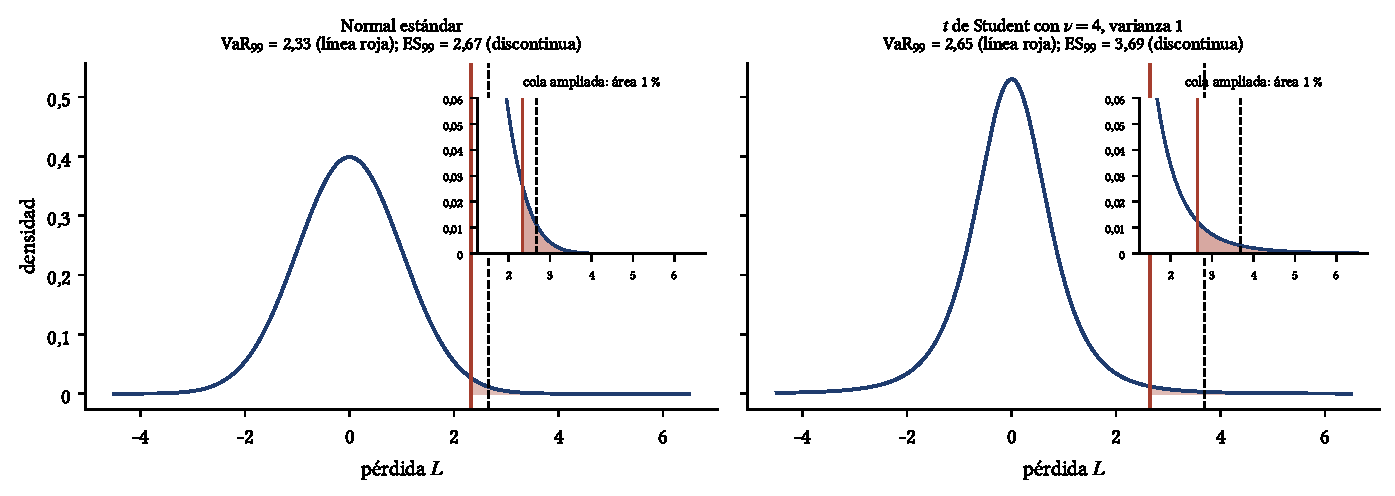
\includegraphics[width=\linewidth]{graficos/cap13_fig_var_es.pdf}
\caption{VaR y ES al 99\,\% para una pérdida normal estándar y para una $t$ de Student con varianza 1. El área
sombreada a la derecha del VaR es el 1\,\%; el ES es su centro de gravedad. Con colas gruesas el VaR sube poco, pero
el ES sube mucho.}
\label{fig:vares}
\end{figure}

\subsection{¿Es el VaR una buena medida de riesgo?}

Artzner, Delbaen, Eber y Heath (1999) propusieron cuatro propiedades que debería cumplir una medida de riesgo
\emph{coherente} $\rho$: monotonía, invarianza ante traslaciones, homogeneidad positiva y
\emph{subaditividad}, $\rho(L_1+L_2)\le\rho(L_1)+\rho(L_2)$, que formaliza que diversificar no aumenta el riesgo.
El ES es coherente; el VaR no siempre es subaditivo.

\begin{ejemplo}[El VaR castiga la diversificación]\label{ej:subaditivo}
Dos bonos independientes pagan 100 o, con probabilidad 4\,\%, nada. Para cada uno, la probabilidad de perder es
$0{,}04<0{,}05$, de modo que $\mathrm{VaR}_{0{,}95}=0$. Para la cartera con ambos,
\begin{align*}
  \Pr(\text{al menos un incumplimiento}) &= 1-0{,}96^2\\
                                         &= 0{,}0784>0{,}05,
\end{align*}
así que el VaR al 95\,\% de la cartera es una pérdida de 100, mayor que $0+0$. Según el VaR, diversificar
\emph{aumentó} el riesgo, porque el VaR ignora el tamaño de las pérdidas más allá del cuantil.
\end{ejemplo}

\subsection{Métodos de estimación}

\begin{itemize}[leftmargin=*]
  \item \textbf{Paramétrico incondicional}: se supone una distribución (normal, $t$) con parámetros constantes.
  \item \textbf{Simulación histórica (HS)}: el VaR es el cuantil empírico de las últimas $n$ pérdidas (por ejemplo,
        $n=500$); el ES, el promedio de las que lo superan. No supone una distribución, pero reacciona tarde a los
        cambios de volatilidad y no puede ir más allá de lo observado.
  \item \textbf{Paramétrico condicional}: $\mathrm{VaR}_{t}=-\mu_t+\sigma_t q_p$, con $\sigma_t$ de un EWMA o un
        GARCH estimado con datos hasta $t-1$.
  \item \textbf{Simulación histórica filtrada (FHS)}: se remuestrean los residuos estandarizados de un GARCH y se
        reescalan con la volatilidad actual (Barone-Adesi y Giannopoulos, 2001). Combina la dinámica del GARCH
        con la forma empírica de las colas.
\end{itemize}

% ---------------------------------------------------------------------
\section{Pruebas retrospectivas}
% ---------------------------------------------------------------------

Sea $I_t=\mathbf 1(L_t>\mathrm{VaR}_t)$ el indicador de una \emph{excepción}. Si el modelo es correcto, los $I_t$
son i.i.d.\ Bernoulli con probabilidad $1-p$ (Christoffersen, 1998): la tasa de excepciones debe ser la correcta
(\emph{cobertura incondicional}) y las excepciones no deben agruparse (\emph{independencia}).

\begin{proposicion}[Prueba de Kupiec]\label{prop:kupiec}
Con $n$ días y $k$ excepciones, sea $q=1-p$ y $\hat\pi=k/n$. El estadístico de razón de verosimilitudes de
$H_0:\Pr(I_t=1)=q$ es
\[
  LR_{uc}=-2\Bigl[(n-k)\ln(1-q)+k\ln q-(n-k)\ln(1-\hat\pi)-k\ln\hat\pi\Bigr]\ \xrightarrow{d}\ \chi^2_1 .
\]
\end{proposicion}

\begin{proof}
Bajo independencia, la verosimilitud de la secuencia de excepciones con probabilidad $\pi$ es
\begin{align*}
  \mathcal L(\pi) &= \prod_{t=1}^{n}\pi^{I_t}(1-\pi)^{1-I_t}\\
                  &= \pi^{k}(1-\pi)^{n-k}.
\end{align*}
Su logaritmo, $\ell(\pi)=k\ln\pi+(n-k)\ln(1-\pi)$, se maximiza en
\begin{align*}
  \ell'(\pi) &= \frac{k}{\pi}-\frac{n-k}{1-\pi}=0,\\
  k(1-\pi)   &= (n-k)\pi,\\
  \hat\pi    &= \frac kn .
\end{align*}
La razón de verosimilitudes es $-2[\ell(q)-\ell(\hat\pi)]$, que es la fórmula del enunciado, con una restricción.
\end{proof}

La prueba de \emph{independencia} de Christoffersen (1998) modela $I_t$ como una cadena de Markov con
probabilidades $\pi_{01}=\Pr(I_t=1\mid I_{t-1}=0)$ y $\pi_{11}=\Pr(I_t=1\mid I_{t-1}=1)$, estimadas con los conteos
de transiciones $n_{ij}$, y contrasta $\pi_{01}=\pi_{11}$:
\[
  LR_{ind}=-2\Bigl[\ell(\hat\pi_1)-\ell(\hat\pi_{01},\hat\pi_{11})\Bigr]\xrightarrow{d}\chi^2_1,
\]
donde $\ell(\hat\pi_1)=(n_{00}+n_{10})\ln(1-\hat\pi_1)+(n_{01}+n_{11})\ln\hat\pi_1$ y
$\ell(\hat\pi_{01},\hat\pi_{11})=n_{00}\ln(1-\hat\pi_{01})+n_{01}\ln\hat\pi_{01}+n_{10}\ln(1-\hat\pi_{11})+n_{11}\ln\hat\pi_{11}$.
La prueba de \emph{cobertura condicional} suma ambas: $LR_{cc}=LR_{uc}+LR_{ind}\sim\chi^2_2$.

\paragraph{El semáforo de Basilea.} Los supervisores bancarios cuentan las excepciones del VaR al 99\,\% en los últimos
250 días. Con 0 a 4 el modelo está en zona \emph{verde}; con 5 a 9, en zona \emph{amarilla}, y el multiplicador del
capital sube de 3 a entre 3,40 y 3,85; con 10 o más, en zona \emph{roja}, y el multiplicador es 4. Las fronteras
salen de la distribución binomial: si el modelo es correcto, $\Pr(X\le4)=0{,}8922$ y $\Pr(X\le9)=0{,}9997$ con
$X\sim\mathrm{Bin}(250;\ 0{,}01)$.

% ---------------------------------------------------------------------
\section{Teoría de valores extremos}
% ---------------------------------------------------------------------

Para el VaR al 99,9\,\% de una cartera, o para una pérdida que ocurre una vez cada diez años, los datos históricos
son escasos y la normal subestima el riesgo. La teoría de valores extremos ofrece un modelo para la cola que no
depende de la distribución completa.

\begin{definicion}[Distribución de Pareto generalizada]
La GPD con parámetro de forma $\xi$ y escala $\beta>0$ tiene función de distribución
\[
  G_{\xi,\beta}(y)=\begin{cases}
     1-\bigl(1+\xi y/\beta\bigr)^{-1/\xi}, & \xi\ne0,\\[2pt]
     1-e^{-y/\beta}, & \xi=0,
  \end{cases}
\]
para $y\ge0$ (y $y\le-\beta/\xi$ si $\xi<0$).
\end{definicion}

El \emph{teorema de Pickands-Balkema-de Haan} dice que, para una clase muy amplia de distribuciones, los excesos
$Y=L-u$ sobre un umbral $u$ alto, condicionados a $L>u$, se distribuyen aproximadamente como una GPD. El índice de
cola $\xi$ determina el tipo: $\xi>0$ para colas gruesas de tipo Pareto (como la $t$, con $\xi=1/\nu$), $\xi=0$ para
colas exponenciales (como la normal) y $\xi<0$ para distribuciones acotadas. La Figura~\ref{fig:gpd} muestra que las
tres formas se distinguen en la cola: en escala logarítmica, la exponencial es una recta, la de $\xi>0$ cae más
despacio y la de $\xi<0$ llega a un máximo finito.

\begin{proposicion}[VaR y ES con la cola GPD]\label{prop:gpdvar}
Sea $u$ un umbral, $n$ el número de observaciones y $N_u$ el de pérdidas mayores que $u$. Si los excesos siguen
una GPD con $0<\xi<1$, para $p>1-N_u/n$:
\begin{align*}
  \mathrm{VaR}_p &= u+\frac{\beta}{\xi}\Bigl[\Bigl(\frac{n}{N_u}(1-p)\Bigr)^{-\xi}-1\Bigr],\\
  \mathrm{ES}_p  &= \frac{\mathrm{VaR}_p}{1-\xi}+\frac{\beta-\xi u}{1-\xi}.
\end{align*}
\end{proposicion}

\begin{proof}
Para $x>u$, la probabilidad de la cola se descompone como
\begin{align*}
  \Pr(L>x) &= \Pr(L>u)\,\Pr(L>x\mid L>u)\\
           &\approx \frac{N_u}{n}\Bigl(1+\xi\,\frac{x-u}{\beta}\Bigr)^{-1/\xi}.
\end{align*}
El VaR resuelve $\Pr(L>x)=1-p$:
\begin{align*}
  \Bigl(1+\xi\,\frac{x-u}{\beta}\Bigr)^{-1/\xi} &= \frac{n}{N_u}(1-p),\\
  1+\xi\,\frac{x-u}{\beta} &= \Bigl(\frac{n}{N_u}(1-p)\Bigr)^{-\xi},\\
  x &= u+\frac\beta\xi\Bigl[\Bigl(\frac{n}{N_u}(1-p)\Bigr)^{-\xi}-1\Bigr].
\end{align*}
Para el ES usamos la \emph{media de los excesos} de la GPD, que es lineal en el umbral: si los excesos sobre $u$ son
GPD$(\xi,\beta)$, los excesos sobre $v>u$ son GPD$(\xi,\beta+\xi(v-u))$, y la media de una GPD es escala$/(1-\xi)$. Así
\begin{align*}
  e(v)=\E[L-v\mid L>v] &= \frac{\beta+\xi(v-u)}{1-\xi}.
\end{align*}
Con $v=\mathrm{VaR}_p$:
\begin{align*}
  \mathrm{ES}_p &= \mathrm{VaR}_p+e(\mathrm{VaR}_p)\\
                &= \mathrm{VaR}_p+\frac{\beta+\xi\,\mathrm{VaR}_p-\xi u}{1-\xi}\\
                &= \frac{(1-\xi)\mathrm{VaR}_p+\xi\,\mathrm{VaR}_p}{1-\xi}+\frac{\beta-\xi u}{1-\xi}\\
                &= \frac{\mathrm{VaR}_p}{1-\xi}+\frac{\beta-\xi u}{1-\xi}. && \qedhere
\end{align*}
\end{proof}

La linealidad de $e(v)$ da una herramienta gráfica para elegir el umbral: el gráfico de la media empírica de los
excesos debe ser aproximadamente una recta con pendiente $\xi/(1-\xi)$ por encima de un buen umbral (Figura~\ref{fig:gpd},
derecha). Elegir $u$ implica un equilibrio: un umbral bajo da muchos excesos pero quizá no GPD (sesgo); uno alto,
pocos excesos (varianza). En la práctica se usa un cuantil entre el 90 y el 97,5\,\% y se verifica la estabilidad
de $\hat\xi$. Los parámetros se estiman por máxima verosimilitud con la log-verosimilitud
\[
  \ell(\xi,\beta)=-N_u\ln\beta-\Bigl(1+\frac1\xi\Bigr)\sum_{i=1}^{N_u}\ln\Bigl(1+\frac{\xi y_i}{\beta}\Bigr).
\]

\begin{figure}[ht]
\centering
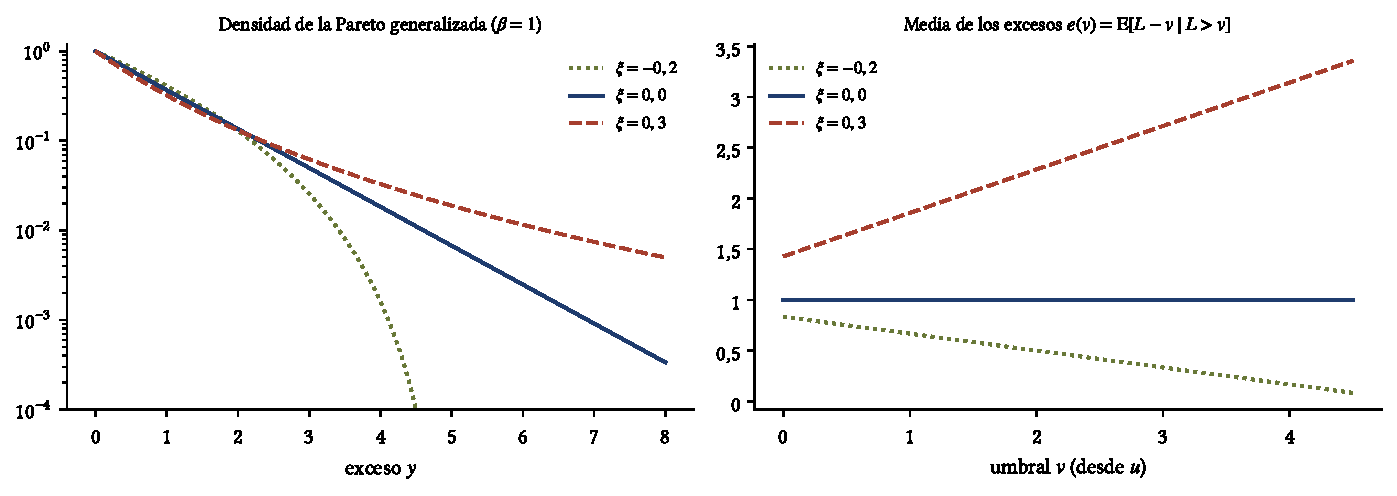
\includegraphics[width=\linewidth]{graficos/cap13_fig_gpd.pdf}
\caption{Izquierda: densidad de la GPD con $\beta=1$ en escala logarítmica. Derecha: su función de media de los
excesos, creciente si $\xi>0$, constante si $\xi=0$ y decreciente si $\xi<0$.}
\label{fig:gpd}
\end{figure}

% ---------------------------------------------------------------------
\section{Riesgo a varios días}
% ---------------------------------------------------------------------

La regulación pide a veces el VaR a 10 días. La \emph{regla de la raíz del tiempo},
$\mathrm{VaR}^{(10)}=\sqrt{10}\,\mathrm{VaR}^{(1)}$, supone que los rendimientos son i.i.d.\ normales con media
cero. Falla por tres razones: la volatilidad revierte a su media (Proposición~\ref{prop:garchpron}), así que la regla
sobreestima el riesgo cuando la volatilidad está alta y lo subestima cuando está baja; la suma de rendimientos con
colas gruesas tiene colas menos gruesas que cada sumando, así que multiplicar el cuantil de un día por $\sqrt{10}$
exagera la cola; y la retroalimentación del GARCH (un día malo eleva la volatilidad de los siguientes) engorda la
cola de las pérdidas acumuladas. La simulación histórica filtrada captura los tres efectos.

% ---------------------------------------------------------------------
\section{Ejercicios resueltos}
% ---------------------------------------------------------------------

\begin{ejresuelto}{VaR y ES incondicionales}\label{ej:varincond}
\enunciado Calcule el VaR y el ES a un día al 95 y al 99\,\% para el S\&P 500 y el Brent con la normal, la $t$ de Student
(con $\nu$ elegido para reproducir la curtosis muestral) y la simulación histórica, y la frecuencia con que cada VaR
fue superado en la muestra.

\solucion
\paso{Paso 1. La $t$ por momentos.} Como la curtosis de la $t_\nu$ es $\kappa=3+6/(\nu-4)$, despejando
\begin{align*}
  \nu &= 4+\frac{6}{\kappa-3}.
\end{align*}
Para el S\&P 500, $\kappa=11{,}17$ y $\nu=4+6/8{,}17=4{,}734$; para el Brent, $\kappa=55{,}97$ y $\nu=4{,}113$.

\paso{Paso 2. VaR normal del S\&P 500 al 99\,\%.} Con $\hat\mu=0{,}0142$ y $\hat\sigma=1{,}2038$:
\begin{align*}
  \mathrm{VaR}_{0{,}99} &= -0{,}0142+1{,}2038\times2{,}3263=2{,}786,\\
  \mathrm{ES}_{0{,}99}  &= -0{,}0142+1{,}2038\times2{,}6652=3{,}194 .
\end{align*}

\paso{Paso 3. Comparación.}
\begin{center}\small
\begin{tabular}{@{}llrrrrrr@{}}
\toprule
 & & \multicolumn{3}{c}{S\&P 500} & \multicolumn{3}{c}{Brent} \\
\cmidrule(lr){3-5}\cmidrule(lr){6-8}
Nivel & Modelo & VaR & ES & Frec. & VaR & ES & Frec. \\
\midrule
95\,\% & normal    & 1,966 & 2,469 & 4,63\,\% & 4,429 & 5,559 & 3,26\,\% \\
       & $t$       & 1,852 & 2,690 & 5,21\,\% & 4,080 & 6,099 & 4,19\,\% \\
       & histórico & 1,882 & 2,910 & 5,01\,\% & 3,799 & 6,133 & 5,00\,\% \\
99\,\% & normal    & 2,786 & 3,194 & 1,83\,\% & 6,271 & 7,188 & 1,32\,\% \\
       & $t$       & 3,138 & 4,203 & 1,27\,\% & 7,134 & 9,873 & 0,99\,\% \\
       & histórico & 3,362 & 4,814 & 1,01\,\% & 7,120 & 11,289 & 1,01\,\% \\
\bottomrule
\end{tabular}
\end{center}
Al 95\,\% los tres modelos se parecen y la normal incluso \emph{sobreestima} el VaR (la cola empieza a engordar más
lejos). Al 99\,\% la normal subestima: su VaR del S\&P 500 se supera el 1,83\,\% de los días, casi el doble de lo
previsto, y su ES es un tercio menor que el histórico. La Figura~\ref{fig:colas} muestra por qué: en escala
logarítmica, la cola normal se hunde mientras la empírica sigue casi recta.

\codigoweb{cap13_ej01}
\salidaR{cap13_ej01_R.txt}
\lectura{cap13_ej01}

\RvsPy El cuantil empírico usa interpolación lineal en ambos lenguajes: \texttt{quantile(..., type = 7)} en R y el
método por omisión de \texttt{np.quantile}. Con otros métodos el VaR histórico cambia en la tercera cifra. En R, los
nombres de lista con tilde (\texttt{"histórico"}) deben ir entre comillas.

\begin{figure}[ht]
\centering
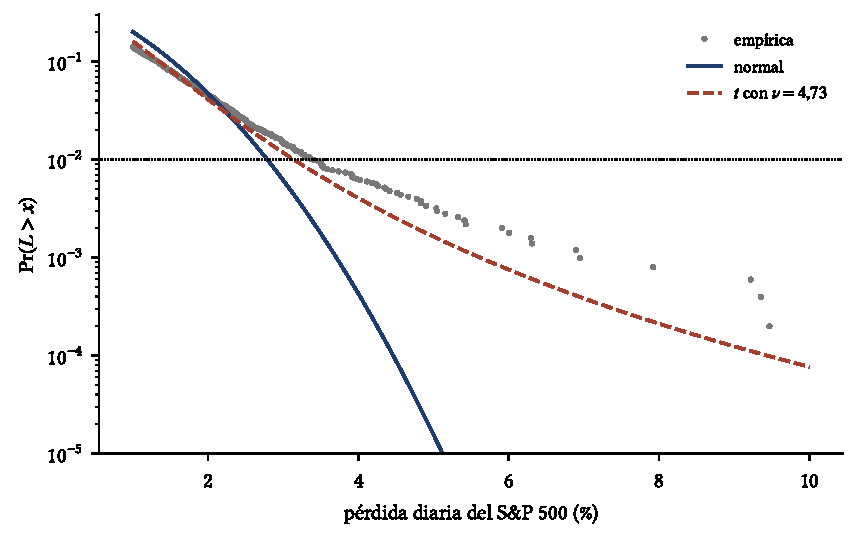
\includegraphics[width=0.7\linewidth]{graficos/cap13_ej01_colas.pdf}
\caption{Probabilidad de que la pérdida diaria del S\&P 500 supere $x$: empírica, normal y $t$ de Student. La línea
horizontal marca el 1\,\%.}
\label{fig:colas}
\end{figure}

\begin{conclusion}
La normal es aceptable al 95\,\%, pero subestima el riesgo al 99\,\% y, sobre todo, el déficit esperado. Para el Brent,
cuya cola es mucho más gruesa, el ES histórico al 99\,\% es un 57\,\% mayor que el normal.
\end{conclusion}
\end{ejresuelto}

\begin{ejresuelto}{Prueba retrospectiva del VaR del S\&P 500}\label{ej:backtest}
\enunciado Calcule cada día de 2001 a 2018 el VaR al 99\,\% a un día del S\&P 500 con: (i) simulación histórica con 500
días; (ii) EWMA normal ($\lambda=0{,}94$, media cero); (iii) GARCH(1,1)-$t$ reestimado cada enero con todos los datos
anteriores. Aplique las pruebas de Kupiec, Christoffersen y de cobertura condicional.

\solucion
\paso{Paso 1. Resultados.} En 4\,527 días se esperan $45{,}3$ excepciones:
\begin{center}\small
\begin{tabular}{@{}lrrrrrr@{}}
\toprule
Modelo & VaR medio & Excepciones & Tasa & $LR_{uc}$ & $LR_{ind}$ & $LR_{cc}$ \\
\midrule
HS-500      & 3,016 & 73 & 1,61\,\% & 14,47 & 10,71 & 25,18 \\
EWMA normal & 2,375 & 96 & 2,12\,\% & 43,44 & 3,25 & 46,69 \\
GARCH-$t$   & 2,585 & 65 & 1,44\,\% & 7,65 & 3,01 & 10,66 \\
\bottomrule
\end{tabular}
\end{center}

\paso{Paso 2. Kupiec para el GARCH-$t$.} Con $\hat\pi=65/4\,527=0{,}01436$:
\begin{align*}
  \ell(0{,}01) &= 4\,462\ln0{,}99+65\ln0{,}01=-344{,}18,\\
  \ell(\hat\pi) &= 4\,462\ln0{,}98564+65\ln0{,}01436=-340{,}35,\\
  LR_{uc} &= -2\,(-344{,}18+340{,}35)=7{,}65,
\end{align*}
con valor $p$ de $0{,}006$: se rechaza la cobertura correcta, aunque el GARCH-$t$ es el mejor de los tres.

\paso{Paso 3. Interpretación.} Los tres modelos tienen más excepciones de las debidas. La EWMA normal es la peor en
cobertura (96): la normal subestima la cola. La simulación histórica tiene el VaR medio más alto, pero aun así
falla 73 veces porque sus excepciones se concentran: 21 en 2008 (de 253 días), cuando la ventana de 500 días todavía
reflejaba la calma de 2006--2007 (Figura~\ref{fig:backtest}). Por eso es la única que rechaza la independencia
($LR_{ind}=10{,}71$, $p=0{,}001$). Los modelos condicionales reaccionan en días: en 2008 la EWMA tuvo 9 excepciones y
el GARCH-$t$, 7.

\codigoweb{cap13_ej02}
\salidaR{cap13_ej02_R.txt}
\lectura{cap13_ej02}

\RvsPy El GARCH-$t$ se reestima 18 veces con la función \texttt{garch\_fit} del Capítulo~\ref{cap:garch}; con los
parámetros de cada año, la recursión corre sobre toda la serie y se toman las varianzas de ese año, que solo
dependen de datos anteriores. Las excepciones coinciden una a una entre R y Python. Las series de VaR se guardan en
un CSV para el ejercicio siguiente; en R hay que pasar \texttt{check.names = FALSE} a \texttt{data.frame} para que
nombres como \texttt{HS-500} no se conviertan en \texttt{HS.500}.

\begin{figure}[ht]
\centering
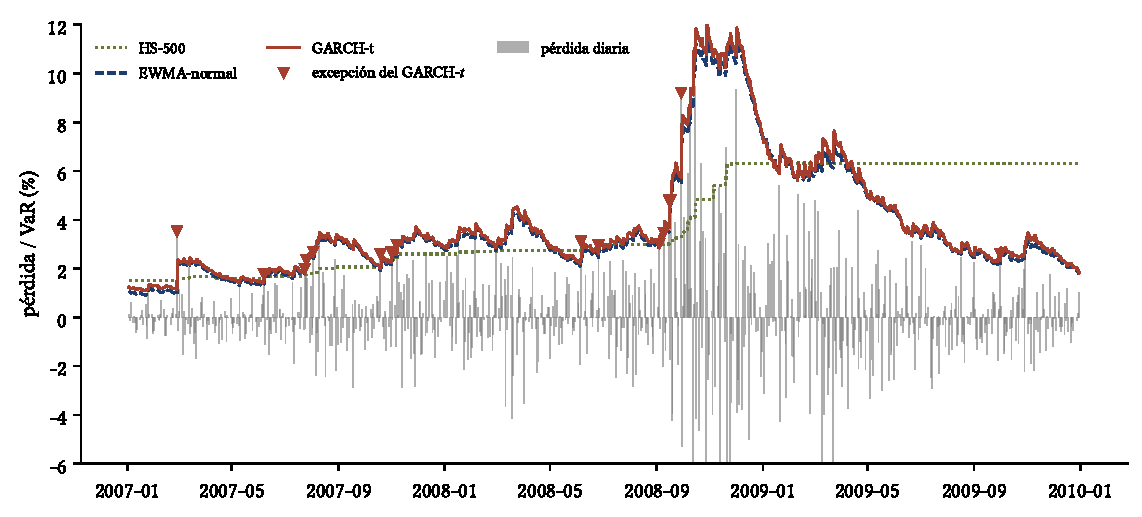
\includegraphics[width=0.92\linewidth]{graficos/cap13_ej02_backtest.pdf}
\caption{Pérdidas diarias del S\&P 500 y VaR al 99\,\% de los tres modelos en 2007--2009. La simulación histórica
(punteada) tarda meses en reaccionar a la crisis; los triángulos son las excepciones del GARCH-$t$.}
\label{fig:backtest}
\end{figure}

\begin{conclusion}
Los modelos condicionales siguen a la volatilidad, y el de colas $t$ es el que más se acerca a la cobertura correcta.
La simulación histórica falla en el peor momento: cuando empieza una crisis.
\end{conclusion}
\end{ejresuelto}

\begin{ejresuelto}{El semáforo de Basilea}\label{ej:semaforo}
\enunciado Con los VaR del Ejercicio~\ref{ej:backtest}, cuente las excepciones de cada año calendario y asigne la zona
del semáforo de Basilea.

\solucion
\paso{Paso 1. Conteos.}
\begin{center}\small
\begin{tabular}{@{}lrrr|lrrr@{}}
\toprule
Año & HS & EWMA & GARCH-$t$ & Año & HS & EWMA & GARCH-$t$ \\
\midrule
2001 & 4 & 4 & 2 & 2010 & 0 & 9 & 6 \\
2002 & 5 & 2 & 2 & 2011 & 5 & 6 & 6 \\
2003 & 1 & 1 & 0 & 2012 & 0 & 5 & 4 \\
2004 & 0 & 3 & 0 & 2013 & 0 & 5 & 3 \\
2005 & 2 & 3 & 0 & 2014 & 2 & 10 & 6 \\
2006 & 4 & 5 & 3 & 2015 & 6 & 6 & 4 \\
2007 & 11 & 12 & 8 & 2016 & 3 & 2 & 2 \\
2008 & 21 & 9 & 7 & 2017 & 0 & 4 & 3 \\
2009 & 0 & 2 & 1 & 2018 & 9 & 8 & 8 \\
\bottomrule
\end{tabular}
\end{center}

\paso{Paso 2. Zonas.} La simulación histórica pasa 12 años en verde, 4 en amarillo y 2 en rojo (2007 y 2008); la EWMA,
8, 8 y 2 (2007 y 2014); el GARCH-$t$, 12, 6 y ninguno en rojo. Con los recargos de Basilea, el multiplicador medio del
capital sería 3,231 para la simulación histórica, 3,369 para la EWMA y 3,203 para el GARCH-$t$.

\paso{Paso 3. Paradoja de la simulación histórica.} Fuera de las crisis, la simulación histórica casi nunca falla
(siete años con 0 o 1 excepción): su VaR es demasiado \emph{conservador} en la calma y demasiado \emph{laxo} al
inicio de una crisis. Un banco que la usara inmovilizaría capital de más casi siempre y caería en la zona roja cuando
más duele (Figura~\ref{fig:semaforo}).

\codigoweb{cap13_ej03}
\salidaR{cap13_ej03_R.txt}
\lectura{cap13_ej03}

\RvsPy Cada lenguaje lee el CSV que generó en el ejercicio anterior. Los recargos (0,40; 0,50; 0,65; 0,75 y 0,85 para 5 a 9
excepciones) se guardan en un vector indexado por el número de excepciones; en R los índices empiezan en 1, por eso
se usa \texttt{extra[k + 1]}.

\begin{figure}[ht]
\centering
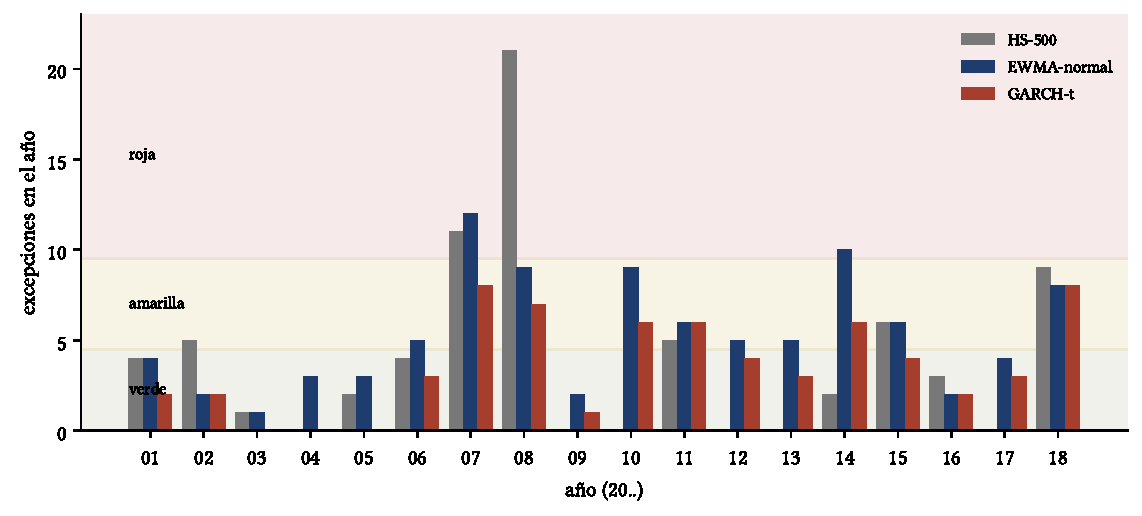
\includegraphics[width=0.92\linewidth]{graficos/cap13_ej03_semaforo.pdf}
\caption{Excepciones anuales del VaR al 99\,\% del S\&P 500 y zonas del semáforo de Basilea.}
\label{fig:semaforo}
\end{figure}

\begin{conclusion}
El GARCH-$t$ nunca habría llevado al banco a la zona roja en 18 años; la simulación histórica y la EWMA, dos veces
cada una. La prueba de Basilea es exigente con los modelos que no reaccionan a la volatilidad.
\end{conclusion}
\end{ejresuelto}

\begin{ejresuelto}{Valores extremos del Brent y del S\&P 500}\label{ej:evt}
\enunciado Estime una GPD para los excesos de las pérdidas diarias sobre los cuantiles 90, 95 y 97,5\,\%. Con el umbral del
95\,\%, calcule el VaR y el ES al 99; 99,5 y 99,9\,\% y compárelos con la normal, la $t$ y la simulación histórica.

\solucion
\paso{Paso 1. Estabilidad de $\hat\xi$.}
\begin{center}\small
\begin{tabular}{@{}lrrrr@{}}
\toprule
 & \multicolumn{2}{c}{Brent} & \multicolumn{2}{c}{S\&P 500} \\
\cmidrule(lr){2-3}\cmidrule(lr){4-5}
Umbral & $\hat\xi$ (ee) & $N_u$ & $\hat\xi$ (ee) & $N_u$ \\
\midrule
90\,\%   & 0,270 (0,039) & 912 & 0,155 (0,050) & 503 \\
95\,\%   & 0,371 (0,063) & 456 & 0,168 (0,072) & 252 \\
97,5\,\% & 0,445 (0,101) & 228 & 0,236 (0,121) & 126 \\
\bottomrule
\end{tabular}
\end{center}
La cola del Brent es mucho más gruesa ($\hat\xi\approx0{,}37$, equivalente a una $t$ con menos de 3 grados de
libertad) que la del S\&P 500 ($\hat\xi\approx0{,}17$). En el Brent $\hat\xi$ crece con el umbral: la cola extrema
está dominada por unos pocos días (abril de 2020, 1991, 2026).

\paso{Paso 2. VaR con la GPD.} Para el Brent, $u=3{,}799$, $N_u=456$, $n=9\,121$, $\hat\xi=0{,}3706$ y
$\hat\beta=1{,}4650$. Al 99\,\%:
\begin{align*}
  \frac{n}{N_u}(1-p) &= 20{,}002\times0{,}01=0{,}20002,\\
  0{,}20002^{-0{,}3706} &= 1{,}8156,\\
  \mathrm{VaR}_{0{,}99} &= 3{,}799+\frac{1{,}4650}{0{,}3706}\,(1{,}8156-1)=7{,}023,\\
  \mathrm{ES}_{0{,}99} &= \frac{7{,}023}{0{,}6294}+\frac{1{,}4650-0{,}3706\times3{,}799}{0{,}6294}=11{,}16+0{,}09=11{,}25 .
\end{align*}

\paso{Paso 3. Comparación (Brent).}
\begin{center}\small
\begin{tabular}{@{}lrrrrrrrr@{}}
\toprule
 & \multicolumn{2}{c}{GPD} & \multicolumn{2}{c}{Normal} & \multicolumn{2}{c}{$t$} & \multicolumn{2}{c}{Histórico} \\
\cmidrule(lr){2-3}\cmidrule(lr){4-5}\cmidrule(lr){6-7}\cmidrule(lr){8-9}
Nivel & VaR & ES & VaR & ES & VaR & ES & VaR & ES \\
\midrule
99\,\%   & 7,02 & 11,25 & 6,27 & 7,19 & 7,13 & 9,87 & 7,12 & 11,29 \\
99,5\,\% & 9,13 & 14,59 & 6,95 & 7,80 & 8,74 & 11,92 & 9,02 & 14,73 \\
99,9\,\% & 16,69 & 26,61 & 8,34 & 9,09 & 13,50 & 18,09 & 16,82 & 26,70 \\
\bottomrule
\end{tabular}
\end{center}
La GPD reproduce casi exactamente los cuantiles y ES empíricos incluso al 99,9\,\%, donde hay solo 9 observaciones. La
normal da un VaR al 99,9\,\% de la mitad del real, y un ES de un tercio. La $t$ por momentos mejora, pero se queda corta
porque su $\nu$ se calibró con la curtosis, que mide toda la distribución y no solo la cola (Figura~\ref{fig:evt}).

\codigoweb{cap13_ej04}
\salidaR{cap13_ej04_R.txt}
\lectura{cap13_ej04}

\RvsPy La verosimilitud de la GPD se maximiza con Nelder-Mead en ambos lenguajes; R y Python coinciden hasta la
sexta decimal, y \texttt{genpareto.fit(y, floc=0)} de \texttt{scipy} da el mismo $\hat\xi=0{,}3705$. Ojo con la
parametrización: en \texttt{scipy} el parámetro de forma se llama \texttt{c} y coincide con $\xi$.

\begin{figure}[ht]
\centering
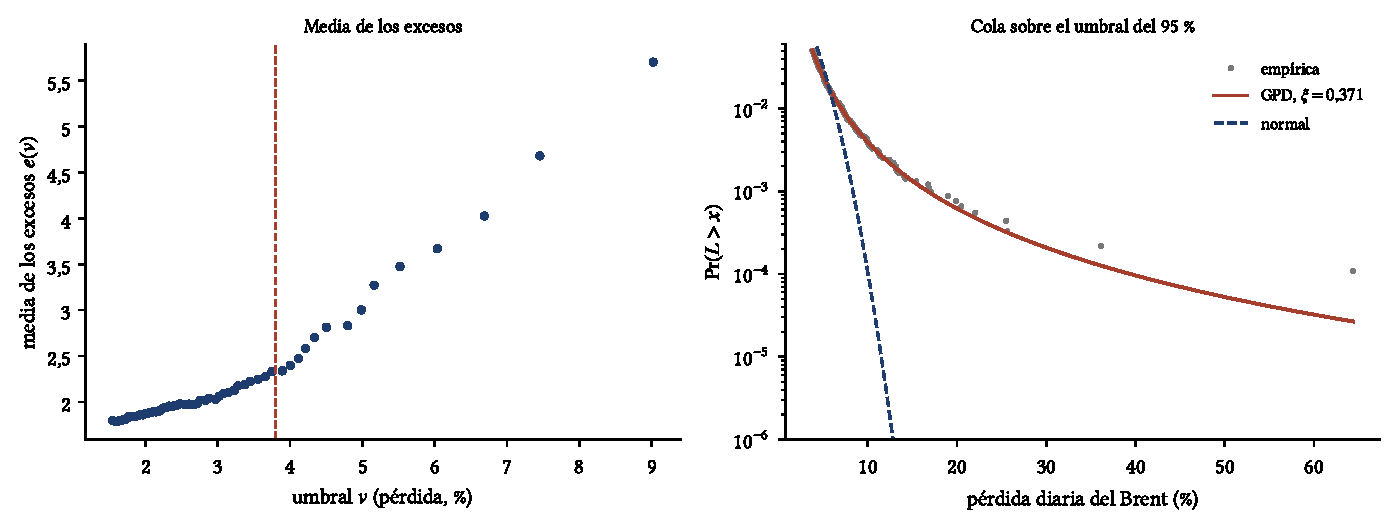
\includegraphics[width=\linewidth]{graficos/cap13_ej04_evt.pdf}
\caption{Brent. Izquierda: media empírica de los excesos; por encima del umbral del 95\,\% (línea discontinua) crece
aproximadamente en línea recta. Derecha: probabilidad empírica de la cola frente a la GPD ajustada y a la normal.}
\label{fig:evt}
\end{figure}

\begin{conclusion}
La teoría de valores extremos permite estimar cuantiles muy altos con un modelo apoyado en la teoría, y no solo en
unos pocos datos. Para el petróleo, la diferencia entre la normal y la GPD al 99,9\,\% es de más de 8 puntos
porcentuales de pérdida diaria.
\end{conclusion}
\end{ejresuelto}

\begin{ejresuelto}{VaR a 10 días del Brent}\label{ej:var10}
\enunciado Con un GARCH(1,1)-$t$ estimado para el Brent, calcule el VaR al 99\,\% a 10 días el 31 de diciembre de 2019 (calma)
y el 3 de noviembre de 2026 (alta volatilidad) con: (i) la regla de la raíz aplicada al VaR $t$ a un día; (ii) la
varianza acumulada del GARCH con un cuantil normal; (iii) simulación histórica filtrada con 100\,000 trayectorias.

\solucion
\paso{Paso 1. Varianza acumulada.} Por el Corolario~\ref{cor:varH}, con $\hat\phi=0{,}9955$ y la varianza de largo
plazo de $13{,}29$: el 31 de diciembre de 2019 la varianza de mañana era $1{,}519^2=2{,}31$, muy por debajo, y la
desviación estándar acumulada a 10 días es $5{,}03$\,\%, algo más que $\sqrt{10}\times1{,}519=4{,}80$\,\%. El 3 de noviembre
de 2026 era $4{,}762^2=22{,}68$, por encima, y la acumulada es $15{,}00$\,\%, algo menos que $\sqrt{10}\times4{,}762=15{,}06$\,\%.

\paso{Paso 2. Resultados.}
\begin{center}\small
\begin{tabular}{@{}lrr@{}}
\toprule
VaR al 99\,\% a 10 días & 2019-12-31 & 2026-11-03 \\
\midrule
VaR $t$ a 1 día & 3,89 & 12,31 \\
Raíz del tiempo: $\sqrt{10}\times$VaR & 12,31 & 38,94 \\
Varianza GARCH acumulada, cuantil normal & 11,17 & 34,37 \\
Simulación filtrada (R) & 12,64 & 39,58 \\
Simulación filtrada (Python) & 12,97 & 39,07 \\
\bottomrule
\end{tabular}
\end{center}
El enfoque de la varianza acumulada con un cuantil normal es el más bajo: corrige la reversión a la media pero ignora
que la pérdida a 10 días sigue teniendo colas gruesas. La simulación filtrada da cifras parecidas a la regla de la raíz,
pero por razones distintas: la regla exagera la cola (multiplica un cuantil $t$ de un día) y la simulación la
reconstruye con la retroalimentación del GARCH, en la que un día malo eleva la volatilidad de los siguientes. El ES
simulado es de alrededor de 16\,\% en 2019 y de 49 a 50\,\% en 2026 (Figura~\ref{fig:var10}).

\codigoweb{cap13_ej05}
\salidaR{cap13_ej05_R.txt}
\lectura{cap13_ej05}

\RvsPy Los métodos analíticos coinciden en todas las cifras. La simulación difiere entre R y Python en torno al 2--3\,\%
porque cada lenguaje usa su propio generador de números aleatorios; la diferencia es grande para 100\,000
trayectorias porque la cola de la pérdida acumulada la dominan unos pocos residuos estandarizados extremos (como el
de abril de 2020), que se sortean con probabilidad $1/9\,121$ en cada día. Python vectoriza las trayectorias y R
recorre un bucle; con 100\,000 trayectorias, R tarda unos 15 segundos.

\begin{figure}[ht]
\centering
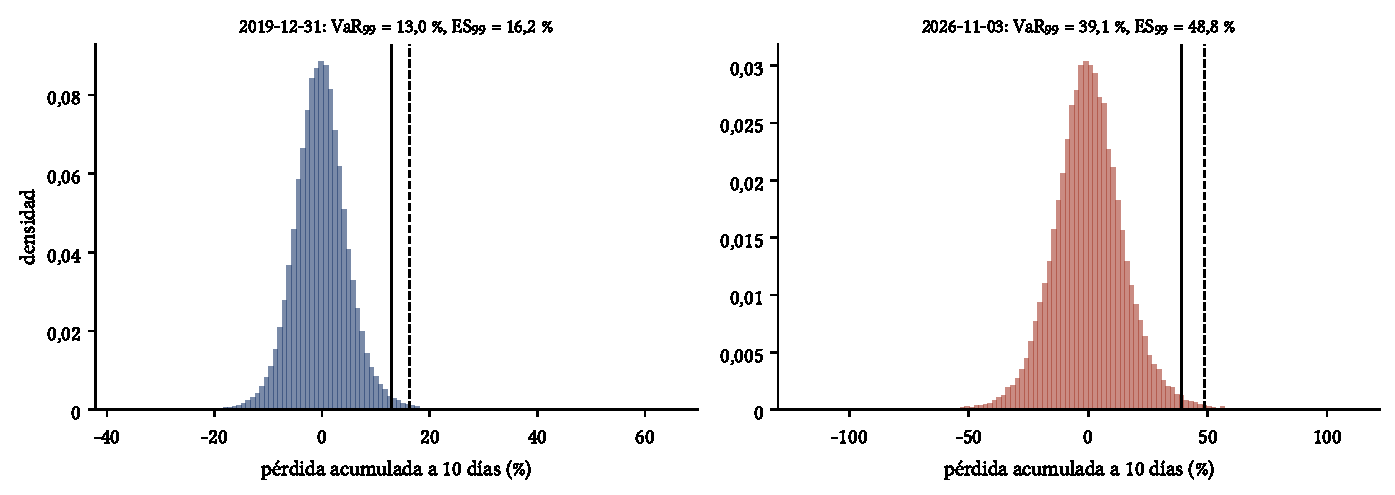
\includegraphics[width=\linewidth]{graficos/cap13_ej05_10dias.pdf}
\caption{Distribución simulada de la pérdida acumulada a 10 días del Brent, en calma y en alta volatilidad, con el VaR
(línea continua) y el ES (discontinua) al 99\,\%.}
\label{fig:var10}
\end{figure}

\begin{conclusion}
El riesgo a varios días depende del nivel de volatilidad de partida y de la forma de la cola, y la regla de la raíz
acierta en este caso por casualidad, al compensarse dos errores. La simulación filtrada es el método más completo,
pero su precisión en la cola extrema requiere muchas trayectorias.
\end{conclusion}
\end{ejresuelto}

% ---------------------------------------------------------------------
\section{Ejercicios propuestos}
% ---------------------------------------------------------------------

\begin{enumerate}[label=\textbf{\thechapter.\arabic*},leftmargin=*,itemsep=6pt]
  \item Un portafolio de 10 millones de soles tiene rendimiento diario normal con media 0 y desviación 1,5\,\%. Calcule el VaR
  y el ES al 99\,\% a un día y a 10 días (regla de la raíz). \textit{Respuesta: 349\,000 y 400\,000 soles; 1\,103\,000 y 1\,264\,000.}

  \item Demuestre que, para una $t_\nu$, $\E[X\mid X>q]=\frac{f_\nu(q)}{1-F_\nu(q)}\cdot\frac{\nu+q^2}{\nu-1}$. (Sugerencia:
  $\frac{d}{dx}\bigl(1+x^2/\nu\bigr)^{-(\nu-1)/2}$.)

  \item Un banco reporta 7 excepciones del VaR al 99\,\% en 250 días. Calcule el estadístico de Kupiec y diga la zona de
  Basilea. \textit{Respuesta: $LR_{uc}=5{,}50$ ($p=0{,}019$); zona amarilla.}

  \item Verifique numéricamente el Ejemplo~\ref{ej:subaditivo} y calcule el ES al 95\,\% de cada bono y de la cartera.
  ¿Es subaditivo? \textit{Respuesta: 80 por bono; 103,2 para la cartera; $103{,}2<160$.}

  \item Demuestre que la media de una GPD con $\xi<1$ es $\beta/(1-\xi)$.

  \item \emph{(Simulación.)} Simule 500 muestras de 5\,000 observaciones de una $t$ con 4 grados de libertad, ajuste la GPD
  sobre el cuantil 95\,\% y compare la distribución de $\hat\xi$ con el valor teórico $1/4$.

  \item \emph{(Con datos del BCRP o de Yahoo Finance.)} Calcule el VaR al 99\,\% del índice S\&P/BVL Perú General con los
  métodos del Ejercicio~\ref{ej:backtest} y aplique el semáforo de Basilea año por año.

  \item \emph{(Con datos.)} Repita el Ejercicio~\ref{ej:backtest} para el ES al 97,5\,\% y proponga una prueba
  retrospectiva basada en el promedio de las pérdidas que superan el VaR.
\end{enumerate}

% ---------------------------------------------------------------------
\section{Resumen de fórmulas}
% ---------------------------------------------------------------------

\begin{table}[H]
\centering\small
\begin{tabular}{@{}ll@{}}
\toprule
Concepto & Fórmula \\
\midrule
VaR y ES normales & $-\mu+\sigma z_p$;\quad $-\mu+\sigma\phi(z_p)/(1-p)$ \\
VaR $t$ estandarizada & $-\mu+\sigma\sqrt{(\nu-2)/\nu}\;t_\nu^{-1}(p)$ \\
Kupiec & $-2[(n-k)\ln(1-q)+k\ln q-(n-k)\ln(1-\hat\pi)-k\ln\hat\pi]\sim\chi^2_1$ \\
Cobertura condicional & $LR_{uc}+LR_{ind}\sim\chi^2_2$ \\
Semáforo (250 días, 99\,\%) & verde $0$--$4$, amarilla $5$--$9$, roja $\ge10$ \\
GPD & $G(y)=1-(1+\xi y/\beta)^{-1/\xi}$ \\
VaR GPD & $u+\frac\beta\xi[(\frac{n}{N_u}(1-p))^{-\xi}-1]$ \\
ES GPD & $\mathrm{VaR}_p/(1-\xi)+(\beta-\xi u)/(1-\xi)$ \\
Media de los excesos & $e(v)=(\beta+\xi(v-u))/(1-\xi)$ \\
\bottomrule
\end{tabular}
\caption{Fórmulas principales del Capítulo 13.}
\end{table}

\section*{Referencias}
\begin{itemize}[leftmargin=*]
  \item Artzner, P., Delbaen, F., Eber, J.-M. y Heath, D. (1999). Coherent measures of risk. \emph{Mathematical
        Finance}, 9(3), 203--228.
  \item Barone-Adesi, G. y Giannopoulos, K. (2001). Non-parametric VaR techniques: Myths and realities.
        \emph{Economic Notes}, 30(2), 167--181.
  \item Basel Committee on Banking Supervision (1996). \emph{Supervisory Framework for the Use of ``Backtesting'' in
        Conjunction with the Internal Models Approach to Market Risk Capital Requirements}. BIS.
  \item Christoffersen, P. F. (1998). Evaluating interval forecasts. \emph{International Economic Review}, 39(4),
        841--862.
  \item Kupiec, P. H. (1995). Techniques for verifying the accuracy of risk measurement models. \emph{Journal of
        Derivatives}, 3(2), 73--84.
  \item McNeil, A. J. y Frey, R. (2000). Estimation of tail-related risk measures for heteroscedastic financial time
        series: An extreme value approach. \emph{Journal of Empirical Finance}, 7(3--4), 271--300.
  \item McNeil, A. J., Frey, R. y Embrechts, P. (2015). \emph{Quantitative Risk Management: Concepts, Techniques and
        Tools}, ed. revisada. Princeton University Press.
\end{itemize}

% =====================================================================
%  Capítulo 14. Modelos de factores y valoración de activos
% =====================================================================
\chapter[Modelos de factores]{Modelos de factores: Fama-French, la prueba GRS y Fama-MacBeth}\label{cap:factores}

\section*{Objetivos de aprendizaje}
Al terminar este capítulo, el lector podrá:
\begin{enumerate}[label=\arabic*.,leftmargin=*]
  \item Estimar modelos de factores de series de tiempo (CAPM, Fama-French, Carhart) e interpretar los alfas como
        errores de valoración.
  \item Demostrar la distribución de los alfas estimados, aplicar la prueba GRS y entenderla como una comparación de
        razones de Sharpe.
  \item Estimar primas por riesgo con el método de dos pasos de Fama y MacBeth y corregir sus errores estándar
        por el problema de las variables generadas (Shanken).
  \item Extraer factores estadísticos con componentes principales y relacionarlos con los factores económicos.
\end{enumerate}

\section*{Motivación}
El Capítulo~\ref{cap:capm} estimó el CAPM activo por activo. Pero la pregunta de fondo de la valoración de activos es
conjunta: ¿explican unos pocos factores de riesgo las diferencias de rendimiento promedio entre \emph{todas} las
carteras? Desde Fama y French (1993), la respuesta estándar agrega al mercado un factor de tamaño (SMB, \emph{small
minus big}) y uno de valor (HML, \emph{high minus low} razón libro/mercado); Carhart (1997) añadió el momentum. Este
capítulo enseña a contrastar esos modelos con todas las carteras a la vez, a estimar cuánto se paga por cada riesgo y
a reconocer las trampas estadísticas de hacerlo.

\paragraph{Datos del capítulo.} Excesos de rendimiento mensuales (en porcentaje) de 30 carteras de la base de Kenneth
French: 9 formadas por tamaño y razón libro/mercado (S1V1 a S5V5, de pequeñas a grandes y de crecimiento a valor), 9
por tamaño y momentum (S1M1 a S5M5, de perdedoras a ganadoras) y 12 industrias; y los factores Mkt, SMB, HML y Mom,
de enero de 1949 a marzo de 2017 ($T=819$).

% ---------------------------------------------------------------------
\section{Regresiones de series de tiempo}
% ---------------------------------------------------------------------

Sea $\mathbf R_t$ el vector de excesos de rendimiento de $N$ carteras y $\mathbf f_t$ el de $L$ factores que también
son excesos de rendimiento de carteras (factores \emph{negociables}). Para cada cartera,
\[
  R_{it}=\alpha_i+\boldsymbol\beta_i'\mathbf f_t+\varepsilon_{it},\qquad i=1,\dots,N .
\]
Tomando esperanzas, $\E[R_i]=\alpha_i+\boldsymbol\beta_i'\E[\mathbf f]$. Un modelo de factores dice que el rendimiento
esperado se explica solo por la exposición a los factores, $\E[R_i]=\boldsymbol\beta_i'\boldsymbol\lambda$, y como un
factor negociable debe valorarse a sí mismo, $\boldsymbol\lambda=\E[\mathbf f]$. El modelo implica entonces que
\emph{todos} los alfas son cero. Un alfa es el rendimiento que el modelo no explica: un error de valoración.

\begin{proposicion}[Distribución de los alfas]\label{prop:alfas}
Si los $\boldsymbol\varepsilon_t$ son i.i.d.\ $N(\mathbf 0,\Sigma)$ e independientes de los factores, condicionado en los
factores
\[
  \hat{\boldsymbol\alpha}\sim N\Bigl(\boldsymbol\alpha,\ \frac{1}{T}\bigl(1+\hat{\boldsymbol\mu}'\hat\Omega^{-1}\hat{\boldsymbol\mu}\bigr)\Sigma\Bigr),
\]
donde $\hat{\boldsymbol\mu}$ y $\hat\Omega=\frac1T\sum_t(\mathbf f_t-\hat{\boldsymbol\mu})(\mathbf f_t-\hat{\boldsymbol\mu})'$ son la media y la
covarianza muestrales de los factores.
\end{proposicion}

\begin{proof}
En la regresión de MCO con constante, el estimador del intercepto es
$\hat\alpha_i=\bar R_i-\hat{\boldsymbol\beta}_i'\hat{\boldsymbol\mu}$. Sustituyendo $\bar R_i=\alpha_i+\boldsymbol\beta_i'\hat{\boldsymbol\mu}+\bar\varepsilon_i$
y $\hat{\boldsymbol\beta}_i=\boldsymbol\beta_i+(T\hat\Omega)^{-1}\sum_t(\mathbf f_t-\hat{\boldsymbol\mu})\varepsilon_{it}$:
\begin{align*}
  \hat\alpha_i-\alpha_i &= \bar\varepsilon_i-(\hat{\boldsymbol\beta}_i-\boldsymbol\beta_i)'\hat{\boldsymbol\mu}\\
                        &= \frac1T\sum_t\varepsilon_{it}-\hat{\boldsymbol\mu}'(T\hat\Omega)^{-1}\sum_t(\mathbf f_t-\hat{\boldsymbol\mu})\varepsilon_{it}\\
                        &= \frac1T\sum_t\Bigl[1-\hat{\boldsymbol\mu}'\hat\Omega^{-1}(\mathbf f_t-\hat{\boldsymbol\mu})\Bigr]\varepsilon_{it}
                         = \frac1T\sum_t w_t\,\varepsilon_{it}.
\end{align*}
Es una combinación lineal de errores normales con pesos $w_t$ que dependen solo de los factores. Para dos carteras
$i$ y $j$, como $\Cov(\varepsilon_{it},\varepsilon_{js})=\sigma_{ij}$ si $t=s$ y cero en otro caso:
\begin{align*}
  \Cov(\hat\alpha_i,\hat\alpha_j) &= \frac{\sigma_{ij}}{T^2}\sum_t w_t^2 .
\end{align*}
La suma de los pesos al cuadrado es, usando $\sum_t(\mathbf f_t-\hat{\boldsymbol\mu})=\mathbf 0$ y
$\sum_t(\mathbf f_t-\hat{\boldsymbol\mu})(\mathbf f_t-\hat{\boldsymbol\mu})'=T\hat\Omega$:
\begin{align*}
  \sum_t w_t^2 &= \sum_t\Bigl[1-2\hat{\boldsymbol\mu}'\hat\Omega^{-1}(\mathbf f_t-\hat{\boldsymbol\mu})
                  +\hat{\boldsymbol\mu}'\hat\Omega^{-1}(\mathbf f_t-\hat{\boldsymbol\mu})(\mathbf f_t-\hat{\boldsymbol\mu})'\hat\Omega^{-1}\hat{\boldsymbol\mu}\Bigr]\\
               &= T-0+\hat{\boldsymbol\mu}'\hat\Omega^{-1}(T\hat\Omega)\hat\Omega^{-1}\hat{\boldsymbol\mu}\\
               &= T\bigl(1+\hat{\boldsymbol\mu}'\hat\Omega^{-1}\hat{\boldsymbol\mu}\bigr).
\end{align*}
Dividiendo entre $T^2$ se obtiene $\Var(\hat{\boldsymbol\alpha})=(1+\hat{\boldsymbol\mu}'\hat\Omega^{-1}\hat{\boldsymbol\mu})\Sigma/T$.
\end{proof}

El factor $1+\hat{\boldsymbol\mu}'\hat\Omega^{-1}\hat{\boldsymbol\mu}$ aparece porque el alfa es una extrapolación al punto
$\mathbf f=\mathbf 0$, y cuanto más lejos está la media de los factores de cero (en unidades de su dispersión), más
imprecisa es esa extrapolación. Ese término es el cuadrado de la razón de Sharpe máxima de los factores.

% ---------------------------------------------------------------------
\section{La prueba de Gibbons, Ross y Shanken}
% ---------------------------------------------------------------------

Probar los alfas uno por uno no basta: con 30 carteras, alguna será significativa por azar. La prueba GRS (Gibbons,
Ross y Shanken, 1989) contrasta $H_0:\boldsymbol\alpha=\mathbf 0$ conjuntamente. Por la
Proposición~\ref{prop:alfas}, $T(1+\hat{\boldsymbol\mu}'\hat\Omega^{-1}\hat{\boldsymbol\mu})^{-1}\hat{\boldsymbol\alpha}'\Sigma^{-1}\hat{\boldsymbol\alpha}\sim\chi^2_N$ si
$\Sigma$ fuera conocida. Al sustituir $\Sigma$ por su estimador insesgado
$\hat\Sigma=\frac{1}{T-L-1}\sum_t\hat{\boldsymbol\varepsilon}_t\hat{\boldsymbol\varepsilon}_t'$ se obtiene una distribución $F$
exacta en muestras finitas:
\[
  J_{\text{GRS}}=\frac{T-N-L}{N}\cdot\frac{T}{T-L-1}\cdot
  \frac{\hat{\boldsymbol\alpha}'\hat\Sigma^{-1}\hat{\boldsymbol\alpha}}{1+\hat{\boldsymbol\mu}'\hat\Omega^{-1}\hat{\boldsymbol\mu}}
  \ \sim\ F_{N,\,T-N-L}.
\]

\begin{proposicion}[La GRS compara razones de Sharpe]\label{prop:grssharpe}
Sean $\hat\Sigma_{\text{MV}}=\frac{T-L-1}{T}\hat\Sigma$, $\mathrm{SR}^2_f=\hat{\boldsymbol\mu}'\hat\Omega^{-1}\hat{\boldsymbol\mu}$ el
cuadrado de la razón de Sharpe máxima con los factores y $\mathrm{SR}^2_{\text{todos}}$ el que se obtiene con los
factores y las $N$ carteras. Entonces
\[
  \hat{\boldsymbol\alpha}'\hat\Sigma_{\text{MV}}^{-1}\hat{\boldsymbol\alpha}=\mathrm{SR}^2_{\text{todos}}-\mathrm{SR}^2_f,
  \qquad
  J_{\text{GRS}}=\frac{T-N-L}{N}\cdot\frac{\mathrm{SR}^2_{\text{todos}}-\mathrm{SR}^2_f}{1+\mathrm{SR}^2_f}.
\]
\end{proposicion}

\begin{proof}
El cuadrado de la razón de Sharpe máxima con activos de media $\mathbf m$ y covarianza $V$ es $\mathbf m'V^{-1}\mathbf m$.
Apilamos $\mathbf z_t=(\mathbf f_t',\mathbf R_t')'$, con media y covarianza
\[
  \mathbf m=\begin{bmatrix}\boldsymbol\mu\\ \boldsymbol\alpha+B\boldsymbol\mu\end{bmatrix},\qquad
  V=\begin{bmatrix}\Omega & \Omega B'\\ B\Omega & B\Omega B'+\Sigma\end{bmatrix},
\]
donde $B$ ($N\times L$) apila los $\boldsymbol\beta_i'$. Con las estimaciones muestrales de máxima verosimilitud, estas
igualdades se cumplen exactamente por las propiedades algebraicas de MCO. La covarianza se factoriza como $V=GDG'$ con
\[
  G=\begin{bmatrix}I_L & 0\\ B & I_N\end{bmatrix},\qquad D=\begin{bmatrix}\Omega & 0\\ 0 & \Sigma\end{bmatrix},
\]
como se comprueba multiplicando. La inversa de $G$ es la misma matriz con $-B$ en lugar de $B$, así que
\begin{align*}
  G^{-1}\mathbf m &= \begin{bmatrix}I_L & 0\\ -B & I_N\end{bmatrix}\begin{bmatrix}\boldsymbol\mu\\ \boldsymbol\alpha+B\boldsymbol\mu\end{bmatrix}\\
                  &= \begin{bmatrix}\boldsymbol\mu\\ \boldsymbol\alpha+B\boldsymbol\mu-B\boldsymbol\mu\end{bmatrix}
                   = \begin{bmatrix}\boldsymbol\mu\\ \boldsymbol\alpha\end{bmatrix}.
\end{align*}
Entonces
\begin{align*}
  \mathbf m'V^{-1}\mathbf m &= \mathbf m'(G')^{-1}D^{-1}G^{-1}\mathbf m\\
                            &= (G^{-1}\mathbf m)'D^{-1}(G^{-1}\mathbf m)\\
                            &= \boldsymbol\mu'\Omega^{-1}\boldsymbol\mu+\boldsymbol\alpha'\Sigma^{-1}\boldsymbol\alpha .
\end{align*}
Es decir, $\mathrm{SR}^2_{\text{todos}}=\mathrm{SR}^2_f+\boldsymbol\alpha'\Sigma^{-1}\boldsymbol\alpha$. Para la segunda igualdad, como
$\frac{T}{T-L-1}\hat{\boldsymbol\alpha}'\hat\Sigma^{-1}\hat{\boldsymbol\alpha}=\hat{\boldsymbol\alpha}'\hat\Sigma_{\text{MV}}^{-1}\hat{\boldsymbol\alpha}$, basta
sustituir en la fórmula de $J_{\text{GRS}}$.
\end{proof}

La interpretación es económica: la prueba GRS pregunta si agregar las carteras de prueba a los factores permite
construir una cartera con una razón de Sharpe significativamente mayor. Si el modelo es correcto, los factores ya
generan la frontera eficiente y las carteras no agregan nada. La Figura~\ref{fig:grs} lo ilustra con un factor y dos
activos con alfa positivo: la frontera que incluye los activos permite una recta de pendiente mayor desde el origen.

\begin{figure}[ht]
\centering
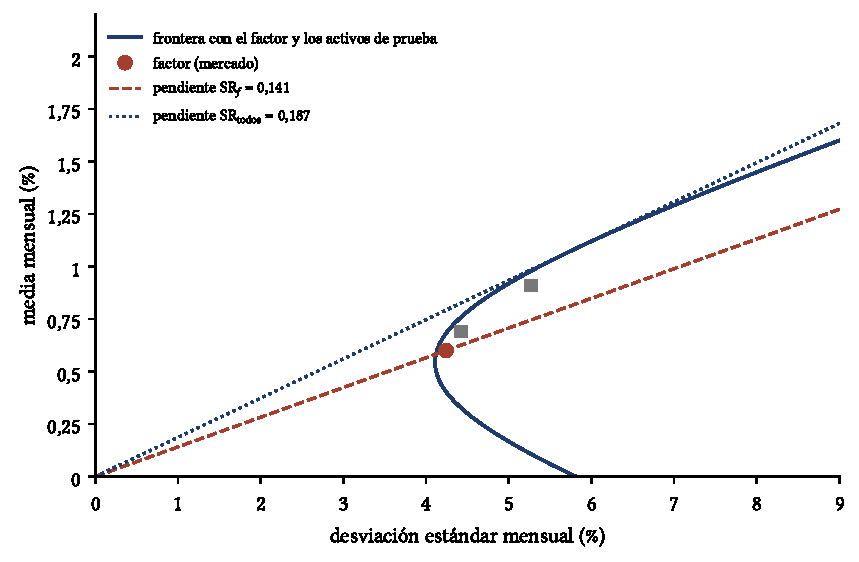
\includegraphics[width=0.72\linewidth]{graficos/cap14_fig_grs.pdf}
\caption{Geometría de la prueba GRS. Con un factor de razón de Sharpe 0,141 y dos activos de prueba con alfas de 0,25 y
0,15 (cuadrados), la cartera tangente alcanza una razón de Sharpe de 0,187. La diferencia entre los cuadrados de ambas
pendientes es exactamente $\boldsymbol\alpha'\Sigma^{-1}\boldsymbol\alpha=0{,}0149$.}
\label{fig:grs}
\end{figure}

% ---------------------------------------------------------------------
\section{Regresiones de corte transversal: Fama-MacBeth}
% ---------------------------------------------------------------------

Cuando los factores no son rendimientos (por ejemplo, el crecimiento del consumo) o cuando se quiere estimar la prima
de cada riesgo directamente, se usa un enfoque de dos pasos. Fama y MacBeth (1973) proponen:
\begin{enumerate}[leftmargin=*]
  \item Estimar las betas de cada cartera con regresiones de series de tiempo: $\hat{\boldsymbol\beta}_i$.
  \item Cada mes $t$, regresar los $N$ excesos de rendimiento sobre las betas:
        $R_{it}=\gamma_{0t}+\hat{\boldsymbol\beta}_i'\boldsymbol\lambda_t+u_{it}$, y promediar en el tiempo:
        \[
          \hat{\boldsymbol\lambda}=\frac1T\sum_{t=1}^{T}\hat{\boldsymbol\lambda}_t,\qquad
          \widehat{\Var}(\hat{\boldsymbol\lambda})=\frac{1}{T^2}\sum_{t=1}^{T}(\hat{\boldsymbol\lambda}_t-\hat{\boldsymbol\lambda})(\hat{\boldsymbol\lambda}_t-\hat{\boldsymbol\lambda})'.
        \]
\end{enumerate}

\begin{proposicion}[Errores estándar de Fama-MacBeth]\label{prop:fm}
Si los $\hat{\boldsymbol\lambda}_t$ no están correlacionados en el tiempo y tienen la misma varianza $V_\lambda$, entonces
$\Var(\hat{\boldsymbol\lambda})=V_\lambda/T$, y el estimador de la proposición es consistente para ella.
\end{proposicion}

\begin{proof}
El promedio de $T$ vectores no correlacionados con varianza común $V_\lambda$ tiene varianza
\begin{align*}
  \Var\Bigl(\frac1T\sum_t\hat{\boldsymbol\lambda}_t\Bigr) &= \frac{1}{T^2}\sum_t\Var(\hat{\boldsymbol\lambda}_t)\\
                                                         &= \frac{1}{T^2}\,T\,V_\lambda\\
                                                         &= \frac{V_\lambda}{T}.
\end{align*}
La varianza muestral de los $\hat{\boldsymbol\lambda}_t$, dividida entre $T$, estima $V_\lambda/T$ de forma consistente. Su
virtud es que incorpora automáticamente la correlación de corte transversal de los errores entre carteras, que una
regresión agrupada ignoraría.
\end{proof}

\paragraph{El problema de las variables generadas.} Las betas del segundo paso son estimaciones con error, y la fórmula
anterior lo ignora. Shanken (1992) muestra que, con betas estimadas en toda la muestra, la varianza correcta es
\[
  \Var(\hat{\boldsymbol\lambda})=\frac1T\Bigl[(X'X)^{-1}X'\Sigma X(X'X)^{-1}\bigl(1+\boldsymbol\lambda'\Omega^{-1}\boldsymbol\lambda\bigr)+\Omega^*\Bigr],
\]
donde $X=(\boldsymbol\iota,\hat B)$ y $\Omega^*$ es la covarianza de los factores bordeada con ceros en la fila y la
columna de la constante. El término $1+\boldsymbol\lambda'\Omega^{-1}\boldsymbol\lambda$ es el mismo que en la
Proposición~\ref{prop:alfas}. Con datos mensuales es pequeño (las razones de Sharpe mensuales lo son), y la corrección
suele cambiar poco los resultados, pero con factores no negociables puede ser grande.

\paragraph{¿Qué mide el $R^2$ de corte transversal?} El ajuste del modelo se juzga comparando los rendimientos promedio
realizados con los ajustados, $\hat\gamma_0+\hat{\boldsymbol\beta}_i'\hat{\boldsymbol\lambda}$. Lewellen, Nagel y Shanken (2010)
advierten que con carteras que tienen una fuerte estructura factorial (como las de tamaño y valor) casi cualquier
factor correlacionado con SMB y HML produce un $R^2$ alto, y recomiendan usar carteras de prueba diversas, como haremos.

% ---------------------------------------------------------------------
\section{Factores estadísticos}
% ---------------------------------------------------------------------

En lugar de proponer factores, pueden extraerse de los datos. Los \emph{componentes principales} de la matriz de
covarianzas $V$ de los rendimientos son las combinaciones lineales $\mathbf v_k'\mathbf R_t$ con los autovectores
$\mathbf v_k$ de $V$, ordenados por su autovalor $\ell_k$. El primero es la combinación de varianza máxima con
$\|\mathbf v\|=1$; el segundo, la de varianza máxima entre las ortogonales al primero, y así sucesivamente. La fracción
$\ell_k/\sum_j\ell_j$ es la parte de la varianza total que explica el componente $k$. La teoría de valoración por
arbitraje (Ross, 1976) justifica que los factores que explican la covarianza sean los que tienen prima; Kozak, Nagel y
Santosh (2018) muestran que los primeros componentes de muchas carteras capturan la mayoría de las anomalías.

% ---------------------------------------------------------------------
\section{Ejercicios resueltos}
% ---------------------------------------------------------------------

\begin{ejresuelto}{CAPM frente a Fama-French}\label{ej:ff3}
\enunciado Estime el CAPM y el modelo de tres factores de Fama y French para las 9 carteras de tamaño y valor.
Compare los alfas y los $R^2$, y la capacidad de cada modelo para explicar la diferencia de rendimiento entre las
acciones pequeñas de valor (S1V5) y las de crecimiento (S1V1).

\solucion
\paso{Paso 1. Resultados.}
\begin{center}\small
\begin{tabular}{@{}lrrrrrrr@{}}
\toprule
 & & \multicolumn{3}{c}{CAPM} & \multicolumn{3}{c}{FF3} \\
\cmidrule(lr){3-5}\cmidrule(lr){6-8}
Cartera & Media & $\hat\alpha$ & $t$ & $R^2$ & $\hat\alpha$ & $t$ & $R^2$ \\
\midrule
S1V1 & 0,344 & $-0{,}547$ & $-3{,}17$ & 0,59 & $-0{,}533$ & $-5{,}14$ & 0,86 \\
S1V3 & 0,833 & 0,137 & 1,17 & 0,65 & $-0{,}049$ & $-0{,}93$ & 0,93 \\
S1V5 & 1,155 & 0,470 & 3,75 & 0,62 & 0,120 & 2,52 & 0,95 \\
S3V1 & 0,625 & $-0{,}200$ & $-1{,}98$ & 0,78 & $-0{,}056$ & $-1{,}08$ & 0,94 \\
S3V3 & 0,839 & 0,190 & 2,56 & 0,80 & 0,006 & 0,11 & 0,90 \\
S3V5 & 1,082 & 0,393 & 3,60 & 0,68 & 0,009 & 0,15 & 0,90 \\
S5V1 & 0,611 & $-0{,}029$ & $-0{,}55$ & 0,89 & 0,136 & 3,57 & 0,94 \\
S5V3 & 0,726 & 0,175 & 2,52 & 0,77 & 0,060 & 1,02 & 0,84 \\
S5V5 & 0,802 & 0,162 & 1,44 & 0,64 & $-0{,}196$ & $-2{,}44$ & 0,82 \\
\bottomrule
\end{tabular}
\end{center}
El promedio de $|\hat\alpha|$ baja de $0{,}256$ a $0{,}129$\,\% mensual y los $R^2$ suben de un rango de 0,59--0,89 a uno de
0,82--0,95. Las cargas en HML van de $-0{,}41$ (crecimiento) a $0{,}84$ (valor), y las de SMB de $-0{,}25$ (grandes) a $1{,}40$
(pequeñas): los factores capturan exactamente las dimensiones con las que se formaron las carteras.

\paso{Paso 2. El diferencial valor-crecimiento.} Las acciones pequeñas de valor rindieron $0{,}811$\,\% mensual más que las de
crecimiento. El CAPM no lo explica; al contrario, como S1V1 tiene más beta (1,38 frente a 1,06), predice que debería rendir
más, y la diferencia de alfas, $0{,}470-(-0{,}547)=1{,}017$, es mayor que la de medias. Con FF3 la diferencia de alfas baja a
$0{,}653$: el modelo explica una parte, pero las acciones pequeñas de crecimiento siguen siendo un caso problemático, con un
alfa de $-0{,}53$\,\% mensual ($t=-5{,}14$), un conocido rompecabezas de la literatura (Figura~\ref{fig:ff3}).

\codigoweb{cap14_ej01}
\salidaR{cap14_ej01_R.txt}
\lectura{cap14_ej01}

\RvsPy Las regresiones de las nueve carteras se resuelven a la vez con un solo sistema $(X'X)B=X'R$, donde cada columna
de $R$ es una cartera; es más rápido y más claro que un bucle de \texttt{lm}. Los excesos de rendimiento se calculan
restando la tasa libre de riesgo, que viene en la misma base: \texttt{as.matrix(...) - f\$RF} en R aprovecha que restar un
vector a una matriz opera por columnas.

\begin{figure}[ht]
\centering
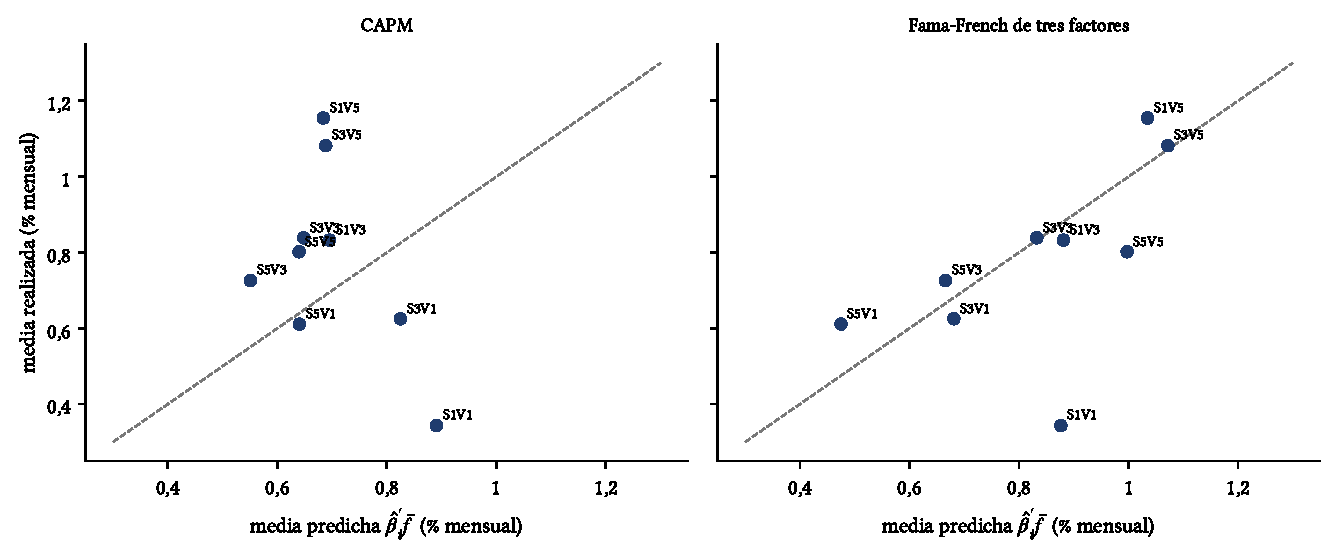
\includegraphics[width=\linewidth]{graficos/cap14_ej01_predicho.pdf}
\caption{Rendimiento medio realizado frente al predicho por cada modelo para las 9 carteras de tamaño y valor. Con un
modelo perfecto, los puntos estarían sobre la diagonal.}
\label{fig:ff3}
\end{figure}

\begin{conclusion}
El modelo de tres factores mejora mucho al CAPM en las carteras de tamaño y valor: reduce los alfas a la mitad y explica
la mayor parte del efecto valor. Pero no lo explica todo, y la cartera de acciones pequeñas de crecimiento sigue lejos
de la diagonal.
\end{conclusion}
\end{ejresuelto}

\begin{ejresuelto}{La prueba GRS}\label{ej:grs}
\enunciado Aplique la prueba GRS al CAPM, al modelo de tres factores y al de cuatro factores de Carhart, con tres conjuntos
de carteras de prueba: tamaño y valor, tamaño y momentum, e industrias.

\solucion
\paso{Paso 1. Resultados.}
\begin{center}\small
\begin{tabular}{@{}llrrr@{}}
\toprule
Carteras & Modelo & $J_{\text{GRS}}$ & Valor $p$ & $|\hat\alpha|$ medio \\
\midrule
Tamaño y valor (9) & CAPM & 7,753 & $5\times10^{-11}$ & 0,256 \\
 & FF3 & 5,754 & $9\times10^{-8}$ & 0,129 \\
 & Carhart & 4,707 & $4\times10^{-6}$ & 0,115 \\
Tamaño y momentum (9) & CAPM & 13,651 & $1\times10^{-20}$ & 0,413 \\
 & FF3 & 12,706 & $5\times10^{-19}$ & 0,425 \\
 & Carhart & 7,858 & $4\times10^{-11}$ & 0,135 \\
Industrias (12) & CAPM & 2,672 & 0,0016 & 0,122 \\
 & FF3 & 5,183 & $2\times10^{-8}$ & 0,167 \\
 & Carhart & 5,082 & $3\times10^{-8}$ & 0,141 \\
\bottomrule
\end{tabular}
\end{center}

\paso{Paso 2. Cálculo para FF3 en tamaño y valor.} Con $T=819$, $N=9$, $L=3$, $\mathrm{SR}^2_f=0{,}05158$ y
$\hat{\boldsymbol\alpha}'\hat\Sigma_{\text{MV}}^{-1}\hat{\boldsymbol\alpha}=0{,}067483$, por la Proposición~\ref{prop:grssharpe}:
\begin{align*}
  J_{\text{GRS}} &= \frac{819-9-3}{9}\cdot\frac{0{,}067483}{1+0{,}05158}\\
                 &= 89{,}667\times0{,}064173\\
                 &= 5{,}754,
\end{align*}
frente a un valor crítico $F_{9,807}$ al 5\,\% de aproximadamente $1{,}89$.

\paso{Paso 3. Interpretación.} Todos los modelos se rechazan con todos los conjuntos: con 69 años de datos la prueba
tiene mucha potencia, y ningún modelo es exactamente cierto. Lo informativo es la comparación. El momentum destruye al
modelo de tres factores: con las carteras de tamaño y momentum, FF3 tiene alfas tan grandes como el CAPM (0,425 frente a
0,413), y solo el factor Mom los reduce a 0,135 (Figura~\ref{fig:alfasmom}). En las industrias, en cambio, agregar SMB y
HML \emph{empeora} el ajuste: los factores de tamaño y valor introducen exposiciones que no se corresponden con
diferencias de rendimiento entre industrias.

\codigoweb{cap14_ej02}
\salidaR{cap14_ej02_R.txt}
\lectura{cap14_ej02}

\RvsPy La matriz $\hat\Omega$ es la covarianza de máxima verosimilitud (dividida entre $T$). En R la calculamos con una
función propia, \texttt{mcov}, porque \texttt{cov} divide entre $T-1$; en Python, \texttt{np.cov(..., bias=True)}. Con un solo
factor, \texttt{np.cov} devuelve un escalar y hay que darle forma de matriz $1\times1$ con \texttt{reshape}.

\begin{figure}[ht]
\centering
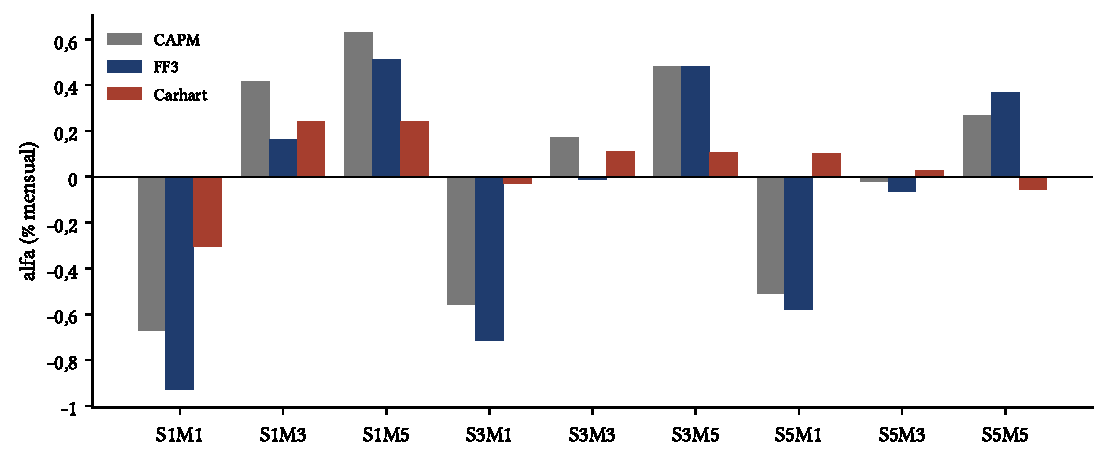
\includegraphics[width=0.88\linewidth]{graficos/cap14_ej02_alfas_momentum.pdf}
\caption{Alfas de las carteras de tamaño y momentum (M1, perdedoras; M5, ganadoras) con cada modelo. Solo el modelo de
Carhart reduce los alfas de las carteras extremas.}
\label{fig:alfasmom}
\end{figure}

\begin{conclusion}
Un modelo de factores debe juzgarse con carteras de prueba que no se hayan formado con sus propias características. El
modelo de tres factores funciona bien donde fue diseñado (tamaño y valor) y mal donde no (momentum, industrias).
\end{conclusion}
\end{ejresuelto}

\begin{ejresuelto}{Primas por riesgo de Fama-MacBeth}\label{ej:fm}
\enunciado Con las 30 carteras, estime las primas por riesgo de los modelos FF3 y Carhart por Fama-MacBeth, con errores
estándar ingenuos y corregidos de Shanken. Compare las primas con las medias de los factores.

\solucion
\paso{Paso 1. FF3.}
\begin{center}\small
\begin{tabular}{@{}lrrrr@{}}
\toprule
 & $\hat\lambda$ & $t$ FM & $t$ Shanken & Media del factor \\
\midrule
Constante & 1,353 & 6,94 & 6,82 & -- \\
Mkt & $-0{,}665$ & $-2{,}70$ & $-2{,}67$ & 0,645 \\
SMB & 0,133 & 1,26 & 1,26 & 0,159 \\
HML & 0,093 & 0,89 & 0,88 & 0,348 \\
\bottomrule
\end{tabular}
\end{center}
El resultado es el contrario del esperado: una constante de 1,35\,\% mensual y una prima de mercado \emph{negativa}, con un
$R^2$ de corte transversal de apenas 0,16. Es el patrón clásico de una línea del mercado de valores demasiado plana:
en el corte transversal, las carteras de más beta no rinden más (Black, Jensen y Scholes, 1972). Si el modelo fuera
correcto, la constante sería cero y cada $\lambda$ igual a la media de su factor.

\paso{Paso 2. Carhart.}
\begin{center}\small
\begin{tabular}{@{}lrrrr@{}}
\toprule
 & $\hat\lambda$ & $t$ FM & $t$ Shanken & Media del factor \\
\midrule
Constante & 0,571 & 3,14 & 3,03 & -- \\
Mkt & 0,150 & 0,64 & 0,63 & 0,645 \\
SMB & 0,102 & 0,97 & 0,97 & 0,159 \\
HML & 0,269 & 2,61 & 2,60 & 0,348 \\
Mom & 0,787 & 5,59 & 5,58 & 0,698 \\
\bottomrule
\end{tabular}
\end{center}
El $R^2$ sube a 0,71 y las primas de HML y Mom quedan cerca de las medias de sus factores (Figura~\ref{fig:fm}). Pero la
constante sigue siendo significativa y la prima de mercado, pequeña.

\paso{Paso 3. La corrección de Shanken.} El término de corrección es $1+\hat{\boldsymbol\lambda}'\hat\Omega^{-1}\hat{\boldsymbol\lambda}=1{,}033$ (FF3) y
$1{,}071$ (Carhart), de modo que los errores estándar de la parte de betas crecen entre 1,6 y 3,5\,\%. Con datos mensuales y
factores negociables la corrección apenas cambia las conclusiones.

\codigoweb{cap14_ej03}
\salidaR{cap14_ej03_R.txt}
\lectura{cap14_ej03}

\RvsPy Las 819 regresiones de corte transversal se resuelven con una sola operación matricial: $(X'X)^{-1}X'R'$ produce una
matriz cuyas columnas son las estimaciones de cada mes. No hace falta ningún bucle. En Python, \texttt{linearmodels} tiene la
clase \texttt{FamaMacBeth}, pero para datos de panel de acciones individuales; para carteras es más transparente
programarlo.

\begin{figure}[ht]
\centering
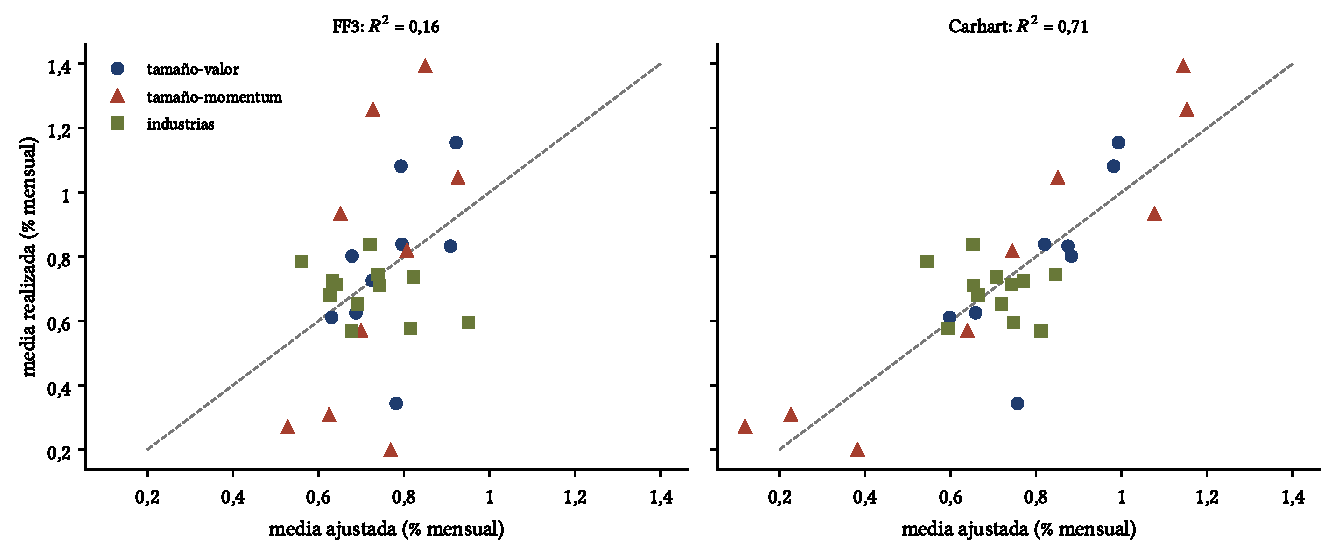
\includegraphics[width=\linewidth]{graficos/cap14_ej03_fama_macbeth.pdf}
\caption{Rendimiento medio realizado frente al ajustado por la regresión de corte transversal, con los modelos FF3 y Carhart,
para las 30 carteras.}
\label{fig:fm}
\end{figure}

\begin{conclusion}
Con carteras de prueba diversas, el modelo de tres factores explica poco del corte transversal de rendimientos; agregar el
momentum lo mejora mucho. La prima de mercado estimada en el corte transversal es casi siempre menor que la del mercado en
el tiempo: las betas altas no se pagan como predice el CAPM.
\end{conclusion}
\end{ejresuelto}

\begin{ejresuelto}{La GRS como razones de Sharpe}\label{ej:grssharpe}
\enunciado Para las 9 carteras de tamaño y valor, verifique numéricamente la Proposición~\ref{prop:grssharpe} con los tres
modelos y compare las razones de Sharpe máximas anuales.

\solucion
\paso{Paso 1. Verificación.} Con el CAPM, la razón de Sharpe mensual del mercado es $0{,}1523$ y la máxima con el mercado y
las 9 carteras, $0{,}3338$:
\begin{align*}
  \mathrm{SR}^2_{\text{todos}}-\mathrm{SR}^2_f &= 0{,}3338^2-0{,}1523^2\\
                                                &= 0{,}11142-0{,}02320\\
                                                &= 0{,}08822\approx0{,}088249,
\end{align*}
que coincide (con todas las decimales en la salida) con $\hat{\boldsymbol\alpha}'\hat\Sigma_{\text{MV}}^{-1}\hat{\boldsymbol\alpha}$. Lo mismo ocurre con FF3
($0{,}067483$) y Carhart ($0{,}058279$).

\paso{Paso 2. Razones de Sharpe anuales.} Multiplicando por $\sqrt{12}$:
\begin{center}\small
\begin{tabular}{@{}lrr@{}}
\toprule
Modelo & Solo factores & Factores y 9 carteras \\
\midrule
CAPM    & 0,528 & 1,156 \\
FF3     & 0,787 & 1,195 \\
Carhart & 1,143 & 1,417 \\
\bottomrule
\end{tabular}
\end{center}
Agregar factores acerca la frontera de los factores a la de todos los activos, pero la brecha nunca se cierra
(Figura~\ref{fig:sharpe}). Por separado, el factor de mayor razón de Sharpe mensual es Mom ($0{,}179$), seguido del mercado
($0{,}152$), HML ($0{,}129$) y SMB ($0{,}056$).

\codigoweb{cap14_ej04}
\salidaR{cap14_ej04_R.txt}
\lectura{cap14_ej04}

\RvsPy La identidad es exacta en la muestra solo si las covarianzas se calculan dividiendo entre $T$; con la covarianza
insesgada habría una discrepancia en la cuarta cifra. En ambos lenguajes, $\mathbf m'V^{-1}\mathbf m$ se calcula con
\texttt{solve} en lugar de invertir $V$, que es más estable numéricamente.

\begin{figure}[ht]
\centering
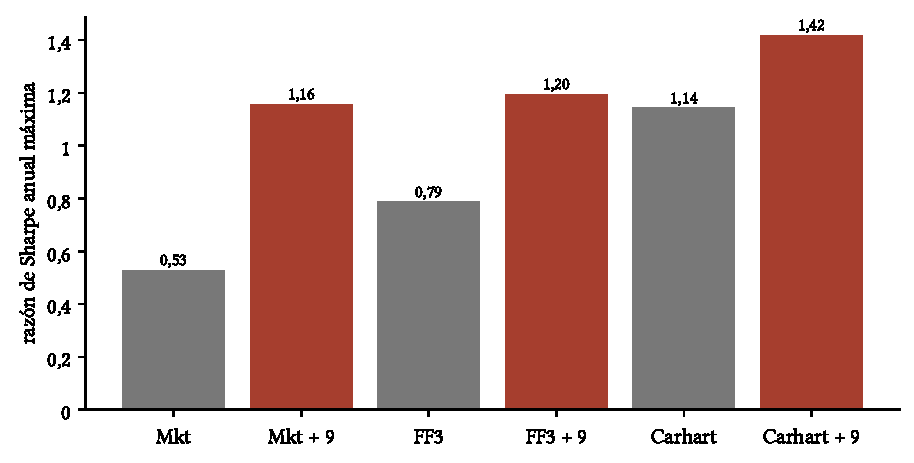
\includegraphics[width=0.72\linewidth]{graficos/cap14_ej04_sharpe.pdf}
\caption{Razón de Sharpe anual máxima con cada conjunto de factores (gris) y al agregar las 9 carteras de tamaño y valor
(rojo). La diferencia de los cuadrados es lo que mide la prueba GRS.}
\label{fig:sharpe}
\end{figure}

\begin{conclusion}
Rechazar un modelo con la prueba GRS significa que existe una cartera de los activos de prueba que mejora la razón de
Sharpe de los factores. En estos datos, la mejora es grande para el CAPM (de 0,53 a 1,16 anual) y menor, pero aún
significativa, para el modelo de Carhart.
\end{conclusion}
\end{ejresuelto}

\begin{ejresuelto}{Componentes principales}\label{ej:pca}
\enunciado Extraiga los componentes principales de la matriz de covarianzas de las 30 carteras. ¿Qué parte de la varianza
explican? ¿Con qué factores se relacionan los tres primeros?

\solucion
\paso{Paso 1. Varianza explicada.} El primer componente explica el 73,46\,\% de la varianza total; el segundo, el 6,29\,\%; el
tercero, el 4,01\,\%. Los tres primeros, el 83,76\,\%. Hay una fuerte estructura factorial: un solo factor domina.

\paso{Paso 2. Interpretación.}
\begin{center}\small
\begin{tabular}{@{}lrrrrr@{}}
\toprule
 & Mkt & SMB & HML & Mom & $R^2$ con los cuatro \\
\midrule
CP1 & 0,962 & 0,462 & $-0{,}128$ & $-0{,}206$ & 0,989 \\
CP2 & 0,217 & $-0{,}801$ & 0,056 & 0,010 & 0,836 \\
CP3 & 0,107 & 0,094 & $-0{,}562$ & 0,855 & 0,916 \\
\bottomrule
\end{tabular}
\end{center}
El primer componente es casi el mercado (correlación 0,96; todas las cargas positivas). El segundo es un factor de tamaño,
con signo opuesto a SMB: contrapone acciones grandes y pequeñas. El tercero mezcla momentum y valor con signos opuestos, lo
que refleja la conocida correlación negativa entre ambas estrategias (Figura~\ref{fig:pca}).

\paso{Paso 3. Ajuste.} Tres componentes producen un $R^2$ medio de series de tiempo de 0,817 en las 30 carteras, algo más que
Mkt, SMB y HML (0,794). Los componentes están diseñados para explicar la covarianza; no garantizan explicar los
\emph{rendimientos medios}, que es lo que importa para la valoración.

\codigoweb{cap14_ej05}
\salidaR{cap14_ej05_R.txt}
\lectura{cap14_ej05}

\RvsPy El signo de un autovector es arbitrario: \texttt{eigen} de R y \texttt{np.linalg.eigh} de Python pueden devolver
signos opuestos. Para que los resultados coincidan, normalizamos cada autovector para que la suma de sus cargas sea
positiva. Además, \texttt{eigh} ordena los autovalores de menor a mayor y \texttt{eigen} de mayor a menor.

\begin{figure}[ht]
\centering
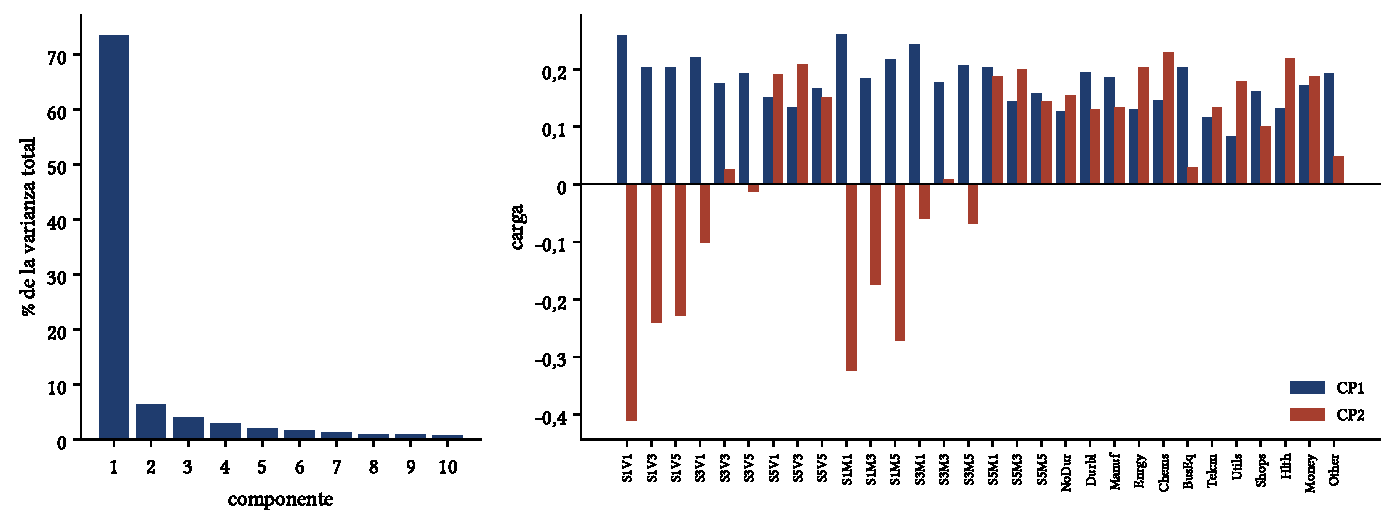
\includegraphics[width=\linewidth]{graficos/cap14_ej05_componentes.pdf}
\caption{Izquierda: fracción de la varianza explicada por los diez primeros componentes. Derecha: cargas de los dos primeros
componentes en las 30 carteras; el primero carga positivamente en todas y el segundo separa pequeñas de grandes.}
\label{fig:pca}
\end{figure}

\begin{conclusion}
Los datos encuentran por sí solos un factor de mercado y uno de tamaño, y un tercero relacionado con momentum y valor. Los
factores económicos de Fama, French y Carhart son, en buena medida, rotaciones de los factores estadísticos dominantes.
\end{conclusion}
\end{ejresuelto}

% ---------------------------------------------------------------------
\section{Ejercicios propuestos}
% ---------------------------------------------------------------------

\begin{enumerate}[label=\textbf{\thechapter.\arabic*},leftmargin=*,itemsep=6pt]
  \item Con $T=600$, $N=25$, $L=3$, $\mathrm{SR}^2_f=0{,}04$ y $\hat{\boldsymbol\alpha}'\hat\Sigma_{\text{MV}}^{-1}\hat{\boldsymbol\alpha}=0{,}06$, calcule el
  estadístico GRS. \textit{Respuesta: $1{,}320$.}

  \item Demuestre que, en el CAPM con un solo factor, $1+\mathrm{SR}^2_f=1+\bar f^2/\hat\sigma_f^2$ y que el error estándar del alfa
  es $\hat\sigma_\varepsilon\sqrt{(1+\bar f^2/\hat\sigma_f^2)/T}$.

  \item Verifique que $V=GDG'$ en la demostración de la Proposición~\ref{prop:grssharpe}.

  \item Demuestre que el primer componente principal maximiza $\mathbf v'V\mathbf v$ sujeto a $\mathbf v'\mathbf v=1$ y que el
  máximo es el mayor autovalor de $V$.

  \item ¿Por qué un factor negociable debe tener una prima igual a su media? (Sugerencia: aplique el modelo al propio factor.)

  \item \emph{(Simulación.)} Simule 1\,000 muestras de $T=240$ meses de 10 carteras que cumplen exactamente el CAPM, con betas
  entre 0,5 y 1,5. Calcule la frecuencia de rechazos de la GRS al 5\,\% y de al menos un $t$ individual mayor que 1,96. ¿Por
  qué difieren?

  \item \emph{(Con datos de Yahoo Finance.)} Forme carteras de acciones de la Bolsa de Valores de Lima por tamaño y estime el
  CAPM con el índice S\&P/BVL Perú General como mercado. ¿Hay efecto tamaño en el mercado peruano?

  \item \emph{(Con datos.)} Divida la muestra en 1949--1983 y 1984--2017 y repita el Ejercicio~\ref{ej:fm}. ¿Es estable la prima de
  momentum?
\end{enumerate}

% ---------------------------------------------------------------------
\section{Resumen de fórmulas}
% ---------------------------------------------------------------------

\begin{table}[H]
\centering\small
\begin{tabular}{@{}ll@{}}
\toprule
Concepto & Fórmula \\
\midrule
Modelo de series de tiempo & $R_{it}=\alpha_i+\boldsymbol\beta_i'\mathbf f_t+\varepsilon_{it}$;\quad $H_0$: $\boldsymbol\alpha=\mathbf 0$ \\
Varianza de los alfas & $(1+\hat{\boldsymbol\mu}'\hat\Omega^{-1}\hat{\boldsymbol\mu})\Sigma/T$ \\
GRS & $\frac{T-N-L}{N}\frac{T}{T-L-1}\frac{\hat{\boldsymbol\alpha}'\hat\Sigma^{-1}\hat{\boldsymbol\alpha}}{1+\hat{\boldsymbol\mu}'\hat\Omega^{-1}\hat{\boldsymbol\mu}}\sim F_{N,T-N-L}$ \\
GRS y Sharpe & $\hat{\boldsymbol\alpha}'\hat\Sigma_{\text{MV}}^{-1}\hat{\boldsymbol\alpha}=\mathrm{SR}^2_{\text{todos}}-\mathrm{SR}^2_f$ \\
Fama-MacBeth & $\hat{\boldsymbol\lambda}=\frac1T\sum_t\hat{\boldsymbol\lambda}_t$;\quad $\widehat{\Var}=\frac{1}{T^2}\sum_t(\hat{\boldsymbol\lambda}_t-\hat{\boldsymbol\lambda})(\cdot)'$ \\
Shanken & $\frac1T[(X'X)^{-1}X'\Sigma X(X'X)^{-1}(1+\boldsymbol\lambda'\Omega^{-1}\boldsymbol\lambda)+\Omega^*]$ \\
Componentes principales & $V\mathbf v_k=\ell_k\mathbf v_k$;\quad varianza explicada $\ell_k/\sum_j\ell_j$ \\
\bottomrule
\end{tabular}
\caption{Fórmulas principales del Capítulo 14.}
\end{table}

\section*{Referencias}
\begin{itemize}[leftmargin=*]
  \item Black, F., Jensen, M. C. y Scholes, M. (1972). The capital asset pricing model: Some empirical tests. En M. C. Jensen
        (ed.), \emph{Studies in the Theory of Capital Markets}, 79--121. Praeger.
  \item Carhart, M. M. (1997). On persistence in mutual fund performance. \emph{Journal of Finance}, 52(1), 57--82.
  \item Cochrane, J. H. (2005). \emph{Asset Pricing}, ed. revisada. Princeton University Press.
  \item Fama, E. F. y French, K. R. (1993). Common risk factors in the returns on stocks and bonds. \emph{Journal of Financial
        Economics}, 33(1), 3--56.
  \item Fama, E. F. y MacBeth, J. D. (1973). Risk, return, and equilibrium: Empirical tests. \emph{Journal of Political
        Economy}, 81(3), 607--636.
  \item Gibbons, M. R., Ross, S. A. y Shanken, J. (1989). A test of the efficiency of a given portfolio. \emph{Econometrica},
        57(5), 1121--1152.
  \item Kozak, S., Nagel, S. y Santosh, S. (2018). Interpreting factor models. \emph{Journal of Finance}, 73(3), 1183--1223.
  \item Lewellen, J., Nagel, S. y Shanken, J. (2010). A skeptical appraisal of asset pricing tests. \emph{Journal of Financial
        Economics}, 96(2), 175--194.
  \item Ross, S. A. (1976). The arbitrage theory of capital asset pricing. \emph{Journal of Economic Theory}, 13(3), 341--360.
  \item Shanken, J. (1992). On the estimation of beta-pricing models. \emph{Review of Financial Studies}, 5(1), 1--33.
\end{itemize}

% =====================================================================
%  Capítulo 15. Estructura temporal de las tasas de interés
% =====================================================================
\chapter[Estructura temporal de tasas]{Estructura temporal de las tasas de interés: expectativas, Nelson-Siegel y Vasicek}\label{cap:tasas}

\section*{Objetivos de aprendizaje}
Al terminar este capítulo, el lector podrá:
\begin{enumerate}[label=\arabic*.,leftmargin=*]
  \item Pasar entre precios de bonos cupón cero, rendimientos, tasas a plazo y rendimientos de mantener un bono, y
        demostrar las identidades que los unen.
  \item Contrastar la hipótesis de las expectativas con las regresiones de Campbell y Shiller y de Fama y Bliss, y
        entender por qué su rechazo implica primas por plazo variables.
  \item Resumir la curva con tres factores, ya sea estadísticos (componentes principales) o paramétricos (Nelson-Siegel
        en la versión dinámica de Diebold y Li).
  \item Estimar el modelo de Vasicek a partir de su discretización exacta y detectar el efecto nivel en la volatilidad
        (modelo CKLS).
\end{enumerate}

\section*{Motivación}
Un banco central fija la tasa a un día; los hogares y las empresas se endeudan a plazos de meses o de años. Lo que une
ambos extremos es la curva de rendimientos: la relación, en una fecha dada, entre el plazo de un bono y su
rendimiento. Su forma resume lo que el mercado espera de las tasas futuras y lo que cobra por cargar con el riesgo de
plazo. Una curva con pendiente negativa ha precedido a la mayoría de las recesiones de Estados Unidos desde la
posguerra, y los tesoreros, los fondos de pensiones y los reguladores la usan a diario para valorar flujos futuros.
Este capítulo trata la curva como un objeto econométrico: un vector de series de tiempo muy persistentes y muy
correlacionadas, con una estructura de factores fuerte y con restricciones teóricas que se pueden contrastar.

\paragraph{Datos del capítulo.} Rendimientos de bonos cupón cero del Tesoro de Estados Unidos, en porcentaje anual, a
fin de cada mes, de diciembre de 1946 a febrero de 1991 ($T=531$), para diez vencimientos: 1, 2, 3, 5, 6, 11, 12, 36, 60
y 120 meses. Son las curvas estimadas por McCulloch y Kwon (1993) a partir de precios de bonos con cupón, distribuidas en
la colección \texttt{Rdatasets} (conjunto \texttt{Irates} del paquete \texttt{Ecdat}). Es la misma clase de datos que usan
Campbell y Shiller (1991). En el texto los tratamos como rendimientos compuestos en forma continua. Para la curva soberana
peruana, el BCRP publica rendimientos por plazo que permiten repetir los ejercicios (Ejercicio propuesto 15.7).

% ---------------------------------------------------------------------
\section{Precios, rendimientos y tasas a plazo}
% ---------------------------------------------------------------------

Sea $P_{n,t}$ el precio en $t$ de un bono cupón cero que paga una unidad dentro de $n$ períodos. Su rendimiento
(compuesto en forma continua, por período) $y_{n,t}$ es la tasa constante que descuenta ese pago al precio de mercado:
\[
  P_{n,t}=e^{-n\,y_{n,t}},\qquad y_{n,t}=-\frac{1}{n}\ln P_{n,t}.
\]
La \emph{curva de rendimientos} en la fecha $t$ es la función $n\mapsto y_{n,t}$. Con $p_{n,t}=\ln P_{n,t}$ escribimos
$p_{n,t}=-n\,y_{n,t}$.

\begin{definicion}[Tasa a plazo]
La tasa a plazo $f_t(n,m)$, con $n<m$, es la tasa que hoy se puede asegurar para prestar entre $t+n$ y $t+m$. La tasa a
plazo de un período que empieza en $t+n-1$ se escribe $f_t(n)=f_t(n-1,n)$.
\end{definicion}

\begin{proposicion}[Tasa a plazo implícita]\label{prop:plazo}
En ausencia de arbitraje,
\[
  f_t(n,m)=\frac{m\,y_{m,t}-n\,y_{n,t}}{m-n},\qquad f_t(n)=n\,y_{n,t}-(n-1)\,y_{n-1,t}.
\]
\end{proposicion}

\begin{proof}
Hay dos formas de llevar una unidad de hoy hasta $t+m$. La primera es comprar bonos de $m$ períodos. La segunda es
comprar bonos de $n$ períodos y, al mismo tiempo, pactar hoy un préstamo a la tasa $f_t(n,m)$ entre $t+n$ y $t+m$.
Ambas estrategias no tienen riesgo, así que deben rendir lo mismo:
\begin{align*}
  e^{m\,y_{m,t}} &= e^{n\,y_{n,t}}\,e^{(m-n)f_t(n,m)}\\
  m\,y_{m,t}     &= n\,y_{n,t}+(m-n)\,f_t(n,m)\\
  (m-n)\,f_t(n,m) &= m\,y_{m,t}-n\,y_{n,t}\\
  f_t(n,m)       &= \frac{m\,y_{m,t}-n\,y_{n,t}}{m-n}.
\end{align*}
Para la tasa de un período, tomamos $m=n$ y $n-1$ en lugar de $n$:
\begin{align*}
  f_t(n) &= \frac{n\,y_{n,t}-(n-1)\,y_{n-1,t}}{n-(n-1)}\\
         &= n\,y_{n,t}-(n-1)\,y_{n-1,t}.
\end{align*}
\end{proof}

La fórmula también dice que el rendimiento es el promedio de las tasas a plazo de un período:
\[
  y_{n,t}=\frac1n\sum_{i=1}^{n}f_t(i),\qquad f_t(1)=y_{1,t},
\]
pues la suma de $f_t(i)=i\,y_{i,t}-(i-1)\,y_{i-1,t}$ es telescópica. Cuando la curva sube, las tasas a plazo están por encima
de los rendimientos; cuando baja, por debajo.

\begin{definicion}[Rendimiento de mantener un bono]
El rendimiento logarítmico de comprar en $t$ un bono de $n$ períodos y venderlo en $t+1$, cuando le quedan $n-1$, es
$h_{t+1}(n)=p_{n-1,t+1}-p_{n,t}$. Su exceso sobre la tasa de un período es $rx_{t+1}(n)=h_{t+1}(n)-y_{1,t}$.
\end{definicion}

\begin{proposicion}[Descomposición del rendimiento en exceso]\label{prop:rx}
\[
  rx_{t+1}(n)=\bigl[f_t(n)-y_{1,t}\bigr]-(n-1)\bigl[y_{n-1,t+1}-y_{n-1,t}\bigr].
\]
\end{proposicion}

\begin{proof}
Partimos de la definición y sustituimos $p=-n\,y$:
\begin{align*}
  rx_{t+1}(n) &= p_{n-1,t+1}-p_{n,t}-y_{1,t}\\
              &= -(n-1)\,y_{n-1,t+1}+n\,y_{n,t}-y_{1,t}.
\end{align*}
Sumamos y restamos $(n-1)\,y_{n-1,t}$:
\begin{align*}
  rx_{t+1}(n) &= n\,y_{n,t}-(n-1)\,y_{n-1,t}-y_{1,t}-(n-1)\,y_{n-1,t+1}+(n-1)\,y_{n-1,t}\\
              &= \bigl[f_t(n)-y_{1,t}\bigr]-(n-1)\bigl[y_{n-1,t+1}-y_{n-1,t}\bigr],
\end{align*}
donde el último paso usa la Proposición~\ref{prop:plazo}.
\end{proof}

El rendimiento en exceso tiene una parte conocida en $t$, el diferencial entre la tasa a plazo y la tasa corta, y una
parte aleatoria: la pérdida de capital si el rendimiento sube. El factor $(n-1)$ es la duración del bono al venderlo; por
eso los bonos largos son mucho más volátiles que los cortos.

% ---------------------------------------------------------------------
\section{La hipótesis de las expectativas}
% ---------------------------------------------------------------------

La hipótesis de las expectativas (HE) afirma que los rendimientos largos son el promedio de las tasas cortas esperadas,
más una prima por plazo que puede depender del vencimiento pero \emph{no del tiempo}:
\[
  y_{n,t}=\frac1n\sum_{i=0}^{n-1}\E_t\bigl[y_{1,t+i}\bigr]+c_n .
\]
Una forma equivalente es que el rendimiento en exceso esperado de cualquier bono es constante:
$\E_t[rx_{t+1}(n)]=\text{constante}$. La HE tiene tres implicaciones contrastables.

\begin{proposicion}[Tasas cortas futuras]\label{prop:he1}
Sea $k=hm$, con $h$ entero. Bajo la HE, en la regresión
\[
  \frac1h\sum_{i=0}^{h-1}y_{m,t+mi}-y_{m,t}=a+b\,\bigl(y_{k,t}-y_{m,t}\bigr)+u_{t+k-m},
\]
el coeficiente poblacional es $b=1$.
\end{proposicion}

\begin{proof}
Aplicada a bonos de $k$ períodos y de $m$ períodos que se renuevan $h$ veces, la HE dice que
$y_{k,t}=\frac1h\sum_{i=0}^{h-1}\E_t[y_{m,t+mi}]+c$, con $c$ constante. Llamemos $Z_t$ al lado izquierdo de la regresión y
$S_t=y_{k,t}-y_{m,t}$ a la pendiente. Entonces
\begin{align*}
  \E_t[Z_t] &= \frac1h\sum_{i=0}^{h-1}\E_t[y_{m,t+mi}]-y_{m,t}\\
            &= y_{k,t}-c-y_{m,t}\\
            &= S_t-c .
\end{align*}
El error de predicción $u_t=Z_t-\E_t[Z_t]$ no está correlacionado con nada conocido en $t$, y $S_t$ se conoce en $t$. Por
tanto,
\begin{align*}
  \Cov(Z_t,S_t) &= \Cov\bigl(\E_t[Z_t]+u_t,\ S_t\bigr)\\
                &= \Cov(S_t-c,\ S_t)+\Cov(u_t,S_t)\\
                &= \Var(S_t)+0,
\end{align*}
y el coeficiente de MCO en la población es $b=\Cov(Z_t,S_t)/\Var(S_t)=1$.
\end{proof}

\begin{proposicion}[Regresión de la tasa larga de Campbell y Shiller]\label{prop:he2}
Bajo la HE, en la regresión
\[
  y_{n-1,t+1}-y_{n,t}=a+b\,\frac{y_{n,t}-y_{1,t}}{n-1}+u_{t+1}
\]
el coeficiente poblacional es $b=1$: cuando la curva tiene pendiente positiva, el rendimiento largo debe \emph{subir}.
\end{proposicion}

\begin{proof}
La HE con primas constantes implica que el rendimiento de mantener el bono largo un período iguala, en esperanza, a la
tasa corta más una constante: $\E_t[h_{t+1}(n)]=y_{1,t}+c$. Usando $h_{t+1}(n)=n\,y_{n,t}-(n-1)\,y_{n-1,t+1}$:
\begin{align*}
  n\,y_{n,t}-(n-1)\,\E_t[y_{n-1,t+1}] &= y_{1,t}+c\\
  (n-1)\,\E_t[y_{n-1,t+1}]            &= n\,y_{n,t}-y_{1,t}-c\\
  \E_t[y_{n-1,t+1}]-y_{n,t}           &= \frac{n\,y_{n,t}-y_{1,t}-c}{n-1}-\frac{(n-1)\,y_{n,t}}{n-1}\\
                                      &= \frac{y_{n,t}-y_{1,t}}{n-1}-\frac{c}{n-1}.
\end{align*}
Igual que en la proposición anterior, el error de predicción no está correlacionado con la pendiente, y el coeficiente
es $b=1$.
\end{proof}

La intuición es la de un arbitraje: si el bono largo rinde más que el corto por su cupón implícito, la única forma de
que ambos tengan el mismo rendimiento esperado es que el largo sufra una pérdida de capital, es decir, que su rendimiento
suba.

\begin{corolario}[Regresión de Fama y Bliss]\label{cor:fb}
Bajo la HE, en la regresión $rx_{t+1}(n)=a+b\,[f_t(n)-y_{1,t}]+u_{t+1}$ el coeficiente es $b=0$.
\end{corolario}

\begin{proof}
Bajo la HE, $\E_t[rx_{t+1}(n)]$ es una constante. Una constante no está correlacionada con ninguna variable conocida en
$t$, en particular con el diferencial a plazo:
\begin{align*}
  \Cov\bigl(rx_{t+1}(n),\ f_t(n)-y_{1,t}\bigr) &= \Cov\bigl(\E_t[rx_{t+1}(n)]+u_{t+1},\ f_t(n)-y_{1,t}\bigr)\\
                                               &= 0+0 .
\end{align*}
\end{proof}

Las tres regresiones son caras de la misma hipótesis. Por la Proposición~\ref{prop:rx}, si en la de Campbell y Shiller el
coeficiente es menor que uno, el rendimiento largo no sube lo suficiente, el bono largo rinde más cuando la pendiente es
alta y en la de Fama y Bliss el coeficiente es positivo. En ambos casos la conclusión es que la prima por plazo
\emph{varía en el tiempo} y es predecible con la forma de la curva.

\begin{observacion}
Cuando el horizonte $k$ es mayor que la frecuencia de los datos, los lados izquierdos de meses consecutivos comparten
$k-m$ observaciones: los errores siguen un MA$(k-m)$ incluso bajo la hipótesis nula. Por eso se usan errores estándar de
Newey-West con al menos $k-m$ rezagos (Capítulo~\ref{cap:robustos}). Además, las regresiones de pendiente sufren un sesgo
de muestra finita, porque el regresor es muy persistente; con horizontes de diez años y 44 años de datos hay apenas cuatro
observaciones independientes.
\end{observacion}

% ---------------------------------------------------------------------
\section{Modelos de factores de la curva}
% ---------------------------------------------------------------------

Diez rendimientos que se mueven casi juntos son una matriz de covarianzas casi de rango bajo. Litterman y Scheinkman
(1991) mostraron que tres componentes principales, a los que llamaron \emph{nivel}, \emph{pendiente} y \emph{curvatura},
explican más del 95\,\% de la variación de los rendimientos. El Ejercicio~\ref{ej:curva} lo verifica.

\subsection*{Nelson-Siegel}
Nelson y Siegel (1987) propusieron una forma paramétrica para la curva en una fecha:
\[
  y(\tau)=\beta_0+\beta_1\,\frac{1-e^{-\lambda\tau}}{\lambda\tau}
          +\beta_2\Bigl(\frac{1-e^{-\lambda\tau}}{\lambda\tau}-e^{-\lambda\tau}\Bigr).
\]
Diebold y Li (2006) la volvieron dinámica: fijan $\lambda$ y dejan que los tres coeficientes varíen cada mes,
$\boldsymbol\beta_t=(\beta_{0t},\beta_{1t},\beta_{2t})'$. Con $\lambda$ fijo, la curva es lineal en $\boldsymbol\beta_t$, que se
estima por MCO de corte transversal fecha por fecha.

\begin{proposicion}[Interpretación de las cargas]\label{prop:ns}
Para $\lambda>0$:
\begin{enumerate}[label=(\alph*)]
  \item $\displaystyle\lim_{\tau\to\infty}y(\tau)=\beta_0$: $\beta_0$ es el nivel de largo plazo.
  \item $\displaystyle\lim_{\tau\to0}y(\tau)=\beta_0+\beta_1$: la tasa instantánea; $-\beta_1$ es la pendiente
        (largo menos corto).
  \item La carga de $\beta_2$ vale cero en ambos extremos y tiene un único máximo en $\lambda\tau=x^*\approx1{,}7933$.
\end{enumerate}
\end{proposicion}

\begin{proof}
Escribimos $x=\lambda\tau$ y $s(x)=(1-e^{-x})/x$.

(a) Cuando $x\to\infty$, $e^{-x}\to0$:
\begin{align*}
  s(x) &= \frac{1-e^{-x}}{x}\ \to\ \frac{1-0}{\infty}=0,\\
  s(x)-e^{-x} &\to 0-0=0,\\
  y(\tau) &\to \beta_0+\beta_1\cdot0+\beta_2\cdot0=\beta_0 .
\end{align*}

(b) Cuando $x\to0$, usamos $e^{-x}=1-x+\frac{x^2}{2}+O(x^3)$:
\begin{align*}
  1-e^{-x} &= x-\frac{x^2}{2}+O(x^3)\\
  s(x)     &= 1-\frac{x}{2}+O(x^2)\ \to\ 1,\\
  s(x)-e^{-x} &\to 1-1=0,\\
  y(\tau)  &\to \beta_0+\beta_1\cdot1+\beta_2\cdot0=\beta_0+\beta_1 .
\end{align*}

(c) Sea $g(x)=s(x)-e^{-x}$. Por (a) y (b), $g(x)\to0$ en ambos extremos, y $g(x)>0$ para $x>0$ porque
$1-e^{-x}>x\,e^{-x}$ (equivale a $e^{x}>1+x$). Su derivada es
\begin{align*}
  g'(x) &= \frac{x\,e^{-x}-(1-e^{-x})}{x^2}+e^{-x}\\
        &= \frac{x\,e^{-x}-1+e^{-x}+x^2e^{-x}}{x^2}\\
        &= \frac{e^{-x}\,(x^2+x+1)-1}{x^2}.
\end{align*}
El numerador $q(x)=e^{-x}(x^2+x+1)-1$ vale cero en $x=0$ y su derivada es
\begin{align*}
  q'(x) &= -e^{-x}(x^2+x+1)+e^{-x}(2x+1)\\
        &= e^{-x}\,(x-x^2)\\
        &= e^{-x}\,x\,(1-x),
\end{align*}
positiva en $(0,1)$ y negativa en $(1,\infty)$. Así $q$ sube desde cero hasta $x=1$ y luego decrece hacia $-1$: cruza el
cero una sola vez, en $x^*>1$. Ese cruce es el único punto crítico de $g$, y como $g$ es positiva y se anula en los
extremos, es un máximo. Numéricamente, $x^*=1{,}7933$.
\end{proof}

Diebold y Li eligen $\lambda=0{,}0609$ (con $\tau$ en meses) para que la carga de curvatura sea máxima en
$\tau=1{,}7933/0{,}0609=29{,}45$ meses, entre los dos y los tres años. La Figura~\ref{fig:ns} muestra las tres cargas y las
formas de curva que generan: con $\beta_1<0$ la curva sube, con $\beta_1>0$ se invierte y con $\beta_2>0$ aparece una
joroba en los plazos medios.

\begin{figure}[ht]
\centering
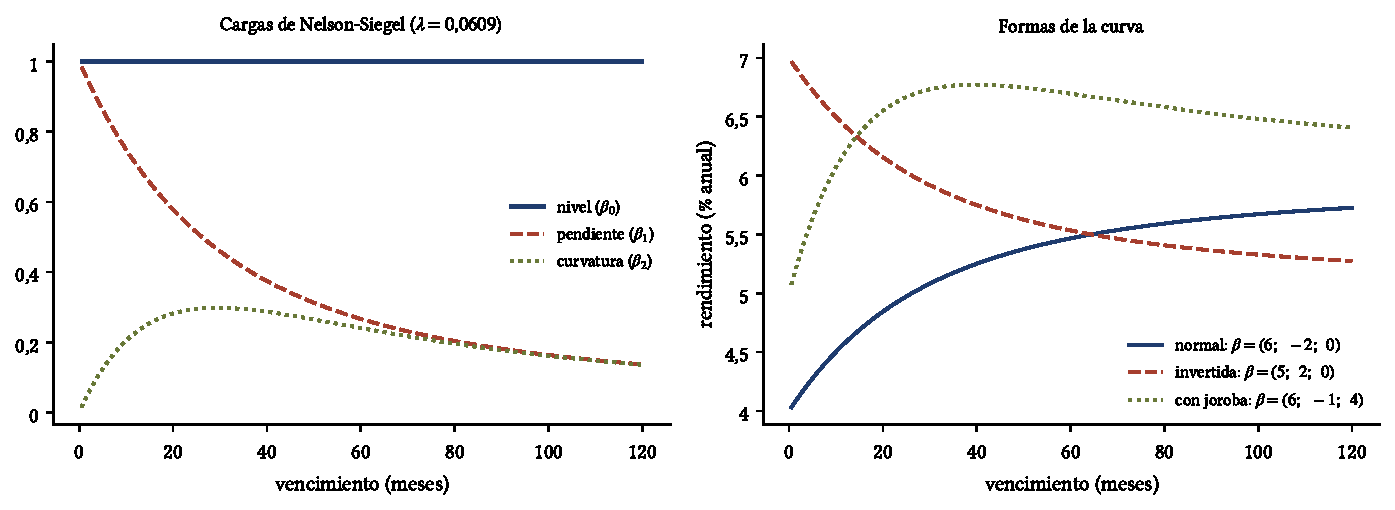
\includegraphics[width=\linewidth]{graficos/cap15_fig_nelson_siegel.pdf}
\caption{Izquierda: cargas de Nelson-Siegel con $\lambda=0{,}0609$. La de nivel es constante, la de pendiente cae de 1 a 0
y la de curvatura alcanza su máximo, 0,2984, en $\tau=29{,}45$ meses. Derecha: tres curvas generadas con distintos
$\boldsymbol\beta$.}
\label{fig:ns}
\end{figure}

\begin{observacion}
La versión de Diebold y Li no impone la ausencia de arbitraje entre vencimientos. Christensen, Diebold y Rudebusch
(2011) muestran que agregar un pequeño término de ajuste por convexidad la vuelve libre de arbitraje sin perder su
ajuste. Para pronosticar, Diebold y Li modelan cada $\beta_{jt}$ como un AR(1), algo que solo tiene sentido si los factores
son persistentes, como se verifica en el Ejercicio~\ref{ej:ns}.
\end{observacion}

% ---------------------------------------------------------------------
\section{Modelos de la tasa corta: Vasicek y CKLS}
% ---------------------------------------------------------------------

Los modelos de equilibrio parten de la dinámica de la tasa instantánea $r_t$. Vasicek (1977) propuso un proceso de
Ornstein-Uhlenbeck:
\[
  dr_t=\kappa(\theta-r_t)\,dt+\sigma\,dW_t,\qquad \kappa>0 .
\]
La tasa vuelve hacia $\theta$ con una velocidad proporcional a la distancia, y $\sigma$ es la volatilidad.

\begin{proposicion}[Discretización exacta de Vasicek]\label{prop:vasicek}
Para un intervalo $\Delta>0$,
\[
  r_{t+\Delta}=\theta+e^{-\kappa\Delta}(r_t-\theta)+\varepsilon_{t+\Delta},\qquad
  \varepsilon_{t+\Delta}\sim N\!\Bigl(0,\ \sigma^2\,\frac{1-e^{-2\kappa\Delta}}{2\kappa}\Bigr),
\]
y los $\varepsilon$ de intervalos disjuntos son independientes. Es decir, $r$ muestreado cada $\Delta$ es un AR(1)
$r_{t+\Delta}=a+b\,r_t+\varepsilon$ con
\[
  b=e^{-\kappa\Delta},\qquad a=\theta(1-b),\qquad \Var(\varepsilon)=s^2=\sigma^2\,\frac{1-b^2}{2\kappa}.
\]
\end{proposicion}

\begin{proof}
Sea $Z_t=e^{\kappa t}(r_t-\theta)$. Por el lema de Itô, como $Z$ es lineal en $r$:
\begin{align*}
  dZ_t &= \kappa e^{\kappa t}(r_t-\theta)\,dt+e^{\kappa t}\,dr_t\\
       &= \kappa e^{\kappa t}(r_t-\theta)\,dt+e^{\kappa t}\bigl[\kappa(\theta-r_t)\,dt+\sigma\,dW_t\bigr]\\
       &= \kappa e^{\kappa t}(r_t-\theta)\,dt-\kappa e^{\kappa t}(r_t-\theta)\,dt+\sigma e^{\kappa t}\,dW_t\\
       &= \sigma e^{\kappa t}\,dW_t .
\end{align*}
Integramos entre $t$ y $t+\Delta$:
\begin{align*}
  Z_{t+\Delta}-Z_t &= \sigma\int_t^{t+\Delta}e^{\kappa u}\,dW_u\\
  e^{\kappa(t+\Delta)}(r_{t+\Delta}-\theta) &= e^{\kappa t}(r_t-\theta)+\sigma\int_t^{t+\Delta}e^{\kappa u}\,dW_u\\
  r_{t+\Delta}-\theta &= e^{-\kappa\Delta}(r_t-\theta)+\sigma\int_t^{t+\Delta}e^{-\kappa(t+\Delta-u)}\,dW_u .
\end{align*}
El último término es una integral de Itô de una función determinista: es normal, con media cero, independiente de lo
ocurrido antes de $t$, y por la isometría de Itô su varianza es
\begin{align*}
  \Var(\varepsilon_{t+\Delta}) &= \sigma^2\int_t^{t+\Delta}e^{-2\kappa(t+\Delta-u)}\,du\\
                               &= \sigma^2\int_0^{\Delta}e^{-2\kappa v}\,dv\\
                               &= \sigma^2\,\Bigl[-\frac{e^{-2\kappa v}}{2\kappa}\Bigr]_0^{\Delta}\\
                               &= \sigma^2\,\frac{1-e^{-2\kappa\Delta}}{2\kappa}.
\end{align*}
Para la forma AR(1), expandimos:
\begin{align*}
  r_{t+\Delta} &= \theta+b\,r_t-b\,\theta+\varepsilon_{t+\Delta}\\
               &= \theta(1-b)+b\,r_t+\varepsilon_{t+\Delta},
\end{align*}
con $b=e^{-\kappa\Delta}$ y $b^2=e^{-2\kappa\Delta}$.
\end{proof}

\begin{corolario}[Del AR(1) a Vasicek]\label{cor:vasicek}
Dados los estimadores $\hat a$, $\hat b\in(0,1)$ y $\hat s$ del AR(1),
\[
  \hat\kappa=-\frac{\ln\hat b}{\Delta},\qquad \hat\theta=\frac{\hat a}{1-\hat b},\qquad
  \hat\sigma=\hat s\sqrt{\frac{2\hat\kappa}{1-\hat b^2}} .
\]
La vida media de una desviación de $\theta$ es $\ln2/\kappa$, y la distribución estacionaria es
$N\bigl(\theta,\ \sigma^2/(2\kappa)\bigr)$.
\end{corolario}

\begin{proof}
Las tres fórmulas se obtienen despejando la Proposición~\ref{prop:vasicek}. La vida media es el $\Delta$ que reduce a la
mitad la desviación esperada:
\begin{align*}
  e^{-\kappa\Delta} &= \tfrac12\\
  -\kappa\Delta     &= -\ln 2\\
  \Delta            &= \ln2/\kappa .
\end{align*}
La varianza estacionaria $v$ resuelve $v=b^2v+s^2$:
\begin{align*}
  v &= \frac{s^2}{1-b^2}\\
    &= \frac{\sigma^2(1-b^2)}{2\kappa(1-b^2)}\\
    &= \frac{\sigma^2}{2\kappa}.
\end{align*}
\end{proof}

Como la discretización es exacta, la máxima verosimilitud del AR(1) gaussiano (que coincide con MCO condicionando en la
primera observación) es la máxima verosimilitud de Vasicek. La Figura~\ref{fig:vasicek} muestra trayectorias que parten de
1, 5 y 10\,\% con $\kappa=0{,}5$, $\theta=5$ y $\sigma=1$: la vida media es $\ln2/0{,}5=1{,}386$ años y la desviación
estándar estacionaria, $1/\sqrt{2\times0{,}5}=1$.

\begin{figure}[ht]
\centering
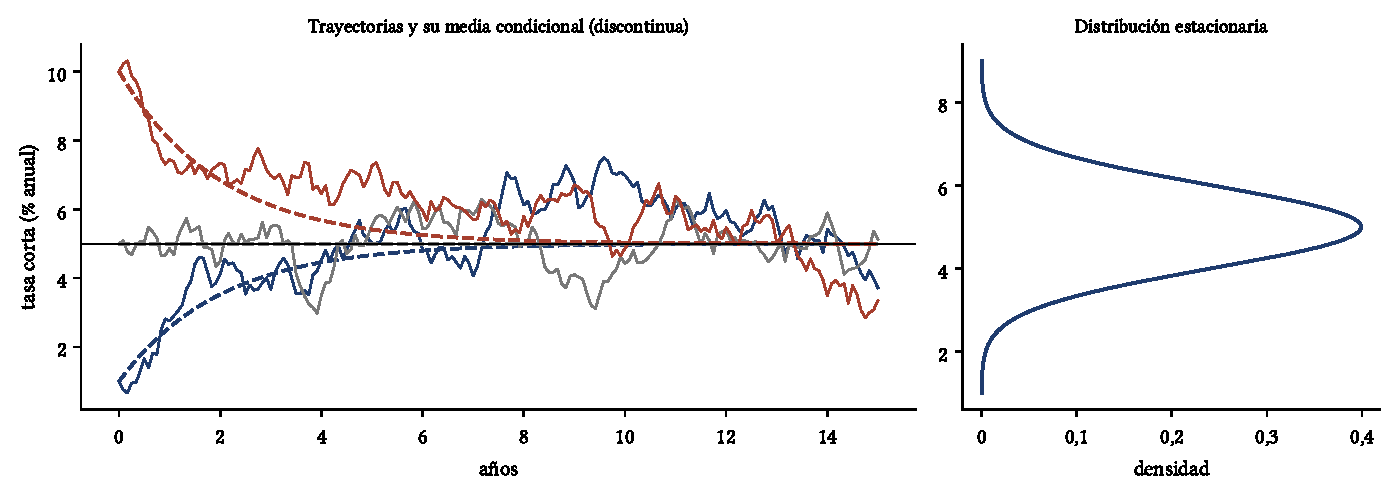
\includegraphics[width=\linewidth]{graficos/cap15_fig_vasicek.pdf}
\caption{Modelo de Vasicek con $\kappa=0{,}5$, $\theta=5$ y $\sigma=1$, simulado mes a mes con la discretización exacta.
Izquierda: tres trayectorias y su media condicional $\theta+(r_0-\theta)e^{-\kappa t}$. Derecha: distribución estacionaria
$N(5;\,1)$, que asigna una probabilidad positiva a tasas negativas.}
\label{fig:vasicek}
\end{figure}

\paragraph{El modelo CKLS.} En Vasicek la volatilidad no depende del nivel, y la tasa puede volverse negativa. Chan,
Karolyi, Longstaff y Sanders (1992) anidan varios modelos en
\[
  dr_t=(\alpha+\beta r_t)\,dt+\sigma\,r_t^{\gamma}\,dW_t ,
\]
donde $\gamma=0$ es Vasicek, $\gamma=1/2$ es Cox, Ingersoll y Ross (1985) y $\gamma=1$ es un movimiento browniano
geométrico con reversión. Con un paso pequeño, $\Var(\varepsilon_{t+\Delta}\mid r_t)\approx\sigma^2r_t^{2\gamma}\Delta$, de modo que
\[
  \ln\varepsilon_{t+\Delta}^2\approx\ln(\sigma^2\Delta)+2\gamma\ln r_t+\ln\eta^2_{t+\Delta},
\]
con $\eta$ normal estándar. Una regresión del logaritmo del residuo al cuadrado sobre el logaritmo del nivel estima $2\gamma$
de forma simple. CKLS estimaron $\gamma\approx1{,}5$ por MGM con la tasa a un mes de 1964 a 1989.

% ---------------------------------------------------------------------
\section{Ejercicios resueltos}
% ---------------------------------------------------------------------

\begin{ejresuelto}{Hechos estilizados de la curva}\label{ej:curva}
\enunciado Describa los diez rendimientos: medias, volatilidades, persistencia y correlaciones. Calcule la pendiente
$y_{120}-y_3$ y cuente los meses con curva invertida. Extraiga los componentes principales de la matriz de covarianzas e
interprételos.

\solucion
\paso{Paso 1. Estadísticas descriptivas.}
\begin{center}\small
\begin{tabular}{@{}rrrrrr@{}}
\toprule
Vencimiento (meses) & Media & Desv.\ est. & $\hat\rho(1)$ & $\hat\rho(12)$ & Corr.\ con 1 mes \\
\midrule
1   & 4,820 & 3,193 & 0,9800 & 0,8260 & 1,0000 \\
3   & 5,126 & 3,285 & 0,9844 & 0,8382 & 0,9963 \\
12  & 5,526 & 3,354 & 0,9862 & 0,8617 & 0,9853 \\
36  & 5,821 & 3,302 & 0,9900 & 0,8935 & 0,9624 \\
60  & 5,973 & 3,267 & 0,9918 & 0,9056 & 0,9492 \\
120 & 6,157 & 3,188 & 0,9937 & 0,9204 & 0,9329 \\
\bottomrule
\end{tabular}
\end{center}
La curva \emph{media} sube: de 4,82\,\% a un mes a 6,16\,\% a diez años. La volatilidad casi no cambia con el plazo. Todos
los rendimientos son muy persistentes (autocorrelación mensual de 0,98 a 0,99, más alta cuanto más largo el plazo) y están
muy correlacionados entre sí, aunque la correlación cae con la distancia entre vencimientos.

\paso{Paso 2. La pendiente.} La pendiente $y_{120}-y_3$ tiene una media de $1{,}032$ puntos porcentuales. La curva estuvo
invertida en 63 de 531 meses (11,9\,\%). El mínimo, $-3{,}223$, ocurrió en marzo de 1980, durante el endurecimiento monetario
de Volcker; el máximo, $4{,}108$, en agosto de 1982, cuando la política se relajó y las tasas cortas cayeron primero.

\paso{Paso 3. Componentes principales.} Los tres primeros explican el 98,25\,\%, el 1,54\,\% y el 0,15\,\% de la varianza
total (99,94\,\% en conjunto). Sus cargas:
\begin{center}\small
\begin{tabular}{@{}rrrr@{}}
\toprule
Vencimiento & CP1 & CP2 & CP3 \\
\midrule
1   & 0,306 & $-0{,}316$ & 0,527 \\
3   & 0,317 & $-0{,}267$ & 0,148 \\
6   & 0,323 & $-0{,}184$ & $-0{,}239$ \\
12  & 0,325 & $-0{,}019$ & $-0{,}423$ \\
36  & 0,318 & 0,334 & $-0{,}146$ \\
60  & 0,312 & 0,464 & 0,073 \\
120 & 0,300 & 0,576 & 0,374 \\
\bottomrule
\end{tabular}
\end{center}
El primero carga casi igual en todos los plazos (0,30 a 0,325): mueve toda la curva en paralelo, es el \emph{nivel}. El
segundo crece de forma monótona con el plazo, de $-0{,}316$ a $0{,}576$: inclina la curva, es la \emph{pendiente}. El
tercero es positivo en los extremos y negativo en los plazos de 6 a 36 meses: dobla la curva, es la \emph{curvatura}. Es el
patrón de Litterman y Scheinkman (Figura~\ref{fig:curvas}).

\codigoweb{cap15_ej01}
\salidaR{cap15_ej01_R.txt}
\lectura{cap15_ej01}

\RvsPy El signo de los autovectores es arbitrario y \texttt{eigen} (R) y \texttt{np.linalg.eigh} (Python) no siempre coinciden.
Fijamos cada signo para que la carga a 120 meses sea positiva. \texttt{eigh} devuelve los autovalores de menor a mayor, así
que en Python se invierte el orden. Las autocorrelaciones salen de \texttt{acf} en R y de
\texttt{statsmodels.tsa.stattools.acf} en Python, que usan la misma definición (sumas centradas divididas entre la suma
total de cuadrados).

\begin{figure}[ht]
\centering
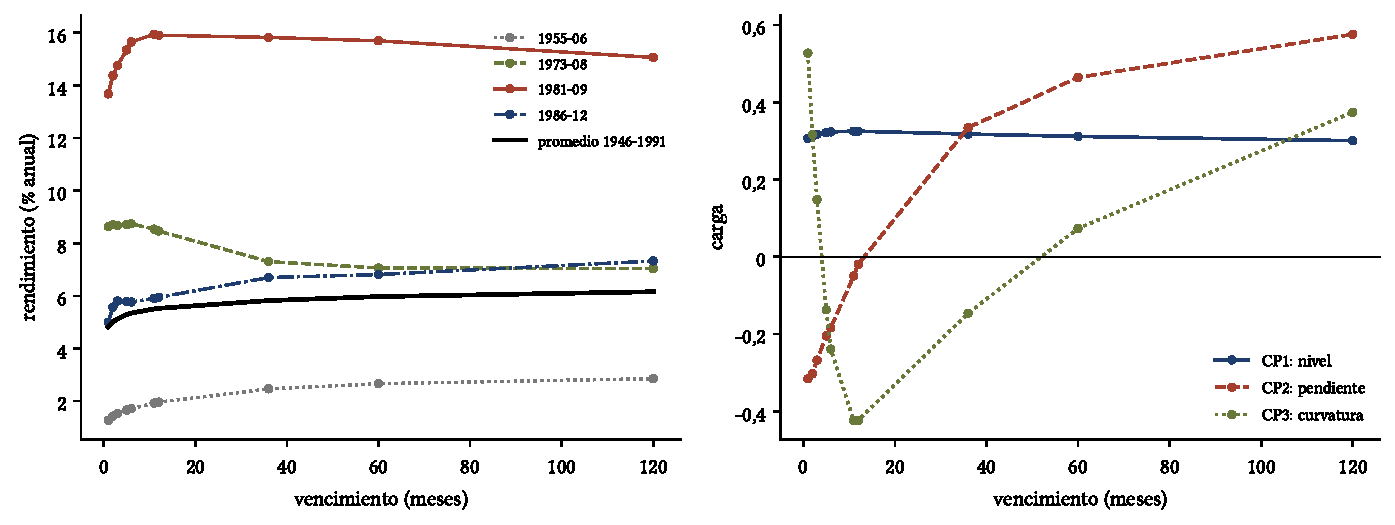
\includegraphics[width=\linewidth]{graficos/cap15_ej01_curvas_cp.pdf}
\caption{Izquierda: curvas observadas en cuatro fechas y la curva media de 1946 a 1991. En septiembre de 1981 la curva tiene joroba:
sube de 13,7\,\% a un mes a 15,9\,\% a 11 meses y baja a 15,1\,\% a diez años. Derecha: cargas de los tres primeros componentes principales: nivel, pendiente y curvatura.}
\label{fig:curvas}
\end{figure}

\begin{conclusion}
La curva de rendimientos es, en la práctica, un objeto de tres dimensiones. El nivel explica casi toda la varianza, pero la
pendiente y la curvatura, aunque pequeñas, son las que contienen información sobre expectativas y primas por plazo.
\end{conclusion}
\end{ejresuelto}

\begin{ejresuelto}{La hipótesis de las expectativas}\label{ej:he}
\enunciado Contraste la HE con (a) la regresión de tasas cortas futuras de la Proposición~\ref{prop:he1}, para
$(m,k)=(1,3),(1,6),(1,12)$ con datos mensuales y $(12,36),(12,60),(12,120)$ renovando bonos de un año, con errores de
Newey-West de $k$ rezagos; y (b) la regresión de la tasa larga de la Proposición~\ref{prop:he2} con $n=12$ meses.

\solucion
\paso{Paso 1. Tasas cortas futuras.} Para $(m,k)=(1,3)$, el lado izquierdo es el promedio de la tasa a un mes en
$t$, $t+1$ y $t+2$ menos la tasa de hoy, y el regresor es $y_{3,t}-y_{1,t}$. Se pierden $k-m=2$ observaciones al final.
\begin{center}\small
\begin{tabular}{@{}rrrrrrr@{}}
\toprule
$m$ & $k$ & $n$ & $\hat b$ & ee($\hat b$) & $t(b=1)$ & $R^2$ \\
\midrule
1  & 3   & 529 & 0,4447 & 0,1381 & $-4{,}02$ & 0,082 \\
1  & 6   & 526 & 0,2928 & 0,1429 & $-4{,}95$ & 0,030 \\
1  & 12  & 520 & 0,2468 & 0,1738 & $-4{,}33$ & 0,022 \\
12 & 36  & 507 & 0,2000 & 0,3928 & $-2{,}04$ & 0,007 \\
12 & 60  & 483 & 0,5566 & 0,3969 & $-1{,}12$ & 0,061 \\
12 & 120 & 423 & 1,5406 & 0,2580 & 2,10 & 0,519 \\
\bottomrule
\end{tabular}
\end{center}
Para $(1,3)$, el estadístico es
\begin{align*}
  t &= \frac{0{,}4447-1}{0{,}1381}\\
    &= \frac{-0{,}5553}{0{,}1381}\\
    &= -4{,}02 .
\end{align*}
En el extremo corto los coeficientes son positivos, la pendiente sí predice la dirección de las tasas, pero muy por
debajo de uno: la HE se rechaza con claridad. A horizontes largos el coeficiente sube y a diez años supera a uno, el patrón
en forma de U que documentaron Campbell y Shiller (1991). Con 423 observaciones solapadas a diez años hay pocas
observaciones independientes y el resultado debe leerse con cautela.

\paso{Paso 2. La tasa larga.} Con $n=12$, el lado izquierdo es $y_{11,t+1}-y_{12,t}$ y el regresor $(y_{12,t}-y_{1,t})/11$:
\begin{align*}
  \hat b &= -1{,}3515 \quad(\text{ee }0{,}6210),\\
  t(b=1) &= \frac{-1{,}3515-1}{0{,}6210}\\
         &= \frac{-2{,}3515}{0{,}6210}\\
         &= -3{,}79 .
\end{align*}
El coeficiente no solo es menor que uno: es \emph{negativo}. Cuando la curva sube, el rendimiento a un año tiende a bajar en
el mes siguiente, lo contrario de lo que exige la HE (Figura~\ref{fig:he}).

\codigoweb{cap15_ej02}
\salidaR{cap15_ej02_R.txt}
\lectura{cap15_ej02}

\RvsPy La función \texttt{mco\_nw} es nuestra en ambos lenguajes, para controlar el núcleo de Bartlett y el número de
rezagos. En Python, la opción \texttt{cov\_type="HAC"} de \texttt{statsmodels}, con
\texttt{cov\_kwds=\{"maxlags": k\}}, da los mismos errores (lo comprobamos en la regresión de la tasa larga: 0,6210). En R,
la función \texttt{NeweyWest} del paquete \texttt{sandwich}, con \texttt{prewhite = FALSE} y \texttt{adjust = FALSE}, usa
los mismos pesos. El
promedio de las tasas futuras se arma con índices $t+m\,i$; en R conviene \texttt{sapply}, en Python una comprensión de listas.

\begin{figure}[ht]
\centering
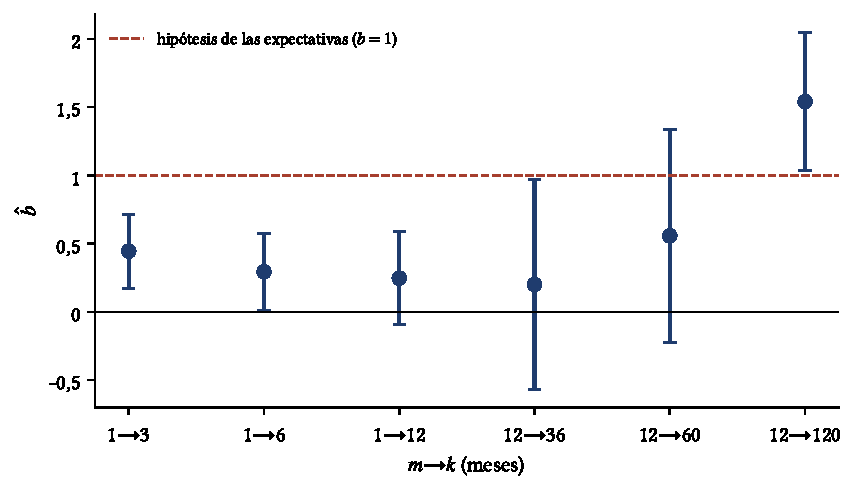
\includegraphics[width=0.8\linewidth]{graficos/cap15_ej02_expectativas.pdf}
\caption{Coeficientes de la regresión de tasas cortas futuras con intervalos al 95\,\% (Newey-West). La HE exige que todos
estén en la línea discontinua.}
\label{fig:he}
\end{figure}

\begin{conclusion}
La pendiente de la curva predice las tasas futuras en la dirección correcta, pero mucho menos de lo que exige la HE en el
corto plazo, y la tasa larga se mueve en sentido contrario. La explicación más aceptada es una prima por plazo que varía
en el tiempo y que hace que la pendiente mida, en parte, esa prima y no solo expectativas.
\end{conclusion}
\end{ejresuelto}

\begin{ejresuelto}{Rendimientos en exceso y Fama-Bliss}\label{ej:fb}
\enunciado Calcule los rendimientos en exceso a un mes de los bonos de 2, 3, 6 y 12 meses, sus medias y razones de Sharpe, y
estime la regresión de Fama y Bliss sobre el diferencial a plazo.

\solucion
\paso{Paso 1. Unidades.} Los rendimientos están en porcentaje anual y el período es un mes, así que la tasa por período es
$y/12$. Por la definición y la Proposición~\ref{prop:plazo}, en porcentaje mensual,
\begin{align*}
  rx_{t+1}(n) &= \frac{n}{12}\,y_{n,t}-\frac{n-1}{12}\,y_{n-1,t+1}-\frac{y_{1,t}}{12},\\
  \frac{f_t(n)-y_{1,t}}{12} &= \frac{n\,y_{n,t}-(n-1)\,y_{n-1,t}-y_{1,t}}{12}.
\end{align*}
Los vencimientos disponibles permiten $n-1=1,2,5,11$ para $n=2,3,6,12$.

\paso{Paso 2. Resultados.}
\begin{center}\small
\begin{tabular}{@{}rrrrrrrr@{}}
\toprule
$n$ & Media $rx$ & Desv.\ est. & Sharpe anual & $\hat b$ & ee & $t(b=0)$ & $R^2$ \\
\midrule
2  & 0,0302 & 0,0509 & 2,053 & 0,5159 & 0,0990 & 5,21 & 0,118 \\
3  & 0,0435 & 0,0964 & 1,563 & 0,6973 & 0,1958 & 3,56 & 0,091 \\
6  & 0,0641 & 0,2324 & 0,956 & 1,3023 & 0,3297 & 3,95 & 0,103 \\
12 & 0,0689 & 0,4882 & 0,489 & 1,1656 & 0,4836 & 2,41 & 0,035 \\
\bottomrule
\end{tabular}
\end{center}
Los bonos más largos rinden más en promedio: el de 12 meses rinde $0{,}0689\times12=0{,}83$ puntos porcentuales anuales más
que la letra a un mes. Pero su volatilidad crece más rápido, por el factor de duración $(n-1)$ de la
Proposición~\ref{prop:rx}, y la razón de Sharpe cae de 2,05 a 0,49.

\paso{Paso 3. Fama-Bliss.} Bajo la HE, $b=0$. Para $n=2$:
\begin{align*}
  t &= \frac{0{,}5159-0}{0{,}0990}\\
    &= 5{,}21 .
\end{align*}
Los cuatro coeficientes son positivos y significativos; para 6 y 12 meses son cercanos a uno, lo que significa que un
punto más de diferencial a plazo se traduce casi uno a uno en un punto más de rendimiento en exceso esperado, y nada en
cambio de la tasa futura. El $R^2$ es bajo (de 3,5 a 11,8\,\%): la prima predecible es pequeña frente al ruido mensual, pero
existe (Figura~\ref{fig:fb}).

\codigoweb{cap15_ej03}
\salidaR{cap15_ej03_R.txt}
\lectura{cap15_ej03}

\RvsPy Los rendimientos en exceso combinan una columna en $t$ con otra en $t+1$. En R, \texttt{x[-T]} quita la última
observación y \texttt{x[-1]} la primera; en Python, \texttt{x[:-1]} y \texttt{x[1:]}. Es el error más común en este tipo de
cálculo: desalinear las fechas produce coeficientes que parecen razonables y son falsos.

\begin{figure}[ht]
\centering
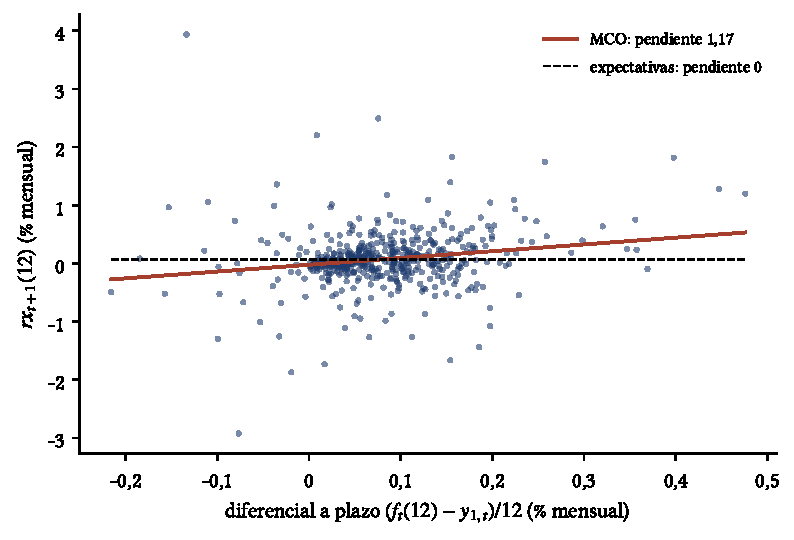
\includegraphics[width=0.75\linewidth]{graficos/cap15_ej03_fama_bliss.pdf}
\caption{Rendimiento en exceso del bono de 12 meses frente al diferencial a plazo en el mes anterior, con la recta de MCO y la
predicción de la HE (pendiente cero).}
\label{fig:fb}
\end{figure}

\begin{conclusion}
Comprar bonos cuando la tasa a plazo está alta respecto de la tasa corta fue, en promedio, rentable. Es la otra cara del
rechazo de la HE en el Ejercicio~\ref{ej:he}: la tasa a plazo contiene una prima de riesgo que varía en el tiempo, no solo
el pronóstico de la tasa futura.
\end{conclusion}
\end{ejresuelto}

\begin{ejresuelto}{Nelson-Siegel dinámico}\label{ej:ns}
\enunciado Ajuste el modelo de Nelson-Siegel mes a mes por MCO de corte transversal: (a) con el $\lambda$ que minimiza la suma
total de errores cuadráticos en una malla de 0,010 a 0,200 con paso 0,0005, y (b) con $\lambda=0{,}0609$. Compare el ajuste, la
persistencia de los factores y su relación con el nivel, la pendiente y la curvatura empíricos.

\solucion
\paso{Paso 1. El parámetro $\lambda$.} El mínimo de la malla está en $\hat\lambda=0{,}1410$, que pone el máximo de la curvatura en
\begin{align*}
  \tau^* &= \frac{1{,}7933}{0{,}1410}\\
         &= 12{,}7\ \text{meses}.
\end{align*}
Con estos datos, cuyos plazos se concentran por debajo del año, el ajuste prefiere una joroba más temprana que la de
Diebold y Li (Figura~\ref{fig:nslambda}).

\paso{Paso 2. Ajuste y factores.}
\begin{center}\small
\begin{tabular}{@{}lrrrrrr@{}}
\toprule
 & \multicolumn{3}{c}{$\lambda=0{,}1410$} & \multicolumn{3}{c}{$\lambda=0{,}0609$} \\
\cmidrule(lr){2-4}\cmidrule(lr){5-7}
 & Media & $\hat\rho(1)$ & $\hat\rho(12)$ & Media & $\hat\rho(1)$ & $\hat\rho(12)$ \\
\midrule
$\hat\beta_0$ & 6,134 & 0,994 & 0,921 & 6,098 & 0,993 & 0,928 \\
$\hat\beta_1$ & $-1{,}328$ & 0,902 & 0,346 & $-1{,}190$ & 0,923 & 0,393 \\
$\hat\beta_2$ & 0,210 & 0,807 & 0,408 & 1,061 & 0,758 & 0,315 \\
\midrule
RECM global & \multicolumn{3}{c}{0,102} & \multicolumn{3}{c}{0,130} \\
\bottomrule
\end{tabular}
\end{center}
Tres parámetros por mes ajustan diez rendimientos con un error cuadrático medio de 10 a 13 puntos básicos. Los mayores
errores con $\lambda=0{,}0609$ están en el plazo de un mes (0,237) y en el de 36 meses (0,164). El nivel es casi tan persistente
como los propios rendimientos; la pendiente y la curvatura lo son menos, pero aun así mucho (autocorrelación mensual de 0,76 a 0,92).

\paso{Paso 3. Interpretación.} Con $\lambda=0{,}0609$:
\begin{align*}
  \operatorname{corr}(\hat\beta_0,\ y_{120}) &= 0{,}991,\\
  \operatorname{corr}(-\hat\beta_1,\ y_{120}-y_3) &= 0{,}984,\\
  \operatorname{corr}(\hat\beta_2,\ 2y_{36}-y_3-y_{120}) &= 0{,}702 .
\end{align*}
Los factores tienen exactamente la interpretación de la Proposición~\ref{prop:ns} (Figura~\ref{fig:nsfac}). La curvatura es
la peor medida por su proxy empírico, que usa solo tres plazos. En septiembre de 1981, cuando la curva subía hasta 15,9\,\% a 11 meses y bajaba a 15,1\,\% a diez años,
$\hat\beta_1=0{,}420$ es positivo (el tramo largo queda por debajo del corto) y $\hat\beta_2=8{,}597$ refleja una joroba pronunciada; la RECM de ese mes, 0,314, es la mayor de las tres fechas
de la Figura~\ref{fig:nsajuste}.

\codigoweb{cap15_ej04}
\salidaR{cap15_ej04_R.txt}
\lectura{cap15_ej04}

\RvsPy Con $\lambda$ fijo, las 531 regresiones de corte transversal se resuelven con un solo sistema: $\hat B'=(X'X)^{-1}X'Y'$, donde
$X$ es la matriz $10\times3$ de cargas. En Python la malla se redondea (\texttt{np.round(..., 4)}) porque \texttt{np.arange} con
paso decimal acumula errores de punto flotante y el mínimo podría imprimirse como 0,14099999. En R, \texttt{seq} no tiene
ese problema en esta escala.

\begin{figure}[ht]
\centering
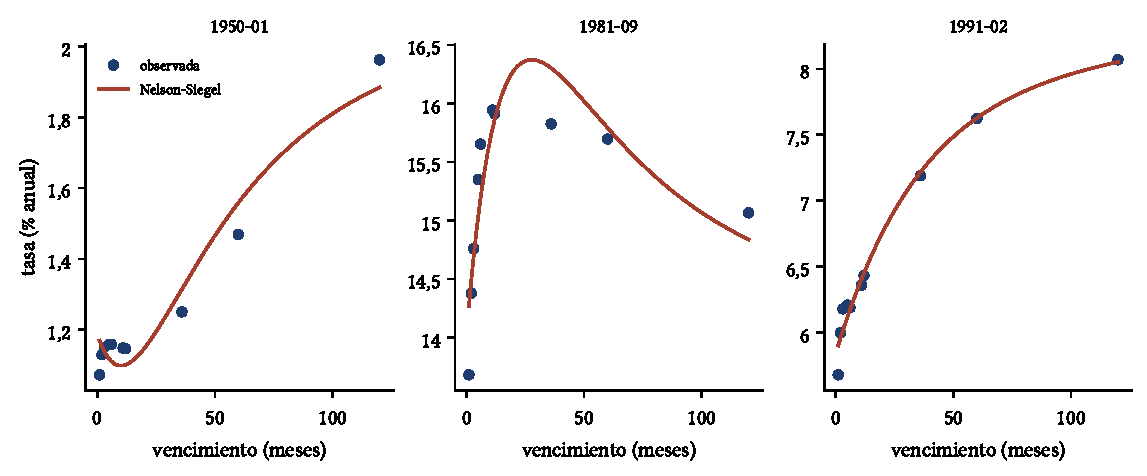
\includegraphics[width=\linewidth]{graficos/cap15_ej04_ajustes.pdf}
\caption{Curvas observadas (puntos) y ajustadas por Nelson-Siegel con $\lambda=0{,}0609$ en tres fechas: una curva baja y
creciente (1950), una con joroba y tramo largo descendente (1981) y una creciente al final de la muestra (1991).}
\label{fig:nsajuste}
\end{figure}

\begin{figure}[ht]
\centering
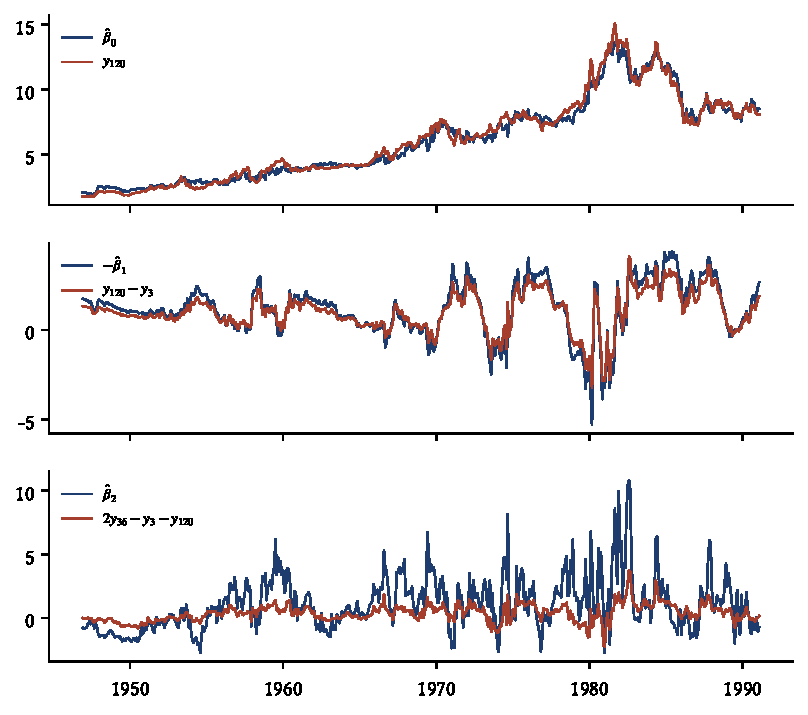
\includegraphics[width=0.85\linewidth]{graficos/cap15_ej04_factores.pdf}
\caption{Factores de Nelson-Siegel estimados (azul) y sus contrapartes empíricas (rojo): nivel, pendiente y curvatura.}
\label{fig:nsfac}
\end{figure}

\begin{figure}[ht]
\centering
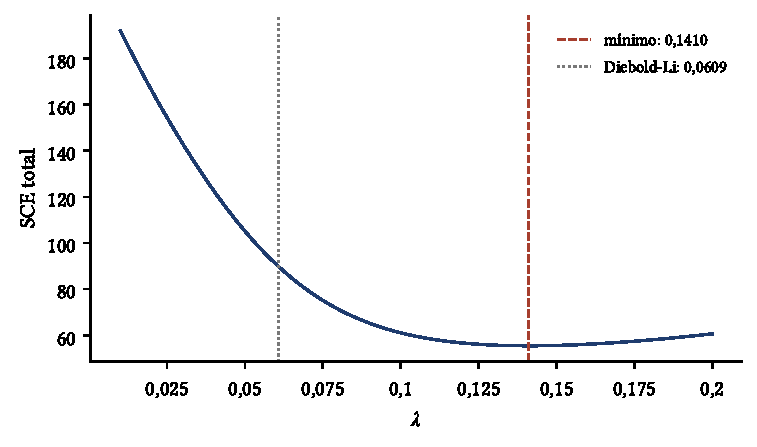
\includegraphics[width=0.7\linewidth]{graficos/cap15_ej04_lambda.pdf}
\caption{Suma de errores cuadráticos de todos los meses y vencimientos en función de $\lambda$.}
\label{fig:nslambda}
\end{figure}

\begin{conclusion}
El modelo de Nelson-Siegel dinámico logra con tres factores interpretables casi el mismo ajuste que los componentes
principales, pero con cargas suaves que permiten interpolar a cualquier plazo. Su $\lambda$ óptimo depende de los vencimientos
disponibles; fijarlo en 0,0609 cuesta poco en ajuste y facilita comparar con la literatura.
\end{conclusion}
\end{ejresuelto}

\begin{ejresuelto}{Vasicek y el efecto nivel}\label{ej:vasicek}
\enunciado Estime el modelo de Vasicek para la tasa a un mes con el AR(1) del Corolario~\ref{cor:vasicek} ($\Delta=1/12$
años). Calcule la vida media y la probabilidad estacionaria de tasas negativas. Luego contraste si la volatilidad depende
del nivel con la regresión de CKLS.

\solucion
\paso{Paso 1. El AR(1).} Por MCO, con $n=530$:
\[
  \hat a=0{,}10569\ (0{,}04752),\qquad \hat b=0{,}98016\ (0{,}00822),\qquad \hat s=0{,}60426 .
\]

\paso{Paso 2. Parámetros de Vasicek.}
\begin{align*}
  \hat\kappa &= -12\,\ln 0{,}98016\\
             &= -12\times(-0{,}020039)\\
             &= 0{,}2405\ \text{por año},\\[4pt]
  \hat\theta &= \frac{0{,}10569}{1-0{,}98016}\\
             &= \frac{0{,}10569}{0{,}01984}\\
             &= 5{,}327\text{\,\%},\\[4pt]
  1-\hat b^2 &= 1-0{,}960714\\
             &= 0{,}039286,\\
  \hat\sigma &= 0{,}60426\sqrt{\frac{2\times0{,}2405}{0{,}039286}}\\
             &= 0{,}60426\sqrt{12{,}243}\\
             &= 0{,}60426\times3{,}4991\\
             &= 2{,}114\text{\,\%}\ \text{por }\sqrt{\text{año}} .
\end{align*}
La vida media y la desviación estándar estacionaria son
\begin{align*}
  \frac{\ln2}{\hat\kappa} &= \frac{0{,}6931}{0{,}2405}\\
                          &= 2{,}88\ \text{años},\\[4pt]
  \frac{\hat\sigma}{\sqrt{2\hat\kappa}} &= \frac{2{,}114}{\sqrt{0{,}4809}}\\
                                         &= \frac{2{,}114}{0{,}6935}\\
                                         &= 3{,}049\text{\,\%}.
\end{align*}
La desviación estándar implícita (3,05) es parecida a la muestral (3,19), pero la media de largo plazo (5,33) está por encima
de la muestral (4,82): con una raíz tan cerca de uno, $\hat\theta$ es muy imprecisa. La probabilidad estacionaria de una tasa
negativa es $\Phi(-5{,}327/3{,}049)=0{,}040$, una de cada 25 observaciones, algo que nunca ocurrió en estos 44 años.

\paso{Paso 3. Efecto nivel.} La regresión de $\ln\hat e_t^2$ sobre $\ln r_{t-1}$ da
\begin{align*}
  2\hat\gamma &= 1{,}2787\ (0{,}1260)\\
  \hat\gamma  &= 0{,}639,\\
  t(\gamma=\tfrac12) &= \frac{1{,}2787-1}{0{,}1260}\\
                     &= 2{,}21 .
\end{align*}
Se rechaza $\gamma=0$ (Vasicek) con $t=10{,}15$, y también $\gamma=1/2$ (CIR) al 5\,\%. La desviación estándar de los residuos
lo muestra sin regresión: 0,273 cuando la tasa está en su tercil bajo (media 1,6\,\%), 0,330 en el medio (4,4\,\%) y 0,953 en el
alto (8,5\,\%) (Figura~\ref{fig:vasicekdatos}).

\codigoweb{cap15_ej05}
\salidaR{cap15_ej05_R.txt}
\lectura{cap15_ej05}

\RvsPy En R, \texttt{lm} entrega directamente los errores estándar; en Python escribimos la función \texttt{mco} con
$s^2(X'X)^{-1}$ para no depender de \texttt{statsmodels}. Los terciles se forman con \texttt{quantile} y
\texttt{np.quantile}, que usan
por omisión la misma interpolación (tipo 7), por eso los tamaños de los grupos (178, 175 y 177, desiguales por empates)
coinciden.

\begin{figure}[ht]
\centering
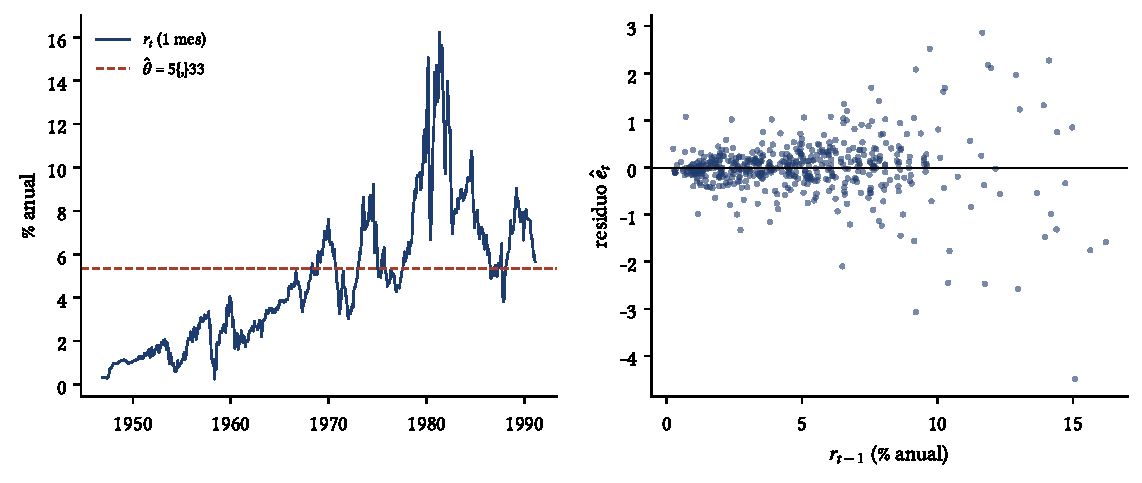
\includegraphics[width=\linewidth]{graficos/cap15_ej05_vasicek.pdf}
\caption{Izquierda: tasa a un mes y la media de largo plazo estimada por Vasicek. Derecha: residuos del AR(1) frente al
nivel del mes anterior; su dispersión crece con el nivel, en contra del supuesto de Vasicek.}
\label{fig:vasicekdatos}
\end{figure}

\begin{conclusion}
El modelo de Vasicek captura la reversión lenta de la tasa corta, pero su supuesto de volatilidad constante no se cumple: la
volatilidad crece con el nivel, con un exponente entre el de CIR y el de un proceso proporcional. Las conclusiones dependen
de la década de alta inflación y del experimento monetario de 1979--1982, como advierten CKLS.
\end{conclusion}
\end{ejresuelto}

% ---------------------------------------------------------------------
\section{Ejercicios propuestos}
% ---------------------------------------------------------------------

\begin{enumerate}[label=\textbf{\thechapter.\arabic*},leftmargin=*,itemsep=6pt]
  \item Con rendimientos compuestos en forma continua de 4\,\% a un año y 5\,\% a dos años, calcule la tasa a plazo entre el año
  1 y el 2, y el precio del bono cupón cero a cinco años si su rendimiento es 6\,\%. \textit{Respuesta: 6\,\%; $e^{-0{,}30}=0{,}7408$.}

  \item Con $\lambda=0{,}0609$ y $\boldsymbol\beta=(6;\,-2;\,1)$, calcule el rendimiento de Nelson-Siegel a 60 meses.
  \textit{Respuesta: las cargas son 0,2666 y 0,2407; $y(60)=5{,}708$\,\%.}

  \item Un AR(1) mensual de la tasa corta da $\hat a=0{,}15$, $\hat b=0{,}97$ y $\hat s=0{,}5$. Calcule $\kappa$, $\theta$, $\sigma$ y la
  vida media de Vasicek. \textit{Respuesta: $\kappa=0{,}3655$; $\theta=5$; $\sigma=1{,}758$; vida media $1{,}90$ años.}

  \item Demuestre que $y_{n,t}=\frac1n\sum_{i=1}^n f_t(i)$ y que, si la curva es creciente en $n$, entonces $f_t(n)\ge y_{n,t}$.

  \item Demuestre que, bajo la HE, la regresión de Fama y Bliss del cambio de la tasa corta,
  $y_{1,t+n-1}-y_{1,t}=a+b\,[f_t(n)-y_{1,t}]+u$, tiene $b=1$ cuando $n=2$.

  \item \emph{(Simulación.)} Simule 2\,000 muestras de 531 meses de un modelo de Vasicek con $\kappa=0{,}24$, $\theta=5{,}3$ y
  $\sigma=2{,}1$, y estime $\kappa$ en cada una con el Corolario~\ref{cor:vasicek}. ¿Cuál es el sesgo medio de $\hat\kappa$? Relaciónelo
  con el sesgo de Hurwicz de $\hat b$ (Capítulo~\ref{cap:raiz}).

  \item \emph{(Con datos del BCRP.)} Descargue de BCRPData los rendimientos de los bonos soberanos peruanos en soles en los
  plazos publicados (por ejemplo, 2, 5, 10, 15 y 20 años) y repita los Ejercicios~\ref{ej:curva} y \ref{ej:ns}. ¿Es el valor de $\lambda$ óptimo distinto del de Estados
  Unidos? ¿Por qué cabe esperarlo, si los plazos disponibles son otros?

  \item \emph{(Con datos.)} Repita el Ejercicio~\ref{ej:he} con dos submuestras: hasta septiembre de 1979 y desde octubre de 1979. ¿Se
  sostienen los resultados fuera del período de Volcker?
\end{enumerate}

% ---------------------------------------------------------------------
\section{Resumen de fórmulas}
% ---------------------------------------------------------------------

\begin{table}[H]
\centering\small
\begin{tabular}{@{}ll@{}}
\toprule
Concepto & Fórmula \\
\midrule
Precio y rendimiento & $P_{n,t}=e^{-n\,y_{n,t}}$;\quad $p_{n,t}=-n\,y_{n,t}$ \\
Tasa a plazo & $f_t(n,m)=\frac{m\,y_{m,t}-n\,y_{n,t}}{m-n}$;\quad $f_t(n)=n\,y_{n,t}-(n-1)\,y_{n-1,t}$ \\
Rendimiento en exceso & $rx_{t+1}(n)=[f_t(n)-y_{1,t}]-(n-1)[y_{n-1,t+1}-y_{n-1,t}]$ \\
HE: tasas cortas & $\frac1h\sum_{i=0}^{h-1}y_{m,t+mi}-y_{m,t}=a+b(y_{k,t}-y_{m,t})$;\quad $b=1$ \\
HE: tasa larga & $y_{n-1,t+1}-y_{n,t}=a+b\,\frac{y_{n,t}-y_{1,t}}{n-1}$;\quad $b=1$ \\
Fama-Bliss & $rx_{t+1}(n)=a+b\,[f_t(n)-y_{1,t}]$;\quad $b=0$ \\
Nelson-Siegel & $y(\tau)=\beta_0+\beta_1\frac{1-e^{-\lambda\tau}}{\lambda\tau}+\beta_2\bigl(\frac{1-e^{-\lambda\tau}}{\lambda\tau}-e^{-\lambda\tau}\bigr)$ \\
Vasicek exacto & $r_{t+\Delta}=\theta+e^{-\kappa\Delta}(r_t-\theta)+\varepsilon$;\quad $\Var(\varepsilon)=\sigma^2\frac{1-e^{-2\kappa\Delta}}{2\kappa}$ \\
Del AR(1) a Vasicek & $\kappa=-\ln b/\Delta$;\quad $\theta=a/(1-b)$;\quad $\sigma=s\sqrt{2\kappa/(1-b^2)}$ \\
CKLS & $dr=(\alpha+\beta r)\,dt+\sigma r^{\gamma}dW$;\quad $\ln\hat e^2_t\approx c+2\gamma\ln r_{t-1}$ \\
\bottomrule
\end{tabular}
\caption{Fórmulas principales del Capítulo 15.}
\end{table}

\section*{Referencias}
\begin{itemize}[leftmargin=*]
  \item Campbell, J. Y. y Shiller, R. J. (1991). Yield spreads and interest rate movements: A bird's eye view. \emph{Review of
        Economic Studies}, 58(3), 495--514.
  \item Chan, K. C., Karolyi, G. A., Longstaff, F. A. y Sanders, A. B. (1992). An empirical comparison of alternative models of
        the short-term interest rate. \emph{Journal of Finance}, 47(3), 1209--1227.
  \item Christensen, J. H. E., Diebold, F. X. y Rudebusch, G. D. (2011). The affine arbitrage-free class of Nelson-Siegel term
        structure models. \emph{Journal of Econometrics}, 164(1), 4--20.
  \item Cox, J. C., Ingersoll, J. E. y Ross, S. A. (1985). A theory of the term structure of interest rates. \emph{Econometrica},
        53(2), 385--407.
  \item Diebold, F. X. y Li, C. (2006). Forecasting the term structure of government bond yields. \emph{Journal of
        Econometrics}, 130(2), 337--364.
  \item Fama, E. F. y Bliss, R. R. (1987). The information in long-maturity forward rates. \emph{American Economic Review},
        77(4), 680--692.
  \item Litterman, R. y Scheinkman, J. (1991). Common factors affecting bond returns. \emph{Journal of Fixed Income}, 1(1),
        54--61.
  \item McCulloch, J. H. y Kwon, H.-C. (1993). U.S. term structure data, 1947--1991. Documento de trabajo, Ohio State University.
  \item Nelson, C. R. y Siegel, A. F. (1987). Parsimonious modeling of yield curves. \emph{Journal of Business}, 60(4), 473--489.
  \item Vasicek, O. (1977). An equilibrium characterization of the term structure. \emph{Journal of Financial Economics}, 5(2),
        177--188.
\end{itemize}

% =====================================================================
%  Capítulo 16. Estudios de eventos
% =====================================================================
\chapter[Estudios de eventos]{Estudios de eventos: rendimientos anormales, pruebas y sus trampas}\label{cap:eventos}

\section*{Objetivos de aprendizaje}
Al terminar este capítulo, el lector podrá:
\begin{enumerate}[label=\arabic*.,leftmargin=*]
  \item Diseñar un estudio de eventos: fecha del evento, ventanas de estimación y del evento, y modelo de rendimiento
        normal.
  \item Calcular rendimientos anormales y acumulados con su varianza exacta, incluido el error de estimación, y
        demostrar su equivalencia con una regresión con variables ficticias.
  \item Agregar muchos eventos y aplicar las pruebas paramétricas ($J_1$, Patell, Boehmer-Musumeci-Poulsen) y no
        paramétricas (signo y rangos de Corrado).
  \item Reconocer las dos trampas más comunes, los eventos simultáneos y la varianza inducida por el evento, y medir
        con simulaciones el tamaño y la potencia de cada prueba.
\end{enumerate}

\section*{Motivación}
El 25 de julio de 2018, después del cierre, Facebook publicó sus resultados del segundo trimestre. Al día siguiente su
acción cayó cerca de 19\,\%, la mayor pérdida de valor de mercado de una empresa estadounidense en un solo día hasta ese
momento. ¿Cuánto de esa caída se debe al anuncio y cuánto al mercado? ¿Es estadísticamente distinta de un mal día
cualquiera? El estudio de eventos, formalizado por Fama, Fisher, Jensen y Roll (1969), responde estas preguntas comparando el
rendimiento observado con el que se habría esperado sin el evento. Es probablemente la herramienta empírica más usada
en finanzas corporativas, en derecho (para cuantificar daños en litigios de valores) y en la evaluación de políticas,
como los anuncios de un banco central.

\paragraph{Datos del capítulo.} Precios de cierre diarios ajustados de Apple (AAPL), Amazon (AMZN), Facebook (FB) y
Alphabet (GOOG), de enero de 2014 a diciembre de 2018, y el índice S\&P 500 en las mismas fechas (1\,257 rendimientos
diarios). Para los anuncios de política monetaria usamos el S\&P 500 desde 1999, el índice de volatilidad VIX y las 40
fechas de las reuniones programadas del Comité Federal de Mercado Abierto (FOMC) de 2014 a 2018, tomadas de las páginas
históricas de la Reserva Federal. Los rendimientos son simples y en porcentaje.

% ---------------------------------------------------------------------
\section{El diseño de un estudio de eventos}
% ---------------------------------------------------------------------

Un estudio de eventos mide el tiempo en días hábiles relativos al evento, $\tau$. El día 0 es el primer día en que el
mercado pudo reaccionar: si la noticia sale después del cierre, como los resultados de Facebook, el día 0 es el día
hábil siguiente. Se definen dos ventanas (Figura~\ref{fig:lineatiempo}):
\begin{itemize}[leftmargin=*]
  \item la \emph{ventana de estimación}, de $L_1$ días antes del evento, donde se estima cómo se comporta el activo en
        condiciones normales; en este capítulo, $\tau=-250,\dots,-11$, con $L_1=240$;
  \item la \emph{ventana del evento}, de $L_2$ días alrededor del día 0, donde se mide el efecto; aquí,
        $\tau=-5,\dots,+5$, con $L_2=11$.
\end{itemize}
El espacio entre ambas ($\tau=-10,\dots,-6$) evita que una filtración previa al anuncio contamine la estimación.

\begin{figure}[ht]
\centering
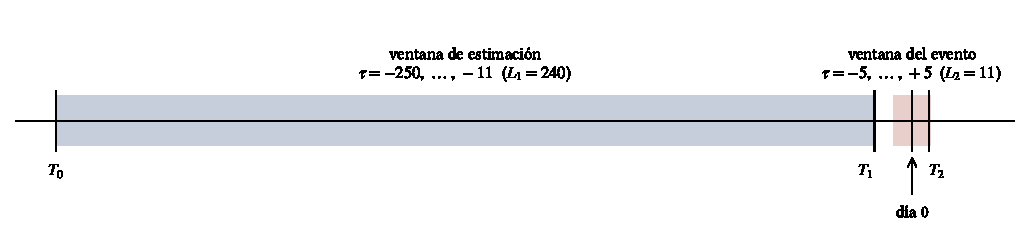
\includegraphics[width=\linewidth]{graficos/cap16_fig_linea_tiempo.pdf}
\caption{Línea de tiempo de un estudio de eventos con las ventanas usadas en el capítulo.}
\label{fig:lineatiempo}
\end{figure}

\begin{definicion}[Rendimiento anormal]
El rendimiento anormal del activo $i$ en el día $\tau$ es la diferencia entre el rendimiento observado y el rendimiento
normal estimado, $AR_{i\tau}=R_{i\tau}-\hat\E[R_{i\tau}\mid\text{sin evento}]$. El rendimiento anormal acumulado entre
$\tau_1$ y $\tau_2$ es $CAR_i(\tau_1,\tau_2)=\sum_{\tau=\tau_1}^{\tau_2}AR_{i\tau}$.
\end{definicion}

Los tres modelos de rendimiento normal más usados son:
\begin{itemize}[leftmargin=*]
  \item \textbf{media constante}: $R_{i\tau}=\mu_i+\varepsilon_{i\tau}$, de modo que $AR_{i\tau}=R_{i\tau}-\bar R_i$;
  \item \textbf{ajustado por mercado}: $AR_{i\tau}=R_{i\tau}-R_{m\tau}$, sin parámetros que estimar (equivale a fijar
        $\alpha=0$ y $\beta=1$);
  \item \textbf{modelo de mercado}: $R_{i\tau}=\alpha_i+\beta_iR_{m\tau}+\varepsilon_{i\tau}$, estimado por MCO en la
        ventana de estimación, de modo que $AR_{i\tau}=R_{i\tau}-\hat\alpha_i-\hat\beta_iR_{m\tau}$.
\end{itemize}
El modelo de mercado quita la parte del rendimiento que explica el mercado, lo que reduce la varianza del rendimiento
anormal tanto más cuanto mayor es el $R^2$ de la regresión. Pueden usarse modelos de factores (Capítulo~\ref{cap:factores}),
pero con datos diarios la ganancia sobre el modelo de mercado suele ser pequeña (MacKinlay, 1997).

% ---------------------------------------------------------------------
\section{La varianza de los rendimientos anormales}
% ---------------------------------------------------------------------

\begin{proposicion}[Varianza del rendimiento anormal]\label{prop:varar}
Sea el modelo de mercado con errores i.i.d.\ de varianza $\sigma^2$, independientes del mercado, estimado con $L_1$
observaciones. Sean $\hat\mu_m$ la media del mercado en la ventana de estimación y
$S_{mm}=\sum_{t}(R_{mt}-\hat\mu_m)^2$. Si no hay evento, condicionado en los rendimientos del mercado,
\[
  \E[AR_{i\tau}]=0,\qquad
  \Var(AR_{i\tau})=\sigma^2\Bigl[1+\frac1{L_1}+\frac{(R_{m\tau}-\hat\mu_m)^2}{S_{mm}}\Bigr].
\]
\end{proposicion}

\begin{proof}
Sin evento, $R_{i\tau}=\alpha_i+\beta_iR_{m\tau}+\varepsilon_{i\tau}$. Restamos el rendimiento normal estimado:
\begin{align*}
  AR_{i\tau} &= \alpha_i+\beta_iR_{m\tau}+\varepsilon_{i\tau}-\hat\alpha_i-\hat\beta_iR_{m\tau}\\
             &= \varepsilon_{i\tau}-\bigl[(\hat\alpha_i-\alpha_i)+(\hat\beta_i-\beta_i)R_{m\tau}\bigr].
\end{align*}
Los estimadores de MCO son insesgados, así que $\E[AR_{i\tau}]=0$. El término entre corchetes es el error de estimar la
recta en el punto $R_{m\tau}$. Depende solo de los errores de la ventana de estimación, que son independientes de
$\varepsilon_{i\tau}$; por tanto, las varianzas se suman. Escribiendo la recta en forma centrada,
$\hat\alpha_i+\hat\beta_ix=\bar R_i+\hat\beta_i(x-\hat\mu_m)$, donde $\bar R_i$ y $\hat\beta_i$ no están correlacionados:
\begin{align*}
  \Var(AR_{i\tau}) &= \Var(\varepsilon_{i\tau})+\Var\bigl(\bar R_i+\hat\beta_i(R_{m\tau}-\hat\mu_m)\bigr)\\
                   &= \sigma^2+\Var(\bar R_i)+(R_{m\tau}-\hat\mu_m)^2\Var(\hat\beta_i)\\
                   &= \sigma^2+\frac{\sigma^2}{L_1}+(R_{m\tau}-\hat\mu_m)^2\,\frac{\sigma^2}{S_{mm}}\\
                   &= \sigma^2\Bigl[1+\frac1{L_1}+\frac{(R_{m\tau}-\hat\mu_m)^2}{S_{mm}}\Bigr].
\end{align*}
\end{proof}

El primer término es la varianza del error del día del evento; los otros dos son el costo de no conocer $\alpha_i$ y
$\beta_i$. Con $L_1=240$ el segundo es $1/240=0{,}0042$, y el tercero es grande solo en días en que el mercado se movió mucho.
En forma matricial, si $X$ ($L_1\times2$) tiene las filas $(1,R_{mt})$ de la ventana de estimación y $X^*$ ($L_2\times2$) las
de la ventana del evento, el vector $\mathbf{AR}_i$ tiene covarianza
\[
  V_i=\sigma^2\bigl[I_{L_2}+X^*(X'X)^{-1}X^{*\prime}\bigr].
\]
Los elementos fuera de la diagonal no son cero: todos los $AR$ comparten el mismo error de estimación.

\begin{corolario}[Varianza del CAR]\label{cor:varcar}
Con $\boldsymbol\gamma$ el vector de unos en los días $\tau_1,\dots,\tau_2$ y ceros en el resto, $CAR_i=\boldsymbol\gamma'\mathbf{AR}_i$ y
\[
  \Var(CAR_i)=\boldsymbol\gamma'V_i\boldsymbol\gamma=\sigma^2\bigl[(\tau_2-\tau_1+1)+\boldsymbol\gamma'X^*(X'X)^{-1}X^{*\prime}\boldsymbol\gamma\bigr].
\]
\end{corolario}

\begin{proof}
Es la varianza de una combinación lineal:
\begin{align*}
  \Var(\boldsymbol\gamma'\mathbf{AR}_i) &= \boldsymbol\gamma'V_i\boldsymbol\gamma\\
                                        &= \sigma^2\boldsymbol\gamma'I\boldsymbol\gamma+\sigma^2\boldsymbol\gamma'X^*(X'X)^{-1}X^{*\prime}\boldsymbol\gamma\\
                                        &= \sigma^2(\tau_2-\tau_1+1)+\sigma^2\boldsymbol\gamma'X^*(X'X)^{-1}X^{*\prime}\boldsymbol\gamma,
\end{align*}
porque $\boldsymbol\gamma'\boldsymbol\gamma$ cuenta los unos de $\boldsymbol\gamma$.
\end{proof}

En la práctica se sustituye $\sigma^2$ por $s^2=\sum\hat\varepsilon_t^2/(L_1-2)$. Con errores normales, el cociente
$AR_{i\tau}/\sqrt{\hat V_{i,\tau\tau}}$ sigue una $t$ de Student con $L_1-2$ grados de libertad, y lo mismo el
$CAR$ estandarizado.

\begin{proposicion}[El rendimiento anormal como coeficiente de una ficticia]\label{prop:ficticia}
Agregue a la ventana de estimación la observación del día $\tau$ y estime por MCO
$R_{it}=\alpha_i+\beta_iR_{mt}+\delta\,D_t+u_t$, con $D_t=1$ solo en el día $\tau$. Entonces $\hat\delta=AR_{i\tau}$ y su error
estándar de MCO es exactamente $\sqrt{\hat V_{i,\tau\tau}}$ de la Proposición~\ref{prop:varar}.
\end{proposicion}

\begin{proof}
La ficticia solo actúa en el día $\tau$, así que $\hat\delta$ puede ajustar esa observación sin error y MCO lo hace: el
residuo del día $\tau$ es cero. Los demás residuos dependen solo de $(\hat\alpha_i,\hat\beta_i)$, que por tanto son los de la ventana
de estimación. Con $\mathbf x_\tau=(1,R_{m\tau})'$, la ecuación del día $\tau$ da
\begin{align*}
  R_{i\tau} &= \mathbf x_\tau'\hat{\mathbf b}+\hat\delta\\
  \hat\delta  &= R_{i\tau}-\mathbf x_\tau'\hat{\mathbf b}\\
             &= AR_{i\tau}.
\end{align*}
La suma de residuos al cuadrado es la de la ventana de estimación y los grados de libertad son $(L_1+1)-3=L_1-2$: la
estimación $s^2$ coincide. Falta el elemento de $(Z'Z)^{-1}$ que corresponde a $\delta$. Por la inversa de una matriz
particionada, es $1/(\mathbf d'M\mathbf d)$, donde $M$ es el aniquilador de las columnas $(1,R_m)$ en las $L_1+1$ observaciones.
Con $A=X'X$ de la ventana de estimación,
\begin{align*}
  \mathbf d'M\mathbf d &= 1-\mathbf x_\tau'(A+\mathbf x_\tau\mathbf x_\tau')^{-1}\mathbf x_\tau\\
                      &= 1-\mathbf x_\tau'\Bigl[A^{-1}-\frac{A^{-1}\mathbf x_\tau\mathbf x_\tau'A^{-1}}{1+\mathbf x_\tau'A^{-1}\mathbf x_\tau}\Bigr]\mathbf x_\tau\\
                      &= 1-q+\frac{q^2}{1+q}\\
                      &= \frac{(1-q)(1+q)+q^2}{1+q}\\
                      &= \frac{1}{1+q},
\end{align*}
donde $q=\mathbf x_\tau'A^{-1}\mathbf x_\tau$ y el segundo paso usa la fórmula de Sherman y Morrison. Entonces
\begin{align*}
  \widehat{\Var}(\hat\delta) &= \frac{s^2}{\mathbf d'M\mathbf d}\\
                           &= s^2(1+q)\\
                           &= s^2\bigl[1+\mathbf x_\tau'(X'X)^{-1}\mathbf x_\tau\bigr],
\end{align*}
que es el elemento diagonal de $\hat V_i$.
\end{proof}

La proposición dice que un estudio de eventos de un activo es una regresión con una ficticia por cada día del evento.
Esto permite usar todo el instrumental de la regresión: errores robustos, varios activos a la vez y pruebas conjuntas.

% ---------------------------------------------------------------------
\section{Agregación de eventos y pruebas}
% ---------------------------------------------------------------------

Un solo evento rara vez basta para sacar conclusiones generales: ¿afectan los anuncios de recompra de acciones al
precio? Se necesitan $N$ eventos. Sean $AR_i$ los rendimientos anormales del día de interés, $\hat\sigma_i^2$ sus varianzas
estimadas y $SAR_i=AR_i/\hat\sigma_i$ los rendimientos estandarizados. El rendimiento anormal medio es
$\overline{AR}=\frac1N\sum_iAR_i$ (o $CAAR$ si se acumula en una ventana). Si los eventos son independientes:
\begin{itemize}[leftmargin=*]
  \item \textbf{$J_1$} (Campbell, Lo y MacKinlay, 1997): $J_1=\overline{AR}\big/\sqrt{\sum_i\hat\sigma_i^2/N^2}$.
  \item \textbf{Patell} (1976): como $SAR_i\sim t_{g}$, con $g=L_1-2$ y varianza $g/(g-2)$,
        $Z=\sum_iSAR_i\big/\sqrt{\sum_ig/(g-2)}$. Pondera más los activos de menor varianza.
  \item \textbf{BMP} (Boehmer, Musumeci y Poulsen, 1991): $t=\overline{SAR}\big/(s_{SAR}/\sqrt N)$, donde $s_{SAR}$ es la desviación
        estándar \emph{de corte transversal} de los $SAR_i$.
  \item \textbf{Signo}: con $N^+$ eventos de $AR_i>0$, $(N^+-N/2)/\sqrt{N/4}$. No supone normalidad, pero sí que la
        mediana del $AR$ es cero.
  \item \textbf{Rangos de Corrado} (1989): ordena los $L_1+1$ rendimientos anormales de cada activo (estimación y día 0),
        con rangos $K_{it}$, y compara el rango medio del día 0 con $(L_1+2)/2$, estandarizado por la dispersión del rango
        medio en la ventana de estimación.
\end{itemize}
Las tres primeras son aproximadamente $N(0,1)$ bajo la hipótesis nula. Las dos trampas siguientes explican por qué no
siempre lo son.

\paragraph{Eventos simultáneos.} Si todos los eventos ocurren el mismo día (una regulación que afecta a un sector), los
$AR_i$ están correlacionados por los choques comunes que el modelo de mercado no captura.

\begin{proposicion}[Varianza de un promedio de AR correlacionados]\label{prop:agrupado}
Si los $N$ rendimientos anormales tienen varianza $\sigma^2$ y correlación común $\rho$,
\[
  \Var(\overline{AR})=\frac{\sigma^2}{N}\bigl[1+(N-1)\rho\bigr].
\]
\end{proposicion}

\begin{proof}
\begin{align*}
  \Var\Bigl(\frac1N\sum_iAR_i\Bigr) &= \frac1{N^2}\Bigl[\sum_i\Var(AR_i)+\sum_{i\neq j}\Cov(AR_i,AR_j)\Bigr]\\
                                    &= \frac1{N^2}\bigl[N\sigma^2+N(N-1)\rho\sigma^2\bigr]\\
                                    &= \frac{\sigma^2}{N}\bigl[1+(N-1)\rho\bigr].
\end{align*}
\end{proof}

$J_1$ y Patell suponen $\rho=0$ y subestiman la varianza en el factor $1+(N-1)\rho$. La solución estándar es formar una
\emph{cartera} con los activos afectados y estudiar su rendimiento como un único evento: la varianza de la cartera en la
ventana de estimación ya incluye las covarianzas.

\paragraph{Varianza inducida por el evento.} Un anuncio no solo puede mover la media: suele aumentar la incertidumbre. Si
en el día del evento $\Var(AR_i)=c\,\sigma_i^2$, con $c>1$:

\begin{proposicion}[Pruebas con varianza inducida]\label{prop:varinducida}
Si los $SAR_i$ son independientes con media cero y varianza $c$ (despreciando el error de estimación de $\sigma_i$),
entonces cuando $N\to\infty$, el estadístico de Patell converge a $N(0,c)$ y el de BMP a $N(0,1)$.
\end{proposicion}

\begin{proof}
Con $g$ grande, $g/(g-2)\to1$ y el estadístico de Patell es $Z\approx\frac1{\sqrt N}\sum_iSAR_i$. Su varianza es
\begin{align*}
  \Var(Z) &= \frac1N\sum_i\Var(SAR_i)\\
          &= \frac1N\,N\,c\\
          &= c,
\end{align*}
y por el teorema central del límite $Z\to N(0,c)$. En BMP, el denominador usa la varianza de corte transversal, que es
consistente para $c$:
\begin{align*}
  t_{\text{BMP}} &= \frac{\sqrt N\,\overline{SAR}}{s_{SAR}}\\
                &= \frac{\sqrt N\,\overline{SAR}/\sqrt c}{s_{SAR}/\sqrt c}\\
                &\to \frac{N(0,1)}{1}.
\end{align*}
El mismo argumento que para Patell vale para $J_1$.
\end{proof}

Con $c=2{,}25$ (desviación estándar 1,5 veces mayor) y el valor crítico 1,96, $J_1$ y Patell rechazan una hipótesis
nula verdadera con probabilidad $2\,\Phi(-1{,}96/1{,}5)=0{,}191$, casi cuatro veces el 5\,\% nominal
(Figura~\ref{fig:varinducida}). BMP corrige esto sin perder potencia apreciable, y por eso es la prueba paramétrica
recomendada.

\begin{figure}[ht]
\centering
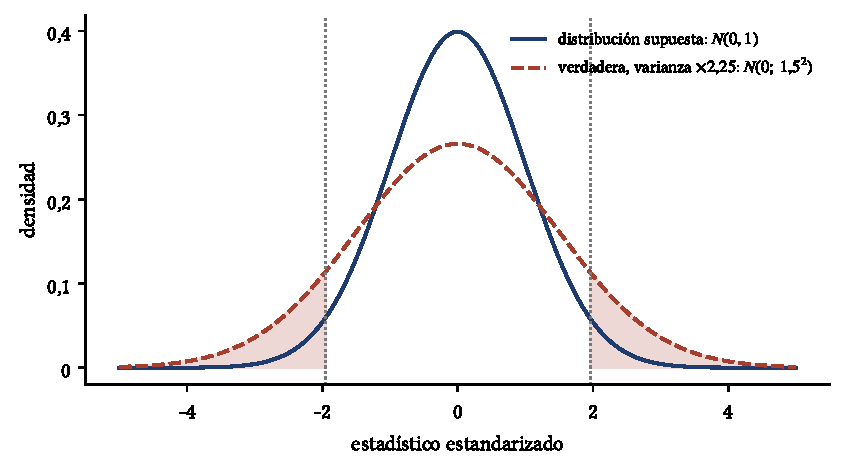
\includegraphics[width=0.78\linewidth]{graficos/cap16_fig_varianza_inducida.pdf}
\caption{Si el evento aumenta la varianza a $1{,}5^2$ pero la prueba supone $N(0,1)$, el área sombreada fuera de $\pm1{,}96$ es
la probabilidad real de rechazo bajo la hipótesis nula: 0,191 en lugar de 0,05.}
\label{fig:varinducida}
\end{figure}

\begin{observacion}
Las pruebas de este capítulo sirven para horizontes cortos. Para horizontes de meses o años, los errores del modelo de
rendimiento normal se acumulan, los rendimientos acumulados son muy asimétricos y la elección del modelo domina el
resultado (Barber y Lyon, 1997; Kothari y Warner, 2007).
\end{observacion}

% ---------------------------------------------------------------------
\section{Ejercicios resueltos}
% ---------------------------------------------------------------------

\begin{ejresuelto}{Los resultados de Facebook de julio de 2018}\label{ej:facebook}
\enunciado Facebook publicó sus resultados del segundo trimestre de 2018 después del cierre del 25 de julio. Estime los
rendimientos anormales con los tres modelos de rendimiento normal, contraste el del día 0 y calcule los CAR de
$(-1,+1)$, $(0,+5)$ y $(-5,+5)$. Verifique la Proposición~\ref{prop:ficticia}.

\solucion
\paso{Paso 1. El día 0 y el modelo de mercado.} El día 0 es el 26 de julio de 2018, y la ventana de estimación va del 28 de
julio de 2017 al 11 de julio de 2018. La acción cayó $18{,}96$\,\% y el mercado, $0{,}30$\,\%. Con $\hat\alpha=0{,}0212$ y
$\hat\beta=1{,}2789$:
\begin{align*}
  AR_0 &= -18{,}9609-0{,}0212-1{,}2789\times(-0{,}3032)\\
       &= -18{,}9609-0{,}0212+0{,}3878\\
       &= -18{,}5943\text{\,\%}.
\end{align*}

\paso{Paso 2. Su error estándar.} Con $s=1{,}3389$, $\hat\mu_m=0{,}0507$ y $S_{mm}=153{,}80$, por la
Proposición~\ref{prop:varar}:
\begin{align*}
  (R_{m0}-\hat\mu_m)^2 &= (-0{,}3032-0{,}0507)^2\\
                      &= 0{,}1253,\\
  1+\tfrac1{240}+\tfrac{0{,}1253}{153{,}80} &= 1+0{,}004167+0{,}000814\\
                                         &= 1{,}004981,\\
  \text{ee}(AR_0) &= 1{,}3389\sqrt{1{,}004981}\\
                  &= 1{,}3422,\\
  t &= \frac{-18{,}5943}{1{,}3422}\\
    &= -13{,}85 .
\end{align*}
El valor crítico de la $t_{238}$ al 5\,\% es 1,970: la caída es unas 14 desviaciones estándar de un día normal.

\paso{Paso 3. Comparación de modelos.}
\begin{center}\small
\begin{tabular}{@{}lrrrrrr@{}}
\toprule
Modelo & $s$ & $AR_0$ & $t$ & $CAR(-1,+1)$ & $CAR(0,+5)$ & $CAR(-5,+5)$ \\
\midrule
Mercado & 1,339 & $-18{,}59$ & $-13{,}85$ & $-18{,}42$ & $-18{,}11$ & $-15{,}76$ \\
Media constante & 1,685 & $-19{,}05$ & $-11{,}28$ & $-18{,}68$ & $-19{,}34$ & $-15{,}93$ \\
Ajustado por mercado & 1,352 & $-18{,}66$ & $-13{,}80$ & $-18{,}37$ & $-18{,}17$ & $-15{,}41$ \\
\bottomrule
\end{tabular}
\end{center}
Los tres modelos coinciden en la magnitud, porque el mercado casi no se movió ese día. La diferencia está en la
precisión: el modelo de mercado reduce la desviación estándar de 1,685 a 1,339 y aumenta el estadístico $t$. Ningún otro día
de la ventana es significativo; el mayor, $+2{,}10$\,\% el 2 de agosto, tiene $t=1{,}56$ (Figura~\ref{fig:facebook}).

\paso{Paso 4. La ficticia.} La regresión de la ventana de estimación más el día 0, con una ficticia del día 0, da $\hat\delta=-18{,}5943$
y ee $=1{,}3422$, idénticos a los pasos 1 y 2.

\paso{Paso 5. Una ventana de estimación contaminada.} La ventana incluye el caso Cambridge Analytica de marzo de 2018
(Ejercicio~\ref{ej:cambridge}). Excluyendo del 19 al 26 de marzo, $s$ baja a 1,2844 y $t$ sube a $-14{,}47$; la conclusión no cambia,
pero muestra que los días con eventos propios deben quitarse de la estimación.

\codigoweb{cap16_ej01}
\salidaR{cap16_ej01_R.txt}
\lectura{cap16_ej01}

\RvsPy La función \texttt{rendimientos\_normales} devuelve en ambos lenguajes el vector de $AR$ y la matriz $V$ completa del
Corolario~\ref{cor:varcar}, de modo que cualquier CAR se obtiene con $\boldsymbol\gamma'\mathbf{AR}$ y $\sqrt{\boldsymbol\gamma'V\boldsymbol\gamma}$. La
regresión con la ficticia se hace con \texttt{lm} en R y con álgebra matricial en Python. Los índices difieren en uno
(R empieza en 1), por eso el R imprime \texttt{t0 - 1} como posición.

\begin{figure}[ht]
\centering
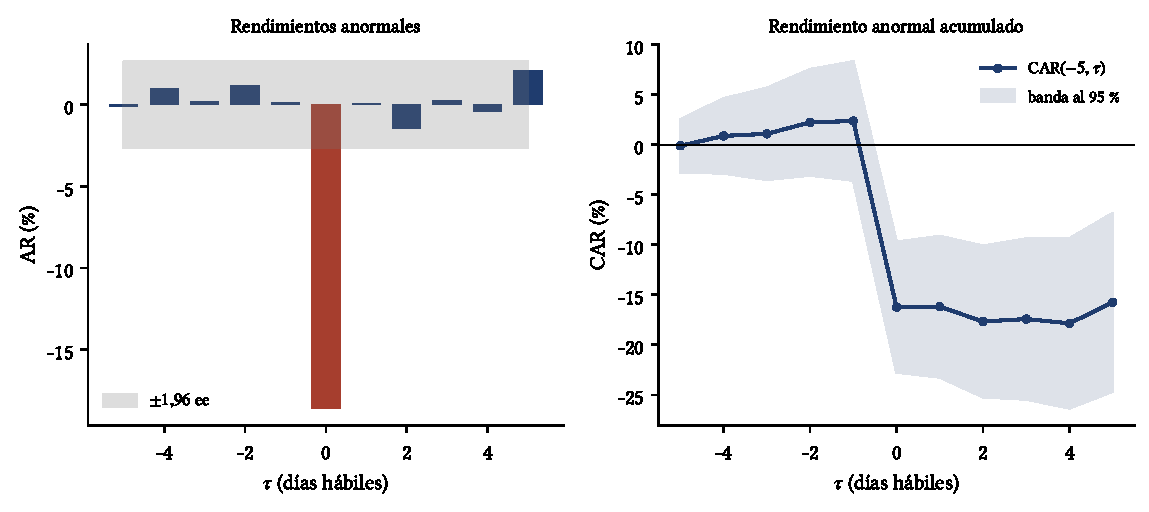
\includegraphics[width=\linewidth]{graficos/cap16_ej01_facebook.pdf}
\caption{Facebook alrededor del 26 de julio de 2018 (modelo de mercado). Izquierda: rendimientos anormales diarios con la
banda de $\pm1{,}96$ errores estándar. Derecha: CAR desde $\tau=-5$ con su banda al 95\,\%.}
\label{fig:facebook}
\end{figure}

\begin{conclusion}
El anuncio destruyó cerca del 18,6\,\% del valor de Facebook en un día, sin reversión en la semana siguiente. Cuando el
efecto es así de grande, el modelo de rendimiento normal casi no importa; importa cuando el efecto es pequeño, que es el caso
habitual.
\end{conclusion}
\end{ejresuelto}

\begin{ejresuelto}{Cambridge Analytica y el contagio}\label{ej:cambridge}
\enunciado El sábado 17 de marzo de 2018 se publicó que la consultora Cambridge Analytica había obtenido datos de millones de
usuarios de Facebook. Con el lunes 19 de marzo como día 0, mida el efecto en Facebook y en Apple, Amazon y Alphabet. ¿Hubo
contagio al resto del sector? Use la cartera de pares para la prueba conjunta.

\solucion
\paso{Paso 1. Efecto por empresa} (modelo de mercado).
\begin{center}\small
\begin{tabular}{@{}lrrrrrrr@{}}
\toprule
 & $\hat\beta$ & $AR_0$ & $t$ & $CAR(0,+1)$ & $t$ & $CAR(0,+5)$ & $t$ \\
\midrule
FB   & 1,235 & $-5{,}05$ & $-4{,}74$ & $-7{,}83$ & $-5{,}21$ & $-10{,}25$ & $-3{,}88$ \\
AAPL & 1,227 & 0,18 & 0,18 & $-0{,}08$ & $-0{,}06$ & 1,07 & 0,44 \\
AMZN & 1,071 & $-0{,}37$ & $-0{,}27$ & 1,98 & 1,05 & 1,67 & 0,50 \\
GOOG & 1,358 & $-1{,}27$ & $-1{,}46$ & $-1{,}69$ & $-1{,}39$ & $-2{,}98$ & $-1{,}39$ \\
\bottomrule
\end{tabular}
\end{center}
Facebook perdió un 10,2\,\% anormal en seis días; ninguno de los pares tiene un efecto significativo.

\paso{Paso 2. La prueba conjunta de los pares.} Los tres eventos tienen la misma fecha y sus residuos están
correlacionados (0,32, 0,30 y 0,47). La cartera igualmente ponderada da $CAR(0,+5)=-0{,}078$ con ee $=2{,}012$. La prueba ingenua,
que supone independencia, usa ee $=1{,}547$. El cociente es
\begin{align*}
  \frac{2{,}0118}{1{,}5467} &= 1{,}301,
\end{align*}
cercano al que predice la Proposición~\ref{prop:agrupado} con la correlación media $\bar\rho=0{,}361$ y $N=3$:
\begin{align*}
  \sqrt{1+(3-1)\times0{,}361} &= \sqrt{1{,}723}\\
                             &= 1{,}313 .
\end{align*}
Aquí no cambia la conclusión (no hay contagio), pero con muchas empresas y un efecto pequeño la prueba ingenua rechazaría
con demasiada frecuencia.

\paso{Paso 3. Facebook frente a sus pares.} El rendimiento de FB menos el de la cartera de pares, con el modelo de media, tiene
$CAR(0,+5)=-10{,}23$ y $t=-4{,}35$: el golpe fue propio de Facebook (Figura~\ref{fig:cambridge}).

\codigoweb{cap16_ej02}
\salidaR{cap16_ej02_R.txt}
\lectura{cap16_ej02}

\RvsPy La cartera se forma promediando los rendimientos fila por fila: \texttt{rowMeans} en R, \texttt{mean(1)} en Python. Los
residuos de la estimación quedan guardados en el componente \texttt{e} del resultado, lo que permite calcular su correlación
sin volver a estimar.

\begin{figure}[ht]
\centering
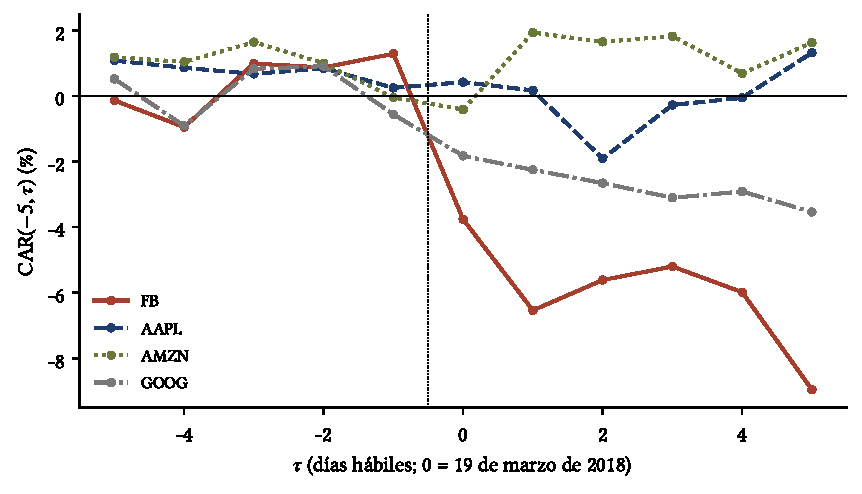
\includegraphics[width=0.8\linewidth]{graficos/cap16_ej02_cambridge.pdf}
\caption{CAR desde $\tau=-5$ de las cuatro empresas alrededor del 19 de marzo de 2018. Solo Facebook se separa de cero.}
\label{fig:cambridge}
\end{figure}

\begin{conclusion}
Cuando varios activos comparten la fecha del evento, la prueba correcta trata la cartera como una sola observación. El
escándalo afectó a Facebook y no al resto de las grandes tecnológicas.
\end{conclusion}
\end{ejresuelto}

\begin{ejresuelto}{Los anuncios del FOMC y el S\&P 500}\label{ej:fomc}
\enunciado Con las 40 reuniones programadas del FOMC de 2014 a 2018, estudie el S\&P 500 entre $\tau=-5$ y $+5$ del día del
comunicado. Use el modelo de media constante (el índice es el propio mercado), las cinco pruebas y la regresión con ficticias
de los días $-1$ y $0$ en toda la muestra.

\solucion
\paso{Paso 1. Rendimiento anormal medio por día.}
\begin{center}\small
\begin{tabular}{@{}rrrrrrr@{}}
\toprule
$\tau$ & $\overline{AR}$ & $J_1$ & Patell & BMP & Signo & $N^+/N$ \\
\midrule
$-2$ & $-0{,}218$ & $-1{,}75$ & $-1{,}83$ & $-2{,}17$ & $-2{,}53$ & 12/40 \\
$-1$ & 0,176 & 1,42 & 1,16 & 1,25 & 1,90 & 26/40 \\
0    & $-0{,}029$ & $-0{,}23$ & $-0{,}20$ & $-0{,}22$ & $-1{,}58$ & 15/40 \\
$+1$ & $-0{,}128$ & $-1{,}03$ & $-1{,}14$ & $-0{,}92$ & $-0{,}63$ & 18/40 \\
\bottomrule
\end{tabular}
\end{center}
El día del anuncio no hay efecto medio ($-0{,}03$\,\%; Corrado $=-0{,}92$). La víspera el índice subió $0{,}18$\,\% más que lo
normal, con 26 de 40 días positivos, pero no es significativo al 5\,\%. Los $CAAR$ de las ventanas $(-1,0)$, $(0,+5)$ y $(-5,+5)$
tampoco lo son ($J_1=0{,}84$, $-1{,}27$ y $-1{,}04$).

\paso{Paso 2. Interpretación de $\tau=-2$.} BMP y signo rechazan en $\tau=-2$. Pero se probaron 11 días: con 11 pruebas al 5\,\%,
la probabilidad de al menos un rechazo falso, si fueran independientes, es
\begin{align*}
  1-0{,}95^{11} &= 1-0{,}5688\\
               &= 0{,}431 .
\end{align*}
Un rechazo aislado en un día sin justificación económica previa no es evidencia convincente.

\paso{Paso 3. Regresión con ficticias.} En los 1\,258 días de 2014 a 2018, con errores de White:
\begin{align*}
  r_t = \underset{(0{,}0245)}{0{,}0216}+\underset{(0{,}1073)}{0{,}1986}\,D_t^{(-1)}-\underset{(0{,}1191)}{0{,}0067}\,D_t^{(0)} .
\end{align*}
La víspera del anuncio rinde 0,20 puntos más que un día normal ($t=1{,}85$). Lucca y Moench (2015) documentaron un
\emph{drift} previo al FOMC mucho mayor entre 1994 y 2011, concentrado en las 24 horas antes del comunicado; con cierres
diarios y estos cinco años el efecto es menor y no significativo al 5\,\%. Además, la desviación estándar del día del anuncio
(0,747) es \emph{menor} que la de los días normales (0,841): no hay varianza inducida (Figura~\ref{fig:fomc}).

\codigoweb{cap16_ej03}
\salidaR{cap16_ej03_R.txt}
\lectura{cap16_ej03}

\RvsPy Las fechas se localizan con \texttt{match} en R y con \texttt{np.where} en Python. Como el día 0 de cada evento tiene su
propia ventana de estimación, las 40 estimaciones se hacen con \texttt{lapply} o con una comprensión de listas, y los $AR$ se
apilan en una matriz $40\times11$. Los errores de White se calculan a mano, $(X'X)^{-1}X'\mathrm{diag}(e^2)X(X'X)^{-1}$.

\begin{figure}[ht]
\centering
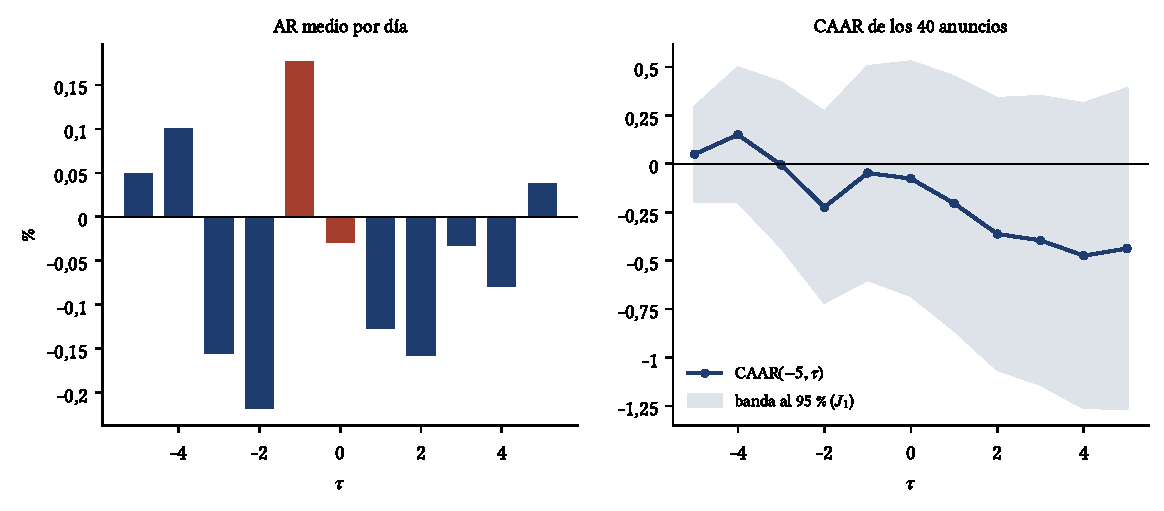
\includegraphics[width=\linewidth]{graficos/cap16_ej03_fomc.pdf}
\caption{S\&P 500 alrededor de los 40 comunicados del FOMC de 2014 a 2018. Izquierda: rendimiento anormal medio por día (en
rojo, la víspera y el día del anuncio). Derecha: CAAR con la banda al 95\,\% de $J_1$.}
\label{fig:fomc}
\end{figure}

\begin{conclusion}
Entre 2014 y 2018 los comunicados del FOMC no movieron el S\&P 500 en promedio. Un efecto nulo es un resultado tan válido
como uno significativo; lo importante es no buscar día por día hasta encontrar un rechazo.
\end{conclusion}
\end{ejresuelto}

\begin{ejresuelto}{Tamaño y potencia de las pruebas}\label{ej:potencia}
\enunciado Repita el diseño de Brown y Warner (1985) con datos reales: forme 1\,000 muestras de $N=20$ eventos, cada uno una
acción elegida al azar entre las cuatro y una fecha al azar entre 1\,007 posibles. Agregue un rendimiento anormal
$\delta\in\{0;\ 0{,}5;\ 1;\ 2\}$\,\% al día 0 y calcule la frecuencia de rechazo al 5\,\% de cada prueba.

\solucion
\paso{Paso 1. Resultados.}
\begin{center}\small
\begin{tabular}{@{}rrrrrr@{}}
\toprule
$\delta$ (\%) & $J_1$ & Patell & BMP & Signo & Corrado \\
\midrule
0,0 & 0,053 & 0,060 & 0,066 & 0,042 & 0,057 \\
0,5 & 0,362 & 0,440 & 0,526 & 0,467 & 0,638 \\
1,0 & 0,930 & 0,964 & 0,937 & 0,940 & 0,992 \\
2,0 & 1,000 & 1,000 & 0,992 & 1,000 & 1,000 \\
\bottomrule
\end{tabular}
\end{center}

\paso{Paso 2. Tamaño.} Con $\delta=0$, todas rechazan cerca del 5\,\%. Con 1\,000 muestras, el error estándar de una frecuencia de
0,05 es
\begin{align*}
  \sqrt{\frac{0{,}05\times0{,}95}{1\,000}} &= \sqrt{0{,}0000475}\\
                                         &= 0{,}0069,
\end{align*}
así que el 6,6\,\% de BMP está algo por encima. Se debe a usar 1,96 en lugar del valor crítico de la $t_{19}$, que es 2,09; con
$N=20$ la diferencia importa.

\paso{Paso 3. Potencia.} Con $\delta=0{,}5$\,\%, la prueba de rangos de Corrado detecta el efecto en el 64\,\% de las muestras y
$J_1$ solo en el 36\,\%. La razón está en la distribución de los rendimientos anormales: su asimetría es 1,14 y sus colas son
pesadas. Las pruebas paramétricas pierden potencia con valores extremos, que inflan la varianza estimada; los rangos no se
ven afectados. Patell y BMP superan a $J_1$ porque ponderan más los activos menos volátiles (Figura~\ref{fig:potencia}).

\codigoweb{cap16_ej04}
\salidaR{cap16_ej04_R.txt}
\lectura{cap16_ej04}

\RvsPy Los generadores aleatorios de R y de NumPy son distintos, así que las mismas instrucciones darían muestras distintas.
Para reproducir los resultados exactamente en ambos lenguajes usamos un generador propio, el congruencial de Park y Miller
(1988), $x\leftarrow16\,807\,x \bmod (2^{31}-1)$. Los productos no pasan de $3{,}6\times10^{13}$, menos que $2^{53}$, de modo que la
aritmética de doble precisión de R es exacta. Ese generador sirve para enseñar, no para simulaciones serias, que deben usar
los generadores modernos de cada lenguaje. Los rendimientos anormales de las 4\,028 combinaciones posibles se calculan una
sola vez antes de la simulación.

\begin{figure}[ht]
\centering
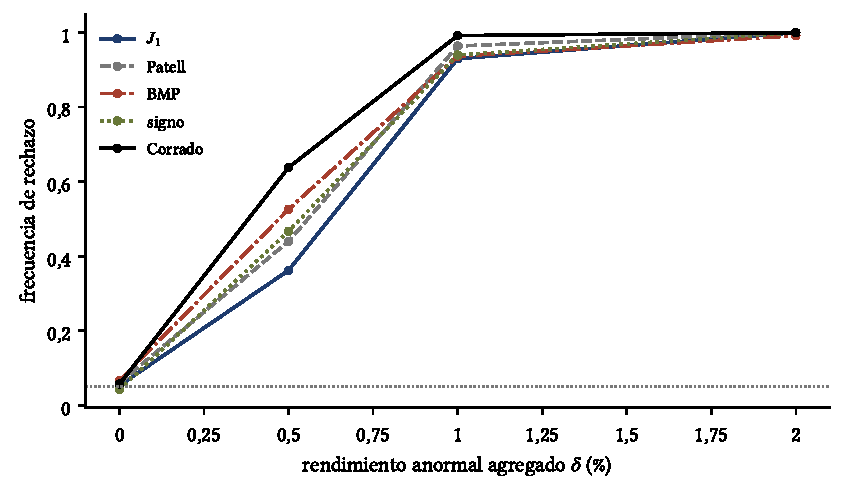
\includegraphics[width=0.78\linewidth]{graficos/cap16_ej04_potencia.pdf}
\caption{Frecuencia de rechazo al 5\,\% de cada prueba según el rendimiento anormal agregado, con 1\,000 muestras de 20 eventos.
La línea punteada marca el 5\,\% nominal.}
\label{fig:potencia}
\end{figure}

\begin{conclusion}
Con rendimientos diarios de acciones individuales, todas las pruebas tienen el tamaño correcto, pero la de rangos es
claramente más potente para efectos pequeños. Conviene informar al menos una prueba paramétrica y una no paramétrica.
\end{conclusion}
\end{ejresuelto}

\begin{ejresuelto}{Varianza inducida por el evento}\label{ej:varinducida}
\enunciado (a) Repita la simulación del Ejercicio~\ref{ej:potencia}, pero ahora el evento multiplica por 2,25 la varianza del
día 0: a cada $AR$ se le suma un ruido normal de varianza $1{,}25\,\hat\sigma_i^2$. (b) Estudie el cambio porcentual del VIX
alrededor de los anuncios del FOMC.

\solucion
\paso{Paso 1. La simulación.}
\begin{center}\small
\begin{tabular}{@{}rrrrrr@{}}
\toprule
$\delta$ (\%) & $J_1$ & Patell & BMP & Signo & Corrado \\
\midrule
0,0 & 0,216 & 0,217 & 0,078 & 0,057 & 0,143 \\
1,0 & 0,823 & 0,861 & 0,681 & 0,475 & 0,782 \\
\bottomrule
\end{tabular}
\end{center}
Sin efecto en la media, $J_1$ y Patell rechazan el 22\,\% de las veces, muy cerca del 19,1\,\% que predice la
Proposición~\ref{prop:varinducida}. BMP se mantiene cerca del 5\,\% (el exceso, como antes, se debe al valor crítico) y la prueba
del signo también. La de rangos, que era la mejor sin varianza inducida, rechaza el 14\,\%: los valores extremos del día 0
obtienen rangos extremos con más frecuencia de la que supone su denominador. Con $\delta=1$\,\%, la potencia de BMP (0,68) es
menor que la de $J_1$, pero esta última se logra a costa de rechazar demasiado bajo la nula.

\paso{Paso 2. El VIX y el FOMC.}
\begin{center}\small
\begin{tabular}{@{}rrrrrr@{}}
\toprule
$\tau$ & $\overline{AR}$ (\%) & $J_1$ & BMP & $N^+/N$ & $\widehat{\Var}(SAR)$ \\
\midrule
$-2$ & 3,54 & 2,80 & 2,67 & 25/40 & 0,969 \\
$-1$ & $-1{,}68$ & $-1{,}33$ & $-1{,}34$ & 18/40 & 0,840 \\
0    & $-1{,}48$ & $-1{,}17$ & $-1{,}27$ & 19/40 & 0,970 \\
$+3$ & 1,66 & 1,31 & 0,80 & 21/40 & 4,066 \\
\bottomrule
\end{tabular}
\end{center}
El VIX tiende a bajar la víspera y el día del anuncio: $CAAR(-1,0)=-3{,}16$\,\%, con $J_1=-1{,}76$ y BMP $=-2{,}02$, en el límite de la
significancia. La varianza de corte transversal de los $SAR$ en el día 0 es 0,97, cercana a uno: los anuncios no aumentaron la
dispersión. En $\tau=+3$ es 4,07 por un solo evento: el 5 de febrero de 2018, tres días hábiles después del comunicado del 31
de enero, el VIX subió 76,8\,\% en logaritmos, en el desplome de los productos de volatilidad inversa. Ahí $J_1$ (1,31) y BMP (0,80)
difieren justamente porque BMP usa esa dispersión en el denominador. El rechazo en $\tau=-2$ tiene el mismo problema de
pruebas múltiples que en el Ejercicio~\ref{ej:fomc} (Figura~\ref{fig:vix}).

\codigoweb{cap16_ej05}
\salidaR{cap16_ej05_R.txt}
\lectura{cap16_ej05}

\RvsPy Los ruidos normales se generan con el método de Box y Muller:
\[
  z=\sqrt{-2\ln u_1}\,\cos(2\pi u_2),
\]
a partir de dos uniformes del generador de Park y Miller; así R y Python reciben los mismos
números. En R, la matriz \texttt{s[, 1:2]} de pares (acción, fecha) sirve directamente como índice de la matriz \texttt{AR0}.

\begin{figure}[ht]
\centering
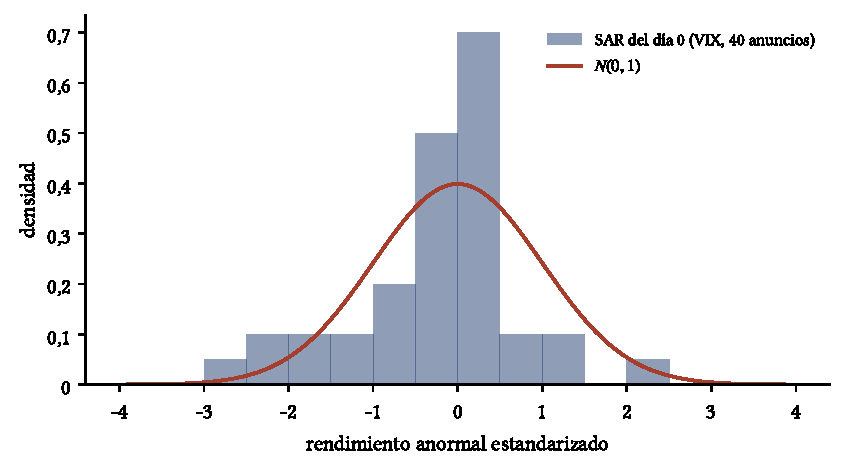
\includegraphics[width=0.78\linewidth]{graficos/cap16_ej05_vix.pdf}
\caption{Histograma de los rendimientos anormales estandarizados del VIX en el día de los 40 anuncios del FOMC, con la
densidad $N(0,1)$ que suponen las pruebas.}
\label{fig:vix}
\end{figure}

\begin{conclusion}
Cuando un evento puede aumentar la volatilidad, que es lo habitual en anuncios de resultados o fusiones, las pruebas que usan
la varianza de la ventana de estimación rechazan demasiado. BMP es la opción paramétrica segura, y la de rangos debe
interpretarse con cuidado.
\end{conclusion}
\end{ejresuelto}

% ---------------------------------------------------------------------
\section{Ejercicios propuestos}
% ---------------------------------------------------------------------

\begin{enumerate}[label=\textbf{\thechapter.\arabic*},leftmargin=*,itemsep=6pt]
  \item Con $L_1=240$, $s=1{,}2$, $R_{m0}=2$, $\hat\mu_m=0{,}05$ y $S_{mm}=240$, calcule el error estándar de $AR_0$ en el modelo de
  mercado. \textit{Respuesta: el factor es $1{,}02001$; ee $=1{,}2119$.}

  \item Con $N=30$ eventos, $L_1-2=238$ y $\sum_iSAR_i=12$, calcule el estadístico de Patell. \textit{Respuesta: $12/\sqrt{30{,}254}=2{,}182$.}

  \item Diez empresas con el mismo día de evento tienen rendimientos anormales con correlación $0{,}3$. ¿Por qué factor subestima
  la prueba ingenua el error estándar del promedio? \textit{Respuesta: $\sqrt{1+9\times0{,}3}=1{,}924$.}

  \item Demuestre que en el modelo ajustado por mercado, con $\sigma^2$ estimada con la varianza de $R_i-R_m$ en la ventana de estimación,
  $\Var(CAR(\tau_1,\tau_2))=(\tau_2-\tau_1+1)\sigma^2$, y explique por qué no hay término de error de estimación.

  \item Demuestre que, bajo la hipótesis nula y con $AR_i$ independientes y de mediana cero, el estadístico del signo converge a
  $N(0,1)$.

  \item \emph{(Simulación.)} Repita el Ejercicio~\ref{ej:potencia} con $N=50$. ¿Se reduce el exceso de rechazo de BMP? ¿Cambia el orden de
  potencia de las pruebas?

  \item \emph{(Con datos de la BVL.)} Elija un anuncio relevante de una empresa peruana (por ejemplo, un cambio de calificación
  crediticia o un anuncio de dividendos) y estudie su efecto con el índice S\&P/BVL Perú General como mercado. Discuta el
  problema de la negociación poco frecuente: ¿qué pasa con $\hat\beta$ si la acción no cotiza todos los días? (Scholes y Williams, 1977.)

  \item \emph{(Con datos.)} Repita el Ejercicio~\ref{ej:facebook} con una ventana de estimación de 120 días, $\tau=-130,\dots,-11$. ¿Cambian
  $\hat\beta$, $s$ y el estadístico $t$?
\end{enumerate}

% ---------------------------------------------------------------------
\section{Resumen de fórmulas}
% ---------------------------------------------------------------------

\begin{table}[H]
\centering\small
\begin{tabular}{@{}ll@{}}
\toprule
Concepto & Fórmula \\
\midrule
Rendimiento anormal & $AR_{i\tau}=R_{i\tau}-\hat\alpha_i-\hat\beta_iR_{m\tau}$;\quad $CAR_i(\tau_1,\tau_2)=\sum_{\tau=\tau_1}^{\tau_2}AR_{i\tau}$ \\
Varianza del AR & $\sigma^2\bigl[1+\frac1{L_1}+\frac{(R_{m\tau}-\hat\mu_m)^2}{S_{mm}}\bigr]$ \\
Varianza del vector AR & $V_i=\sigma^2[I+X^*(X'X)^{-1}X^{*\prime}]$;\quad $\Var(CAR)=\boldsymbol\gamma'V_i\boldsymbol\gamma$ \\
Ficticia & $R_{it}=\alpha_i+\beta_iR_{mt}+\delta D_t+u_t$;\quad $\hat\delta=AR_{i\tau}$ \\
$J_1$ & $\overline{AR}/\sqrt{\sum_i\hat\sigma_i^2/N^2}$ \\
Patell & $\sum_iSAR_i/\sqrt{\sum_ig/(g-2)}$ \\
BMP & $\overline{SAR}/(s_{SAR}/\sqrt N)$ \\
Signo & $(N^+-N/2)/\sqrt{N/4}$ \\
Eventos simultáneos & $\Var(\overline{AR})=\frac{\sigma^2}{N}[1+(N-1)\rho]$ \\
Varianza inducida & $J_1$, Patell $\to N(0,c)$;\quad BMP $\to N(0,1)$ \\
\bottomrule
\end{tabular}
\caption{Fórmulas principales del Capítulo 16.}
\end{table}

\section*{Referencias}
\begin{itemize}[leftmargin=*]
  \item Barber, B. M. y Lyon, J. D. (1997). Detecting long-run abnormal stock returns: The empirical power and specification
        of test statistics. \emph{Journal of Financial Economics}, 43(3), 341--372.
  \item Boehmer, E., Musumeci, J. y Poulsen, A. B. (1991). Event-study methodology under conditions of event-induced
        variance. \emph{Journal of Financial Economics}, 30(2), 253--272.
  \item Brown, S. J. y Warner, J. B. (1985). Using daily stock returns: The case of event studies. \emph{Journal of Financial
        Economics}, 14(1), 3--31.
  \item Campbell, J. Y., Lo, A. W. y MacKinlay, A. C. (1997). \emph{The Econometrics of Financial Markets}, cap. 4. Princeton
        University Press.
  \item Corrado, C. J. (1989). A nonparametric test for abnormal security-price performance in event studies. \emph{Journal
        of Financial Economics}, 23(2), 385--395.
  \item Fama, E. F., Fisher, L., Jensen, M. C. y Roll, R. (1969). The adjustment of stock prices to new information.
        \emph{International Economic Review}, 10(1), 1--21.
  \item Kothari, S. P. y Warner, J. B. (2007). Econometrics of event studies. En B. E. Eckbo (ed.), \emph{Handbook of
        Corporate Finance}, vol. 1, 3--36. Elsevier.
  \item Lucca, D. O. y Moench, E. (2015). The pre-FOMC announcement drift. \emph{Journal of Finance}, 70(1), 329--371.
  \item MacKinlay, A. C. (1997). Event studies in economics and finance. \emph{Journal of Economic Literature}, 35(1), 13--39.
  \item Park, S. K. y Miller, K. W. (1988). Random number generators: Good ones are hard to find. \emph{Communications of the
        ACM}, 31(10), 1192--1201.
  \item Patell, J. M. (1976). Corporate forecasts of earnings per share and stock price behavior: Empirical tests.
        \emph{Journal of Accounting Research}, 14(2), 246--276.
  \item Scholes, M. y Williams, J. (1977). Estimating betas from nonsynchronous data. \emph{Journal of Financial Economics},
        5(3), 309--327.
\end{itemize}

% =====================================================================
%  Capítulo 17. Modelos con cambios de régimen de Markov
% =====================================================================
\chapter[Cambios de régimen de Markov]{Modelos con cambios de régimen de Markov}\label{cap:markov}

\section*{Objetivos de aprendizaje}
Al terminar este capítulo, el lector podrá:
\begin{enumerate}[label=\arabic*.,leftmargin=*]
  \item Describir una cadena de Markov de dos estados: probabilidades estacionarias, duraciones esperadas y
        persistencia, y demostrar por qué una mezcla con regímenes persistentes produce colas pesadas y
        agrupamiento de volatilidad.
  \item Derivar el filtro de Hamilton, la verosimilitud que produce y el suavizador de Kim.
  \item Estimar los modelos con el algoritmo EM y obtener errores estándar con el hessiano numérico.
  \item Elegir el número de regímenes, interpretarlos frente a cronologías externas como la del NBER y usar el
        modelo para pronosticar y medir el riesgo.
\end{enumerate}

\section*{Motivación}
Los mercados alternan períodos largos de calma con episodios breves de pánico: 1929--1933, 1974, 1987, 2008. Los
modelos GARCH del Capítulo~\ref{cap:garch} describen esa alternancia con una varianza que cambia de forma continua.
Hamilton (1989) propuso otra idea: la economía está en uno de unos pocos \emph{regímenes} (expansión y recesión,
calma y crisis), cada uno con sus propios parámetros, y salta de uno a otro según una cadena de Markov que no se
observa. El econometrista nunca sabe con certeza en qué régimen está, pero puede calcular su probabilidad con los
datos. Ese cálculo, el filtro de Hamilton, es una aplicación directa del teorema de Bayes y la base de este capítulo.

\paragraph{Datos del capítulo.} El exceso de rendimiento mensual del mercado de acciones de EE.\,UU. (factor Mkt-RF de
Kenneth French), de julio de 1926 a noviembre de 2018 ($T=1\,109$); la variación porcentual trimestral del índice de
producción industrial de EE.\,UU. (FRED), de 1970T1 a 2019T2 ($T=198$); y la cronología de picos y valles del ciclo
económico del NBER.

% ---------------------------------------------------------------------
\section{La cadena de Markov}
% ---------------------------------------------------------------------

Sea $s_t\in\{1,\dots,K\}$ el régimen en el período $t$. La cadena es de Markov si el régimen de mañana depende solo
del de hoy:
\[
  \Pr(s_t=j\mid s_{t-1}=i,s_{t-2},\dots)=\Pr(s_t=j\mid s_{t-1}=i)=p_{ij}.
\]
Las probabilidades de transición forman la matriz $P=[p_{ij}]$, cuyas filas suman uno. Con dos regímenes,
\[
  P=\begin{bmatrix}p_{11} & 1-p_{11}\\ 1-p_{22} & p_{22}\end{bmatrix}.
\]

\begin{proposicion}[Propiedades de la cadena de dos estados]\label{prop:cadena}
Si $0<p_{11},p_{22}<1$:
\begin{enumerate}[label=(\alph*)]
  \item La probabilidad estacionaria del régimen 1 es $\pi_1=\dfrac{1-p_{22}}{2-p_{11}-p_{22}}$.
  \item La duración de una estancia en el régimen $i$ es geométrica, con media $\E[D_i]=\dfrac{1}{1-p_{ii}}$.
  \item El indicador $\xi_t=\mathbb 1\{s_t=1\}$ sigue un AR(1): $\E[\xi_{t+1}\mid s_t]=(1-p_{22})+\lambda\,\xi_t$, con
        $\lambda=p_{11}+p_{22}-1$, y su autocorrelación de orden $k$ es $\lambda^k$.
\end{enumerate}
\end{proposicion}

\begin{proof}
(a) La distribución estacionaria cumple $\pi_1=\pi_1p_{11}+\pi_2(1-p_{22})$ y $\pi_2=1-\pi_1$:
\begin{align*}
  \pi_1 &= \pi_1p_{11}+(1-\pi_1)(1-p_{22})\\
  \pi_1 &= \pi_1p_{11}+1-p_{22}-\pi_1+\pi_1p_{22}\\
  \pi_1(2-p_{11}-p_{22}) &= 1-p_{22}\\
  \pi_1 &= \frac{1-p_{22}}{2-p_{11}-p_{22}}.
\end{align*}

(b) Una estancia dura exactamente $d$ períodos si la cadena permanece $d-1$ veces y luego sale:
$\Pr(D_i=d)=p_{ii}^{d-1}(1-p_{ii})$. Usando $\sum_{d\ge1}d\,x^{d-1}=1/(1-x)^2$:
\begin{align*}
  \E[D_i] &= \sum_{d=1}^{\infty}d\,p_{ii}^{d-1}(1-p_{ii})\\
          &= (1-p_{ii})\,\frac{1}{(1-p_{ii})^2}\\
          &= \frac{1}{1-p_{ii}}.
\end{align*}

(c) Si $s_t=1$, $\E[\xi_{t+1}]=p_{11}$; si $s_t=2$, $\E[\xi_{t+1}]=1-p_{22}$. Ambos casos en una fórmula:
\begin{align*}
  \E[\xi_{t+1}\mid s_t] &= p_{11}\,\xi_t+(1-p_{22})(1-\xi_t)\\
                        &= (1-p_{22})+(p_{11}+p_{22}-1)\,\xi_t\\
                        &= (1-p_{22})+\lambda\,\xi_t .
\end{align*}
Es la esperanza condicional de un AR(1) con coeficiente $\lambda$; iterando $k$ veces,
$\E[\xi_{t+k}-\pi_1\mid s_t]=\lambda^k(\xi_t-\pi_1)$, de donde $\operatorname{Corr}(\xi_{t+k},\xi_t)=\lambda^k$.
\end{proof}

Con $p_{11}=0{,}98$ y $p_{22}=0{,}90$, el régimen 1 dura en promedio 50 meses, el 2 dura 10 y la cadena pasa el 83\,\%
del tiempo en el régimen 1. Con $\lambda=0{,}88$ los regímenes son muy persistentes.

% ---------------------------------------------------------------------
\section{El modelo de mezcla con regímenes de Markov}
% ---------------------------------------------------------------------

El modelo más simple con cambio de régimen es
\[
  y_t=\mu_{s_t}+\sigma_{s_t}\varepsilon_t,\qquad \varepsilon_t\sim\text{i.i.d. }N(0,1),
\]
con $\varepsilon_t$ independiente de la cadena. Condicionada en el régimen, $y_t$ es normal; sin conocerlo, es una
\emph{mezcla} de normales con pesos $\pi_j$.

\begin{proposicion}[Momentos de la mezcla]\label{prop:mezcla}
En el estado estacionario, con $\bar\mu=\sum_j\pi_j\mu_j$:
\begin{enumerate}[label=(\alph*)]
  \item $\E[y_t]=\bar\mu$ y $\Var(y_t)=\sum_j\pi_j\sigma_j^2+\sum_j\pi_j(\mu_j-\bar\mu)^2$.
  \item Si $\mu_1=\mu_2$ y $\sigma_1\neq\sigma_2$, la curtosis es mayor que 3.
  \item Si $\mu_1=\mu_2=0$, $\Cov(y_t^2,y_{t-k}^2)=(\sigma_1^2-\sigma_2^2)^2\,\pi_1\pi_2\,\lambda^k$.
\end{enumerate}
\end{proposicion}

\begin{proof}
(a) Por la ley de la varianza total, condicionando en el régimen:
\begin{align*}
  \Var(y_t) &= \E\bigl[\Var(y_t\mid s_t)\bigr]+\Var\bigl(\E[y_t\mid s_t]\bigr)\\
            &= \sum_j\pi_j\sigma_j^2+\sum_j\pi_j(\mu_j-\bar\mu)^2 .
\end{align*}

(b) Con media común $\mu$, sean $m_2=\sum_j\pi_j\sigma_j^2$ y $m_4=\E[(y_t-\mu)^4]$. Como el cuarto momento de una normal es
$3\sigma^4$:
\begin{align*}
  m_4 &= \sum_j\pi_j\,3\sigma_j^4\\
      &= 3\,\E[\sigma_{s_t}^4]\\
      &> 3\,\bigl(\E[\sigma_{s_t}^2]\bigr)^2\\
      &= 3\,m_2^2,
\end{align*}
donde la desigualdad es la de Jensen ($\Var(\sigma^2_{s_t})>0$ porque las varianzas difieren). La curtosis es
$m_4/m_2^2>3$.

(c) Con $\mu_j=0$, $\E[y_t^2\mid s_t]=\sigma_{s_t}^2=\sigma_2^2+(\sigma_1^2-\sigma_2^2)\,\xi_t$. Como los $\varepsilon$ son independientes
de la cadena y entre sí, para $k\ge1$:
\begin{align*}
  \Cov(y_t^2,y_{t-k}^2) &= \Cov\bigl(\E[y_t^2\mid s],\ \E[y_{t-k}^2\mid s]\bigr)\\
                        &= \Cov\bigl(\sigma_2^2+(\sigma_1^2-\sigma_2^2)\xi_t,\ \sigma_2^2+(\sigma_1^2-\sigma_2^2)\xi_{t-k}\bigr)\\
                        &= (\sigma_1^2-\sigma_2^2)^2\,\Cov(\xi_t,\xi_{t-k})\\
                        &= (\sigma_1^2-\sigma_2^2)^2\,\pi_1\pi_2\,\lambda^k,
\end{align*}
usando $\Var(\xi_t)=\pi_1\pi_2$ y la parte (c) de la Proposición~\ref{prop:cadena}.
\end{proof}

La proposición explica por qué estos modelos encajan con los hechos estilizados del Capítulo~\ref{cap:hechos}: la mezcla
genera colas pesadas, y la persistencia de los regímenes genera autocorrelación positiva y lenta de los cuadrados, es
decir, agrupamiento de volatilidad. La Figura~\ref{fig:regimenes} lo muestra con $\mu=(1;\,-0{,}5)$, $\sigma=(3{,}5;\,8)$,
$p_{11}=0{,}98$ y $p_{22}=0{,}90$: la mezcla tiene curtosis 5,63, frente a 3 de la normal con la misma media y varianza.

\begin{figure}[ht]
\centering
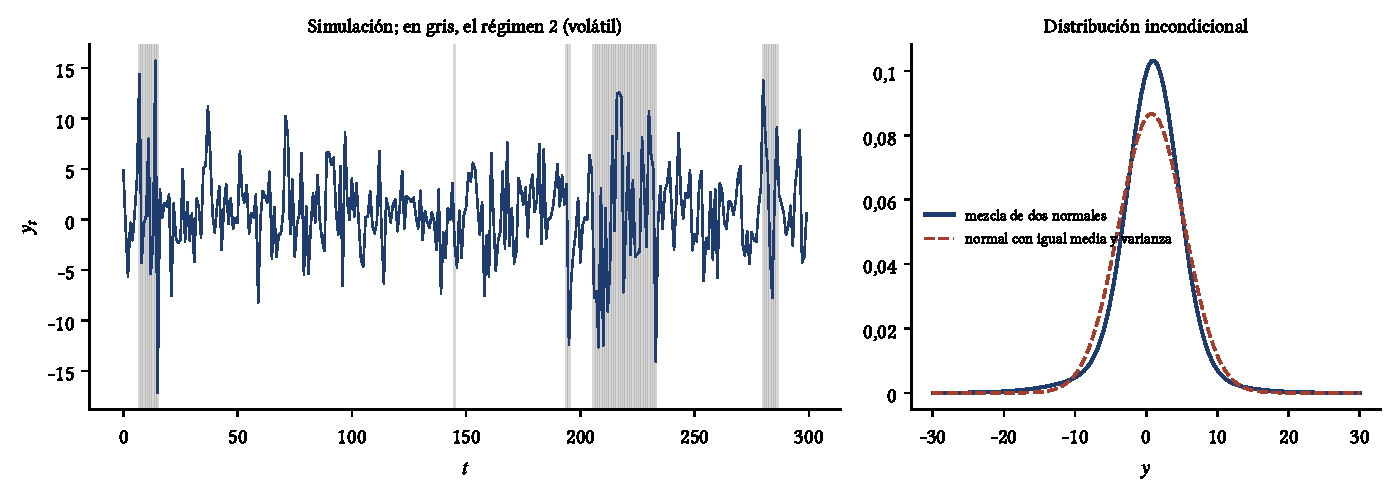
\includegraphics[width=\linewidth]{graficos/cap17_fig_regimenes.pdf}
\caption{Izquierda: 300 observaciones simuladas de un modelo con dos regímenes; en gris, los períodos en el régimen
volátil. Derecha: la distribución incondicional (mezcla) frente a la normal de igual media y varianza: más alta en el
centro y con colas más gruesas.}
\label{fig:regimenes}
\end{figure}

% ---------------------------------------------------------------------
\section{El filtro de Hamilton}
% ---------------------------------------------------------------------

Sean $\mathcal Y_t=(y_1,\dots,y_t)$ la información hasta $t$, $\eta_{jt}=f(y_t\mid s_t=j,\mathcal Y_{t-1})$ la densidad en el
régimen $j$ (en el modelo de mezcla, $\phi\bigl((y_t-\mu_j)/\sigma_j\bigr)/\sigma_j$) y los vectores de probabilidades
\[
  \boldsymbol\xi_{t\mid t-1}=\bigl[\Pr(s_t=j\mid\mathcal Y_{t-1})\bigr]_j\ \ \text{(predichas)},\qquad
  \boldsymbol\xi_{t\mid t}=\bigl[\Pr(s_t=j\mid\mathcal Y_t)\bigr]_j\ \ \text{(filtradas)}.
\]

\begin{proposicion}[Filtro de Hamilton]\label{prop:hamilton}
Partiendo de $\boldsymbol\xi_{1\mid0}=\boldsymbol\rho$, para $t=1,\dots,T$:
\[
  f(y_t\mid\mathcal Y_{t-1})=\sum_j\xi_{j,t\mid t-1}\,\eta_{jt},\qquad
  \xi_{j,t\mid t}=\frac{\xi_{j,t\mid t-1}\,\eta_{jt}}{f(y_t\mid\mathcal Y_{t-1})},\qquad
  \boldsymbol\xi_{t+1\mid t}=P'\boldsymbol\xi_{t\mid t},
\]
y la log-verosimilitud es $\ell=\sum_{t=1}^T\ln f(y_t\mid\mathcal Y_{t-1})$.
\end{proposicion}

\begin{proof}
La densidad de $y_t$ dada la historia se obtiene sumando sobre el régimen (ley de probabilidad total):
\begin{align*}
  f(y_t\mid\mathcal Y_{t-1}) &= \sum_j f(y_t,s_t=j\mid\mathcal Y_{t-1})\\
                             &= \sum_j\Pr(s_t=j\mid\mathcal Y_{t-1})\,f(y_t\mid s_t=j,\mathcal Y_{t-1})\\
                             &= \sum_j\xi_{j,t\mid t-1}\,\eta_{jt}.
\end{align*}
La actualización es el teorema de Bayes:
\begin{align*}
  \Pr(s_t=j\mid\mathcal Y_t) &= \frac{f(y_t,s_t=j\mid\mathcal Y_{t-1})}{f(y_t\mid\mathcal Y_{t-1})}\\
                             &= \frac{\xi_{j,t\mid t-1}\,\eta_{jt}}{f(y_t\mid\mathcal Y_{t-1})}.
\end{align*}
La predicción usa la propiedad de Markov, $\Pr(s_{t+1}=j\mid s_t=i,\mathcal Y_t)=p_{ij}$:
\begin{align*}
  \Pr(s_{t+1}=j\mid\mathcal Y_t) &= \sum_i\Pr(s_t=i\mid\mathcal Y_t)\,p_{ij}\\
                                 &= \bigl[P'\boldsymbol\xi_{t\mid t}\bigr]_j .
\end{align*}
Finalmente, la densidad conjunta se factoriza en condicionales:
\begin{align*}
  \ln f(y_1,\dots,y_T) &= \ln\prod_{t=1}^Tf(y_t\mid\mathcal Y_{t-1})\\
                       &= \sum_{t=1}^T\ln f(y_t\mid\mathcal Y_{t-1}).
\end{align*}
\end{proof}

\begin{proposicion}[Suavizador de Kim]\label{prop:kim}
Con $\boldsymbol\xi_{T\mid T}$ del filtro, hacia atrás para $t=T-1,\dots,1$:
\[
  \xi_{i,t\mid T}=\xi_{i,t\mid t}\sum_j p_{ij}\,\frac{\xi_{j,t+1\mid T}}{\xi_{j,t+1\mid t}},\qquad
  \Pr(s_t=i,s_{t+1}=j\mid\mathcal Y_T)=\frac{\xi_{i,t\mid t}\,p_{ij}\,\xi_{j,t+1\mid T}}{\xi_{j,t+1\mid t}}.
\]
\end{proposicion}

\begin{proof}
El paso clave es que, conocido $s_{t+1}$, las observaciones futuras no informan sobre $s_t$:
$\Pr(s_t=i\mid s_{t+1}=j,\mathcal Y_T)=\Pr(s_t=i\mid s_{t+1}=j,\mathcal Y_t)$, porque $y_{t+1},\dots,y_T$ dependen de $s_t$ solo
a través de $s_{t+1}$ (supuesto exacto en el modelo de mezcla y en el MSI-AR del Ejercicio~\ref{ej:produccion}). Por Bayes:
\begin{align*}
  \Pr(s_t=i\mid s_{t+1}=j,\mathcal Y_t) &= \frac{\Pr(s_t=i\mid\mathcal Y_t)\,\Pr(s_{t+1}=j\mid s_t=i)}{\Pr(s_{t+1}=j\mid\mathcal Y_t)}\\
                                         &= \frac{\xi_{i,t\mid t}\,p_{ij}}{\xi_{j,t+1\mid t}}.
\end{align*}
Multiplicando por $\Pr(s_{t+1}=j\mid\mathcal Y_T)$ se obtiene la probabilidad conjunta, y sumando sobre $j$, la marginal:
\begin{align*}
  \Pr(s_t=i,s_{t+1}=j\mid\mathcal Y_T) &= \frac{\xi_{i,t\mid t}\,p_{ij}\,\xi_{j,t+1\mid T}}{\xi_{j,t+1\mid t}},\\
  \xi_{i,t\mid T} &= \sum_j\frac{\xi_{i,t\mid t}\,p_{ij}\,\xi_{j,t+1\mid T}}{\xi_{j,t+1\mid t}}\\
                  &= \xi_{i,t\mid t}\sum_jp_{ij}\,\frac{\xi_{j,t+1\mid T}}{\xi_{j,t+1\mid t}}.
\end{align*}
\end{proof}

Las probabilidades \emph{filtradas} usan solo el pasado y son las que habría calculado un inversionista en tiempo
real; las \emph{suavizadas} usan toda la muestra y son las adecuadas para fechar los regímenes después.

% ---------------------------------------------------------------------
\section{Estimación por el algoritmo EM}
% ---------------------------------------------------------------------

La verosimilitud de la Proposición~\ref{prop:hamilton} puede maximizarse numéricamente, pero tiene muchos óptimos
locales y restricciones ($0<p_{ij}<1$, $\sigma_j>0$). El algoritmo EM (Dempster, Laird y Rubin, 1977; Hamilton, 1990)
es más estable: si los regímenes se observaran, estimar el modelo sería trivial; como no se observan, se sustituyen
por sus probabilidades suavizadas y se itera.

\begin{proposicion}[Paso M del modelo de mezcla]\label{prop:em}
Dadas las probabilidades suavizadas $\hat\xi_{jt}=\Pr(s_t=j\mid\mathcal Y_T)$ y
$\hat n_{ij}=\sum_{t=2}^T\Pr(s_{t-1}=i,s_t=j\mid\mathcal Y_T)$ calculadas con los parámetros actuales, los valores que
maximizan la log-verosimilitud completa esperada son
\[
  \hat\mu_j=\frac{\sum_t\hat\xi_{jt}\,y_t}{\sum_t\hat\xi_{jt}},\qquad
  \hat\sigma_j^2=\frac{\sum_t\hat\xi_{jt}\,(y_t-\hat\mu_j)^2}{\sum_t\hat\xi_{jt}},\qquad
  \hat p_{ij}=\frac{\hat n_{ij}}{\sum_k\hat n_{ik}} .
\]
\end{proposicion}

\begin{proof}
Si los regímenes se observaran, la log-verosimilitud completa sería
$\sum_t\sum_j\mathbb 1\{s_t=j\}\ln\eta_{jt}+\sum_t\sum_{i,j}\mathbb 1\{s_{t-1}=i,s_t=j\}\ln p_{ij}$, más un término de la
probabilidad inicial. Su esperanza condicional en los datos sustituye los indicadores por las probabilidades suavizadas:
\[
  Q=\sum_t\sum_j\hat\xi_{jt}\Bigl[-\tfrac12\ln(2\pi\sigma_j^2)-\frac{(y_t-\mu_j)^2}{2\sigma_j^2}\Bigr]+\sum_{i,j}\hat n_{ij}\ln p_{ij}.
\]
Para $\mu_j$:
\begin{align*}
  \frac{\partial Q}{\partial\mu_j} &= \sum_t\hat\xi_{jt}\,\frac{y_t-\mu_j}{\sigma_j^2}=0\\
  \sum_t\hat\xi_{jt}\,y_t &= \mu_j\sum_t\hat\xi_{jt}\\
  \hat\mu_j &= \frac{\sum_t\hat\xi_{jt}\,y_t}{\sum_t\hat\xi_{jt}}.
\end{align*}
Para $\sigma_j^2$:
\begin{align*}
  \frac{\partial Q}{\partial\sigma_j^2} &= \sum_t\hat\xi_{jt}\Bigl[-\frac{1}{2\sigma_j^2}+\frac{(y_t-\mu_j)^2}{2\sigma_j^4}\Bigr]=0\\
  \sigma_j^2\sum_t\hat\xi_{jt} &= \sum_t\hat\xi_{jt}(y_t-\mu_j)^2 .
\end{align*}
Para cada fila $i$ de $P$ maximizamos $\sum_j\hat n_{ij}\ln p_{ij}$ sujeto a $\sum_jp_{ij}=1$, con el lagrangiano
$\sum_j\hat n_{ij}\ln p_{ij}-\kappa(\sum_jp_{ij}-1)$:
\begin{align*}
  \frac{\hat n_{ij}}{p_{ij}}-\kappa &= 0\\
  p_{ij} &= \hat n_{ij}/\kappa\\
  \sum_jp_{ij}=1 &\ \Rightarrow\ \kappa=\sum_k\hat n_{ik}\\
  \hat p_{ij} &= \frac{\hat n_{ij}}{\sum_k\hat n_{ik}} .
\end{align*}
\end{proof}

El paso M es una media y una varianza \emph{ponderadas} por la probabilidad de cada régimen, y la transición estimada es
la frecuencia esperada de pasar de $i$ a $j$. Cada iteración EM no disminuye la verosimilitud; se itera hasta que el
aumento sea menor que $10^{-10}$. En el modelo MSI-AR del Ejercicio~\ref{ej:produccion}, con intercepto cambiante y
$\phi$ y $\sigma$ comunes, el paso M es una regresión de mínimos cuadrados ponderados con una ficticia por régimen.

\begin{observacion}[Identificación y número de regímenes]
Los regímenes solo están definidos salvo una permutación: cambiar los nombres de 1 y 2 da la misma verosimilitud. Se
fija el orden con una regla, por ejemplo $\sigma_1<\sigma_2$. Contrastar $K=1$ frente a $K=2$ con la razón de
verosimilitudes no es estándar: bajo la hipótesis nula, $p_{11}$ y $p_{22}$ no están identificados y el estadístico no
sigue una $\chi^2$ (Hansen, 1992; Garcia, 1998). En la práctica se usan criterios de información, el bootstrap
paramétrico o, como en el Ejercicio~\ref{ej:numero}, contrastes \emph{dentro} de un modelo con el mismo número de regímenes,
que sí son estándar.
\end{observacion}

% ---------------------------------------------------------------------
\section{Ejercicios resueltos}
% ---------------------------------------------------------------------

\begin{ejresuelto}{Dos regímenes en el mercado de EE.\,UU.}\label{ej:mercado2}
\enunciado Estime por EM el modelo $y_t=\mu_{s_t}+\sigma_{s_t}\varepsilon_t$ con dos regímenes para el exceso de rendimiento
mensual del mercado de 1926 a 2018. Calcule errores estándar con el hessiano numérico, las probabilidades estacionarias, las
duraciones y los momentos implícitos, y compare con la normal.

\solucion
\paso{Paso 1. Estimaciones.} El EM converge en 53 iteraciones a $\ell=-3\,256{,}22$:
\begin{center}\small
\begin{tabular}{@{}lrrlrr@{}}
\toprule
 & Régimen 1 (tranquilo) & ee & & Régimen 2 (volátil) & ee \\
\midrule
$\mu_j$ (\%) & 1,009 & 0,143 & & $-1{,}430$ & 0,880 \\
$\sigma_j$ (\%) & 3,741 & 0,133 & & 10,456 & 0,864 \\
$p_{jj}$ & 0,9842 & 0,007 & & 0,9058 & 0,037 \\
\bottomrule
\end{tabular}
\end{center}
En el régimen tranquilo el mercado rinde un 1,01\,\% mensual sobre la tasa libre de riesgo con una volatilidad de 3,7\,\%;
en el volátil, la volatilidad casi se triplica y el rendimiento medio es negativo, aunque impreciso.

\paso{Paso 2. Persistencia.} Por la Proposición~\ref{prop:cadena}:
\begin{align*}
  \E[D_1] &= \frac{1}{1-0{,}9842}\\
          &= 63{,}3\ \text{meses},\\
  \E[D_2] &= \frac{1}{1-0{,}9058}\\
          &= 10{,}6\ \text{meses},\\
  \pi_1 &= \frac{1-0{,}9058}{2-0{,}9842-0{,}9058}\\
        &= \frac{0{,}0942}{0{,}1100}\\
        &= 0{,}856 .
\end{align*}
El mercado pasa el 86\,\% del tiempo en calma, en episodios de más de cinco años, y el 14\,\% en crisis que duran en promedio
casi un año ($\lambda=0{,}89$).

\paso{Paso 3. Momentos y ajuste.} El modelo reproduce la media (0,659) y la desviación estándar (5,329) de la muestra, e
implica una curtosis de 7,52 frente a 10,90 en los datos: captura gran parte de las colas pesadas, aunque no todas. La
log-verosimilitud mejora en 172,1 puntos sobre la normal (Figura~\ref{fig:densidad17}). La razón de Sharpe mensual es 0,27
en el régimen tranquilo y $-0{,}14$ en el volátil (Figura~\ref{fig:prob17}).

\codigoweb{cap17_ej01}
\salidaR{cap17_ej01_R.txt}
\lectura{cap17_ej01}

\RvsPy El filtro, el suavizador y el EM están programados igual en ambos lenguajes y producen las mismas cifras. El EM es
determinista: con los mismos valores iniciales y el mismo criterio de parada, R y Python recorren las mismas iteraciones. Los
errores estándar salen de un hessiano numérico por diferencias centrales y difieren en la cuarta decimal por redondeo; por eso
se imprimen con tres. Como verificación, \texttt{statsmodels} (\texttt{MarkovRegression} con \texttt{switching\_variance=True}),
que maximiza la verosimilitud directamente y fija la probabilidad inicial en la estacionaria, da $\ell=-3\,256{,}37$,
$\mu=(1{,}007;\,-1{,}435)$ y $\sigma=(3{,}743;\,10{,}470)$ (archivo \texttt{cap17\_ej01\_statsmodels.py}). La pequeña diferencia en $\ell$ se
debe a que nuestro EM estima también la probabilidad inicial.

\begin{figure}[ht]
\centering
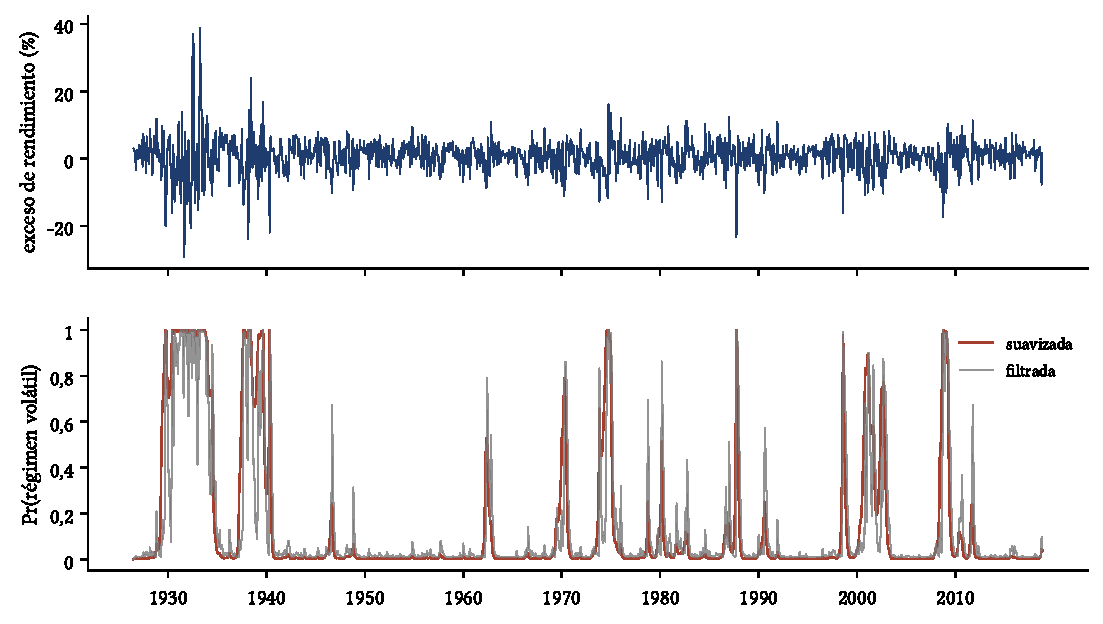
\includegraphics[width=\linewidth]{graficos/cap17_ej01_probabilidades.pdf}
\caption{Arriba: exceso de rendimiento mensual del mercado. Abajo: probabilidad del régimen volátil, filtrada (gris) y
suavizada (rojo). Destacan los episodios de 1929--1934, 1937--1940, 1974, 2000--2002 y 2008--2009.}
\label{fig:prob17}
\end{figure}

\begin{figure}[ht]
\centering
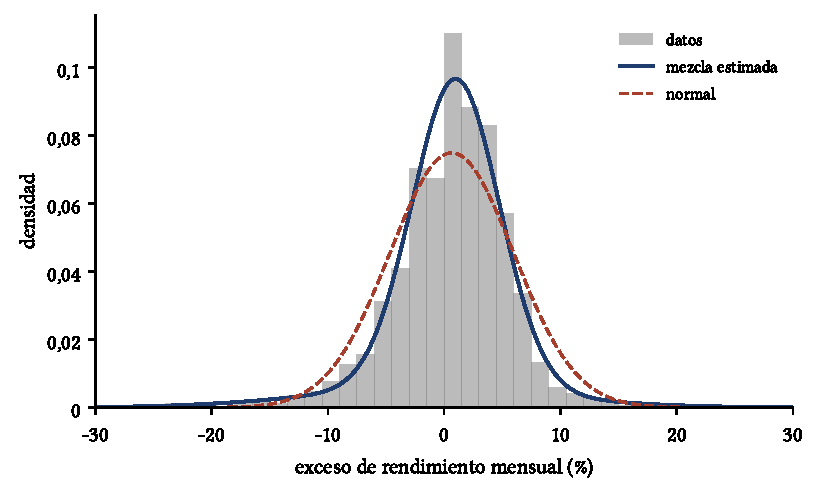
\includegraphics[width=0.75\linewidth]{graficos/cap17_ej01_densidad.pdf}
\caption{Histograma de los rendimientos con la mezcla estimada y la normal de igual media y varianza.}
\label{fig:densidad17}
\end{figure}

\begin{conclusion}
Dos regímenes bastan para describir la mayor parte de las colas pesadas y del agrupamiento de volatilidad del mercado
estadounidense: un régimen largo y tranquilo con prima positiva y otro corto y turbulento con prima negativa.
\end{conclusion}
\end{ejresuelto}

\begin{ejresuelto}{El régimen volátil y las recesiones}\label{ej:nber}
\enunciado Compare la probabilidad suavizada del régimen volátil del Ejercicio~\ref{ej:mercado2} con la cronología de recesiones del
NBER (un mes está en recesión desde el mes siguiente al pico hasta el valle). Identifique los episodios volátiles de seis meses
o más.

\solucion
\paso{Paso 1. Asociación.} Hay 199 meses de recesión en la muestra. La probabilidad media del régimen volátil es 0,437 en
recesión y 0,079 en expansión, y la correlación con el indicador de recesión es 0,466.
\begin{center}\small
\begin{tabular}{@{}lrr@{}}
\toprule
NBER & Tranquilo & Volátil \\
\midrule
Expansión & 852 & 58 \\
Recesión & 110 & 89 \\
\bottomrule
\end{tabular}
\end{center}
\begin{align*}
  \Pr(\text{volátil}\mid\text{recesión}) &= \frac{89}{199}\\
                                       &= 0{,}447,\\
  \Pr(\text{volátil}\mid\text{expansión}) &= \frac{58}{910}\\
                                        &= 0{,}064 .
\end{align*}

\paso{Paso 2. Episodios.}
\begin{center}\small
\begin{tabular}{@{}llrrrr@{}}
\toprule
Inicio & Fin & Meses & Media (\%) & Desv.\ est.\ (\%) & Meses en recesión \\
\midrule
1929-05 & 1934-07 & 63 & $-0{,}71$ & 12,77 & 43 \\
1937-06 & 1939-10 & 29 & 0,13 & 9,69 & 13 \\
1970-01 & 1970-06 & 6 & $-4{,}62$ & 5,28 & 6 \\
1974-03 & 1975-01 & 11 & $-2{,}09$ & 8,46 & 11 \\
2000-09 & 2001-09 & 13 & $-3{,}31$ & 5,36 & 6 \\
2008-08 & 2009-04 & 9 & $-3{,}35$ & 8,82 & 9 \\
\bottomrule
\end{tabular}
\end{center}
La Gran Depresión, la recesión de 1937--1938, la crisis petrolera de 1974, el fin de la burbuja tecnológica y la crisis
financiera de 2008 son regímenes volátiles. Pero muchas recesiones de posguerra (1948, 1953, 1957, 1960, 1981--1982, 1990)
tienen probabilidad casi nula: no todas las recesiones son crisis bursátiles, y no todas las crisis bursátiles son recesiones
(Figura~\ref{fig:nber}).

\codigoweb{cap17_ej02}
\salidaR{cap17_ej02_R.txt}
\lectura{cap17_ej02}

\RvsPy Los episodios consecutivos se encuentran en R con \texttt{rle} (\emph{run-length encoding}), que devuelve la longitud
y el valor de cada racha; en Python, con un bucle que avanza mientras el régimen no cambia. Las fechas en formato
\texttt{AAAA-MM} se comparan como texto: el orden alfabético coincide con el cronológico.

\begin{figure}[ht]
\centering
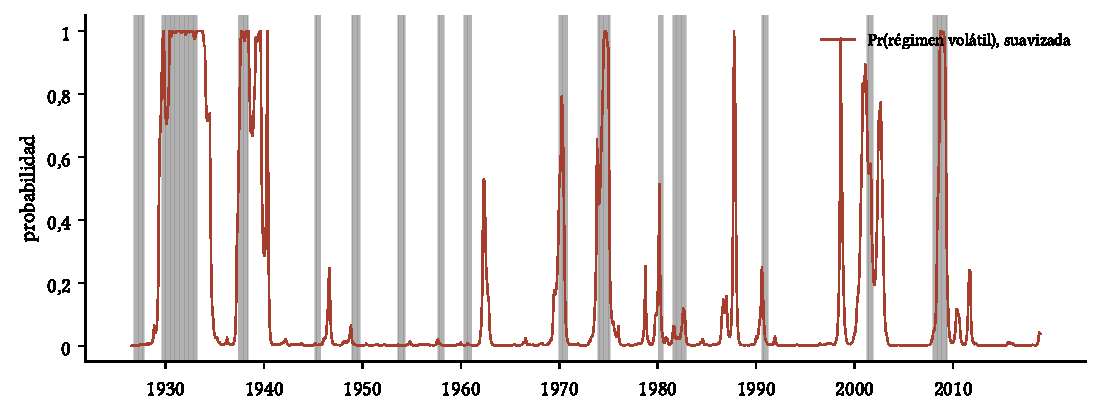
\includegraphics[width=\linewidth]{graficos/cap17_ej02_nber.pdf}
\caption{Probabilidad suavizada del régimen volátil y recesiones del NBER (franjas grises).}
\label{fig:nber}
\end{figure}

\begin{conclusion}
El régimen volátil está asociado con las recesiones, pero no las identifica: lo determinan las crisis financieras más que el
ciclo real. Fechar el ciclo exige un modelo para una variable real, que es el ejercicio siguiente.
\end{conclusion}
\end{ejresuelto}

\begin{ejresuelto}{El ciclo de la producción industrial}\label{ej:produccion}
\enunciado Con la variación trimestral de la producción industrial de 1970 a 2019, estime (A) el modelo MSI-AR(1)
$y_t=c_{s_t}+\phi\,y_{t-1}+\sigma\varepsilon_t$, con varianza común, y (B) el modelo de media y varianza cambiantes. Compare
ambos con los 29 trimestres de recesión del NBER (un trimestre está en recesión si al menos dos de sus meses lo están).

\solucion
\paso{Paso 1. Modelo A.} El AR(1) lineal tiene $\hat\phi=0{,}579$ y $\ell=-319{,}23$. El MSI-AR(1) mejora la verosimilitud a
$\ell=-299{,}37$ con $c_1=-3{,}671$, $c_2=0{,}440$, $\phi=0{,}431$ y $\sigma=0{,}998$. Pero su régimen 1 dura en promedio
\begin{align*}
  \frac{1}{1-0{,}4722} &= 1{,}89\ \text{trimestres}
\end{align*}
y solo clasifica 6 trimestres: los desplomes de 1974--1975, 1980, 1981 y 2008--2009. El modelo usa el segundo régimen para
acomodar los valores extremos, no para describir el ciclo.

\paso{Paso 2. Modelo B.} Con media y varianza cambiantes, $\ell=-319{,}45$:
\begin{center}\small
\begin{tabular}{@{}lrrrr@{}}
\toprule
Régimen & $\mu_j$ & $\sigma_j$ & $p_{jj}$ & Duración (trim.) \\
\midrule
1 (recesión) & $-1{,}452$ & 1,901 & 0,7749 & 4,44 \\
2 (expansión) & 0,984 & 0,907 & 0,9503 & 20,13 \\
\bottomrule
\end{tabular}
\end{center}
Ahora el régimen 1 es una recesión típica: la producción cae 1,45\,\% por trimestre durante algo más de un año. De los 36 trimestres
clasificados en recesión, 25 coinciden con el NBER, hay 11 falsas alarmas (seis de ellas en la contracción industrial de 2015--2016,
que el NBER no consideró recesión) y solo 4 recesiones no detectadas. La concordancia es 0,924 y la correlación con el indicador
NBER, 0,802 (Figura~\ref{fig:produccion}).

\paso{Paso 3. ¿Cuál es mejor?} A tiene mayor verosimilitud, pero B describe el ciclo. Las verosimilitudes no son del todo
comparables (A condiciona en la primera observación), y B ignora la autocorrelación dentro de cada régimen: la
autocorrelación de $y_t$ menos su media suavizada es aún 0,378. El modelo de Hamilton (1989), con intercepto y media cambiantes
en un AR(4), resuelve ambos problemas a costa de un paso M más complejo. La lección general es que la verosimilitud por sí sola
no garantiza que los regímenes tengan la interpretación buscada.

\codigoweb{cap17_ej03}
\salidaR{cap17_ej03_R.txt}
\lectura{cap17_ej03}

\RvsPy El paso M del MSI-AR resuelve un sistema de $K+1$ ecuaciones normales ponderadas, con \texttt{solve} en R y
\texttt{np.linalg.solve} en Python. Probamos 18 combinaciones de valores iniciales con el modelo A y 3 con el B, y en cada modelo todas
convergen al mismo máximo, lo que hace improbable que A sea un óptimo local. El indicador trimestral de recesión se construye a partir del mensual, con
\texttt{sprintf("\%s-\%02d", ...)} en R y una comprensión de listas en Python.

\begin{figure}[ht]
\centering
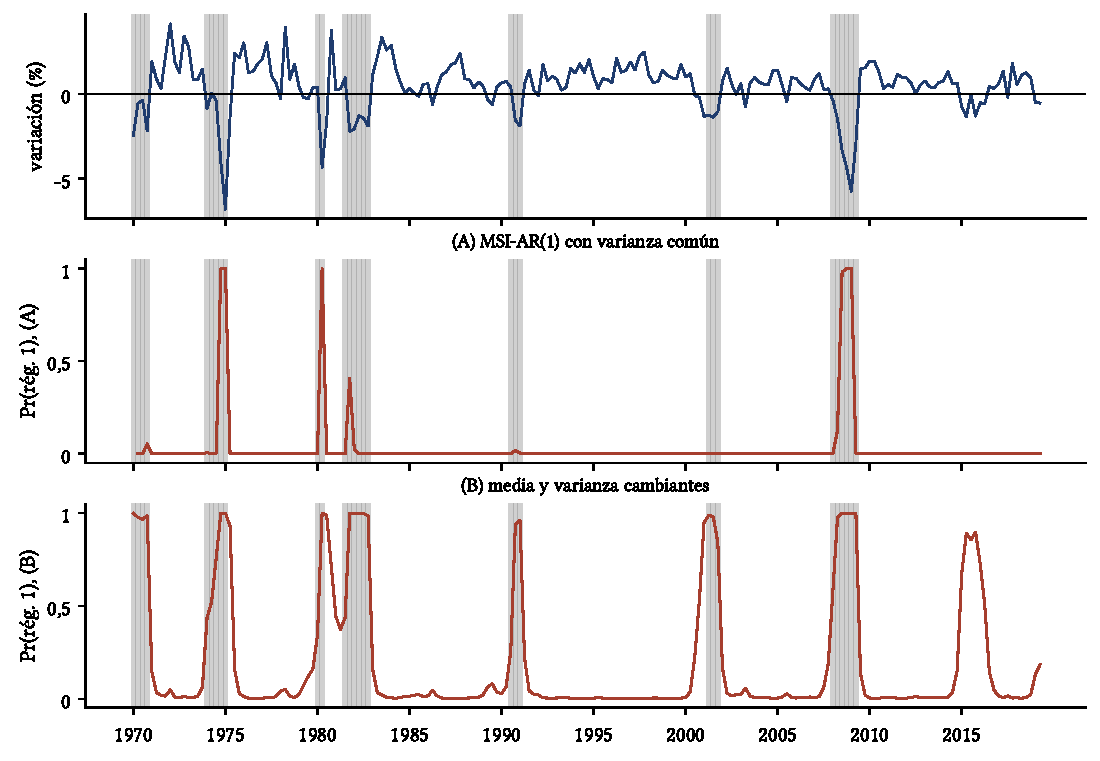
\includegraphics[width=\linewidth]{graficos/cap17_ej03_produccion.pdf}
\caption{Arriba: variación trimestral de la producción industrial. Al medio y abajo: probabilidad suavizada del régimen 1 en
los modelos A y B. Franjas grises: trimestres de recesión del NBER.}
\label{fig:produccion}
\end{figure}

\begin{conclusion}
Con media y varianza cambiantes, un modelo de dos regímenes reproduce la cronología del NBER sin usarla, a partir de una sola
serie. El modelo de mayor verosimilitud, en cambio, dedica un régimen a los valores atípicos.
\end{conclusion}
\end{ejresuelto}

\begin{ejresuelto}{¿Cuántos regímenes?}\label{ej:numero}
\enunciado Para el mercado, compare un régimen (normal), dos regímenes solo en la varianza, dos en media y varianza y tres en
media y varianza, con AIC y BIC. Contraste si las medias de los dos regímenes son iguales.

\solucion
\paso{Paso 1. Criterios de información.}
\begin{center}\small
\begin{tabular}{@{}lrrrr@{}}
\toprule
Modelo & $k$ & $\ell$ & AIC & BIC \\
\midrule
1 régimen (normal) & 2 & $-3\,428{,}33$ & 6\,860,67 & 6\,870,69 \\
2 regímenes, solo varianza & 5 & $-3\,260{,}73$ & 6\,531,45 & 6\,556,51 \\
2 regímenes, media y varianza & 6 & $-3\,256{,}22$ & 6\,524,45 & 6\,554,52 \\
3 regímenes, media y varianza & 12 & $-3\,234{,}26$ & 6\,492,52 & 6\,552,66 \\
\bottomrule
\end{tabular}
\end{center}
El salto de uno a dos regímenes es enorme; el de dos a tres es menor y el BIC apenas lo prefiere (por 1,86 puntos).

\paso{Paso 2. Medias iguales.} Con dos regímenes identificados por la varianza, la hipótesis $\mu_1=\mu_2$ es un contraste
estándar:
\begin{align*}
  LR &= 2\,\bigl[-3\,256{,}2248-(-3\,260{,}7262)\bigr]\\
     &= 2\times4{,}5014\\
     &= 9{,}003,
\end{align*}
con valor $p=0{,}0027$ en una $\chi^2_1$: el rendimiento medio sí cambia con el régimen.

\paso{Paso 3. Tres regímenes.} Aparecen un régimen muy tranquilo ($\sigma=2{,}72$, $\mu=1{,}22$), uno intermedio
($\sigma=4{,}52$, $\mu=0{,}67$) y uno de crisis ($\sigma=11{,}92$, $\mu=-1{,}29$), con duraciones de 24, 28 y 12 meses. La matriz de
transición es casi tridiagonal: de la calma no se salta directamente a la crisis (probabilidad estimada 0,0000), sino que se
pasa por el régimen intermedio (Figura~\ref{fig:tres}).

\codigoweb{cap17_ej04}
\salidaR{cap17_ej04_R.txt}
\lectura{cap17_ej04}

\RvsPy La función \texttt{em\_media\_varianza} sirve para cualquier $K$ y para el caso de media común
(\texttt{media\_comun}). En la tabla de salida el nombre del modelo va al final de cada línea: \texttt{sprintf} de R rellena
el ancho contando bytes, de modo que un nombre con tildes queda desalineado respecto de Python, que cuenta caracteres.

\begin{figure}[ht]
\centering
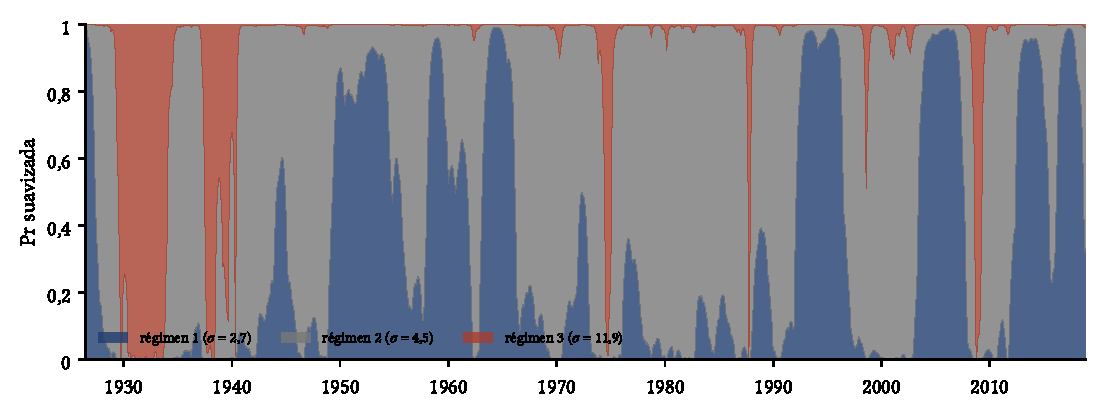
\includegraphics[width=\linewidth]{graficos/cap17_ej04_tres_regimenes.pdf}
\caption{Probabilidades suavizadas del modelo de tres regímenes, apiladas. El régimen de crisis (rojo) se concentra en
1929--1934, 1937--1940, 1974, 1987 y 2008--2009.}
\label{fig:tres}
\end{figure}

\begin{conclusion}
Los datos piden al menos dos regímenes que difieran en media y varianza. Un tercero mejora el ajuste y tiene una lectura
económica razonable, pero la evidencia a su favor es débil y, con 12 parámetros, sus estimaciones son menos estables.
\end{conclusion}
\end{ejresuelto}

\begin{ejresuelto}{Pronóstico y VaR con regímenes}\label{ej:var17}
\enunciado Con el modelo de dos regímenes, pronostique la media, la volatilidad y el VaR del mes siguiente a noviembre de 2018.
Luego evalúe el VaR mensual al 95 y al 99\,\% de 1926 a 2018 con las pruebas de Kupiec y de Christoffersen
(Capítulo~\ref{cap:var_riesgo}), frente al VaR de una normal con media y varianza constantes.

\solucion
\paso{Paso 1. Pronóstico.} La probabilidad filtrada del régimen volátil en noviembre de 2018 es 0,038, y la predicha para el mes
siguiente, $0{,}038\times0{,}9058+0{,}962\times0{,}0158=0{,}050$. La distribución predictiva es la mezcla con pesos
$(0{,}950;\,0{,}050)$:
\begin{align*}
  \E[y_{T+1}\mid\mathcal Y_T] &= 0{,}950\times1{,}009+0{,}050\times(-1{,}430)\\
                              &= 0{,}959-0{,}071\\
                              &= 0{,}887\,\text{\%},
\end{align*}
con desviación estándar 4,363\,\%. El VaR al 99\,\% de la mezcla, el cuantil que resuelve
$\sum_j w_j\Phi\bigl((q-\mu_j)/\sigma_j\bigr)=0{,}01$, es 10,80\,\%; el de la normal incondicional, 11,73\,\%.

\paso{Paso 2. Prueba retrospectiva.} En 1\,108 meses:
\begin{center}\small
\begin{tabular}{@{}llrrrrrr@{}}
\toprule
Nivel & Modelo & Excepciones & Esperadas & $LR_{uc}$ & $p$ & $LR_{ind}$ & $p$ \\
\midrule
5\,\% & Dos regímenes & 69 & 55,4 & 3,27 & 0,071 & 1,66 & 0,198 \\
5\,\% & Normal & 52 & 55,4 & 0,22 & 0,636 & 27,32 & 0,000 \\
1\,\% & Dos regímenes & 11 & 11,1 & 0,00 & 0,981 & 0,22 & 0,638 \\
1\,\% & Normal & 22 & 11,1 & 8,45 & 0,004 & 3,19 & 0,074 \\
\bottomrule
\end{tabular}
\end{center}
La normal acierta el número de excepciones al 5\,\%, pero las concentra en las crisis: la prueba de independencia la rechaza
con $LR_{ind}=27{,}3$. Al 1\,\% duplica las excepciones esperadas. El modelo de regímenes pasa ambas pruebas en los dos niveles,
porque su VaR al 99\,\% sube de 9\,\% en calma a más de 25\,\% en crisis (Figura~\ref{fig:var17}).

\paso{Paso 3. Una advertencia.} Los parámetros se estimaron con toda la muestra, de modo que la prueba retrospectiva usa
información que en 1930 no existía. Las probabilidades filtradas sí usan solo el pasado, pero una evaluación honesta debe
reestimar el modelo con datos disponibles en cada fecha (Ejercicio propuesto 17.8).

\codigoweb{cap17_ej05}
\salidaR{cap17_ej05_R.txt}
\lectura{cap17_ej05}

\RvsPy El cuantil de la mezcla se calcula por bisección con 200 pasos en $[-100;\,100]$, un método lento pero exacto y
determinista; \texttt{uniroot} en R y \texttt{scipy.optimize.brentq} en Python darían lo mismo con menos evaluaciones. La
función \texttt{kupiec\_christoffersen} trata el caso $0\ln0=0$, que ocurre cuando no hay dos excepciones seguidas.

\begin{figure}[ht]
\centering
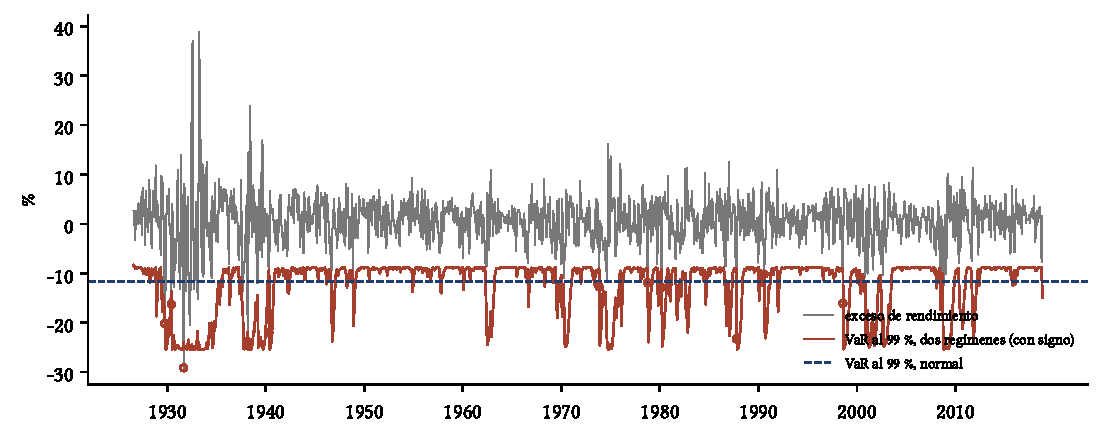
\includegraphics[width=\linewidth]{graficos/cap17_ej05_var.pdf}
\caption{Exceso de rendimiento mensual con el VaR al 99\,\% del modelo de dos regímenes (rojo, con sus excepciones marcadas) y
el de la normal (azul discontinua).}
\label{fig:var17}
\end{figure}

\begin{conclusion}
Un modelo de regímenes produce un VaR que se adapta a las crisis y supera las pruebas de cobertura e independencia donde el
modelo constante falla. Es una alternativa al GARCH con una interpretación directa: la probabilidad de estar en crisis.
\end{conclusion}
\end{ejresuelto}

% ---------------------------------------------------------------------
\section{Ejercicios propuestos}
% ---------------------------------------------------------------------

\begin{enumerate}[label=\textbf{\thechapter.\arabic*},leftmargin=*,itemsep=6pt]
  \item Con $p_{11}=0{,}95$ y $p_{22}=0{,}80$, calcule $\pi_1$, las duraciones esperadas y $\lambda$. \textit{Respuesta: $\pi_1=0{,}8$;
  20 y 5 períodos; $\lambda=0{,}75$.}

  \item Con $\boldsymbol\pi=(0{,}8;\,0{,}2)$, $\boldsymbol\mu=(1;\,-2)$ y $\boldsymbol\sigma=(4;\,10)$, calcule la media y la desviación estándar de
  la mezcla. \textit{Respuesta: $0{,}4$ y $\sqrt{34{,}24}=5{,}852$.}

  \item Con los parámetros del ejercicio anterior, $p_{11}=0{,}95$, $p_{22}=0{,}80$, $\boldsymbol\xi_{t-1\mid t-1}=(0{,}9;\,0{,}1)$ e
  $y_t=-8$, aplique un paso del filtro de Hamilton. \textit{Respuesta: $\boldsymbol\xi_{t\mid t-1}=(0{,}875;\,0{,}125)$;
  $\eta=(0{,}00793;\,0{,}03332)$; $\boldsymbol\xi_{t\mid t}=(0{,}625;\,0{,}375)$.}

  \item Demuestre que, si $\mu_1\neq\mu_2$ pero $\sigma_1=\sigma_2$, la mezcla también tiene autocorrelación en niveles:
  $\Cov(y_t,y_{t-k})=(\mu_1-\mu_2)^2\pi_1\pi_2\lambda^k$.

  \item Demuestre que la log-verosimilitud no disminuye en una iteración del EM. (Sugerencia: use la desigualdad de Jensen
  sobre $\ln f(\mathcal Y_T)=\ln\sum_{s}f(\mathcal Y_T,s)$.)

  \item \emph{(Simulación.)} Simule 200 muestras de 1\,109 meses de una normal con la media y la varianza del mercado, estime
  en cada una el modelo de dos regímenes y calcule $LR=2(\ell_2-\ell_1)$. Compare el percentil 95 del $LR$ simulado con el de
  una $\chi^2_4$. ¿Por qué difieren?

  \item \emph{(Con datos del BCRP.)} Estime el modelo B del Ejercicio~\ref{ej:produccion} con la variación anual del PBI mensual
  del Perú. ¿Identifica el régimen de recesión 1998--1999, 2009 y 2020?

  \item \emph{(Con datos.)} Repita el Ejercicio~\ref{ej:var17} reestimando el modelo cada 12 meses con los datos disponibles hasta
  esa fecha, desde 1950. ¿Siguen pasando las pruebas?
\end{enumerate}

% ---------------------------------------------------------------------
\section{Resumen de fórmulas}
% ---------------------------------------------------------------------

\begin{table}[H]
\centering\small
\begin{tabular}{@{}ll@{}}
\toprule
Concepto & Fórmula \\
\midrule
Estacionaria y duración & $\pi_1=\frac{1-p_{22}}{2-p_{11}-p_{22}}$;\quad $\E[D_i]=\frac1{1-p_{ii}}$;\quad $\lambda=p_{11}+p_{22}-1$ \\
Momentos de la mezcla & $\Var(y)=\sum_j\pi_j\sigma_j^2+\sum_j\pi_j(\mu_j-\bar\mu)^2$ \\
Agrupamiento & $\Cov(y_t^2,y_{t-k}^2)=(\sigma_1^2-\sigma_2^2)^2\pi_1\pi_2\lambda^k$ \\
Filtro de Hamilton & $\xi_{j,t\mid t}=\xi_{j,t\mid t-1}\eta_{jt}/\sum_k\xi_{k,t\mid t-1}\eta_{kt}$;\quad $\boldsymbol\xi_{t+1\mid t}=P'\boldsymbol\xi_{t\mid t}$ \\
Verosimilitud & $\ell=\sum_t\ln\sum_j\xi_{j,t\mid t-1}\eta_{jt}$ \\
Suavizador de Kim & $\xi_{i,t\mid T}=\xi_{i,t\mid t}\sum_jp_{ij}\,\xi_{j,t+1\mid T}/\xi_{j,t+1\mid t}$ \\
Paso M & $\hat\mu_j=\frac{\sum_t\hat\xi_{jt}y_t}{\sum_t\hat\xi_{jt}}$;\quad $\hat\sigma_j^2=\frac{\sum_t\hat\xi_{jt}(y_t-\hat\mu_j)^2}{\sum_t\hat\xi_{jt}}$;\quad $\hat p_{ij}=\frac{\hat n_{ij}}{\sum_k\hat n_{ik}}$ \\
\bottomrule
\end{tabular}
\caption{Fórmulas principales del Capítulo 17.}
\end{table}

\section*{Referencias}
\begin{itemize}[leftmargin=*]
  \item Ang, A. y Timmermann, A. (2012). Regime changes and financial markets. \emph{Annual Review of Financial Economics}, 4,
        313--337.
  \item Dempster, A. P., Laird, N. M. y Rubin, D. B. (1977). Maximum likelihood from incomplete data via the EM algorithm.
        \emph{Journal of the Royal Statistical Society, Series B}, 39(1), 1--38.
  \item Garcia, R. (1998). Asymptotic null distribution of the likelihood ratio test in Markov switching models.
        \emph{International Economic Review}, 39(3), 763--788.
  \item Hamilton, J. D. (1989). A new approach to the economic analysis of nonstationary time series and the business cycle.
        \emph{Econometrica}, 57(2), 357--384.
  \item Hamilton, J. D. (1990). Analysis of time series subject to changes in regime. \emph{Journal of Econometrics}, 45(1--2),
        39--70.
  \item Hamilton, J. D. (1994). \emph{Time Series Analysis}, cap. 22. Princeton University Press.
  \item Hansen, B. E. (1992). The likelihood ratio test under nonstandard conditions: Testing the Markov switching model of GNP.
        \emph{Journal of Applied Econometrics}, 7(S1), S61--S82.
  \item Kim, C.-J. (1994). Dynamic linear models with Markov-switching. \emph{Journal of Econometrics}, 60(1--2), 1--22.
  \item Kim, C.-J. y Nelson, C. R. (1999). \emph{State-Space Models with Regime Switching}. MIT Press.
  \item Krolzig, H.-M. (1997). \emph{Markov-Switching Vector Autoregressions}. Springer.
\end{itemize}

% =====================================================================
%  Capítulo 18. Cópulas
% =====================================================================
\chapter[Cópulas]{Cópulas: dependencia más allá de la correlación}\label{cap:copulas}

\section*{Objetivos de aprendizaje}
Al terminar este capítulo, el lector podrá:
\begin{enumerate}[label=\arabic*.,leftmargin=*]
  \item Separar una distribución conjunta en sus márgenes y su cópula (teorema de Sklar) y entender por qué la
        cópula es la parte que mide la dependencia.
  \item Calcular las medidas de dependencia que solo dependen de la cópula (tau de Kendall, rho de Spearman,
        dependencia en las colas) y derivarlas para las familias gaussiana, $t$, Clayton y Gumbel.
  \item Estimar cópulas por máxima verosimilitud canónica con pseudo-observaciones y compararlas.
  \item Simular de una cópula y usarla para medir el riesgo de una cartera.
\end{enumerate}

\section*{Motivación}
La correlación de Pearson resume la dependencia entre dos rendimientos con un número, pero ese número tiene tres
limitaciones. Solo mide asociación lineal; cambia si se transforma una variable (la correlación de dos precios no es la
de sus logaritmos); y no dice nada sobre lo que más le importa a un gestor de riesgos: si los activos caen \emph{juntos}
en los días malos. Dos pares de activos pueden tener la misma correlación y comportamientos muy distintos en las colas.
Una cópula describe la estructura completa de la dependencia, separada de las distribuciones de cada activo. Desde
que Embrechts, McNeil y Straumann (2002) mostraron los peligros de la correlación, las cópulas son una herramienta
estándar del riesgo de mercado y de crédito, y también una advertencia: el uso de la cópula gaussiana para valorar
obligaciones de deuda garantizada contribuyó a subestimar el riesgo antes de la crisis de 2008 (MacKenzie y Spears, 2014).

\paragraph{Datos del capítulo.} Rendimientos logarítmicos diarios (en porcentaje) del S\&P 500 y del índice compuesto
Nasdaq, del 5 de enero de 1999 al 31 de diciembre de 2018 ($n=5\,030$), de Yahoo Finance.

% ---------------------------------------------------------------------
\section{Cópulas y el teorema de Sklar}
% ---------------------------------------------------------------------

\begin{definicion}[Cópula]
Una cópula bivariada es la función de distribución conjunta $C(u,v)=\Pr(U\le u,V\le v)$ de un vector $(U,V)$ cuyas dos
márgenes son uniformes en $[0,1]$.
\end{definicion}

El resultado que conecta las cópulas con cualquier distribución es la \emph{transformación integral de probabilidad}.

\begin{proposicion}[Transformación integral de probabilidad]\label{prop:tip}
Si $X$ tiene función de distribución continua y estrictamente creciente $F$, entonces $U=F(X)$ es uniforme en $[0,1]$.
\end{proposicion}

\begin{proof}
Para $u\in(0,1)$, como $F$ es estrictamente creciente, $F(X)\le u$ equivale a $X\le F^{-1}(u)$:
\begin{align*}
  \Pr(U\le u) &= \Pr\bigl(F(X)\le u\bigr)\\
              &= \Pr\bigl(X\le F^{-1}(u)\bigr)\\
              &= F\bigl(F^{-1}(u)\bigr)\\
              &= u .
\end{align*}
\end{proof}

\begin{proposicion}[Teorema de Sklar, caso continuo]\label{prop:sklar}
Sea $H$ la distribución conjunta de $(X,Y)$ con márgenes continuas y estrictamente crecientes $F$ y $G$. Existe una única
cópula $C$ tal que
\[
  H(x,y)=C\bigl(F(x),G(y)\bigr)\quad\text{para todo }(x,y),
\]
y es $C(u,v)=H\bigl(F^{-1}(u),G^{-1}(v)\bigr)$. Recíprocamente, para cualquier cópula $C$ y márgenes $F$, $G$, la
función $C(F(x),G(y))$ es una distribución conjunta con esas márgenes.
\end{proposicion}

\begin{proof}
Sean $U=F(X)$ y $V=G(Y)$, uniformes por la Proposición~\ref{prop:tip}, y $C$ su distribución conjunta, que es una cópula.
Entonces
\begin{align*}
  H(x,y) &= \Pr(X\le x,\ Y\le y)\\
         &= \Pr\bigl(F(X)\le F(x),\ G(Y)\le G(y)\bigr)\\
         &= \Pr\bigl(U\le F(x),\ V\le G(y)\bigr)\\
         &= C\bigl(F(x),G(y)\bigr),
\end{align*}
donde el segundo paso usa que $F$ y $G$ son estrictamente crecientes. Evaluando en $x=F^{-1}(u)$, $y=G^{-1}(v)$ se obtiene la
fórmula de $C$, que la determina por completo: es única. Para el recíproco, si $(U,V)\sim C$, el vector
$(F^{-1}(U),G^{-1}(V))$ tiene márgenes $F$ y $G$ (por el mismo argumento al revés) y distribución conjunta $C(F(x),G(y))$.
\end{proof}

Sklar dice que toda distribución conjunta es \emph{márgenes más cópula}, y que ambas partes pueden elegirse por separado.
Esto permite modelar cada rendimiento con la distribución que mejor le ajuste (una $t$, un GARCH, la empírica) y la
dependencia con otra herramienta.

\begin{proposicion}[Invariancia]\label{prop:invariancia}
Si $g_1$ y $g_2$ son estrictamente crecientes, $(g_1(X),g_2(Y))$ tiene la misma cópula que $(X,Y)$.
\end{proposicion}

\begin{proof}
La distribución de $X'=g_1(X)$ es $F'(x')=F(g_1^{-1}(x'))$, de modo que $F'(X')=F(g_1^{-1}(g_1(X)))=F(X)=U$; igual para $Y'$.
Por tanto,
\begin{align*}
  C'(u,v) &= \Pr\bigl(F'(X')\le u,\ G'(Y')\le v\bigr)\\
          &= \Pr\bigl(F(X)\le u,\ G(Y)\le v\bigr)\\
          &= C(u,v).
\end{align*}
\end{proof}

La correlación de Pearson \emph{no} es invariante: si $X\sim N(0,1)$ e $Y=e^X$, la cópula es la de la dependencia perfecta,
pero $\operatorname{Corr}(X,Y)=1/\sqrt{e-1}=0{,}763$ (Ejercicio propuesto 18.3). Las medidas que solo dependen de la cópula sí lo son.

\begin{proposicion}[Cotas de Fréchet-Hoeffding]\label{prop:frechet}
Toda cópula cumple $W(u,v)=\max(u+v-1,0)\le C(u,v)\le\min(u,v)=M(u,v)$.
\end{proposicion}

\begin{proof}
Cota superior: el suceso $\{U\le u,V\le v\}$ está contenido en $\{U\le u\}$ y en $\{V\le v\}$:
\begin{align*}
  C(u,v) &\le \Pr(U\le u)=u,\\
  C(u,v) &\le \Pr(V\le v)=v,\\
  C(u,v) &\le \min(u,v).
\end{align*}
Cota inferior: por la desigualdad de Bonferroni, $\Pr(A\cap B)\ge\Pr(A)+\Pr(B)-1$:
\begin{align*}
  C(u,v) &= \Pr(\{U\le u\}\cap\{V\le v\})\\
         &\ge u+v-1,
\end{align*}
y como una probabilidad no es negativa, $C(u,v)\ge\max(u+v-1,0)$.
\end{proof}

$M$ es la cópula de la \emph{comonotonía} ($V=U$: los activos se mueven siempre en el mismo sentido), $W$ la de la
\emph{contramonotonía} ($V=1-U$) y $\Pi(u,v)=uv$ la de la independencia (Figura~\ref{fig:frechet}).

\begin{figure}[ht]
\centering
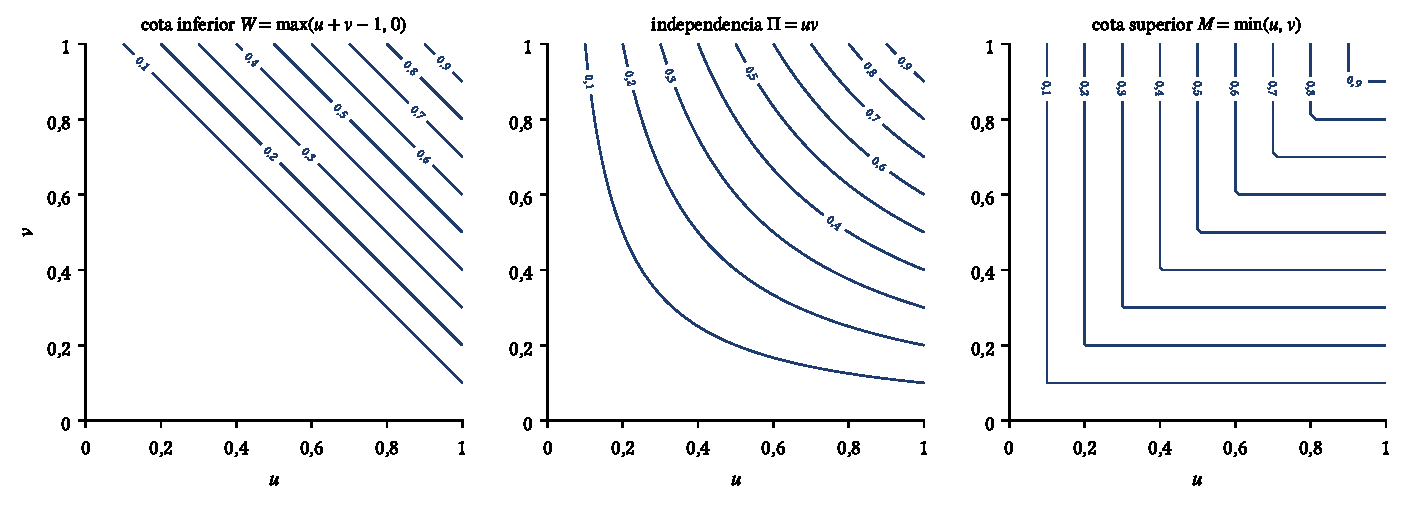
\includegraphics[width=\linewidth]{graficos/cap18_fig_frechet.pdf}
\caption{Curvas de nivel de las cotas de Fréchet-Hoeffding y de la cópula de independencia. Toda cópula está entre la
primera y la tercera.}
\label{fig:frechet}
\end{figure}

\paragraph{Densidad y verosimilitud.} Si $C$ tiene densidad $c(u,v)=\partial^2C/\partial u\,\partial v$, derivando
$H(x,y)=C(F(x),G(y))$ por la regla de la cadena,
\[
  h(x,y)=c\bigl(F(x),G(y)\bigr)\,f(x)\,g(y),\qquad
  \ln h=\ln c\bigl(F(x),G(y)\bigr)+\ln f(x)+\ln g(y).
\]
La log-verosimilitud se separa en una parte de la cópula y otra de cada margen.

% ---------------------------------------------------------------------
\section{Familias de cópulas}
% ---------------------------------------------------------------------

\paragraph{Cópulas elípticas.} La cópula gaussiana con correlación $\rho$ es la de una normal bivariada:
$C(u,v)=\Phi_2\bigl(\Phi^{-1}(u),\Phi^{-1}(v);\rho\bigr)$. La cópula $t$ es la de una $t$ bivariada con $\nu$ grados de
libertad.

\begin{proposicion}[Densidad de la cópula gaussiana]\label{prop:densgauss}
Con $x=\Phi^{-1}(u)$ e $y=\Phi^{-1}(v)$,
\[
  c(u,v)=\frac{1}{\sqrt{1-\rho^2}}\exp\Bigl(-\frac{\rho^2(x^2+y^2)-2\rho xy}{2(1-\rho^2)}\Bigr).
\]
\end{proposicion}

\begin{proof}
Por la descomposición de la densidad con márgenes normales,
\[
  c(u,v)=\frac{\phi_2(x,y;\rho)}{\phi(x)\,\phi(y)}:
\]
\begin{align*}
  c(u,v) &= \frac{\frac{1}{2\pi\sqrt{1-\rho^2}}\exp\bigl(-\frac{x^2-2\rho xy+y^2}{2(1-\rho^2)}\bigr)}{\frac{1}{2\pi}\exp\bigl(-\frac{x^2+y^2}{2}\bigr)}\\
         &= \frac{1}{\sqrt{1-\rho^2}}\exp\Bigl(-\frac{x^2-2\rho xy+y^2}{2(1-\rho^2)}+\frac{(1-\rho^2)(x^2+y^2)}{2(1-\rho^2)}\Bigr)\\
         &= \frac{1}{\sqrt{1-\rho^2}}\exp\Bigl(-\frac{\rho^2(x^2+y^2)-2\rho xy}{2(1-\rho^2)}\Bigr).
\end{align*}
\end{proof}

\paragraph{Cópulas arquimedianas.} Se construyen con un \emph{generador} $\varphi$ continuo, decreciente y convexo con
$\varphi(1)=0$: $C(u,v)=\varphi^{-1}\bigl(\varphi(u)+\varphi(v)\bigr)$. Las dos más usadas en finanzas son
\begin{itemize}[leftmargin=*]
  \item \textbf{Clayton}: $\varphi(t)=(t^{-\theta}-1)/\theta$, $\theta>0$, de modo que $C(u,v)=(u^{-\theta}+v^{-\theta}-1)^{-1/\theta}$;
  \item \textbf{Gumbel}: $\varphi(t)=(-\ln t)^\theta$, $\theta\ge1$, de modo que
        $C(u,v)=\exp\bigl\{-[(-\ln u)^\theta+(-\ln v)^\theta]^{1/\theta}\bigr\}$.
\end{itemize}

\paragraph{Medidas de concordancia.} El tau de Kendall es la probabilidad de que dos pares independientes sean
concordantes menos la de que sean discordantes; el rho de Spearman es la correlación de Pearson de $(U,V)$. Ambas
dependen solo de la cópula: $\tau=4\E[C(U,V)]-1$ y $\rho_S=12\iint C(u,v)\,du\,dv-3$. Para las cópulas elípticas,
$\tau=\frac2\pi\arcsin\rho$ (Lindskog, McNeil y Schmock, 2003), y para las arquimedianas, $\tau=1+4\int_0^1\varphi(t)/\varphi'(t)\,dt$
(Genest y MacKay, 1986).

\begin{proposicion}[Tau de Kendall de Clayton y de Gumbel]\label{prop:taukendall}
Para Clayton, $\tau=\theta/(\theta+2)$; para Gumbel, $\tau=1-1/\theta$.
\end{proposicion}

\begin{proof}
Clayton: $\varphi'(t)=-t^{-\theta-1}$, de modo que
\begin{align*}
  \frac{\varphi(t)}{\varphi'(t)} &= -\frac{(t^{-\theta}-1)\,t^{\theta+1}}{\theta}\\
                                 &= -\frac{t-t^{\theta+1}}{\theta},\\
  \int_0^1\frac{\varphi(t)}{\varphi'(t)}\,dt &= -\frac1\theta\Bigl(\frac12-\frac1{\theta+2}\Bigr)\\
                                             &= -\frac1\theta\cdot\frac{\theta}{2(\theta+2)}\\
                                             &= -\frac{1}{2(\theta+2)},\\
  \tau &= 1-\frac{4}{2(\theta+2)}\\
       &= \frac{\theta}{\theta+2}.
\end{align*}
Gumbel: $\varphi'(t)=-\theta(-\ln t)^{\theta-1}/t$, de modo que
\begin{align*}
  \frac{\varphi(t)}{\varphi'(t)} &= -\frac{t\,(-\ln t)^\theta}{\theta(-\ln t)^{\theta-1}}\\
                                 &= \frac{t\ln t}{\theta},\\
  \int_0^1t\ln t\,dt &= \Bigl[\frac{t^2\ln t}{2}\Bigr]_0^1-\int_0^1\frac t2\,dt\\
                     &= 0-\frac14,\\
  \tau &= 1+\frac4\theta\Bigl(-\frac14\Bigr)\\
       &= 1-\frac1\theta .
\end{align*}
\end{proof}

\paragraph{Dependencia en las colas.} Los coeficientes de dependencia en la cola inferior y superior son
\[
  \lambda_L=\lim_{q\to0^+}\Pr(V\le q\mid U\le q)=\lim_{q\to0^+}\frac{C(q,q)}{q},\qquad
  \lambda_U=\lim_{q\to1^-}\Pr(V>q\mid U>q).
\]
Miden la probabilidad de que un activo tenga un día extremo dado que el otro lo tuvo.

\begin{proposicion}[Dependencia en las colas de Clayton y de Gumbel]\label{prop:colas}
Clayton: $\lambda_L=2^{-1/\theta}$ y $\lambda_U=0$. Gumbel: $\lambda_L=0$ y $\lambda_U=2-2^{1/\theta}$.
\end{proposicion}

\begin{proof}
Clayton, cola inferior:
\begin{align*}
  \frac{C(q,q)}{q} &= \frac{(2q^{-\theta}-1)^{-1/\theta}}{q}\\
                   &= \bigl[q^{\theta}(2q^{-\theta}-1)\bigr]^{-1/\theta}\\
                   &= (2-q^{\theta})^{-1/\theta}\ \longrightarrow\ 2^{-1/\theta}\quad(q\to0).
\end{align*}
Gumbel, cola superior: en la diagonal,
\begin{align*}
  C(q,q) &= \exp\bigl\{-[2(-\ln q)^\theta]^{1/\theta}\bigr\}\\
         &= \exp\bigl\{2^{1/\theta}\ln q\bigr\}\\
         &= q^{2^{1/\theta}} .
\end{align*}
Por inclusión-exclusión, $\Pr(U>q,V>q)=1-2q+C(q,q)$, y con la regla de L'Hôpital:
\begin{align*}
  \lambda_U &= \lim_{q\to1}\frac{1-2q+q^{2^{1/\theta}}}{1-q}\\
            &= \lim_{q\to1}\frac{-2+2^{1/\theta}q^{2^{1/\theta}-1}}{-1}\\
            &= 2-2^{1/\theta}.
\end{align*}
Las colas opuestas son cero por cálculos análogos.
\end{proof}

La cópula gaussiana tiene $\lambda_L=\lambda_U=0$ para todo $\rho<1$: los extremos son asintóticamente independientes. La
$t$ tiene $\lambda_L=\lambda_U=2\,t_{\nu+1}\bigl(-\sqrt{(\nu+1)(1-\rho)/(1+\rho)}\bigr)$, positivo y creciente en $\rho$ y
decreciente en $\nu$ (Demarta y McNeil, 2005). La Figura~\ref{fig:copulas} compara las cuatro con el mismo $\tau=0{,}5$: la
gaussiana es simétrica y sin colas, la $t$ (con $\nu=4$, $\lambda=0{,}397$) concentra puntos en ambas esquinas, Clayton en la
inferior ($\lambda_L=0{,}707$) y Gumbel en la superior ($\lambda_U=0{,}586$).

\begin{figure}[ht]
\centering
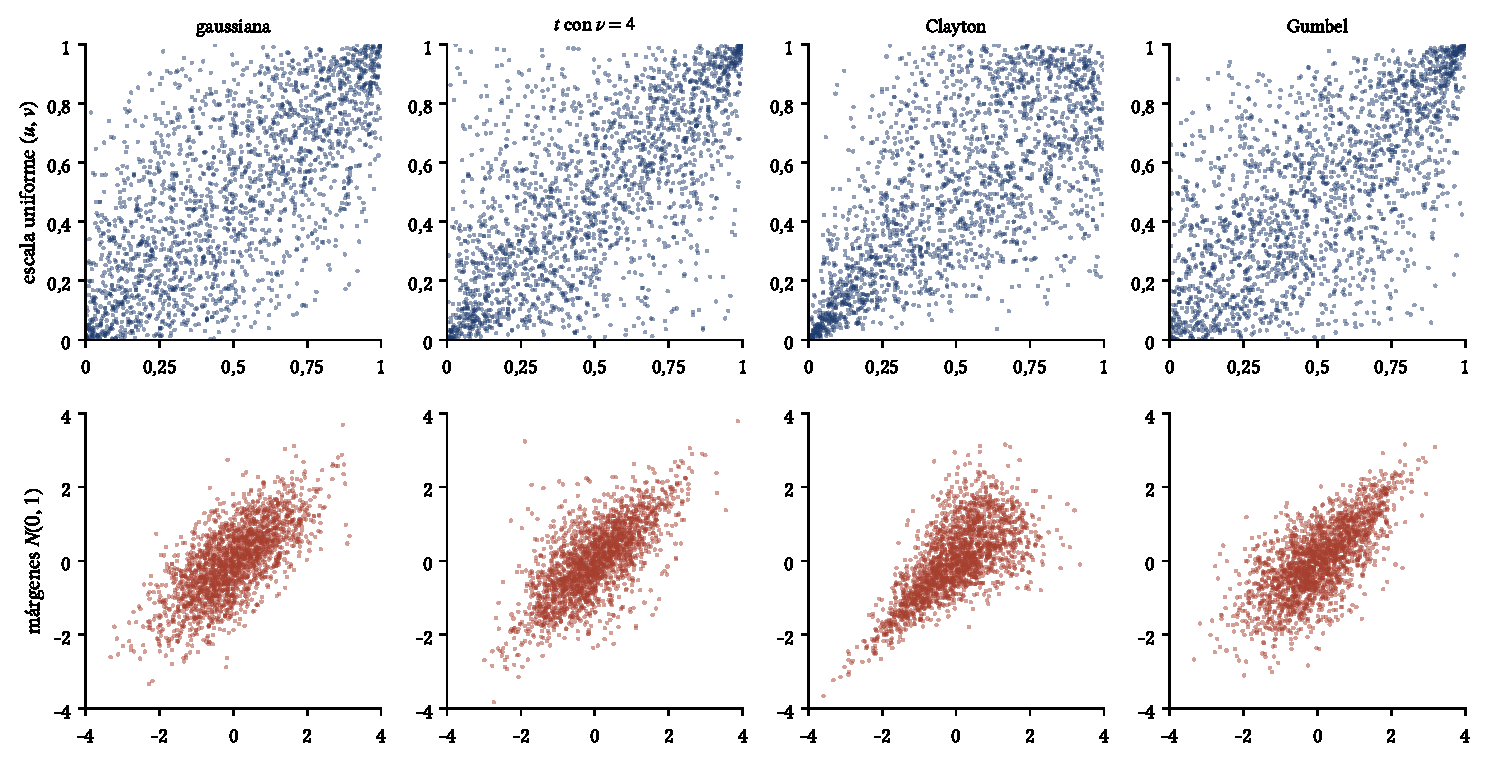
\includegraphics[width=\linewidth]{graficos/cap18_fig_copulas.pdf}
\caption{2\,000 simulaciones de cuatro cópulas con $\tau=0{,}5$ ($\rho=0{,}707$ en la gaussiana y la $t$; $\theta=2$ en Clayton y
Gumbel). Arriba, en escala uniforme; abajo, con márgenes normales, donde las diferencias en las colas se ven mejor.}
\label{fig:copulas}
\end{figure}

% ---------------------------------------------------------------------
\section{Estimación y simulación}
% ---------------------------------------------------------------------

\paragraph{Máxima verosimilitud canónica.} Como la log-verosimilitud se separa, la cópula puede estimarse sin especificar
las márgenes, sustituyéndolas por las distribuciones empíricas. Se calculan las \emph{pseudo-observaciones}
\[
  \hat u_t=\frac{\operatorname{rango}(x_t)}{n+1},\qquad \hat v_t=\frac{\operatorname{rango}(y_t)}{n+1},
\]
y se maximiza $\sum_t\ln c(\hat u_t,\hat v_t;\boldsymbol\theta)$ (Genest, Ghoudi y Rivest, 1995). Se divide entre $n+1$ y no
entre $n$ para que ningún valor sea exactamente 1, donde $\Phi^{-1}$ o $\ln(1-u)$ divergen. Si las márgenes se estiman por
separado con un modelo paramétrico y luego se estima la cópula, el método se llama de \emph{inferencia por márgenes}
(IFM; Joe, 1997). Una alternativa más simple es el \emph{método de momentos}: invertir el tau de Kendall muestral con las
fórmulas de la Proposición~\ref{prop:taukendall}.

\begin{observacion}
Las cópulas describen la dependencia de variables i.i.d. Los rendimientos diarios no lo son: su volatilidad cambia. Lo
correcto es filtrar cada serie con un modelo de volatilidad (GARCH, EWMA) y estimar la cópula de los residuos
estandarizados (el enfoque \emph{cópula-GARCH}; Patton, 2006). El Ejercicio~\ref{ej:copres} compara ambos enfoques.
\end{observacion}

\paragraph{Simulación por el método condicional.} Para simular $(U,V)$ de una cópula, se simula $U$ uniforme y luego $V$ de
la distribución condicional $C(v\mid u)=\partial C(u,v)/\partial u$, invirtiéndola en otra uniforme $W$.

\begin{proposicion}[Simulación de la cópula de Clayton]\label{prop:simclayton}
Si $U,W$ son uniformes independientes, $V=\bigl[(W^{-\theta/(1+\theta)}-1)U^{-\theta}+1\bigr]^{-1/\theta}$ tiene, junto con $U$, la
cópula de Clayton.
\end{proposicion}

\begin{proof}
La distribución condicional es la derivada parcial respecto de $u$:
\begin{align*}
  C(v\mid u) &= \frac{\partial}{\partial u}(u^{-\theta}+v^{-\theta}-1)^{-1/\theta}\\
             &= -\frac1\theta(u^{-\theta}+v^{-\theta}-1)^{-1/\theta-1}\cdot(-\theta u^{-\theta-1})\\
             &= u^{-\theta-1}(u^{-\theta}+v^{-\theta}-1)^{-(1+\theta)/\theta}.
\end{align*}
Igualamos a $w$ y despejamos $v$:
\begin{align*}
  (u^{-\theta}+v^{-\theta}-1)^{-(1+\theta)/\theta} &= w\,u^{\theta+1}\\
  u^{-\theta}+v^{-\theta}-1 &= w^{-\theta/(1+\theta)}u^{-\theta}\\
  v^{-\theta} &= (w^{-\theta/(1+\theta)}-1)u^{-\theta}+1\\
  v &= \bigl[(w^{-\theta/(1+\theta)}-1)u^{-\theta}+1\bigr]^{-1/\theta}.
\end{align*}
Como $W=C(V\mid U)$ es uniforme e independiente de $U$, el par simulado tiene la distribución condicional correcta.
\end{proof}

Para la gaussiana se simulan normales correlacionadas y se aplica $\Phi$; para la $t$, además, se divide entre
$\sqrt{W/\nu}$ con $W\sim\chi^2_\nu$ y se aplica $t_\nu$. Para Gumbel se usa el algoritmo de Marshall y Olkin (1988):
$U_i=\exp\{-(E_i/S)^{1/\theta}\}$, con $E_i$ exponenciales y $S$ una variable estable positiva de índice $1/\theta$.

% ---------------------------------------------------------------------
\section{Ejercicios resueltos}
% ---------------------------------------------------------------------

\begin{ejresuelto}{Medidas de dependencia del S\&P 500 y el Nasdaq}\label{ej:medidas}
\enunciado Describa los dos índices, calcule las correlaciones de Pearson, Kendall y Spearman, y estime la dependencia en las
colas con $\hat\lambda_L(q)=\#\{\hat u_t\le q,\hat v_t\le q\}/(nq)$ y su análogo superior para $q=10$, 5 y 1\,\%. Compare con lo
que implicaría una cópula gaussiana con el mismo tau.

\solucion
\paso{Paso 1. Márgenes.} Ambos índices tienen colas muy pesadas: curtosis 11,17 (S\&P 500) y 8,43 (Nasdaq), con volatilidades
diarias de 1,20 y 1,59\,\%.

\paso{Paso 2. Correlaciones.} Pearson $=0{,}8872$, Kendall $=0{,}7348$ y Spearman $=0{,}8919$. Si la cópula fuera gaussiana, el tau
implicaría
\begin{align*}
  \rho &= \sin\Bigl(\frac{\pi\times0{,}7348}{2}\Bigr)\\
       &= \sin(1{,}1542)\\
       &= 0{,}9145,
\end{align*}
mayor que la correlación de Pearson de los rendimientos: las colas pesadas de las márgenes reducen la correlación lineal.

\paso{Paso 3. Colas.}
\begin{center}\small
\begin{tabular}{@{}rrrr@{}}
\toprule
$q$ & $\hat\lambda_L(q)$ & $\hat\lambda_U(q)$ & Gaussiana con $\rho=0{,}9145$ \\
\midrule
10\,\% & 0,742 & 0,720 & 0,712 \\
5\,\% & 0,620 & 0,700 & 0,664 \\
1\,\% & 0,457 & 0,596 & 0,574 \\
\bottomrule
\end{tabular}
\end{center}
Con $q=1$\,\%, si el S\&P 500 está entre sus 50 peores días, el Nasdaq también lo está en el 45,7\,\% de los casos. La
gaussiana predice que esa probabilidad cae hacia cero cuando $q\to0$, pero lo hace lentamente con $\rho=0{,}91$. Los cinco peores
días del S\&P 500 fueron en septiembre a diciembre de 2008, y en los tres primeros el Nasdaq tuvo uno de sus cuatro peores días
(Figura~\ref{fig:dispersion}).

\codigoweb{cap18_ej01}
\salidaR{cap18_ej01_R.txt}
\lectura{cap18_ej01}

\RvsPy El tau de Kendall se calcula con \texttt{cor(..., method = "kendall")} en R y con \texttt{scipy.stats.kendalltau} en
Python; ambos dan la versión $\tau_b$, corregida por empates. Los rangos promedio de \texttt{rank} y \texttt{rankdata}
coinciden. La probabilidad de la normal bivariada en la diagonal, $\Phi_2(a,a;\rho)=\int_{-\infty}^a\phi(x)\Phi\bigl((a-\rho
x)/\sqrt{1-\rho^2}\bigr)dx$, se integra con la regla de Simpson en ambos lenguajes para no depender de paquetes externos
(\texttt{mvtnorm} en R).

\begin{figure}[ht]
\centering
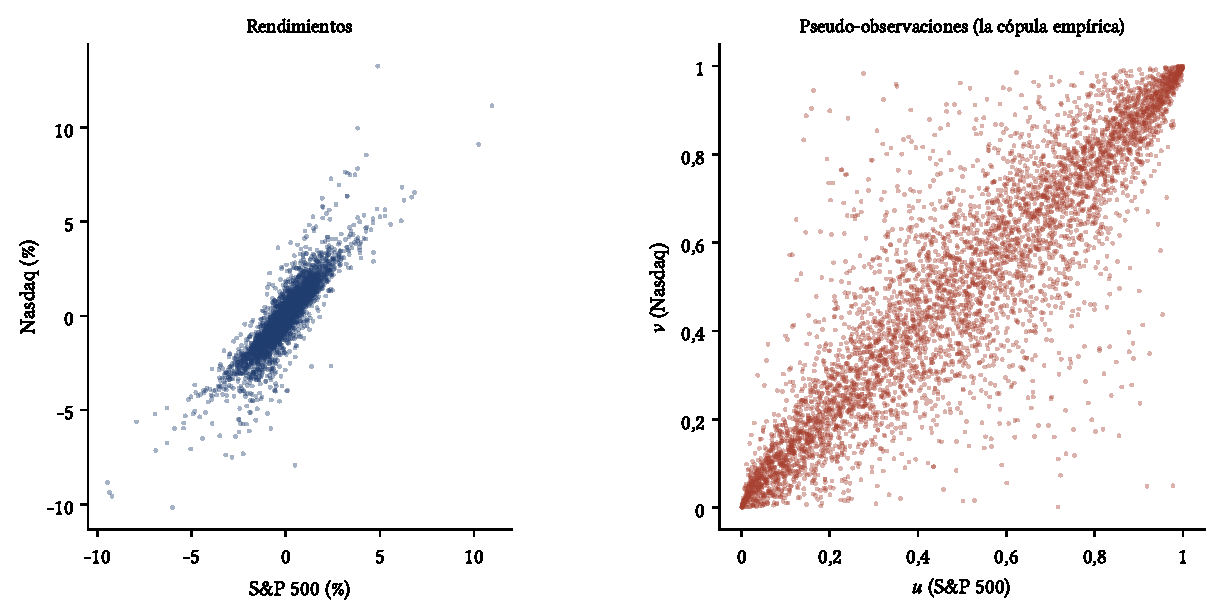
\includegraphics[width=\linewidth]{graficos/cap18_ej01_dispersion.pdf}
\caption{Izquierda: rendimientos diarios del S\&P 500 y el Nasdaq. Derecha: sus pseudo-observaciones, que eliminan el efecto de
las márgenes y muestran solo la cópula.}
\label{fig:dispersion}
\end{figure}

\begin{conclusion}
Los dos índices están muy correlacionados y su dependencia en las colas es alta, aunque con este nivel de correlación la
gaussiana se acerca a los valores empíricos hasta $q=1$\,\%. Para decidir qué cópula usar hay que estimarlas.
\end{conclusion}
\end{ejresuelto}

\begin{ejresuelto}{Estimación de cuatro cópulas}\label{ej:cuatro}
\enunciado Estime por máxima verosimilitud canónica las cópulas gaussiana, $t$, Clayton y Gumbel para los rendimientos.
Compare con AIC y con las medidas implícitas de dependencia.

\solucion
\paso{Paso 1. Resultados.}
\begin{center}\small
\begin{tabular}{@{}llrrrrr@{}}
\toprule
Cópula & Parámetros & $\ell$ & AIC & $\tau$ & $\lambda_L$ & $\lambda_U$ \\
\midrule
Gaussiana & $\rho=0{,}9008$ & 4\,189,57 & $-8\,377{,}14$ & 0,714 & 0 & 0 \\
$t$ & $\rho=0{,}9122$, $\nu=3{,}62$ & 4\,539,52 & $-9\,075{,}04$ & 0,731 & 0,666 & 0,666 \\
Clayton & $\theta=3{,}3756$ & 3\,447,99 & $-6\,893{,}97$ & 0,628 & 0,814 & 0 \\
Gumbel & $\theta=3{,}5190$ & 4\,258,52 & $-8\,515{,}04$ & 0,716 & 0 & 0,782 \\
\bottomrule
\end{tabular}
\end{center}
La cópula $t$ gana con claridad: mejora la log-verosimilitud de la gaussiana en 350 puntos con un solo parámetro más. Su
$\tau$ implícito, 0,731, es el más cercano al empírico (0,735).

\paso{Paso 2. Interpretación de $\nu$.} Para la gaussiana,
\begin{align*}
  \tau &= \frac2\pi\arcsin(0{,}9008)\\
       &= 0{,}6366\times1{,}1217\\
       &= 0{,}714 .
\end{align*}
Que $\hat\nu=3{,}62$ sea tan bajo indica dependencia fuerte en ambas colas. Clayton, que solo tiene cola inferior, es la peor:
estos datos tienen tanta dependencia en la cola superior como en la inferior. Gumbel, con su cola superior, queda segunda.

\paso{Paso 3. Momentos frente a verosimilitud.} Invirtiendo el tau empírico se obtiene $\theta=5{,}54$ para Clayton y $3{,}77$
para Gumbel, lejos de los estimadores de máxima verosimilitud (3,38 y 3,52). Cuando la familia está mal especificada, los dos
métodos estiman cosas distintas: el de momentos reproduce el tau; el de verosimilitud, la forma global de la densidad
(Figura~\ref{fig:contornos}).

\codigoweb{cap18_ej02}
\salidaR{cap18_ej02_R.txt}
\lectura{cap18_ej02}

\RvsPy Para que ambos lenguajes den los mismos parámetros, no usamos los optimizadores de cada uno (\texttt{optim},
\texttt{scipy.optimize}), que difieren en sus criterios de parada, sino una búsqueda de la sección áurea programada igual en
los dos. La cópula $t$ se estima por perfil: para cada $\nu$ de 2 a 30 se maximiza en $\rho$, y luego se refina $\nu$ con otra
búsqueda áurea. Las densidades de Clayton y de Gumbel se verificaron contra la segunda derivada numérica de $C$, y la de la $t$
contra \texttt{scipy.stats.multivariate\_t}. Los paquetes \texttt{copula} (R) y \texttt{copulae} (Python) hacen esto
automáticamente.

\begin{figure}[ht]
\centering
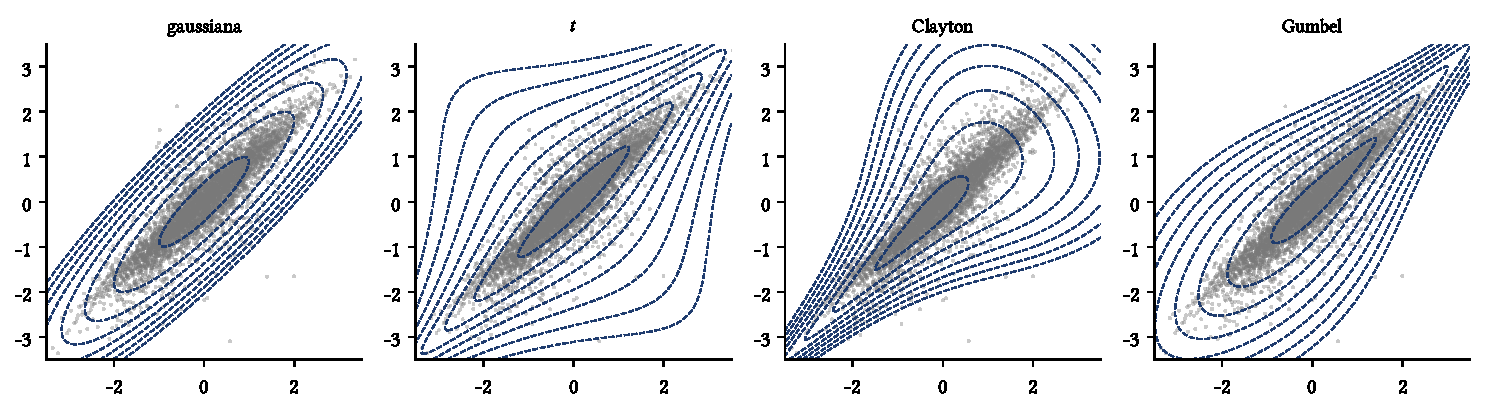
\includegraphics[width=\linewidth]{graficos/cap18_ej02_contornos.pdf}
\caption{Curvas de nivel de las cuatro cópulas estimadas con márgenes normales, sobre las pseudo-observaciones transformadas
$(\Phi^{-1}(\hat u),\Phi^{-1}(\hat v))$.}
\label{fig:contornos}
\end{figure}

\begin{conclusion}
La cópula $t$ con pocos grados de libertad es la que mejor describe la dependencia diaria entre los dos índices: alta
correlación y dependencia simétrica en ambas colas.
\end{conclusion}
\end{ejresuelto}

\begin{ejresuelto}{La cópula de los residuos estandarizados}\label{ej:copres}
\enunciado Estandarice cada rendimiento con una volatilidad EWMA ($\lambda=0{,}94$) y repita la estimación con los residuos.
Compare la dependencia en las colas antes y después de filtrar la volatilidad.

\solucion
\paso{Paso 1. Efecto del filtro.} La curtosis baja de 11,17 a 6,01 (S\&P 500) y de 8,43 a 4,55 (Nasdaq), y el tau sube de 0,735 a
0,745. La correlación de Pearson sube aún más, de 0,887 a 0,921, porque los residuos tienen colas menos pesadas.

\paso{Paso 2. Colas empíricas.}
\begin{center}\small
\begin{tabular}{@{}lrrrrrr@{}}
\toprule
 & \multicolumn{3}{c}{$\hat\lambda_L(q)$} & \multicolumn{3}{c}{$\hat\lambda_U(q)$} \\
\cmidrule(lr){2-4}\cmidrule(lr){5-7}
 & 10\,\% & 5\,\% & 1\,\% & 10\,\% & 5\,\% & 1\,\% \\
\midrule
Rendimientos & 0,742 & 0,620 & 0,457 & 0,720 & 0,700 & 0,596 \\
Residuos EWMA & 0,734 & 0,692 & 0,656 & 0,748 & 0,696 & 0,616 \\
\bottomrule
\end{tabular}
\end{center}
Con los residuos, la dependencia en la cola inferior al 1\,\% sube de 0,457 a 0,656. En los rendimientos, los días de caída más
extrema de cada índice se repartían entre episodios de alta volatilidad, en los que el otro índice también caía pero no
siempre entre sus peores días absolutos. Al dividir por la volatilidad, se comparan sorpresas relativas, que coinciden más.

\paso{Paso 3. Cópulas.} La $t$ sigue siendo la mejor, ahora con $\rho=0{,}9213$, $\nu=5{,}20$ y $\lambda=0{,}632$ (frente a
$\nu=3{,}62$ y $\lambda=0{,}666$ en los rendimientos): parte de lo que parecía dependencia en las colas era volatilidad
común. La ventaja de la $t$ sobre la gaussiana baja de 350 a 137 puntos de log-verosimilitud (Figura~\ref{fig:colas18}).

\codigoweb{cap18_ej03}
\salidaR{cap18_ej03_R.txt}
\lectura{cap18_ej03}

\RvsPy La función \texttt{ewma\_estandarizar} inicia la varianza con la media de los cuadrados de las 30 primeras observaciones;
con 5\,030 datos, el valor inicial casi no influye. Se usa el mismo filtro que en el Capítulo~\ref{cap:dcc}.

\begin{figure}[ht]
\centering
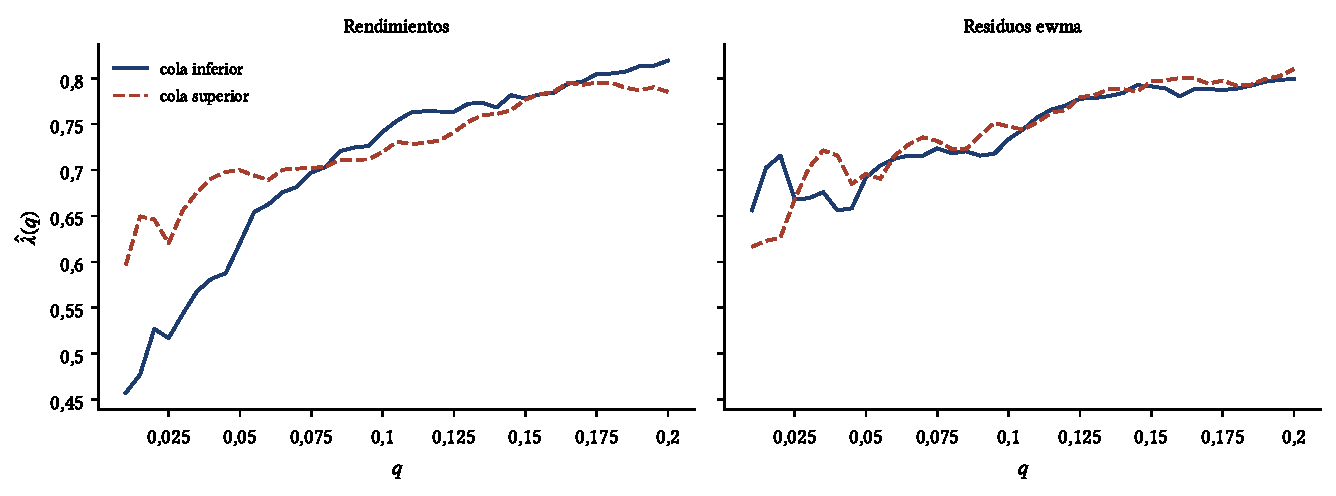
\includegraphics[width=0.9\linewidth]{graficos/cap18_ej03_colas.pdf}
\caption{Dependencia empírica en las colas $\hat\lambda(q)$ en función de $q$, para los rendimientos y para los residuos
estandarizados.}
\label{fig:colas18}
\end{figure}

\begin{conclusion}
La cópula de los rendimientos mezcla la dependencia de las sorpresas con la de las volatilidades. Filtrar primero la
volatilidad da una cópula más estable y con una interpretación más limpia, que es la que se usa para simular.
\end{conclusion}
\end{ejresuelto}

\begin{ejresuelto}{Riesgo de una cartera con cópulas}\label{ej:cartera18}
\enunciado Para una cartera con 50\,\% en cada índice, simule 20\,000 escenarios del día siguiente al 31 de diciembre de 2018
con cada cópula de los residuos, márgenes empíricas de los residuos y la volatilidad EWMA pronosticada. Calcule el VaR y el ES
al 99\,\% y compare con la independencia, la comonotonía y la simulación histórica filtrada.

\solucion
\paso{Paso 1. Escenarios.} Cada escenario es $L=-(0{,}5\,\hat\sigma_x\hat F_x^{-1}(U)+0{,}5\,\hat\sigma_y\hat F_y^{-1}(V))$, con
$(U,V)$ de la cópula, $\hat F^{-1}$ el cuantil empírico de los residuos y $\hat\sigma_x=1{,}764$\,\%, $\hat\sigma_y=2{,}102$\,\%.

\paso{Paso 2. Resultados} (pérdidas en \%).
\begin{center}\small
\begin{tabular}{@{}lrrrr@{}}
\toprule
Cópula & $\tau$ simulado & VaR 99\,\% & ES 99\,\% & VaR 99,9\,\% \\
\midrule
Gaussiana & 0,753 & 5,13 & 6,63 & 8,87 \\
$t$ & 0,760 & 5,17 & 6,66 & 8,88 \\
Clayton & 0,668 & 5,23 & 6,77 & 9,22 \\
Gumbel & 0,717 & 5,01 & 6,35 & 8,29 \\
Independencia & 0,021 & 3,68 & 4,63 & 5,76 \\
Comonotonía & 1,000 & 5,27 & 6,81 & 9,66 \\
Histórica filtrada & -- & 5,29 & 6,96 & 9,96 \\
\bottomrule
\end{tabular}
\end{center}
Con dependencia tan alta, las cuatro cópulas dan VaR al 99\,\% entre 5,0 y 5,2\,\%, cerca del de la comonotonía. Suponer
independencia subestimaría el VaR en casi un tercio:
\begin{align*}
  1-\frac{3{,}68}{5{,}17} &= 1-0{,}712\\
                         &= 0{,}288 .
\end{align*}
Clayton, con más dependencia en la cola inferior (la de las pérdidas), da el VaR al 99,9\,\% más alto; Gumbel, cuya
dependencia está en las ganancias, el más bajo.

\paso{Paso 3. La cota comonótona.} Como el ES es subaditivo, el ES de la cartera no puede superar el promedio ponderado de los ES
de cada índice, que es el ES comonótono. Con los 5\,030 residuos observados, esa cota es 7,10\,\% y el ES histórico, 6,96\,\%: la
diversificación ahorra apenas 0,13 puntos. El ES comonótono simulado (6,81) queda por debajo del histórico por el error de
simulación en la cola extrema: con 20\,000 escenarios, el ES al 99\,\% promedia solo 200 de ellos (Figura~\ref{fig:cartera18}).

\codigoweb{cap18_ej04}
\salidaR{cap18_ej04_R.txt}
\lectura{cap18_ej04}

\RvsPy Las uniformes salen del generador de Park y Miller del Capítulo~\ref{cap:eventos}, y las normales, las $\chi^2$ y las $t$
se obtienen por inversión (\texttt{qnorm}, \texttt{qchisq}, \texttt{pt} y sus equivalentes de \texttt{scipy.stats}), de modo
que R y Python simulan los mismos escenarios. Los cuantiles empíricos usan la interpolación por omisión de \texttt{quantile} y
\texttt{np.quantile}, que es la misma (tipo 7).

\begin{figure}[ht]
\centering
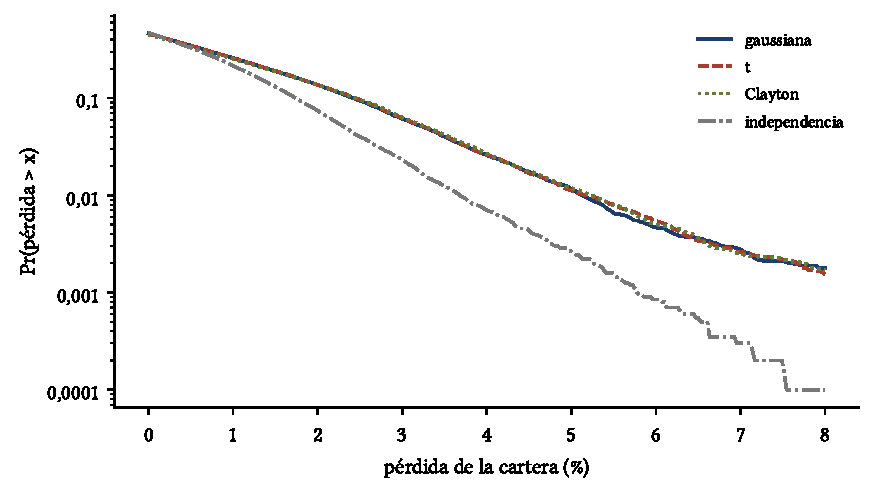
\includegraphics[width=0.78\linewidth]{graficos/cap18_ej04_colas_cartera.pdf}
\caption{Probabilidad de que la pérdida diaria de la cartera supere $x$, en escala logarítmica, según la cópula usada en la
simulación.}
\label{fig:cartera18}
\end{figure}

\begin{conclusion}
La elección de la cópula importa poco cuando los activos están casi perfectamente correlacionados, y mucho cuando se comparan
supuestos extremos como la independencia. En carteras de activos menos correlacionados (acciones y bonos, distintos países),
la diferencia entre la gaussiana y la $t$ en el VaR al 99,9\,\% es mucho mayor.
\end{conclusion}
\end{ejresuelto}

\begin{ejresuelto}{Dependencia en las crisis}\label{ej:crisis18}
\enunciado Separe la crisis financiera (julio de 2007 a junio de 2009) del resto de la muestra y estime las cópulas de los
residuos en cada parte. Calcule además el tau de Kendall en ventanas móviles de 250 días.

\solucion
\paso{Paso 1. Medidas empíricas.}
\begin{center}\small
\begin{tabular}{@{}lrrrrr@{}}
\toprule
Muestra & Días & Pearson & $\tau$ & $\hat\lambda_L$ (5\,\%) & $\hat\lambda_U$ (5\,\%) \\
\midrule
Crisis & 504 & 0,953 & 0,799 & 0,833 & 0,794 \\
Resto & 4\,526 & 0,917 & 0,740 & 0,685 & 0,681 \\
\bottomrule
\end{tabular}
\end{center}
En la crisis, la dependencia sube en todas las medidas, y más en la cola inferior.

\paso{Paso 2. Cópulas.} En la crisis, la $t$ estima $\rho=0{,}950$ y $\nu=4{,}33$, con $\lambda=0{,}727$; en el resto, $\rho=0{,}918$,
$\nu=5{,}37$ y $\lambda=0{,}619$. En ambas submuestras la $t$ tiene la mayor verosimilitud.

\paso{Paso 3. Evolución.} El tau móvil va de 0,585 (ventana que termina en agosto de 2000, en plena burbuja tecnológica) a 0,832 (ventana que termina en septiembre de 2009), con mediana 0,751
(Figura~\ref{fig:taumovil}).

\codigoweb{cap18_ej05}
\salidaR{cap18_ej05_R.txt}
\lectura{cap18_ej05}

\RvsPy Las pseudo-observaciones se recalculan dentro de cada submuestra, para que sean uniformes en ella. El tau móvil usa 228
ventanas; en R, \texttt{sapply} sobre los índices de inicio, y en Python, una comprensión de listas.

\begin{figure}[ht]
\centering
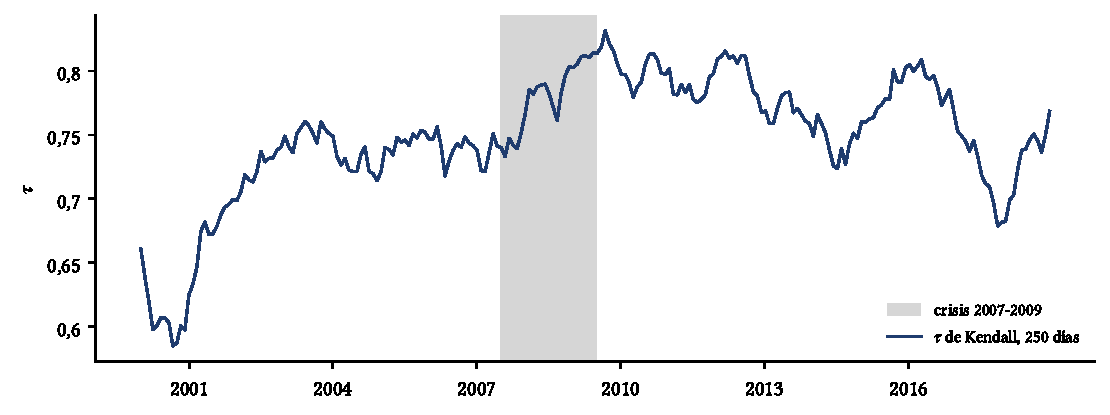
\includegraphics[width=\linewidth]{graficos/cap18_ej05_tau_movil.pdf}
\caption{Tau de Kendall de los residuos en ventanas de 250 días, fechado al final de cada ventana. En gris, la crisis de 2007--2009.}
\label{fig:taumovil}
\end{figure}

\begin{conclusion}
La dependencia no es constante: aumenta en las crisis, justo cuando la diversificación más se necesita. Una cópula estimada
con toda la muestra subestima el riesgo conjunto en esos períodos; las cópulas dinámicas (Patton, 2006) y los modelos DCC del
Capítulo~\ref{cap:dcc} abordan este problema.
\end{conclusion}
\end{ejresuelto}

% ---------------------------------------------------------------------
\section{Ejercicios propuestos}
% ---------------------------------------------------------------------

\begin{enumerate}[label=\textbf{\thechapter.\arabic*},leftmargin=*,itemsep=6pt]
  \item Para $\tau=0{,}4$, calcule el parámetro de las cópulas gaussiana, Clayton y Gumbel, y la dependencia en las colas de
  las dos últimas. \textit{Respuesta: $\rho=0{,}5878$; $\theta=1{,}333$ y $1{,}667$; $\lambda_L=0{,}5946$ y $\lambda_U=0{,}4843$.}

  \item Calcule la dependencia en las colas de una cópula $t$ con $\rho=0{,}5$ y $\nu=4$. \textit{Respuesta: $2\,t_5(-1{,}291)=0{,}2532$.}

  \item Si $X\sim N(0,1)$ e $Y=e^X$, demuestre que $\operatorname{Corr}(X,Y)=1/\sqrt{e-1}=0{,}763$, aunque la cópula es la comonotónica y
  $\tau=1$.

  \item Demuestre que la cópula de $(X,-Y)$ es $C^*(u,v)=u-C(u,1-v)$ y que su tau de Kendall es $-\tau$.

  \item Demuestre que la cópula de Clayton tiende a la de independencia cuando $\theta\to0$ y a la comonotónica cuando
  $\theta\to\infty$.

  \item \emph{(Simulación.)} Simule 500 muestras de $n=1\,000$ de una cópula $t$ con $\rho=0{,}7$ y $\nu=4$, y estime en cada una la
  gaussiana y la $t$. ¿En qué porcentaje de muestras gana la $t$ por AIC? ¿Cuál es el sesgo de $\hat\nu$?

  \item \emph{(Con datos de la BVL.)} Estime la cópula entre los rendimientos diarios del índice S\&P/BVL Perú General y del
  precio del cobre. ¿Hay más dependencia en las caídas que en las subidas?

  \item \emph{(Con datos.)} Con los precios de Apple y Alphabet del Capítulo~\ref{cap:eventos}, repita los
  Ejercicios~\ref{ej:cuatro} y \ref{ej:copres}. ¿Es la dependencia entre dos acciones del mismo sector parecida a la de dos índices?
\end{enumerate}

% ---------------------------------------------------------------------
\section{Resumen de fórmulas}
% ---------------------------------------------------------------------

\begin{table}[H]
\centering\small
\begin{tabular}{@{}ll@{}}
\toprule
Concepto & Fórmula \\
\midrule
Sklar & $H(x,y)=C(F(x),G(y))$;\quad $h=c(F,G)\,f\,g$ \\
Fréchet-Hoeffding & $\max(u+v-1,0)\le C(u,v)\le\min(u,v)$ \\
Gaussiana & $c=\frac{1}{\sqrt{1-\rho^2}}\exp\bigl(-\frac{\rho^2(x^2+y^2)-2\rho xy}{2(1-\rho^2)}\bigr)$;\quad $\tau=\frac2\pi\arcsin\rho$;\quad $\lambda=0$ \\
$t$ & $\tau=\frac2\pi\arcsin\rho$;\quad $\lambda_L=\lambda_U=2t_{\nu+1}\bigl(-\sqrt{(\nu+1)(1-\rho)/(1+\rho)}\bigr)$ \\
Clayton & $C=(u^{-\theta}+v^{-\theta}-1)^{-1/\theta}$;\quad $\tau=\frac{\theta}{\theta+2}$;\quad $\lambda_L=2^{-1/\theta}$ \\
Gumbel & $C=\exp\{-[(-\ln u)^\theta+(-\ln v)^\theta]^{1/\theta}\}$;\quad $\tau=1-\frac1\theta$;\quad $\lambda_U=2-2^{1/\theta}$ \\
Pseudo-observaciones & $\hat u_t=\operatorname{rango}(x_t)/(n+1)$ \\
Cola empírica & $\hat\lambda_L(q)=\#\{\hat u_t\le q,\hat v_t\le q\}/(nq)$ \\
\bottomrule
\end{tabular}
\caption{Fórmulas principales del Capítulo 18.}
\end{table}

\section*{Referencias}
\begin{itemize}[leftmargin=*]
  \item Demarta, S. y McNeil, A. J. (2005). The $t$ copula and related copulas. \emph{International Statistical Review}, 73(1),
        111--129.
  \item Embrechts, P., McNeil, A. J. y Straumann, D. (2002). Correlation and dependence in risk management: Properties and
        pitfalls. En M. Dempster (ed.), \emph{Risk Management: Value at Risk and Beyond}, 176--223. Cambridge University Press.
  \item Genest, C., Ghoudi, K. y Rivest, L.-P. (1995). A semiparametric estimation procedure of dependence parameters in
        multivariate families of distributions. \emph{Biometrika}, 82(3), 543--552.
  \item Genest, C. y MacKay, J. (1986). The joy of copulas: Bivariate distributions with uniform marginals. \emph{The American
        Statistician}, 40(4), 280--283.
  \item Joe, H. (1997). \emph{Multivariate Models and Dependence Concepts}. Chapman \& Hall.
  \item Lindskog, F., McNeil, A. J. y Schmock, U. (2003). Kendall's tau for elliptical distributions. En G. Bol et al. (eds.),
        \emph{Credit Risk: Measurement, Evaluation and Management}, 149--156. Physica-Verlag.
  \item MacKenzie, D. y Spears, T. (2014). `The formula that killed Wall Street': The Gaussian copula and modelling practices
        in investment banking. \emph{Social Studies of Science}, 44(3), 393--417.
  \item Marshall, A. W. y Olkin, I. (1988). Families of multivariate distributions. \emph{Journal of the American Statistical
        Association}, 83(403), 834--841.
  \item McNeil, A. J., Frey, R. y Embrechts, P. (2015). \emph{Quantitative Risk Management}, ed. revisada, cap. 7. Princeton
        University Press.
  \item Nelsen, R. B. (2006). \emph{An Introduction to Copulas}, 2.ª ed. Springer.
  \item Patton, A. J. (2006). Modelling asymmetric exchange rate dependence. \emph{International Economic Review}, 47(2),
        527--556.
\end{itemize}

% =====================================================================
%  Capítulo 19. Datos de panel en finanzas
% =====================================================================
\chapter[Datos de panel]{Datos de panel en finanzas: efectos fijos, errores agrupados y paneles dinámicos}\label{cap:panel}

\section*{Objetivos de aprendizaje}
Al terminar este capítulo, el lector podrá:
\begin{enumerate}[label=\arabic*.,leftmargin=*]
  \item Estimar modelos de panel con MCO agrupado, efectos fijos, efectos aleatorios y primeras diferencias, y elegir
        entre ellos con la prueba de Hausman.
  \item Calcular errores estándar robustos a la correlación dentro de empresas, dentro de períodos o en ambas
        dimensiones, y saber cuál usar según la estructura de los datos (Petersen, 2009).
  \item Reconocer el sesgo de Nickell en los paneles dinámicos y corregirlo con variables instrumentales.
  \item Interpretar los efectos fijos de tiempo como una forma de aislar la variación de corte transversal, y relacionarlos
        con las regresiones de Fama y MacBeth.
\end{enumerate}

\section*{Motivación}
Buena parte de la investigación en finanzas corporativas y en valoración de activos usa paneles: muchas empresas
observadas durante muchos años, o muchas carteras observadas durante muchos meses. ¿Invierten más las empresas con
mayor valor de mercado? ¿Pagan los activos con mejor rendimiento pasado más rendimiento futuro? Un panel permite
controlar características de cada empresa que no se observan y que no cambian en el tiempo, y también choques comunes
a todas las empresas en un período. Pero los paneles financieros tienen una trampa: los residuos están correlacionados
dentro de cada empresa a lo largo del tiempo y dentro de cada período entre empresas. Petersen (2009) revisó los
artículos publicados en las tres principales revistas de finanzas y encontró que muchos ignoraban una u otra
correlación, con errores estándar subestimados.

\paragraph{Datos del capítulo.} Los datos de inversión de Grunfeld (1958): 10 grandes empresas industriales de EE.\,UU.
observadas de 1935 a 1954, con su inversión bruta, su valor de mercado y su stock de capital, en la versión de Baltagi
(2001). Y un panel de 30 carteras de Kenneth French (12 industrias, 9 de tamaño y valor y 9 de tamaño y momentum) con
807 meses, de enero de 1950 a marzo de 2017.

% ---------------------------------------------------------------------
\section{El modelo de efectos individuales}
% ---------------------------------------------------------------------

Sea $y_{it}$ la variable de la unidad $i=1,\dots,N$ en el período $t=1,\dots,T$. El modelo básico es
\[
  y_{it}=\mathbf x_{it}'\boldsymbol\beta+\alpha_i+\varepsilon_{it},
\]
donde $\alpha_i$ recoge todo lo que distingue a la unidad $i$ y no cambia en el tiempo: la calidad de la gerencia, la
tecnología del sector, la cultura de la empresa. Suponemos \emph{exogeneidad estricta}: $\E[\varepsilon_{it}\mid\mathbf
x_{i1},\dots,\mathbf x_{iT},\alpha_i]=0$. Lo que distingue a los estimadores es qué suponen sobre $\alpha_i$.

\paragraph{MCO agrupado.} Ignora $\alpha_i$ y estima por MCO con todas las observaciones. Es consistente solo si
$\alpha_i$ no está correlacionado con $\mathbf x_{it}$. Si las empresas con más valor de mercado tienen también, por
razones no observadas, más inversión, el estimador atribuye a $\mathbf x$ lo que es de $\alpha$ (Figura~\ref{fig:panelteoria}).

\paragraph{Efectos fijos (within).} Trata los $\alpha_i$ como parámetros y los elimina restando a cada variable su
media de la unidad, $\bar y_i=\frac1T\sum_ty_{it}$.

\begin{proposicion}[Estimador within]\label{prop:within}
Con $\ddot y_{it}=y_{it}-\bar y_i$ y $\ddot{\mathbf x}_{it}=\mathbf x_{it}-\bar{\mathbf x}_i$, el estimador
$\hat{\boldsymbol\beta}_W=(\sum_{i,t}\ddot{\mathbf x}_{it}\ddot{\mathbf x}_{it}')^{-1}\sum_{i,t}\ddot{\mathbf x}_{it}\ddot y_{it}$ es
insesgado bajo exogeneidad estricta, cualquiera sea la correlación entre $\alpha_i$ y $\mathbf x_{it}$.
\end{proposicion}

\begin{proof}
Promediando el modelo en el tiempo, $\bar y_i=\bar{\mathbf x}_i'\boldsymbol\beta+\alpha_i+\bar\varepsilon_i$. Restando:
\begin{align*}
  y_{it}-\bar y_i &= (\mathbf x_{it}-\bar{\mathbf x}_i)'\boldsymbol\beta+(\alpha_i-\alpha_i)+(\varepsilon_{it}-\bar\varepsilon_i)\\
  \ddot y_{it} &= \ddot{\mathbf x}_{it}'\boldsymbol\beta+\ddot\varepsilon_{it} .
\end{align*}
El efecto individual desaparece. Sustituyendo en el estimador:
\begin{align*}
  \hat{\boldsymbol\beta}_W &= \Bigl(\sum\ddot{\mathbf x}_{it}\ddot{\mathbf x}_{it}'\Bigr)^{-1}\sum\ddot{\mathbf x}_{it}(\ddot{\mathbf x}_{it}'\boldsymbol\beta+\ddot\varepsilon_{it})\\
                           &= \boldsymbol\beta+\Bigl(\sum\ddot{\mathbf x}_{it}\ddot{\mathbf x}_{it}'\Bigr)^{-1}\sum\ddot{\mathbf x}_{it}\ddot\varepsilon_{it}.
\end{align*}
Como $\ddot{\mathbf x}_{it}$ depende de $\mathbf x_{i1},\dots,\mathbf x_{iT}$ y $\ddot\varepsilon_{it}$ tiene esperanza condicional
cero dados esos valores (exogeneidad estricta), el segundo término tiene esperanza cero.
\end{proof}

El precio es que todo lo que no cambia en el tiempo desaparece junto con $\alpha_i$: no se puede estimar el efecto de una
característica fija de la empresa, y solo se usa la variación \emph{dentro} de cada unidad. Los grados de libertad para
$\hat\sigma^2_\varepsilon$ son $NT-N-K$, porque se estimaron implícitamente $N$ medias.

\paragraph{Primeras diferencias.} Otra forma de eliminar $\alpha_i$ es restar el período anterior:
$\Delta y_{it}=\Delta\mathbf x_{it}'\boldsymbol\beta+\Delta\varepsilon_{it}$. Con $T=2$, primeras diferencias y efectos fijos dan
exactamente el mismo estimador (Ejercicio propuesto 19.4); con $T>2$ difieren, y es más eficiente el within si los
$\varepsilon_{it}$ no están autocorrelacionados, y las diferencias si siguen un paseo aleatorio.

\paragraph{Efectos aleatorios.} Si se supone que $\alpha_i$ no está correlacionado con $\mathbf x_{it}$, con varianza
$\sigma_u^2$, el término compuesto $v_{it}=\alpha_i+\varepsilon_{it}$ tiene correlación $\sigma_u^2/(\sigma_u^2+\sigma_\varepsilon^2)$
entre dos períodos de la misma unidad, y el estimador eficiente es MCG.

\begin{proposicion}[Efectos aleatorios como cuasi-diferencia]\label{prop:re}
El estimador de MCG del modelo de efectos aleatorios es MCO sobre
$y_{it}-\theta\bar y_i=(1-\theta)\mu+(\mathbf x_{it}-\theta\bar{\mathbf x}_i)'\boldsymbol\beta+\text{error}$, con
\[
  \theta=1-\frac{\sigma_\varepsilon}{\sqrt{\sigma_\varepsilon^2+T\sigma_u^2}}.
\]
\end{proposicion}

\begin{proof}
Para la unidad $i$, la covarianza de $\mathbf v_i=(v_{i1},\dots,v_{iT})'$ es $\Omega=\sigma_\varepsilon^2I_T+\sigma_u^2\mathbf 1\mathbf 1'$. Con
$\bar J=\mathbf 1\mathbf 1'/T$ (la matriz que promedia) y $E=I-\bar J$ (la que resta la media), que son idempotentes,
ortogonales y suman $I$:
\begin{align*}
  \Omega &= \sigma_\varepsilon^2(E+\bar J)+T\sigma_u^2\bar J\\
         &= \sigma_\varepsilon^2E+(\sigma_\varepsilon^2+T\sigma_u^2)\bar J .
\end{align*}
Como $E$ y $\bar J$ son proyecciones ortogonales, cualquier potencia de $\Omega$ actúa sobre cada una por separado:
\begin{align*}
  \sigma_\varepsilon\,\Omega^{-1/2} &= E+\frac{\sigma_\varepsilon}{\sqrt{\sigma_\varepsilon^2+T\sigma_u^2}}\,\bar J\\
                                  &= I-\bar J+(1-\theta)\bar J\\
                                  &= I-\theta\bar J .
\end{align*}
Premultiplicar por $I-\theta\bar J$ resta $\theta$ veces la media de la unidad; MCO sobre los datos transformados es MCG.
\end{proof}

Si $\theta=0$ ($\sigma_u=0$), efectos aleatorios es MCO agrupado; si $\theta\to1$ ($T\sigma_u^2$ grande), se acerca a
efectos fijos. En la práctica, $\sigma_\varepsilon^2$ se estima con los residuos within y $\sigma_\varepsilon^2+T\sigma_u^2$ con los de
la regresión \emph{between} (de las medias $\bar y_i$ sobre $\bar{\mathbf x}_i$), el método de Swamy y Arora (1972).

\begin{proposicion}[Prueba de Hausman]\label{prop:hausman}
Bajo $H_0$: $\Cov(\alpha_i,\mathbf x_{it})=\mathbf 0$, ambos estimadores son consistentes y efectos aleatorios es eficiente. Entonces
$\Var(\hat{\boldsymbol\beta}_{FE}-\hat{\boldsymbol\beta}_{RE})=\Var(\hat{\boldsymbol\beta}_{FE})-\Var(\hat{\boldsymbol\beta}_{RE})$ y
\[
  H=(\hat{\boldsymbol\beta}_{FE}-\hat{\boldsymbol\beta}_{RE})'\bigl[\hat V_{FE}-\hat V_{RE}\bigr]^{-1}(\hat{\boldsymbol\beta}_{FE}-\hat{\boldsymbol\beta}_{RE})\ \xrightarrow{d}\ \chi^2_K .
\]
\end{proposicion}

\begin{proof}
Sea $\mathbf q=\hat{\boldsymbol\beta}_{FE}-\hat{\boldsymbol\beta}_{RE}$. El lema de Hausman dice que un estimador eficiente no está
correlacionado con su diferencia respecto de otro estimador consistente: $\Cov(\hat{\boldsymbol\beta}_{RE},\mathbf q)=\mathbf 0$ (si lo
estuviera, la combinación $\hat{\boldsymbol\beta}_{RE}+A\mathbf q$ con $A$ adecuada tendría menor varianza, contra la eficiencia).
Escribiendo $\hat{\boldsymbol\beta}_{FE}=\hat{\boldsymbol\beta}_{RE}+\mathbf q$:
\begin{align*}
  \Var(\hat{\boldsymbol\beta}_{FE}) &= \Var(\hat{\boldsymbol\beta}_{RE})+\Var(\mathbf q)+2\Cov(\hat{\boldsymbol\beta}_{RE},\mathbf q)\\
                                    &= \Var(\hat{\boldsymbol\beta}_{RE})+\Var(\mathbf q),\\
  \Var(\mathbf q) &= \Var(\hat{\boldsymbol\beta}_{FE})-\Var(\hat{\boldsymbol\beta}_{RE}).
\end{align*}
Como $\mathbf q$ es asintóticamente normal con media cero bajo $H_0$, la forma cuadrática con la inversa de su varianza es
$\chi^2_K$.
\end{proof}

Un rechazo indica que $\alpha_i$ está correlacionado con los regresores y que solo efectos fijos es consistente.

\paragraph{Agrupado, within y between.} El estimador agrupado mezcla las dos fuentes de variación.

\begin{proposicion}[Descomposición del estimador agrupado]\label{prop:mezclapanel}
Con un regresor, sean $S_W=\sum_{i,t}(x_{it}-\bar x_i)^2$ y $S_B=T\sum_i(\bar x_i-\bar x)^2$. Entonces
\[
  \hat\beta_{\text{agrupado}}=\frac{S_W}{S_W+S_B}\,\hat\beta_W+\frac{S_B}{S_W+S_B}\,\hat\beta_B .
\]
\end{proposicion}

\begin{proof}
La suma de cuadrados total se descompone en dentro y entre: $x_{it}-\bar x=(x_{it}-\bar x_i)+(\bar x_i-\bar x)$, y los
productos cruzados suman cero porque $\sum_t(x_{it}-\bar x_i)=0$. Lo mismo vale para los productos cruzados con $y$:
\begin{align*}
  \sum_{i,t}(x_{it}-\bar x)(y_{it}-\bar y) &= \sum_{i,t}(x_{it}-\bar x_i)(y_{it}-\bar y_i)+T\sum_i(\bar x_i-\bar x)(\bar y_i-\bar y)\\
                                           &= S_W\hat\beta_W+S_B\hat\beta_B,\\
  \sum_{i,t}(x_{it}-\bar x)^2 &= S_W+S_B .
\end{align*}
El estimador agrupado es el cociente de ambas expresiones.
\end{proof}

El mismo argumento vale si los grupos son períodos en lugar de unidades: con efectos fijos de \emph{tiempo}, solo se usa la
variación de corte transversal dentro de cada período. El Ejercicio~\ref{ej:descomposicion} muestra que esa distinción
cambia por completo la conclusión.

\begin{figure}[ht]
\centering
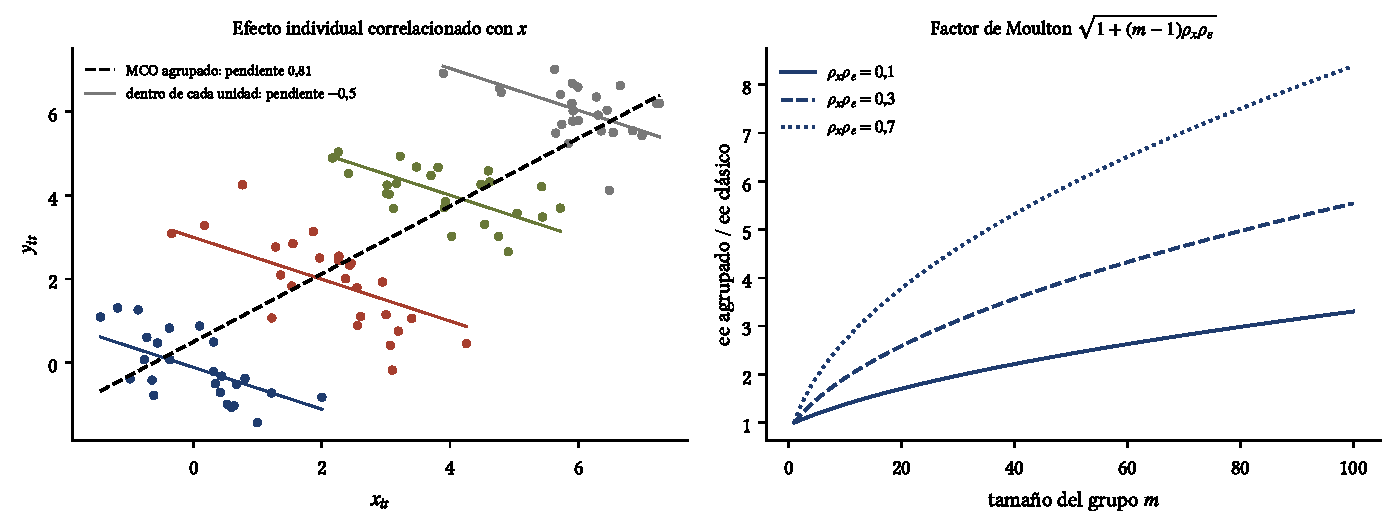
\includegraphics[width=\linewidth]{graficos/cap19_fig_teoria.pdf}
\caption{Izquierda: cuatro unidades con la misma pendiente, $-0{,}5$, pero con efectos individuales que crecen con $x$. El MCO
agrupado estima una pendiente positiva (0,81). Derecha: cuánto subestima el error estándar clásico cuando los residuos y el
regresor están correlacionados dentro de grupos de tamaño $m$.}
\label{fig:panelteoria}
\end{figure}

% ---------------------------------------------------------------------
\section{Errores estándar en paneles}
% ---------------------------------------------------------------------

Con cualquier estimador lineal $\hat{\boldsymbol\beta}=\boldsymbol\beta+(X'X)^{-1}X'\boldsymbol\varepsilon$, la varianza es
$(X'X)^{-1}X'\Omega X(X'X)^{-1}$. Lo que cambia es qué se supone sobre $\Omega=\Var(\boldsymbol\varepsilon\mid X)$:
\begin{itemize}[leftmargin=*]
  \item \textbf{Clásicos}: $\Omega=\sigma^2I$.
  \item \textbf{White}: $\Omega$ diagonal, con varianzas distintas.
  \item \textbf{Agrupados por $g$} (Liang y Zeger, 1986; Arellano, 1987): errores correlacionados de forma arbitraria dentro de
        cada grupo e independientes entre grupos, $\hat V=(X'X)^{-1}\bigl[\sum_gX_g'\hat{\boldsymbol\varepsilon}_g\hat{\boldsymbol\varepsilon}_g'X_g\bigr](X'X)^{-1}$,
        con el factor $\frac{G}{G-1}\frac{n-1}{n-K}$ en muestras finitas. Son consistentes cuando el número de grupos $G$ crece.
  \item \textbf{Dos vías} (Cameron, Gelbach y Miller, 2011; Thompson, 2011): $\hat V_{\text{empresa}}+\hat V_{\text{tiempo}}-\hat V_{\text{White}}$,
        para correlación dentro de empresas y dentro de períodos a la vez.
  \item \textbf{Driscoll y Kraay} (1998): Newey-West sobre la serie de tiempo $\mathbf h_t=\sum_i\mathbf x_{it}\hat\varepsilon_{it}$;
        robusto a correlación de corte transversal arbitraria y a autocorrelación hasta $L$ rezagos.
\end{itemize}

\begin{proposicion}[Factor de Moulton]\label{prop:moulton}
Sea un regresor $x$ y grupos de tamaño $m$ en los que, para dos observaciones distintas del mismo grupo,
\[
  \operatorname{Corr}(x_{it},x_{js})=\rho_x,\qquad \operatorname{Corr}(\varepsilon_{it},\varepsilon_{js})=\rho_\varepsilon
\]
(y cero entre grupos), con errores homocedásticos independientes de $x$. Entonces,
aproximadamente,
\[
  \frac{\Var_{\text{verdadera}}(\hat\beta)}{\Var_{\text{clásica}}(\hat\beta)}=1+(m-1)\rho_x\rho_\varepsilon .
\]
\end{proposicion}

\begin{proof}
Con $x$ centrado, $\hat\beta-\beta=\sum x_k\varepsilon_k/\sum x_k^2$. Condicionando en $x$, la varianza verdadera es
$\sum_k\sum_lx_kx_l\Cov(\varepsilon_k,\varepsilon_l)/(\sum x_k^2)^2$, y solo hay covarianzas dentro de los grupos:
\begin{align*}
  \sum_k\sum_lx_kx_l\Cov(\varepsilon_k,\varepsilon_l) &= \sigma^2\sum_kx_k^2+\rho_\varepsilon\sigma^2\sum_g\sum_{k\neq l\in g}x_kx_l .
\end{align*}
Con muchas observaciones, $\sum_g\sum_{k\neq l\in g}x_kx_l\approx(m-1)\rho_x\sum_kx_k^2$, porque cada observación tiene $m-1$
compañeras de grupo y el promedio de $x_kx_l$ entre compañeras es $\rho_x$ veces el de $x_k^2$:
\begin{align*}
  \Var_{\text{verdadera}}(\hat\beta) &\approx \frac{\sigma^2\sum_kx_k^2\,[1+(m-1)\rho_x\rho_\varepsilon]}{(\sum_kx_k^2)^2}\\
                                    &= \frac{\sigma^2}{\sum_kx_k^2}\,[1+(m-1)\rho_x\rho_\varepsilon]\\
                                    &= \Var_{\text{clásica}}(\hat\beta)\,[1+(m-1)\rho_x\rho_\varepsilon].
\end{align*}
\end{proof}

La consecuencia práctica (Moulton, 1990; Petersen, 2009) es que el sesgo de los errores clásicos solo es grande cuando
\emph{ambos}, el regresor y el residuo, están correlacionados dentro del grupo. En finanzas, el efecto empresa (una variable
persistente con un residuo persistente) pide agrupar por empresa; el efecto tiempo (un choque común que afecta a todas las
empresas en un mes y un regresor que también se mueve en común) pide agrupar por período. Con pocos grupos, por ejemplo 10
empresas, el estimador agrupado es poco fiable y conviene usar valores críticos de una $t$ con $G-1$ grados de libertad.

% ---------------------------------------------------------------------
\section{Paneles dinámicos}
% ---------------------------------------------------------------------

Si el modelo incluye la variable rezagada, $y_{it}=\rho y_{i,t-1}+\alpha_i+\varepsilon_{it}$, la exogeneidad estricta falla: $y_{i,t-1}$
depende de $\varepsilon_{i,t-1}$, que está en la media $\bar\varepsilon_i$ usada por el within. Nickell (1981) mostró que, con $N\to\infty$ y
$T$ fijo,
\[
  \operatorname{plim}\hat\rho_W-\rho\approx-\frac{1+\rho}{T-1},
\]
un sesgo negativo que solo desaparece cuando $T$ crece. Con $T=20$ y $\rho=0{,}7$, el sesgo es cercano a $-0{,}09$.

\begin{proposicion}[Instrumento de Anderson y Hsiao]\label{prop:ah}
En la ecuación en diferencias $\Delta y_{it}=\rho\,\Delta y_{i,t-1}+\Delta\varepsilon_{it}$, si los $\varepsilon_{it}$ no están
autocorrelacionados, $y_{i,t-2}$ es un instrumento válido para $\Delta y_{i,t-1}$.
\end{proposicion}

\begin{proof}
La diferencia elimina $\alpha_i$, pero $\Delta y_{i,t-1}=y_{i,t-1}-y_{i,t-2}$ está correlacionado con $\Delta\varepsilon_{it}=\varepsilon_{it}-\varepsilon_{i,t-1}$ a
través de $\varepsilon_{i,t-1}$. El nivel $y_{i,t-2}$ depende solo de $\alpha_i$ y de $\varepsilon_{i,t-2},\varepsilon_{i,t-3},\dots$:
\begin{align*}
  \E[y_{i,t-2}\,\Delta\varepsilon_{it}] &= \E[y_{i,t-2}\,\varepsilon_{it}]-\E[y_{i,t-2}\,\varepsilon_{i,t-1}]\\
                                         &= 0-0 .
\end{align*}
Y está correlacionado con $\Delta y_{i,t-1}$ (relevancia) mientras $\rho<1$, porque $\Delta y_{i,t-1}=(\rho-1)y_{i,t-2}+\alpha_i+\varepsilon_{i,t-1}$.
\end{proof}

Arellano y Bond (1991) usan como instrumentos todos los rezagos disponibles por el método generalizado de momentos, lo que
es más eficiente. Cuando $\rho$ es cercano a uno, los instrumentos en niveles son débiles y conviene el estimador de sistema de
Blundell y Bond (1998).

% ---------------------------------------------------------------------
\section{Ejercicios resueltos}
% ---------------------------------------------------------------------

\begin{ejresuelto}{La ecuación de inversión de Grunfeld}\label{ej:grunfeld}
\enunciado Estime $I_{it}=\beta_1F_{it}+\beta_2C_{it}+\alpha_i+\varepsilon_{it}$, donde $I$ es la inversión, $F$ el valor de mercado y $C$ el
stock de capital, con MCO agrupado, between, efectos fijos, efectos aleatorios y primeras diferencias. Contraste los efectos
individuales y aplique la prueba de Hausman.

\solucion
\paso{Paso 1. Estimaciones} (errores estándar clásicos entre paréntesis).
\begin{center}\small
\begin{tabular}{@{}lrr@{}}
\toprule
Estimador & Valor ($F$) & Capital ($C$) \\
\midrule
MCO agrupado & 0,1156 (0,0058) & 0,2307 (0,0255) \\
Between & 0,1346 (0,0287) & 0,0320 (0,1909) \\
Efectos fijos & 0,1101 (0,0119) & 0,3101 (0,0174) \\
Efectos aleatorios & 0,1098 (0,0105) & 0,3081 (0,0172) \\
Primeras diferencias & 0,0891 (0,0082) & 0,2787 (0,0472) \\
\bottomrule
\end{tabular}
\end{center}
Un millón más de valor de mercado se asocia con 0,11 millones más de inversión, y un millón más de capital, con 0,31. Las
estimaciones within coinciden con las de Baltagi (2001) y con \texttt{linearmodels}.

\paso{Paso 2. Efectos individuales.} La prueba $F$ de que los diez $\alpha_i$ son iguales:
\begin{align*}
  F &= \frac{(SCR_{\text{agrupado}}-SCR_W)/(N-1)}{SCR_W/(NT-N-K)}\\
    &= 49{,}18,
\end{align*}
con $(9,\,188)$ grados de libertad y valor $p$ de $10^{-44}$. Los efectos fijos estimados van de $-235{,}6$ a $101{,}9$.

\paso{Paso 3. Efectos aleatorios y Hausman.} Con $\hat\sigma_u=84{,}20$ y $\hat\sigma_\varepsilon=52{,}77$:
\begin{align*}
  \theta &= 1-\frac{52{,}77}{\sqrt{52{,}77^2+20\times84{,}20^2}}\\
         &= 1-\frac{52{,}77}{\sqrt{2\,784{,}7+141\,793}}\\
         &= 1-\frac{52{,}77}{380{,}23}\\
         &= 0{,}861 .
\end{align*}
Con $\theta$ tan cerca de uno, efectos aleatorios casi coincide con efectos fijos. El estadístico de Hausman es $H=2{,}33$ con valor
$p=0{,}31$: no se rechaza que los efectos sean aleatorios, y efectos aleatorios es preferible por eficiencia
(Figura~\ref{fig:grunfeld}).

\codigoweb{cap19_ej01}
\salidaR{cap19_ej01_R.txt}
\lectura{cap19_ej01}

\RvsPy La transformación within usa \texttt{ave(z, g)} en R, que devuelve la media del grupo repetida en cada observación, y una
función equivalente con \texttt{np.bincount} en Python. Los paquetes especializados son \texttt{plm} en R y \texttt{linearmodels}
en Python (\texttt{PanelOLS}, \texttt{RandomEffects}); con este último comprobamos los coeficientes de efectos fijos y aleatorios,
incluido $\theta=0{,}8612$. Las primeras diferencias requieren ordenar por empresa y año antes de restar.

\begin{figure}[ht]
\centering
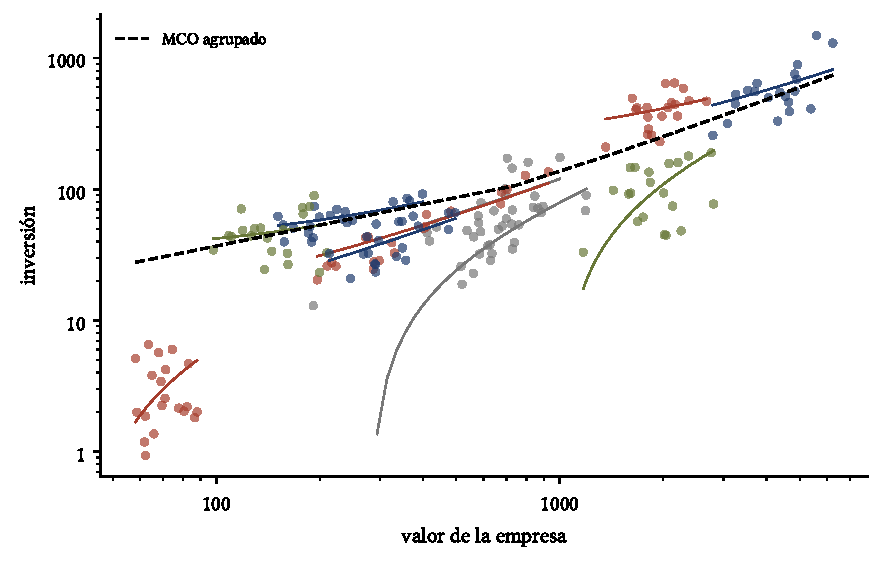
\includegraphics[width=0.78\linewidth]{graficos/cap19_ej01_grunfeld.pdf}
\caption{Inversión frente a valor de mercado de las 10 empresas (escala logarítmica), con las rectas de efectos fijos de cada empresa
(evaluadas en su capital medio y dibujadas donde la inversión ajustada es positiva) y la del MCO agrupado (discontinua).}
\label{fig:grunfeld}
\end{figure}

\begin{conclusion}
Las empresas difieren mucho en su nivel de inversión, pero esas diferencias no están correlacionadas con el valor y el capital lo
suficiente como para sesgar las pendientes: los cuatro estimadores consistentes con efectos individuales dan resultados similares,
y el MCO agrupado subestima el efecto del capital.
\end{conclusion}
\end{ejresuelto}

\begin{ejresuelto}{Errores estándar con pocas empresas}\label{ej:errores}
\enunciado Para el modelo de efectos fijos de Grunfeld, calcule los errores estándar clásicos, de White, agrupados por empresa, por
año, en dos vías y de Driscoll-Kraay. Estime también el modelo con efectos fijos de empresa y de año.

\solucion
\paso{Paso 1. La estructura de los residuos.} La autocorrelación media de orden 1 de los residuos de cada empresa es 0,632, y la
correlación media entre los residuos de dos empresas en el mismo año, 0,155: hay un efecto empresa fuerte y un efecto tiempo moderado.

\paso{Paso 2. Errores estándar.}
\begin{center}\small
\begin{tabular}{@{}lrrrr@{}}
\toprule
Método & ee(valor) & ee(capital) & $t$(valor) & $t$(capital) \\
\midrule
Clásicos & 0,0119 & 0,0174 & 9,29 & 17,87 \\
White & 0,0194 & 0,0428 & 5,68 & 7,25 \\
Agrupados por empresa & 0,0156 & 0,0540 & 7,08 & 5,74 \\
Agrupados por año & 0,0173 & 0,0323 & 6,36 & 9,61 \\
Dos vías & 0,0129 & 0,0461 & 8,53 & 6,72 \\
Driscoll-Kraay ($L=2$) & 0,0177 & 0,0348 & 6,23 & 8,90 \\
\bottomrule
\end{tabular}
\end{center}
El error estándar del capital se triplica al agrupar por empresa, coherente con la persistencia de los residuos. Aun así, todos los
coeficientes siguen siendo significativos, incluso con el valor crítico de la $t_9$ ($2{,}262$) que corresponde a 10 grupos.

\paso{Paso 3. Efectos de año.} Con efectos fijos de empresa y de año, $\hat\beta_F=0{,}1177$ y $\hat\beta_C=0{,}3579$. Los efectos de año van de
$+47{,}3$ (1935) a $-46{,}2$ (1954) respecto de la media, con un patrón descendente que recoge cambios comunes en la inversión que
no explican el valor y el capital.

\codigoweb{cap19_ej02}
\salidaR{cap19_ej02_R.txt}
\lectura{cap19_ej02}

\RvsPy Todas las matrices de varianza usan el mismo ``pan'' $(X'X)^{-1}$ y cambian el ``relleno''. En R, \texttt{sandwich::vcovCL}
y \texttt{sandwich::vcovPL} implementan los agrupados y Driscoll-Kraay; en Python, \texttt{linearmodels} con
\texttt{cov\_type="clustered"} o \texttt{"kernel"}. El factor de muestra finita varía entre programas (aquí, el de Stata), por lo
que conviene informar cuál se usa.

\begin{conclusion}
Los errores clásicos subestiman la incertidumbre hasta en un factor de tres. Con solo 10 empresas, ningún método agrupado es del
todo fiable: el panel de Grunfeld es largo y angosto, y los métodos de series de tiempo como Driscoll-Kraay son una alternativa
razonable.
\end{conclusion}
\end{ejresuelto}

\begin{ejresuelto}{El sesgo de Nickell}\label{ej:nickell}
\enunciado Estime $\ln I_{it}=\rho\ln I_{i,t-1}+\beta\ln F_{it}+\alpha_i+\varepsilon_{it}$ con MCO agrupado, efectos fijos y Anderson-Hsiao. Luego
simule 1\,000 paneles con $N=10$, $T=20$ y $\rho=0{,}7$ para medir el sesgo de efectos fijos.

\solucion
\paso{Paso 1. Datos reales.}
\begin{center}\small
\begin{tabular}{@{}lrrr@{}}
\toprule
Estimador & $\hat\rho$ & $\hat\beta$ & $n$ \\
\midrule
MCO agrupado & 0,914 (0,024) & 0,102 (0,028) & 190 \\
Efectos fijos & 0,700 (0,045) & 0,442 (0,076) & 190 \\
Anderson-Hsiao & 0,498 (0,288) & 0,691 (0,113) & 180 \\
\bottomrule
\end{tabular}
\end{center}
El MCO agrupado sobrestima la persistencia, porque atribuye a $\rho$ las diferencias permanentes entre empresas. Efectos fijos la
reduce, pero tiene sesgo de Nickell hacia abajo. Anderson-Hsiao es consistente, pero muy impreciso: su instrumento tiene una
correlación de apenas $-0{,}066$ con el regresor endógeno, un instrumento débil.

\paso{Paso 2. Simulación.} Con 19 observaciones efectivas por empresa, la fórmula de Nickell da
\begin{align*}
  -\frac{1+0{,}7}{19-1} &= -\frac{1{,}7}{18}\\
                       &= -0{,}094 .
\end{align*}
En la simulación, efectos fijos promedia $0{,}591$: un sesgo de $-0{,}109$, algo mayor que la aproximación (que es para $N$ grande), y
1,7 veces su desviación estándar (0,062). Anderson-Hsiao tiene una mediana de $0{,}711$, casi sin sesgo, pero con un rango
intercuartílico de 0,243, casi cuatro veces la desviación estándar de efectos fijos (Figura~\ref{fig:nickell}).

\codigoweb{cap19_ej03}
\salidaR{cap19_ej03_R.txt}
\lectura{cap19_ej03}

\RvsPy Los rezagos dentro de cada empresa se construyen con una tabla de búsqueda por (empresa, año): \texttt{match} con claves de
texto en R y un diccionario en Python, lo que evita mezclar el último año de una empresa con el primero de la siguiente. La
simulación usa el generador de Park y Miller con el método de Box y Muller, como en los Capítulos~\ref{cap:eventos}
y~\ref{cap:copulas}, y descarta 50 períodos iniciales.

\begin{figure}[ht]
\centering
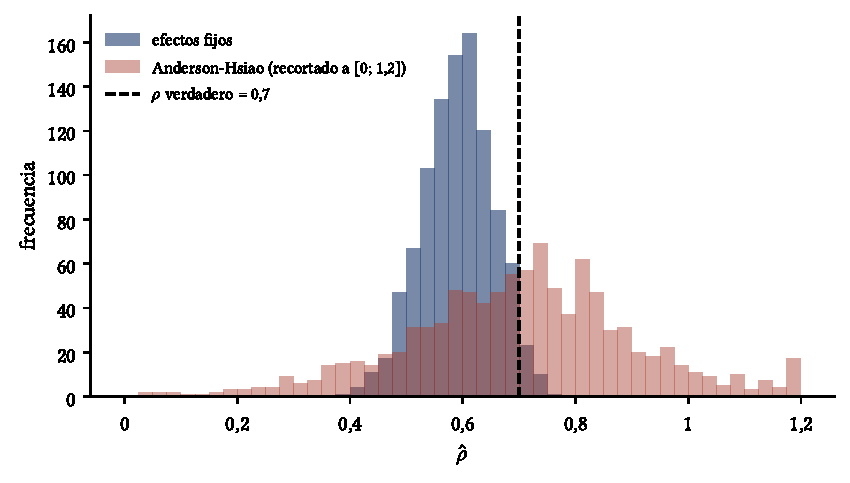
\includegraphics[width=0.78\linewidth]{graficos/cap19_ej03_nickell.pdf}
\caption{Distribución de $\hat\rho$ en 1\,000 paneles simulados con $N=10$, $T=20$ y $\rho=0{,}7$: efectos fijos (sesgado hacia abajo) y
Anderson-Hsiao (centrado, pero muy disperso).}
\label{fig:nickell}
\end{figure}

\begin{conclusion}
En paneles dinámicos cortos, efectos fijos subestima la persistencia y los estimadores de variables instrumentales la corrigen a
costa de mucha varianza. Con $T=20$ el sesgo de Nickell es comparable al error estándar, y no puede ignorarse.
\end{conclusion}
\end{ejresuelto}

\begin{ejresuelto}{¿Qué errores estándar? Un panel de carteras}\label{ej:petersen}
\enunciado Con el panel de 30 carteras y 807 meses, estime por MCO agrupado la regresión del exceso de rendimiento del mes $t$ sobre el
rendimiento acumulado de $t-12$ a $t-2$ (la señal de momentum). Compare los errores estándar de la pendiente con todos los métodos y
con Fama-MacBeth.

\solucion
\paso{Paso 1. Estructura de los datos.} Dentro de un mismo mes, los residuos de dos carteras tienen una correlación media de 0,708, y
la señal, de 0,700: un efecto tiempo enorme, porque todas las carteras se mueven con el mercado. En cambio, los residuos de una cartera
casi no están autocorrelacionados (0,101), aunque la señal sí lo está (0,921): el efecto cartera es pequeño.

\paso{Paso 2. Errores estándar.} La pendiente agrupada es $-0{,}00027$.
\begin{center}\small
\begin{tabular}{@{}lrrr@{}}
\toprule
Método & ee & $t$ & Cociente con el clásico \\
\midrule
Clásicos & 0,00180 & $-0{,}15$ & 1,00 \\
White & 0,00272 & $-0{,}10$ & 1,51 \\
Agrupados por cartera & 0,00117 & $-0{,}23$ & 0,65 \\
Agrupados por mes & 0,01038 & $-0{,}03$ & 5,75 \\
Dos vías & 0,01008 & $-0{,}03$ & 5,59 \\
Driscoll-Kraay ($L=12$) & 0,00921 & $-0{,}03$ & 5,10 \\
\midrule
Fama-MacBeth & 0,00430 & 6,18 & 2,38 \\
Fama-MacBeth con Newey-West & 0,00410 & 6,48 & 2,27 \\
\bottomrule
\end{tabular}
\end{center}
El error clásico subestima en un factor de casi 6 porque ignora el efecto tiempo. La Proposición~\ref{prop:moulton} lo anticipa:
\begin{align*}
  \sqrt{1+(30-1)\times0{,}700\times0{,}708} &= \sqrt{1+14{,}37}\\
                                             &= 3{,}92,
\end{align*}
que multiplicado por el factor de heterocedasticidad (1,51) da 5,9, cerca del 5,75 observado. Agrupar por cartera no sirve aquí:
el efecto cartera es débil y ese método ignora la correlación entre carteras.

\paso{Paso 3. Fama-MacBeth.} La pendiente media de las 807 regresiones de corte transversal es $0{,}02656$ con $t=6{,}18$: un resultado
opuesto al agrupado. No es un problema de errores estándar sino de \emph{qué se estima}, que es el tema del ejercicio siguiente. Las
pendientes mensuales casi no están autocorrelacionadas (0,099), por lo que la corrección de Newey-West apenas cambia el error
(Figura~\ref{fig:errores19}).

\codigoweb{cap19_ej04}
\salidaR{cap19_ej04_R.txt}
\lectura{cap19_ej04}

\RvsPy El panel se arma en formato largo, con una fila por cartera y mes, desde las matrices $T\times N$: \texttt{as.vector(t(R))} en R
recorre por filas como \texttt{R.ravel()} en Python. Las 807 pendientes de Fama-MacBeth salen de \texttt{lm} en R y de
\texttt{np.polyfit} en Python.

\begin{figure}[ht]
\centering
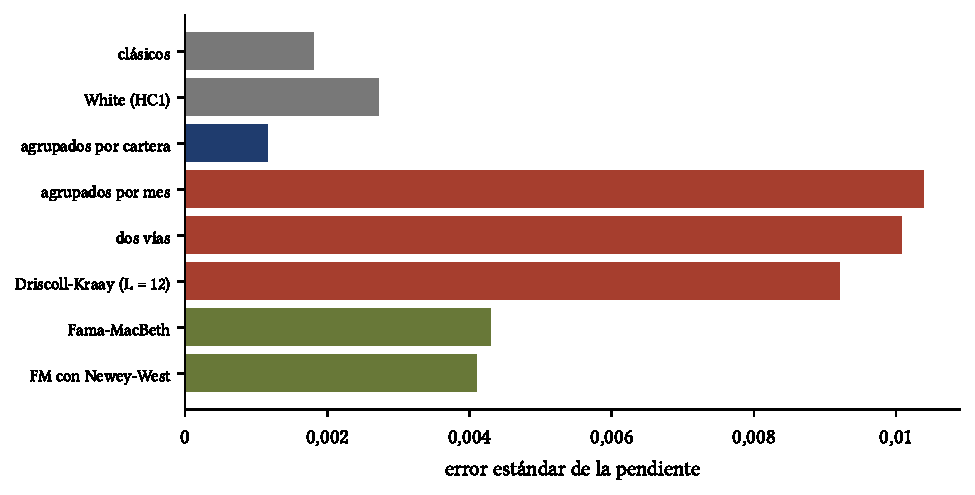
\includegraphics[width=0.85\linewidth]{graficos/cap19_ej04_errores.pdf}
\caption{Error estándar de la pendiente con cada método. Los que permiten correlación dentro del mes (rojo) son entre 5 y 6 veces el
clásico.}
\label{fig:errores19}
\end{figure}

\begin{conclusion}
En paneles de rendimientos, el efecto tiempo domina y los errores deben agruparse por período (o usar Driscoll-Kraay o
Fama-MacBeth). En paneles de finanzas corporativas, con variables persistentes como el apalancamiento, suele dominar el efecto empresa.
La regla de Petersen es calcular ambos y, si difieren, usar los de dos vías.
\end{conclusion}
\end{ejresuelto}

\begin{ejresuelto}{Momentum de series de tiempo y de corte transversal}\label{ej:descomposicion}
\enunciado Reestime la regresión del ejercicio anterior con efectos fijos de cartera, de mes y de ambos, con errores agrupados en dos
vías. Explique con la Proposición~\ref{prop:mezclapanel} por qué el estimador agrupado es casi cero.

\solucion
\paso{Paso 1. Especificaciones.}
\begin{center}\small
\begin{tabular}{@{}lrrrr@{}}
\toprule
Efectos fijos & Pendiente & ee (dos vías) & $t$ & Varianza de $x$ usada \\
\midrule
Ninguno & $-0{,}00027$ & 0,01008 & $-0{,}03$ & 1,000 \\
Cartera & $-0{,}00251$ & 0,01021 & $-0{,}25$ & 0,976 \\
Mes & 0,01634 & 0,00673 & 2,43 & 0,327 \\
Cartera y mes & 0,01045 & 0,00667 & 1,57 & 0,303 \\
\bottomrule
\end{tabular}
\end{center}
Con efectos de mes, solo se compara cada cartera con las demás \emph{en el mismo mes}: las de mejor rendimiento pasado rinden más
después, el momentum de corte transversal de Jegadeesh y Titman (1993). Diez puntos más de rendimiento pasado anticipan 0,163 puntos
más de rendimiento mensual.

\paso{Paso 2. La descomposición.} El 67,3\,\% de la varianza de la señal es \emph{entre meses} (todas las carteras subieron o bajaron
juntas), y en esa dimensión la relación es negativa: la regresión del rendimiento medio del mes sobre la señal media da $-0{,}00834$. Por
la Proposición~\ref{prop:mezclapanel}, con los meses como grupos:
\begin{align*}
  \hat\beta_{\text{agrupado}} &= 0{,}3270\times0{,}01634+0{,}6730\times(-0{,}00834)\\
                              &= 0{,}00534-0{,}00561\\
                              &= -0{,}00027 .
\end{align*}
Los dos efectos se cancelan. El MCO agrupado, que parecía decir que el momentum no existe, promedia una relación de corte transversal
positiva con una de series de tiempo del mercado negativa (Figura~\ref{fig:descomposicion}).

\paso{Paso 3. Relación con Fama-MacBeth.} Efectos fijos de mes y Fama-MacBeth usan la misma variación de corte transversal, pero
ponderan los meses de forma distinta: Fama-MacBeth da igual peso a cada mes, y la regresión con efectos de mes pondera cada mes por la
dispersión de la señal en ese mes. Por eso sus pendientes difieren (0,0266 y 0,0163) aunque ambas son positivas.

\codigoweb{cap19_ej05}
\salidaR{cap19_ej05_R.txt}
\lectura{cap19_ej05}

\RvsPy Con un panel balanceado, los efectos fijos en dos vías se eliminan restando las medias de cartera y de mes y sumando la media
total; con un panel desbalanceado esa fórmula no es exacta y hay que iterar o usar ficticias. Los grados de libertad que restan los
efectos fijos ($N-1$ y $T-1$) se descuentan en el factor de muestra finita de los errores agrupados.

\begin{figure}[ht]
\centering
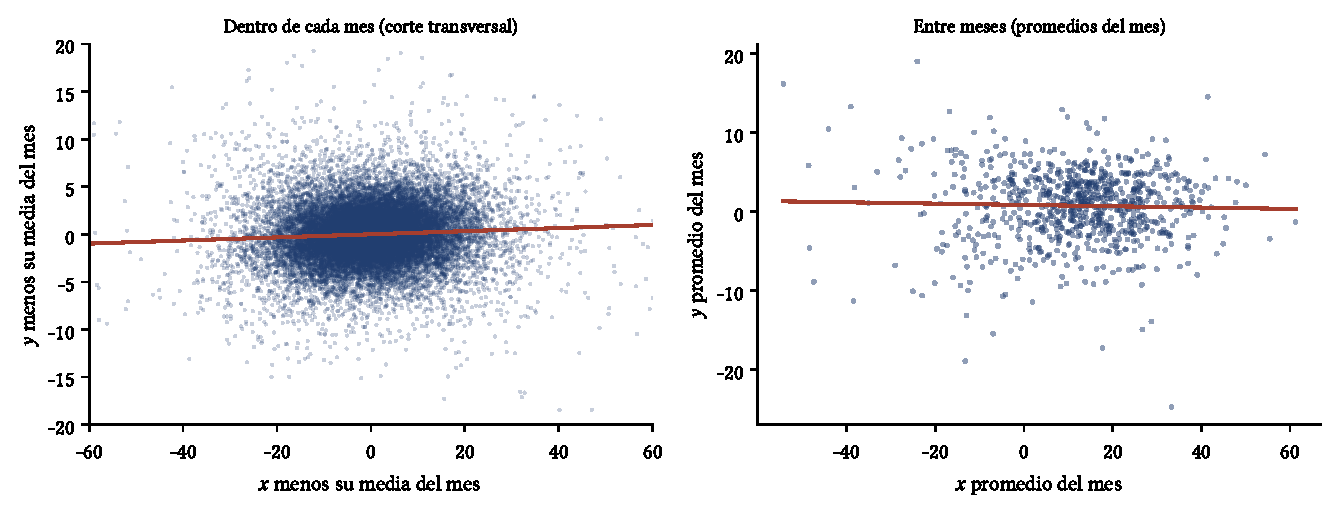
\includegraphics[width=\linewidth]{graficos/cap19_ej05_descomposicion.pdf}
\caption{Izquierda: relación de corte transversal (desviaciones respecto de la media del mes), con pendiente positiva. Derecha: relación
entre meses (promedios de las 30 carteras), con pendiente negativa.}
\label{fig:descomposicion}
\end{figure}

\begin{conclusion}
Los efectos fijos no son solo un control: deciden qué variación identifica el coeficiente. En valoración de activos, la pregunta suele
ser de corte transversal, y la especificación correcta incluye efectos de período o usa Fama-MacBeth.
\end{conclusion}
\end{ejresuelto}

% ---------------------------------------------------------------------
\section{Ejercicios propuestos}
% ---------------------------------------------------------------------

\begin{enumerate}[label=\textbf{\thechapter.\arabic*},leftmargin=*,itemsep=6pt]
  \item Con $\sigma_\varepsilon=2$, $\sigma_u=3$ y $T=8$, calcule $\theta$ del estimador de efectos aleatorios. \textit{Respuesta:
  $1-2/\sqrt{4+72}=0{,}7706$.}

  \item En un panel de 50 empresas y 20 años, la correlación de los residuos dentro de cada empresa es 0,4 y la del regresor, 0,8.
  ¿Cuánto subestiman los errores clásicos? \textit{Respuesta: un factor de $\sqrt{1+19\times0{,}32}=2{,}66$.}

  \item Con $T=10$ y $\rho=0{,}5$, calcule el sesgo aproximado de Nickell. \textit{Respuesta: $-1{,}5/9=-0{,}167$.}

  \item Demuestre que con $T=2$ el estimador de efectos fijos y el de primeras diferencias son idénticos.

  \item Demuestre la versión matricial de la Proposición~\ref{prop:mezclapanel}:
  $\hat{\boldsymbol\beta}_{\text{agrupado}}=(S_W+S_B)^{-1}(S_W\hat{\boldsymbol\beta}_W+S_B\hat{\boldsymbol\beta}_B)$, con $S_W$ y $S_B$ matrices.

  \item \emph{(Simulación.)} Simule paneles de 500 empresas y 10 años con efecto empresa ($\rho_x=\rho_\varepsilon=0{,}5$) y estime la frecuencia de
  rechazo al 5\,\% de una hipótesis verdadera con errores clásicos, de White y agrupados por empresa (Petersen, 2009).

  \item \emph{(Con datos de la SMV.)} Con los estados financieros de las empresas listadas en la BVL, estime la relación entre
  apalancamiento y rentabilidad con efectos fijos de empresa y de año. ¿Qué dimensión de agrupamiento importa más?

  \item \emph{(Con datos.)} Repita el Ejercicio~\ref{ej:descomposicion} usando solo las 12 industrias. ¿Hay momentum de industrias
  (Moskowitz y Grinblatt, 1999)?
\end{enumerate}

% ---------------------------------------------------------------------
\section{Resumen de fórmulas}
% ---------------------------------------------------------------------

\begin{table}[H]
\centering\small
\begin{tabular}{@{}ll@{}}
\toprule
Concepto & Fórmula \\
\midrule
Within & $\ddot y_{it}=y_{it}-\bar y_i$;\quad $\hat{\boldsymbol\beta}_W=(\sum\ddot{\mathbf x}\ddot{\mathbf x}')^{-1}\sum\ddot{\mathbf x}\ddot y$;\quad gl $=NT-N-K$ \\
Efectos aleatorios & $y_{it}-\theta\bar y_i$;\quad $\theta=1-\sigma_\varepsilon/\sqrt{\sigma_\varepsilon^2+T\sigma_u^2}$ \\
Hausman & $(\hat{\boldsymbol\beta}_{FE}-\hat{\boldsymbol\beta}_{RE})'[\hat V_{FE}-\hat V_{RE}]^{-1}(\cdot)\sim\chi^2_K$ \\
Agrupado = mezcla & $\hat\beta=\frac{S_W}{S_W+S_B}\hat\beta_W+\frac{S_B}{S_W+S_B}\hat\beta_B$ \\
Errores agrupados & $(X'X)^{-1}\sum_gX_g'\hat{\boldsymbol\varepsilon}_g\hat{\boldsymbol\varepsilon}_g'X_g(X'X)^{-1}\cdot\frac{G}{G-1}\frac{n-1}{n-K}$ \\
Dos vías & $\hat V_{\text{empresa}}+\hat V_{\text{tiempo}}-\hat V_{\text{White}}$ \\
Factor de Moulton & $1+(m-1)\rho_x\rho_\varepsilon$ \\
Sesgo de Nickell & $\approx-(1+\rho)/(T-1)$ \\
Anderson-Hsiao & $\Delta y_{it}=\rho\Delta y_{i,t-1}+\Delta\varepsilon_{it}$, instrumento $y_{i,t-2}$ \\
\bottomrule
\end{tabular}
\caption{Fórmulas principales del Capítulo 19.}
\end{table}

\section*{Referencias}
\begin{itemize}[leftmargin=*]
  \item Anderson, T. W. y Hsiao, C. (1981). Estimation of dynamic models with error components. \emph{Journal of the American
        Statistical Association}, 76(375), 598--606.
  \item Arellano, M. (1987). Computing robust standard errors for within-groups estimators. \emph{Oxford Bulletin of Economics and
        Statistics}, 49(4), 431--434.
  \item Arellano, M. y Bond, S. (1991). Some tests of specification for panel data: Monte Carlo evidence and an application to
        employment equations. \emph{Review of Economic Studies}, 58(2), 277--297.
  \item Baltagi, B. H. (2001). \emph{Econometric Analysis of Panel Data}, 3.ª ed. Wiley.
  \item Blundell, R. y Bond, S. (1998). Initial conditions and moment restrictions in dynamic panel data models. \emph{Journal of
        Econometrics}, 87(1), 115--143.
  \item Cameron, A. C., Gelbach, J. B. y Miller, D. L. (2011). Robust inference with multiway clustering. \emph{Journal of
        Business \& Economic Statistics}, 29(2), 238--249.
  \item Driscoll, J. C. y Kraay, A. C. (1998). Consistent covariance matrix estimation with spatially dependent panel data.
        \emph{Review of Economics and Statistics}, 80(4), 549--560.
  \item Grunfeld, Y. (1958). \emph{The Determinants of Corporate Investment}. Tesis doctoral, Universidad de Chicago.
  \item Hausman, J. A. (1978). Specification tests in econometrics. \emph{Econometrica}, 46(6), 1251--1271.
  \item Jegadeesh, N. y Titman, S. (1993). Returns to buying winners and selling losers: Implications for stock market
        efficiency. \emph{Journal of Finance}, 48(1), 65--91.
  \item Kleiber, C. y Zeileis, A. (2010). The Grunfeld data at 50. \emph{German Economic Review}, 11(4), 404--417.
  \item Liang, K.-Y. y Zeger, S. L. (1986). Longitudinal data analysis using generalized linear models. \emph{Biometrika}, 73(1),
        13--22.
  \item Moskowitz, T. J. y Grinblatt, M. (1999). Do industries explain momentum? \emph{Journal of Finance}, 54(4), 1249--1290.
  \item Moulton, B. R. (1990). An illustration of a pitfall in estimating the effects of aggregate variables on micro units.
        \emph{Review of Economics and Statistics}, 72(2), 334--338.
  \item Nickell, S. (1981). Biases in dynamic models with fixed effects. \emph{Econometrica}, 49(6), 1417--1426.
  \item Petersen, M. A. (2009). Estimating standard errors in finance panel data sets: Comparing approaches. \emph{Review of
        Financial Studies}, 22(1), 435--480.
  \item Swamy, P. A. V. B. y Arora, S. S. (1972). The exact finite sample properties of the estimators of coefficients in the error
        components regression models. \emph{Econometrica}, 40(2), 261--275.
  \item Thompson, S. B. (2011). Simple formulas for standard errors that cluster by both firm and time. \emph{Journal of Financial
        Economics}, 99(1), 1--10.
\end{itemize}

% =====================================================================
%  Capítulo 20. Aprendizaje automático en finanzas
% =====================================================================
\chapter[Aprendizaje automático]{Aprendizaje automático en finanzas: contracción, validación y árboles}\label{cap:aprendizaje}

\section*{Objetivos de aprendizaje}
Al terminar este capítulo, el lector podrá:
\begin{enumerate}[label=\arabic*.,leftmargin=*]
  \item Explicar el dilema entre sesgo y varianza y por qué un modelo que ajusta mejor dentro de la muestra puede
        pronosticar peor fuera de ella.
  \item Estimar ridge, lasso y red elástica, derivar sus soluciones y elegir la penalización con validación que
        respete el orden del tiempo.
  \item Evaluar pronósticos de rendimientos fuera de muestra con el $R^2$ fuera de muestra, la prueba de Clark y
        West y su valor económico para un inversionista.
  \item Clasificar eventos con regresión logística y medir la calidad de la clasificación con la curva ROC, y
        reconocer el sobreajuste de los árboles de regresión.
\end{enumerate}

\section*{Motivación}
El aprendizaje automático promete extraer señales de muchas variables con métodos flexibles. En finanzas esa promesa
choca con un hecho del Capítulo~\ref{cap:eficiencia}: los rendimientos son casi impredecibles, de modo que la señal es
diminuta frente al ruido. En ese ambiente, la flexibilidad es peligrosa: un modelo con muchos parámetros ajusta el
ruido de la muestra y pronostica peor que la media histórica. Goyal y Welch (2008) mostraron que casi ningún predictor
clásico de la prima de mercado supera a la media fuera de muestra. Las técnicas de este capítulo, la contracción, la
validación temporal y la combinación de pronósticos, son las herramientas para no engañarse. Gu, Kelly y Xiu (2020)
encontraron ganancias reales con redes y árboles en el corte transversal de miles de acciones; aquí trabajamos con un
problema más pequeño que permite ver cada paso.

\paragraph{Datos del capítulo.} Diez predictores mensuales del exceso de rendimiento del mercado de EE.\,UU. del mes
siguiente, de septiembre de 1927 a noviembre de 2018 ($n=1\,095$), construidos con la base de Robert Shiller y la de
Kenneth French: razón dividendo/precio ($dp$), beneficio/precio ($ep$), dividendo/beneficio ($de$), CAPE, rendimiento del
bono a 10 años ($lty$), tasa de las letras ($tbl$), pendiente ($tms=lty-tbl$), inflación de 12 meses rezagada, momentum de 12
meses y volatilidad de 12 meses del mercado. Para la clasificación, la curva de rendimientos de McCulloch y Kwon del
Capítulo~\ref{cap:tasas} y las recesiones del NBER.

% ---------------------------------------------------------------------
\section{Sesgo, varianza y validación}
% ---------------------------------------------------------------------

Sea $y=f(\mathbf x)+\varepsilon$ con $\E[\varepsilon\mid\mathbf x]=0$ y $\Var(\varepsilon)=\sigma^2$, y sea $\hat f$ un estimador obtenido con una
muestra de entrenamiento independiente de un punto nuevo $(\mathbf x_0,y_0)$.

\begin{proposicion}[Descomposición sesgo-varianza]\label{prop:sesgovarianza}
\[
  \E\bigl[(y_0-\hat f(\mathbf x_0))^2\bigr]=\sigma^2+\bigl[\E\hat f(\mathbf x_0)-f(\mathbf x_0)\bigr]^2+\Var\bigl(\hat f(\mathbf x_0)\bigr).
\]
\end{proposicion}

\begin{proof}
Escribimos $y_0-\hat f=\varepsilon_0+(f-\E\hat f)+(\E\hat f-\hat f)$, donde todo se evalúa en $\mathbf x_0$. El primer término es
independiente de los otros dos (viene del punto nuevo) y el tercero tiene media cero:
\begin{align*}
  \E[(y_0-\hat f)^2] &= \E[\varepsilon_0^2]+(f-\E\hat f)^2+\E[(\E\hat f-\hat f)^2]+2(f-\E\hat f)\,\E[\E\hat f-\hat f]+2\E[\varepsilon_0]\,\E[\cdots]\\
                     &= \sigma^2+(f-\E\hat f)^2+\Var(\hat f)+0+0 .
\end{align*}
\end{proof}

El primer término no se puede reducir. Un modelo más flexible reduce el sesgo y aumenta la varianza. Cuando $\sigma^2$ es
enorme frente a la parte predecible, como en los rendimientos, la varianza de un modelo flexible domina y el error fuera de
muestra crece. La Figura~\ref{fig:teoria20} (derecha) lo muestra con polinomios ajustados a 40 puntos: el error de
entrenamiento cae siempre, pero el de datos nuevos es mínimo con grado 3 (0,167, cerca del ruido, 0,16) y se dispara a 4,75 con
grado 12.

\paragraph{Validación temporal.} La validación cruzada habitual reparte las observaciones al azar en $K$ grupos. Con series de
tiempo eso usa el futuro para predecir el pasado y aprovecha la persistencia de los predictores. Lo correcto es validar
siempre \emph{hacia adelante}: estimar con los datos hasta una fecha y medir el error en los meses siguientes. En este
capítulo, el parámetro de penalización se elige con los últimos 120 meses de cada muestra de entrenamiento, y el modelo
elegido se evalúa en meses que nunca intervinieron en la estimación.

% ---------------------------------------------------------------------
\section{Contracción: ridge, lasso y red elástica}
% ---------------------------------------------------------------------

Con predictores estandarizados (media 0 y varianza 1) y $y$ centrada, los estimadores penalizados resuelven
\[
  \min_{\boldsymbol\beta}\ \frac{1}{2n}\lVert\mathbf y-X\boldsymbol\beta\rVert^2+\lambda\Bigl[\alpha\lVert\boldsymbol\beta\rVert_1+\frac{1-\alpha}{2}\lVert\boldsymbol\beta\rVert_2^2\Bigr],
\]
con $\alpha=0$ (ridge; Hoerl y Kennard, 1970), $\alpha=1$ (lasso; Tibshirani, 1996) o intermedio (red elástica; Zou y Hastie, 2005).
La penalización empuja los coeficientes hacia cero: introduce sesgo a cambio de menos varianza.

\begin{proposicion}[Ridge y lasso con regresores ortonormales]\label{prop:contraccion}
Si $X'X/n=I$ y $\hat\beta_j=\mathbf x_j'\mathbf y/n$ es el estimador de MCO, entonces
\[
  \hat\beta_j^{\text{ridge}}=\frac{\hat\beta_j}{1+\lambda},\qquad
  \hat\beta_j^{\text{lasso}}=S(\hat\beta_j,\lambda)=\operatorname{signo}(\hat\beta_j)\max(|\hat\beta_j|-\lambda,0).
\]
\end{proposicion}

\begin{proof}
Con $X'X/n=I$, el objetivo se separa en un término por coeficiente. Desarrollando el cuadrado,
$\frac1{2n}\lVert\mathbf y-X\boldsymbol\beta\rVert^2=\frac1{2n}\lVert\mathbf y\rVert^2-\sum_j\beta_j\hat\beta_j+\frac12\sum_j\beta_j^2$, de modo que para cada $j$ se minimiza
$\frac12\beta_j^2-\beta_j\hat\beta_j+\text{penalización}$.

Ridge ($\alpha=0$):
\begin{align*}
  \frac{d}{d\beta_j}\Bigl[\tfrac12\beta_j^2-\beta_j\hat\beta_j+\tfrac\lambda2\beta_j^2\Bigr] &= \beta_j-\hat\beta_j+\lambda\beta_j=0\\
  \beta_j(1+\lambda) &= \hat\beta_j\\
  \beta_j &= \hat\beta_j/(1+\lambda).
\end{align*}
Lasso ($\alpha=1$): la función $\frac12\beta_j^2-\beta_j\hat\beta_j+\lambda|\beta_j|$ es convexa y su subgradiente es $\beta_j-\hat\beta_j+\lambda s$, con
$s=\operatorname{signo}(\beta_j)$ si $\beta_j\neq0$ y $s\in[-1,1]$ si $\beta_j=0$. Si $\beta_j>0$:
\begin{align*}
  \beta_j-\hat\beta_j+\lambda &= 0\\
  \beta_j &= \hat\beta_j-\lambda,
\end{align*}
lo que es positivo solo si $\hat\beta_j>\lambda$. Simétricamente, $\beta_j=\hat\beta_j+\lambda$ si $\hat\beta_j<-\lambda$. Si
$|\hat\beta_j|\le\lambda$, $\beta_j=0$ cumple la condición con $s=\hat\beta_j/\lambda\in[-1,1]$. Las tres situaciones son
$S(\hat\beta_j,\lambda)$.
\end{proof}

Ridge reduce todos los coeficientes en la misma proporción; lasso resta una cantidad fija y pone en cero los pequeños, de modo
que también \emph{selecciona} variables (Figura~\ref{fig:teoria20}, izquierda). Sin ortonormalidad no hay fórmula cerrada para el
lasso, pero el mismo argumento aplicado a una coordenada a la vez, con las demás fijas, da el algoritmo de \emph{descenso por
coordenadas} (Friedman, Hastie y Tibshirani, 2010): con el residuo parcial $\mathbf r_{-j}$,
\[
  \beta_j\leftarrow\frac{S\bigl(\mathbf x_j'\mathbf r_{-j}/n,\ \lambda\alpha\bigr)}{1+\lambda(1-\alpha)},
\]
que se repite sobre todos los $j$ hasta que nada cambie. Es el que programamos en R y en Python.

\begin{figure}[ht]
\centering
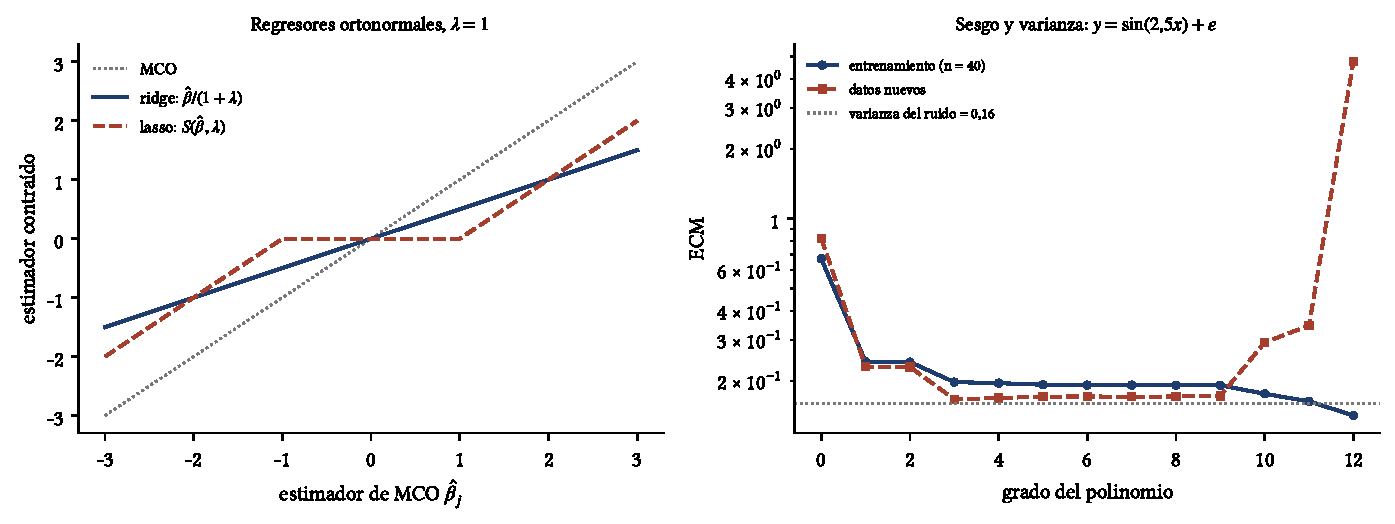
\includegraphics[width=\linewidth]{graficos/cap20_fig_teoria.pdf}
\caption{Izquierda: ridge contrae en proporción y lasso aplica un umbral suave que anula los coeficientes pequeños. Derecha: error de
entrenamiento y de datos nuevos de polinomios de grado creciente ajustados a 40 observaciones (escala logarítmica).}
\label{fig:teoria20}
\end{figure}

% ---------------------------------------------------------------------
\section{Evaluar pronósticos de rendimientos}
% ---------------------------------------------------------------------

El pronóstico de referencia es la media histórica $\bar y_t$, que no usa predictores. Campbell y Thompson (2008) definen
\[
  R^2_{OS}=1-\frac{\sum_t(y_{t+1}-\hat y_{t+1})^2}{\sum_t(y_{t+1}-\bar y_t)^2},
\]
que es positivo solo si el modelo tiene menor error cuadrático que la media. Para contrastar $H_0$: $R^2_{OS}\le0$ con modelos
anidados se usa el estadístico de Clark y West (2007), que corrige el ruido que introduce estimar parámetros que en la
población son cero: la $t$ de la media de $f_{t+1}=(y-\bar y)^2-[(y-\hat y)^2-(\bar y-\hat y)^2]$, con valor crítico unilateral.

Un $R^2$ pequeño puede valer mucho.

\begin{proposicion}[Valor de un $R^2$ pequeño]\label{prop:ct}
Sea $r_{t+1}=\mu+x_t+\varepsilon_{t+1}$, con $\E[x_t]=0$, $\Var(x_t)=R^2\sigma^2$ y $\Var(\varepsilon)=(1-R^2)\sigma^2$, y sea $S=\mu/\sigma$ la razón de
Sharpe incondicional. Un inversionista media-varianza con aversión $\gamma$ que invierte $w_t=(\mu+x_t)/[\gamma(1-R^2)\sigma^2]$ obtiene un
exceso de rendimiento esperado $\frac{S^2+R^2}{\gamma(1-R^2)}$, frente a $\frac{S^2}{\gamma}$ si ignora el predictor.
\end{proposicion}

\begin{proof}
El rendimiento esperado de la cartera condicionada en $x_t$ es $w_t(\mu+x_t)$:
\begin{align*}
  \E[w_t(\mu+x_t)] &= \frac{\E[(\mu+x_t)^2]}{\gamma(1-R^2)\sigma^2}\\
                   &= \frac{\mu^2+R^2\sigma^2}{\gamma(1-R^2)\sigma^2}\\
                   &= \frac{S^2+R^2}{\gamma(1-R^2)} .
\end{align*}
Sin el predictor, la varianza relevante es $\sigma^2$ y el peso constante $\mu/(\gamma\sigma^2)$, con rendimiento esperado
$\mu^2/(\gamma\sigma^2)=S^2/\gamma$.
\end{proof}

Con la razón de Sharpe mensual del mercado en nuestra muestra, $S=0{,}121$ y $S^2=0{,}0146$, un $R^2$ mensual de apenas 0,5\,\% aumenta el
rendimiento esperado del inversionista en
\begin{align*}
  \frac{(0{,}0146+0{,}005)/(1-0{,}005)}{0{,}0146}-1 &= \frac{0{,}0197}{0{,}0146}-1\\
                                                    &= 0{,}35,
\end{align*}
un 35\,\%. Por eso en finanzas un $R^2_{OS}$ de medio punto porcentual es económicamente relevante.

% ---------------------------------------------------------------------
\section{Clasificación: regresión logística}
% ---------------------------------------------------------------------

Para una variable binaria $y_i\in\{0,1\}$ (recesión o no, impago o no), el modelo logit es
$\Pr(y_i=1\mid\mathbf x_i)=p_i=1/(1+e^{-\mathbf x_i'\boldsymbol\beta})$.

\begin{proposicion}[Gradiente y hessiano del logit]\label{prop:logit}
La log-verosimilitud $\ell(\boldsymbol\beta)=\sum_i[y_i\ln p_i+(1-y_i)\ln(1-p_i)]$ tiene gradiente $X'(\mathbf y-\mathbf p)$ y hessiano
$-X'WX$, con $W=\operatorname{diag}(p_i(1-p_i))$. Por tanto es cóncava y el método de Newton
$\boldsymbol\beta\leftarrow\boldsymbol\beta+(X'WX)^{-1}X'(\mathbf y-\mathbf p)$ converge a su máximo único cuando existe.
\end{proposicion}

\begin{proof}
Con $\eta_i=\mathbf x_i'\boldsymbol\beta$, $\ln p_i=-\ln(1+e^{-\eta_i})$ y $\ln(1-p_i)=-\eta_i-\ln(1+e^{-\eta_i})$:
\begin{align*}
  \ell &= \sum_i\bigl[y_i\ln p_i+(1-y_i)\ln(1-p_i)\bigr]\\
       &= \sum_i\bigl[-y_i\ln(1+e^{-\eta_i})-(1-y_i)\eta_i-(1-y_i)\ln(1+e^{-\eta_i})\bigr]\\
       &= \sum_i\bigl[(y_i-1)\eta_i-\ln(1+e^{-\eta_i})\bigr].
\end{align*}
Como $\frac{d}{d\eta}\ln(1+e^{-\eta})=-\frac{e^{-\eta}}{1+e^{-\eta}}=-(1-p)$:
\begin{align*}
  \frac{\partial\ell}{\partial\eta_i} &= y_i-1+(1-p_i)\\
                                      &= y_i-p_i,\\
  \frac{\partial^2\ell}{\partial\eta_i^2} &= -\frac{dp_i}{d\eta_i}\\
                                          &= -p_i(1-p_i).
\end{align*}
Por la regla de la cadena con $\partial\eta_i/\partial\boldsymbol\beta=\mathbf x_i$, el gradiente es $\sum_i\mathbf x_i(y_i-p_i)$ y el hessiano
$-\sum_ip_i(1-p_i)\mathbf x_i\mathbf x_i'$, que es definido negativo si $X$ tiene rango completo.
\end{proof}

La calidad de un clasificador no depende de un umbral: el \emph{área bajo la curva ROC} (AUC) es la probabilidad de que un caso positivo
elegido al azar reciba una probabilidad mayor que un caso negativo, y se calcula con los rangos (el estadístico de Mann-Whitney). Vale
0,5 para un clasificador aleatorio y 1 para uno perfecto.

\paragraph{Árboles de regresión.} Un árbol divide el espacio de predictores en rectángulos con cortes binarios
($x_j\le u$ o $x_j>u$) elegidos uno a uno para minimizar la suma de cuadrados, y pronostica con la media de cada rectángulo
(Breiman, Friedman, Olshen y Stone, 1984). Captura no linealidades e interacciones sin especificarlas, pero cada corte se elige
mirando los datos: un árbol profundo memoriza el ruido. Los bosques aleatorios y el \emph{boosting} promedian muchos árboles para
reducir esa varianza.

% ---------------------------------------------------------------------
\section{Ejercicios resueltos}
% ---------------------------------------------------------------------

\begin{ejresuelto}{Un predictor a la vez}\label{ej:goyalwelch}
\enunciado Para cada uno de los diez predictores, estime la regresión predictiva $y_{t+1}=a+bx_t+u_{t+1}$ en toda la muestra y fuera de muestra
desde enero de 1957, con ventana creciente y reestimación mensual. Calcule el $R^2_{OS}$, su versión con la restricción de Campbell y
Thompson (pronóstico negativo sustituido por cero) y la prueba de Clark y West.

\solucion
\paso{Paso 1. Resultados} ($R^2$ en \%).
\begin{center}\small
\begin{tabular}{@{}lrrrrrr@{}}
\toprule
Predictor & $\hat b$ & $t$ & $R^2$ dentro & $R^2_{OS}$ & $R^2_{OS}$ CT & $p$ (CW) \\
\midrule
$dp$ & 0,689 & 1,41 & 0,35 & $-0{,}57$ & $-0{,}06$ & 0,052 \\
$ep$ & 0,790 & 1,93 & 0,38 & $-1{,}27$ & $-0{,}41$ & 0,218 \\
$de$ & 0,089 & 0,11 & 0,00 & $-0{,}71$ & $-0{,}69$ & 0,998 \\
CAPE & $-1{,}141$ & $-2{,}21$ & 0,73 & $-2{,}50$ & $-1{,}39$ & 0,083 \\
$lty$ & $-0{,}081$ & $-1{,}48$ & 0,18 & $-0{,}76$ & 0,19 & 0,078 \\
$tbl$ & $-0{,}094$ & $-1{,}72$ & 0,29 & $-0{,}13$ & 0,51 & 0,071 \\
$tms$ & 0,179 & 1,13 & 0,15 & $-0{,}03$ & 0,24 & 0,221 \\
Inflación & $-0{,}047$ & $-0{,}64$ & 0,12 & 0,15 & 0,15 & 0,215 \\
Momentum & 0,010 & 0,62 & 0,14 & $-0{,}25$ & $-0{,}11$ & 0,533 \\
Volatilidad & 0,067 & 0,51 & 0,11 & 0,21 & 0,21 & 0,029 \\
\bottomrule
\end{tabular}
\end{center}
Dentro de la muestra, el mejor predictor es el CAPE ($t=-2{,}21$, $R^2=0{,}73$\,\%). Fuera de muestra es el peor: $R^2_{OS}=-2{,}50$\,\%. Ocho
de los diez predictores pronostican peor que la media histórica. Es el resultado de Goyal y Welch (2008) en estos datos.

\paso{Paso 2. La restricción económica.} Sustituir los pronósticos negativos de la prima por cero, porque un inversionista racional
no espera una prima negativa, mejora todos los modelos y vuelve positivos a $lty$, $tbl$ y $tms$. La prueba de Clark y West, que
reconoce que un modelo anidado con un coeficiente verdadero pequeño puede tener $R^2_{OS}<0$ por el ruido de estimación, rechaza
al 5\,\% solo para la volatilidad ($p=0{,}029$) y queda cerca para $dp$ ($p=0{,}052$).

\paso{Paso 3. ¿Cuándo funcionan?} La Figura~\ref{fig:goyalwelch} acumula la diferencia de errores cuadráticos: sube cuando el modelo
gana. La razón dividendo/precio acumula ventaja hasta 1990 y la pierde por completo entre 1995 y 2000; el CAPE pierde desde el
principio y sobre todo en esa burbuja, cuando las valuaciones altas anunciaban caídas que tardaron años en llegar.

\codigoweb{cap20_ej01}
\salidaR{cap20_ej01_R.txt}
\lectura{cap20_ej01}

\RvsPy El archivo de predictores se construye una sola vez en Python y ambos lenguajes lo leen. En el pronóstico del mes $i$, la
muestra de entrenamiento son los pares $(x_s,y_{s+1})$ con $y_{s+1}$ ya observado: en R, las filas \texttt{1:(i - 1)}; en Python,
\texttt{[:i]}. Un error de una posición en este índice es la forma más común de introducir información del futuro, y en una primera
versión de este código Python usaba una observación menos que R: la comparación entre ambos lenguajes lo detectó.

\begin{figure}[ht]
\centering
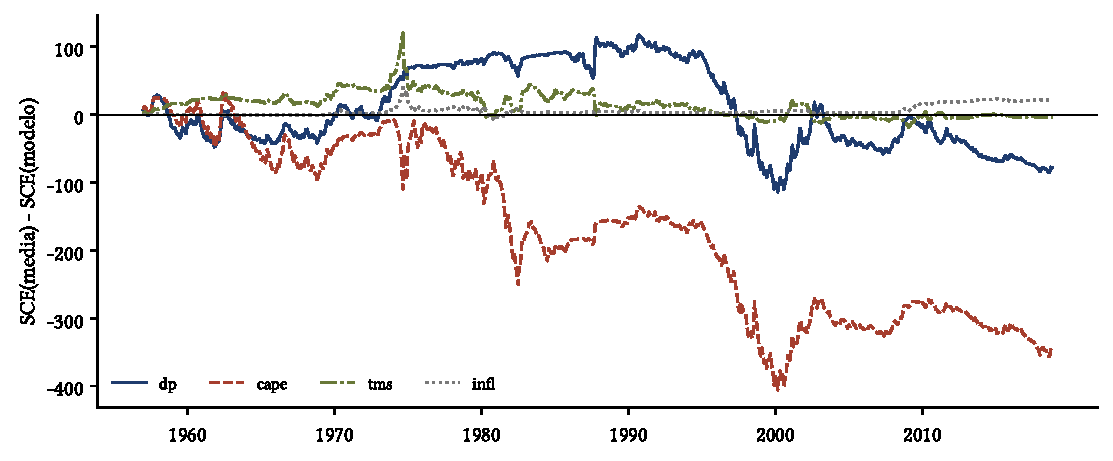
\includegraphics[width=\linewidth]{graficos/cap20_ej01_goyal_welch.pdf}
\caption{Diferencia acumulada entre el error cuadrático de la media histórica y el de cada modelo univariado. Una curva creciente
indica que el modelo gana.}
\label{fig:goyalwelch}
\end{figure}

\begin{conclusion}
La significancia dentro de la muestra no garantiza capacidad predictiva fuera de ella. Los predictores clásicos de la prima de mercado
pronostican, en el mejor de los casos, apenas mejor que la media.
\end{conclusion}
\end{ejresuelto}

\begin{ejresuelto}{Todos los predictores con contracción}\label{ej:contraccion}
\enunciado Use todos los predictores a la vez con MCO, ridge, red elástica ($\alpha=0{,}5$) y lasso, reestimando cada enero desde 1957. Elija
$\lambda$ en una malla de 30 valores con los últimos 120 meses de cada muestra de entrenamiento.

\solucion
\paso{Paso 1. Colinealidad exacta.} $de=dp-ep$ y $tms=lty-tbl$ son combinaciones lineales exactas de otros predictores: con los diez,
$X'X$ es singular y MCO no tiene solución única. R lo detecta (``system is computationally singular''); Python, por redondeo, devolvía
un resultado sin advertir. Usamos ocho predictores.

\paso{Paso 2. Resultados.}
\begin{center}\small
\begin{tabular}{@{}lrrrr@{}}
\toprule
Modelo & $R^2_{OS}$ (\%) & $R^2_{OS}$ CT (\%) & $p$ (CW) & $\lambda$ mediano \\
\midrule
MCO (8 predictores) & $-6{,}04$ & $-2{,}93$ & 0,531 & -- \\
Ridge & $-1{,}12$ & 0,17 & 0,370 & 3,324 \\
Red elástica & $-2{,}33$ & $-0{,}94$ & 0,692 & 0,846 \\
Lasso & $-1{,}95$ & $-0{,}90$ & 0,605 & 0,499 \\
\bottomrule
\end{tabular}
\end{center}
MCO con todos los predictores es desastroso: $R^2_{OS}=-6{,}04$\,\%. Sus pronósticos tienen una desviación estándar de 1,01\,\% mensual, doce
veces la de la media histórica (0,08\,\%): reacciona con fuerza a variaciones de los predictores que solo son ruido. La contracción
reduce esa volatilidad (0,44 con ridge, 0,52 con lasso) y el error, pero no lo suficiente para superar a la media.

\paso{Paso 3. Qué selecciona el lasso.} En promedio, 2,56 predictores; en 14 de las 62 reestimaciones, ninguno (el pronóstico es la
media). El CAPE entra en el 77\,\% de las reestimaciones, el momentum en el 42\,\% y la volatilidad apenas en el 6\,\% (Figura~\ref{fig:contraccion}).

\codigoweb{cap20_ej02}
\salidaR{cap20_ej02_R.txt}
\lectura{cap20_ej02}

\RvsPy El descenso por coordenadas está programado igual en ambos lenguajes, con la misma tolerancia y arranque en caliente a lo largo
de la malla de $\lambda$ (cada ajuste parte de la solución del $\lambda$ anterior). Los predictores se estandarizan con la media y la
desviación estándar de la muestra de entrenamiento (dividiendo entre $n$), nunca con la de toda la muestra. Los paquetes de referencia son
\texttt{glmnet} en R y \texttt{sklearn.linear\_model.ElasticNet} en Python, que parametrizan la penalización de la misma forma; el bucle en
Python tarda unos dos minutos, frente a 30 segundos en R.

\begin{figure}[ht]
\centering
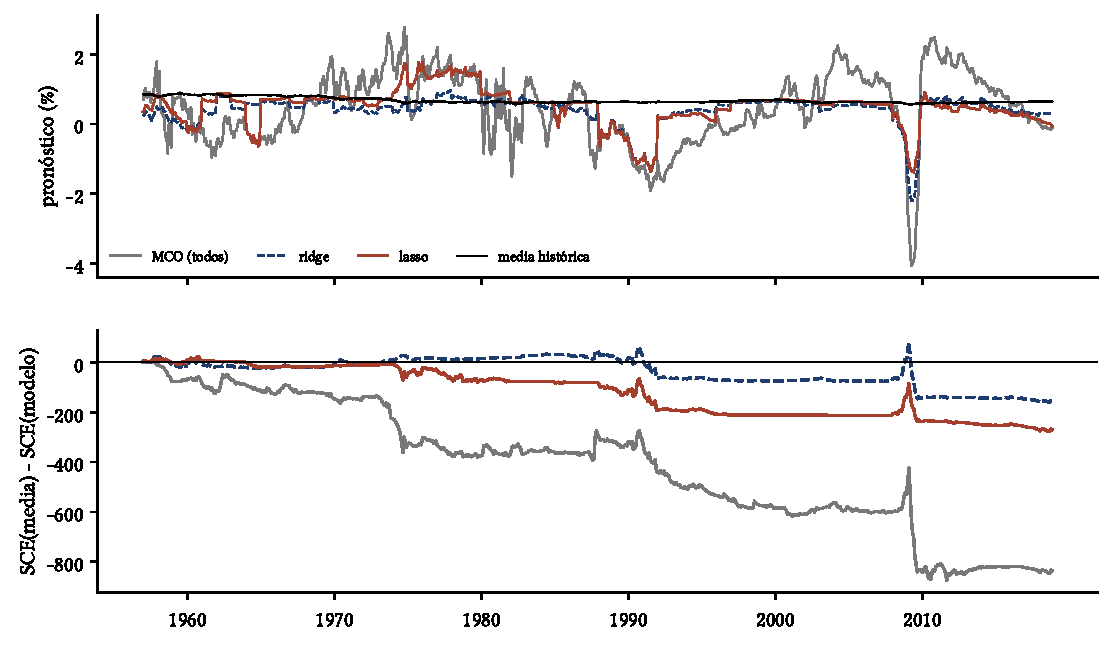
\includegraphics[width=\linewidth]{graficos/cap20_ej02_contraccion.pdf}
\caption{Arriba: pronósticos mensuales de MCO, ridge, lasso y la media histórica. Abajo: diferencia acumulada de errores cuadráticos
frente a la media.}
\label{fig:contraccion}
\end{figure}

\begin{conclusion}
Con una señal tan débil, más variables empeoran el pronóstico, y la contracción solo atenúa el daño. La validación temporal elige
penalizaciones altas, es decir, pronósticos cercanos a la media: los datos le dicen al algoritmo que confíe poco en los predictores.
\end{conclusion}
\end{ejresuelto}

\begin{ejresuelto}{Combinación de pronósticos y su valor económico}\label{ej:combinacion}
\enunciado Combine los diez pronósticos univariados del Ejercicio~\ref{ej:goyalwelch} con su media y su mediana (Rapach, Strauss y Zhou, 2010) y
compare con regresiones sobre 1, 2 y 3 componentes principales. Evalúe el valor económico para un inversionista media-varianza con aversión 3.

\solucion
\paso{Paso 1. Precisión.}
\begin{center}\small
\begin{tabular}{@{}lrrr@{}}
\toprule
Modelo & $R^2_{OS}$ (\%) & CW & $p$ \\
\midrule
Combinación (media) & 0,61 & 2,13 & 0,017 \\
Combinación (mediana) & 0,50 & 2,29 & 0,011 \\
Componentes principales ($k=1$) & $-0{,}36$ & 2,16 & 0,016 \\
Componentes principales ($k=2$) & $-0{,}78$ & 2,19 & 0,014 \\
Componentes principales ($k=3$) & $-1{,}53$ & 2,04 & 0,021 \\
\bottomrule
\end{tabular}
\end{center}
La media simple de los diez pronósticos, ninguno de los cuales supera claramente a la media histórica, tiene $R^2_{OS}=0{,}61$\,\% y
supera a la media con $p=0{,}017$. La combinación es una forma extrema de contracción: cada predictor recibe un peso fijo de 1/10, sin
estimar, y los errores de los distintos modelos se compensan. Su desviación estándar es 0,11\,\%, apenas mayor que la de la media
histórica (Figura~\ref{fig:combinacion}).

\paso{Paso 2. Valor económico.} El inversionista invierte en acciones $w_t=\hat y_{t+1}/(\gamma\hat\sigma^2_t)$, con $\gamma=3$, la varianza de los
últimos 60 meses y el peso acotado entre 0 y 150\,\%. Su equivalente cierto anual es
\begin{align*}
  EC &= 12\Bigl[\bar r_p-\tfrac{\gamma}{2}\hat\sigma^2_p\Bigr],\\
  EC_{\text{combinación}}-EC_{\text{media}} &= 7{,}570-6{,}617\\
                                            &= 0{,}953\ \text{puntos porcentuales por año}.
\end{align*}
Casi un punto anual: el inversionista pagaría hasta 0,95\,\% de su patrimonio cada año por usar la combinación. Con solo $dp$, en cambio,
pierde 0,88 puntos.

\codigoweb{cap20_ej03}
\salidaR{cap20_ej03_R.txt}
\lectura{cap20_ej03}

\RvsPy Con rendimientos en porcentaje, el peso óptimo es $100\,\hat y/(\gamma\hat\sigma^2)$ y la penalización por varianza se divide entre 100; una
primera versión del código olvidó esas escalas y daba equivalentes ciertos absurdos de más de 400\,\% anual. Los autovectores de
\texttt{eigen} (R) y \texttt{np.linalg.eigh} (Python) pueden tener signos opuestos, pero eso no cambia la regresión sobre los componentes.

\begin{figure}[ht]
\centering
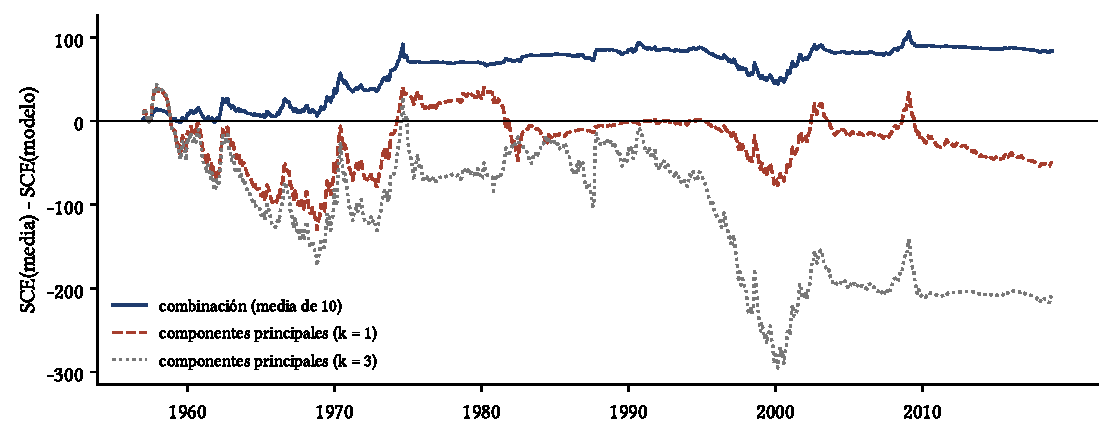
\includegraphics[width=\linewidth]{graficos/cap20_ej03_combinacion.pdf}
\caption{Diferencia acumulada de errores cuadráticos frente a la media histórica de la combinación y de las regresiones sobre componentes
principales.}
\label{fig:combinacion}
\end{figure}

\begin{conclusion}
El mejor ``modelo'' no es el más sofisticado sino el más humilde: promediar pronósticos simples. Y un $R^2_{OS}$ de 0,6\,\% vale casi un punto
porcentual anual para un inversionista, como anticipa la Proposición~\ref{prop:ct}.
\end{conclusion}
\end{ejresuelto}

\begin{ejresuelto}{¿Anuncia la curva las recesiones?}\label{ej:recesiones20}
\enunciado Con los datos de 1946 a 1991, estime un logit de la probabilidad de que el mes $t+h$ esté en recesión según la pendiente de la curva
$y_{120}-y_3$ en $t$, para $h=3$, 6, 12, 18 y 24 meses. Para $h=12$, calcule la tabla de clasificación con dos umbrales y la AUC fuera de
muestra desde 1965.

\solucion
\paso{Paso 1. Horizontes.}
\begin{center}\small
\begin{tabular}{@{}rrrrr@{}}
\toprule
$h$ & $\hat\beta_1$ & ee & Pseudo $R^2$ & AUC \\
\midrule
3 & $-0{,}576$ & 0,108 & 0,063 & 0,660 \\
6 & $-0{,}930$ & 0,127 & 0,141 & 0,752 \\
12 & $-1{,}174$ & 0,145 & 0,199 & 0,819 \\
18 & $-0{,}718$ & 0,114 & 0,095 & 0,715 \\
24 & $-0{,}237$ & 0,100 & 0,011 & 0,557 \\
\bottomrule
\end{tabular}
\end{center}
La pendiente predice mejor a un año: es el resultado de Estrella y Mishkin (1998). Agregar el nivel de la tasa corta no ayuda ($LR=0{,}17$).

\paso{Paso 2. Probabilidades.} Con $\hat\beta_0=-0{,}695$ y $\hat\beta_1=-1{,}174$:
\begin{align*}
  \Pr(\text{recesión}\mid\text{pendiente}=0) &= \frac{1}{1+e^{0{,}695}}\\
                                            &= 0{,}333,\\
  \Pr(\text{recesión}\mid\text{pendiente}=2) &= \frac{1}{1+e^{0{,}695+2\times1{,}174}}\\
                                            &= \frac{1}{1+e^{3{,}043}}\\
                                            &= 0{,}046 .
\end{align*}
La probabilidad supera el 50\,\% solo cuando la curva está invertida en más de 0,59 puntos.

\paso{Paso 3. Umbrales.} Con umbral 0,5, el modelo detecta solo 23 de 95 meses de recesión (sensibilidad 0,24) con pocas falsas alarmas
(especificidad 0,97). Con umbral igual a la frecuencia muestral (0,183), detecta 71 (sensibilidad 0,75) a costa de 112 falsas alarmas
(especificidad 0,74). La AUC resume todos los umbrales: 0,819 dentro de la muestra y 0,835 fuera de muestra desde 1965, usando solo
recesiones ya observadas en cada fecha (Figura~\ref{fig:recesiones20}).

\codigoweb{cap20_ej04}
\salidaR{cap20_ej04_R.txt}
\lectura{cap20_ej04}

\RvsPy Newton-Raphson está programado en ambos lenguajes; \texttt{glm(..., family = binomial)} en R y \texttt{statsmodels.Logit} en Python dan los
mismos coeficientes. La AUC usa los rangos promedio, de modo que los empates cuentan un medio. En el ejercicio fuera de muestra se supone
que el estado de la economía se conoce de inmediato; en la práctica el NBER fecha las recesiones con meses o años de retraso, lo que hace la
evaluación algo optimista.

\begin{figure}[ht]
\centering
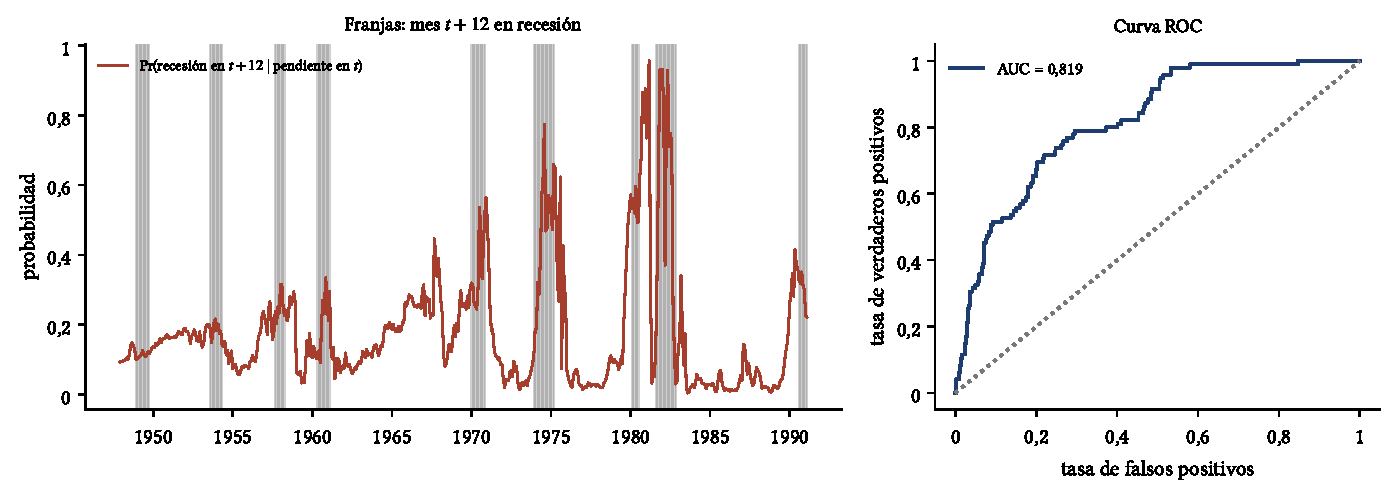
\includegraphics[width=\linewidth]{graficos/cap20_ej04_recesiones.pdf}
\caption{Izquierda: probabilidad estimada de recesión 12 meses después, con las franjas grises en los meses $t+12$ que estuvieron en recesión.
Derecha: curva ROC dentro de la muestra.}
\label{fig:recesiones20}
\end{figure}

\begin{conclusion}
Una sola variable financiera, la pendiente de la curva, clasifica bien las recesiones de un año después. El umbral de decisión depende del
costo relativo de una falsa alarma y de una recesión no anticipada, y la AUC permite comparar modelos sin elegirlo.
\end{conclusion}
\end{ejresuelto}

\begin{ejresuelto}{Árboles y sobreajuste}\label{ej:arboles}
\enunciado Entrene árboles de regresión de profundidad 0 a 6 (hojas de al menos 24 meses) con los ocho predictores de 1927 a 1980, y evalúelos en
1981--2018. Compare con MCO.

\solucion
\paso{Paso 1. Entrenamiento frente a prueba.}
\begin{center}\small
\begin{tabular}{@{}rrrrr@{}}
\toprule
Profundidad & Hojas & ECM entrenamiento & ECM prueba & $R^2$ prueba (\%) \\
\midrule
0 & 1 & 35,56 & 18,83 & 0,00 \\
1 & 2 & 34,01 & 20,83 & $-10{,}59$ \\
2 & 3 & 33,02 & 20,77 & $-10{,}29$ \\
4 & 6 & 31,99 & 20,94 & $-11{,}22$ \\
6 & 10 & 31,05 & 23,11 & $-22{,}70$ \\
\bottomrule
\end{tabular}
\end{center}
Cada corte reduce el error de entrenamiento y aumenta el de prueba. El mejor árbol es el que no corta nada, es decir, la media
(Figura~\ref{fig:arboles}). MCO lineal con los ocho predictores también pierde frente a la media: $R^2=-7{,}79$\,\%.

\paso{Paso 2. Qué aprende el árbol.} El de profundidad 2 separa 24 meses con CAPE muy bajo ($\ln\text{CAPE}\le2{,}18$, un CAPE menor que 8,8),
con un exceso de rendimiento medio de 6,95\,\% mensual, y 28 meses con deflación fuerte (inflación rezagada menor que $-3{,}44$\,\%), con
$-4{,}26$\,\%. Los primeros son meses de 1932--1933, 1942, 1974 y 1979--1980; los segundos, de 1930--1933 y 1938. Con 640 meses, el árbol
aísla unos pocos episodios extraordinarios, sobre todo de la Gran Depresión, que no se repitieron después de 1980.

\codigoweb{cap20_ej05}
\salidaR{cap20_ej05_R.txt}
\lectura{cap20_ej05}

\RvsPy El árbol se construye recursivamente en ambos lenguajes con una búsqueda exhaustiva de cortes en los puntos medios entre valores
consecutivos; los ordenamientos estables (\texttt{order(..., method = "radix")} y \texttt{np.argsort(..., kind = "stable")}) garantizan los mismos
desempates. Los paquetes de referencia (\texttt{rpart}, \texttt{sklearn.tree}) agregan poda por complejidad y validación cruzada, que aquí haría
lo mismo que la tabla: elegir la profundidad cero.

\begin{figure}[ht]
\centering
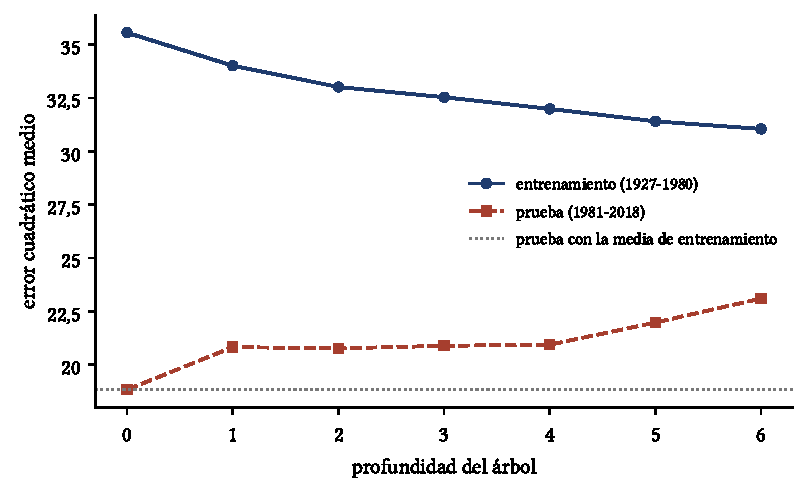
\includegraphics[width=0.78\linewidth]{graficos/cap20_ej05_arboles.pdf}
\caption{Error cuadrático medio de árboles de profundidad creciente en el período de entrenamiento y en el de prueba.}
\label{fig:arboles}
\end{figure}

\begin{conclusion}
Los métodos flexibles necesitan muchos datos y una señal estable. Con la prima de mercado agregada no hay ninguna de las dos cosas, y un árbol
solo memoriza la historia. En el corte transversal de miles de acciones, con millones de observaciones, los mismos métodos sí encuentran
estructura (Gu, Kelly y Xiu, 2020).
\end{conclusion}
\end{ejresuelto}

% ---------------------------------------------------------------------
\section{Ejercicios propuestos}
% ---------------------------------------------------------------------

\begin{enumerate}[label=\textbf{\thechapter.\arabic*},leftmargin=*,itemsep=6pt]
  \item Con regresores ortonormales, $\hat\beta=(2{,}0;\,0{,}5;\,-1{,}2)$ y $\lambda=0{,}8$, calcule ridge y lasso. \textit{Respuesta: ridge
  $(1{,}111;\,0{,}278;\,-0{,}667)$; lasso $(1{,}2;\,0;\,-0{,}4)$.}

  \item Con $S=0{,}12$ mensual y $R^2=1$\,\%, ¿en qué proporción aumenta el rendimiento esperado del inversionista de la Proposición~\ref{prop:ct}?
  \textit{Respuesta: $(0{,}0144+0{,}01)/0{,}99/0{,}0144-1=0{,}71$, un 71\,\%.}

  \item Un logit tiene $\beta_0=-0{,}7$ y $\beta_1=-1{,}2$. Calcule la probabilidad con $x=-1$ y el efecto marginal en ese punto.
  \textit{Respuesta: $p=1/(1+e^{-0{,}5})=0{,}622$; $\beta_1p(1-p)=-0{,}282$.}

  \item Demuestre que la AUC calculada con rangos es igual a la proporción de pares (positivo, negativo) en que el positivo tiene mayor puntaje.

  \item Demuestre que con $X'X/n=I$ la red elástica es $S(\hat\beta_j,\lambda\alpha)/(1+\lambda(1-\alpha))$.

  \item \emph{(Simulación.)} Genere 1\,000 meses de $y_{t+1}=0{,}1x_t+\varepsilon_{t+1}$ con $x$ AR(1) de persistencia 0,98 y $R^2=0{,}5$\,\%, y 20 predictores
  irrelevantes. Compare el $R^2_{OS}$ de MCO, lasso y la combinación.

  \item \emph{(Con datos del BCRP.)} Prediga la dirección del tipo de cambio sol-dólar del mes siguiente con un logit y diferenciales de tasas,
  y evalúe la AUC fuera de muestra.

  \item \emph{(Con datos.)} Repita el Ejercicio~\ref{ej:goyalwelch} empezando la evaluación en 1990. ¿Cambia el ranking de predictores?
\end{enumerate}

% ---------------------------------------------------------------------
\section{Resumen de fórmulas}
% ---------------------------------------------------------------------

\begin{table}[H]
\centering\small
\begin{tabular}{@{}ll@{}}
\toprule
Concepto & Fórmula \\
\midrule
Sesgo y varianza & $\E[(y_0-\hat f)^2]=\sigma^2+\text{sesgo}^2+\Var(\hat f)$ \\
Red elástica & $\frac1{2n}\lVert\mathbf y-X\boldsymbol\beta\rVert^2+\lambda[\alpha\lVert\boldsymbol\beta\rVert_1+\frac{1-\alpha}{2}\lVert\boldsymbol\beta\rVert_2^2]$ \\
Ortonormal & ridge $\hat\beta/(1+\lambda)$;\quad lasso $\operatorname{signo}(\hat\beta)\max(|\hat\beta|-\lambda,0)$ \\
Descenso por coordenadas & $\beta_j\leftarrow S(\mathbf x_j'\mathbf r_{-j}/n,\lambda\alpha)/(1+\lambda(1-\alpha))$ \\
$R^2$ fuera de muestra & $1-\sum(y-\hat y)^2/\sum(y-\bar y)^2$ \\
Clark y West & $f=(y-\bar y)^2-[(y-\hat y)^2-(\bar y-\hat y)^2]$;\quad $t$ de $\bar f$ \\
Valor de un $R^2$ & $\frac{S^2+R^2}{\gamma(1-R^2)}$ frente a $\frac{S^2}{\gamma}$ \\
Logit & $p=1/(1+e^{-\mathbf x'\boldsymbol\beta})$;\quad $\nabla\ell=X'(\mathbf y-\mathbf p)$;\quad $\nabla^2\ell=-X'WX$ \\
AUC & $\Pr(\text{puntaje de un positivo}>\text{puntaje de un negativo})$ \\
\bottomrule
\end{tabular}
\caption{Fórmulas principales del Capítulo 20.}
\end{table}

\section*{Referencias}
\begin{itemize}[leftmargin=*]
  \item Breiman, L., Friedman, J., Olshen, R. y Stone, C. (1984). \emph{Classification and Regression Trees}. Wadsworth.
  \item Campbell, J. Y. y Thompson, S. B. (2008). Predicting excess stock returns out of sample: Can anything beat the historical average?
        \emph{Review of Financial Studies}, 21(4), 1509--1531.
  \item Clark, T. E. y West, K. D. (2007). Approximately normal tests for equal predictive accuracy in nested models. \emph{Journal of
        Econometrics}, 138(1), 291--311.
  \item Estrella, A. y Mishkin, F. S. (1998). Predicting U.S. recessions: Financial variables as leading indicators. \emph{Review of
        Economics and Statistics}, 80(1), 45--61.
  \item Friedman, J., Hastie, T. y Tibshirani, R. (2010). Regularization paths for generalized linear models via coordinate descent.
        \emph{Journal of Statistical Software}, 33(1), 1--22.
  \item Goyal, A. y Welch, I. (2008). A comprehensive look at the empirical performance of equity premium prediction. \emph{Review of
        Financial Studies}, 21(4), 1455--1508.
  \item Gu, S., Kelly, B. y Xiu, D. (2020). Empirical asset pricing via machine learning. \emph{Review of Financial Studies}, 33(5),
        2223--2273.
  \item Hastie, T., Tibshirani, R. y Friedman, J. (2009). \emph{The Elements of Statistical Learning}, 2.ª ed. Springer.
  \item Hoerl, A. E. y Kennard, R. W. (1970). Ridge regression: Biased estimation for nonorthogonal problems. \emph{Technometrics}, 12(1),
        55--67.
  \item Rapach, D. E., Strauss, J. K. y Zhou, G. (2010). Out-of-sample equity premium prediction: Combination forecasts and links to the real
        economy. \emph{Review of Financial Studies}, 23(2), 821--862.
  \item Tibshirani, R. (1996). Regression shrinkage and selection via the lasso. \emph{Journal of the Royal Statistical Society, Series B},
        58(1), 267--288.
  \item Zou, H. y Hastie, T. (2005). Regularization and variable selection via the elastic net. \emph{Journal of the Royal Statistical
        Society, Series B}, 67(2), 301--320.
\end{itemize}

% =====================================================================
%  Capítulo 21. Proyecto integrador
% =====================================================================
\chapter[Proyecto integrador]{Proyecto integrador: riesgo y asignación de una cartera de acciones tecnológicas}\label{cap:proyecto}

\section*{Objetivos de aprendizaje}
Al terminar este capítulo, el lector podrá:
\begin{enumerate}[label=\arabic*.,leftmargin=*]
  \item Organizar un análisis econométrico financiero completo, de la pregunta al informe, con código reproducible en
        R y en Python.
  \item Encadenar los métodos del libro: hechos estilizados, modelos de factores, volatilidad condicional, medidas de
        riesgo y asignación de cartera.
  \item Separar con rigor la estimación de la evaluación fuera de muestra y reconocer los sesgos que invalidan un
        análisis: la información del futuro, la selección de la muestra y las pruebas múltiples.
  \item Redactar conclusiones que distingan lo que los datos muestran de lo que no pueden mostrar.
\end{enumerate}

\section*{Motivación}
Los capítulos anteriores presentaron cada método por separado. En la práctica, un analista recibe una pregunta y debe
decidir qué métodos usar, en qué orden y cómo evaluar el resultado. Este capítulo resuelve un caso completo: un comité de
inversiones considera una cartera de cuatro grandes acciones tecnológicas estadounidenses y pide responder cinco preguntas.
¿Cómo se comportan sus rendimientos? ¿Cuánto riesgo de mercado agregan? ¿Cómo pronosticar su volatilidad? ¿Cuánto puede
perder la cartera en un mal día, y son confiables esas cifras? ¿Conviene ponderar por igual o minimizar la varianza?

\paragraph{Datos del capítulo.} Precios de cierre diarios ajustados de Apple (AAPL), Amazon (AMZN), Facebook (FB) y
Alphabet (GOOG), y el índice S\&P 500, del 2 de enero de 2014 al 31 de diciembre de 2018 (1\,257 rendimientos diarios), los
mismos del Capítulo~\ref{cap:eventos}. El índice es de precios: no incluye dividendos.

% ---------------------------------------------------------------------
\section{Un flujo de trabajo reproducible}
% ---------------------------------------------------------------------

Un proyecto empírico sigue cinco pasos, y cada uno tiene un error típico que el libro ha señalado.
\begin{enumerate}[label=\arabic*.,leftmargin=*]
  \item \textbf{Pregunta y datos.} Definir qué decisión informa el análisis y qué datos la responden. Documentar la fuente, la
        fecha de descarga y cada transformación (el archivo \texttt{FUENTES.txt} del proyecto). \emph{Error típico}: usar datos
        con sesgo de supervivencia o sin ajustar por dividendos y divisiones.
  \item \textbf{Diagnóstico.} Describir los datos antes de modelarlos: momentos, colas, autocorrelación de los rendimientos y de sus
        cuadrados. \emph{Error típico}: suponer normalidad o independencia sin verificarlas.
  \item \textbf{Modelo y estimación.} Elegir el modelo más simple que capture los rasgos encontrados y estimarlo con datos de una
        ventana de estimación. \emph{Error típico}: elegir el modelo después de ver su desempeño en los datos de evaluación.
  \item \textbf{Evaluación fuera de muestra.} Medir el desempeño con datos que no intervinieron en la estimación ni en la elección
        del modelo, con las pruebas adecuadas (Kupiec y Christoffersen para el VaR; Diebold-Mariano para pronósticos). \emph{Error
        típico}: usar en el pronóstico de $t$ información posterior a $t$.
  \item \textbf{Informe.} Responder la pregunta con cifras, incertidumbre y limitaciones. \emph{Error típico}: informar solo
        los resultados significativos.
\end{enumerate}
La Figura~\ref{fig:flujo} muestra cómo se encadenan las cinco etapas del proyecto y qué capítulos usa cada una. Todo el código
reutiliza las funciones ya escritas: \texttt{cap08\_funciones} para el GARCH y \texttt{cap13\_funciones} para el VaR, el ES y las
pruebas retrospectivas.

\begin{figure}[ht]
\centering
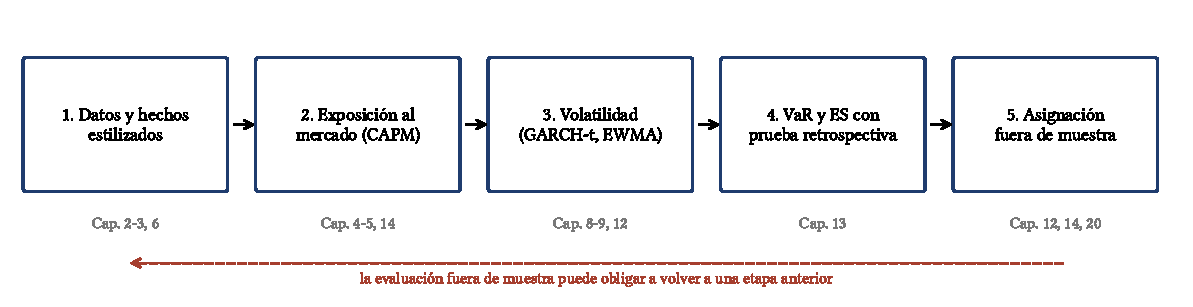
\includegraphics[width=\linewidth]{graficos/cap21_fig_flujo.pdf}
\caption{Etapas del proyecto integrador y capítulos del libro que usa cada una.}
\label{fig:flujo}
\end{figure}

% ---------------------------------------------------------------------
\section{Herramientas adicionales para el proyecto}
% ---------------------------------------------------------------------

La primera herramienta es la cartera de mínima varianza global de la Proposición~\ref{prop:minvar} (Capítulo~\ref{cap:dcc}):
\[
  \mathbf w^*=\frac{\Sigma^{-1}\mathbf 1}{\mathbf 1'\Sigma^{-1}\mathbf 1},\qquad \sigma^2_{\min}=\frac{1}{\mathbf 1'\Sigma^{-1}\mathbf 1}.
\]

La cartera de mínima varianza solo necesita covarianzas, no medias, y por eso se estima mejor que la cartera tangente: los
rendimientos esperados son la parte más ruidosa (Merton, 1980). Aun así, con $\Sigma$ estimada, $\mathbf w^*$ hereda el error de
estimación. DeMiguel, Garlappi y Uppal (2009) mostraron que la regla ingenua $1/N$, que no estima nada, es difícil de superar
fuera de muestra.

\begin{proposicion}[Error estándar de la razón de Sharpe]\label{prop:sesharpe}
Si los rendimientos son i.i.d.\ normales con media $\mu$ y desviación $\sigma$, la razón de Sharpe muestral
$\widehat{SR}=\bar r/\hat\sigma$ con $T$ observaciones cumple, aproximadamente,
\[
  \Var(\widehat{SR})\approx\frac{1}{T}\Bigl(1+\frac{SR^2}{2}\Bigr).
\]
\end{proposicion}

\begin{proof}
Con normalidad, $\bar r$ y $\hat\sigma^2$ son independientes, $\Var(\bar r)=\sigma^2/T$ y $\Var(\hat\sigma^2)\approx2\sigma^4/T$. Por el método delta,
con $g(m,v)=m/\sqrt v$, $\partial g/\partial m=1/\sigma$ y $\partial g/\partial v=-\mu/(2\sigma^3)$:
\begin{align*}
  \Var(\widehat{SR}) &\approx \Bigl(\frac1\sigma\Bigr)^2\frac{\sigma^2}{T}+\Bigl(\frac{\mu}{2\sigma^3}\Bigr)^2\frac{2\sigma^4}{T}\\
                     &= \frac1T+\frac{\mu^2}{4\sigma^6}\cdot\frac{2\sigma^4}{T}\\
                     &= \frac1T+\frac{\mu^2}{2\sigma^2T}\\
                     &= \frac1T\Bigl(1+\frac{SR^2}{2}\Bigr).
\end{align*}
\end{proof}

Con datos diarios, $SR$ es pequeño y el error estándar es casi $1/\sqrt T$. Anualizado (multiplicando por $\sqrt{252}$), con cuatro años de
datos es cercano a $\sqrt{252/1\,007}=0{,}50$: una razón de Sharpe anual de 1 no es distinguible de 0 con 95\,\% de confianza (Lo, 2002).

\begin{proposicion}[Pruebas múltiples]\label{prop:multiples}
Si se prueban $K$ hipótesis nulas verdaderas e independientes, cada una al nivel $\alpha$, la probabilidad de al menos un rechazo es
$1-(1-\alpha)^K$. Con la corrección de Bonferroni (nivel $\alpha/K$ en cada prueba) esa probabilidad es como máximo $\alpha$.
\end{proposicion}

\begin{proof}
La probabilidad de no rechazar ninguna es el producto de las de no rechazar cada una:
\begin{align*}
  \Pr(\text{ningún rechazo}) &= \prod_{k=1}^K(1-\alpha)\\
                             &= (1-\alpha)^K,\\
  \Pr(\text{al menos uno}) &= 1-(1-\alpha)^K .
\end{align*}
Para Bonferroni, por la desigualdad de Boole y sin necesidad de independencia:
\begin{align*}
  \Pr\Bigl(\bigcup_k\{\text{rechazo }k\}\Bigr) &\le \sum_{k=1}^K\Pr(\text{rechazo }k)\\
                                             &= K\cdot\frac{\alpha}{K}\\
                                             &= \alpha .
\end{align*}
\end{proof}

Con 20 estrategias sin valor, cada una al 5\,\%, la probabilidad de encontrar al menos una ``significativa'' es $1-0{,}95^{20}=0{,}64$. Es el
problema de la minería de datos (Harvey, Liu y Zhu, 2016). Un caso extremo es la \emph{selección de la muestra}: elegir hoy los activos que
mejor rindieron en el pasado garantiza que su rendimiento pasado parezca extraordinario.

% ---------------------------------------------------------------------
\section{El proyecto, etapa por etapa}
% ---------------------------------------------------------------------

\begin{ejresuelto}{Etapa 1: los datos y sus hechos estilizados}\label{ej:etapa1}
\enunciado Describa los cinco rendimientos diarios: media y volatilidad anualizadas, asimetría, curtosis, prueba de Jarque-Bera,
Ljung-Box de 10 rezagos para los rendimientos y sus cuadrados, peor día y correlaciones.

\solucion
\paso{Paso 1. Momentos.}
\begin{center}\small
\begin{tabular}{@{}lrrrrrrr@{}}
\toprule
Serie & Media anual & Vol.\ anual & Asimetría & Curtosis & JB & LB($r^2$) & Peor día \\
\midrule
AAPL & 19,99 & 24,04 & $-0{,}05$ & 6,67 & 707 & 52,9 & $-7{,}99$ \\
AMZN & 31,41 & 30,99 & 0,50 & 12,55 & 4\,824 & 22,9 & $-11{,}00$ \\
FB & 22,02 & 29,92 & $-0{,}18$ & 18,21 & 12\,125 & 11,5 & $-18{,}96$ \\
GOOG & 15,31 & 23,45 & 0,96 & 15,96 & 8\,990 & 17,1 & $-5{,}32$ \\
S\&P 500 & 7,16 & 13,23 & $-0{,}43$ & 6,74 & 770 & 386,0 & $-4{,}10$ \\
\bottomrule
\end{tabular}
\end{center}
Todas las series rechazan la normalidad con holgura (valor crítico de JB al 1\,\%: 9,21). Ninguna tiene autocorrelación significativa al 1\,\% en los
rendimientos (valor crítico 23,21). En los cuadrados, el S\&P 500 (386,0) y Apple (52,9) muestran un agrupamiento de volatilidad muy fuerte; Facebook
no (11,5): sus días extremos son saltos aislados por noticias propias, como la caída del 26 de julio de 2018 del Capítulo~\ref{cap:eventos}.

\paso{Paso 2. Dependencia.} Las correlaciones entre las acciones van de 0,40 (AAPL-FB) a 0,62 (AMZN-GOOG), y con el S\&P 500, de 0,56 a 0,67
(Figura~\ref{fig:riqueza}).

\paso{Paso 3. Una advertencia sobre la muestra.} Estas cuatro empresas se eligen hoy porque fueron las grandes ganadoras de la década: con
medias anuales de 15 a 31\,\%, frente a 7\,\% del índice. Cualquier conclusión sobre su rendimiento medio tiene \emph{sesgo de selección}. Por eso
el proyecto se concentra en el riesgo, que depende de varianzas y correlaciones y es mucho menos sensible a esa elección.

\codigoweb{cap21_ej01}
\salidaR{cap21_ej01_R.txt}
\lectura{cap21_ej01}

\RvsPy El archivo de funciones del proyecto importa las de los Capítulos 8 y 13 (\texttt{source} en R, \texttt{from ... import} en Python), de modo que el
GARCH y las pruebas retrospectivas son exactamente las ya verificadas. El estadístico de Ljung-Box se programa directamente para controlar la
definición de las autocorrelaciones.

\begin{figure}[ht]
\centering
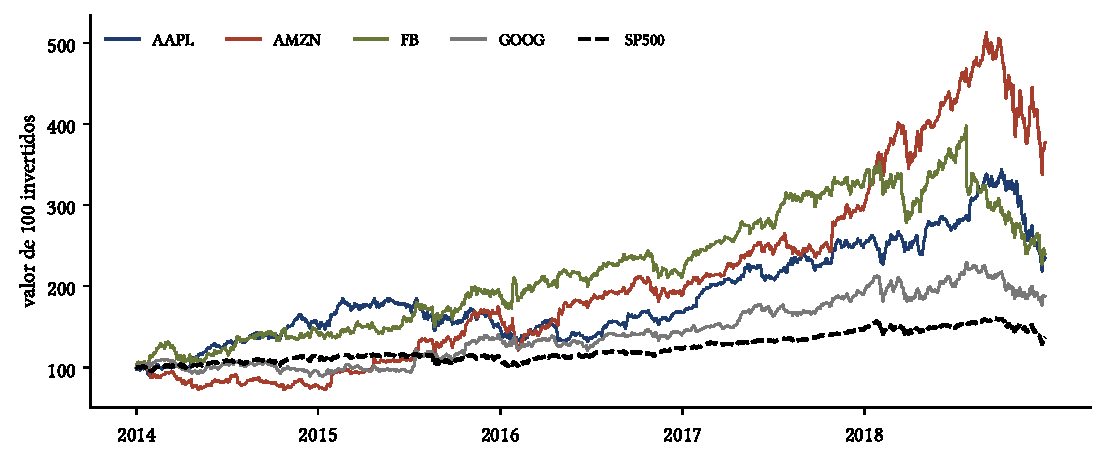
\includegraphics[width=\linewidth]{graficos/cap21_ej01_riqueza.pdf}
\caption{Valor de 100 invertidos en cada acción y en el S\&P 500 a inicios de 2014.}
\label{fig:riqueza}
\end{figure}

\begin{conclusion}
Los rendimientos tienen colas mucho más pesadas que la normal, no son predecibles en media y, salvo Facebook, muestran agrupamiento de volatilidad. Los
modelos de riesgo deben incorporar ambos rasgos.
\end{conclusion}
\end{ejresuelto}

\begin{ejresuelto}{Etapa 2: exposición al mercado}\label{ej:etapa2}
\enunciado Estime el CAPM diario de cada acción y de la cartera 1/N con el S\&P 500 como mercado y errores de Newey-West de 5 rezagos.

\solucion
\paso{Paso 1. Betas y alfas.}
\begin{center}\small
\begin{tabular}{@{}lrrrrr@{}}
\toprule
Acción & Alfa anual (\%) & $t$(alfa) & Beta & $t$(beta $=1$) & $R^2$ \\
\midrule
AAPL & 11,91 & 1,34 & 1,127 & 2,88 & 0,384 \\
AMZN & 21,79 & 1,96 & 1,343 & 4,36 & 0,329 \\
FB & 13,03 & 1,23 & 1,255 & 4,79 & 0,308 \\
GOOG & 6,78 & 0,89 & 1,190 & 4,55 & 0,451 \\
Cartera 1/N & 13,38 & 2,23 & 1,229 & -- & 0,566 \\
\bottomrule
\end{tabular}
\end{center}
Las cuatro betas son significativamente mayores que 1: la cartera amplifica los movimientos del mercado en un 23\,\%. La beta de la cartera es el promedio
de las betas, como debe ser por linealidad. Entre el 55 y el 69\,\% de la varianza de cada acción es idiosincrática, y la diversificación entre solo cuatro
acciones la reduce: el $R^2$ de la cartera sube a 0,57.

\paso{Paso 2. El alfa.} El alfa de la cartera, 13,4\,\% anual con $t=2{,}23$, sería significativo al 5\,\% si fuera la única prueba. Pero con cinco pruebas
(Proposición~\ref{prop:multiples}) el nivel de Bonferroni es $0{,}05/5=0{,}01$, y sobre todo la muestra se eligió por su rendimiento pasado: el alfa es,
en buena medida, el sesgo de selección de la Etapa 1. No es una predicción.

\paso{Paso 3. Estabilidad.} La beta de la cartera sube de 1,185 en 2014--2015 a 1,261 en 2016--2018.

\codigoweb{cap21_ej02}
\salidaR{cap21_ej02_R.txt}
\lectura{cap21_ej02}

\RvsPy Usamos rendimientos totales en lugar de excesos: la tasa libre de riesgo diaria entre 2014 y 2018 fue de pocas milésimas de punto porcentual y no
altera las betas. Los errores de Newey-West usan la función \texttt{nw\_mco} del proyecto, la misma fórmula del Capítulo~\ref{cap:robustos}.

\begin{conclusion}
La cartera es un instrumento de mercado amplificado: su riesgo está dominado por el del mercado (beta de 1,23) y la diversificación entre cuatro acciones
correlacionadas es limitada.
\end{conclusion}
\end{ejresuelto}

\begin{ejresuelto}{Etapa 3: pronóstico de la volatilidad}\label{ej:etapa3}
\enunciado Estime un GARCH(1,1) con errores $t$ para cada serie con los datos de 2014--2015. Sin reestimar, filtre la varianza día a día en 2016--2018 y
compare sus pronósticos con los de EWMA ($\lambda=0{,}94$) y una varianza constante, con las pérdidas QLIKE ($\ln h_t+e_t^2/h_t$) y cuadrática (Patton, 2011), y la
prueba de Diebold-Mariano.

\solucion
\paso{Paso 1. Estimaciones} (2014--2015, 503 días).
\begin{center}\small
\begin{tabular}{@{}lrrrrr@{}}
\toprule
Serie & $\alpha$ & $\beta$ & $\nu$ & $\alpha+\beta$ & Vida media (días) \\
\midrule
AAPL & 0,065 & 0,862 & 4,76 & 0,927 & 9,2 \\
AMZN & 0,000 & 0,991 & 3,33 & 0,991 & 75,6 \\
FB & 0,014 & 0,971 & 6,30 & 0,985 & 44,7 \\
GOOG & 0,142 & 0,619 & 4,87 & 0,760 & 2,5 \\
S\&P 500 & 0,213 & 0,719 & 7,80 & 0,932 & 9,8 \\
\bottomrule
\end{tabular}
\end{center}
Con solo dos años de datos, las estimaciones de las acciones individuales son inestables: en Amazon, $\alpha$ queda en la frontera (cero) y la varianza
casi no reacciona a los choques. Los grados de libertad, entre 3,3 y 7,8, confirman las colas pesadas. La vida media se calcula como
\begin{align*}
  h_{1/2} &= \frac{\ln0{,}5}{\ln(\alpha+\beta)}\\
          &= \frac{-0{,}6931}{\ln0{,}9319}\\
          &= \frac{-0{,}6931}{-0{,}0705}\\
          &= 9{,}8\ \text{días}
\end{align*}
para el S\&P 500.

\paso{Paso 2. Evaluación fuera de muestra} (754 días).
\begin{center}\small
\begin{tabular}{@{}lrrrr@{}}
\toprule
Serie & QLIKE GARCH-$t$ & QLIKE EWMA & QLIKE constante & DM (GARCH $-$ EWMA) \\
\midrule
AAPL & 1,699 & 1,807 & 1,801 & $-1{,}29$ \\
AMZN & 2,246 & 2,205 & 2,266 & 0,17 \\
FB & 2,144 & 2,195 & 2,223 & $-0{,}57$ \\
GOOG & 1,560 & 1,542 & 1,684 & 0,34 \\
S\&P 500 & 0,249 & 0,352 & 0,605 & $-1{,}40$ \\
\bottomrule
\end{tabular}
\end{center}
Los dos modelos dinámicos superan a la varianza constante en todas las series. Entre ellos no hay un ganador claro: GARCH-$t$ tiene menor pérdida en tres
series y EWMA en dos, pero ninguna diferencia es significativa ($|DM|<1{,}96$). EWMA, que no estima parámetros, es tan bueno como un GARCH estimado con
dos años de datos (Figura~\ref{fig:volatilidad21}).

\codigoweb{cap21_ej03}
\salidaR{cap21_ej03_R.txt}
\lectura{cap21_ej03}

\RvsPy El GARCH se estima con \texttt{nlminb} en R y con \texttt{L-BFGS-B} en Python, con las mismas condiciones del Capítulo~\ref{cap:garch}; en estos datos
ambos llegan al mismo óptimo hasta la cuarta decimal. El filtrado fuera de muestra aplica la recursión \texttt{garch\_s2} con los parámetros fijos a toda la
serie, de modo que la varianza del día $t$ usa solo los rendimientos hasta $t-1$.

\begin{figure}[ht]
\centering
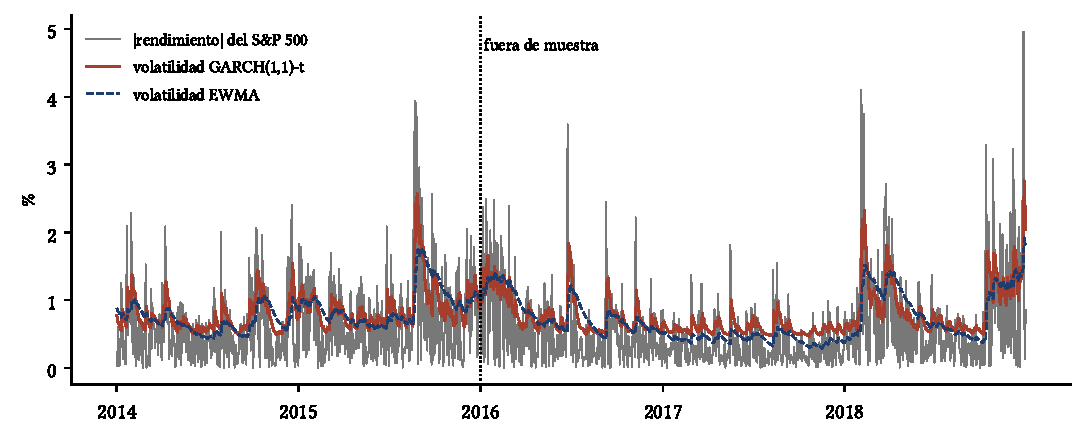
\includegraphics[width=\linewidth]{graficos/cap21_ej03_volatilidad.pdf}
\caption{Valor absoluto del rendimiento diario del S\&P 500 con las volatilidades GARCH(1,1)-$t$ y EWMA. A la derecha de la línea punteada, los parámetros del
GARCH están fijos en los estimados con 2014--2015.}
\label{fig:volatilidad21}
\end{figure}

\begin{conclusion}
Para pronosticar la volatilidad diaria, cualquier modelo dinámico es mucho mejor que uno constante, y la elección entre GARCH y EWMA es secundaria. Con
muestras cortas, la simplicidad de EWMA es una ventaja.
\end{conclusion}
\end{ejresuelto}

\begin{ejresuelto}{Etapa 4: VaR y ES de la cartera}\label{ej:etapa4}
\enunciado Para la cartera 1/N, calcule el VaR y el ES diarios al 99 y al 97,5\,\% de 2016 a 2018 con simulación histórica (250 días), EWMA normal y
GARCH(1,1)-$t$ (estimado en 2014--2015 y reestimado cada enero con todos los datos anteriores). Evalúe con las pruebas de Kupiec y de Christoffersen, y
compare la pérdida media en los días de excepción con el ES pronosticado.

\solucion
\paso{Paso 1. Resultados al 99\,\%} (754 días; 7,5 excepciones esperadas).
\begin{center}\small
\begin{tabular}{@{}lrrrr@{}}
\toprule
Método & Excepciones & $p$ Kupiec & $p$ Christoffersen & Pérdida/ES \\
\midrule
Simulación histórica & 14 & 0,035 & 0,466 & 1,043 \\
EWMA normal & 21 & 0,000 & 0,611 & 1,173 \\
GARCH-$t$ (fijo) & 14 & 0,035 & 0,466 & 0,931 \\
GARCH-$t$ (reestimado) & 13 & 0,070 & 0,499 & 0,931 \\
\bottomrule
\end{tabular}
\end{center}
El EWMA normal falla con claridad: 21 excepciones, casi el triple de las esperadas, porque la normal no tiene colas suficientes. Los demás también
subestiman el riesgo, pero menos. Solo el GARCH-$t$ reestimado cada año no se rechaza al 5\,\% (13 excepciones, $p=0{,}070$). Ninguno muestra excepciones
agrupadas.

\paso{Paso 2. Al 97,5\,\%} (18,9 esperadas): las cuatro alternativas tienen entre 27 y 28 excepciones. Los dos GARCH-$t$ no se rechazan ($p=0{,}074$); la
simulación histórica falla además la prueba de independencia ($p=0{,}019$), porque reacciona tarde a los cambios de volatilidad.

\paso{Paso 3. El ES.} En los días de excepción al 99\,\%, la pérdida realizada fue en promedio 0,93 veces el ES del GARCH-$t$: el ES fue suficiente. Con EWMA
normal fue 1,17 veces: el ES normal también es corto. Al reestimar con toda la muestra ($\alpha=0{,}141$, $\beta=0{,}831$, $\nu=4{,}34$), el pronóstico para el
primer día hábil de 2019, después de un diciembre de 2018 muy volátil, es una volatilidad de 2,87\,\%, un VaR al 99\,\% de 7,42\,\% y un ES de 10,18\,\%
(Figura~\ref{fig:var21}).

\codigoweb{cap21_ej04}
\salidaR{cap21_ej04_R.txt}
\lectura{cap21_ej04}

\RvsPy La reestimación anual usa en cada enero solo los datos de los años anteriores y filtra la varianza del año con esos parámetros. En R los
parámetros de cada día se guardan en una matriz indexada por fecha; en Python, en un diccionario. La simulación histórica del día $t$ usa las pérdidas
de $t-250$ a $t-1$.

\begin{figure}[ht]
\centering
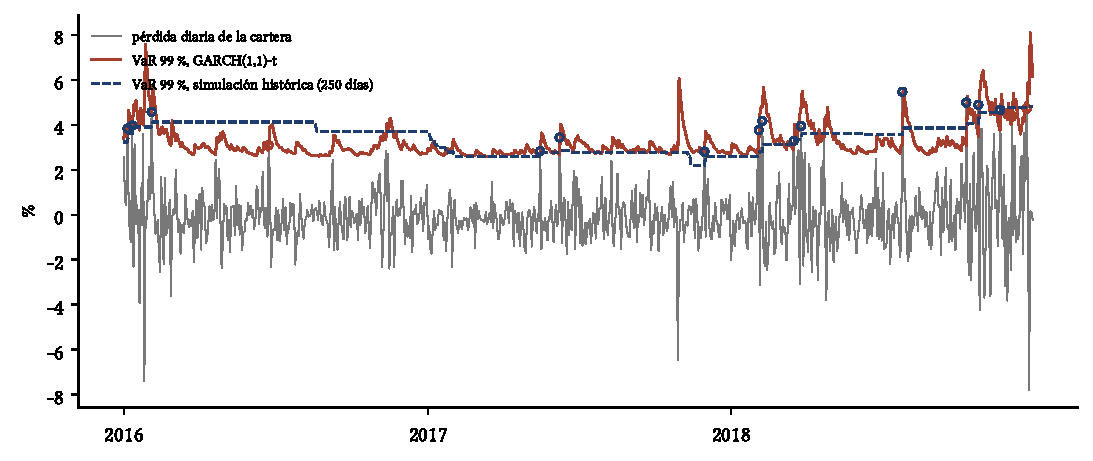
\includegraphics[width=\linewidth]{graficos/cap21_ej04_var.pdf}
\caption{Pérdida diaria de la cartera 1/N con el VaR al 99\,\% del GARCH(1,1)-$t$ fijo y de la simulación histórica, y sus excepciones (círculos).}
\label{fig:var21}
\end{figure}

\begin{conclusion}
Las colas pesadas importan más que la dinámica: la normal falla aunque su volatilidad sea dinámica. La recomendación al comité es un GARCH con errores $t$,
reestimado al menos una vez al año y con su prueba retrospectiva informada junto con la cifra de VaR.
\end{conclusion}
\end{ejresuelto}

\begin{ejresuelto}{Etapa 5: asignación fuera de muestra}\label{ej:etapa5}
\enunciado Desde enero de 2015, cada 21 días hábiles, forme la cartera 1/N y la de mínima varianza global con la covarianza muestral de los últimos 250 días y
con la covarianza EWMA. Compare media, volatilidad, razón de Sharpe, máxima caída y rotación.

\solucion
\paso{Paso 1. Resultados} (1\,007 días; 48 rebalanceos).
\begin{center}\small
\begin{tabular}{@{}lrrrrr@{}}
\toprule
Estrategia & Media (\%) & Vol.\ (\%) & Sharpe & Máx.\ caída (\%) & Rotación \\
\midrule
1/N & 23,42 & 21,82 & 1,073 & 29,52 & 0,000 \\
Mínima varianza (muestral) & 17,83 & 21,63 & 0,824 & 30,13 & 0,146 \\
Mínima varianza (EWMA) & 18,41 & 22,86 & 0,805 & 36,04 & 0,990 \\
\bottomrule
\end{tabular}
\end{center}
La cartera de mínima varianza con covarianza muestral reduce la volatilidad apenas de 21,82 a 21,63\,\% anual, y con covarianza EWMA la \emph{aumenta}. El
objetivo de la estrategia, reducir el riesgo, prácticamente no se logra: con cuatro activos de correlaciones parecidas, la cartera 1/N ya está cerca de la de
mínima varianza, y el error de estimación de $\Sigma$ consume la pequeña ganancia teórica. La versión EWMA rota casi el 100\,\% de la cartera en cada
rebalanceo, y su peso mínimo es negativo en promedio ($-0{,}096$).

\paso{Paso 2. ¿Es mejor 1/N?} Su razón de Sharpe es mayor, pero por la Proposición~\ref{prop:sesharpe}, con 1\,007 días,
\begin{align*}
  \text{ee}(\widehat{SR}_{\text{anual}}) &\approx \sqrt{252}\sqrt{\frac{1+(1{,}073/\sqrt{252})^2/2}{1\,007}}\\
                                         &= 0{,}501,
\end{align*}
de modo que las tres razones de Sharpe están a menos de un error estándar entre sí. Las dos estrategias principales tienen una correlación diaria de 0,95: son
casi la misma cartera. La mínima varianza muestral pondera más a Apple (0,41) y Alphabet (0,40), las de menor volatilidad, y menos a Amazon (0,06)
(Figura~\ref{fig:asignacion}).

\codigoweb{cap21_ej05}
\salidaR{cap21_ej05_R.txt}
\lectura{cap21_ej05}

\RvsPy Los pesos se calculan con \texttt{solve(S, 1)} en ambos lenguajes en lugar de invertir $\Sigma$. Se suponen pesos constantes entre rebalanceos (rebalanceo
diario implícito) y sin costos de transacción; con costos, la ventaja de 1/N, que nunca rota, sería mayor.

\begin{figure}[ht]
\centering
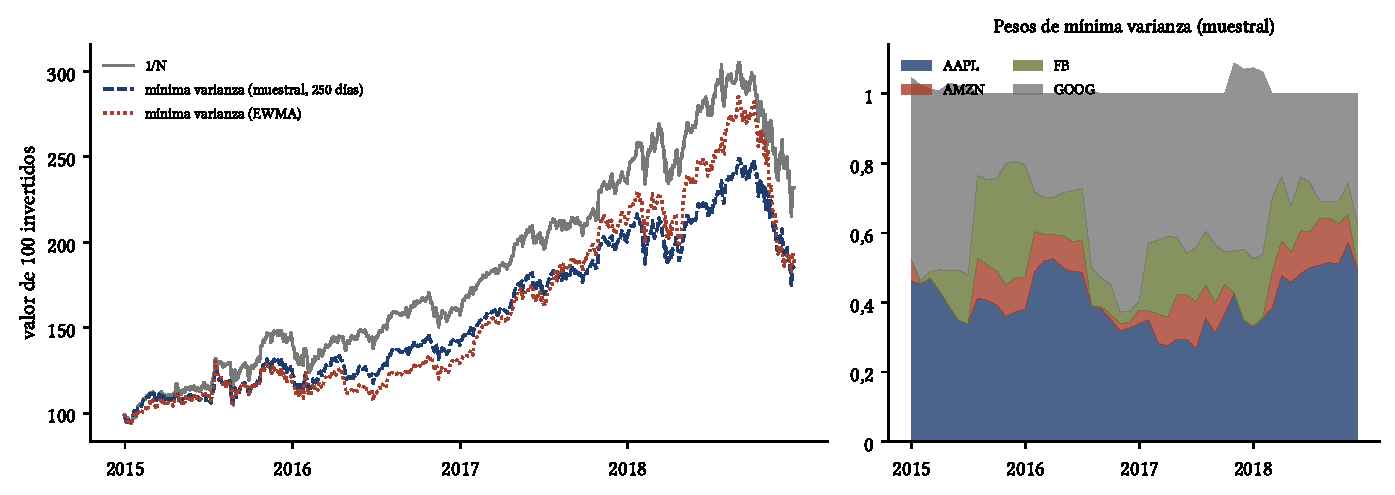
\includegraphics[width=\linewidth]{graficos/cap21_ej05_asignacion.pdf}
\caption{Izquierda: valor de 100 invertidos en cada estrategia desde enero de 2015. Derecha: pesos de la cartera de mínima varianza muestral en cada rebalanceo
(las posiciones cortas, en 12 de los 48 rebalanceos, se muestran como cero).}
\label{fig:asignacion}
\end{figure}

\begin{conclusion}
Optimizar no siempre mejora. Con pocos activos parecidos, la regla 1/N es tan buena como la de mínima varianza y no tiene costos de estimación ni de rotación,
como encontraron DeMiguel, Garlappi y Uppal (2009).
\end{conclusion}
\end{ejresuelto}

% ---------------------------------------------------------------------
\section{El informe al comité}
% ---------------------------------------------------------------------

Un informe útil responde cada pregunta en una o dos oraciones, con la cifra, su incertidumbre y la limitación principal:
\begin{enumerate}[label=\arabic*.,leftmargin=*]
  \item \textbf{Rendimientos.} Tienen colas mucho más pesadas que la normal (curtosis de 6,7 a 18,2) y volatilidad que se agrupa. Sus medias de 2014--2018
        reflejan la selección de ganadores y no deben extrapolarse.
  \item \textbf{Riesgo de mercado.} La cartera tiene una beta de 1,23 con el S\&P 500: amplifica el mercado. El alfa estimado no es evidencia de habilidad
        ni de rendimiento futuro.
  \item \textbf{Volatilidad.} Un modelo dinámico (GARCH o EWMA) es indispensable; entre ellos la diferencia no es significativa.
  \item \textbf{Pérdida máxima probable.} El VaR diario al 99\,\% para el primer día de 2019 es 7,4\,\% del valor de la cartera, y la pérdida media en el peor
        1\,\% de los días, 10,2\,\%. El modelo que lo calcula (GARCH-$t$ reestimado anualmente) pasó la prueba retrospectiva de 2016--2018 al 5\,\%, pero con
        13 excepciones frente a 7,5 esperadas: las cifras deben leerse como un mínimo.
  \item \textbf{Asignación.} Ponderar por igual es tan bueno como minimizar la varianza y más barato de mantener.
\end{enumerate}
Las limitaciones generales son tres: cinco años de datos de un período alcista, cuatro activos del mismo sector y la ausencia de costos de transacción.

% ---------------------------------------------------------------------
\section{Proyectos propuestos}
% ---------------------------------------------------------------------

\begin{enumerate}[label=\textbf{\thechapter.\arabic*},leftmargin=*,itemsep=6pt]
  \item \emph{(Cartera peruana.)} Repita el proyecto con cinco acciones de la BVL de distintos sectores (por ejemplo, minería, banca, consumo, construcción y
  energía) y el índice S\&P/BVL Perú General. ¿Cambia la conclusión sobre 1/N cuando las correlaciones son más bajas? Discuta el efecto de la negociación poco
  frecuente sobre las betas.

  \item \emph{(Sesgo de selección.)} Con los 30 carteras de French del Capítulo~\ref{cap:factores}, elija en cada enero las cuatro de mayor rendimiento en los 5 años
  anteriores y mida su rendimiento en el año siguiente. Compare con el alfa de la Etapa 2.

  \item \emph{(Cópulas.)} Sustituya en la Etapa 4 el GARCH univariado de la cartera por GARCH-$t$ marginales unidos por una cópula $t$ (Capítulo~\ref{cap:copulas}).
  ¿Mejora la prueba retrospectiva?

  \item \emph{(Regímenes.)} Estime un modelo de dos regímenes (Capítulo~\ref{cap:markov}) para los rendimientos semanales de la cartera y úselo para el VaR semanal.

  \item \emph{(Costos.)} Agregue a la Etapa 5 un costo de 10 puntos básicos por unidad de rotación. ¿Cuánto cambia la razón de Sharpe de cada estrategia?

  \item \emph{(Contracción.)} Sustituya la covarianza muestral de la Etapa 5 por la de Ledoit y Wolf (2004), que contrae hacia una matriz con correlación constante.

  \item \emph{(Evaluación del ES.)} Implemente la prueba de Acerbi y Szekely (2014) para el ES de la Etapa 4.

  \item \emph{(Informe.)} Redacte el informe al comité en no más de dos páginas, con una tabla y una figura, para un lector sin formación econométrica.
\end{enumerate}

% ---------------------------------------------------------------------
\section{Resumen de fórmulas}
% ---------------------------------------------------------------------

\begin{table}[H]
\centering\small
\begin{tabular}{@{}ll@{}}
\toprule
Concepto & Fórmula \\
\midrule
Mínima varianza global & $\mathbf w^*=\Sigma^{-1}\mathbf 1/(\mathbf 1'\Sigma^{-1}\mathbf 1)$;\quad $\sigma^2_{\min}=1/(\mathbf 1'\Sigma^{-1}\mathbf 1)$ \\
Error estándar del Sharpe & $\sqrt{(1+SR^2/2)/T}$ \\
Pruebas múltiples & $\Pr(\ge1\text{ rechazo})=1-(1-\alpha)^K$;\quad Bonferroni $\alpha/K$ \\
QLIKE & $\ln h_t+e_t^2/h_t$ \\
Vida media de la volatilidad & $\ln0{,}5/\ln(\alpha+\beta)$ \\
Rotación & $\sum_j|w_{j,k}-w_{j,k-1}|$ \\
Máxima caída & $1-\min_t V_t/\max_{s\le t}V_s$ \\
\bottomrule
\end{tabular}
\caption{Fórmulas principales del Capítulo 21.}
\end{table}

\section*{Referencias}
\begin{itemize}[leftmargin=*]
  \item Acerbi, C. y Szekely, B. (2014). Backtesting expected shortfall. \emph{Risk}, 27(11), 76--81.
  \item DeMiguel, V., Garlappi, L. y Uppal, R. (2009). Optimal versus naive diversification: How inefficient is the 1/N portfolio strategy?
        \emph{Review of Financial Studies}, 22(5), 1915--1953.
  \item Harvey, C. R., Liu, Y. y Zhu, H. (2016). \ldots\ and the cross-section of expected returns. \emph{Review of Financial Studies}, 29(1), 5--68.
  \item Ledoit, O. y Wolf, M. (2004). Honey, I shrunk the sample covariance matrix. \emph{Journal of Portfolio Management}, 30(4), 110--119.
  \item Lo, A. W. (2002). The statistics of Sharpe ratios. \emph{Financial Analysts Journal}, 58(4), 36--52.
  \item Merton, R. C. (1980). On estimating the expected return on the market: An exploratory investigation. \emph{Journal of Financial Economics},
        8(4), 323--361.
  \item Patton, A. J. (2011). Volatility forecast comparison using imperfect volatility proxies. \emph{Journal of Econometrics}, 160(1), 246--256.
\end{itemize}

% =====================================================================
%  Apéndices — Econometría Financiera Aplicada (Jeel Cueva)
% =====================================================================
\appendix

% =====================================================================
\chapter{Herramientas de probabilidad y estadística}\label{ap:prob}
% =====================================================================

Este apéndice reúne los resultados de probabilidad que el libro usa sin demostrar en el texto
principal. Se presentan con la notación de los capítulos: $X,Y$ son variables aleatorias, $\E$ es la
esperanza, $\Var$ la varianza y $\Cov$ la covarianza.

\section{Esperanza, varianza y covarianza}

\begin{proposicion}\label{prop:ap-var}
Para constantes $a,b$ y variables con segundo momento finito,
\[
  \Var(aX+bY)=a^2\Var(X)+b^2\Var(Y)+2ab\Cov(X,Y).
\]
En forma matricial, si $\bm X$ es un vector aleatorio con matriz de covarianzas $\bm\Sigma$ y $\bm w$ un
vector de constantes, $\Var(\bm w'\bm X)=\bm w'\bm\Sigma\bm w$.
\end{proposicion}

\begin{proof}
Sea $\mu_X=\E X$ y $\mu_Y=\E Y$. Por la linealidad de la esperanza:
\begin{align*}
  \Var(aX+bY) &= \E\bigl[(aX+bY-a\mu_X-b\mu_Y)^2\bigr]\\
              &= \E\bigl[(a(X-\mu_X)+b(Y-\mu_Y))^2\bigr]\\
              &= a^2\E\bigl[(X-\mu_X)^2\bigr]+b^2\E\bigl[(Y-\mu_Y)^2\bigr]+2ab\,\E\bigl[(X-\mu_X)(Y-\mu_Y)\bigr]\\
              &= a^2\Var(X)+b^2\Var(Y)+2ab\Cov(X,Y).
\end{align*}
Para la forma matricial, con $\bm\mu=\E\bm X$:
\begin{align*}
  \Var(\bm w'\bm X) &= \E\bigl[(\bm w'\bm X-\bm w'\bm\mu)^2\bigr]\\
                    &= \E\bigl[\bm w'(\bm X-\bm\mu)(\bm X-\bm\mu)'\bm w\bigr]\\
                    &= \bm w'\,\E\bigl[(\bm X-\bm\mu)(\bm X-\bm\mu)'\bigr]\,\bm w\\
                    &= \bm w'\bm\Sigma\bm w. \qedhere
\end{align*}
\end{proof}

La segunda forma es la varianza de un portafolio con pesos $\bm w$ (Capítulos~3 y~12). Como una varianza
no puede ser negativa, $\bm w'\bm\Sigma\bm w\ge0$ para todo $\bm w$: toda matriz de covarianzas es
semidefinida positiva.

\begin{proposicion}[Esperanza iterada]\label{prop:ap-iterada}
Si $\E|X|<\infty$, entonces $\E[X]=\E\bigl[\E(X\mid Y)\bigr]$. En particular, si $\E(u_t\mid
\mathcal F_{t-1})=0$, entonces $\E u_t=0$ y $\Cov(u_t,Z)=0$ para toda $Z$ medible respecto de
$\mathcal F_{t-1}$ con segundo momento finito.
\end{proposicion}

\begin{proof}
La primera parte es la propiedad de la torre de la esperanza condicional. Para la segunda:
\begin{align*}
  \E u_t     &= \E\bigl[\E(u_t\mid\mathcal F_{t-1})\bigr]=\E[0]=0,\\
  \Cov(u_t,Z)&= \E[u_tZ]-\E u_t\,\E Z\\
             &= \E\bigl[\E(u_tZ\mid\mathcal F_{t-1})\bigr]\\
             &= \E\bigl[Z\,\E(u_t\mid\mathcal F_{t-1})\bigr]\\
             &= 0. \qedhere
\end{align*}
\end{proof}

Este resultado justifica que las innovaciones de un modelo GARCH (Capítulo~8) o de un modelo de
expectativas racionales no estén correlacionadas con ninguna información pasada.

\section{Distribuciones derivadas de la normal}

\begin{definicion}
Sean $Z_1,\dots,Z_k$ independientes $N(0,1)$ y $V\sim\chi^2_m$, $W\sim\chi^2_n$ independientes entre sí.
\begin{enumerate}[label=(\roman*)]
  \item $Q=\sum_{i=1}^kZ_i^2$ tiene distribución \emph{chi-cuadrado} con $k$ grados de libertad, $\chi^2_k$.
  \item $t=Z_1/\sqrt{V/m}$, con $Z_1$ independiente de $V$, tiene distribución \emph{$t$ de Student} con $m$
        grados de libertad, $t_m$.
  \item $F=(V/m)/(W/n)$ tiene distribución \emph{$F$ de Snedecor} con $(m,n)$ grados de libertad, $F_{m,n}$.
\end{enumerate}
\end{definicion}

\begin{proposicion}\label{prop:ap-chi}
Si $Q\sim\chi^2_k$, entonces $\E Q=k$ y $\Var Q=2k$.
\end{proposicion}

\begin{proof}
Para $Z\sim N(0,1)$ se cumple $\E Z^2=1$ y $\E Z^4=3$. Entonces:
\begin{align*}
  \E Q          &= \sum_{i=1}^k\E Z_i^2\\
                &= k,\\
  \Var(Z_i^2)   &= \E Z_i^4-(\E Z_i^2)^2\\
                &= 3-1\\
                &= 2,\\
  \Var Q        &= \sum_{i=1}^k\Var(Z_i^2) && \text{(independencia)}\\
                &= 2k. \qedhere
\end{align*}
\end{proof}

Las tres distribuciones se usan en todo el libro: la $\chi^2$ en las pruebas de Wald, de razón de
verosimilitud y de Jarque-Bera; la $t$ en las pruebas sobre un coeficiente y como distribución de las
innovaciones GARCH; la $F$ en las pruebas de restricciones lineales y en la prueba GRS. La
Figura~\ref{fig:apdist} muestra sus densidades. La $t$ tiene colas más pesadas que la normal (con $m=1$
es la distribución de Cauchy, sin media) y converge a la $N(0,1)$ cuando $m\to\infty$; la $\chi^2_k$
es asimétrica a la derecha y se vuelve más simétrica al crecer $k$; y $mF_{m,n}$ converge a $\chi^2_m$
cuando $n\to\infty$.

\begin{figure}[H]
\centering
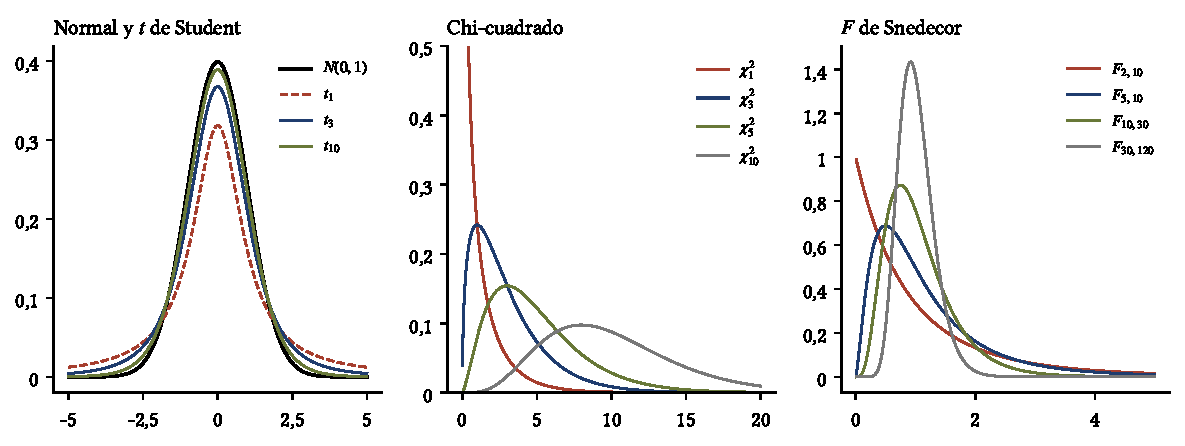
\includegraphics[width=\linewidth]{graficos/apA_fig_distribuciones.pdf}
\caption{Densidades de la normal estándar y de la $t$ de Student (izquierda), de la chi-cuadrado
(centro) y de la $F$ de Snedecor (derecha) para distintos grados de libertad.}
\label{fig:apdist}
\end{figure}

\section{Convergencia y teoremas límite}

\begin{definicion}
Una sucesión $X_T$ \emph{converge en probabilidad} a $c$, $X_T\xrightarrow{p}c$, si para todo
$\varepsilon>0$, $\Pr(|X_T-c|>\varepsilon)\to0$. Converge \emph{en distribución} a $X$,
$X_T\xrightarrow{d}X$, si $\Pr(X_T\le x)\to\Pr(X\le x)$ en todo punto de continuidad de la función de
distribución de $X$.
\end{definicion}

\begin{teorema}[Ley débil de los grandes números]\label{teo:ap-lgn}
Si $X_1,\dots,X_T$ no están correlacionadas, tienen media $\mu$ y varianza $\sigma^2<\infty$, entonces
$\bar X_T\xrightarrow{p}\mu$.
\end{teorema}

\begin{proof}
Por la desigualdad de Chebyshev y la Proposición~\ref{prop:ap-var} (con covarianzas nulas):
\begin{align*}
  \Pr\bigl(|\bar X_T-\mu|>\varepsilon\bigr) &\le \frac{\Var(\bar X_T)}{\varepsilon^2}\\
                                           &= \frac{1}{\varepsilon^2}\cdot\frac{1}{T^2}\sum_{t=1}^T\Var(X_t)\\
                                           &= \frac{\sigma^2}{T\varepsilon^2}\\
                                           &\longrightarrow 0. \qedhere
\end{align*}
\end{proof}

\begin{teorema}[Teorema central del límite de Lindeberg-Lévy]\label{teo:ap-tcl}
Si $X_1,\dots,X_T$ son independientes e idénticamente distribuidas con media $\mu$ y varianza
$\sigma^2\in(0,\infty)$, entonces
\[
  \sqrt T\,\frac{\bar X_T-\mu}{\sigma}\xrightarrow{d}N(0,1).
\]
\end{teorema}

La demostración usa funciones características y puede consultarse en cualquier texto de probabilidad.
Para series temporales existen versiones para diferencias de martingala y para procesos con dependencia
débil (Capítulos~4 y~6), que son las que justifican los errores estándar robustos. La
Figura~\ref{fig:aptcl} ilustra el teorema con una distribución muy asimétrica: la exponencial.

\begin{figure}[H]
\centering
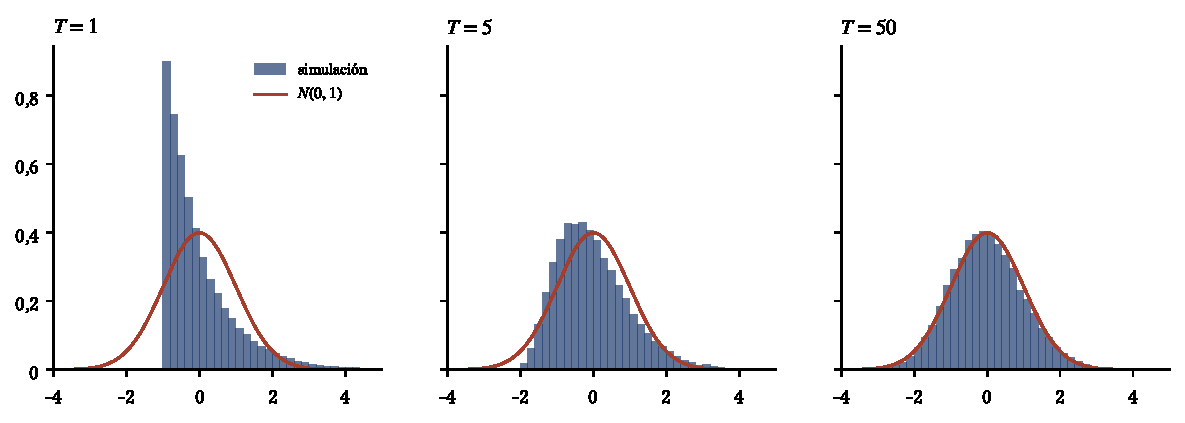
\includegraphics[width=\linewidth]{graficos/apA_fig_tcl.pdf}
\caption{Teorema central del límite: distribución de $\sqrt T(\bar X_T-1)$ con $X_t$ exponenciales de
media y desviación estándar 1, en 50\,000 simulaciones (semilla 2026), para $T=1$, 5 y 50.}
\label{fig:aptcl}
\end{figure}

\begin{teorema}[Slutsky]\label{teo:ap-slutsky}
Si $X_T\xrightarrow{d}X$ y $Y_T\xrightarrow{p}c$, con $c$ constante, entonces $X_T+Y_T\xrightarrow{d}X+c$,
$X_TY_T\xrightarrow{d}cX$ y, si $c\ne0$, $X_T/Y_T\xrightarrow{d}X/c$.
\end{teorema}

Por el teorema de Slutsky, se puede reemplazar $\sigma$ por un estimador consistente $\hat\sigma$ en el
TCL sin cambiar la distribución límite: así se obtienen los estadísticos $t$ asintóticos.

\begin{teorema}[Método delta]\label{teo:ap-delta}
Si $\sqrt T(\hat{\bm\theta}-\bm\theta)\xrightarrow{d}N(\bm0,\bm V)$ y $g$ es una función con gradiente
$\nabla g(\bm\theta)\ne\bm0$ continuo en $\bm\theta$, entonces
\[
  \sqrt T\bigl(g(\hat{\bm\theta})-g(\bm\theta)\bigr)\xrightarrow{d}
  N\bigl(0,\ \nabla g(\bm\theta)'\,\bm V\,\nabla g(\bm\theta)\bigr).
\]
\end{teorema}

\begin{proof}[Idea de la demostración]
Por el teorema del valor medio, existe $\bar{\bm\theta}$ entre $\hat{\bm\theta}$ y $\bm\theta$ tal que
\begin{align*}
  g(\hat{\bm\theta})                     &= g(\bm\theta)+\nabla g(\bar{\bm\theta})'(\hat{\bm\theta}-\bm\theta),\\
  \sqrt T\bigl(g(\hat{\bm\theta})-g(\bm\theta)\bigr) &= \nabla g(\bar{\bm\theta})'\,\sqrt T(\hat{\bm\theta}-\bm\theta).
\end{align*}
Como $\hat{\bm\theta}\xrightarrow{p}\bm\theta$, también $\bar{\bm\theta}\xrightarrow{p}\bm\theta$ y, por la
continuidad del gradiente, $\nabla g(\bar{\bm\theta})\xrightarrow{p}\nabla g(\bm\theta)$. Por el teorema de
Slutsky, el lado derecho converge a $\nabla g(\bm\theta)'\bm Y$ con $\bm Y\sim N(\bm0,\bm V)$, cuya
varianza es $\nabla g(\bm\theta)'\bm V\nabla g(\bm\theta)$ (Proposición~\ref{prop:ap-var}).
\end{proof}

\section{Ejercicio resuelto}

\begin{ejresuelto}{Precisión de la razón media/desviación de \texttt{EPU} y del S\&P 500}\label{ej:apdelta}
\enunciado Sea $\theta=\mu/\sigma$ la razón entre la media y la desviación estándar del rendimiento
mensual (la razón de Sharpe cuando la tasa libre de riesgo es cero). (a) Con el método delta, obtenga la
varianza asintótica de $\hat\theta=\hat\mu/\hat\sigma$ para rendimientos independientes con asimetría
$\gamma_3$ y curtosis $\gamma_4$, y su caso normal. (b) Calcule $\hat\theta$, su error estándar y un
intervalo de confianza del 95\,\% para \texttt{EPU} y el S\&P 500, con datos mensuales de 2015--2025.

\solucion
\paso{Paso 1. Distribución conjunta de $(\hat\mu,\hat\sigma^2)$.} Con $\mu_j=\E(R-\mu)^j$, se cumple
\begin{align*}
  \Var(\hat\mu)          &\approx \frac{\sigma^2}{T},\\
  \Cov(\hat\mu,\hat\sigma^2) &\approx \frac{\mu_3}{T},\\
  \Var(\hat\sigma^2)     &\approx \frac{\mu_4-\sigma^4}{T}.
\end{align*}
\paso{Paso 2. Gradiente.} Con $g(a,b)=a/\sqrt b$, evaluado en $(\mu,\sigma^2)$:
\begin{align*}
  \frac{\partial g}{\partial a} &= \frac{1}{\sqrt b}=\frac1\sigma,\\
  \frac{\partial g}{\partial b} &= -\frac{a}{2b^{3/2}}=-\frac{\mu}{2\sigma^3}.
\end{align*}
\paso{Paso 3. Método delta.} Por el Teorema~\ref{teo:ap-delta}, $T\Var(\hat\theta)\approx v$ con
\begin{align*}
  v &= \frac{1}{\sigma^2}\sigma^2+2\cdot\frac1\sigma\cdot\Bigl(-\frac{\mu}{2\sigma^3}\Bigr)\mu_3
       +\frac{\mu^2}{4\sigma^6}\bigl(\mu_4-\sigma^4\bigr)\\
    &= 1-\frac{\mu}{\sigma}\cdot\frac{\mu_3}{\sigma^3}+\frac{\mu^2}{4\sigma^2}\Bigl(\frac{\mu_4}{\sigma^4}-1\Bigr)\\
    &= 1-\theta\gamma_3+\frac{\theta^2}{4}(\gamma_4-1).
\end{align*}
Bajo normalidad, $\gamma_3=0$ y $\gamma_4=3$, de modo que
\begin{align*}
  v &= 1+\frac{\theta^2}{4}(3-1)\\
    &= 1+\frac{\theta^2}{2}.
\end{align*}
\paso{Paso 4. Cálculo.}

\codigoweb{apA_ej01}
\salidaR{apA_ej01_R.txt}
\lectura{apA_ej01}

\RvsPy Ambos programas calculan los momentos con divisor $T$, tal como aparecen en el Paso~1, y dan
las mismas cifras.

\begin{conclusion}
Con 132 meses, el error estándar de $\hat\theta$ es cercano a $1/\sqrt{132}\approx0{,}087$ en ambas
series. Esa precisión es baja: el intervalo del 95\,\% para \texttt{EPU} incluye el cero, así que once años
de datos no bastan para afirmar que su rendimiento medio fue positivo. El del S\&P 500 lo excluye por
poco. La corrección por asimetría negativa y curtosis aumenta el error estándar entre 2\,\% y 5\,\%.
\end{conclusion}
\end{ejresuelto}

\section{Ejercicios propuestos}

\begin{enumerate}[label=\textbf{A.\arabic*},leftmargin=*,itemsep=6pt]
  \item Demuestre que si $X\sim N(\mu,\sigma^2)$, entonces $\E e^{X}=e^{\mu+\sigma^2/2}$, y úselo para
        obtener la media de un precio lognormal (Capítulo~1).
  \item Demuestre que si $t\sim t_m$ con $m>2$, entonces $\Var(t)=m/(m-2)$, y explique por qué el
        Capítulo~8 reescala las innovaciones $t$ para que tengan varianza unitaria.
  \item Use el método delta para obtener el error estándar de la volatilidad anualizada
        $\hat\sigma\sqrt{252}$ a partir de $\Var(\hat\sigma^2)\approx(\mu_4-\sigma^4)/T$. Aplíquelo a los
        rendimientos diarios de \texttt{BVN} del Ejercicio~\ref{ej:anualizar}.
  \item \emph{(Simulación.)} Repita la Figura~\ref{fig:aptcl} con rendimientos $t_3$ en lugar de
        exponenciales. ¿Converge más rápido o más lento? ¿Y con $t_2$, que no tiene varianza finita?
\end{enumerate}

% =====================================================================
\chapter{Álgebra matricial para econometría}\label{ap:matrices}
% =====================================================================

\section{Definiciones básicas}

Una matriz cuadrada $\bm A$ es \emph{simétrica} si $\bm A=\bm A'$, \emph{idempotente} si $\bm A\bm A=\bm A$
y \emph{definida positiva} si $\bm x'\bm A\bm x>0$ para todo $\bm x\ne\bm0$ (semidefinida positiva si
$\ge0$). La \emph{traza} es la suma de la diagonal, $\operatorname{tr}\bm A=\sum_ia_{ii}$, y cumple
$\operatorname{tr}(\bm A\bm B)=\operatorname{tr}(\bm B\bm A)$ siempre que ambos productos existan. El
\emph{rango} de $\bm X$ ($T\times k$) es el número de columnas linealmente independientes; si
$\operatorname{rango}\bm X=k$, la matriz $\bm X'\bm X$ es definida positiva y, por tanto, invertible.

\begin{proposicion}\label{prop:ap-xx}
Si $\operatorname{rango}\bm X=k$, entonces $\bm X'\bm X$ es definida positiva.
\end{proposicion}

\begin{proof}
Sea $\bm c\ne\bm0$ y $\bm v=\bm X\bm c$. Como las columnas de $\bm X$ son linealmente independientes,
$\bm v\ne\bm0$. Entonces
\begin{align*}
  \bm c'\bm X'\bm X\bm c &= (\bm X\bm c)'(\bm X\bm c)\\
                         &= \bm v'\bm v\\
                         &= \sum_{t=1}^Tv_t^2\\
                         &> 0. \qedhere
\end{align*}
\end{proof}

\section{Derivadas de formas lineales y cuadráticas}

\begin{proposicion}\label{prop:ap-deriv}
Sean $\bm a$ y $\bm x$ vectores $k\times1$ y $\bm A$ una matriz $k\times k$. Entonces
\[
  \frac{\partial\,\bm a'\bm x}{\partial\bm x}=\bm a,\qquad
  \frac{\partial\,\bm x'\bm A\bm x}{\partial\bm x}=(\bm A+\bm A')\bm x,
\]
que es igual a $2\bm A\bm x$ cuando $\bm A$ es simétrica.
\end{proposicion}

\begin{proof}
Para la forma lineal, $\bm a'\bm x=\sum_ia_ix_i$, y su derivada respecto de $x_j$ es $a_j$. Para la
forma cuadrática:
\begin{align*}
  \bm x'\bm A\bm x &= \sum_{i=1}^k\sum_{l=1}^k a_{il}x_ix_l,\\
  \frac{\partial\,\bm x'\bm A\bm x}{\partial x_j} &= \sum_{l=1}^ka_{jl}x_l+\sum_{i=1}^ka_{ij}x_i\\
                                                   &= (\bm A\bm x)_j+(\bm A'\bm x)_j .
\end{align*}
Apilando las $k$ derivadas se obtiene $(\bm A+\bm A')\bm x$.
\end{proof}

\section{Mínimos cuadrados en forma matricial}

\begin{proposicion}\label{prop:ap-mco}
Sea $\bm y=\bm X\bm\beta+\bm u$, con $\bm X$ de rango $k$. El vector que minimiza
$S(\bm b)=(\bm y-\bm X\bm b)'(\bm y-\bm X\bm b)$ es $\hat{\bm\beta}=(\bm X'\bm X)^{-1}\bm X'\bm y$.
\end{proposicion}

\begin{proof}
Expandimos la suma de cuadrados y derivamos con la Proposición~\ref{prop:ap-deriv}:
\begin{align*}
  S(\bm b) &= \bm y'\bm y-\bm b'\bm X'\bm y-\bm y'\bm X\bm b+\bm b'\bm X'\bm X\bm b\\
           &= \bm y'\bm y-2\bm y'\bm X\bm b+\bm b'\bm X'\bm X\bm b,\\
  \frac{\partial S}{\partial\bm b} &= -2\bm X'\bm y+2\bm X'\bm X\bm b .
\end{align*}
Igualando a cero se obtienen las ecuaciones normales:
\begin{align*}
  \bm X'\bm X\hat{\bm\beta} &= \bm X'\bm y,\\
  \hat{\bm\beta}            &= (\bm X'\bm X)^{-1}\bm X'\bm y .
\end{align*}
La matriz de segundas derivadas es $2\bm X'\bm X$, definida positiva por la
Proposición~\ref{prop:ap-xx}, así que el punto crítico es el mínimo global.
\end{proof}

\begin{proposicion}[Matrices de proyección]\label{prop:ap-proy}
Sean $\bm P=\bm X(\bm X'\bm X)^{-1}\bm X'$ y $\bm M=\bm I-\bm P$. Entonces $\bm P$ y $\bm M$ son
simétricas e idempotentes, $\bm P\bm X=\bm X$, $\bm M\bm X=\bm0$, los valores ajustados son
$\hat{\bm y}=\bm P\bm y$, los residuos son $\hat{\bm u}=\bm M\bm y=\bm M\bm u$ y
$\operatorname{tr}\bm M=T-k$.
\end{proposicion}

\begin{proof}
La simetría es inmediata porque $(\bm X'\bm X)^{-1}$ es simétrica. Idempotencia y anulación:
\begin{align*}
  \bm P\bm P &= \bm X(\bm X'\bm X)^{-1}\bm X'\bm X(\bm X'\bm X)^{-1}\bm X'\\
             &= \bm X(\bm X'\bm X)^{-1}\bm X'\\
             &= \bm P,\\
  \bm P\bm X &= \bm X(\bm X'\bm X)^{-1}\bm X'\bm X\\
             &= \bm X,\\
  \bm M\bm X &= \bm X-\bm P\bm X\\
             &= \bm 0,\\
  \bm M\bm M &= \bm I-2\bm P+\bm P\bm P\\
             &= \bm M .
\end{align*}
Los residuos y la traza:
\begin{align*}
  \hat{\bm u} &= \bm y-\bm X\hat{\bm\beta}\\
              &= \bm y-\bm P\bm y\\
              &= \bm M\bm y\\
              &= \bm M(\bm X\bm\beta+\bm u)\\
              &= \bm M\bm u,\\
  \operatorname{tr}\bm P &= \operatorname{tr}\bigl((\bm X'\bm X)^{-1}\bm X'\bm X\bigr)\\
                         &= \operatorname{tr}\bm I_k\\
                         &= k,\\
  \operatorname{tr}\bm M &= T-k. \qedhere
\end{align*}
\end{proof}

La traza de $\bm M$ explica el divisor $T-k$ del estimador insesgado de la varianza del error: como
$\E(\hat{\bm u}'\hat{\bm u})=\E(\bm u'\bm M\bm u)=\sigma^2\operatorname{tr}\bm M=\sigma^2(T-k)$ cuando
$\E(\bm u\bm u'\mid\bm X)=\sigma^2\bm I$.

\section{El teorema de Frisch-Waugh-Lovell}

\begin{teorema}[Frisch-Waugh-Lovell]\label{teo:ap-fwl}
Particione $\bm X=[\bm X_1\ \bm X_2]$ y $\hat{\bm\beta}=(\hat{\bm\beta}_1',\hat{\bm\beta}_2')'$, y sea
$\bm M_1=\bm I-\bm X_1(\bm X_1'\bm X_1)^{-1}\bm X_1'$. Entonces
\[
  \hat{\bm\beta}_2=(\bm X_2'\bm M_1\bm X_2)^{-1}\bm X_2'\bm M_1\bm y,
\]
es decir, $\hat{\bm\beta}_2$ se obtiene regresando los residuos de $\bm y$ sobre $\bm X_1$ en los
residuos de $\bm X_2$ sobre $\bm X_1$.
\end{teorema}

\begin{proof}
Escribimos $\bm y=\bm X_1\hat{\bm\beta}_1+\bm X_2\hat{\bm\beta}_2+\hat{\bm u}$, donde $\hat{\bm u}$ es
ortogonal a $\bm X_1$ y a $\bm X_2$ por las ecuaciones normales. Premultiplicamos por $\bm M_1$, que anula
a $\bm X_1$ y deja intacto a $\hat{\bm u}$ (porque $\bm X_1'\hat{\bm u}=\bm0$):
\begin{align*}
  \bm M_1\bm y &= \bm M_1\bm X_1\hat{\bm\beta}_1+\bm M_1\bm X_2\hat{\bm\beta}_2+\bm M_1\hat{\bm u}\\
               &= \bm M_1\bm X_2\hat{\bm\beta}_2+\hat{\bm u}.
\end{align*}
Premultiplicamos por $\bm X_2'$ y usamos $\bm X_2'\hat{\bm u}=\bm0$:
\begin{align*}
  \bm X_2'\bm M_1\bm y &= \bm X_2'\bm M_1\bm X_2\hat{\bm\beta}_2+\bm X_2'\hat{\bm u}\\
                       &= \bm X_2'\bm M_1\bm X_2\hat{\bm\beta}_2,\\
  \hat{\bm\beta}_2     &= (\bm X_2'\bm M_1\bm X_2)^{-1}\bm X_2'\bm M_1\bm y . \qedhere
\end{align*}
\end{proof}

El teorema explica por qué incluir una constante equivale a trabajar con datos centrados, por qué los
efectos fijos del Capítulo~19 se estiman con datos en desviaciones respecto de la media de cada
individuo, y por qué el coeficiente de un factor en una regresión múltiple (Capítulo~14) mide su efecto
\emph{neto} de los demás factores.

\section{Producto de Kronecker y operador vec}

El producto de Kronecker de $\bm A$ ($m\times n$) y $\bm B$ ($p\times q$) es la matriz $mp\times nq$
\[
  \bm A\otimes\bm B=\begin{pmatrix}a_{11}\bm B&\cdots&a_{1n}\bm B\\ \vdots&\ddots&\vdots\\
                    a_{m1}\bm B&\cdots&a_{mn}\bm B\end{pmatrix},
\]
y $\operatorname{vec}\bm A$ apila las columnas de $\bm A$ en un vector $mn\times1$. Se usan para escribir
los modelos VAR (Capítulo~10) y los sistemas de ecuaciones de forma compacta.

\begin{proposicion}\label{prop:ap-vec}
Para matrices conformables, $\operatorname{vec}(\bm A\bm B\bm C)=(\bm C'\otimes\bm A)\operatorname{vec}\bm B$.
\end{proposicion}

\begin{proof}
Sea $\bm b_l$ la columna $l$ de $\bm B$ y $c_{lj}$ el elemento $(l,j)$ de $\bm C$. La columna $j$ de
$\bm A\bm B\bm C$ es
\begin{align*}
  (\bm A\bm B\bm C)_{\cdot j} &= \bm A\,(\bm B\bm C)_{\cdot j}\\
                              &= \bm A\sum_lc_{lj}\bm b_l\\
                              &= \sum_l c_{lj}\,\bm A\bm b_l\\
                              &= \bigl(c_{1j}\bm A\ \ c_{2j}\bm A\ \cdots\bigr)\operatorname{vec}\bm B .
\end{align*}
El bloque $(c_{1j}\bm A\ \ c_{2j}\bm A\ \cdots)$ es la fila de bloques $j$ de $\bm C'\otimes\bm A$, porque
el elemento $(j,l)$ de $\bm C'$ es $c_{lj}$. Apilando las columnas $j=1,2,\dots$ se obtiene el resultado.
\end{proof}

\section{Ejercicios propuestos}

\begin{enumerate}[label=\textbf{B.\arabic*},leftmargin=*,itemsep=6pt]
  \item Demuestre que $\operatorname{tr}(\bm A\bm B)=\operatorname{tr}(\bm B\bm A)$ y úselo para probar
        que $\E(\bm u'\bm M\bm u)=\sigma^2(T-k)$.
  \item Verifique numéricamente el Teorema~\ref{teo:ap-fwl} con los datos del Ejercicio~\ref{ej:portafolio}:
        regrese el rendimiento mensual de \texttt{BAP} sobre una constante, \texttt{SCCO} y \texttt{BVN},
        y compare el coeficiente de \texttt{BVN} con el de la regresión de residuos.
  \item Demuestre que los valores propios de una matriz idempotente son 0 o 1 y que su rango es igual a
        su traza.
  \item Demuestre que $(\bm A\otimes\bm B)(\bm C\otimes\bm D)=\bm A\bm C\otimes\bm B\bm D$ y que
        $(\bm A\otimes\bm B)^{-1}=\bm A^{-1}\otimes\bm B^{-1}$ cuando las inversas existen.
\end{enumerate}

% =====================================================================
\chapter{Datos, programas y reproducibilidad}\label{ap:datos}
% =====================================================================

\section{Organización del proyecto}

Todos los resultados numéricos del libro son la salida real de un programa. El proyecto se organiza
así:
\begin{itemize}[leftmargin=*]
  \item \texttt{capitulos/}: un archivo \texttt{.tex} por capítulo; \texttt{main.tex} los reúne.
  \item \texttt{datos/peru/} y \texttt{datos/internacional/}: series descargadas, en CSV, con un archivo
        \texttt{FUENTES.txt} que documenta el origen y la fecha de descarga de cada una.
  \item \texttt{codigo/R/} y \texttt{codigo/Python/}: un programa por ejercicio
        (\texttt{capNN\_ejMM.R} y \texttt{capNN\_ejMM.py}). Para que el libro no se haga extenso, los programas
        no se imprimen: están completos, con sus salidas en ambos lenguajes, en el repositorio del libro en GitHub (véase el Prefacio).
  \item \texttt{salidas/}: la salida de consola de cada programa; el libro inserta tal cual la salida en R.
  \item \texttt{graficos/}: figuras en PDF generadas por los programas de Python.
  \item \texttt{lecturas/}: las tablas ``Cómo leer la salida'' que siguen a cada salida de R. Su texto está
        en la subcarpeta \texttt{fuente/} y el programa \texttt{generar.py} las convierte en tablas.
\end{itemize}
Los programas se ejecutan desde la carpeta raíz del proyecto:
\begin{lstlisting}[style=salida,title={\small\sffamily\color{gray}Terminal}]
Rscript codigo/R/cap01_ej01.R > salidas/cap01_ej01_R.txt
PYTHONPATH=codigo/Python python3 codigo/Python/cap01_ej01.py > salidas/cap01_ej01_Py.txt
\end{lstlisting}
Se requiere R base (y el paquete \texttt{jsonlite} solo para descargar datos) y, en Python, \texttt{numpy},
\texttt{pandas}, \texttt{scipy}, \texttt{statsmodels} y \texttt{matplotlib}; \texttt{arch} y
\texttt{linearmodels} se usan para comprobar los cálculos programados a mano.

\section{Descarga de los datos peruanos}

Las series del BCRP se obtienen de la API pública de BCRPData, cuya dirección tiene la forma
\begin{center}\small
\texttt{https://estadisticas.bcrp.gob.pe/estadisticas/series/api/}\textit{código}\texttt{/json/}\textit{inicio}\texttt{/}\textit{fin}
\end{center}
con fechas diarias escritas sin ceros a la izquierda (por ejemplo, \texttt{2015-1-2}). La respuesta trae
cada dato como texto, con la fecha en la forma \texttt{31.Dic.14} y el valor \texttt{n.d.} cuando no hay
dato. Las acciones se obtienen del punto de acceso \texttt{v8/finance/chart} de Yahoo Finance, que
devuelve el cierre, el cierre ajustado, los dividendos y los desdoblamientos. Este punto de acceso no es
una API oficial y puede cambiar sin aviso; los paquetes \texttt{quantmod} (R) y \texttt{yfinance} (Python)
ofrecen alternativas.

Los programas \texttt{apC\_descarga.R} y \texttt{apC\_descarga.py}, publicados en el repositorio del libro,
reproducen la descarga. \emph{No se ejecutan al compilar el libro} porque requieren conexión a internet;
los archivos de \texttt{datos/peru/} se obtuvieron con estas mismas consultas el 8 y el 9 de noviembre de
2026 y se verificaron dato por dato con sumas de control.

\codigoweb{apC_descarga}

\section{Inventario de los datos peruanos}

El programa \texttt{apC\_inventario.R} recorre \texttt{datos/peru/} y muestra el número de filas, la primera y la última
fecha y el valor correspondiente de cada archivo. Es la verificación que respalda la
Tabla~\ref{tab:fuentes1}.

\codigoweb{apC_inventario}
\salidaR{apC_inventario_R.txt}
\lectura{apC_inventario}

\RvsPy R lee los archivos como texto (\texttt{colClasses = "character"}), por lo que muestra los
valores exactamente como están guardados; pandas los convierte en números y elimina los ceros finales
(por ejemplo, \texttt{2.99300} se muestra como \texttt{2.993}).

\section{Problemas encontrados en los datos y cómo se resolvieron}

\begin{table}[H]
\centering\small
\begin{tabularx}{\linewidth}{@{}lXX@{}}
\toprule
Serie & Problema & Tratamiento \\
\midrule
BVL (BCRP) & 21-jun-2024: 22\,521,03 entre 29\,857,57 y 30\,058,66 & Se elimina el dato (Ejercicios~\ref{ej:logsimple} y~\ref{ej:anualizar}) \\
BVL (BCRP) & Hasta 2020 repite el valor en feriados peruanos & Se conserva; se advierte al contar días por año \\
BCRP & Desde 2021, feriados como \texttt{n.d.} & Se omiten esas fechas \\
\texttt{BAP} (Yahoo) & Dividendo de abril de 2020 registrado dos veces & Se corrige el precio ajustado (Ejercicio~\ref{ej:dividendos}) \\
\texttt{SCCO} (Yahoo) & Dividendos en acciones de 2024--2026 tratados como desdoblamientos & El cierre ya viene ajustado; se usa el cierre ajustado \\
\texttt{PEN=X} (Yahoo) & Difiere del tipo de cambio oficial hasta en 2,7 puntos por año & Se prefiere el BCRP (Ejercicio~\ref{ej:soles}) \\
\texttt{\^{}SPBLPGPT} & Yahoo ya no devuelve datos & Se usa la serie \texttt{PD38026MD} del BCRP \\
\bottomrule
\end{tabularx}
\caption{Problemas detectados en los datos del Capítulo 1 y su tratamiento.}
\label{tab:problemasdatos}
\end{table}

\section{Recomendaciones de trabajo}

\begin{enumerate}[leftmargin=*]
  \item Guarde siempre una copia de los datos tal como se descargaron y registre la fecha de descarga: los
        precios ajustados cambian con cada nuevo dividendo (Proposición~\ref{prop:ajuste}).
  \item Nunca corrija un dato a mano dentro del archivo original. Escriba la corrección en el programa,
        con un comentario, para que cualquiera pueda ver y revertir la decisión.
  \item Antes de modelar, mire los rendimientos más extremos y compruebe si son errores, eventos
        corporativos o información genuina.
  \item Fije la semilla de toda simulación (en este libro, \texttt{2026} salvo indicación) para que los
        resultados se puedan reproducir.
  \item Compare siempre R y Python: si dos implementaciones independientes dan la misma cifra, es poco
        probable que ambas tengan el mismo error.
\end{enumerate}


\end{document}
